\documentclass[twoside]{book}

% Packages required by doxygen
\usepackage{calc}
\usepackage{doxygen}
\usepackage{graphicx}
\usepackage[utf8]{inputenc}
\usepackage{makeidx}
\usepackage{multicol}
\usepackage{multirow}
\usepackage{fixltx2e}
\PassOptionsToPackage{warn}{textcomp}
\usepackage{textcomp}
\usepackage[nointegrals]{wasysym}
\usepackage[table]{xcolor}

% Font selection
\usepackage[T1]{fontenc}
\usepackage{mathptmx}
\usepackage[scaled=.90]{helvet}
\usepackage{courier}
\usepackage{amssymb}
\usepackage{sectsty}
\renewcommand{\familydefault}{\sfdefault}
\allsectionsfont{%
  \fontseries{bc}\selectfont%
  \color{darkgray}%
}
\renewcommand{\DoxyLabelFont}{%
  \fontseries{bc}\selectfont%
  \color{darkgray}%
}
\newcommand{\+}{\discretionary{\mbox{\scriptsize$\hookleftarrow$}}{}{}}

% Page & text layout
\usepackage{geometry}
\geometry{%
  a4paper,%
  top=2.5cm,%
  bottom=2.5cm,%
  left=2.5cm,%
  right=2.5cm%
}
\tolerance=750
\hfuzz=15pt
\hbadness=750
\setlength{\emergencystretch}{15pt}
\setlength{\parindent}{0cm}
\setlength{\parskip}{0.2cm}
\makeatletter
\renewcommand{\paragraph}{%
  \@startsection{paragraph}{4}{0ex}{-1.0ex}{1.0ex}{%
    \normalfont\normalsize\bfseries\SS@parafont%
  }%
}
\renewcommand{\subparagraph}{%
  \@startsection{subparagraph}{5}{0ex}{-1.0ex}{1.0ex}{%
    \normalfont\normalsize\bfseries\SS@subparafont%
  }%
}
\makeatother

% Headers & footers
\usepackage{fancyhdr}
\pagestyle{fancyplain}
\fancyhead[LE]{\fancyplain{}{\bfseries\thepage}}
\fancyhead[CE]{\fancyplain{}{}}
\fancyhead[RE]{\fancyplain{}{\bfseries\leftmark}}
\fancyhead[LO]{\fancyplain{}{\bfseries\rightmark}}
\fancyhead[CO]{\fancyplain{}{}}
\fancyhead[RO]{\fancyplain{}{\bfseries\thepage}}
\fancyfoot[LE]{\fancyplain{}{}}
\fancyfoot[CE]{\fancyplain{}{}}
\fancyfoot[RE]{\fancyplain{}{\bfseries\scriptsize Generated on Tue Oct 28 2014 13\+:47\+:25 for O\+D\+F\+P\+Y by Doxygen }}
\fancyfoot[LO]{\fancyplain{}{\bfseries\scriptsize Generated on Tue Oct 28 2014 13\+:47\+:25 for O\+D\+F\+P\+Y by Doxygen }}
\fancyfoot[CO]{\fancyplain{}{}}
\fancyfoot[RO]{\fancyplain{}{}}
\renewcommand{\footrulewidth}{0.4pt}
\renewcommand{\chaptermark}[1]{%
  \markboth{#1}{}%
}
\renewcommand{\sectionmark}[1]{%
  \markright{\thesection\ #1}%
}

% Indices & bibliography
\usepackage{natbib}
\usepackage[titles]{tocloft}
\setcounter{tocdepth}{3}
\setcounter{secnumdepth}{5}
\makeindex

% Hyperlinks (required, but should be loaded last)
\usepackage{ifpdf}
\ifpdf
  \usepackage[pdftex,pagebackref=true]{hyperref}
\else
  \usepackage[ps2pdf,pagebackref=true]{hyperref}
\fi
\hypersetup{%
  colorlinks=true,%
  linkcolor=blue,%
  citecolor=blue,%
  unicode%
}

% Custom commands
\newcommand{\clearemptydoublepage}{%
  \newpage{\pagestyle{empty}\cleardoublepage}%
}


%===== C O N T E N T S =====

\begin{document}

% Titlepage & ToC
\hypersetup{pageanchor=false,
             bookmarks=true,
             bookmarksnumbered=true,
             pdfencoding=unicode
            }
\pagenumbering{roman}
\begin{titlepage}
\vspace*{7cm}
\begin{center}%
{\Large O\+D\+F\+P\+Y \\[1ex]\large 1.\+2.\+0 }\\
\vspace*{1cm}
{\large Generated by Doxygen 1.8.7}\\
\vspace*{0.5cm}
{\small Tue Oct 28 2014 13:47:25}\\
\end{center}
\end{titlepage}
\clearemptydoublepage
\tableofcontents
\clearemptydoublepage
\pagenumbering{arabic}
\hypersetup{pageanchor=true}

%--- Begin generated contents ---
\chapter{Namespace Index}
\section{Packages}
Here are the packages with brief descriptions (if available)\+:\begin{DoxyCompactList}
\item\contentsline{section}{\hyperlink{namespaceodf}{odf} }{\pageref{namespaceodf}}{}
\item\contentsline{section}{\hyperlink{namespaceodf_1_1anim}{odf.\+anim} }{\pageref{namespaceodf_1_1anim}}{}
\item\contentsline{section}{\hyperlink{namespaceodf_1_1attrconverters}{odf.\+attrconverters} }{\pageref{namespaceodf_1_1attrconverters}}{}
\item\contentsline{section}{\hyperlink{namespaceodf_1_1chart}{odf.\+chart} }{\pageref{namespaceodf_1_1chart}}{}
\item\contentsline{section}{\hyperlink{namespaceodf_1_1config}{odf.\+config} }{\pageref{namespaceodf_1_1config}}{}
\item\contentsline{section}{\hyperlink{namespaceodf_1_1dc}{odf.\+dc} }{\pageref{namespaceodf_1_1dc}}{}
\item\contentsline{section}{\hyperlink{namespaceodf_1_1dr3d}{odf.\+dr3d} }{\pageref{namespaceodf_1_1dr3d}}{}
\item\contentsline{section}{\hyperlink{namespaceodf_1_1draw}{odf.\+draw} }{\pageref{namespaceodf_1_1draw}}{}
\item\contentsline{section}{\hyperlink{namespaceodf_1_1easyliststyle}{odf.\+easyliststyle} }{\pageref{namespaceodf_1_1easyliststyle}}{}
\item\contentsline{section}{\hyperlink{namespaceodf_1_1element}{odf.\+element} }{\pageref{namespaceodf_1_1element}}{}
\item\contentsline{section}{\hyperlink{namespaceodf_1_1elementtypes}{odf.\+elementtypes} }{\pageref{namespaceodf_1_1elementtypes}}{}
\item\contentsline{section}{\hyperlink{namespaceodf_1_1form}{odf.\+form} }{\pageref{namespaceodf_1_1form}}{}
\item\contentsline{section}{\hyperlink{namespaceodf_1_1grammar}{odf.\+grammar} }{\pageref{namespaceodf_1_1grammar}}{}
\item\contentsline{section}{\hyperlink{namespaceodf_1_1load}{odf.\+load} }{\pageref{namespaceodf_1_1load}}{}
\item\contentsline{section}{\hyperlink{namespaceodf_1_1manifest}{odf.\+manifest} }{\pageref{namespaceodf_1_1manifest}}{}
\item\contentsline{section}{\hyperlink{namespaceodf_1_1math}{odf.\+math} }{\pageref{namespaceodf_1_1math}}{}
\item\contentsline{section}{\hyperlink{namespaceodf_1_1meta}{odf.\+meta} }{\pageref{namespaceodf_1_1meta}}{}
\item\contentsline{section}{\hyperlink{namespaceodf_1_1namespaces}{odf.\+namespaces} }{\pageref{namespaceodf_1_1namespaces}}{}
\item\contentsline{section}{\hyperlink{namespaceodf_1_1number}{odf.\+number} }{\pageref{namespaceodf_1_1number}}{}
\item\contentsline{section}{\hyperlink{namespaceodf_1_1odf2moinmoin}{odf.\+odf2moinmoin} }{\pageref{namespaceodf_1_1odf2moinmoin}}{}
\item\contentsline{section}{\hyperlink{namespaceodf_1_1odf2xhtml}{odf.\+odf2xhtml} }{\pageref{namespaceodf_1_1odf2xhtml}}{}
\item\contentsline{section}{\hyperlink{namespaceodf_1_1odfmanifest}{odf.\+odfmanifest} }{\pageref{namespaceodf_1_1odfmanifest}}{}
\item\contentsline{section}{\hyperlink{namespaceodf_1_1office}{odf.\+office} }{\pageref{namespaceodf_1_1office}}{}
\item\contentsline{section}{\hyperlink{namespaceodf_1_1opendocument}{odf.\+opendocument} }{\pageref{namespaceodf_1_1opendocument}}{}
\item\contentsline{section}{\hyperlink{namespaceodf_1_1presentation}{odf.\+presentation} }{\pageref{namespaceodf_1_1presentation}}{}
\item\contentsline{section}{\hyperlink{namespaceodf_1_1script}{odf.\+script} }{\pageref{namespaceodf_1_1script}}{}
\item\contentsline{section}{\hyperlink{namespaceodf_1_1style}{odf.\+style} }{\pageref{namespaceodf_1_1style}}{}
\item\contentsline{section}{\hyperlink{namespaceodf_1_1svg}{odf.\+svg} }{\pageref{namespaceodf_1_1svg}}{}
\item\contentsline{section}{\hyperlink{namespaceodf_1_1table}{odf.\+table} }{\pageref{namespaceodf_1_1table}}{}
\item\contentsline{section}{\hyperlink{namespaceodf_1_1teletype}{odf.\+teletype} }{\pageref{namespaceodf_1_1teletype}}{}
\item\contentsline{section}{\hyperlink{namespaceodf_1_1text}{odf.\+text} }{\pageref{namespaceodf_1_1text}}{}
\item\contentsline{section}{\hyperlink{namespaceodf_1_1thumbnail}{odf.\+thumbnail} }{\pageref{namespaceodf_1_1thumbnail}}{}
\item\contentsline{section}{\hyperlink{namespaceodf_1_1userfield}{odf.\+userfield} }{\pageref{namespaceodf_1_1userfield}}{}
\item\contentsline{section}{\hyperlink{namespaceodf_1_1xforms}{odf.\+xforms} }{\pageref{namespaceodf_1_1xforms}}{}
\end{DoxyCompactList}

\chapter{Hierarchical Index}
\section{Class Hierarchy}
This inheritance list is sorted roughly, but not completely, alphabetically\+:\begin{DoxyCompactList}
\item \contentsline{section}{odf.\+attrconverters.\+Attr\+Converters}{\pageref{classodf_1_1attrconverters_1_1AttrConverters}}{}
\item \contentsline{section}{odf.\+element.\+Childless}{\pageref{classodf_1_1element_1_1Childless}}{}
\begin{DoxyCompactList}
\item \contentsline{section}{odf.\+element.\+C\+D\+A\+T\+A\+Section}{\pageref{classodf_1_1element_1_1CDATASection}}{}
\item \contentsline{section}{odf.\+element.\+Text}{\pageref{classodf_1_1element_1_1Text}}{}
\begin{DoxyCompactList}
\item \contentsline{section}{odf.\+element.\+C\+D\+A\+T\+A\+Section}{\pageref{classodf_1_1element_1_1CDATASection}}{}
\end{DoxyCompactList}
\end{DoxyCompactList}
\item Content\+Handler\begin{DoxyCompactList}
\item \contentsline{section}{odf.\+load.\+Load\+Parser}{\pageref{classodf_1_1load_1_1LoadParser}}{}
\item \contentsline{section}{odf.\+odf2xhtml.\+O\+D\+F2\+X\+H\+T\+M\+L}{\pageref{classodf_1_1odf2xhtml_1_1ODF2XHTML}}{}
\begin{DoxyCompactList}
\item \contentsline{section}{odf.\+odf2xhtml.\+O\+D\+F2\+X\+H\+T\+M\+Lembedded}{\pageref{classodf_1_1odf2xhtml_1_1ODF2XHTMLembedded}}{}
\end{DoxyCompactList}
\item \contentsline{section}{odf.\+odfmanifest.\+O\+D\+F\+Manifest\+Handler}{\pageref{classodf_1_1odfmanifest_1_1ODFManifestHandler}}{}
\end{DoxyCompactList}
\item \contentsline{section}{Exception}{\pageref{classException}}{}
\begin{DoxyCompactList}
\item \contentsline{section}{odf.\+element.\+Illegal\+Child}{\pageref{classodf_1_1element_1_1IllegalChild}}{}
\item \contentsline{section}{odf.\+element.\+Illegal\+Text}{\pageref{classodf_1_1element_1_1IllegalText}}{}
\end{DoxyCompactList}
\item \contentsline{section}{odf.\+odf2moinmoin.\+List\+Properties}{\pageref{classodf_1_1odf2moinmoin_1_1ListProperties}}{}
\item Node\begin{DoxyCompactList}
\item \contentsline{section}{odf.\+element.\+Node}{\pageref{classodf_1_1element_1_1Node}}{}
\begin{DoxyCompactList}
\item \contentsline{section}{odf.\+element.\+Element}{\pageref{classodf_1_1element_1_1Element}}{}
\item \contentsline{section}{odf.\+element.\+Text}{\pageref{classodf_1_1element_1_1Text}}{}
\end{DoxyCompactList}
\end{DoxyCompactList}
\item \contentsline{section}{object}{\pageref{classobject}}{}
\begin{DoxyCompactList}
\item \contentsline{section}{odf.\+odf2moinmoin.\+O\+D\+F2\+Moin\+Moin}{\pageref{classodf_1_1odf2moinmoin_1_1ODF2MoinMoin}}{}
\item \contentsline{section}{odf.\+teletype.\+Whitespace\+Text}{\pageref{classodf_1_1teletype_1_1WhitespaceText}}{}
\item \contentsline{section}{odf.\+userfield.\+User\+Fields}{\pageref{classodf_1_1userfield_1_1UserFields}}{}
\end{DoxyCompactList}
\item \contentsline{section}{odf.\+opendocument.\+Opaque\+Object}{\pageref{classodf_1_1opendocument_1_1OpaqueObject}}{}
\item \contentsline{section}{odf.\+opendocument.\+Open\+Document}{\pageref{classodf_1_1opendocument_1_1OpenDocument}}{}
\item \contentsline{section}{odf.\+odf2moinmoin.\+Paragraph\+Props}{\pageref{classodf_1_1odf2moinmoin_1_1ParagraphProps}}{}
\item \contentsline{section}{odf.\+odf2xhtml.\+Style\+To\+C\+S\+S}{\pageref{classodf_1_1odf2xhtml_1_1StyleToCSS}}{}
\item \contentsline{section}{odf.\+odf2xhtml.\+Tag\+Stack}{\pageref{classodf_1_1odf2xhtml_1_1TagStack}}{}
\item \contentsline{section}{odf.\+odf2moinmoin.\+Text\+Props}{\pageref{classodf_1_1odf2moinmoin_1_1TextProps}}{}
\end{DoxyCompactList}

\chapter{Class Index}
\section{Class List}
Here are the classes, structs, unions and interfaces with brief descriptions\+:\begin{DoxyCompactList}
\item\contentsline{section}{\hyperlink{classodf_1_1attrconverters_1_1AttrConverters}{odf.\+attrconverters.\+Attr\+Converters} }{\pageref{classodf_1_1attrconverters_1_1AttrConverters}}{}
\item\contentsline{section}{\hyperlink{classodf_1_1element_1_1CDATASection}{odf.\+element.\+C\+D\+A\+T\+A\+Section} }{\pageref{classodf_1_1element_1_1CDATASection}}{}
\item\contentsline{section}{\hyperlink{classodf_1_1element_1_1Childless}{odf.\+element.\+Childless} \\*Mixin that makes childless-\/ness easy to implement and avoids the complexity of the \hyperlink{classodf_1_1element_1_1Node}{Node} methods that deal with children }{\pageref{classodf_1_1element_1_1Childless}}{}
\item\contentsline{section}{\hyperlink{classodf_1_1element_1_1Element}{odf.\+element.\+Element} \\*Creates a arbitrary element and is intended to be subclassed not used on its own }{\pageref{classodf_1_1element_1_1Element}}{}
\item\contentsline{section}{\hyperlink{classException}{Exception} }{\pageref{classException}}{}
\item\contentsline{section}{\hyperlink{classodf_1_1element_1_1IllegalChild}{odf.\+element.\+Illegal\+Child} \\*Complains if you add an element to a parent where it is not allowed }{\pageref{classodf_1_1element_1_1IllegalChild}}{}
\item\contentsline{section}{\hyperlink{classodf_1_1element_1_1IllegalText}{odf.\+element.\+Illegal\+Text} \\*Complains if you add text or cdata to an element where it is not allowed }{\pageref{classodf_1_1element_1_1IllegalText}}{}
\item\contentsline{section}{\hyperlink{classodf_1_1odf2moinmoin_1_1ListProperties}{odf.\+odf2moinmoin.\+List\+Properties} \\*Holds properties for a list style }{\pageref{classodf_1_1odf2moinmoin_1_1ListProperties}}{}
\item\contentsline{section}{\hyperlink{classodf_1_1load_1_1LoadParser}{odf.\+load.\+Load\+Parser} \\*Extract headings from content.\+xml of an O\+D\+T file }{\pageref{classodf_1_1load_1_1LoadParser}}{}
\item\contentsline{section}{\hyperlink{classodf_1_1element_1_1Node}{odf.\+element.\+Node} \\*Super class for more specific nodes }{\pageref{classodf_1_1element_1_1Node}}{}
\item\contentsline{section}{\hyperlink{classobject}{object} }{\pageref{classobject}}{}
\item\contentsline{section}{\hyperlink{classodf_1_1odf2moinmoin_1_1ODF2MoinMoin}{odf.\+odf2moinmoin.\+O\+D\+F2\+Moin\+Moin} }{\pageref{classodf_1_1odf2moinmoin_1_1ODF2MoinMoin}}{}
\item\contentsline{section}{\hyperlink{classodf_1_1odf2xhtml_1_1ODF2XHTML}{odf.\+odf2xhtml.\+O\+D\+F2\+X\+H\+T\+M\+L} \\*The \hyperlink{classodf_1_1odf2xhtml_1_1ODF2XHTML}{O\+D\+F2\+X\+H\+T\+M\+L} parses an O\+D\+F file and produces X\+H\+T\+M\+L }{\pageref{classodf_1_1odf2xhtml_1_1ODF2XHTML}}{}
\item\contentsline{section}{\hyperlink{classodf_1_1odf2xhtml_1_1ODF2XHTMLembedded}{odf.\+odf2xhtml.\+O\+D\+F2\+X\+H\+T\+M\+Lembedded} \\*The \hyperlink{classodf_1_1odf2xhtml_1_1ODF2XHTML}{O\+D\+F2\+X\+H\+T\+M\+L} parses an O\+D\+F file and produces X\+H\+T\+M\+L }{\pageref{classodf_1_1odf2xhtml_1_1ODF2XHTMLembedded}}{}
\item\contentsline{section}{\hyperlink{classodf_1_1odfmanifest_1_1ODFManifestHandler}{odf.\+odfmanifest.\+O\+D\+F\+Manifest\+Handler} \\*The \hyperlink{classodf_1_1odfmanifest_1_1ODFManifestHandler}{O\+D\+F\+Manifest\+Handler} parses a manifest file and produces a list of content }{\pageref{classodf_1_1odfmanifest_1_1ODFManifestHandler}}{}
\item\contentsline{section}{\hyperlink{classodf_1_1opendocument_1_1OpaqueObject}{odf.\+opendocument.\+Opaque\+Object} \\*Just a record to bear a filename, a mediatype and a bytes content }{\pageref{classodf_1_1opendocument_1_1OpaqueObject}}{}
\item\contentsline{section}{\hyperlink{classodf_1_1opendocument_1_1OpenDocument}{odf.\+opendocument.\+Open\+Document} \\*A class to hold the content of an \hyperlink{classodf_1_1opendocument_1_1OpenDocument}{Open\+Document} document Use the xml method to write the X\+M\+L source to the screen or to a file }{\pageref{classodf_1_1opendocument_1_1OpenDocument}}{}
\item\contentsline{section}{\hyperlink{classodf_1_1odf2moinmoin_1_1ParagraphProps}{odf.\+odf2moinmoin.\+Paragraph\+Props} \\*Holds properties of a paragraph style }{\pageref{classodf_1_1odf2moinmoin_1_1ParagraphProps}}{}
\item\contentsline{section}{\hyperlink{classodf_1_1odf2xhtml_1_1StyleToCSS}{odf.\+odf2xhtml.\+Style\+To\+C\+S\+S} \\*The purpose of the \hyperlink{classodf_1_1odf2xhtml_1_1StyleToCSS}{Style\+To\+C\+S\+S} class is to contain the rules to convert O\+D\+F styles to C\+S\+S2 }{\pageref{classodf_1_1odf2xhtml_1_1StyleToCSS}}{}
\item\contentsline{section}{\hyperlink{classodf_1_1odf2xhtml_1_1TagStack}{odf.\+odf2xhtml.\+Tag\+Stack} }{\pageref{classodf_1_1odf2xhtml_1_1TagStack}}{}
\item\contentsline{section}{\hyperlink{classodf_1_1element_1_1Text}{odf.\+element.\+Text} }{\pageref{classodf_1_1element_1_1Text}}{}
\item\contentsline{section}{\hyperlink{classodf_1_1odf2moinmoin_1_1TextProps}{odf.\+odf2moinmoin.\+Text\+Props} \\*Holds properties for a text style }{\pageref{classodf_1_1odf2moinmoin_1_1TextProps}}{}
\item\contentsline{section}{\hyperlink{classodf_1_1userfield_1_1UserFields}{odf.\+userfield.\+User\+Fields} \\*List, view and manipulate user fields }{\pageref{classodf_1_1userfield_1_1UserFields}}{}
\item\contentsline{section}{\hyperlink{classodf_1_1teletype_1_1WhitespaceText}{odf.\+teletype.\+Whitespace\+Text} }{\pageref{classodf_1_1teletype_1_1WhitespaceText}}{}
\end{DoxyCompactList}

\chapter{File Index}
\section{File List}
Here is a list of all files with brief descriptions\+:\begin{DoxyCompactList}
\item\contentsline{section}{odf/\hyperlink{____init_____8py}{\+\_\+\+\_\+init\+\_\+\+\_\+.\+py} }{\pageref{____init_____8py}}{}
\item\contentsline{section}{odf/\hyperlink{anim_8py}{anim.\+py} }{\pageref{anim_8py}}{}
\item\contentsline{section}{odf/\hyperlink{attrconverters_8py}{attrconverters.\+py} }{\pageref{attrconverters_8py}}{}
\item\contentsline{section}{odf/\hyperlink{chart_8py}{chart.\+py} }{\pageref{chart_8py}}{}
\item\contentsline{section}{odf/\hyperlink{config_8py}{config.\+py} }{\pageref{config_8py}}{}
\item\contentsline{section}{odf/\hyperlink{dc_8py}{dc.\+py} }{\pageref{dc_8py}}{}
\item\contentsline{section}{odf/\hyperlink{dr3d_8py}{dr3d.\+py} }{\pageref{dr3d_8py}}{}
\item\contentsline{section}{odf/\hyperlink{draw_8py}{draw.\+py} }{\pageref{draw_8py}}{}
\item\contentsline{section}{odf/\hyperlink{easyliststyle_8py}{easyliststyle.\+py} }{\pageref{easyliststyle_8py}}{}
\item\contentsline{section}{odf/\hyperlink{element_8py}{element.\+py} }{\pageref{element_8py}}{}
\item\contentsline{section}{odf/\hyperlink{elementtypes_8py}{elementtypes.\+py} }{\pageref{elementtypes_8py}}{}
\item\contentsline{section}{odf/\hyperlink{form_8py}{form.\+py} }{\pageref{form_8py}}{}
\item\contentsline{section}{odf/\hyperlink{grammar_8py}{grammar.\+py} }{\pageref{grammar_8py}}{}
\item\contentsline{section}{odf/\hyperlink{load_8py}{load.\+py} }{\pageref{load_8py}}{}
\item\contentsline{section}{odf/\hyperlink{manifest_8py}{manifest.\+py} }{\pageref{manifest_8py}}{}
\item\contentsline{section}{odf/\hyperlink{math_8py}{math.\+py} }{\pageref{math_8py}}{}
\item\contentsline{section}{odf/\hyperlink{meta_8py}{meta.\+py} }{\pageref{meta_8py}}{}
\item\contentsline{section}{odf/\hyperlink{namespaces_8py}{namespaces.\+py} }{\pageref{namespaces_8py}}{}
\item\contentsline{section}{odf/\hyperlink{number_8py}{number.\+py} }{\pageref{number_8py}}{}
\item\contentsline{section}{odf/\hyperlink{odf2moinmoin_8py}{odf2moinmoin.\+py} }{\pageref{odf2moinmoin_8py}}{}
\item\contentsline{section}{odf/\hyperlink{odf2xhtml_8py}{odf2xhtml.\+py} }{\pageref{odf2xhtml_8py}}{}
\item\contentsline{section}{odf/\hyperlink{odfmanifest_8py}{odfmanifest.\+py} }{\pageref{odfmanifest_8py}}{}
\item\contentsline{section}{odf/\hyperlink{office_8py}{office.\+py} }{\pageref{office_8py}}{}
\item\contentsline{section}{odf/\hyperlink{opendocument_8py}{opendocument.\+py} }{\pageref{opendocument_8py}}{}
\item\contentsline{section}{odf/\hyperlink{presentation_8py}{presentation.\+py} }{\pageref{presentation_8py}}{}
\item\contentsline{section}{odf/\hyperlink{script_8py}{script.\+py} }{\pageref{script_8py}}{}
\item\contentsline{section}{odf/\hyperlink{style_8py}{style.\+py} }{\pageref{style_8py}}{}
\item\contentsline{section}{odf/\hyperlink{svg_8py}{svg.\+py} }{\pageref{svg_8py}}{}
\item\contentsline{section}{odf/\hyperlink{table_8py}{table.\+py} }{\pageref{table_8py}}{}
\item\contentsline{section}{odf/\hyperlink{teletype_8py}{teletype.\+py} }{\pageref{teletype_8py}}{}
\item\contentsline{section}{odf/\hyperlink{text_8py}{text.\+py} }{\pageref{text_8py}}{}
\item\contentsline{section}{odf/\hyperlink{thumbnail_8py}{thumbnail.\+py} }{\pageref{thumbnail_8py}}{}
\item\contentsline{section}{odf/\hyperlink{userfield_8py}{userfield.\+py} }{\pageref{userfield_8py}}{}
\item\contentsline{section}{odf/\hyperlink{xforms_8py}{xforms.\+py} }{\pageref{xforms_8py}}{}
\end{DoxyCompactList}

\chapter{Namespace Documentation}
\hypertarget{namespaceodf}{\section{odf Namespace Reference}
\label{namespaceodf}\index{odf@{odf}}
}
\subsection*{Namespaces}
\begin{DoxyCompactItemize}
\item 
 \hyperlink{namespaceodf_1_1anim}{anim}
\item 
 \hyperlink{namespaceodf_1_1attrconverters}{attrconverters}
\item 
 \hyperlink{namespaceodf_1_1chart}{chart}
\item 
 \hyperlink{namespaceodf_1_1config}{config}
\item 
 \hyperlink{namespaceodf_1_1dc}{dc}
\item 
 \hyperlink{namespaceodf_1_1dr3d}{dr3d}
\item 
 \hyperlink{namespaceodf_1_1draw}{draw}
\item 
 \hyperlink{namespaceodf_1_1easyliststyle}{easyliststyle}
\item 
 \hyperlink{namespaceodf_1_1element}{element}
\item 
 \hyperlink{namespaceodf_1_1elementtypes}{elementtypes}
\item 
 \hyperlink{namespaceodf_1_1form}{form}
\item 
 \hyperlink{namespaceodf_1_1grammar}{grammar}
\item 
 \hyperlink{namespaceodf_1_1load}{load}
\item 
 \hyperlink{namespaceodf_1_1manifest}{manifest}
\item 
 \hyperlink{namespaceodf_1_1math}{math}
\item 
 \hyperlink{namespaceodf_1_1meta}{meta}
\item 
 \hyperlink{namespaceodf_1_1namespaces}{namespaces}
\item 
 \hyperlink{namespaceodf_1_1number}{number}
\item 
 \hyperlink{namespaceodf_1_1odf2moinmoin}{odf2moinmoin}
\item 
 \hyperlink{namespaceodf_1_1odf2xhtml}{odf2xhtml}
\item 
 \hyperlink{namespaceodf_1_1odfmanifest}{odfmanifest}
\item 
 \hyperlink{namespaceodf_1_1office}{office}
\item 
 \hyperlink{namespaceodf_1_1opendocument}{opendocument}
\item 
 \hyperlink{namespaceodf_1_1presentation}{presentation}
\item 
 \hyperlink{namespaceodf_1_1script}{script}
\item 
 \hyperlink{namespaceodf_1_1style}{style}
\item 
 \hyperlink{namespaceodf_1_1svg}{svg}
\item 
 \hyperlink{namespaceodf_1_1table}{table}
\item 
 \hyperlink{namespaceodf_1_1teletype}{teletype}
\item 
 \hyperlink{namespaceodf_1_1text}{text}
\item 
 \hyperlink{namespaceodf_1_1thumbnail}{thumbnail}
\item 
 \hyperlink{namespaceodf_1_1userfield}{userfield}
\item 
 \hyperlink{namespaceodf_1_1xforms}{xforms}
\end{DoxyCompactItemize}

\hypertarget{namespaceodf_1_1anim}{\section{odf.\+anim Namespace Reference}
\label{namespaceodf_1_1anim}\index{odf.\+anim@{odf.\+anim}}
}
\subsection*{Functions}
\begin{DoxyCompactItemize}
\item 
def \hyperlink{namespaceodf_1_1anim_a7d89c9857ff6a81fe5ddea5fcd8a9391}{Animate}
\item 
def \hyperlink{namespaceodf_1_1anim_a7d1adc303f49f4d396d67ac2b1de1136}{Animatecolor}
\item 
def \hyperlink{namespaceodf_1_1anim_aebbb336c59c7b3e71072b7137baf42ef}{Animatemotion}
\item 
def \hyperlink{namespaceodf_1_1anim_a60083dca04522cc10bb3a0c285362421}{Animatetransform}
\item 
def \hyperlink{namespaceodf_1_1anim_a6d5befd3852604772e2cbb808dbf979b}{Audio}
\item 
def \hyperlink{namespaceodf_1_1anim_abff9fb3cd8bacb5344cda37a7befa557}{Command}
\item 
def \hyperlink{namespaceodf_1_1anim_a0b7b479d1dc19aecef643aedb6589880}{Iterate}
\item 
def \hyperlink{namespaceodf_1_1anim_ade5128d4d9b1116119d55b9070bcbd32}{Par}
\item 
def \hyperlink{namespaceodf_1_1anim_a50d5d9b6392c6147c152cdd32d856a06}{Param}
\item 
def \hyperlink{namespaceodf_1_1anim_ae43aeae9d3c181383ff3d7b85bb1d555}{Seq}
\item 
def \hyperlink{namespaceodf_1_1anim_ae7d1eed1c67b7fcae511b145dc42b5dc}{Set}
\item 
def \hyperlink{namespaceodf_1_1anim_a541161f4ccc339459bc8f73be68a0ab0}{Transitionfilter}
\end{DoxyCompactItemize}


\subsection{Function Documentation}
\hypertarget{namespaceodf_1_1anim_a7d89c9857ff6a81fe5ddea5fcd8a9391}{\index{odf\+::anim@{odf\+::anim}!Animate@{Animate}}
\index{Animate@{Animate}!odf\+::anim@{odf\+::anim}}
\subsubsection[{Animate}]{\setlength{\rightskip}{0pt plus 5cm}def odf.\+anim.\+Animate (
\begin{DoxyParamCaption}
\item[{}]{args}
\end{DoxyParamCaption}
)}}\label{namespaceodf_1_1anim_a7d89c9857ff6a81fe5ddea5fcd8a9391}


Definition at line 26 of file anim.\+py.

\hypertarget{namespaceodf_1_1anim_a7d1adc303f49f4d396d67ac2b1de1136}{\index{odf\+::anim@{odf\+::anim}!Animatecolor@{Animatecolor}}
\index{Animatecolor@{Animatecolor}!odf\+::anim@{odf\+::anim}}
\subsubsection[{Animatecolor}]{\setlength{\rightskip}{0pt plus 5cm}def odf.\+anim.\+Animatecolor (
\begin{DoxyParamCaption}
\item[{}]{args}
\end{DoxyParamCaption}
)}}\label{namespaceodf_1_1anim_a7d1adc303f49f4d396d67ac2b1de1136}


Definition at line 29 of file anim.\+py.

\hypertarget{namespaceodf_1_1anim_aebbb336c59c7b3e71072b7137baf42ef}{\index{odf\+::anim@{odf\+::anim}!Animatemotion@{Animatemotion}}
\index{Animatemotion@{Animatemotion}!odf\+::anim@{odf\+::anim}}
\subsubsection[{Animatemotion}]{\setlength{\rightskip}{0pt plus 5cm}def odf.\+anim.\+Animatemotion (
\begin{DoxyParamCaption}
\item[{}]{args}
\end{DoxyParamCaption}
)}}\label{namespaceodf_1_1anim_aebbb336c59c7b3e71072b7137baf42ef}


Definition at line 32 of file anim.\+py.

\hypertarget{namespaceodf_1_1anim_a60083dca04522cc10bb3a0c285362421}{\index{odf\+::anim@{odf\+::anim}!Animatetransform@{Animatetransform}}
\index{Animatetransform@{Animatetransform}!odf\+::anim@{odf\+::anim}}
\subsubsection[{Animatetransform}]{\setlength{\rightskip}{0pt plus 5cm}def odf.\+anim.\+Animatetransform (
\begin{DoxyParamCaption}
\item[{}]{args}
\end{DoxyParamCaption}
)}}\label{namespaceodf_1_1anim_a60083dca04522cc10bb3a0c285362421}


Definition at line 35 of file anim.\+py.

\hypertarget{namespaceodf_1_1anim_a6d5befd3852604772e2cbb808dbf979b}{\index{odf\+::anim@{odf\+::anim}!Audio@{Audio}}
\index{Audio@{Audio}!odf\+::anim@{odf\+::anim}}
\subsubsection[{Audio}]{\setlength{\rightskip}{0pt plus 5cm}def odf.\+anim.\+Audio (
\begin{DoxyParamCaption}
\item[{}]{args}
\end{DoxyParamCaption}
)}}\label{namespaceodf_1_1anim_a6d5befd3852604772e2cbb808dbf979b}


Definition at line 38 of file anim.\+py.

\hypertarget{namespaceodf_1_1anim_abff9fb3cd8bacb5344cda37a7befa557}{\index{odf\+::anim@{odf\+::anim}!Command@{Command}}
\index{Command@{Command}!odf\+::anim@{odf\+::anim}}
\subsubsection[{Command}]{\setlength{\rightskip}{0pt plus 5cm}def odf.\+anim.\+Command (
\begin{DoxyParamCaption}
\item[{}]{args}
\end{DoxyParamCaption}
)}}\label{namespaceodf_1_1anim_abff9fb3cd8bacb5344cda37a7befa557}


Definition at line 41 of file anim.\+py.

\hypertarget{namespaceodf_1_1anim_a0b7b479d1dc19aecef643aedb6589880}{\index{odf\+::anim@{odf\+::anim}!Iterate@{Iterate}}
\index{Iterate@{Iterate}!odf\+::anim@{odf\+::anim}}
\subsubsection[{Iterate}]{\setlength{\rightskip}{0pt plus 5cm}def odf.\+anim.\+Iterate (
\begin{DoxyParamCaption}
\item[{}]{args}
\end{DoxyParamCaption}
)}}\label{namespaceodf_1_1anim_a0b7b479d1dc19aecef643aedb6589880}


Definition at line 44 of file anim.\+py.

\hypertarget{namespaceodf_1_1anim_ade5128d4d9b1116119d55b9070bcbd32}{\index{odf\+::anim@{odf\+::anim}!Par@{Par}}
\index{Par@{Par}!odf\+::anim@{odf\+::anim}}
\subsubsection[{Par}]{\setlength{\rightskip}{0pt plus 5cm}def odf.\+anim.\+Par (
\begin{DoxyParamCaption}
\item[{}]{args}
\end{DoxyParamCaption}
)}}\label{namespaceodf_1_1anim_ade5128d4d9b1116119d55b9070bcbd32}


Definition at line 47 of file anim.\+py.

\hypertarget{namespaceodf_1_1anim_a50d5d9b6392c6147c152cdd32d856a06}{\index{odf\+::anim@{odf\+::anim}!Param@{Param}}
\index{Param@{Param}!odf\+::anim@{odf\+::anim}}
\subsubsection[{Param}]{\setlength{\rightskip}{0pt plus 5cm}def odf.\+anim.\+Param (
\begin{DoxyParamCaption}
\item[{}]{args}
\end{DoxyParamCaption}
)}}\label{namespaceodf_1_1anim_a50d5d9b6392c6147c152cdd32d856a06}


Definition at line 50 of file anim.\+py.

\hypertarget{namespaceodf_1_1anim_ae43aeae9d3c181383ff3d7b85bb1d555}{\index{odf\+::anim@{odf\+::anim}!Seq@{Seq}}
\index{Seq@{Seq}!odf\+::anim@{odf\+::anim}}
\subsubsection[{Seq}]{\setlength{\rightskip}{0pt plus 5cm}def odf.\+anim.\+Seq (
\begin{DoxyParamCaption}
\item[{}]{args}
\end{DoxyParamCaption}
)}}\label{namespaceodf_1_1anim_ae43aeae9d3c181383ff3d7b85bb1d555}


Definition at line 53 of file anim.\+py.

\hypertarget{namespaceodf_1_1anim_ae7d1eed1c67b7fcae511b145dc42b5dc}{\index{odf\+::anim@{odf\+::anim}!Set@{Set}}
\index{Set@{Set}!odf\+::anim@{odf\+::anim}}
\subsubsection[{Set}]{\setlength{\rightskip}{0pt plus 5cm}def odf.\+anim.\+Set (
\begin{DoxyParamCaption}
\item[{}]{args}
\end{DoxyParamCaption}
)}}\label{namespaceodf_1_1anim_ae7d1eed1c67b7fcae511b145dc42b5dc}


Definition at line 56 of file anim.\+py.

\hypertarget{namespaceodf_1_1anim_a541161f4ccc339459bc8f73be68a0ab0}{\index{odf\+::anim@{odf\+::anim}!Transitionfilter@{Transitionfilter}}
\index{Transitionfilter@{Transitionfilter}!odf\+::anim@{odf\+::anim}}
\subsubsection[{Transitionfilter}]{\setlength{\rightskip}{0pt plus 5cm}def odf.\+anim.\+Transitionfilter (
\begin{DoxyParamCaption}
\item[{}]{args}
\end{DoxyParamCaption}
)}}\label{namespaceodf_1_1anim_a541161f4ccc339459bc8f73be68a0ab0}


Definition at line 59 of file anim.\+py.


\hypertarget{namespaceodf_1_1attrconverters}{\section{odf.\+attrconverters Namespace Reference}
\label{namespaceodf_1_1attrconverters}\index{odf.\+attrconverters@{odf.\+attrconverters}}
}
\subsection*{Classes}
\begin{DoxyCompactItemize}
\item 
class \hyperlink{classodf_1_1attrconverters_1_1AttrConverters}{Attr\+Converters}
\end{DoxyCompactItemize}
\subsection*{Functions}
\begin{DoxyCompactItemize}
\item 
def \hyperlink{namespaceodf_1_1attrconverters_a6755b6a5aedaf9689050ad84c4ede320}{make\+\_\+\+N\+C\+Name}
\item 
def \hyperlink{namespaceodf_1_1attrconverters_a9095129a551bea37c562ca4755046cd5}{cnv\+\_\+angle}
\item 
def \hyperlink{namespaceodf_1_1attrconverters_a82c1b6c29808feb95b772592f02d72b7}{cnv\+\_\+any\+U\+R\+I}
\item 
def \hyperlink{namespaceodf_1_1attrconverters_ad67560fa69c22fbde091692366afcaa2}{cnv\+\_\+boolean}
\begin{DoxyCompactList}\small\item\em X\+M\+L Schema Part 2\+: Datatypes Second Edition An instance of a datatype that is defined as boolean can have the following legal literals \{true, false, 1, 0\}. \end{DoxyCompactList}\item 
def \hyperlink{namespaceodf_1_1attrconverters_ad58e91696a8ed07acfe0a96081b572cc}{cnv\+\_\+color}
\begin{DoxyCompactList}\small\item\em A R\+G\+B color in conformance with §5.9.\+11 of \mbox{[}X\+S\+L\mbox{]}, that is a R\+G\+B color in notation “\+::rrggbb”, where rr, gg and bb are 8-\/bit hexadecimal digits. \end{DoxyCompactList}\item 
def \hyperlink{namespaceodf_1_1attrconverters_abce4fd4f50aa58e972ab29849a77ff26}{cnv\+\_\+configtype}
\item 
def \hyperlink{namespaceodf_1_1attrconverters_a1b21b2273d9d564bd72b12b74ff33239}{cnv\+\_\+data\+\_\+source\+\_\+has\+\_\+labels}
\item 
def \hyperlink{namespaceodf_1_1attrconverters_afae5bcb78db7d677b7a335bc9f14da10}{cnv\+\_\+date}
\begin{DoxyCompactList}\small\item\em A date\+Or\+Date\+Time value is either an \mbox{[}xmlschema-\/2\mbox{]} date value or an \mbox{[}xmlschema-\/2\mbox{]} date\+Time value. \end{DoxyCompactList}\item 
def \hyperlink{namespaceodf_1_1attrconverters_a40fcc8faf27993063f39d01dd5033955}{cnv\+\_\+date\+Time}
\begin{DoxyCompactList}\small\item\em A date\+Or\+Date\+Time value is either an \mbox{[}xmlschema-\/2\mbox{]} date value or an \mbox{[}xmlschema-\/2\mbox{]} date\+Time value. \end{DoxyCompactList}\item 
def \hyperlink{namespaceodf_1_1attrconverters_a44f79a4789d779673035256dd4deb261}{cnv\+\_\+double}
\item 
def \hyperlink{namespaceodf_1_1attrconverters_a3c0258736ed5a7bb04f1f51ff38546d6}{cnv\+\_\+draw\+\_\+aspect}
\item 
def \hyperlink{namespaceodf_1_1attrconverters_ae8072f5285a3c17644fd7935f2266064}{cnv\+\_\+duration}
\item 
def \hyperlink{namespaceodf_1_1attrconverters_aa936da0d71919237fa09837e87294eb6}{cnv\+\_\+family}
\begin{DoxyCompactList}\small\item\em A style family. \end{DoxyCompactList}\item 
def \hyperlink{namespaceodf_1_1attrconverters_a00d69f28dc9d13f042e8d620da46cfcf}{cnv\+\_\+formula}
\begin{DoxyCompactList}\small\item\em A string containing a formula. \end{DoxyCompactList}\item 
def \hyperlink{namespaceodf_1_1attrconverters_a38cada2f52ab78cf1424512f5183a76d}{cnv\+\_\+\+I\+D}
\item 
def \hyperlink{namespaceodf_1_1attrconverters_aff0bfee5a6072a874d69feab04c518b2}{cnv\+\_\+\+I\+D\+R\+E\+F}
\item 
def \hyperlink{namespaceodf_1_1attrconverters_aa7f14422addfe6d389fb4be4a8390de2}{cnv\+\_\+integer}
\item 
def \hyperlink{namespaceodf_1_1attrconverters_a9954094e0e42fe13c1b9a6dcfccc35d2}{cnv\+\_\+language}
\item 
def \hyperlink{namespaceodf_1_1attrconverters_a5b803af5f991ad48f57c0a85c61e018e}{cnv\+\_\+legend\+\_\+position}
\item 
def \hyperlink{namespaceodf_1_1attrconverters_a4fde729e3a01d33ab946fb3ca8e1b1f1}{cnv\+\_\+length}
\begin{DoxyCompactList}\small\item\em A (positive or negative) physical length, consisting of magnitude and unit, in conformance with the Units of Measure defined in §5.9.\+13 of \mbox{[}X\+S\+L\mbox{]}. \end{DoxyCompactList}\item 
def \hyperlink{namespaceodf_1_1attrconverters_adacce981267c9e1805396813a193b5db}{cnv\+\_\+lengthorpercent}
\item 
def \hyperlink{namespaceodf_1_1attrconverters_a14106eb750692910238b08052b753f99}{cnv\+\_\+list\+\_\+linkage\+\_\+type}
\item 
def \hyperlink{namespaceodf_1_1attrconverters_a4a9a41ce0c33aa08db57e3f68077cfba}{cnv\+\_\+metavaluetype}
\item 
def \hyperlink{namespaceodf_1_1attrconverters_a1e3f571e483f75017987c0dfb501acf0}{cnv\+\_\+major\+\_\+minor}
\item 
def \hyperlink{namespaceodf_1_1attrconverters_a5e054049f615c37c24134589160af0e3}{cnv\+\_\+namespaced\+Token}
\item 
def \hyperlink{namespaceodf_1_1attrconverters_a62253f3e9de2349089df28cc66b27a07}{cnv\+\_\+\+N\+C\+Name}
\begin{DoxyCompactList}\small\item\em N\+C\+Name is defined in \href{http://www.w3.org/TR/REC-xml-names/#NT-NCName}{\tt http\+://www.\+w3.\+org/\+T\+R/\+R\+E\+C-\/xml-\/names/\#\+N\+T-\/\+N\+C\+Name} Essentially an X\+M\+L name minus '\+:'. \end{DoxyCompactList}\item 
def \hyperlink{namespaceodf_1_1attrconverters_a20017beeb1514762702703c37e09c2da}{cnv\+\_\+\+Style\+Name\+Ref}
\item 
def \hyperlink{namespaceodf_1_1attrconverters_a1ccd5fffcfde11b257c3c9300adc31ce}{cnv\+\_\+\+Draw\+Name\+Ref}
\item 
def \hyperlink{namespaceodf_1_1attrconverters_a8559714891f5698310fe98661760c560}{cnv\+\_\+\+N\+C\+Names}
\item 
def \hyperlink{namespaceodf_1_1attrconverters_a6de0ebe883bd91d8328150e29b6d1883}{cnv\+\_\+non\+Negative\+Integer}
\item 
def \hyperlink{namespaceodf_1_1attrconverters_aac11979c1416aabac74a65e5ba0725a0}{cnv\+\_\+percent}
\item 
def \hyperlink{namespaceodf_1_1attrconverters_a27d9ea13a2e1a5add722743f1fa756f5}{cnv\+\_\+points}
\item 
def \hyperlink{namespaceodf_1_1attrconverters_a29b8e7d897025f975c135179d5cf7321}{cnv\+\_\+positive\+Integer}
\item 
def \hyperlink{namespaceodf_1_1attrconverters_aea7dfa16c558fceaa163879ee587cce8}{cnv\+\_\+row\+Or\+Col}
\item 
def \hyperlink{namespaceodf_1_1attrconverters_a072f568e8950c53f5a4a6912a5ca175c}{cnv\+\_\+string}
\item 
def \hyperlink{namespaceodf_1_1attrconverters_a9e734cce61f54f6cf18a9e14b485cbd1}{cnv\+\_\+stroke\+\_\+linecap}
\item 
def \hyperlink{namespaceodf_1_1attrconverters_a332c61e3ebc751ae0d2204fe011d687b}{cnv\+\_\+textnoteclass}
\item 
def \hyperlink{namespaceodf_1_1attrconverters_ab7ae6299ddbe0d3f140c1d614e14d3d3}{cnv\+\_\+time}
\item 
def \hyperlink{namespaceodf_1_1attrconverters_aba85383db54b917bfa67ff161d606c92}{cnv\+\_\+token}
\item 
def \hyperlink{namespaceodf_1_1attrconverters_ad3126045f15c7f1eb1d1fa42428bd9bf}{cnv\+\_\+viewbox}
\item 
def \hyperlink{namespaceodf_1_1attrconverters_a2102b975dd86f365f5776756fa73c992}{cnv\+\_\+xlinkshow}
\item 
def \hyperlink{namespaceodf_1_1attrconverters_a2cb861fbdd6bd0094fe5042b4355d918}{cnv\+\_\+xlinktype}
\end{DoxyCompactItemize}
\subsection*{Variables}
\begin{DoxyCompactItemize}
\item 
tuple \hyperlink{namespaceodf_1_1attrconverters_a942ee7e8270b6cb9f232b85d91f167cc}{pattern\+\_\+color} = re.\+compile(r'\#\mbox{[}0-\/9a-\/f\+A-\/\+F\mbox{]}\{6\}')
\item 
tuple \hyperlink{namespaceodf_1_1attrconverters_adcdf5feb55fad2176b65fc447fae6957}{pattern\+\_\+vector3\+D} = re.\+compile(r'\textbackslash{}(\mbox{[} \mbox{]}$\ast$-\/?(\mbox{[}0-\/9\mbox{]}+(\textbackslash{}.\mbox{[}0-\/9\mbox{]}$\ast$)?$\vert$\textbackslash{}.\mbox{[}0-\/9\mbox{]}+)(\mbox{[} \mbox{]}+-\/?(\mbox{[}0-\/9\mbox{]}+(\textbackslash{}.\mbox{[}0-\/9\mbox{]}$\ast$)?$\vert$\textbackslash{}.\mbox{[}0-\/9\mbox{]}+))\{2\}\mbox{[} \mbox{]}$\ast$\textbackslash{})')
\item 
tuple \hyperlink{namespaceodf_1_1attrconverters_ad9906afdc77dcf5ec8024ddea8af2cd3}{pattern\+\_\+language} = re.\+compile(r'\mbox{[}a-\/z\+A-\/Z\mbox{]}\{1,8\}(-\/\mbox{[}a-\/z\+A-\/Z0-\/9\mbox{]}\{1,8\})$\ast$')
\item 
tuple \hyperlink{namespaceodf_1_1attrconverters_aa90a2e19771f728a7a760efaeb548853}{pattern\+\_\+length} = re.\+compile(r'-\/?(\mbox{[}0-\/9\mbox{]}+(\textbackslash{}.\mbox{[}0-\/9\mbox{]}$\ast$)?$\vert$\textbackslash{}.\mbox{[}0-\/9\mbox{]}+)((cm)$\vert$(mm)$\vert$(in)$\vert$(pt)$\vert$(pc)$\vert$(px))')
\item 
tuple \hyperlink{namespaceodf_1_1attrconverters_a8b1acec5f51ab504076429de4a44e126}{pattern\+\_\+namespaced\+Token} = re.\+compile(r'\mbox{[}0-\/9a-\/z\+A-\/\+Z\+\_\+\mbox{]}+\+:\mbox{[}0-\/9a-\/z\+A-\/\+Z.\+\_\+\textbackslash{}-\/\mbox{]}+')
\item 
tuple \hyperlink{namespaceodf_1_1attrconverters_a579361611ccfad779029c701add3beac}{pattern\+\_\+percent} = re.\+compile(r'-\/?(\mbox{[}0-\/9\mbox{]}+(\textbackslash{}.\mbox{[}0-\/9\mbox{]}$\ast$)?$\vert$\textbackslash{}.\mbox{[}0-\/9\mbox{]}+)\%')
\item 
tuple \hyperlink{namespaceodf_1_1attrconverters_aba1cc76213c8ca3e229a93e09ac6f4ee}{pattern\+\_\+points} = re.\+compile(r'-\/?\mbox{[}0-\/9\mbox{]}+,-\/?\mbox{[}0-\/9\mbox{]}+(\mbox{[} \mbox{]}+-\/?\mbox{[}0-\/9\mbox{]}+,-\/?\mbox{[}0-\/9\mbox{]}+)$\ast$')
\item 
tuple \hyperlink{namespaceodf_1_1attrconverters_a3df24b76956ae1cb73bf3fd649d558a3}{pattern\+\_\+viewbox} = re.\+compile(r'-\/?\mbox{[}0-\/9\mbox{]}+(\mbox{[} \mbox{]}+-\/?\mbox{[}0-\/9\mbox{]}+)\{3\}\$')
\item 
dictionary \hyperlink{namespaceodf_1_1attrconverters_aa546908cd138bdd3bd7fd61e75ebc87f}{attrconverters}
\end{DoxyCompactItemize}


\subsection{Function Documentation}
\hypertarget{namespaceodf_1_1attrconverters_a9095129a551bea37c562ca4755046cd5}{\index{odf\+::attrconverters@{odf\+::attrconverters}!cnv\+\_\+angle@{cnv\+\_\+angle}}
\index{cnv\+\_\+angle@{cnv\+\_\+angle}!odf\+::attrconverters@{odf\+::attrconverters}}
\subsubsection[{cnv\+\_\+angle}]{\setlength{\rightskip}{0pt plus 5cm}def odf.\+attrconverters.\+cnv\+\_\+angle (
\begin{DoxyParamCaption}
\item[{}]{attribute, }
\item[{}]{arg, }
\item[{}]{element}
\end{DoxyParamCaption}
)}}\label{namespaceodf_1_1attrconverters_a9095129a551bea37c562ca4755046cd5}


Definition at line 34 of file attrconverters.\+py.

\hypertarget{namespaceodf_1_1attrconverters_a82c1b6c29808feb95b772592f02d72b7}{\index{odf\+::attrconverters@{odf\+::attrconverters}!cnv\+\_\+any\+U\+R\+I@{cnv\+\_\+any\+U\+R\+I}}
\index{cnv\+\_\+any\+U\+R\+I@{cnv\+\_\+any\+U\+R\+I}!odf\+::attrconverters@{odf\+::attrconverters}}
\subsubsection[{cnv\+\_\+any\+U\+R\+I}]{\setlength{\rightskip}{0pt plus 5cm}def odf.\+attrconverters.\+cnv\+\_\+any\+U\+R\+I (
\begin{DoxyParamCaption}
\item[{}]{attribute, }
\item[{}]{arg, }
\item[{}]{element}
\end{DoxyParamCaption}
)}}\label{namespaceodf_1_1attrconverters_a82c1b6c29808feb95b772592f02d72b7}


Definition at line 40 of file attrconverters.\+py.

\hypertarget{namespaceodf_1_1attrconverters_ad67560fa69c22fbde091692366afcaa2}{\index{odf\+::attrconverters@{odf\+::attrconverters}!cnv\+\_\+boolean@{cnv\+\_\+boolean}}
\index{cnv\+\_\+boolean@{cnv\+\_\+boolean}!odf\+::attrconverters@{odf\+::attrconverters}}
\subsubsection[{cnv\+\_\+boolean}]{\setlength{\rightskip}{0pt plus 5cm}def odf.\+attrconverters.\+cnv\+\_\+boolean (
\begin{DoxyParamCaption}
\item[{}]{attribute, }
\item[{}]{arg, }
\item[{}]{element}
\end{DoxyParamCaption}
)}}\label{namespaceodf_1_1attrconverters_ad67560fa69c22fbde091692366afcaa2}


X\+M\+L Schema Part 2\+: Datatypes Second Edition An instance of a datatype that is defined as boolean can have the following legal literals \{true, false, 1, 0\}. 



Definition at line 48 of file attrconverters.\+py.

\hypertarget{namespaceodf_1_1attrconverters_ad58e91696a8ed07acfe0a96081b572cc}{\index{odf\+::attrconverters@{odf\+::attrconverters}!cnv\+\_\+color@{cnv\+\_\+color}}
\index{cnv\+\_\+color@{cnv\+\_\+color}!odf\+::attrconverters@{odf\+::attrconverters}}
\subsubsection[{cnv\+\_\+color}]{\setlength{\rightskip}{0pt plus 5cm}def odf.\+attrconverters.\+cnv\+\_\+color (
\begin{DoxyParamCaption}
\item[{}]{attribute, }
\item[{}]{arg, }
\item[{}]{element}
\end{DoxyParamCaption}
)}}\label{namespaceodf_1_1attrconverters_ad58e91696a8ed07acfe0a96081b572cc}


A R\+G\+B color in conformance with §5.9.\+11 of \mbox{[}X\+S\+L\mbox{]}, that is a R\+G\+B color in notation “\+::rrggbb”, where rr, gg and bb are 8-\/bit hexadecimal digits. 



Definition at line 60 of file attrconverters.\+py.

\hypertarget{namespaceodf_1_1attrconverters_abce4fd4f50aa58e972ab29849a77ff26}{\index{odf\+::attrconverters@{odf\+::attrconverters}!cnv\+\_\+configtype@{cnv\+\_\+configtype}}
\index{cnv\+\_\+configtype@{cnv\+\_\+configtype}!odf\+::attrconverters@{odf\+::attrconverters}}
\subsubsection[{cnv\+\_\+configtype}]{\setlength{\rightskip}{0pt plus 5cm}def odf.\+attrconverters.\+cnv\+\_\+configtype (
\begin{DoxyParamCaption}
\item[{}]{attribute, }
\item[{}]{arg, }
\item[{}]{element}
\end{DoxyParamCaption}
)}}\label{namespaceodf_1_1attrconverters_abce4fd4f50aa58e972ab29849a77ff26}


Definition at line 63 of file attrconverters.\+py.

\hypertarget{namespaceodf_1_1attrconverters_a1b21b2273d9d564bd72b12b74ff33239}{\index{odf\+::attrconverters@{odf\+::attrconverters}!cnv\+\_\+data\+\_\+source\+\_\+has\+\_\+labels@{cnv\+\_\+data\+\_\+source\+\_\+has\+\_\+labels}}
\index{cnv\+\_\+data\+\_\+source\+\_\+has\+\_\+labels@{cnv\+\_\+data\+\_\+source\+\_\+has\+\_\+labels}!odf\+::attrconverters@{odf\+::attrconverters}}
\subsubsection[{cnv\+\_\+data\+\_\+source\+\_\+has\+\_\+labels}]{\setlength{\rightskip}{0pt plus 5cm}def odf.\+attrconverters.\+cnv\+\_\+data\+\_\+source\+\_\+has\+\_\+labels (
\begin{DoxyParamCaption}
\item[{}]{attribute, }
\item[{}]{arg, }
\item[{}]{element}
\end{DoxyParamCaption}
)}}\label{namespaceodf_1_1attrconverters_a1b21b2273d9d564bd72b12b74ff33239}


Definition at line 69 of file attrconverters.\+py.

\hypertarget{namespaceodf_1_1attrconverters_afae5bcb78db7d677b7a335bc9f14da10}{\index{odf\+::attrconverters@{odf\+::attrconverters}!cnv\+\_\+date@{cnv\+\_\+date}}
\index{cnv\+\_\+date@{cnv\+\_\+date}!odf\+::attrconverters@{odf\+::attrconverters}}
\subsubsection[{cnv\+\_\+date}]{\setlength{\rightskip}{0pt plus 5cm}def odf.\+attrconverters.\+cnv\+\_\+date (
\begin{DoxyParamCaption}
\item[{}]{attribute, }
\item[{}]{arg, }
\item[{}]{element}
\end{DoxyParamCaption}
)}}\label{namespaceodf_1_1attrconverters_afae5bcb78db7d677b7a335bc9f14da10}


A date\+Or\+Date\+Time value is either an \mbox{[}xmlschema-\/2\mbox{]} date value or an \mbox{[}xmlschema-\/2\mbox{]} date\+Time value. 



Definition at line 79 of file attrconverters.\+py.

\hypertarget{namespaceodf_1_1attrconverters_a40fcc8faf27993063f39d01dd5033955}{\index{odf\+::attrconverters@{odf\+::attrconverters}!cnv\+\_\+date\+Time@{cnv\+\_\+date\+Time}}
\index{cnv\+\_\+date\+Time@{cnv\+\_\+date\+Time}!odf\+::attrconverters@{odf\+::attrconverters}}
\subsubsection[{cnv\+\_\+date\+Time}]{\setlength{\rightskip}{0pt plus 5cm}def odf.\+attrconverters.\+cnv\+\_\+date\+Time (
\begin{DoxyParamCaption}
\item[{}]{attribute, }
\item[{}]{arg, }
\item[{}]{element}
\end{DoxyParamCaption}
)}}\label{namespaceodf_1_1attrconverters_a40fcc8faf27993063f39d01dd5033955}


A date\+Or\+Date\+Time value is either an \mbox{[}xmlschema-\/2\mbox{]} date value or an \mbox{[}xmlschema-\/2\mbox{]} date\+Time value. 



Definition at line 86 of file attrconverters.\+py.

\hypertarget{namespaceodf_1_1attrconverters_a44f79a4789d779673035256dd4deb261}{\index{odf\+::attrconverters@{odf\+::attrconverters}!cnv\+\_\+double@{cnv\+\_\+double}}
\index{cnv\+\_\+double@{cnv\+\_\+double}!odf\+::attrconverters@{odf\+::attrconverters}}
\subsubsection[{cnv\+\_\+double}]{\setlength{\rightskip}{0pt plus 5cm}def odf.\+attrconverters.\+cnv\+\_\+double (
\begin{DoxyParamCaption}
\item[{}]{attribute, }
\item[{}]{arg, }
\item[{}]{element}
\end{DoxyParamCaption}
)}}\label{namespaceodf_1_1attrconverters_a44f79a4789d779673035256dd4deb261}


Definition at line 89 of file attrconverters.\+py.

\hypertarget{namespaceodf_1_1attrconverters_a3c0258736ed5a7bb04f1f51ff38546d6}{\index{odf\+::attrconverters@{odf\+::attrconverters}!cnv\+\_\+draw\+\_\+aspect@{cnv\+\_\+draw\+\_\+aspect}}
\index{cnv\+\_\+draw\+\_\+aspect@{cnv\+\_\+draw\+\_\+aspect}!odf\+::attrconverters@{odf\+::attrconverters}}
\subsubsection[{cnv\+\_\+draw\+\_\+aspect}]{\setlength{\rightskip}{0pt plus 5cm}def odf.\+attrconverters.\+cnv\+\_\+draw\+\_\+aspect (
\begin{DoxyParamCaption}
\item[{}]{attribute, }
\item[{}]{arg, }
\item[{}]{element}
\end{DoxyParamCaption}
)}}\label{namespaceodf_1_1attrconverters_a3c0258736ed5a7bb04f1f51ff38546d6}


Definition at line 92 of file attrconverters.\+py.

\hypertarget{namespaceodf_1_1attrconverters_a1ccd5fffcfde11b257c3c9300adc31ce}{\index{odf\+::attrconverters@{odf\+::attrconverters}!cnv\+\_\+\+Draw\+Name\+Ref@{cnv\+\_\+\+Draw\+Name\+Ref}}
\index{cnv\+\_\+\+Draw\+Name\+Ref@{cnv\+\_\+\+Draw\+Name\+Ref}!odf\+::attrconverters@{odf\+::attrconverters}}
\subsubsection[{cnv\+\_\+\+Draw\+Name\+Ref}]{\setlength{\rightskip}{0pt plus 5cm}def odf.\+attrconverters.\+cnv\+\_\+\+Draw\+Name\+Ref (
\begin{DoxyParamCaption}
\item[{}]{attribute, }
\item[{}]{arg, }
\item[{}]{element}
\end{DoxyParamCaption}
)}}\label{namespaceodf_1_1attrconverters_a1ccd5fffcfde11b257c3c9300adc31ce}


Definition at line 220 of file attrconverters.\+py.

\hypertarget{namespaceodf_1_1attrconverters_ae8072f5285a3c17644fd7935f2266064}{\index{odf\+::attrconverters@{odf\+::attrconverters}!cnv\+\_\+duration@{cnv\+\_\+duration}}
\index{cnv\+\_\+duration@{cnv\+\_\+duration}!odf\+::attrconverters@{odf\+::attrconverters}}
\subsubsection[{cnv\+\_\+duration}]{\setlength{\rightskip}{0pt plus 5cm}def odf.\+attrconverters.\+cnv\+\_\+duration (
\begin{DoxyParamCaption}
\item[{}]{attribute, }
\item[{}]{arg, }
\item[{}]{element}
\end{DoxyParamCaption}
)}}\label{namespaceodf_1_1attrconverters_ae8072f5285a3c17644fd7935f2266064}


Definition at line 97 of file attrconverters.\+py.

\hypertarget{namespaceodf_1_1attrconverters_aa936da0d71919237fa09837e87294eb6}{\index{odf\+::attrconverters@{odf\+::attrconverters}!cnv\+\_\+family@{cnv\+\_\+family}}
\index{cnv\+\_\+family@{cnv\+\_\+family}!odf\+::attrconverters@{odf\+::attrconverters}}
\subsubsection[{cnv\+\_\+family}]{\setlength{\rightskip}{0pt plus 5cm}def odf.\+attrconverters.\+cnv\+\_\+family (
\begin{DoxyParamCaption}
\item[{}]{attribute, }
\item[{}]{arg, }
\item[{}]{element}
\end{DoxyParamCaption}
)}}\label{namespaceodf_1_1attrconverters_aa936da0d71919237fa09837e87294eb6}


A style family. 



Definition at line 102 of file attrconverters.\+py.

\hypertarget{namespaceodf_1_1attrconverters_a00d69f28dc9d13f042e8d620da46cfcf}{\index{odf\+::attrconverters@{odf\+::attrconverters}!cnv\+\_\+formula@{cnv\+\_\+formula}}
\index{cnv\+\_\+formula@{cnv\+\_\+formula}!odf\+::attrconverters@{odf\+::attrconverters}}
\subsubsection[{cnv\+\_\+formula}]{\setlength{\rightskip}{0pt plus 5cm}def odf.\+attrconverters.\+cnv\+\_\+formula (
\begin{DoxyParamCaption}
\item[{}]{attribute, }
\item[{}]{arg, }
\item[{}]{element}
\end{DoxyParamCaption}
)}}\label{namespaceodf_1_1attrconverters_a00d69f28dc9d13f042e8d620da46cfcf}


A string containing a formula. 

Formulas do not have a predefined syntax, but the string should begin with a namespace prefix, followed by a “\+:” (C\+O\+L\+O\+N, U+003\+A) separator, followed by the text of the formula. The namespace bound to the prefix determines the syntax and semantics of the formula. 

Definition at line 125 of file attrconverters.\+py.

\hypertarget{namespaceodf_1_1attrconverters_a38cada2f52ab78cf1424512f5183a76d}{\index{odf\+::attrconverters@{odf\+::attrconverters}!cnv\+\_\+\+I\+D@{cnv\+\_\+\+I\+D}}
\index{cnv\+\_\+\+I\+D@{cnv\+\_\+\+I\+D}!odf\+::attrconverters@{odf\+::attrconverters}}
\subsubsection[{cnv\+\_\+\+I\+D}]{\setlength{\rightskip}{0pt plus 5cm}def odf.\+attrconverters.\+cnv\+\_\+\+I\+D (
\begin{DoxyParamCaption}
\item[{}]{attribute, }
\item[{}]{arg, }
\item[{}]{element}
\end{DoxyParamCaption}
)}}\label{namespaceodf_1_1attrconverters_a38cada2f52ab78cf1424512f5183a76d}


Definition at line 128 of file attrconverters.\+py.

\hypertarget{namespaceodf_1_1attrconverters_aff0bfee5a6072a874d69feab04c518b2}{\index{odf\+::attrconverters@{odf\+::attrconverters}!cnv\+\_\+\+I\+D\+R\+E\+F@{cnv\+\_\+\+I\+D\+R\+E\+F}}
\index{cnv\+\_\+\+I\+D\+R\+E\+F@{cnv\+\_\+\+I\+D\+R\+E\+F}!odf\+::attrconverters@{odf\+::attrconverters}}
\subsubsection[{cnv\+\_\+\+I\+D\+R\+E\+F}]{\setlength{\rightskip}{0pt plus 5cm}def odf.\+attrconverters.\+cnv\+\_\+\+I\+D\+R\+E\+F (
\begin{DoxyParamCaption}
\item[{}]{attribute, }
\item[{}]{arg, }
\item[{}]{element}
\end{DoxyParamCaption}
)}}\label{namespaceodf_1_1attrconverters_aff0bfee5a6072a874d69feab04c518b2}


Definition at line 131 of file attrconverters.\+py.

\hypertarget{namespaceodf_1_1attrconverters_aa7f14422addfe6d389fb4be4a8390de2}{\index{odf\+::attrconverters@{odf\+::attrconverters}!cnv\+\_\+integer@{cnv\+\_\+integer}}
\index{cnv\+\_\+integer@{cnv\+\_\+integer}!odf\+::attrconverters@{odf\+::attrconverters}}
\subsubsection[{cnv\+\_\+integer}]{\setlength{\rightskip}{0pt plus 5cm}def odf.\+attrconverters.\+cnv\+\_\+integer (
\begin{DoxyParamCaption}
\item[{}]{attribute, }
\item[{}]{arg, }
\item[{}]{element}
\end{DoxyParamCaption}
)}}\label{namespaceodf_1_1attrconverters_aa7f14422addfe6d389fb4be4a8390de2}


Definition at line 134 of file attrconverters.\+py.

\hypertarget{namespaceodf_1_1attrconverters_a9954094e0e42fe13c1b9a6dcfccc35d2}{\index{odf\+::attrconverters@{odf\+::attrconverters}!cnv\+\_\+language@{cnv\+\_\+language}}
\index{cnv\+\_\+language@{cnv\+\_\+language}!odf\+::attrconverters@{odf\+::attrconverters}}
\subsubsection[{cnv\+\_\+language}]{\setlength{\rightskip}{0pt plus 5cm}def odf.\+attrconverters.\+cnv\+\_\+language (
\begin{DoxyParamCaption}
\item[{}]{attribute, }
\item[{}]{arg, }
\item[{}]{element}
\end{DoxyParamCaption}
)}}\label{namespaceodf_1_1attrconverters_a9954094e0e42fe13c1b9a6dcfccc35d2}


Definition at line 139 of file attrconverters.\+py.

\hypertarget{namespaceodf_1_1attrconverters_a5b803af5f991ad48f57c0a85c61e018e}{\index{odf\+::attrconverters@{odf\+::attrconverters}!cnv\+\_\+legend\+\_\+position@{cnv\+\_\+legend\+\_\+position}}
\index{cnv\+\_\+legend\+\_\+position@{cnv\+\_\+legend\+\_\+position}!odf\+::attrconverters@{odf\+::attrconverters}}
\subsubsection[{cnv\+\_\+legend\+\_\+position}]{\setlength{\rightskip}{0pt plus 5cm}def odf.\+attrconverters.\+cnv\+\_\+legend\+\_\+position (
\begin{DoxyParamCaption}
\item[{}]{attribute, }
\item[{}]{arg, }
\item[{}]{element}
\end{DoxyParamCaption}
)}}\label{namespaceodf_1_1attrconverters_a5b803af5f991ad48f57c0a85c61e018e}


Definition at line 145 of file attrconverters.\+py.

\hypertarget{namespaceodf_1_1attrconverters_a4fde729e3a01d33ab946fb3ca8e1b1f1}{\index{odf\+::attrconverters@{odf\+::attrconverters}!cnv\+\_\+length@{cnv\+\_\+length}}
\index{cnv\+\_\+length@{cnv\+\_\+length}!odf\+::attrconverters@{odf\+::attrconverters}}
\subsubsection[{cnv\+\_\+length}]{\setlength{\rightskip}{0pt plus 5cm}def odf.\+attrconverters.\+cnv\+\_\+length (
\begin{DoxyParamCaption}
\item[{}]{attribute, }
\item[{}]{arg, }
\item[{}]{element}
\end{DoxyParamCaption}
)}}\label{namespaceodf_1_1attrconverters_a4fde729e3a01d33ab946fb3ca8e1b1f1}


A (positive or negative) physical length, consisting of magnitude and unit, in conformance with the Units of Measure defined in §5.9.\+13 of \mbox{[}X\+S\+L\mbox{]}. 



Definition at line 156 of file attrconverters.\+py.



Here is the caller graph for this function\+:
\nopagebreak
\begin{figure}[H]
\begin{center}
\leavevmode
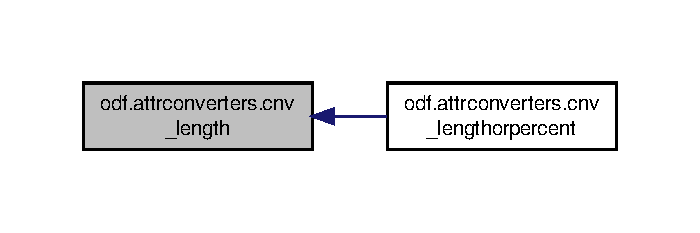
\includegraphics[width=336pt]{namespaceodf_1_1attrconverters_a4fde729e3a01d33ab946fb3ca8e1b1f1_icgraph}
\end{center}
\end{figure}


\hypertarget{namespaceodf_1_1attrconverters_adacce981267c9e1805396813a193b5db}{\index{odf\+::attrconverters@{odf\+::attrconverters}!cnv\+\_\+lengthorpercent@{cnv\+\_\+lengthorpercent}}
\index{cnv\+\_\+lengthorpercent@{cnv\+\_\+lengthorpercent}!odf\+::attrconverters@{odf\+::attrconverters}}
\subsubsection[{cnv\+\_\+lengthorpercent}]{\setlength{\rightskip}{0pt plus 5cm}def odf.\+attrconverters.\+cnv\+\_\+lengthorpercent (
\begin{DoxyParamCaption}
\item[{}]{attribute, }
\item[{}]{arg, }
\item[{}]{element}
\end{DoxyParamCaption}
)}}\label{namespaceodf_1_1attrconverters_adacce981267c9e1805396813a193b5db}


Definition at line 162 of file attrconverters.\+py.



Here is the call graph for this function\+:
\nopagebreak
\begin{figure}[H]
\begin{center}
\leavevmode
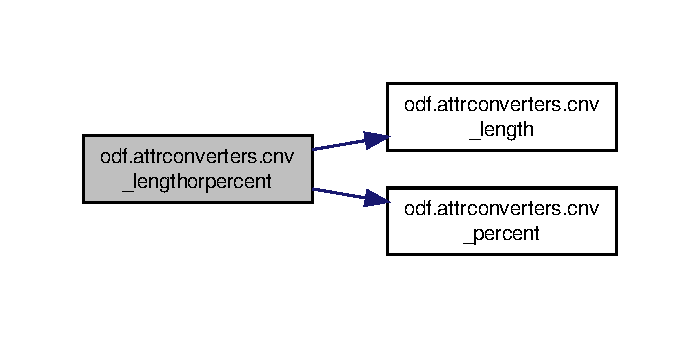
\includegraphics[width=336pt]{namespaceodf_1_1attrconverters_adacce981267c9e1805396813a193b5db_cgraph}
\end{center}
\end{figure}


\hypertarget{namespaceodf_1_1attrconverters_a14106eb750692910238b08052b753f99}{\index{odf\+::attrconverters@{odf\+::attrconverters}!cnv\+\_\+list\+\_\+linkage\+\_\+type@{cnv\+\_\+list\+\_\+linkage\+\_\+type}}
\index{cnv\+\_\+list\+\_\+linkage\+\_\+type@{cnv\+\_\+list\+\_\+linkage\+\_\+type}!odf\+::attrconverters@{odf\+::attrconverters}}
\subsubsection[{cnv\+\_\+list\+\_\+linkage\+\_\+type}]{\setlength{\rightskip}{0pt plus 5cm}def odf.\+attrconverters.\+cnv\+\_\+list\+\_\+linkage\+\_\+type (
\begin{DoxyParamCaption}
\item[{}]{attribute, }
\item[{}]{arg, }
\item[{}]{element}
\end{DoxyParamCaption}
)}}\label{namespaceodf_1_1attrconverters_a14106eb750692910238b08052b753f99}


Definition at line 172 of file attrconverters.\+py.

\hypertarget{namespaceodf_1_1attrconverters_a1e3f571e483f75017987c0dfb501acf0}{\index{odf\+::attrconverters@{odf\+::attrconverters}!cnv\+\_\+major\+\_\+minor@{cnv\+\_\+major\+\_\+minor}}
\index{cnv\+\_\+major\+\_\+minor@{cnv\+\_\+major\+\_\+minor}!odf\+::attrconverters@{odf\+::attrconverters}}
\subsubsection[{cnv\+\_\+major\+\_\+minor}]{\setlength{\rightskip}{0pt plus 5cm}def odf.\+attrconverters.\+cnv\+\_\+major\+\_\+minor (
\begin{DoxyParamCaption}
\item[{}]{attribute, }
\item[{}]{arg, }
\item[{}]{element}
\end{DoxyParamCaption}
)}}\label{namespaceodf_1_1attrconverters_a1e3f571e483f75017987c0dfb501acf0}


Definition at line 182 of file attrconverters.\+py.

\hypertarget{namespaceodf_1_1attrconverters_a4a9a41ce0c33aa08db57e3f68077cfba}{\index{odf\+::attrconverters@{odf\+::attrconverters}!cnv\+\_\+metavaluetype@{cnv\+\_\+metavaluetype}}
\index{cnv\+\_\+metavaluetype@{cnv\+\_\+metavaluetype}!odf\+::attrconverters@{odf\+::attrconverters}}
\subsubsection[{cnv\+\_\+metavaluetype}]{\setlength{\rightskip}{0pt plus 5cm}def odf.\+attrconverters.\+cnv\+\_\+metavaluetype (
\begin{DoxyParamCaption}
\item[{}]{attribute, }
\item[{}]{arg, }
\item[{}]{element}
\end{DoxyParamCaption}
)}}\label{namespaceodf_1_1attrconverters_a4a9a41ce0c33aa08db57e3f68077cfba}


Definition at line 177 of file attrconverters.\+py.

\hypertarget{namespaceodf_1_1attrconverters_a5e054049f615c37c24134589160af0e3}{\index{odf\+::attrconverters@{odf\+::attrconverters}!cnv\+\_\+namespaced\+Token@{cnv\+\_\+namespaced\+Token}}
\index{cnv\+\_\+namespaced\+Token@{cnv\+\_\+namespaced\+Token}!odf\+::attrconverters@{odf\+::attrconverters}}
\subsubsection[{cnv\+\_\+namespaced\+Token}]{\setlength{\rightskip}{0pt plus 5cm}def odf.\+attrconverters.\+cnv\+\_\+namespaced\+Token (
\begin{DoxyParamCaption}
\item[{}]{attribute, }
\item[{}]{arg, }
\item[{}]{element}
\end{DoxyParamCaption}
)}}\label{namespaceodf_1_1attrconverters_a5e054049f615c37c24134589160af0e3}


Definition at line 189 of file attrconverters.\+py.

\hypertarget{namespaceodf_1_1attrconverters_a62253f3e9de2349089df28cc66b27a07}{\index{odf\+::attrconverters@{odf\+::attrconverters}!cnv\+\_\+\+N\+C\+Name@{cnv\+\_\+\+N\+C\+Name}}
\index{cnv\+\_\+\+N\+C\+Name@{cnv\+\_\+\+N\+C\+Name}!odf\+::attrconverters@{odf\+::attrconverters}}
\subsubsection[{cnv\+\_\+\+N\+C\+Name}]{\setlength{\rightskip}{0pt plus 5cm}def odf.\+attrconverters.\+cnv\+\_\+\+N\+C\+Name (
\begin{DoxyParamCaption}
\item[{}]{attribute, }
\item[{}]{arg, }
\item[{}]{element}
\end{DoxyParamCaption}
)}}\label{namespaceodf_1_1attrconverters_a62253f3e9de2349089df28cc66b27a07}


N\+C\+Name is defined in \href{http://www.w3.org/TR/REC-xml-names/#NT-NCName}{\tt http\+://www.\+w3.\+org/\+T\+R/\+R\+E\+C-\/xml-\/names/\#\+N\+T-\/\+N\+C\+Name} Essentially an X\+M\+L name minus '\+:'. 



Definition at line 200 of file attrconverters.\+py.



Here is the call graph for this function\+:
\nopagebreak
\begin{figure}[H]
\begin{center}
\leavevmode
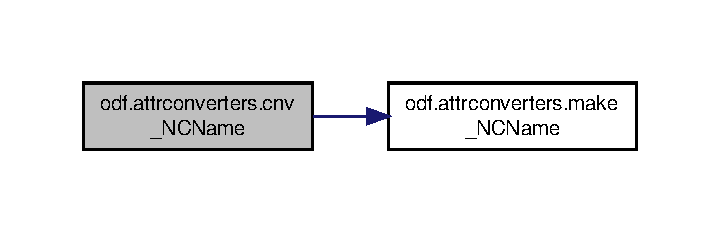
\includegraphics[width=346pt]{namespaceodf_1_1attrconverters_a62253f3e9de2349089df28cc66b27a07_cgraph}
\end{center}
\end{figure}


\hypertarget{namespaceodf_1_1attrconverters_a8559714891f5698310fe98661760c560}{\index{odf\+::attrconverters@{odf\+::attrconverters}!cnv\+\_\+\+N\+C\+Names@{cnv\+\_\+\+N\+C\+Names}}
\index{cnv\+\_\+\+N\+C\+Names@{cnv\+\_\+\+N\+C\+Names}!odf\+::attrconverters@{odf\+::attrconverters}}
\subsubsection[{cnv\+\_\+\+N\+C\+Names}]{\setlength{\rightskip}{0pt plus 5cm}def odf.\+attrconverters.\+cnv\+\_\+\+N\+C\+Names (
\begin{DoxyParamCaption}
\item[{}]{attribute, }
\item[{}]{arg, }
\item[{}]{element}
\end{DoxyParamCaption}
)}}\label{namespaceodf_1_1attrconverters_a8559714891f5698310fe98661760c560}


Definition at line 227 of file attrconverters.\+py.

\hypertarget{namespaceodf_1_1attrconverters_a6de0ebe883bd91d8328150e29b6d1883}{\index{odf\+::attrconverters@{odf\+::attrconverters}!cnv\+\_\+non\+Negative\+Integer@{cnv\+\_\+non\+Negative\+Integer}}
\index{cnv\+\_\+non\+Negative\+Integer@{cnv\+\_\+non\+Negative\+Integer}!odf\+::attrconverters@{odf\+::attrconverters}}
\subsubsection[{cnv\+\_\+non\+Negative\+Integer}]{\setlength{\rightskip}{0pt plus 5cm}def odf.\+attrconverters.\+cnv\+\_\+non\+Negative\+Integer (
\begin{DoxyParamCaption}
\item[{}]{attribute, }
\item[{}]{arg, }
\item[{}]{element}
\end{DoxyParamCaption}
)}}\label{namespaceodf_1_1attrconverters_a6de0ebe883bd91d8328150e29b6d1883}


Definition at line 230 of file attrconverters.\+py.

\hypertarget{namespaceodf_1_1attrconverters_aac11979c1416aabac74a65e5ba0725a0}{\index{odf\+::attrconverters@{odf\+::attrconverters}!cnv\+\_\+percent@{cnv\+\_\+percent}}
\index{cnv\+\_\+percent@{cnv\+\_\+percent}!odf\+::attrconverters@{odf\+::attrconverters}}
\subsubsection[{cnv\+\_\+percent}]{\setlength{\rightskip}{0pt plus 5cm}def odf.\+attrconverters.\+cnv\+\_\+percent (
\begin{DoxyParamCaption}
\item[{}]{attribute, }
\item[{}]{arg, }
\item[{}]{element}
\end{DoxyParamCaption}
)}}\label{namespaceodf_1_1attrconverters_aac11979c1416aabac74a65e5ba0725a0}


Definition at line 235 of file attrconverters.\+py.



Here is the caller graph for this function\+:
\nopagebreak
\begin{figure}[H]
\begin{center}
\leavevmode
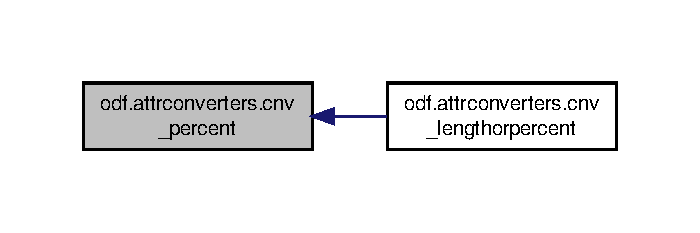
\includegraphics[width=336pt]{namespaceodf_1_1attrconverters_aac11979c1416aabac74a65e5ba0725a0_icgraph}
\end{center}
\end{figure}


\hypertarget{namespaceodf_1_1attrconverters_a27d9ea13a2e1a5add722743f1fa756f5}{\index{odf\+::attrconverters@{odf\+::attrconverters}!cnv\+\_\+points@{cnv\+\_\+points}}
\index{cnv\+\_\+points@{cnv\+\_\+points}!odf\+::attrconverters@{odf\+::attrconverters}}
\subsubsection[{cnv\+\_\+points}]{\setlength{\rightskip}{0pt plus 5cm}def odf.\+attrconverters.\+cnv\+\_\+points (
\begin{DoxyParamCaption}
\item[{}]{attribute, }
\item[{}]{arg, }
\item[{}]{element}
\end{DoxyParamCaption}
)}}\label{namespaceodf_1_1attrconverters_a27d9ea13a2e1a5add722743f1fa756f5}


Definition at line 244 of file attrconverters.\+py.

\hypertarget{namespaceodf_1_1attrconverters_a29b8e7d897025f975c135179d5cf7321}{\index{odf\+::attrconverters@{odf\+::attrconverters}!cnv\+\_\+positive\+Integer@{cnv\+\_\+positive\+Integer}}
\index{cnv\+\_\+positive\+Integer@{cnv\+\_\+positive\+Integer}!odf\+::attrconverters@{odf\+::attrconverters}}
\subsubsection[{cnv\+\_\+positive\+Integer}]{\setlength{\rightskip}{0pt plus 5cm}def odf.\+attrconverters.\+cnv\+\_\+positive\+Integer (
\begin{DoxyParamCaption}
\item[{}]{attribute, }
\item[{}]{arg, }
\item[{}]{element}
\end{DoxyParamCaption}
)}}\label{namespaceodf_1_1attrconverters_a29b8e7d897025f975c135179d5cf7321}


Definition at line 257 of file attrconverters.\+py.

\hypertarget{namespaceodf_1_1attrconverters_aea7dfa16c558fceaa163879ee587cce8}{\index{odf\+::attrconverters@{odf\+::attrconverters}!cnv\+\_\+row\+Or\+Col@{cnv\+\_\+row\+Or\+Col}}
\index{cnv\+\_\+row\+Or\+Col@{cnv\+\_\+row\+Or\+Col}!odf\+::attrconverters@{odf\+::attrconverters}}
\subsubsection[{cnv\+\_\+row\+Or\+Col}]{\setlength{\rightskip}{0pt plus 5cm}def odf.\+attrconverters.\+cnv\+\_\+row\+Or\+Col (
\begin{DoxyParamCaption}
\item[{}]{attribute, }
\item[{}]{arg, }
\item[{}]{element}
\end{DoxyParamCaption}
)}}\label{namespaceodf_1_1attrconverters_aea7dfa16c558fceaa163879ee587cce8}


Definition at line 260 of file attrconverters.\+py.

\hypertarget{namespaceodf_1_1attrconverters_a072f568e8950c53f5a4a6912a5ca175c}{\index{odf\+::attrconverters@{odf\+::attrconverters}!cnv\+\_\+string@{cnv\+\_\+string}}
\index{cnv\+\_\+string@{cnv\+\_\+string}!odf\+::attrconverters@{odf\+::attrconverters}}
\subsubsection[{cnv\+\_\+string}]{\setlength{\rightskip}{0pt plus 5cm}def odf.\+attrconverters.\+cnv\+\_\+string (
\begin{DoxyParamCaption}
\item[{}]{attribute, }
\item[{}]{arg, }
\item[{}]{element}
\end{DoxyParamCaption}
)}}\label{namespaceodf_1_1attrconverters_a072f568e8950c53f5a4a6912a5ca175c}


Definition at line 265 of file attrconverters.\+py.

\hypertarget{namespaceodf_1_1attrconverters_a9e734cce61f54f6cf18a9e14b485cbd1}{\index{odf\+::attrconverters@{odf\+::attrconverters}!cnv\+\_\+stroke\+\_\+linecap@{cnv\+\_\+stroke\+\_\+linecap}}
\index{cnv\+\_\+stroke\+\_\+linecap@{cnv\+\_\+stroke\+\_\+linecap}!odf\+::attrconverters@{odf\+::attrconverters}}
\subsubsection[{cnv\+\_\+stroke\+\_\+linecap}]{\setlength{\rightskip}{0pt plus 5cm}def odf.\+attrconverters.\+cnv\+\_\+stroke\+\_\+linecap (
\begin{DoxyParamCaption}
\item[{}]{attribute, }
\item[{}]{arg, }
\item[{}]{element}
\end{DoxyParamCaption}
)}}\label{namespaceodf_1_1attrconverters_a9e734cce61f54f6cf18a9e14b485cbd1}


Definition at line 271 of file attrconverters.\+py.

\hypertarget{namespaceodf_1_1attrconverters_a20017beeb1514762702703c37e09c2da}{\index{odf\+::attrconverters@{odf\+::attrconverters}!cnv\+\_\+\+Style\+Name\+Ref@{cnv\+\_\+\+Style\+Name\+Ref}}
\index{cnv\+\_\+\+Style\+Name\+Ref@{cnv\+\_\+\+Style\+Name\+Ref}!odf\+::attrconverters@{odf\+::attrconverters}}
\subsubsection[{cnv\+\_\+\+Style\+Name\+Ref}]{\setlength{\rightskip}{0pt plus 5cm}def odf.\+attrconverters.\+cnv\+\_\+\+Style\+Name\+Ref (
\begin{DoxyParamCaption}
\item[{}]{attribute, }
\item[{}]{arg, }
\item[{}]{element}
\end{DoxyParamCaption}
)}}\label{namespaceodf_1_1attrconverters_a20017beeb1514762702703c37e09c2da}


Definition at line 210 of file attrconverters.\+py.

\hypertarget{namespaceodf_1_1attrconverters_a332c61e3ebc751ae0d2204fe011d687b}{\index{odf\+::attrconverters@{odf\+::attrconverters}!cnv\+\_\+textnoteclass@{cnv\+\_\+textnoteclass}}
\index{cnv\+\_\+textnoteclass@{cnv\+\_\+textnoteclass}!odf\+::attrconverters@{odf\+::attrconverters}}
\subsubsection[{cnv\+\_\+textnoteclass}]{\setlength{\rightskip}{0pt plus 5cm}def odf.\+attrconverters.\+cnv\+\_\+textnoteclass (
\begin{DoxyParamCaption}
\item[{}]{attribute, }
\item[{}]{arg, }
\item[{}]{element}
\end{DoxyParamCaption}
)}}\label{namespaceodf_1_1attrconverters_a332c61e3ebc751ae0d2204fe011d687b}


Definition at line 276 of file attrconverters.\+py.

\hypertarget{namespaceodf_1_1attrconverters_ab7ae6299ddbe0d3f140c1d614e14d3d3}{\index{odf\+::attrconverters@{odf\+::attrconverters}!cnv\+\_\+time@{cnv\+\_\+time}}
\index{cnv\+\_\+time@{cnv\+\_\+time}!odf\+::attrconverters@{odf\+::attrconverters}}
\subsubsection[{cnv\+\_\+time}]{\setlength{\rightskip}{0pt plus 5cm}def odf.\+attrconverters.\+cnv\+\_\+time (
\begin{DoxyParamCaption}
\item[{}]{attribute, }
\item[{}]{arg, }
\item[{}]{element}
\end{DoxyParamCaption}
)}}\label{namespaceodf_1_1attrconverters_ab7ae6299ddbe0d3f140c1d614e14d3d3}


Definition at line 282 of file attrconverters.\+py.

\hypertarget{namespaceodf_1_1attrconverters_aba85383db54b917bfa67ff161d606c92}{\index{odf\+::attrconverters@{odf\+::attrconverters}!cnv\+\_\+token@{cnv\+\_\+token}}
\index{cnv\+\_\+token@{cnv\+\_\+token}!odf\+::attrconverters@{odf\+::attrconverters}}
\subsubsection[{cnv\+\_\+token}]{\setlength{\rightskip}{0pt plus 5cm}def odf.\+attrconverters.\+cnv\+\_\+token (
\begin{DoxyParamCaption}
\item[{}]{attribute, }
\item[{}]{arg, }
\item[{}]{element}
\end{DoxyParamCaption}
)}}\label{namespaceodf_1_1attrconverters_aba85383db54b917bfa67ff161d606c92}


Definition at line 285 of file attrconverters.\+py.

\hypertarget{namespaceodf_1_1attrconverters_ad3126045f15c7f1eb1d1fa42428bd9bf}{\index{odf\+::attrconverters@{odf\+::attrconverters}!cnv\+\_\+viewbox@{cnv\+\_\+viewbox}}
\index{cnv\+\_\+viewbox@{cnv\+\_\+viewbox}!odf\+::attrconverters@{odf\+::attrconverters}}
\subsubsection[{cnv\+\_\+viewbox}]{\setlength{\rightskip}{0pt plus 5cm}def odf.\+attrconverters.\+cnv\+\_\+viewbox (
\begin{DoxyParamCaption}
\item[{}]{attribute, }
\item[{}]{arg, }
\item[{}]{element}
\end{DoxyParamCaption}
)}}\label{namespaceodf_1_1attrconverters_ad3126045f15c7f1eb1d1fa42428bd9bf}


Definition at line 290 of file attrconverters.\+py.

\hypertarget{namespaceodf_1_1attrconverters_a2102b975dd86f365f5776756fa73c992}{\index{odf\+::attrconverters@{odf\+::attrconverters}!cnv\+\_\+xlinkshow@{cnv\+\_\+xlinkshow}}
\index{cnv\+\_\+xlinkshow@{cnv\+\_\+xlinkshow}!odf\+::attrconverters@{odf\+::attrconverters}}
\subsubsection[{cnv\+\_\+xlinkshow}]{\setlength{\rightskip}{0pt plus 5cm}def odf.\+attrconverters.\+cnv\+\_\+xlinkshow (
\begin{DoxyParamCaption}
\item[{}]{attribute, }
\item[{}]{arg, }
\item[{}]{element}
\end{DoxyParamCaption}
)}}\label{namespaceodf_1_1attrconverters_a2102b975dd86f365f5776756fa73c992}


Definition at line 296 of file attrconverters.\+py.

\hypertarget{namespaceodf_1_1attrconverters_a2cb861fbdd6bd0094fe5042b4355d918}{\index{odf\+::attrconverters@{odf\+::attrconverters}!cnv\+\_\+xlinktype@{cnv\+\_\+xlinktype}}
\index{cnv\+\_\+xlinktype@{cnv\+\_\+xlinktype}!odf\+::attrconverters@{odf\+::attrconverters}}
\subsubsection[{cnv\+\_\+xlinktype}]{\setlength{\rightskip}{0pt plus 5cm}def odf.\+attrconverters.\+cnv\+\_\+xlinktype (
\begin{DoxyParamCaption}
\item[{}]{attribute, }
\item[{}]{arg, }
\item[{}]{element}
\end{DoxyParamCaption}
)}}\label{namespaceodf_1_1attrconverters_a2cb861fbdd6bd0094fe5042b4355d918}


Definition at line 301 of file attrconverters.\+py.

\hypertarget{namespaceodf_1_1attrconverters_a6755b6a5aedaf9689050ad84c4ede320}{\index{odf\+::attrconverters@{odf\+::attrconverters}!make\+\_\+\+N\+C\+Name@{make\+\_\+\+N\+C\+Name}}
\index{make\+\_\+\+N\+C\+Name@{make\+\_\+\+N\+C\+Name}!odf\+::attrconverters@{odf\+::attrconverters}}
\subsubsection[{make\+\_\+\+N\+C\+Name}]{\setlength{\rightskip}{0pt plus 5cm}def odf.\+attrconverters.\+make\+\_\+\+N\+C\+Name (
\begin{DoxyParamCaption}
\item[{}]{arg}
\end{DoxyParamCaption}
)}}\label{namespaceodf_1_1attrconverters_a6755b6a5aedaf9689050ad84c4ede320}


Definition at line 29 of file attrconverters.\+py.



Here is the caller graph for this function\+:
\nopagebreak
\begin{figure}[H]
\begin{center}
\leavevmode
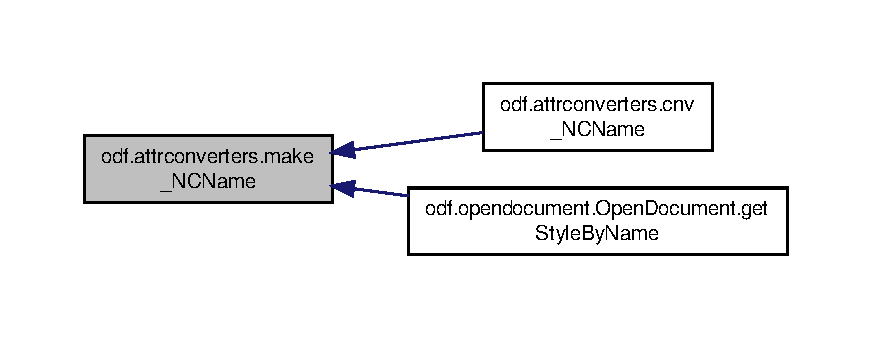
\includegraphics[width=350pt]{namespaceodf_1_1attrconverters_a6755b6a5aedaf9689050ad84c4ede320_icgraph}
\end{center}
\end{figure}




\subsection{Variable Documentation}
\hypertarget{namespaceodf_1_1attrconverters_aa546908cd138bdd3bd7fd61e75ebc87f}{\index{odf\+::attrconverters@{odf\+::attrconverters}!attrconverters@{attrconverters}}
\index{attrconverters@{attrconverters}!odf\+::attrconverters@{odf\+::attrconverters}}
\subsubsection[{attrconverters}]{\setlength{\rightskip}{0pt plus 5cm}dictionary odf.\+attrconverters.\+attrconverters}}\label{namespaceodf_1_1attrconverters_aa546908cd138bdd3bd7fd61e75ebc87f}


Definition at line 307 of file attrconverters.\+py.

\hypertarget{namespaceodf_1_1attrconverters_a942ee7e8270b6cb9f232b85d91f167cc}{\index{odf\+::attrconverters@{odf\+::attrconverters}!pattern\+\_\+color@{pattern\+\_\+color}}
\index{pattern\+\_\+color@{pattern\+\_\+color}!odf\+::attrconverters@{odf\+::attrconverters}}
\subsubsection[{pattern\+\_\+color}]{\setlength{\rightskip}{0pt plus 5cm}tuple odf.\+attrconverters.\+pattern\+\_\+color = re.\+compile(r'\#\mbox{[}0-\/9a-\/f\+A-\/\+F\mbox{]}\{6\}')}}\label{namespaceodf_1_1attrconverters_a942ee7e8270b6cb9f232b85d91f167cc}


Definition at line 26 of file attrconverters.\+py.

\hypertarget{namespaceodf_1_1attrconverters_ad9906afdc77dcf5ec8024ddea8af2cd3}{\index{odf\+::attrconverters@{odf\+::attrconverters}!pattern\+\_\+language@{pattern\+\_\+language}}
\index{pattern\+\_\+language@{pattern\+\_\+language}!odf\+::attrconverters@{odf\+::attrconverters}}
\subsubsection[{pattern\+\_\+language}]{\setlength{\rightskip}{0pt plus 5cm}tuple odf.\+attrconverters.\+pattern\+\_\+language = re.\+compile(r'\mbox{[}a-\/z\+A-\/Z\mbox{]}\{1,8\}(-\/\mbox{[}a-\/z\+A-\/Z0-\/9\mbox{]}\{1,8\})$\ast$')}}\label{namespaceodf_1_1attrconverters_ad9906afdc77dcf5ec8024ddea8af2cd3}


Definition at line 137 of file attrconverters.\+py.

\hypertarget{namespaceodf_1_1attrconverters_aa90a2e19771f728a7a760efaeb548853}{\index{odf\+::attrconverters@{odf\+::attrconverters}!pattern\+\_\+length@{pattern\+\_\+length}}
\index{pattern\+\_\+length@{pattern\+\_\+length}!odf\+::attrconverters@{odf\+::attrconverters}}
\subsubsection[{pattern\+\_\+length}]{\setlength{\rightskip}{0pt plus 5cm}tuple odf.\+attrconverters.\+pattern\+\_\+length = re.\+compile(r'-\/?(\mbox{[}0-\/9\mbox{]}+(\textbackslash{}.\mbox{[}0-\/9\mbox{]}$\ast$)?$\vert$\textbackslash{}.\mbox{[}0-\/9\mbox{]}+)((cm)$\vert$(mm)$\vert$(in)$\vert$(pt)$\vert$(pc)$\vert$(px))')}}\label{namespaceodf_1_1attrconverters_aa90a2e19771f728a7a760efaeb548853}


Definition at line 150 of file attrconverters.\+py.

\hypertarget{namespaceodf_1_1attrconverters_a8b1acec5f51ab504076429de4a44e126}{\index{odf\+::attrconverters@{odf\+::attrconverters}!pattern\+\_\+namespaced\+Token@{pattern\+\_\+namespaced\+Token}}
\index{pattern\+\_\+namespaced\+Token@{pattern\+\_\+namespaced\+Token}!odf\+::attrconverters@{odf\+::attrconverters}}
\subsubsection[{pattern\+\_\+namespaced\+Token}]{\setlength{\rightskip}{0pt plus 5cm}tuple odf.\+attrconverters.\+pattern\+\_\+namespaced\+Token = re.\+compile(r'\mbox{[}0-\/9a-\/z\+A-\/\+Z\+\_\+\mbox{]}+\+:\mbox{[}0-\/9a-\/z\+A-\/\+Z.\+\_\+\textbackslash{}-\/\mbox{]}+')}}\label{namespaceodf_1_1attrconverters_a8b1acec5f51ab504076429de4a44e126}


Definition at line 187 of file attrconverters.\+py.

\hypertarget{namespaceodf_1_1attrconverters_a579361611ccfad779029c701add3beac}{\index{odf\+::attrconverters@{odf\+::attrconverters}!pattern\+\_\+percent@{pattern\+\_\+percent}}
\index{pattern\+\_\+percent@{pattern\+\_\+percent}!odf\+::attrconverters@{odf\+::attrconverters}}
\subsubsection[{pattern\+\_\+percent}]{\setlength{\rightskip}{0pt plus 5cm}tuple odf.\+attrconverters.\+pattern\+\_\+percent = re.\+compile(r'-\/?(\mbox{[}0-\/9\mbox{]}+(\textbackslash{}.\mbox{[}0-\/9\mbox{]}$\ast$)?$\vert$\textbackslash{}.\mbox{[}0-\/9\mbox{]}+)\%')}}\label{namespaceodf_1_1attrconverters_a579361611ccfad779029c701add3beac}


Definition at line 233 of file attrconverters.\+py.

\hypertarget{namespaceodf_1_1attrconverters_aba1cc76213c8ca3e229a93e09ac6f4ee}{\index{odf\+::attrconverters@{odf\+::attrconverters}!pattern\+\_\+points@{pattern\+\_\+points}}
\index{pattern\+\_\+points@{pattern\+\_\+points}!odf\+::attrconverters@{odf\+::attrconverters}}
\subsubsection[{pattern\+\_\+points}]{\setlength{\rightskip}{0pt plus 5cm}tuple odf.\+attrconverters.\+pattern\+\_\+points = re.\+compile(r'-\/?\mbox{[}0-\/9\mbox{]}+,-\/?\mbox{[}0-\/9\mbox{]}+(\mbox{[} \mbox{]}+-\/?\mbox{[}0-\/9\mbox{]}+,-\/?\mbox{[}0-\/9\mbox{]}+)$\ast$')}}\label{namespaceodf_1_1attrconverters_aba1cc76213c8ca3e229a93e09ac6f4ee}


Definition at line 242 of file attrconverters.\+py.

\hypertarget{namespaceodf_1_1attrconverters_adcdf5feb55fad2176b65fc447fae6957}{\index{odf\+::attrconverters@{odf\+::attrconverters}!pattern\+\_\+vector3\+D@{pattern\+\_\+vector3\+D}}
\index{pattern\+\_\+vector3\+D@{pattern\+\_\+vector3\+D}!odf\+::attrconverters@{odf\+::attrconverters}}
\subsubsection[{pattern\+\_\+vector3\+D}]{\setlength{\rightskip}{0pt plus 5cm}tuple odf.\+attrconverters.\+pattern\+\_\+vector3\+D = re.\+compile(r'\textbackslash{}(\mbox{[} \mbox{]}$\ast$-\/?(\mbox{[}0-\/9\mbox{]}+(\textbackslash{}.\mbox{[}0-\/9\mbox{]}$\ast$)?$\vert$\textbackslash{}.\mbox{[}0-\/9\mbox{]}+)(\mbox{[} \mbox{]}+-\/?(\mbox{[}0-\/9\mbox{]}+(\textbackslash{}.\mbox{[}0-\/9\mbox{]}$\ast$)?$\vert$\textbackslash{}.\mbox{[}0-\/9\mbox{]}+))\{2\}\mbox{[} \mbox{]}$\ast$\textbackslash{})')}}\label{namespaceodf_1_1attrconverters_adcdf5feb55fad2176b65fc447fae6957}


Definition at line 27 of file attrconverters.\+py.

\hypertarget{namespaceodf_1_1attrconverters_a3df24b76956ae1cb73bf3fd649d558a3}{\index{odf\+::attrconverters@{odf\+::attrconverters}!pattern\+\_\+viewbox@{pattern\+\_\+viewbox}}
\index{pattern\+\_\+viewbox@{pattern\+\_\+viewbox}!odf\+::attrconverters@{odf\+::attrconverters}}
\subsubsection[{pattern\+\_\+viewbox}]{\setlength{\rightskip}{0pt plus 5cm}tuple odf.\+attrconverters.\+pattern\+\_\+viewbox = re.\+compile(r'-\/?\mbox{[}0-\/9\mbox{]}+(\mbox{[} \mbox{]}+-\/?\mbox{[}0-\/9\mbox{]}+)\{3\}\$')}}\label{namespaceodf_1_1attrconverters_a3df24b76956ae1cb73bf3fd649d558a3}


Definition at line 288 of file attrconverters.\+py.


\hypertarget{namespaceodf_1_1chart}{\section{odf.\+chart Namespace Reference}
\label{namespaceodf_1_1chart}\index{odf.\+chart@{odf.\+chart}}
}
\subsection*{Functions}
\begin{DoxyCompactItemize}
\item 
def \hyperlink{namespaceodf_1_1chart_a329874378a6b8d3670eb489cfc44f651}{Axis}
\item 
def \hyperlink{namespaceodf_1_1chart_aa82f78545efd652517ccc8717e7d40dd}{Categories}
\item 
def \hyperlink{namespaceodf_1_1chart_a68803758f9df5a37ff0dfadf736d38e0}{Chart}
\item 
def \hyperlink{namespaceodf_1_1chart_a179d1eaa90b948cceb2bbf4db776c6db}{Data\+Label}
\item 
def \hyperlink{namespaceodf_1_1chart_a1934c7d5dfbbe6a0e1d035f9559609d9}{Data\+Point}
\item 
def \hyperlink{namespaceodf_1_1chart_a069febad17f28421479d162744425132}{Domain}
\item 
def \hyperlink{namespaceodf_1_1chart_a521b13c9b125eab65fce28f5cd204248}{Equation}
\item 
def \hyperlink{namespaceodf_1_1chart_af8fb9968af1a26db725c3a7a25b659cf}{Error\+Indicator}
\item 
def \hyperlink{namespaceodf_1_1chart_aac2c903446e655fef725fbe15b501c24}{Floor}
\item 
def \hyperlink{namespaceodf_1_1chart_ae9f21dda3937bd3326ea5f9628fa9910}{Footer}
\item 
def \hyperlink{namespaceodf_1_1chart_a869f1e52109d7d02fdb2e6afa0486bc4}{Grid}
\item 
def \hyperlink{namespaceodf_1_1chart_a9a01025fc3d47bd002655343f1019eae}{Label\+Separator}
\item 
def \hyperlink{namespaceodf_1_1chart_a87d2416f717c7bcde696048089eb7c7b}{Legend}
\item 
def \hyperlink{namespaceodf_1_1chart_a21900789caa86f6a8e7ca11c47d697de}{Mean\+Value}
\item 
def \hyperlink{namespaceodf_1_1chart_af23c82b5fc6692cd81c51282643cd5b1}{Plot\+Area}
\item 
def \hyperlink{namespaceodf_1_1chart_a4317ee1ece08c161d7eb0b0374a5bcaf}{Regression\+Curve}
\item 
def \hyperlink{namespaceodf_1_1chart_adb09a17748f971fc823bdc10c518c611}{Series}
\item 
def \hyperlink{namespaceodf_1_1chart_ae76e7238b43dcc8744745065054e4f23}{Stock\+Gain\+Marker}
\item 
def \hyperlink{namespaceodf_1_1chart_afb120252c94ddcfe4e6e266282d9c64c}{Stock\+Loss\+Marker}
\item 
def \hyperlink{namespaceodf_1_1chart_a67610a5849288c96576c82b17f91c8c9}{Stock\+Range\+Line}
\item 
def \hyperlink{namespaceodf_1_1chart_ae91903f8543ffa247125ebb19d8b2fa0}{Subtitle}
\item 
def \hyperlink{namespaceodf_1_1chart_ae6a4eb755b9a4df720ac8972a2147c85}{Symbol\+Image}
\item 
def \hyperlink{namespaceodf_1_1chart_ad684313f079591a29155ca303310f5d6}{Title}
\item 
def \hyperlink{namespaceodf_1_1chart_ad7d996753e59626d2e500f5cdf98d7ec}{Wall}
\end{DoxyCompactItemize}


\subsection{Function Documentation}
\hypertarget{namespaceodf_1_1chart_a329874378a6b8d3670eb489cfc44f651}{\index{odf\+::chart@{odf\+::chart}!Axis@{Axis}}
\index{Axis@{Axis}!odf\+::chart@{odf\+::chart}}
\subsubsection[{Axis}]{\setlength{\rightskip}{0pt plus 5cm}def odf.\+chart.\+Axis (
\begin{DoxyParamCaption}
\item[{}]{args}
\end{DoxyParamCaption}
)}}\label{namespaceodf_1_1chart_a329874378a6b8d3670eb489cfc44f651}


Definition at line 25 of file chart.\+py.

\hypertarget{namespaceodf_1_1chart_aa82f78545efd652517ccc8717e7d40dd}{\index{odf\+::chart@{odf\+::chart}!Categories@{Categories}}
\index{Categories@{Categories}!odf\+::chart@{odf\+::chart}}
\subsubsection[{Categories}]{\setlength{\rightskip}{0pt plus 5cm}def odf.\+chart.\+Categories (
\begin{DoxyParamCaption}
\item[{}]{args}
\end{DoxyParamCaption}
)}}\label{namespaceodf_1_1chart_aa82f78545efd652517ccc8717e7d40dd}


Definition at line 28 of file chart.\+py.

\hypertarget{namespaceodf_1_1chart_a68803758f9df5a37ff0dfadf736d38e0}{\index{odf\+::chart@{odf\+::chart}!Chart@{Chart}}
\index{Chart@{Chart}!odf\+::chart@{odf\+::chart}}
\subsubsection[{Chart}]{\setlength{\rightskip}{0pt plus 5cm}def odf.\+chart.\+Chart (
\begin{DoxyParamCaption}
\item[{}]{args}
\end{DoxyParamCaption}
)}}\label{namespaceodf_1_1chart_a68803758f9df5a37ff0dfadf736d38e0}


Definition at line 31 of file chart.\+py.



Here is the caller graph for this function\+:
\nopagebreak
\begin{figure}[H]
\begin{center}
\leavevmode
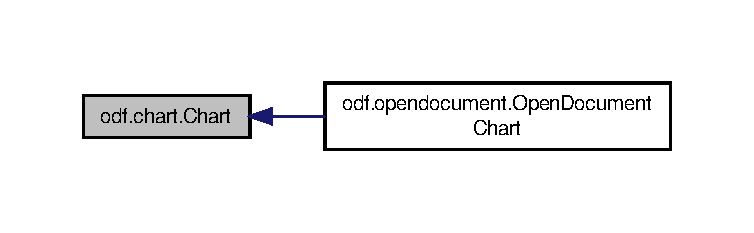
\includegraphics[width=350pt]{namespaceodf_1_1chart_a68803758f9df5a37ff0dfadf736d38e0_icgraph}
\end{center}
\end{figure}


\hypertarget{namespaceodf_1_1chart_a179d1eaa90b948cceb2bbf4db776c6db}{\index{odf\+::chart@{odf\+::chart}!Data\+Label@{Data\+Label}}
\index{Data\+Label@{Data\+Label}!odf\+::chart@{odf\+::chart}}
\subsubsection[{Data\+Label}]{\setlength{\rightskip}{0pt plus 5cm}def odf.\+chart.\+Data\+Label (
\begin{DoxyParamCaption}
\item[{}]{args}
\end{DoxyParamCaption}
)}}\label{namespaceodf_1_1chart_a179d1eaa90b948cceb2bbf4db776c6db}


Definition at line 34 of file chart.\+py.

\hypertarget{namespaceodf_1_1chart_a1934c7d5dfbbe6a0e1d035f9559609d9}{\index{odf\+::chart@{odf\+::chart}!Data\+Point@{Data\+Point}}
\index{Data\+Point@{Data\+Point}!odf\+::chart@{odf\+::chart}}
\subsubsection[{Data\+Point}]{\setlength{\rightskip}{0pt plus 5cm}def odf.\+chart.\+Data\+Point (
\begin{DoxyParamCaption}
\item[{}]{args}
\end{DoxyParamCaption}
)}}\label{namespaceodf_1_1chart_a1934c7d5dfbbe6a0e1d035f9559609d9}


Definition at line 37 of file chart.\+py.

\hypertarget{namespaceodf_1_1chart_a069febad17f28421479d162744425132}{\index{odf\+::chart@{odf\+::chart}!Domain@{Domain}}
\index{Domain@{Domain}!odf\+::chart@{odf\+::chart}}
\subsubsection[{Domain}]{\setlength{\rightskip}{0pt plus 5cm}def odf.\+chart.\+Domain (
\begin{DoxyParamCaption}
\item[{}]{args}
\end{DoxyParamCaption}
)}}\label{namespaceodf_1_1chart_a069febad17f28421479d162744425132}


Definition at line 40 of file chart.\+py.

\hypertarget{namespaceodf_1_1chart_a521b13c9b125eab65fce28f5cd204248}{\index{odf\+::chart@{odf\+::chart}!Equation@{Equation}}
\index{Equation@{Equation}!odf\+::chart@{odf\+::chart}}
\subsubsection[{Equation}]{\setlength{\rightskip}{0pt plus 5cm}def odf.\+chart.\+Equation (
\begin{DoxyParamCaption}
\item[{}]{args}
\end{DoxyParamCaption}
)}}\label{namespaceodf_1_1chart_a521b13c9b125eab65fce28f5cd204248}


Definition at line 43 of file chart.\+py.

\hypertarget{namespaceodf_1_1chart_af8fb9968af1a26db725c3a7a25b659cf}{\index{odf\+::chart@{odf\+::chart}!Error\+Indicator@{Error\+Indicator}}
\index{Error\+Indicator@{Error\+Indicator}!odf\+::chart@{odf\+::chart}}
\subsubsection[{Error\+Indicator}]{\setlength{\rightskip}{0pt plus 5cm}def odf.\+chart.\+Error\+Indicator (
\begin{DoxyParamCaption}
\item[{}]{args}
\end{DoxyParamCaption}
)}}\label{namespaceodf_1_1chart_af8fb9968af1a26db725c3a7a25b659cf}


Definition at line 46 of file chart.\+py.

\hypertarget{namespaceodf_1_1chart_aac2c903446e655fef725fbe15b501c24}{\index{odf\+::chart@{odf\+::chart}!Floor@{Floor}}
\index{Floor@{Floor}!odf\+::chart@{odf\+::chart}}
\subsubsection[{Floor}]{\setlength{\rightskip}{0pt plus 5cm}def odf.\+chart.\+Floor (
\begin{DoxyParamCaption}
\item[{}]{args}
\end{DoxyParamCaption}
)}}\label{namespaceodf_1_1chart_aac2c903446e655fef725fbe15b501c24}


Definition at line 49 of file chart.\+py.

\hypertarget{namespaceodf_1_1chart_ae9f21dda3937bd3326ea5f9628fa9910}{\index{odf\+::chart@{odf\+::chart}!Footer@{Footer}}
\index{Footer@{Footer}!odf\+::chart@{odf\+::chart}}
\subsubsection[{Footer}]{\setlength{\rightskip}{0pt plus 5cm}def odf.\+chart.\+Footer (
\begin{DoxyParamCaption}
\item[{}]{args}
\end{DoxyParamCaption}
)}}\label{namespaceodf_1_1chart_ae9f21dda3937bd3326ea5f9628fa9910}


Definition at line 52 of file chart.\+py.

\hypertarget{namespaceodf_1_1chart_a869f1e52109d7d02fdb2e6afa0486bc4}{\index{odf\+::chart@{odf\+::chart}!Grid@{Grid}}
\index{Grid@{Grid}!odf\+::chart@{odf\+::chart}}
\subsubsection[{Grid}]{\setlength{\rightskip}{0pt plus 5cm}def odf.\+chart.\+Grid (
\begin{DoxyParamCaption}
\item[{}]{args}
\end{DoxyParamCaption}
)}}\label{namespaceodf_1_1chart_a869f1e52109d7d02fdb2e6afa0486bc4}


Definition at line 55 of file chart.\+py.

\hypertarget{namespaceodf_1_1chart_a9a01025fc3d47bd002655343f1019eae}{\index{odf\+::chart@{odf\+::chart}!Label\+Separator@{Label\+Separator}}
\index{Label\+Separator@{Label\+Separator}!odf\+::chart@{odf\+::chart}}
\subsubsection[{Label\+Separator}]{\setlength{\rightskip}{0pt plus 5cm}def odf.\+chart.\+Label\+Separator (
\begin{DoxyParamCaption}
\item[{}]{args}
\end{DoxyParamCaption}
)}}\label{namespaceodf_1_1chart_a9a01025fc3d47bd002655343f1019eae}


Definition at line 58 of file chart.\+py.

\hypertarget{namespaceodf_1_1chart_a87d2416f717c7bcde696048089eb7c7b}{\index{odf\+::chart@{odf\+::chart}!Legend@{Legend}}
\index{Legend@{Legend}!odf\+::chart@{odf\+::chart}}
\subsubsection[{Legend}]{\setlength{\rightskip}{0pt plus 5cm}def odf.\+chart.\+Legend (
\begin{DoxyParamCaption}
\item[{}]{args}
\end{DoxyParamCaption}
)}}\label{namespaceodf_1_1chart_a87d2416f717c7bcde696048089eb7c7b}


Definition at line 61 of file chart.\+py.

\hypertarget{namespaceodf_1_1chart_a21900789caa86f6a8e7ca11c47d697de}{\index{odf\+::chart@{odf\+::chart}!Mean\+Value@{Mean\+Value}}
\index{Mean\+Value@{Mean\+Value}!odf\+::chart@{odf\+::chart}}
\subsubsection[{Mean\+Value}]{\setlength{\rightskip}{0pt plus 5cm}def odf.\+chart.\+Mean\+Value (
\begin{DoxyParamCaption}
\item[{}]{args}
\end{DoxyParamCaption}
)}}\label{namespaceodf_1_1chart_a21900789caa86f6a8e7ca11c47d697de}


Definition at line 64 of file chart.\+py.

\hypertarget{namespaceodf_1_1chart_af23c82b5fc6692cd81c51282643cd5b1}{\index{odf\+::chart@{odf\+::chart}!Plot\+Area@{Plot\+Area}}
\index{Plot\+Area@{Plot\+Area}!odf\+::chart@{odf\+::chart}}
\subsubsection[{Plot\+Area}]{\setlength{\rightskip}{0pt plus 5cm}def odf.\+chart.\+Plot\+Area (
\begin{DoxyParamCaption}
\item[{}]{args}
\end{DoxyParamCaption}
)}}\label{namespaceodf_1_1chart_af23c82b5fc6692cd81c51282643cd5b1}


Definition at line 67 of file chart.\+py.

\hypertarget{namespaceodf_1_1chart_a4317ee1ece08c161d7eb0b0374a5bcaf}{\index{odf\+::chart@{odf\+::chart}!Regression\+Curve@{Regression\+Curve}}
\index{Regression\+Curve@{Regression\+Curve}!odf\+::chart@{odf\+::chart}}
\subsubsection[{Regression\+Curve}]{\setlength{\rightskip}{0pt plus 5cm}def odf.\+chart.\+Regression\+Curve (
\begin{DoxyParamCaption}
\item[{}]{args}
\end{DoxyParamCaption}
)}}\label{namespaceodf_1_1chart_a4317ee1ece08c161d7eb0b0374a5bcaf}


Definition at line 70 of file chart.\+py.

\hypertarget{namespaceodf_1_1chart_adb09a17748f971fc823bdc10c518c611}{\index{odf\+::chart@{odf\+::chart}!Series@{Series}}
\index{Series@{Series}!odf\+::chart@{odf\+::chart}}
\subsubsection[{Series}]{\setlength{\rightskip}{0pt plus 5cm}def odf.\+chart.\+Series (
\begin{DoxyParamCaption}
\item[{}]{args}
\end{DoxyParamCaption}
)}}\label{namespaceodf_1_1chart_adb09a17748f971fc823bdc10c518c611}


Definition at line 73 of file chart.\+py.

\hypertarget{namespaceodf_1_1chart_ae76e7238b43dcc8744745065054e4f23}{\index{odf\+::chart@{odf\+::chart}!Stock\+Gain\+Marker@{Stock\+Gain\+Marker}}
\index{Stock\+Gain\+Marker@{Stock\+Gain\+Marker}!odf\+::chart@{odf\+::chart}}
\subsubsection[{Stock\+Gain\+Marker}]{\setlength{\rightskip}{0pt plus 5cm}def odf.\+chart.\+Stock\+Gain\+Marker (
\begin{DoxyParamCaption}
\item[{}]{args}
\end{DoxyParamCaption}
)}}\label{namespaceodf_1_1chart_ae76e7238b43dcc8744745065054e4f23}


Definition at line 76 of file chart.\+py.

\hypertarget{namespaceodf_1_1chart_afb120252c94ddcfe4e6e266282d9c64c}{\index{odf\+::chart@{odf\+::chart}!Stock\+Loss\+Marker@{Stock\+Loss\+Marker}}
\index{Stock\+Loss\+Marker@{Stock\+Loss\+Marker}!odf\+::chart@{odf\+::chart}}
\subsubsection[{Stock\+Loss\+Marker}]{\setlength{\rightskip}{0pt plus 5cm}def odf.\+chart.\+Stock\+Loss\+Marker (
\begin{DoxyParamCaption}
\item[{}]{args}
\end{DoxyParamCaption}
)}}\label{namespaceodf_1_1chart_afb120252c94ddcfe4e6e266282d9c64c}


Definition at line 79 of file chart.\+py.

\hypertarget{namespaceodf_1_1chart_a67610a5849288c96576c82b17f91c8c9}{\index{odf\+::chart@{odf\+::chart}!Stock\+Range\+Line@{Stock\+Range\+Line}}
\index{Stock\+Range\+Line@{Stock\+Range\+Line}!odf\+::chart@{odf\+::chart}}
\subsubsection[{Stock\+Range\+Line}]{\setlength{\rightskip}{0pt plus 5cm}def odf.\+chart.\+Stock\+Range\+Line (
\begin{DoxyParamCaption}
\item[{}]{args}
\end{DoxyParamCaption}
)}}\label{namespaceodf_1_1chart_a67610a5849288c96576c82b17f91c8c9}


Definition at line 82 of file chart.\+py.

\hypertarget{namespaceodf_1_1chart_ae91903f8543ffa247125ebb19d8b2fa0}{\index{odf\+::chart@{odf\+::chart}!Subtitle@{Subtitle}}
\index{Subtitle@{Subtitle}!odf\+::chart@{odf\+::chart}}
\subsubsection[{Subtitle}]{\setlength{\rightskip}{0pt plus 5cm}def odf.\+chart.\+Subtitle (
\begin{DoxyParamCaption}
\item[{}]{args}
\end{DoxyParamCaption}
)}}\label{namespaceodf_1_1chart_ae91903f8543ffa247125ebb19d8b2fa0}


Definition at line 85 of file chart.\+py.

\hypertarget{namespaceodf_1_1chart_ae6a4eb755b9a4df720ac8972a2147c85}{\index{odf\+::chart@{odf\+::chart}!Symbol\+Image@{Symbol\+Image}}
\index{Symbol\+Image@{Symbol\+Image}!odf\+::chart@{odf\+::chart}}
\subsubsection[{Symbol\+Image}]{\setlength{\rightskip}{0pt plus 5cm}def odf.\+chart.\+Symbol\+Image (
\begin{DoxyParamCaption}
\item[{}]{args}
\end{DoxyParamCaption}
)}}\label{namespaceodf_1_1chart_ae6a4eb755b9a4df720ac8972a2147c85}


Definition at line 88 of file chart.\+py.

\hypertarget{namespaceodf_1_1chart_ad684313f079591a29155ca303310f5d6}{\index{odf\+::chart@{odf\+::chart}!Title@{Title}}
\index{Title@{Title}!odf\+::chart@{odf\+::chart}}
\subsubsection[{Title}]{\setlength{\rightskip}{0pt plus 5cm}def odf.\+chart.\+Title (
\begin{DoxyParamCaption}
\item[{}]{args}
\end{DoxyParamCaption}
)}}\label{namespaceodf_1_1chart_ad684313f079591a29155ca303310f5d6}


Definition at line 91 of file chart.\+py.

\hypertarget{namespaceodf_1_1chart_ad7d996753e59626d2e500f5cdf98d7ec}{\index{odf\+::chart@{odf\+::chart}!Wall@{Wall}}
\index{Wall@{Wall}!odf\+::chart@{odf\+::chart}}
\subsubsection[{Wall}]{\setlength{\rightskip}{0pt plus 5cm}def odf.\+chart.\+Wall (
\begin{DoxyParamCaption}
\item[{}]{args}
\end{DoxyParamCaption}
)}}\label{namespaceodf_1_1chart_ad7d996753e59626d2e500f5cdf98d7ec}


Definition at line 94 of file chart.\+py.


\hypertarget{namespaceodf_1_1config}{\section{odf.\+config Namespace Reference}
\label{namespaceodf_1_1config}\index{odf.\+config@{odf.\+config}}
}
\subsection*{Functions}
\begin{DoxyCompactItemize}
\item 
def \hyperlink{namespaceodf_1_1config_aae53cbff8f35dabc601775449632e25b}{Config\+Item}
\item 
def \hyperlink{namespaceodf_1_1config_aa8d582a9ae5462c5a743a33c8b6354fb}{Config\+Item\+Map\+Entry}
\item 
def \hyperlink{namespaceodf_1_1config_a26e2a13ccf2cd06530ada1ab74fd2a5b}{Config\+Item\+Map\+Indexed}
\item 
def \hyperlink{namespaceodf_1_1config_aaae1f82abbc8d676cc1bb7d8305e1faa}{Config\+Item\+Map\+Named}
\item 
def \hyperlink{namespaceodf_1_1config_aaaf81c3d8f021f21df4122f1c56860bf}{Config\+Item\+Set}
\end{DoxyCompactItemize}


\subsection{Function Documentation}
\hypertarget{namespaceodf_1_1config_aae53cbff8f35dabc601775449632e25b}{\index{odf\+::config@{odf\+::config}!Config\+Item@{Config\+Item}}
\index{Config\+Item@{Config\+Item}!odf\+::config@{odf\+::config}}
\subsubsection[{Config\+Item}]{\setlength{\rightskip}{0pt plus 5cm}def odf.\+config.\+Config\+Item (
\begin{DoxyParamCaption}
\item[{}]{args}
\end{DoxyParamCaption}
)}}\label{namespaceodf_1_1config_aae53cbff8f35dabc601775449632e25b}


Definition at line 25 of file config.\+py.

\hypertarget{namespaceodf_1_1config_aa8d582a9ae5462c5a743a33c8b6354fb}{\index{odf\+::config@{odf\+::config}!Config\+Item\+Map\+Entry@{Config\+Item\+Map\+Entry}}
\index{Config\+Item\+Map\+Entry@{Config\+Item\+Map\+Entry}!odf\+::config@{odf\+::config}}
\subsubsection[{Config\+Item\+Map\+Entry}]{\setlength{\rightskip}{0pt plus 5cm}def odf.\+config.\+Config\+Item\+Map\+Entry (
\begin{DoxyParamCaption}
\item[{}]{args}
\end{DoxyParamCaption}
)}}\label{namespaceodf_1_1config_aa8d582a9ae5462c5a743a33c8b6354fb}


Definition at line 28 of file config.\+py.

\hypertarget{namespaceodf_1_1config_a26e2a13ccf2cd06530ada1ab74fd2a5b}{\index{odf\+::config@{odf\+::config}!Config\+Item\+Map\+Indexed@{Config\+Item\+Map\+Indexed}}
\index{Config\+Item\+Map\+Indexed@{Config\+Item\+Map\+Indexed}!odf\+::config@{odf\+::config}}
\subsubsection[{Config\+Item\+Map\+Indexed}]{\setlength{\rightskip}{0pt plus 5cm}def odf.\+config.\+Config\+Item\+Map\+Indexed (
\begin{DoxyParamCaption}
\item[{}]{args}
\end{DoxyParamCaption}
)}}\label{namespaceodf_1_1config_a26e2a13ccf2cd06530ada1ab74fd2a5b}


Definition at line 31 of file config.\+py.

\hypertarget{namespaceodf_1_1config_aaae1f82abbc8d676cc1bb7d8305e1faa}{\index{odf\+::config@{odf\+::config}!Config\+Item\+Map\+Named@{Config\+Item\+Map\+Named}}
\index{Config\+Item\+Map\+Named@{Config\+Item\+Map\+Named}!odf\+::config@{odf\+::config}}
\subsubsection[{Config\+Item\+Map\+Named}]{\setlength{\rightskip}{0pt plus 5cm}def odf.\+config.\+Config\+Item\+Map\+Named (
\begin{DoxyParamCaption}
\item[{}]{args}
\end{DoxyParamCaption}
)}}\label{namespaceodf_1_1config_aaae1f82abbc8d676cc1bb7d8305e1faa}


Definition at line 34 of file config.\+py.

\hypertarget{namespaceodf_1_1config_aaaf81c3d8f021f21df4122f1c56860bf}{\index{odf\+::config@{odf\+::config}!Config\+Item\+Set@{Config\+Item\+Set}}
\index{Config\+Item\+Set@{Config\+Item\+Set}!odf\+::config@{odf\+::config}}
\subsubsection[{Config\+Item\+Set}]{\setlength{\rightskip}{0pt plus 5cm}def odf.\+config.\+Config\+Item\+Set (
\begin{DoxyParamCaption}
\item[{}]{args}
\end{DoxyParamCaption}
)}}\label{namespaceodf_1_1config_aaaf81c3d8f021f21df4122f1c56860bf}


Definition at line 37 of file config.\+py.


\hypertarget{namespaceodf_1_1dc}{\section{odf.\+dc Namespace Reference}
\label{namespaceodf_1_1dc}\index{odf.\+dc@{odf.\+dc}}
}
\subsection*{Functions}
\begin{DoxyCompactItemize}
\item 
def \hyperlink{namespaceodf_1_1dc_a8c6ab2e4cfa82dc1455e4285b763ab43}{Creator}
\item 
def \hyperlink{namespaceodf_1_1dc_a92244f4e9f911af4bcb26dd9317b4b82}{Date}
\item 
def \hyperlink{namespaceodf_1_1dc_ace1ad37cf5dad2aa6fb7d8df33f1fc70}{Description}
\item 
def \hyperlink{namespaceodf_1_1dc_adb75b36f457b24405cf64f4b5f8755d5}{Language}
\item 
def \hyperlink{namespaceodf_1_1dc_a6ff35f13d414fa725f600d6333e60007}{Subject}
\item 
def \hyperlink{namespaceodf_1_1dc_a284e88c3e5bfcfb2f53eef4859829059}{Title}
\end{DoxyCompactItemize}


\subsection{Function Documentation}
\hypertarget{namespaceodf_1_1dc_a8c6ab2e4cfa82dc1455e4285b763ab43}{\index{odf\+::dc@{odf\+::dc}!Creator@{Creator}}
\index{Creator@{Creator}!odf\+::dc@{odf\+::dc}}
\subsubsection[{Creator}]{\setlength{\rightskip}{0pt plus 5cm}def odf.\+dc.\+Creator (
\begin{DoxyParamCaption}
\item[{}]{args}
\end{DoxyParamCaption}
)}}\label{namespaceodf_1_1dc_a8c6ab2e4cfa82dc1455e4285b763ab43}


Definition at line 25 of file dc.\+py.

\hypertarget{namespaceodf_1_1dc_a92244f4e9f911af4bcb26dd9317b4b82}{\index{odf\+::dc@{odf\+::dc}!Date@{Date}}
\index{Date@{Date}!odf\+::dc@{odf\+::dc}}
\subsubsection[{Date}]{\setlength{\rightskip}{0pt plus 5cm}def odf.\+dc.\+Date (
\begin{DoxyParamCaption}
\item[{}]{args}
\end{DoxyParamCaption}
)}}\label{namespaceodf_1_1dc_a92244f4e9f911af4bcb26dd9317b4b82}


Definition at line 28 of file dc.\+py.

\hypertarget{namespaceodf_1_1dc_ace1ad37cf5dad2aa6fb7d8df33f1fc70}{\index{odf\+::dc@{odf\+::dc}!Description@{Description}}
\index{Description@{Description}!odf\+::dc@{odf\+::dc}}
\subsubsection[{Description}]{\setlength{\rightskip}{0pt plus 5cm}def odf.\+dc.\+Description (
\begin{DoxyParamCaption}
\item[{}]{args}
\end{DoxyParamCaption}
)}}\label{namespaceodf_1_1dc_ace1ad37cf5dad2aa6fb7d8df33f1fc70}


Definition at line 31 of file dc.\+py.

\hypertarget{namespaceodf_1_1dc_adb75b36f457b24405cf64f4b5f8755d5}{\index{odf\+::dc@{odf\+::dc}!Language@{Language}}
\index{Language@{Language}!odf\+::dc@{odf\+::dc}}
\subsubsection[{Language}]{\setlength{\rightskip}{0pt plus 5cm}def odf.\+dc.\+Language (
\begin{DoxyParamCaption}
\item[{}]{args}
\end{DoxyParamCaption}
)}}\label{namespaceodf_1_1dc_adb75b36f457b24405cf64f4b5f8755d5}


Definition at line 34 of file dc.\+py.

\hypertarget{namespaceodf_1_1dc_a6ff35f13d414fa725f600d6333e60007}{\index{odf\+::dc@{odf\+::dc}!Subject@{Subject}}
\index{Subject@{Subject}!odf\+::dc@{odf\+::dc}}
\subsubsection[{Subject}]{\setlength{\rightskip}{0pt plus 5cm}def odf.\+dc.\+Subject (
\begin{DoxyParamCaption}
\item[{}]{args}
\end{DoxyParamCaption}
)}}\label{namespaceodf_1_1dc_a6ff35f13d414fa725f600d6333e60007}


Definition at line 37 of file dc.\+py.

\hypertarget{namespaceodf_1_1dc_a284e88c3e5bfcfb2f53eef4859829059}{\index{odf\+::dc@{odf\+::dc}!Title@{Title}}
\index{Title@{Title}!odf\+::dc@{odf\+::dc}}
\subsubsection[{Title}]{\setlength{\rightskip}{0pt plus 5cm}def odf.\+dc.\+Title (
\begin{DoxyParamCaption}
\item[{}]{args}
\end{DoxyParamCaption}
)}}\label{namespaceodf_1_1dc_a284e88c3e5bfcfb2f53eef4859829059}


Definition at line 40 of file dc.\+py.


\hypertarget{namespaceodf_1_1dr3d}{\section{odf.\+dr3d Namespace Reference}
\label{namespaceodf_1_1dr3d}\index{odf.\+dr3d@{odf.\+dr3d}}
}
\subsection*{Functions}
\begin{DoxyCompactItemize}
\item 
def \hyperlink{namespaceodf_1_1dr3d_aba28eec6f99ef3087a9eea2466d23519}{Cube}
\item 
def \hyperlink{namespaceodf_1_1dr3d_ae362ce3da2d61861bdc952e265ed2e04}{Extrude}
\item 
def \hyperlink{namespaceodf_1_1dr3d_a103936ecf1180522905dc79982c87d31}{Light}
\item 
def \hyperlink{namespaceodf_1_1dr3d_a4f9c7c75c9b3185c3528e10166ed9b2b}{Rotate}
\item 
def \hyperlink{namespaceodf_1_1dr3d_a5a8f373f91a79140287e56efd0f2c293}{Scene}
\item 
def \hyperlink{namespaceodf_1_1dr3d_a1fec5cfe7a206d33efe637fd268ce1d7}{Sphere}
\end{DoxyCompactItemize}


\subsection{Function Documentation}
\hypertarget{namespaceodf_1_1dr3d_aba28eec6f99ef3087a9eea2466d23519}{\index{odf\+::dr3d@{odf\+::dr3d}!Cube@{Cube}}
\index{Cube@{Cube}!odf\+::dr3d@{odf\+::dr3d}}
\subsubsection[{Cube}]{\setlength{\rightskip}{0pt plus 5cm}def odf.\+dr3d.\+Cube (
\begin{DoxyParamCaption}
\item[{}]{args}
\end{DoxyParamCaption}
)}}\label{namespaceodf_1_1dr3d_aba28eec6f99ef3087a9eea2466d23519}


Definition at line 28 of file dr3d.\+py.



Here is the call graph for this function\+:
\nopagebreak
\begin{figure}[H]
\begin{center}
\leavevmode
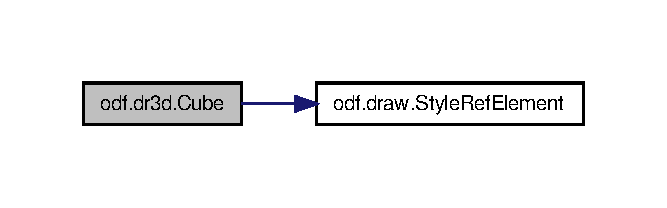
\includegraphics[width=320pt]{namespaceodf_1_1dr3d_aba28eec6f99ef3087a9eea2466d23519_cgraph}
\end{center}
\end{figure}


\hypertarget{namespaceodf_1_1dr3d_ae362ce3da2d61861bdc952e265ed2e04}{\index{odf\+::dr3d@{odf\+::dr3d}!Extrude@{Extrude}}
\index{Extrude@{Extrude}!odf\+::dr3d@{odf\+::dr3d}}
\subsubsection[{Extrude}]{\setlength{\rightskip}{0pt plus 5cm}def odf.\+dr3d.\+Extrude (
\begin{DoxyParamCaption}
\item[{}]{args}
\end{DoxyParamCaption}
)}}\label{namespaceodf_1_1dr3d_ae362ce3da2d61861bdc952e265ed2e04}


Definition at line 31 of file dr3d.\+py.



Here is the call graph for this function\+:
\nopagebreak
\begin{figure}[H]
\begin{center}
\leavevmode
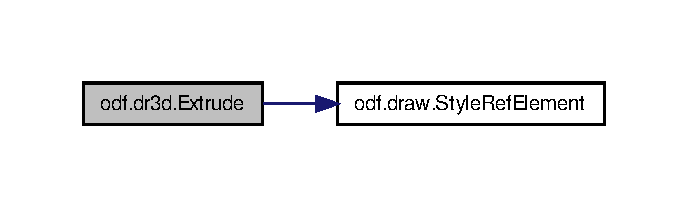
\includegraphics[width=330pt]{namespaceodf_1_1dr3d_ae362ce3da2d61861bdc952e265ed2e04_cgraph}
\end{center}
\end{figure}


\hypertarget{namespaceodf_1_1dr3d_a103936ecf1180522905dc79982c87d31}{\index{odf\+::dr3d@{odf\+::dr3d}!Light@{Light}}
\index{Light@{Light}!odf\+::dr3d@{odf\+::dr3d}}
\subsubsection[{Light}]{\setlength{\rightskip}{0pt plus 5cm}def odf.\+dr3d.\+Light (
\begin{DoxyParamCaption}
\item[{}]{Element}
\end{DoxyParamCaption}
)}}\label{namespaceodf_1_1dr3d_a103936ecf1180522905dc79982c87d31}


Definition at line 34 of file dr3d.\+py.



Here is the call graph for this function\+:
\nopagebreak
\begin{figure}[H]
\begin{center}
\leavevmode
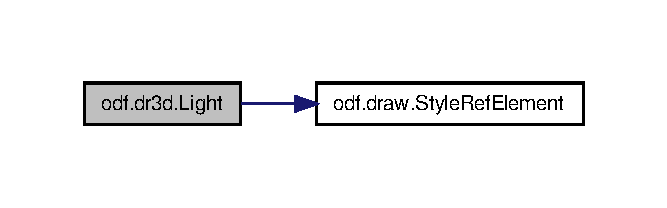
\includegraphics[width=320pt]{namespaceodf_1_1dr3d_a103936ecf1180522905dc79982c87d31_cgraph}
\end{center}
\end{figure}


\hypertarget{namespaceodf_1_1dr3d_a4f9c7c75c9b3185c3528e10166ed9b2b}{\index{odf\+::dr3d@{odf\+::dr3d}!Rotate@{Rotate}}
\index{Rotate@{Rotate}!odf\+::dr3d@{odf\+::dr3d}}
\subsubsection[{Rotate}]{\setlength{\rightskip}{0pt plus 5cm}def odf.\+dr3d.\+Rotate (
\begin{DoxyParamCaption}
\item[{}]{args}
\end{DoxyParamCaption}
)}}\label{namespaceodf_1_1dr3d_a4f9c7c75c9b3185c3528e10166ed9b2b}


Definition at line 37 of file dr3d.\+py.



Here is the call graph for this function\+:
\nopagebreak
\begin{figure}[H]
\begin{center}
\leavevmode
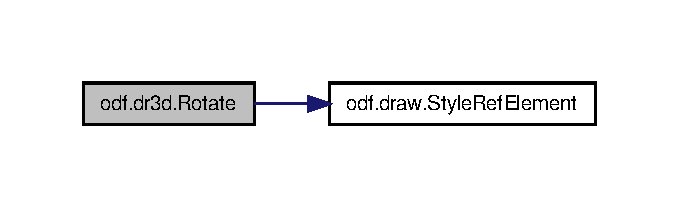
\includegraphics[width=326pt]{namespaceodf_1_1dr3d_a4f9c7c75c9b3185c3528e10166ed9b2b_cgraph}
\end{center}
\end{figure}


\hypertarget{namespaceodf_1_1dr3d_a5a8f373f91a79140287e56efd0f2c293}{\index{odf\+::dr3d@{odf\+::dr3d}!Scene@{Scene}}
\index{Scene@{Scene}!odf\+::dr3d@{odf\+::dr3d}}
\subsubsection[{Scene}]{\setlength{\rightskip}{0pt plus 5cm}def odf.\+dr3d.\+Scene (
\begin{DoxyParamCaption}
\item[{}]{args}
\end{DoxyParamCaption}
)}}\label{namespaceodf_1_1dr3d_a5a8f373f91a79140287e56efd0f2c293}


Definition at line 40 of file dr3d.\+py.



Here is the call graph for this function\+:
\nopagebreak
\begin{figure}[H]
\begin{center}
\leavevmode
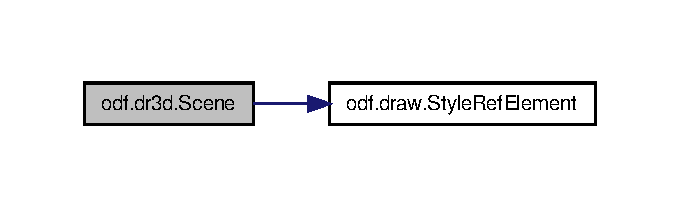
\includegraphics[width=326pt]{namespaceodf_1_1dr3d_a5a8f373f91a79140287e56efd0f2c293_cgraph}
\end{center}
\end{figure}


\hypertarget{namespaceodf_1_1dr3d_a1fec5cfe7a206d33efe637fd268ce1d7}{\index{odf\+::dr3d@{odf\+::dr3d}!Sphere@{Sphere}}
\index{Sphere@{Sphere}!odf\+::dr3d@{odf\+::dr3d}}
\subsubsection[{Sphere}]{\setlength{\rightskip}{0pt plus 5cm}def odf.\+dr3d.\+Sphere (
\begin{DoxyParamCaption}
\item[{}]{args}
\end{DoxyParamCaption}
)}}\label{namespaceodf_1_1dr3d_a1fec5cfe7a206d33efe637fd268ce1d7}


Definition at line 43 of file dr3d.\+py.



Here is the call graph for this function\+:
\nopagebreak
\begin{figure}[H]
\begin{center}
\leavevmode
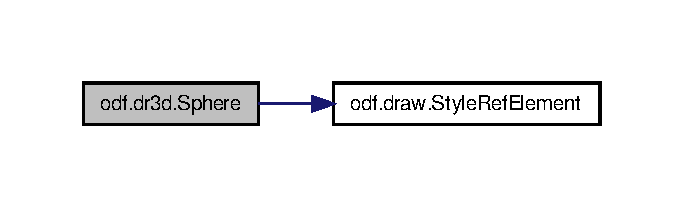
\includegraphics[width=328pt]{namespaceodf_1_1dr3d_a1fec5cfe7a206d33efe637fd268ce1d7_cgraph}
\end{center}
\end{figure}



\hypertarget{namespaceodf_1_1draw}{\section{odf.\+draw Namespace Reference}
\label{namespaceodf_1_1draw}\index{odf.\+draw@{odf.\+draw}}
}
\subsection*{Functions}
\begin{DoxyCompactItemize}
\item 
def \hyperlink{namespaceodf_1_1draw_a3370d99ab01e834591bb75a5869210eb}{Style\+Ref\+Element}
\item 
def \hyperlink{namespaceodf_1_1draw_ad32983860999b41f360b18465324e08e}{Draw\+Element}
\item 
def \hyperlink{namespaceodf_1_1draw_afd937d91013bd4294daea4ea6c654f74}{A}
\item 
def \hyperlink{namespaceodf_1_1draw_aff4b5b20eb72874d3b7c293967279e88}{Applet}
\item 
def \hyperlink{namespaceodf_1_1draw_a3052496223c87d40b76411aaa2170b04}{Area\+Circle}
\item 
def \hyperlink{namespaceodf_1_1draw_a9017e41469d2f0e3f57c27b5616269d1}{Area\+Polygon}
\item 
def \hyperlink{namespaceodf_1_1draw_a98d40da55f425f4529a672ddea027340}{Area\+Rectangle}
\item 
def \hyperlink{namespaceodf_1_1draw_a1fcf417ecc69c5f64a5825f68b356fa1}{Caption}
\item 
def \hyperlink{namespaceodf_1_1draw_ab0956530dc535c6f1776b823113c4bc0}{Circle}
\item 
def \hyperlink{namespaceodf_1_1draw_a092f2cd3049571abdfb5d6a03ab696cc}{Connector}
\item 
def \hyperlink{namespaceodf_1_1draw_a5a7cb81fbf2ab55f193f806f60f7d10a}{Contour\+Path}
\item 
def \hyperlink{namespaceodf_1_1draw_a6e5f52b95848dabe28c08801d01fac76}{Contour\+Polygon}
\item 
def \hyperlink{namespaceodf_1_1draw_a6f3480962e7b3bc1a970d6b33ba44e10}{Control}
\item 
def \hyperlink{namespaceodf_1_1draw_a8302202708fe540f98e9ad352d07cd8d}{Custom\+Shape}
\item 
def \hyperlink{namespaceodf_1_1draw_ac1020dc0376882dee7c4b45a81c659bb}{Ellipse}
\item 
def \hyperlink{namespaceodf_1_1draw_a79fef1410b20220399a8d9532b3f23ab}{Enhanced\+Geometry}
\item 
def \hyperlink{namespaceodf_1_1draw_a8019aee1cf8638aaf8e058495224e18b}{Equation}
\item 
def \hyperlink{namespaceodf_1_1draw_a7820347b2c8c35512386f5e492cedfcd}{Fill\+Image}
\item 
def \hyperlink{namespaceodf_1_1draw_a42143f3cd61ca255070b76aa0d8a60a3}{Floating\+Frame}
\item 
def \hyperlink{namespaceodf_1_1draw_a6982db25567ebf0e29f1c37e1b407908}{Frame}
\item 
def \hyperlink{namespaceodf_1_1draw_ad2abf6ab0b81e09da0eb0c06c2306f7c}{G}
\item 
def \hyperlink{namespaceodf_1_1draw_a999d7da1ea0a91f20d4128e2ac523932}{Glue\+Point}
\item 
def \hyperlink{namespaceodf_1_1draw_ac59308ebd82c72f4dc098358f6dcee3d}{Gradient}
\item 
def \hyperlink{namespaceodf_1_1draw_a569e0a30f3f44d4fc719813301a038c5}{Handle}
\item 
def \hyperlink{namespaceodf_1_1draw_a6732a23a2cfbdc0f8b06c9b14c9926c1}{Hatch}
\item 
def \hyperlink{namespaceodf_1_1draw_a61b6b6a5bb6eda79ec00a4efa1c982f0}{Image}
\item 
def \hyperlink{namespaceodf_1_1draw_a0c1d56af25f232e8b0011e0bf823fa85}{Image\+Map}
\item 
def \hyperlink{namespaceodf_1_1draw_aae9eb5ae46e536c8800b5b18a7868b19}{Layer}
\item 
def \hyperlink{namespaceodf_1_1draw_aad2a0699ae7b759c24ab1c6a25b835a7}{Layer\+Set}
\item 
def \hyperlink{namespaceodf_1_1draw_abdd7c40b2d4504744fb37e12ee393d68}{Line}
\item 
def \hyperlink{namespaceodf_1_1draw_ae9494b54e945c5cfe9dd175d89cf4b4a}{Marker}
\item 
def \hyperlink{namespaceodf_1_1draw_aaeed001f3e9662b4f06fbf1f01a120e2}{Measure}
\item 
def \hyperlink{namespaceodf_1_1draw_a522a026426f3bad7e74e09f82b3ab770}{Object}
\item 
def \hyperlink{namespaceodf_1_1draw_ac670ba8a406d2bfe044b810c0adcf1cb}{Object\+Ole}
\item 
def \hyperlink{namespaceodf_1_1draw_a398ffbd306f5b6f16b846356ffa7066e}{Opacity}
\item 
def \hyperlink{namespaceodf_1_1draw_a2cec76f7cbd3acbca5c5eba5290e5754}{Page}
\item 
def \hyperlink{namespaceodf_1_1draw_a15b1916f99b043836a0a9a2f89aac3cf}{Page\+Thumbnail}
\item 
def \hyperlink{namespaceodf_1_1draw_ae115f1ae0577c14a38cbd0a29af7d49c}{Param}
\item 
def \hyperlink{namespaceodf_1_1draw_a78e1bf674d5b1a4c0012b2f914a5be1c}{Path}
\item 
def \hyperlink{namespaceodf_1_1draw_aa5b4f851ae54c6af9db3de8c4485592b}{Plugin}
\item 
def \hyperlink{namespaceodf_1_1draw_a150f60a7954bf8079746da0f7c5c1224}{Polygon}
\item 
def \hyperlink{namespaceodf_1_1draw_a080e54252677a66c80c2c5093c094e57}{Polyline}
\item 
def \hyperlink{namespaceodf_1_1draw_aa4fd010d615a735e14c4240ec0a33e9e}{Rect}
\item 
def \hyperlink{namespaceodf_1_1draw_a2a7e04c9f2f98f894903b0b0109f4977}{Regular\+Polygon}
\item 
def \hyperlink{namespaceodf_1_1draw_aa72c3c77b8286dc168a665a6f7c8fb82}{Stroke\+Dash}
\item 
def \hyperlink{namespaceodf_1_1draw_a7cc02a01dccf5779c08f1316aff18eab}{Text\+Box}
\end{DoxyCompactItemize}


\subsection{Function Documentation}
\hypertarget{namespaceodf_1_1draw_afd937d91013bd4294daea4ea6c654f74}{\index{odf\+::draw@{odf\+::draw}!A@{A}}
\index{A@{A}!odf\+::draw@{odf\+::draw}}
\subsubsection[{A}]{\setlength{\rightskip}{0pt plus 5cm}def odf.\+draw.\+A (
\begin{DoxyParamCaption}
\item[{}]{args}
\end{DoxyParamCaption}
)}}\label{namespaceodf_1_1draw_afd937d91013bd4294daea4ea6c654f74}


Definition at line 53 of file draw.\+py.

\hypertarget{namespaceodf_1_1draw_aff4b5b20eb72874d3b7c293967279e88}{\index{odf\+::draw@{odf\+::draw}!Applet@{Applet}}
\index{Applet@{Applet}!odf\+::draw@{odf\+::draw}}
\subsubsection[{Applet}]{\setlength{\rightskip}{0pt plus 5cm}def odf.\+draw.\+Applet (
\begin{DoxyParamCaption}
\item[{}]{args}
\end{DoxyParamCaption}
)}}\label{namespaceodf_1_1draw_aff4b5b20eb72874d3b7c293967279e88}


Definition at line 57 of file draw.\+py.

\hypertarget{namespaceodf_1_1draw_a3052496223c87d40b76411aaa2170b04}{\index{odf\+::draw@{odf\+::draw}!Area\+Circle@{Area\+Circle}}
\index{Area\+Circle@{Area\+Circle}!odf\+::draw@{odf\+::draw}}
\subsubsection[{Area\+Circle}]{\setlength{\rightskip}{0pt plus 5cm}def odf.\+draw.\+Area\+Circle (
\begin{DoxyParamCaption}
\item[{}]{args}
\end{DoxyParamCaption}
)}}\label{namespaceodf_1_1draw_a3052496223c87d40b76411aaa2170b04}


Definition at line 60 of file draw.\+py.

\hypertarget{namespaceodf_1_1draw_a9017e41469d2f0e3f57c27b5616269d1}{\index{odf\+::draw@{odf\+::draw}!Area\+Polygon@{Area\+Polygon}}
\index{Area\+Polygon@{Area\+Polygon}!odf\+::draw@{odf\+::draw}}
\subsubsection[{Area\+Polygon}]{\setlength{\rightskip}{0pt plus 5cm}def odf.\+draw.\+Area\+Polygon (
\begin{DoxyParamCaption}
\item[{}]{args}
\end{DoxyParamCaption}
)}}\label{namespaceodf_1_1draw_a9017e41469d2f0e3f57c27b5616269d1}


Definition at line 63 of file draw.\+py.

\hypertarget{namespaceodf_1_1draw_a98d40da55f425f4529a672ddea027340}{\index{odf\+::draw@{odf\+::draw}!Area\+Rectangle@{Area\+Rectangle}}
\index{Area\+Rectangle@{Area\+Rectangle}!odf\+::draw@{odf\+::draw}}
\subsubsection[{Area\+Rectangle}]{\setlength{\rightskip}{0pt plus 5cm}def odf.\+draw.\+Area\+Rectangle (
\begin{DoxyParamCaption}
\item[{}]{args}
\end{DoxyParamCaption}
)}}\label{namespaceodf_1_1draw_a98d40da55f425f4529a672ddea027340}


Definition at line 66 of file draw.\+py.

\hypertarget{namespaceodf_1_1draw_a1fcf417ecc69c5f64a5825f68b356fa1}{\index{odf\+::draw@{odf\+::draw}!Caption@{Caption}}
\index{Caption@{Caption}!odf\+::draw@{odf\+::draw}}
\subsubsection[{Caption}]{\setlength{\rightskip}{0pt plus 5cm}def odf.\+draw.\+Caption (
\begin{DoxyParamCaption}
\item[{}]{args}
\end{DoxyParamCaption}
)}}\label{namespaceodf_1_1draw_a1fcf417ecc69c5f64a5825f68b356fa1}


Definition at line 69 of file draw.\+py.



Here is the call graph for this function\+:
\nopagebreak
\begin{figure}[H]
\begin{center}
\leavevmode
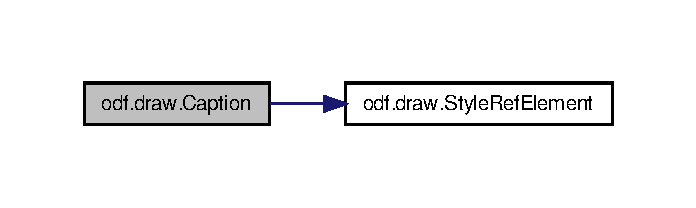
\includegraphics[width=334pt]{namespaceodf_1_1draw_a1fcf417ecc69c5f64a5825f68b356fa1_cgraph}
\end{center}
\end{figure}


\hypertarget{namespaceodf_1_1draw_ab0956530dc535c6f1776b823113c4bc0}{\index{odf\+::draw@{odf\+::draw}!Circle@{Circle}}
\index{Circle@{Circle}!odf\+::draw@{odf\+::draw}}
\subsubsection[{Circle}]{\setlength{\rightskip}{0pt plus 5cm}def odf.\+draw.\+Circle (
\begin{DoxyParamCaption}
\item[{}]{args}
\end{DoxyParamCaption}
)}}\label{namespaceodf_1_1draw_ab0956530dc535c6f1776b823113c4bc0}


Definition at line 72 of file draw.\+py.



Here is the call graph for this function\+:
\nopagebreak
\begin{figure}[H]
\begin{center}
\leavevmode
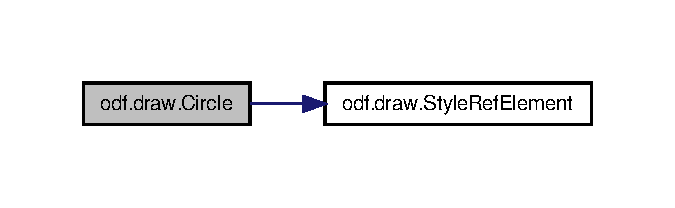
\includegraphics[width=324pt]{namespaceodf_1_1draw_ab0956530dc535c6f1776b823113c4bc0_cgraph}
\end{center}
\end{figure}


\hypertarget{namespaceodf_1_1draw_a092f2cd3049571abdfb5d6a03ab696cc}{\index{odf\+::draw@{odf\+::draw}!Connector@{Connector}}
\index{Connector@{Connector}!odf\+::draw@{odf\+::draw}}
\subsubsection[{Connector}]{\setlength{\rightskip}{0pt plus 5cm}def odf.\+draw.\+Connector (
\begin{DoxyParamCaption}
\item[{}]{args}
\end{DoxyParamCaption}
)}}\label{namespaceodf_1_1draw_a092f2cd3049571abdfb5d6a03ab696cc}


Definition at line 75 of file draw.\+py.



Here is the call graph for this function\+:
\nopagebreak
\begin{figure}[H]
\begin{center}
\leavevmode
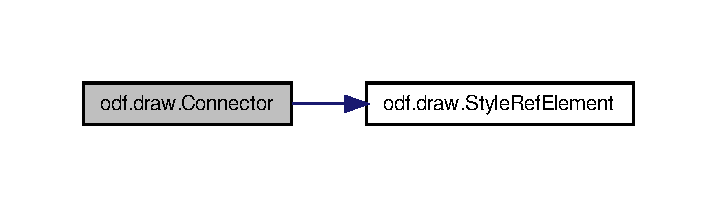
\includegraphics[width=344pt]{namespaceodf_1_1draw_a092f2cd3049571abdfb5d6a03ab696cc_cgraph}
\end{center}
\end{figure}


\hypertarget{namespaceodf_1_1draw_a5a7cb81fbf2ab55f193f806f60f7d10a}{\index{odf\+::draw@{odf\+::draw}!Contour\+Path@{Contour\+Path}}
\index{Contour\+Path@{Contour\+Path}!odf\+::draw@{odf\+::draw}}
\subsubsection[{Contour\+Path}]{\setlength{\rightskip}{0pt plus 5cm}def odf.\+draw.\+Contour\+Path (
\begin{DoxyParamCaption}
\item[{}]{args}
\end{DoxyParamCaption}
)}}\label{namespaceodf_1_1draw_a5a7cb81fbf2ab55f193f806f60f7d10a}


Definition at line 78 of file draw.\+py.

\hypertarget{namespaceodf_1_1draw_a6e5f52b95848dabe28c08801d01fac76}{\index{odf\+::draw@{odf\+::draw}!Contour\+Polygon@{Contour\+Polygon}}
\index{Contour\+Polygon@{Contour\+Polygon}!odf\+::draw@{odf\+::draw}}
\subsubsection[{Contour\+Polygon}]{\setlength{\rightskip}{0pt plus 5cm}def odf.\+draw.\+Contour\+Polygon (
\begin{DoxyParamCaption}
\item[{}]{args}
\end{DoxyParamCaption}
)}}\label{namespaceodf_1_1draw_a6e5f52b95848dabe28c08801d01fac76}


Definition at line 81 of file draw.\+py.

\hypertarget{namespaceodf_1_1draw_a6f3480962e7b3bc1a970d6b33ba44e10}{\index{odf\+::draw@{odf\+::draw}!Control@{Control}}
\index{Control@{Control}!odf\+::draw@{odf\+::draw}}
\subsubsection[{Control}]{\setlength{\rightskip}{0pt plus 5cm}def odf.\+draw.\+Control (
\begin{DoxyParamCaption}
\item[{}]{args}
\end{DoxyParamCaption}
)}}\label{namespaceodf_1_1draw_a6f3480962e7b3bc1a970d6b33ba44e10}


Definition at line 84 of file draw.\+py.



Here is the call graph for this function\+:
\nopagebreak
\begin{figure}[H]
\begin{center}
\leavevmode
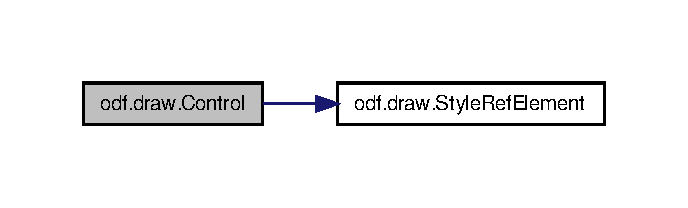
\includegraphics[width=330pt]{namespaceodf_1_1draw_a6f3480962e7b3bc1a970d6b33ba44e10_cgraph}
\end{center}
\end{figure}


\hypertarget{namespaceodf_1_1draw_a8302202708fe540f98e9ad352d07cd8d}{\index{odf\+::draw@{odf\+::draw}!Custom\+Shape@{Custom\+Shape}}
\index{Custom\+Shape@{Custom\+Shape}!odf\+::draw@{odf\+::draw}}
\subsubsection[{Custom\+Shape}]{\setlength{\rightskip}{0pt plus 5cm}def odf.\+draw.\+Custom\+Shape (
\begin{DoxyParamCaption}
\item[{}]{args}
\end{DoxyParamCaption}
)}}\label{namespaceodf_1_1draw_a8302202708fe540f98e9ad352d07cd8d}


Definition at line 87 of file draw.\+py.



Here is the call graph for this function\+:
\nopagebreak
\begin{figure}[H]
\begin{center}
\leavevmode
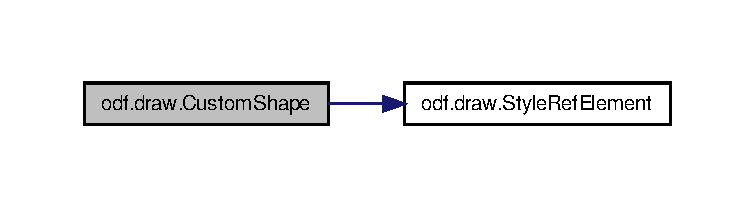
\includegraphics[width=350pt]{namespaceodf_1_1draw_a8302202708fe540f98e9ad352d07cd8d_cgraph}
\end{center}
\end{figure}


\hypertarget{namespaceodf_1_1draw_ad32983860999b41f360b18465324e08e}{\index{odf\+::draw@{odf\+::draw}!Draw\+Element@{Draw\+Element}}
\index{Draw\+Element@{Draw\+Element}!odf\+::draw@{odf\+::draw}}
\subsubsection[{Draw\+Element}]{\setlength{\rightskip}{0pt plus 5cm}def odf.\+draw.\+Draw\+Element (
\begin{DoxyParamCaption}
\item[{}]{name = {\ttfamily None}, }
\item[{}]{args}
\end{DoxyParamCaption}
)}}\label{namespaceodf_1_1draw_ad32983860999b41f360b18465324e08e}


Definition at line 46 of file draw.\+py.



Here is the caller graph for this function\+:
\nopagebreak
\begin{figure}[H]
\begin{center}
\leavevmode
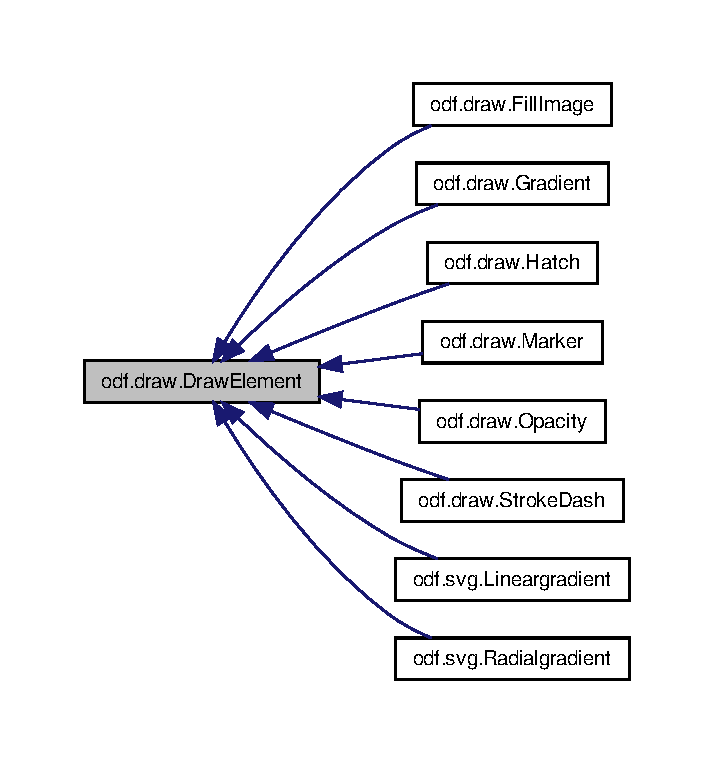
\includegraphics[width=342pt]{namespaceodf_1_1draw_ad32983860999b41f360b18465324e08e_icgraph}
\end{center}
\end{figure}


\hypertarget{namespaceodf_1_1draw_ac1020dc0376882dee7c4b45a81c659bb}{\index{odf\+::draw@{odf\+::draw}!Ellipse@{Ellipse}}
\index{Ellipse@{Ellipse}!odf\+::draw@{odf\+::draw}}
\subsubsection[{Ellipse}]{\setlength{\rightskip}{0pt plus 5cm}def odf.\+draw.\+Ellipse (
\begin{DoxyParamCaption}
\item[{}]{args}
\end{DoxyParamCaption}
)}}\label{namespaceodf_1_1draw_ac1020dc0376882dee7c4b45a81c659bb}


Definition at line 90 of file draw.\+py.



Here is the call graph for this function\+:
\nopagebreak
\begin{figure}[H]
\begin{center}
\leavevmode
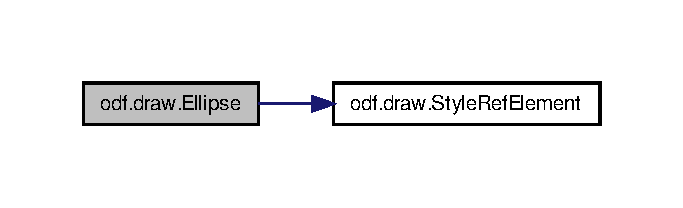
\includegraphics[width=328pt]{namespaceodf_1_1draw_ac1020dc0376882dee7c4b45a81c659bb_cgraph}
\end{center}
\end{figure}


\hypertarget{namespaceodf_1_1draw_a79fef1410b20220399a8d9532b3f23ab}{\index{odf\+::draw@{odf\+::draw}!Enhanced\+Geometry@{Enhanced\+Geometry}}
\index{Enhanced\+Geometry@{Enhanced\+Geometry}!odf\+::draw@{odf\+::draw}}
\subsubsection[{Enhanced\+Geometry}]{\setlength{\rightskip}{0pt plus 5cm}def odf.\+draw.\+Enhanced\+Geometry (
\begin{DoxyParamCaption}
\item[{}]{args}
\end{DoxyParamCaption}
)}}\label{namespaceodf_1_1draw_a79fef1410b20220399a8d9532b3f23ab}


Definition at line 93 of file draw.\+py.

\hypertarget{namespaceodf_1_1draw_a8019aee1cf8638aaf8e058495224e18b}{\index{odf\+::draw@{odf\+::draw}!Equation@{Equation}}
\index{Equation@{Equation}!odf\+::draw@{odf\+::draw}}
\subsubsection[{Equation}]{\setlength{\rightskip}{0pt plus 5cm}def odf.\+draw.\+Equation (
\begin{DoxyParamCaption}
\item[{}]{args}
\end{DoxyParamCaption}
)}}\label{namespaceodf_1_1draw_a8019aee1cf8638aaf8e058495224e18b}


Definition at line 96 of file draw.\+py.

\hypertarget{namespaceodf_1_1draw_a7820347b2c8c35512386f5e492cedfcd}{\index{odf\+::draw@{odf\+::draw}!Fill\+Image@{Fill\+Image}}
\index{Fill\+Image@{Fill\+Image}!odf\+::draw@{odf\+::draw}}
\subsubsection[{Fill\+Image}]{\setlength{\rightskip}{0pt plus 5cm}def odf.\+draw.\+Fill\+Image (
\begin{DoxyParamCaption}
\item[{}]{args}
\end{DoxyParamCaption}
)}}\label{namespaceodf_1_1draw_a7820347b2c8c35512386f5e492cedfcd}


Definition at line 99 of file draw.\+py.



Here is the call graph for this function\+:
\nopagebreak
\begin{figure}[H]
\begin{center}
\leavevmode
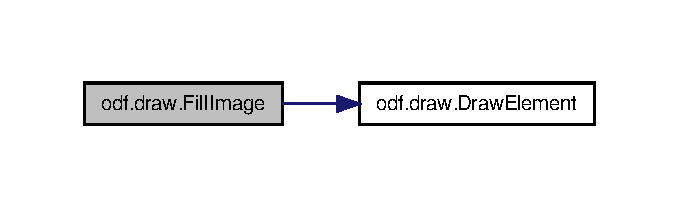
\includegraphics[width=326pt]{namespaceodf_1_1draw_a7820347b2c8c35512386f5e492cedfcd_cgraph}
\end{center}
\end{figure}


\hypertarget{namespaceodf_1_1draw_a42143f3cd61ca255070b76aa0d8a60a3}{\index{odf\+::draw@{odf\+::draw}!Floating\+Frame@{Floating\+Frame}}
\index{Floating\+Frame@{Floating\+Frame}!odf\+::draw@{odf\+::draw}}
\subsubsection[{Floating\+Frame}]{\setlength{\rightskip}{0pt plus 5cm}def odf.\+draw.\+Floating\+Frame (
\begin{DoxyParamCaption}
\item[{}]{args}
\end{DoxyParamCaption}
)}}\label{namespaceodf_1_1draw_a42143f3cd61ca255070b76aa0d8a60a3}


Definition at line 103 of file draw.\+py.

\hypertarget{namespaceodf_1_1draw_a6982db25567ebf0e29f1c37e1b407908}{\index{odf\+::draw@{odf\+::draw}!Frame@{Frame}}
\index{Frame@{Frame}!odf\+::draw@{odf\+::draw}}
\subsubsection[{Frame}]{\setlength{\rightskip}{0pt plus 5cm}def odf.\+draw.\+Frame (
\begin{DoxyParamCaption}
\item[{}]{args}
\end{DoxyParamCaption}
)}}\label{namespaceodf_1_1draw_a6982db25567ebf0e29f1c37e1b407908}


Definition at line 107 of file draw.\+py.



Here is the call graph for this function\+:
\nopagebreak
\begin{figure}[H]
\begin{center}
\leavevmode
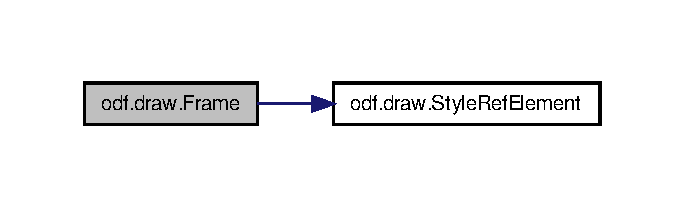
\includegraphics[width=328pt]{namespaceodf_1_1draw_a6982db25567ebf0e29f1c37e1b407908_cgraph}
\end{center}
\end{figure}


\hypertarget{namespaceodf_1_1draw_ad2abf6ab0b81e09da0eb0c06c2306f7c}{\index{odf\+::draw@{odf\+::draw}!G@{G}}
\index{G@{G}!odf\+::draw@{odf\+::draw}}
\subsubsection[{G}]{\setlength{\rightskip}{0pt plus 5cm}def odf.\+draw.\+G (
\begin{DoxyParamCaption}
\item[{}]{args}
\end{DoxyParamCaption}
)}}\label{namespaceodf_1_1draw_ad2abf6ab0b81e09da0eb0c06c2306f7c}


Definition at line 110 of file draw.\+py.



Here is the call graph for this function\+:
\nopagebreak
\begin{figure}[H]
\begin{center}
\leavevmode
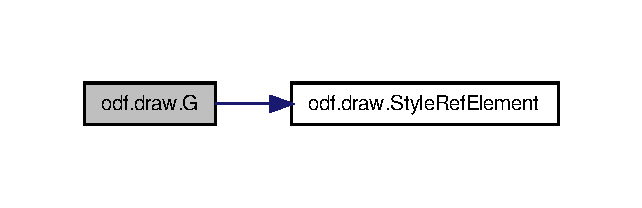
\includegraphics[width=308pt]{namespaceodf_1_1draw_ad2abf6ab0b81e09da0eb0c06c2306f7c_cgraph}
\end{center}
\end{figure}


\hypertarget{namespaceodf_1_1draw_a999d7da1ea0a91f20d4128e2ac523932}{\index{odf\+::draw@{odf\+::draw}!Glue\+Point@{Glue\+Point}}
\index{Glue\+Point@{Glue\+Point}!odf\+::draw@{odf\+::draw}}
\subsubsection[{Glue\+Point}]{\setlength{\rightskip}{0pt plus 5cm}def odf.\+draw.\+Glue\+Point (
\begin{DoxyParamCaption}
\item[{}]{args}
\end{DoxyParamCaption}
)}}\label{namespaceodf_1_1draw_a999d7da1ea0a91f20d4128e2ac523932}


Definition at line 113 of file draw.\+py.

\hypertarget{namespaceodf_1_1draw_ac59308ebd82c72f4dc098358f6dcee3d}{\index{odf\+::draw@{odf\+::draw}!Gradient@{Gradient}}
\index{Gradient@{Gradient}!odf\+::draw@{odf\+::draw}}
\subsubsection[{Gradient}]{\setlength{\rightskip}{0pt plus 5cm}def odf.\+draw.\+Gradient (
\begin{DoxyParamCaption}
\item[{}]{args}
\end{DoxyParamCaption}
)}}\label{namespaceodf_1_1draw_ac59308ebd82c72f4dc098358f6dcee3d}


Definition at line 116 of file draw.\+py.



Here is the call graph for this function\+:
\nopagebreak
\begin{figure}[H]
\begin{center}
\leavevmode
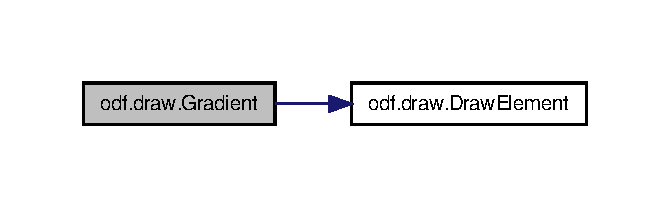
\includegraphics[width=322pt]{namespaceodf_1_1draw_ac59308ebd82c72f4dc098358f6dcee3d_cgraph}
\end{center}
\end{figure}


\hypertarget{namespaceodf_1_1draw_a569e0a30f3f44d4fc719813301a038c5}{\index{odf\+::draw@{odf\+::draw}!Handle@{Handle}}
\index{Handle@{Handle}!odf\+::draw@{odf\+::draw}}
\subsubsection[{Handle}]{\setlength{\rightskip}{0pt plus 5cm}def odf.\+draw.\+Handle (
\begin{DoxyParamCaption}
\item[{}]{args}
\end{DoxyParamCaption}
)}}\label{namespaceodf_1_1draw_a569e0a30f3f44d4fc719813301a038c5}


Definition at line 119 of file draw.\+py.

\hypertarget{namespaceodf_1_1draw_a6732a23a2cfbdc0f8b06c9b14c9926c1}{\index{odf\+::draw@{odf\+::draw}!Hatch@{Hatch}}
\index{Hatch@{Hatch}!odf\+::draw@{odf\+::draw}}
\subsubsection[{Hatch}]{\setlength{\rightskip}{0pt plus 5cm}def odf.\+draw.\+Hatch (
\begin{DoxyParamCaption}
\item[{}]{args}
\end{DoxyParamCaption}
)}}\label{namespaceodf_1_1draw_a6732a23a2cfbdc0f8b06c9b14c9926c1}


Definition at line 122 of file draw.\+py.



Here is the call graph for this function\+:
\nopagebreak
\begin{figure}[H]
\begin{center}
\leavevmode
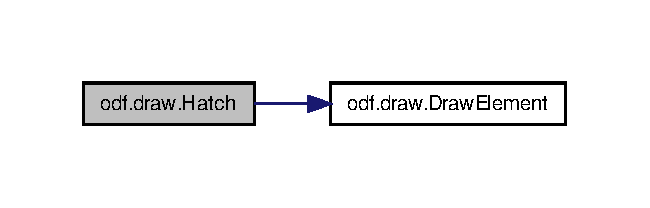
\includegraphics[width=312pt]{namespaceodf_1_1draw_a6732a23a2cfbdc0f8b06c9b14c9926c1_cgraph}
\end{center}
\end{figure}


\hypertarget{namespaceodf_1_1draw_a61b6b6a5bb6eda79ec00a4efa1c982f0}{\index{odf\+::draw@{odf\+::draw}!Image@{Image}}
\index{Image@{Image}!odf\+::draw@{odf\+::draw}}
\subsubsection[{Image}]{\setlength{\rightskip}{0pt plus 5cm}def odf.\+draw.\+Image (
\begin{DoxyParamCaption}
\item[{}]{args}
\end{DoxyParamCaption}
)}}\label{namespaceodf_1_1draw_a61b6b6a5bb6eda79ec00a4efa1c982f0}


Definition at line 125 of file draw.\+py.



Here is the caller graph for this function\+:
\nopagebreak
\begin{figure}[H]
\begin{center}
\leavevmode
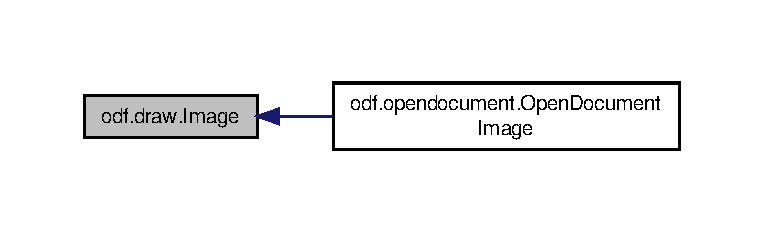
\includegraphics[width=350pt]{namespaceodf_1_1draw_a61b6b6a5bb6eda79ec00a4efa1c982f0_icgraph}
\end{center}
\end{figure}


\hypertarget{namespaceodf_1_1draw_a0c1d56af25f232e8b0011e0bf823fa85}{\index{odf\+::draw@{odf\+::draw}!Image\+Map@{Image\+Map}}
\index{Image\+Map@{Image\+Map}!odf\+::draw@{odf\+::draw}}
\subsubsection[{Image\+Map}]{\setlength{\rightskip}{0pt plus 5cm}def odf.\+draw.\+Image\+Map (
\begin{DoxyParamCaption}
\item[{}]{args}
\end{DoxyParamCaption}
)}}\label{namespaceodf_1_1draw_a0c1d56af25f232e8b0011e0bf823fa85}


Definition at line 128 of file draw.\+py.

\hypertarget{namespaceodf_1_1draw_aae9eb5ae46e536c8800b5b18a7868b19}{\index{odf\+::draw@{odf\+::draw}!Layer@{Layer}}
\index{Layer@{Layer}!odf\+::draw@{odf\+::draw}}
\subsubsection[{Layer}]{\setlength{\rightskip}{0pt plus 5cm}def odf.\+draw.\+Layer (
\begin{DoxyParamCaption}
\item[{}]{args}
\end{DoxyParamCaption}
)}}\label{namespaceodf_1_1draw_aae9eb5ae46e536c8800b5b18a7868b19}


Definition at line 131 of file draw.\+py.

\hypertarget{namespaceodf_1_1draw_aad2a0699ae7b759c24ab1c6a25b835a7}{\index{odf\+::draw@{odf\+::draw}!Layer\+Set@{Layer\+Set}}
\index{Layer\+Set@{Layer\+Set}!odf\+::draw@{odf\+::draw}}
\subsubsection[{Layer\+Set}]{\setlength{\rightskip}{0pt plus 5cm}def odf.\+draw.\+Layer\+Set (
\begin{DoxyParamCaption}
\item[{}]{args}
\end{DoxyParamCaption}
)}}\label{namespaceodf_1_1draw_aad2a0699ae7b759c24ab1c6a25b835a7}


Definition at line 134 of file draw.\+py.

\hypertarget{namespaceodf_1_1draw_abdd7c40b2d4504744fb37e12ee393d68}{\index{odf\+::draw@{odf\+::draw}!Line@{Line}}
\index{Line@{Line}!odf\+::draw@{odf\+::draw}}
\subsubsection[{Line}]{\setlength{\rightskip}{0pt plus 5cm}def odf.\+draw.\+Line (
\begin{DoxyParamCaption}
\item[{}]{args}
\end{DoxyParamCaption}
)}}\label{namespaceodf_1_1draw_abdd7c40b2d4504744fb37e12ee393d68}


Definition at line 137 of file draw.\+py.



Here is the call graph for this function\+:
\nopagebreak
\begin{figure}[H]
\begin{center}
\leavevmode
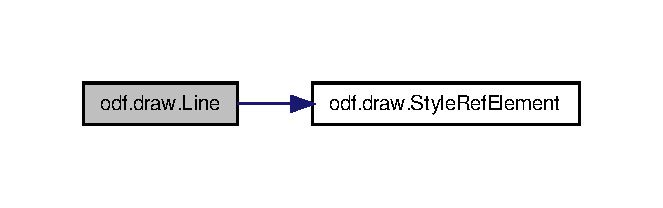
\includegraphics[width=318pt]{namespaceodf_1_1draw_abdd7c40b2d4504744fb37e12ee393d68_cgraph}
\end{center}
\end{figure}


\hypertarget{namespaceodf_1_1draw_ae9494b54e945c5cfe9dd175d89cf4b4a}{\index{odf\+::draw@{odf\+::draw}!Marker@{Marker}}
\index{Marker@{Marker}!odf\+::draw@{odf\+::draw}}
\subsubsection[{Marker}]{\setlength{\rightskip}{0pt plus 5cm}def odf.\+draw.\+Marker (
\begin{DoxyParamCaption}
\item[{}]{args}
\end{DoxyParamCaption}
)}}\label{namespaceodf_1_1draw_ae9494b54e945c5cfe9dd175d89cf4b4a}


Definition at line 140 of file draw.\+py.



Here is the call graph for this function\+:
\nopagebreak
\begin{figure}[H]
\begin{center}
\leavevmode
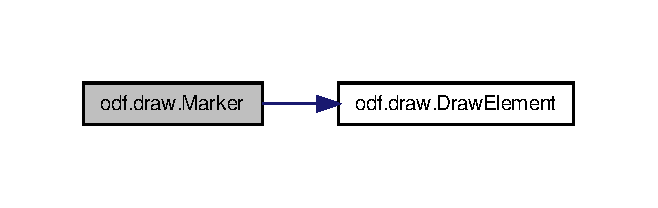
\includegraphics[width=316pt]{namespaceodf_1_1draw_ae9494b54e945c5cfe9dd175d89cf4b4a_cgraph}
\end{center}
\end{figure}


\hypertarget{namespaceodf_1_1draw_aaeed001f3e9662b4f06fbf1f01a120e2}{\index{odf\+::draw@{odf\+::draw}!Measure@{Measure}}
\index{Measure@{Measure}!odf\+::draw@{odf\+::draw}}
\subsubsection[{Measure}]{\setlength{\rightskip}{0pt plus 5cm}def odf.\+draw.\+Measure (
\begin{DoxyParamCaption}
\item[{}]{args}
\end{DoxyParamCaption}
)}}\label{namespaceodf_1_1draw_aaeed001f3e9662b4f06fbf1f01a120e2}


Definition at line 143 of file draw.\+py.



Here is the call graph for this function\+:
\nopagebreak
\begin{figure}[H]
\begin{center}
\leavevmode
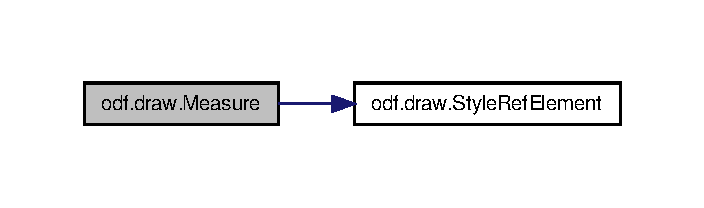
\includegraphics[width=338pt]{namespaceodf_1_1draw_aaeed001f3e9662b4f06fbf1f01a120e2_cgraph}
\end{center}
\end{figure}


\hypertarget{namespaceodf_1_1draw_a522a026426f3bad7e74e09f82b3ab770}{\index{odf\+::draw@{odf\+::draw}!Object@{Object}}
\index{Object@{Object}!odf\+::draw@{odf\+::draw}}
\subsubsection[{Object}]{\setlength{\rightskip}{0pt plus 5cm}def odf.\+draw.\+Object (
\begin{DoxyParamCaption}
\item[{}]{args}
\end{DoxyParamCaption}
)}}\label{namespaceodf_1_1draw_a522a026426f3bad7e74e09f82b3ab770}


Definition at line 146 of file draw.\+py.

\hypertarget{namespaceodf_1_1draw_ac670ba8a406d2bfe044b810c0adcf1cb}{\index{odf\+::draw@{odf\+::draw}!Object\+Ole@{Object\+Ole}}
\index{Object\+Ole@{Object\+Ole}!odf\+::draw@{odf\+::draw}}
\subsubsection[{Object\+Ole}]{\setlength{\rightskip}{0pt plus 5cm}def odf.\+draw.\+Object\+Ole (
\begin{DoxyParamCaption}
\item[{}]{args}
\end{DoxyParamCaption}
)}}\label{namespaceodf_1_1draw_ac670ba8a406d2bfe044b810c0adcf1cb}


Definition at line 149 of file draw.\+py.

\hypertarget{namespaceodf_1_1draw_a398ffbd306f5b6f16b846356ffa7066e}{\index{odf\+::draw@{odf\+::draw}!Opacity@{Opacity}}
\index{Opacity@{Opacity}!odf\+::draw@{odf\+::draw}}
\subsubsection[{Opacity}]{\setlength{\rightskip}{0pt plus 5cm}def odf.\+draw.\+Opacity (
\begin{DoxyParamCaption}
\item[{}]{args}
\end{DoxyParamCaption}
)}}\label{namespaceodf_1_1draw_a398ffbd306f5b6f16b846356ffa7066e}


Definition at line 152 of file draw.\+py.



Here is the call graph for this function\+:
\nopagebreak
\begin{figure}[H]
\begin{center}
\leavevmode
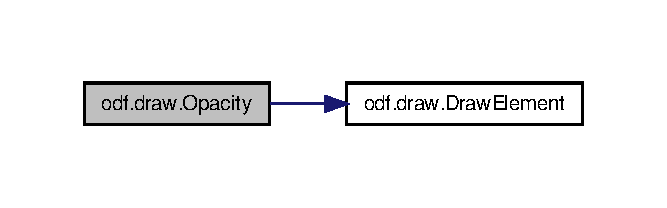
\includegraphics[width=320pt]{namespaceodf_1_1draw_a398ffbd306f5b6f16b846356ffa7066e_cgraph}
\end{center}
\end{figure}


\hypertarget{namespaceodf_1_1draw_a2cec76f7cbd3acbca5c5eba5290e5754}{\index{odf\+::draw@{odf\+::draw}!Page@{Page}}
\index{Page@{Page}!odf\+::draw@{odf\+::draw}}
\subsubsection[{Page}]{\setlength{\rightskip}{0pt plus 5cm}def odf.\+draw.\+Page (
\begin{DoxyParamCaption}
\item[{}]{args}
\end{DoxyParamCaption}
)}}\label{namespaceodf_1_1draw_a2cec76f7cbd3acbca5c5eba5290e5754}


Definition at line 155 of file draw.\+py.

\hypertarget{namespaceodf_1_1draw_a15b1916f99b043836a0a9a2f89aac3cf}{\index{odf\+::draw@{odf\+::draw}!Page\+Thumbnail@{Page\+Thumbnail}}
\index{Page\+Thumbnail@{Page\+Thumbnail}!odf\+::draw@{odf\+::draw}}
\subsubsection[{Page\+Thumbnail}]{\setlength{\rightskip}{0pt plus 5cm}def odf.\+draw.\+Page\+Thumbnail (
\begin{DoxyParamCaption}
\item[{}]{args}
\end{DoxyParamCaption}
)}}\label{namespaceodf_1_1draw_a15b1916f99b043836a0a9a2f89aac3cf}


Definition at line 158 of file draw.\+py.



Here is the call graph for this function\+:
\nopagebreak
\begin{figure}[H]
\begin{center}
\leavevmode
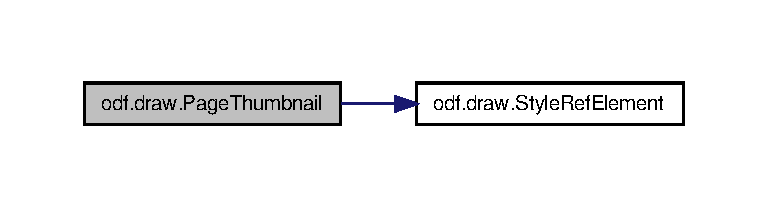
\includegraphics[width=350pt]{namespaceodf_1_1draw_a15b1916f99b043836a0a9a2f89aac3cf_cgraph}
\end{center}
\end{figure}


\hypertarget{namespaceodf_1_1draw_ae115f1ae0577c14a38cbd0a29af7d49c}{\index{odf\+::draw@{odf\+::draw}!Param@{Param}}
\index{Param@{Param}!odf\+::draw@{odf\+::draw}}
\subsubsection[{Param}]{\setlength{\rightskip}{0pt plus 5cm}def odf.\+draw.\+Param (
\begin{DoxyParamCaption}
\item[{}]{args}
\end{DoxyParamCaption}
)}}\label{namespaceodf_1_1draw_ae115f1ae0577c14a38cbd0a29af7d49c}


Definition at line 161 of file draw.\+py.

\hypertarget{namespaceodf_1_1draw_a78e1bf674d5b1a4c0012b2f914a5be1c}{\index{odf\+::draw@{odf\+::draw}!Path@{Path}}
\index{Path@{Path}!odf\+::draw@{odf\+::draw}}
\subsubsection[{Path}]{\setlength{\rightskip}{0pt plus 5cm}def odf.\+draw.\+Path (
\begin{DoxyParamCaption}
\item[{}]{args}
\end{DoxyParamCaption}
)}}\label{namespaceodf_1_1draw_a78e1bf674d5b1a4c0012b2f914a5be1c}


Definition at line 164 of file draw.\+py.



Here is the call graph for this function\+:
\nopagebreak
\begin{figure}[H]
\begin{center}
\leavevmode
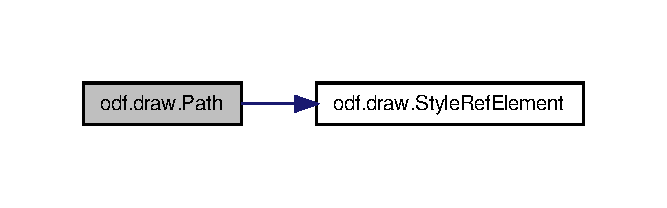
\includegraphics[width=320pt]{namespaceodf_1_1draw_a78e1bf674d5b1a4c0012b2f914a5be1c_cgraph}
\end{center}
\end{figure}


\hypertarget{namespaceodf_1_1draw_aa5b4f851ae54c6af9db3de8c4485592b}{\index{odf\+::draw@{odf\+::draw}!Plugin@{Plugin}}
\index{Plugin@{Plugin}!odf\+::draw@{odf\+::draw}}
\subsubsection[{Plugin}]{\setlength{\rightskip}{0pt plus 5cm}def odf.\+draw.\+Plugin (
\begin{DoxyParamCaption}
\item[{}]{args}
\end{DoxyParamCaption}
)}}\label{namespaceodf_1_1draw_aa5b4f851ae54c6af9db3de8c4485592b}


Definition at line 167 of file draw.\+py.

\hypertarget{namespaceodf_1_1draw_a150f60a7954bf8079746da0f7c5c1224}{\index{odf\+::draw@{odf\+::draw}!Polygon@{Polygon}}
\index{Polygon@{Polygon}!odf\+::draw@{odf\+::draw}}
\subsubsection[{Polygon}]{\setlength{\rightskip}{0pt plus 5cm}def odf.\+draw.\+Polygon (
\begin{DoxyParamCaption}
\item[{}]{args}
\end{DoxyParamCaption}
)}}\label{namespaceodf_1_1draw_a150f60a7954bf8079746da0f7c5c1224}


Definition at line 171 of file draw.\+py.



Here is the call graph for this function\+:
\nopagebreak
\begin{figure}[H]
\begin{center}
\leavevmode
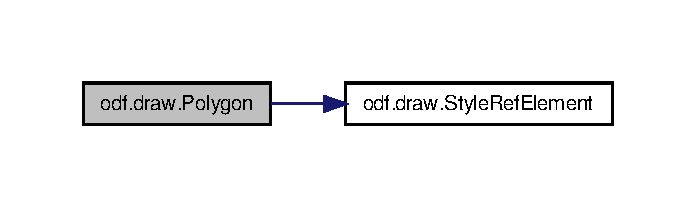
\includegraphics[width=334pt]{namespaceodf_1_1draw_a150f60a7954bf8079746da0f7c5c1224_cgraph}
\end{center}
\end{figure}


\hypertarget{namespaceodf_1_1draw_a080e54252677a66c80c2c5093c094e57}{\index{odf\+::draw@{odf\+::draw}!Polyline@{Polyline}}
\index{Polyline@{Polyline}!odf\+::draw@{odf\+::draw}}
\subsubsection[{Polyline}]{\setlength{\rightskip}{0pt plus 5cm}def odf.\+draw.\+Polyline (
\begin{DoxyParamCaption}
\item[{}]{args}
\end{DoxyParamCaption}
)}}\label{namespaceodf_1_1draw_a080e54252677a66c80c2c5093c094e57}


Definition at line 174 of file draw.\+py.



Here is the call graph for this function\+:
\nopagebreak
\begin{figure}[H]
\begin{center}
\leavevmode
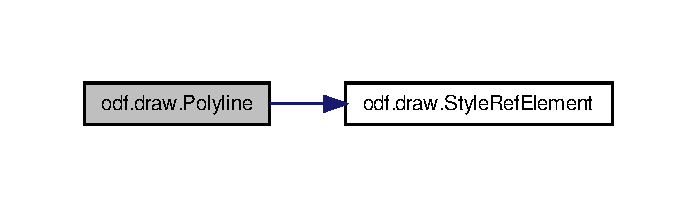
\includegraphics[width=334pt]{namespaceodf_1_1draw_a080e54252677a66c80c2c5093c094e57_cgraph}
\end{center}
\end{figure}


\hypertarget{namespaceodf_1_1draw_aa4fd010d615a735e14c4240ec0a33e9e}{\index{odf\+::draw@{odf\+::draw}!Rect@{Rect}}
\index{Rect@{Rect}!odf\+::draw@{odf\+::draw}}
\subsubsection[{Rect}]{\setlength{\rightskip}{0pt plus 5cm}def odf.\+draw.\+Rect (
\begin{DoxyParamCaption}
\item[{}]{args}
\end{DoxyParamCaption}
)}}\label{namespaceodf_1_1draw_aa4fd010d615a735e14c4240ec0a33e9e}


Definition at line 177 of file draw.\+py.



Here is the call graph for this function\+:
\nopagebreak
\begin{figure}[H]
\begin{center}
\leavevmode
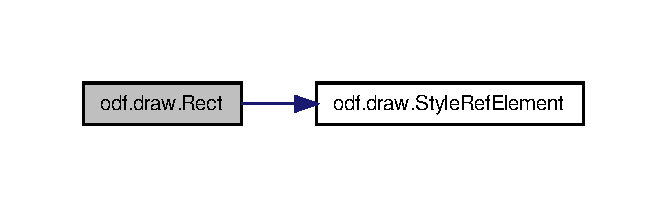
\includegraphics[width=320pt]{namespaceodf_1_1draw_aa4fd010d615a735e14c4240ec0a33e9e_cgraph}
\end{center}
\end{figure}


\hypertarget{namespaceodf_1_1draw_a2a7e04c9f2f98f894903b0b0109f4977}{\index{odf\+::draw@{odf\+::draw}!Regular\+Polygon@{Regular\+Polygon}}
\index{Regular\+Polygon@{Regular\+Polygon}!odf\+::draw@{odf\+::draw}}
\subsubsection[{Regular\+Polygon}]{\setlength{\rightskip}{0pt plus 5cm}def odf.\+draw.\+Regular\+Polygon (
\begin{DoxyParamCaption}
\item[{}]{args}
\end{DoxyParamCaption}
)}}\label{namespaceodf_1_1draw_a2a7e04c9f2f98f894903b0b0109f4977}


Definition at line 180 of file draw.\+py.



Here is the call graph for this function\+:
\nopagebreak
\begin{figure}[H]
\begin{center}
\leavevmode
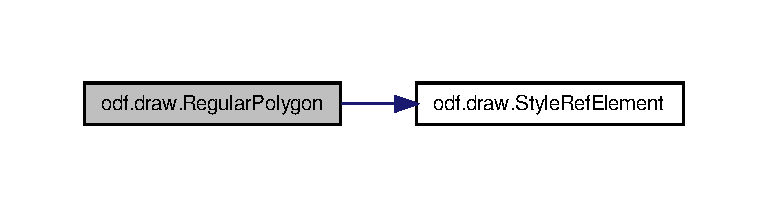
\includegraphics[width=350pt]{namespaceodf_1_1draw_a2a7e04c9f2f98f894903b0b0109f4977_cgraph}
\end{center}
\end{figure}


\hypertarget{namespaceodf_1_1draw_aa72c3c77b8286dc168a665a6f7c8fb82}{\index{odf\+::draw@{odf\+::draw}!Stroke\+Dash@{Stroke\+Dash}}
\index{Stroke\+Dash@{Stroke\+Dash}!odf\+::draw@{odf\+::draw}}
\subsubsection[{Stroke\+Dash}]{\setlength{\rightskip}{0pt plus 5cm}def odf.\+draw.\+Stroke\+Dash (
\begin{DoxyParamCaption}
\item[{}]{args}
\end{DoxyParamCaption}
)}}\label{namespaceodf_1_1draw_aa72c3c77b8286dc168a665a6f7c8fb82}


Definition at line 183 of file draw.\+py.



Here is the call graph for this function\+:
\nopagebreak
\begin{figure}[H]
\begin{center}
\leavevmode
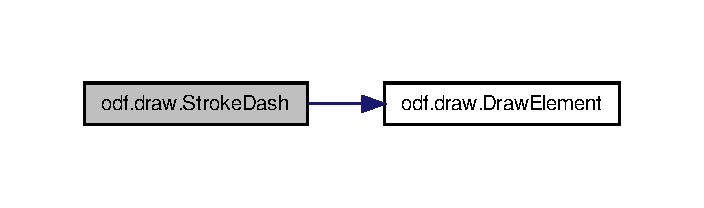
\includegraphics[width=338pt]{namespaceodf_1_1draw_aa72c3c77b8286dc168a665a6f7c8fb82_cgraph}
\end{center}
\end{figure}


\hypertarget{namespaceodf_1_1draw_a3370d99ab01e834591bb75a5869210eb}{\index{odf\+::draw@{odf\+::draw}!Style\+Ref\+Element@{Style\+Ref\+Element}}
\index{Style\+Ref\+Element@{Style\+Ref\+Element}!odf\+::draw@{odf\+::draw}}
\subsubsection[{Style\+Ref\+Element}]{\setlength{\rightskip}{0pt plus 5cm}def odf.\+draw.\+Style\+Ref\+Element (
\begin{DoxyParamCaption}
\item[{}]{stylename = {\ttfamily None}, }
\item[{}]{classnames = {\ttfamily None}, }
\item[{}]{args}
\end{DoxyParamCaption}
)}}\label{namespaceodf_1_1draw_a3370d99ab01e834591bb75a5869210eb}


Definition at line 26 of file draw.\+py.



Here is the caller graph for this function\+:
\nopagebreak
\begin{figure}[H]
\begin{center}
\leavevmode
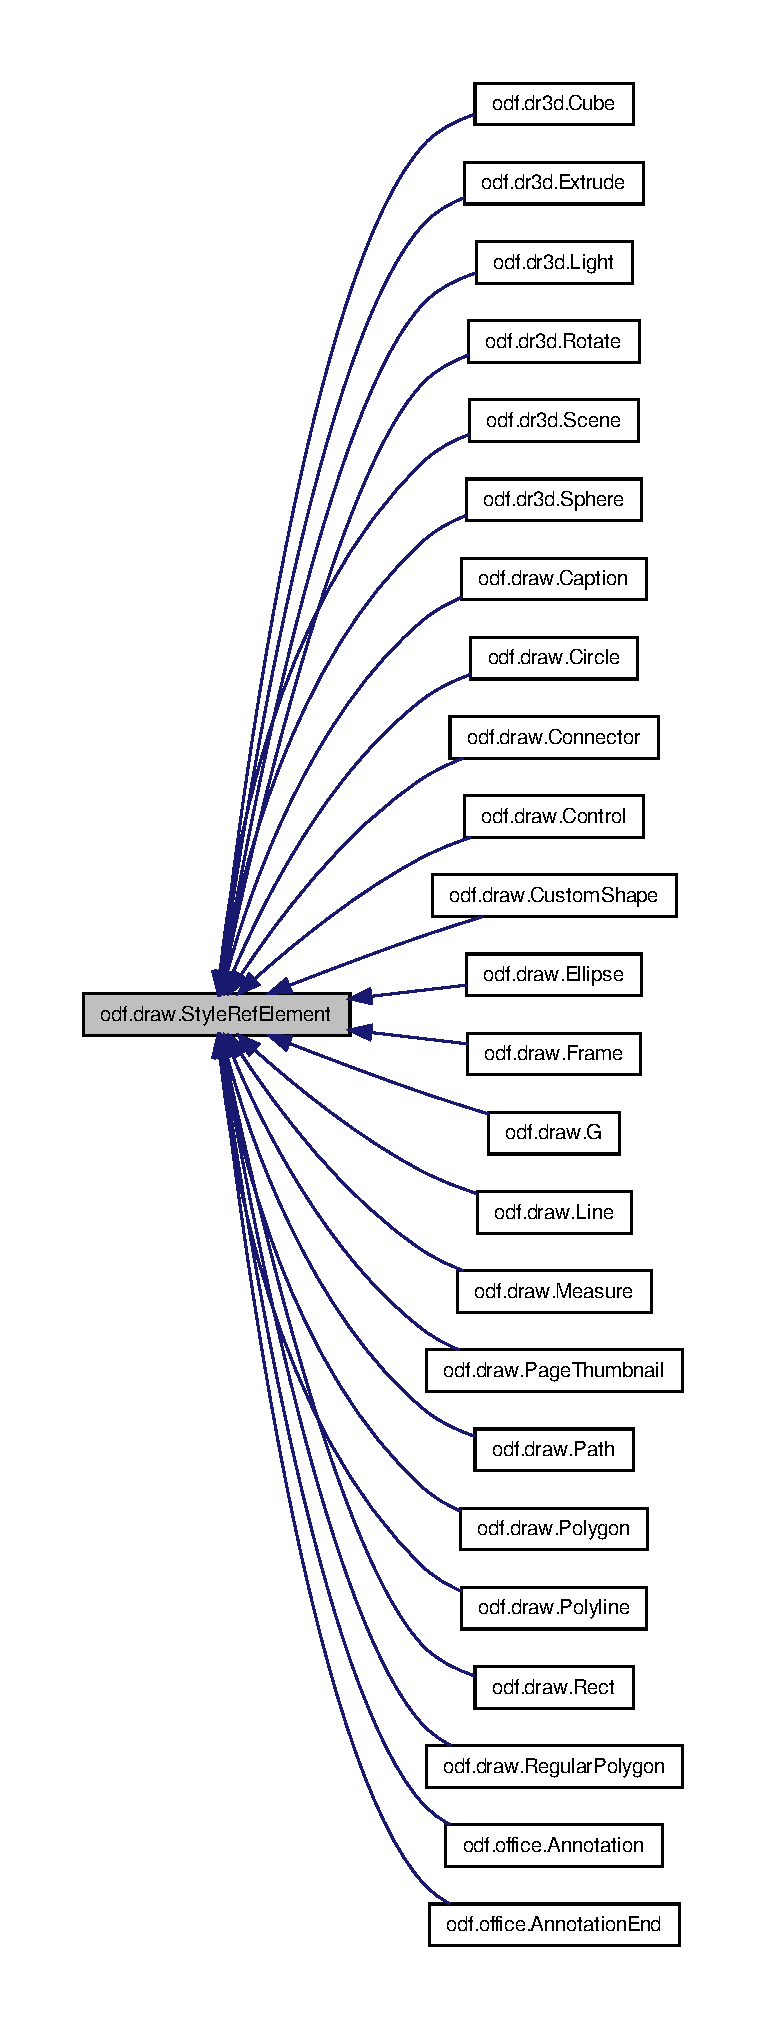
\includegraphics[height=550pt]{namespaceodf_1_1draw_a3370d99ab01e834591bb75a5869210eb_icgraph}
\end{center}
\end{figure}


\hypertarget{namespaceodf_1_1draw_a7cc02a01dccf5779c08f1316aff18eab}{\index{odf\+::draw@{odf\+::draw}!Text\+Box@{Text\+Box}}
\index{Text\+Box@{Text\+Box}!odf\+::draw@{odf\+::draw}}
\subsubsection[{Text\+Box}]{\setlength{\rightskip}{0pt plus 5cm}def odf.\+draw.\+Text\+Box (
\begin{DoxyParamCaption}
\item[{}]{args}
\end{DoxyParamCaption}
)}}\label{namespaceodf_1_1draw_a7cc02a01dccf5779c08f1316aff18eab}


Definition at line 186 of file draw.\+py.


\hypertarget{namespaceodf_1_1easyliststyle}{\section{odf.\+easyliststyle Namespace Reference}
\label{namespaceodf_1_1easyliststyle}\index{odf.\+easyliststyle@{odf.\+easyliststyle}}
}
\subsection*{Functions}
\begin{DoxyCompactItemize}
\item 
def \hyperlink{namespaceodf_1_1easyliststyle_aec199f5afcac7f5d364b79acb2b435ff}{style\+From\+String}
\item 
def \hyperlink{namespaceodf_1_1easyliststyle_ac96c1944732eab4a4cabaf65c05ca411}{style\+From\+List}
\end{DoxyCompactItemize}
\subsection*{Variables}
\begin{DoxyCompactItemize}
\item 
int \hyperlink{namespaceodf_1_1easyliststyle_a3f16b7214e4de8fda12f391a12ca1ae3}{\+\_\+\+M\+A\+X\+\_\+\+L\+I\+S\+T\+\_\+\+L\+E\+V\+E\+L} = 10
\item 
\hyperlink{namespaceodf_1_1easyliststyle_afe20895c55342517506d15451705548a}{S\+H\+O\+W\+\_\+\+A\+L\+L\+\_\+\+L\+E\+V\+E\+L\+S} = True
\item 
\hyperlink{namespaceodf_1_1easyliststyle_aac54725e726263a54b071bae838262b8}{S\+H\+O\+W\+\_\+\+O\+N\+E\+\_\+\+L\+E\+V\+E\+L} = False
\end{DoxyCompactItemize}


\subsection{Function Documentation}
\hypertarget{namespaceodf_1_1easyliststyle_ac96c1944732eab4a4cabaf65c05ca411}{\index{odf\+::easyliststyle@{odf\+::easyliststyle}!style\+From\+List@{style\+From\+List}}
\index{style\+From\+List@{style\+From\+List}!odf\+::easyliststyle@{odf\+::easyliststyle}}
\subsubsection[{style\+From\+List}]{\setlength{\rightskip}{0pt plus 5cm}def odf.\+easyliststyle.\+style\+From\+List (
\begin{DoxyParamCaption}
\item[{}]{style\+Name, }
\item[{}]{spec\+Array, }
\item[{}]{spacing, }
\item[{}]{show\+All\+Levels}
\end{DoxyParamCaption}
)}}\label{namespaceodf_1_1easyliststyle_ac96c1944732eab4a4cabaf65c05ca411}


Definition at line 49 of file easyliststyle.\+py.



Here is the call graph for this function\+:
\nopagebreak
\begin{figure}[H]
\begin{center}
\leavevmode
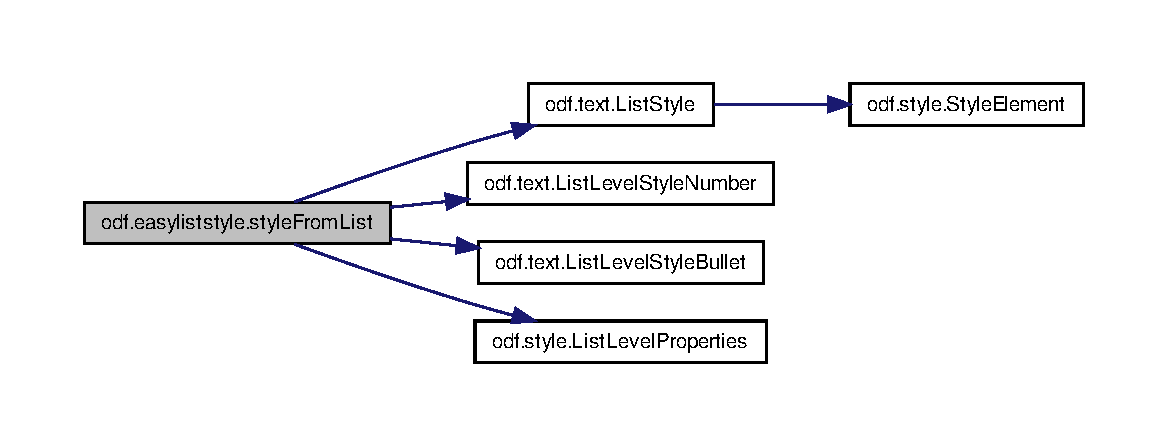
\includegraphics[width=350pt]{namespaceodf_1_1easyliststyle_ac96c1944732eab4a4cabaf65c05ca411_cgraph}
\end{center}
\end{figure}




Here is the caller graph for this function\+:
\nopagebreak
\begin{figure}[H]
\begin{center}
\leavevmode
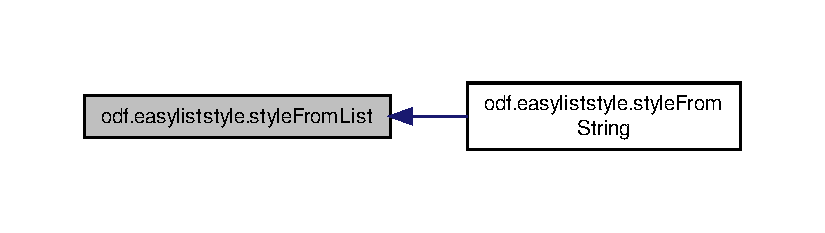
\includegraphics[width=350pt]{namespaceodf_1_1easyliststyle_ac96c1944732eab4a4cabaf65c05ca411_icgraph}
\end{center}
\end{figure}


\hypertarget{namespaceodf_1_1easyliststyle_aec199f5afcac7f5d364b79acb2b435ff}{\index{odf\+::easyliststyle@{odf\+::easyliststyle}!style\+From\+String@{style\+From\+String}}
\index{style\+From\+String@{style\+From\+String}!odf\+::easyliststyle@{odf\+::easyliststyle}}
\subsubsection[{style\+From\+String}]{\setlength{\rightskip}{0pt plus 5cm}def odf.\+easyliststyle.\+style\+From\+String (
\begin{DoxyParamCaption}
\item[{}]{name, }
\item[{}]{specifiers, }
\item[{}]{delim, }
\item[{}]{spacing, }
\item[{}]{show\+All\+Levels}
\end{DoxyParamCaption}
)}}\label{namespaceodf_1_1easyliststyle_aec199f5afcac7f5d364b79acb2b435ff}


Definition at line 45 of file easyliststyle.\+py.



Here is the call graph for this function\+:
\nopagebreak
\begin{figure}[H]
\begin{center}
\leavevmode
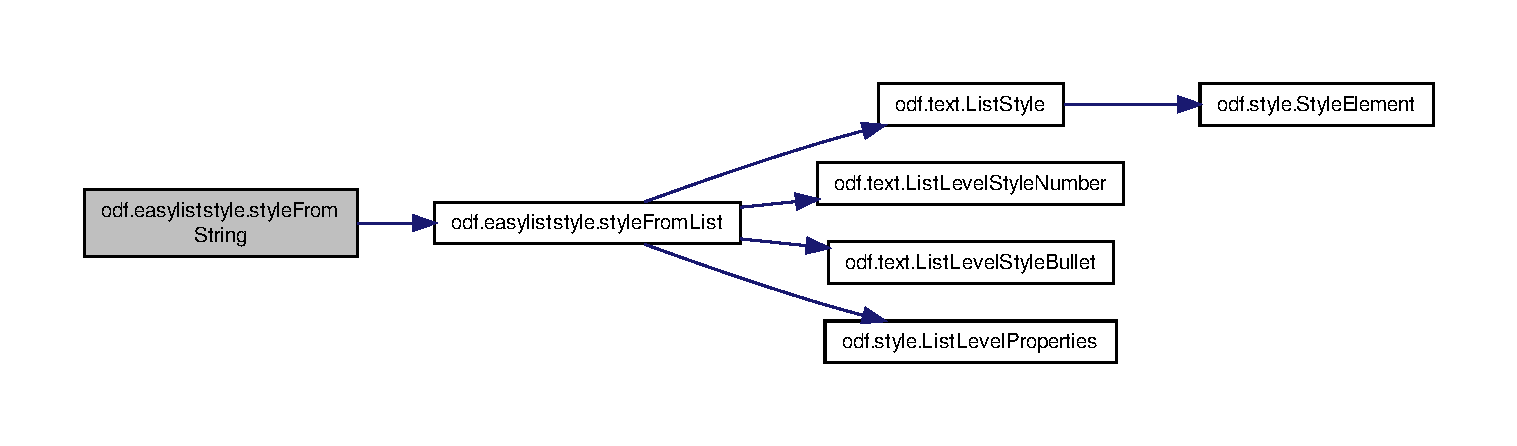
\includegraphics[width=350pt]{namespaceodf_1_1easyliststyle_aec199f5afcac7f5d364b79acb2b435ff_cgraph}
\end{center}
\end{figure}




\subsection{Variable Documentation}
\hypertarget{namespaceodf_1_1easyliststyle_a3f16b7214e4de8fda12f391a12ca1ae3}{\index{odf\+::easyliststyle@{odf\+::easyliststyle}!\+\_\+\+M\+A\+X\+\_\+\+L\+I\+S\+T\+\_\+\+L\+E\+V\+E\+L@{\+\_\+\+M\+A\+X\+\_\+\+L\+I\+S\+T\+\_\+\+L\+E\+V\+E\+L}}
\index{\+\_\+\+M\+A\+X\+\_\+\+L\+I\+S\+T\+\_\+\+L\+E\+V\+E\+L@{\+\_\+\+M\+A\+X\+\_\+\+L\+I\+S\+T\+\_\+\+L\+E\+V\+E\+L}!odf\+::easyliststyle@{odf\+::easyliststyle}}
\subsubsection[{\+\_\+\+M\+A\+X\+\_\+\+L\+I\+S\+T\+\_\+\+L\+E\+V\+E\+L}]{\setlength{\rightskip}{0pt plus 5cm}int odf.\+easyliststyle.\+\_\+\+M\+A\+X\+\_\+\+L\+I\+S\+T\+\_\+\+L\+E\+V\+E\+L = 10}}\label{namespaceodf_1_1easyliststyle_a3f16b7214e4de8fda12f391a12ca1ae3}


Definition at line 41 of file easyliststyle.\+py.

\hypertarget{namespaceodf_1_1easyliststyle_afe20895c55342517506d15451705548a}{\index{odf\+::easyliststyle@{odf\+::easyliststyle}!S\+H\+O\+W\+\_\+\+A\+L\+L\+\_\+\+L\+E\+V\+E\+L\+S@{S\+H\+O\+W\+\_\+\+A\+L\+L\+\_\+\+L\+E\+V\+E\+L\+S}}
\index{S\+H\+O\+W\+\_\+\+A\+L\+L\+\_\+\+L\+E\+V\+E\+L\+S@{S\+H\+O\+W\+\_\+\+A\+L\+L\+\_\+\+L\+E\+V\+E\+L\+S}!odf\+::easyliststyle@{odf\+::easyliststyle}}
\subsubsection[{S\+H\+O\+W\+\_\+\+A\+L\+L\+\_\+\+L\+E\+V\+E\+L\+S}]{\setlength{\rightskip}{0pt plus 5cm}odf.\+easyliststyle.\+S\+H\+O\+W\+\_\+\+A\+L\+L\+\_\+\+L\+E\+V\+E\+L\+S = True}}\label{namespaceodf_1_1easyliststyle_afe20895c55342517506d15451705548a}


Definition at line 42 of file easyliststyle.\+py.

\hypertarget{namespaceodf_1_1easyliststyle_aac54725e726263a54b071bae838262b8}{\index{odf\+::easyliststyle@{odf\+::easyliststyle}!S\+H\+O\+W\+\_\+\+O\+N\+E\+\_\+\+L\+E\+V\+E\+L@{S\+H\+O\+W\+\_\+\+O\+N\+E\+\_\+\+L\+E\+V\+E\+L}}
\index{S\+H\+O\+W\+\_\+\+O\+N\+E\+\_\+\+L\+E\+V\+E\+L@{S\+H\+O\+W\+\_\+\+O\+N\+E\+\_\+\+L\+E\+V\+E\+L}!odf\+::easyliststyle@{odf\+::easyliststyle}}
\subsubsection[{S\+H\+O\+W\+\_\+\+O\+N\+E\+\_\+\+L\+E\+V\+E\+L}]{\setlength{\rightskip}{0pt plus 5cm}odf.\+easyliststyle.\+S\+H\+O\+W\+\_\+\+O\+N\+E\+\_\+\+L\+E\+V\+E\+L = False}}\label{namespaceodf_1_1easyliststyle_aac54725e726263a54b071bae838262b8}


Definition at line 43 of file easyliststyle.\+py.


\hypertarget{namespaceodf_1_1element}{\section{odf.\+element Namespace Reference}
\label{namespaceodf_1_1element}\index{odf.\+element@{odf.\+element}}
}
\subsection*{Classes}
\begin{DoxyCompactItemize}
\item 
class \hyperlink{classodf_1_1element_1_1CDATASection}{C\+D\+A\+T\+A\+Section}
\item 
class \hyperlink{classodf_1_1element_1_1Childless}{Childless}
\begin{DoxyCompactList}\small\item\em Mixin that makes childless-\/ness easy to implement and avoids the complexity of the \hyperlink{classodf_1_1element_1_1Node}{Node} methods that deal with children. \end{DoxyCompactList}\item 
class \hyperlink{classodf_1_1element_1_1Element}{Element}
\begin{DoxyCompactList}\small\item\em Creates a arbitrary element and is intended to be subclassed not used on its own. \end{DoxyCompactList}\item 
class \hyperlink{classodf_1_1element_1_1IllegalChild}{Illegal\+Child}
\begin{DoxyCompactList}\small\item\em Complains if you add an element to a parent where it is not allowed. \end{DoxyCompactList}\item 
class \hyperlink{classodf_1_1element_1_1IllegalText}{Illegal\+Text}
\begin{DoxyCompactList}\small\item\em Complains if you add text or cdata to an element where it is not allowed. \end{DoxyCompactList}\item 
class \hyperlink{classodf_1_1element_1_1Node}{Node}
\begin{DoxyCompactList}\small\item\em super class for more specific nodes \end{DoxyCompactList}\item 
class \hyperlink{classodf_1_1element_1_1Text}{Text}
\end{DoxyCompactItemize}
\subsection*{Variables}
\begin{DoxyCompactItemize}
\item 
\hyperlink{namespaceodf_1_1element_a9474456bb442e238b32a7bdf6a22dcba}{unicode} = str
\end{DoxyCompactItemize}


\subsection{Variable Documentation}
\hypertarget{namespaceodf_1_1element_a9474456bb442e238b32a7bdf6a22dcba}{\index{odf\+::element@{odf\+::element}!unicode@{unicode}}
\index{unicode@{unicode}!odf\+::element@{odf\+::element}}
\subsubsection[{unicode}]{\setlength{\rightskip}{0pt plus 5cm}odf.\+element.\+unicode = str}}\label{namespaceodf_1_1element_a9474456bb442e238b32a7bdf6a22dcba}


Definition at line 34 of file element.\+py.


\hypertarget{namespaceodf_1_1elementtypes}{\section{odf.\+elementtypes Namespace Reference}
\label{namespaceodf_1_1elementtypes}\index{odf.\+elementtypes@{odf.\+elementtypes}}
}
\subsection*{Variables}
\begin{DoxyCompactItemize}
\item 
tuple \hyperlink{namespaceodf_1_1elementtypes_af6af3ee74d3bbcd994b62e093d66efce}{inline\+\_\+elements}
\item 
tuple \hyperlink{namespaceodf_1_1elementtypes_a93bef01e769e000343dd44fd7f0c6857}{block\+\_\+elements}
\item 
tuple \hyperlink{namespaceodf_1_1elementtypes_a0f3fdba85272e773adbe3e184125310f}{declarative\+\_\+elements}
\item 
tuple \hyperlink{namespaceodf_1_1elementtypes_ad5a29e22e6077343a8348bc3d1b13068}{empty\+\_\+elements}
\end{DoxyCompactItemize}


\subsection{Variable Documentation}
\hypertarget{namespaceodf_1_1elementtypes_a93bef01e769e000343dd44fd7f0c6857}{\index{odf\+::elementtypes@{odf\+::elementtypes}!block\+\_\+elements@{block\+\_\+elements}}
\index{block\+\_\+elements@{block\+\_\+elements}!odf\+::elementtypes@{odf\+::elementtypes}}
\subsubsection[{block\+\_\+elements}]{\setlength{\rightskip}{0pt plus 5cm}tuple odf.\+elementtypes.\+block\+\_\+elements}}\label{namespaceodf_1_1elementtypes_a93bef01e769e000343dd44fd7f0c6857}
{\bfseries Initial value\+:}
\begin{DoxyCode}
1 = (
2     (TEXTNS,\textcolor{stringliteral}{u'h'}),
3     (TEXTNS,\textcolor{stringliteral}{u'p'}),
4     (TEXTNS,\textcolor{stringliteral}{u'list'}),
5     (TEXTNS,\textcolor{stringliteral}{u'list-item'}),
6     (TEXTNS,\textcolor{stringliteral}{u'section'}),
7 )
\end{DoxyCode}


Definition at line 114 of file elementtypes.\+py.

\hypertarget{namespaceodf_1_1elementtypes_a0f3fdba85272e773adbe3e184125310f}{\index{odf\+::elementtypes@{odf\+::elementtypes}!declarative\+\_\+elements@{declarative\+\_\+elements}}
\index{declarative\+\_\+elements@{declarative\+\_\+elements}!odf\+::elementtypes@{odf\+::elementtypes}}
\subsubsection[{declarative\+\_\+elements}]{\setlength{\rightskip}{0pt plus 5cm}tuple odf.\+elementtypes.\+declarative\+\_\+elements}}\label{namespaceodf_1_1elementtypes_a0f3fdba85272e773adbe3e184125310f}
{\bfseries Initial value\+:}
\begin{DoxyCode}
1 = (
2     (OFFICENS,\textcolor{stringliteral}{u'font-face-decls'}),
3     (PRESENTATIONNS,\textcolor{stringliteral}{u'date-time-decl'}),
4     (PRESENTATIONNS,\textcolor{stringliteral}{u'footer-decl'}),
5     (PRESENTATIONNS,\textcolor{stringliteral}{u'header-decl'}),
6     (TABLENS,\textcolor{stringliteral}{u'table-template'}),
7     (TEXTNS,\textcolor{stringliteral}{u'alphabetical-index-entry-template'}),
8     (TEXTNS,\textcolor{stringliteral}{u'alphabetical-index-source'}),
9     (TEXTNS,\textcolor{stringliteral}{u'bibliography-entry-template'}),
10     (TEXTNS,\textcolor{stringliteral}{u'bibliography-source'}),
11     (TEXTNS,\textcolor{stringliteral}{u'dde-connection-decls'}),
12     (TEXTNS,\textcolor{stringliteral}{u'illustration-index-entry-template'}),
13     (TEXTNS,\textcolor{stringliteral}{u'illustration-index-source'}),
14     (TEXTNS,\textcolor{stringliteral}{u'index-source-styles'}),
15     (TEXTNS,\textcolor{stringliteral}{u'index-title-template'}),
16     (TEXTNS,\textcolor{stringliteral}{u'note-continuation-notice-backward'}),
17     (TEXTNS,\textcolor{stringliteral}{u'note-continuation-notice-forward'}),
18     (TEXTNS,\textcolor{stringliteral}{u'notes-configuration'}),
19     (TEXTNS,\textcolor{stringliteral}{u'object-index-entry-template'}),
20     (TEXTNS,\textcolor{stringliteral}{u'object-index-source'}),
21     (TEXTNS,\textcolor{stringliteral}{u'sequence-decls'}),
22     (TEXTNS,\textcolor{stringliteral}{u'table-index-entry-template'}),
23     (TEXTNS,\textcolor{stringliteral}{u'table-index-source'}),
24     (TEXTNS,\textcolor{stringliteral}{u'table-of-content-entry-template'}),
25     (TEXTNS,\textcolor{stringliteral}{u'table-of-content-source'}),
26     (TEXTNS,\textcolor{stringliteral}{u'user-field-decls'}),
27     (TEXTNS,\textcolor{stringliteral}{u'user-index-entry-template'}),
28     (TEXTNS,\textcolor{stringliteral}{u'user-index-source'}),
29     (TEXTNS,\textcolor{stringliteral}{u'variable-decls'}),
30 )
\end{DoxyCode}


Definition at line 122 of file elementtypes.\+py.

\hypertarget{namespaceodf_1_1elementtypes_ad5a29e22e6077343a8348bc3d1b13068}{\index{odf\+::elementtypes@{odf\+::elementtypes}!empty\+\_\+elements@{empty\+\_\+elements}}
\index{empty\+\_\+elements@{empty\+\_\+elements}!odf\+::elementtypes@{odf\+::elementtypes}}
\subsubsection[{empty\+\_\+elements}]{\setlength{\rightskip}{0pt plus 5cm}tuple odf.\+elementtypes.\+empty\+\_\+elements}}\label{namespaceodf_1_1elementtypes_ad5a29e22e6077343a8348bc3d1b13068}


Definition at line 153 of file elementtypes.\+py.

\hypertarget{namespaceodf_1_1elementtypes_af6af3ee74d3bbcd994b62e093d66efce}{\index{odf\+::elementtypes@{odf\+::elementtypes}!inline\+\_\+elements@{inline\+\_\+elements}}
\index{inline\+\_\+elements@{inline\+\_\+elements}!odf\+::elementtypes@{odf\+::elementtypes}}
\subsubsection[{inline\+\_\+elements}]{\setlength{\rightskip}{0pt plus 5cm}tuple odf.\+elementtypes.\+inline\+\_\+elements}}\label{namespaceodf_1_1elementtypes_af6af3ee74d3bbcd994b62e093d66efce}


Definition at line 26 of file elementtypes.\+py.


\hypertarget{namespaceodf_1_1form}{\section{odf.\+form Namespace Reference}
\label{namespaceodf_1_1form}\index{odf.\+form@{odf.\+form}}
}
\subsection*{Functions}
\begin{DoxyCompactItemize}
\item 
def \hyperlink{namespaceodf_1_1form_a652dde13416c6041306536a6c0df8bb7}{Button}
\item 
def \hyperlink{namespaceodf_1_1form_a2a2d0201fda6ada48c02ff66de84ed70}{Checkbox}
\item 
def \hyperlink{namespaceodf_1_1form_ada737ba79b60b21fe7150b59aacc90b6}{Column}
\item 
def \hyperlink{namespaceodf_1_1form_a96b747cf3beceb339a7c26bfe9115107}{Combobox}
\item 
def \hyperlink{namespaceodf_1_1form_a86b346c4da24384a61a00bfcc125a8f3}{Connection\+Resource}
\item 
def \hyperlink{namespaceodf_1_1form_aa70310d641c27104cf55cc04963af19a}{Date}
\item 
def \hyperlink{namespaceodf_1_1form_ac9063421d76e60c9f8f4f2f3e2c4da31}{File}
\item 
def \hyperlink{namespaceodf_1_1form_adf2d931853cbd8f4ff6d586499c60faf}{Fixed\+Text}
\item 
def \hyperlink{namespaceodf_1_1form_a91d5b4d72a09e9b115a1cfe441ecacd7}{Form}
\item 
def \hyperlink{namespaceodf_1_1form_a5b88a0820f08ff8b50cd6c2cc8ad9b0c}{Formatted\+Text}
\item 
def \hyperlink{namespaceodf_1_1form_a82a19e3a12817bfaa2f8842387413082}{Frame}
\item 
def \hyperlink{namespaceodf_1_1form_afec8e57920eb45eca1b989d22ebb2f1c}{Generic\+Control}
\item 
def \hyperlink{namespaceodf_1_1form_a4e5cb7e44914b108e06fb9c77b0b2b52}{Grid}
\item 
def \hyperlink{namespaceodf_1_1form_af5561345d3117b0d9f1fb467430a790b}{Hidden}
\item 
def \hyperlink{namespaceodf_1_1form_a96b63942b9bc971dc5c114710544f6b4}{Image}
\item 
def \hyperlink{namespaceodf_1_1form_af87607e975ecda46d82bb5594e135e5c}{Image\+Frame}
\item 
def \hyperlink{namespaceodf_1_1form_a27ff28a057c58093d5298cd9e68bbd5f}{Item}
\item 
def \hyperlink{namespaceodf_1_1form_abe186b40c519081072df07194733685a}{List\+Property}
\item 
def \hyperlink{namespaceodf_1_1form_ac0bdda8ff5b3d11d4eaf40a22f1fd7b4}{List\+Value}
\item 
def \hyperlink{namespaceodf_1_1form_a2baa5f2a1dba03752ca2b1edb2b2509e}{Listbox}
\item 
def \hyperlink{namespaceodf_1_1form_a81e13e985ef81a6d7f2825d18abe20ab}{Number}
\item 
def \hyperlink{namespaceodf_1_1form_a23ebe4053f877da81239e3392dc5da36}{Option}
\item 
def \hyperlink{namespaceodf_1_1form_ae200f1b9f9b67cf87c63b043f042a861}{Password}
\item 
def \hyperlink{namespaceodf_1_1form_a29af724cff187baf9d518028a76e5680}{Properties}
\item 
def \hyperlink{namespaceodf_1_1form_a015a9e29a18ddcdef0a84a5e78e274d9}{Property}
\item 
def \hyperlink{namespaceodf_1_1form_a415e1bfd0b285e10f100126172f883bf}{Radio}
\item 
def \hyperlink{namespaceodf_1_1form_a84ecb785a46d9fc2efa443026f47af76}{Text}
\item 
def \hyperlink{namespaceodf_1_1form_a01daf1fb6eb55f49639527408a75f535}{Textarea}
\item 
def \hyperlink{namespaceodf_1_1form_ae77a558e78aa21c3ec50bce7fe3788d6}{Time}
\item 
def \hyperlink{namespaceodf_1_1form_abe0c191c4044eedf4c32a8dbc5709906}{Value\+Range}
\end{DoxyCompactItemize}


\subsection{Function Documentation}
\hypertarget{namespaceodf_1_1form_a652dde13416c6041306536a6c0df8bb7}{\index{odf\+::form@{odf\+::form}!Button@{Button}}
\index{Button@{Button}!odf\+::form@{odf\+::form}}
\subsubsection[{Button}]{\setlength{\rightskip}{0pt plus 5cm}def odf.\+form.\+Button (
\begin{DoxyParamCaption}
\item[{}]{args}
\end{DoxyParamCaption}
)}}\label{namespaceodf_1_1form_a652dde13416c6041306536a6c0df8bb7}


Definition at line 26 of file form.\+py.

\hypertarget{namespaceodf_1_1form_a2a2d0201fda6ada48c02ff66de84ed70}{\index{odf\+::form@{odf\+::form}!Checkbox@{Checkbox}}
\index{Checkbox@{Checkbox}!odf\+::form@{odf\+::form}}
\subsubsection[{Checkbox}]{\setlength{\rightskip}{0pt plus 5cm}def odf.\+form.\+Checkbox (
\begin{DoxyParamCaption}
\item[{}]{args}
\end{DoxyParamCaption}
)}}\label{namespaceodf_1_1form_a2a2d0201fda6ada48c02ff66de84ed70}


Definition at line 29 of file form.\+py.

\hypertarget{namespaceodf_1_1form_ada737ba79b60b21fe7150b59aacc90b6}{\index{odf\+::form@{odf\+::form}!Column@{Column}}
\index{Column@{Column}!odf\+::form@{odf\+::form}}
\subsubsection[{Column}]{\setlength{\rightskip}{0pt plus 5cm}def odf.\+form.\+Column (
\begin{DoxyParamCaption}
\item[{}]{args}
\end{DoxyParamCaption}
)}}\label{namespaceodf_1_1form_ada737ba79b60b21fe7150b59aacc90b6}


Definition at line 32 of file form.\+py.

\hypertarget{namespaceodf_1_1form_a96b747cf3beceb339a7c26bfe9115107}{\index{odf\+::form@{odf\+::form}!Combobox@{Combobox}}
\index{Combobox@{Combobox}!odf\+::form@{odf\+::form}}
\subsubsection[{Combobox}]{\setlength{\rightskip}{0pt plus 5cm}def odf.\+form.\+Combobox (
\begin{DoxyParamCaption}
\item[{}]{args}
\end{DoxyParamCaption}
)}}\label{namespaceodf_1_1form_a96b747cf3beceb339a7c26bfe9115107}


Definition at line 35 of file form.\+py.

\hypertarget{namespaceodf_1_1form_a86b346c4da24384a61a00bfcc125a8f3}{\index{odf\+::form@{odf\+::form}!Connection\+Resource@{Connection\+Resource}}
\index{Connection\+Resource@{Connection\+Resource}!odf\+::form@{odf\+::form}}
\subsubsection[{Connection\+Resource}]{\setlength{\rightskip}{0pt plus 5cm}def odf.\+form.\+Connection\+Resource (
\begin{DoxyParamCaption}
\item[{}]{args}
\end{DoxyParamCaption}
)}}\label{namespaceodf_1_1form_a86b346c4da24384a61a00bfcc125a8f3}


Definition at line 38 of file form.\+py.

\hypertarget{namespaceodf_1_1form_aa70310d641c27104cf55cc04963af19a}{\index{odf\+::form@{odf\+::form}!Date@{Date}}
\index{Date@{Date}!odf\+::form@{odf\+::form}}
\subsubsection[{Date}]{\setlength{\rightskip}{0pt plus 5cm}def odf.\+form.\+Date (
\begin{DoxyParamCaption}
\item[{}]{args}
\end{DoxyParamCaption}
)}}\label{namespaceodf_1_1form_aa70310d641c27104cf55cc04963af19a}


Definition at line 41 of file form.\+py.

\hypertarget{namespaceodf_1_1form_ac9063421d76e60c9f8f4f2f3e2c4da31}{\index{odf\+::form@{odf\+::form}!File@{File}}
\index{File@{File}!odf\+::form@{odf\+::form}}
\subsubsection[{File}]{\setlength{\rightskip}{0pt plus 5cm}def odf.\+form.\+File (
\begin{DoxyParamCaption}
\item[{}]{args}
\end{DoxyParamCaption}
)}}\label{namespaceodf_1_1form_ac9063421d76e60c9f8f4f2f3e2c4da31}


Definition at line 44 of file form.\+py.

\hypertarget{namespaceodf_1_1form_adf2d931853cbd8f4ff6d586499c60faf}{\index{odf\+::form@{odf\+::form}!Fixed\+Text@{Fixed\+Text}}
\index{Fixed\+Text@{Fixed\+Text}!odf\+::form@{odf\+::form}}
\subsubsection[{Fixed\+Text}]{\setlength{\rightskip}{0pt plus 5cm}def odf.\+form.\+Fixed\+Text (
\begin{DoxyParamCaption}
\item[{}]{args}
\end{DoxyParamCaption}
)}}\label{namespaceodf_1_1form_adf2d931853cbd8f4ff6d586499c60faf}


Definition at line 47 of file form.\+py.

\hypertarget{namespaceodf_1_1form_a91d5b4d72a09e9b115a1cfe441ecacd7}{\index{odf\+::form@{odf\+::form}!Form@{Form}}
\index{Form@{Form}!odf\+::form@{odf\+::form}}
\subsubsection[{Form}]{\setlength{\rightskip}{0pt plus 5cm}def odf.\+form.\+Form (
\begin{DoxyParamCaption}
\item[{}]{args}
\end{DoxyParamCaption}
)}}\label{namespaceodf_1_1form_a91d5b4d72a09e9b115a1cfe441ecacd7}


Definition at line 50 of file form.\+py.

\hypertarget{namespaceodf_1_1form_a5b88a0820f08ff8b50cd6c2cc8ad9b0c}{\index{odf\+::form@{odf\+::form}!Formatted\+Text@{Formatted\+Text}}
\index{Formatted\+Text@{Formatted\+Text}!odf\+::form@{odf\+::form}}
\subsubsection[{Formatted\+Text}]{\setlength{\rightskip}{0pt plus 5cm}def odf.\+form.\+Formatted\+Text (
\begin{DoxyParamCaption}
\item[{}]{args}
\end{DoxyParamCaption}
)}}\label{namespaceodf_1_1form_a5b88a0820f08ff8b50cd6c2cc8ad9b0c}


Definition at line 53 of file form.\+py.

\hypertarget{namespaceodf_1_1form_a82a19e3a12817bfaa2f8842387413082}{\index{odf\+::form@{odf\+::form}!Frame@{Frame}}
\index{Frame@{Frame}!odf\+::form@{odf\+::form}}
\subsubsection[{Frame}]{\setlength{\rightskip}{0pt plus 5cm}def odf.\+form.\+Frame (
\begin{DoxyParamCaption}
\item[{}]{args}
\end{DoxyParamCaption}
)}}\label{namespaceodf_1_1form_a82a19e3a12817bfaa2f8842387413082}


Definition at line 56 of file form.\+py.

\hypertarget{namespaceodf_1_1form_afec8e57920eb45eca1b989d22ebb2f1c}{\index{odf\+::form@{odf\+::form}!Generic\+Control@{Generic\+Control}}
\index{Generic\+Control@{Generic\+Control}!odf\+::form@{odf\+::form}}
\subsubsection[{Generic\+Control}]{\setlength{\rightskip}{0pt plus 5cm}def odf.\+form.\+Generic\+Control (
\begin{DoxyParamCaption}
\item[{}]{args}
\end{DoxyParamCaption}
)}}\label{namespaceodf_1_1form_afec8e57920eb45eca1b989d22ebb2f1c}


Definition at line 59 of file form.\+py.

\hypertarget{namespaceodf_1_1form_a4e5cb7e44914b108e06fb9c77b0b2b52}{\index{odf\+::form@{odf\+::form}!Grid@{Grid}}
\index{Grid@{Grid}!odf\+::form@{odf\+::form}}
\subsubsection[{Grid}]{\setlength{\rightskip}{0pt plus 5cm}def odf.\+form.\+Grid (
\begin{DoxyParamCaption}
\item[{}]{args}
\end{DoxyParamCaption}
)}}\label{namespaceodf_1_1form_a4e5cb7e44914b108e06fb9c77b0b2b52}


Definition at line 62 of file form.\+py.

\hypertarget{namespaceodf_1_1form_af5561345d3117b0d9f1fb467430a790b}{\index{odf\+::form@{odf\+::form}!Hidden@{Hidden}}
\index{Hidden@{Hidden}!odf\+::form@{odf\+::form}}
\subsubsection[{Hidden}]{\setlength{\rightskip}{0pt plus 5cm}def odf.\+form.\+Hidden (
\begin{DoxyParamCaption}
\item[{}]{args}
\end{DoxyParamCaption}
)}}\label{namespaceodf_1_1form_af5561345d3117b0d9f1fb467430a790b}


Definition at line 65 of file form.\+py.

\hypertarget{namespaceodf_1_1form_a96b63942b9bc971dc5c114710544f6b4}{\index{odf\+::form@{odf\+::form}!Image@{Image}}
\index{Image@{Image}!odf\+::form@{odf\+::form}}
\subsubsection[{Image}]{\setlength{\rightskip}{0pt plus 5cm}def odf.\+form.\+Image (
\begin{DoxyParamCaption}
\item[{}]{args}
\end{DoxyParamCaption}
)}}\label{namespaceodf_1_1form_a96b63942b9bc971dc5c114710544f6b4}


Definition at line 68 of file form.\+py.

\hypertarget{namespaceodf_1_1form_af87607e975ecda46d82bb5594e135e5c}{\index{odf\+::form@{odf\+::form}!Image\+Frame@{Image\+Frame}}
\index{Image\+Frame@{Image\+Frame}!odf\+::form@{odf\+::form}}
\subsubsection[{Image\+Frame}]{\setlength{\rightskip}{0pt plus 5cm}def odf.\+form.\+Image\+Frame (
\begin{DoxyParamCaption}
\item[{}]{args}
\end{DoxyParamCaption}
)}}\label{namespaceodf_1_1form_af87607e975ecda46d82bb5594e135e5c}


Definition at line 71 of file form.\+py.

\hypertarget{namespaceodf_1_1form_a27ff28a057c58093d5298cd9e68bbd5f}{\index{odf\+::form@{odf\+::form}!Item@{Item}}
\index{Item@{Item}!odf\+::form@{odf\+::form}}
\subsubsection[{Item}]{\setlength{\rightskip}{0pt plus 5cm}def odf.\+form.\+Item (
\begin{DoxyParamCaption}
\item[{}]{args}
\end{DoxyParamCaption}
)}}\label{namespaceodf_1_1form_a27ff28a057c58093d5298cd9e68bbd5f}


Definition at line 74 of file form.\+py.

\hypertarget{namespaceodf_1_1form_a2baa5f2a1dba03752ca2b1edb2b2509e}{\index{odf\+::form@{odf\+::form}!Listbox@{Listbox}}
\index{Listbox@{Listbox}!odf\+::form@{odf\+::form}}
\subsubsection[{Listbox}]{\setlength{\rightskip}{0pt plus 5cm}def odf.\+form.\+Listbox (
\begin{DoxyParamCaption}
\item[{}]{args}
\end{DoxyParamCaption}
)}}\label{namespaceodf_1_1form_a2baa5f2a1dba03752ca2b1edb2b2509e}


Definition at line 83 of file form.\+py.

\hypertarget{namespaceodf_1_1form_abe186b40c519081072df07194733685a}{\index{odf\+::form@{odf\+::form}!List\+Property@{List\+Property}}
\index{List\+Property@{List\+Property}!odf\+::form@{odf\+::form}}
\subsubsection[{List\+Property}]{\setlength{\rightskip}{0pt plus 5cm}def odf.\+form.\+List\+Property (
\begin{DoxyParamCaption}
\item[{}]{args}
\end{DoxyParamCaption}
)}}\label{namespaceodf_1_1form_abe186b40c519081072df07194733685a}


Definition at line 77 of file form.\+py.

\hypertarget{namespaceodf_1_1form_ac0bdda8ff5b3d11d4eaf40a22f1fd7b4}{\index{odf\+::form@{odf\+::form}!List\+Value@{List\+Value}}
\index{List\+Value@{List\+Value}!odf\+::form@{odf\+::form}}
\subsubsection[{List\+Value}]{\setlength{\rightskip}{0pt plus 5cm}def odf.\+form.\+List\+Value (
\begin{DoxyParamCaption}
\item[{}]{args}
\end{DoxyParamCaption}
)}}\label{namespaceodf_1_1form_ac0bdda8ff5b3d11d4eaf40a22f1fd7b4}


Definition at line 80 of file form.\+py.

\hypertarget{namespaceodf_1_1form_a81e13e985ef81a6d7f2825d18abe20ab}{\index{odf\+::form@{odf\+::form}!Number@{Number}}
\index{Number@{Number}!odf\+::form@{odf\+::form}}
\subsubsection[{Number}]{\setlength{\rightskip}{0pt plus 5cm}def odf.\+form.\+Number (
\begin{DoxyParamCaption}
\item[{}]{args}
\end{DoxyParamCaption}
)}}\label{namespaceodf_1_1form_a81e13e985ef81a6d7f2825d18abe20ab}


Definition at line 86 of file form.\+py.

\hypertarget{namespaceodf_1_1form_a23ebe4053f877da81239e3392dc5da36}{\index{odf\+::form@{odf\+::form}!Option@{Option}}
\index{Option@{Option}!odf\+::form@{odf\+::form}}
\subsubsection[{Option}]{\setlength{\rightskip}{0pt plus 5cm}def odf.\+form.\+Option (
\begin{DoxyParamCaption}
\item[{}]{args}
\end{DoxyParamCaption}
)}}\label{namespaceodf_1_1form_a23ebe4053f877da81239e3392dc5da36}


Definition at line 89 of file form.\+py.

\hypertarget{namespaceodf_1_1form_ae200f1b9f9b67cf87c63b043f042a861}{\index{odf\+::form@{odf\+::form}!Password@{Password}}
\index{Password@{Password}!odf\+::form@{odf\+::form}}
\subsubsection[{Password}]{\setlength{\rightskip}{0pt plus 5cm}def odf.\+form.\+Password (
\begin{DoxyParamCaption}
\item[{}]{args}
\end{DoxyParamCaption}
)}}\label{namespaceodf_1_1form_ae200f1b9f9b67cf87c63b043f042a861}


Definition at line 92 of file form.\+py.

\hypertarget{namespaceodf_1_1form_a29af724cff187baf9d518028a76e5680}{\index{odf\+::form@{odf\+::form}!Properties@{Properties}}
\index{Properties@{Properties}!odf\+::form@{odf\+::form}}
\subsubsection[{Properties}]{\setlength{\rightskip}{0pt plus 5cm}def odf.\+form.\+Properties (
\begin{DoxyParamCaption}
\item[{}]{args}
\end{DoxyParamCaption}
)}}\label{namespaceodf_1_1form_a29af724cff187baf9d518028a76e5680}


Definition at line 95 of file form.\+py.

\hypertarget{namespaceodf_1_1form_a015a9e29a18ddcdef0a84a5e78e274d9}{\index{odf\+::form@{odf\+::form}!Property@{Property}}
\index{Property@{Property}!odf\+::form@{odf\+::form}}
\subsubsection[{Property}]{\setlength{\rightskip}{0pt plus 5cm}def odf.\+form.\+Property (
\begin{DoxyParamCaption}
\item[{}]{args}
\end{DoxyParamCaption}
)}}\label{namespaceodf_1_1form_a015a9e29a18ddcdef0a84a5e78e274d9}


Definition at line 98 of file form.\+py.

\hypertarget{namespaceodf_1_1form_a415e1bfd0b285e10f100126172f883bf}{\index{odf\+::form@{odf\+::form}!Radio@{Radio}}
\index{Radio@{Radio}!odf\+::form@{odf\+::form}}
\subsubsection[{Radio}]{\setlength{\rightskip}{0pt plus 5cm}def odf.\+form.\+Radio (
\begin{DoxyParamCaption}
\item[{}]{args}
\end{DoxyParamCaption}
)}}\label{namespaceodf_1_1form_a415e1bfd0b285e10f100126172f883bf}


Definition at line 101 of file form.\+py.

\hypertarget{namespaceodf_1_1form_a84ecb785a46d9fc2efa443026f47af76}{\index{odf\+::form@{odf\+::form}!Text@{Text}}
\index{Text@{Text}!odf\+::form@{odf\+::form}}
\subsubsection[{Text}]{\setlength{\rightskip}{0pt plus 5cm}def odf.\+form.\+Text (
\begin{DoxyParamCaption}
\item[{}]{args}
\end{DoxyParamCaption}
)}}\label{namespaceodf_1_1form_a84ecb785a46d9fc2efa443026f47af76}


Definition at line 104 of file form.\+py.



Here is the caller graph for this function\+:
\nopagebreak
\begin{figure}[H]
\begin{center}
\leavevmode
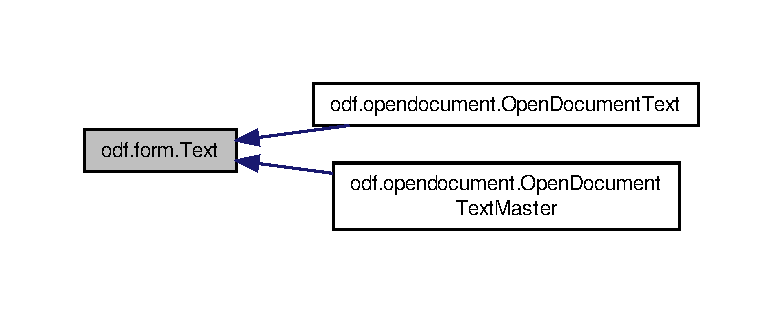
\includegraphics[width=350pt]{namespaceodf_1_1form_a84ecb785a46d9fc2efa443026f47af76_icgraph}
\end{center}
\end{figure}


\hypertarget{namespaceodf_1_1form_a01daf1fb6eb55f49639527408a75f535}{\index{odf\+::form@{odf\+::form}!Textarea@{Textarea}}
\index{Textarea@{Textarea}!odf\+::form@{odf\+::form}}
\subsubsection[{Textarea}]{\setlength{\rightskip}{0pt plus 5cm}def odf.\+form.\+Textarea (
\begin{DoxyParamCaption}
\item[{}]{args}
\end{DoxyParamCaption}
)}}\label{namespaceodf_1_1form_a01daf1fb6eb55f49639527408a75f535}


Definition at line 107 of file form.\+py.

\hypertarget{namespaceodf_1_1form_ae77a558e78aa21c3ec50bce7fe3788d6}{\index{odf\+::form@{odf\+::form}!Time@{Time}}
\index{Time@{Time}!odf\+::form@{odf\+::form}}
\subsubsection[{Time}]{\setlength{\rightskip}{0pt plus 5cm}def odf.\+form.\+Time (
\begin{DoxyParamCaption}
\item[{}]{args}
\end{DoxyParamCaption}
)}}\label{namespaceodf_1_1form_ae77a558e78aa21c3ec50bce7fe3788d6}


Definition at line 110 of file form.\+py.

\hypertarget{namespaceodf_1_1form_abe0c191c4044eedf4c32a8dbc5709906}{\index{odf\+::form@{odf\+::form}!Value\+Range@{Value\+Range}}
\index{Value\+Range@{Value\+Range}!odf\+::form@{odf\+::form}}
\subsubsection[{Value\+Range}]{\setlength{\rightskip}{0pt plus 5cm}def odf.\+form.\+Value\+Range (
\begin{DoxyParamCaption}
\item[{}]{args}
\end{DoxyParamCaption}
)}}\label{namespaceodf_1_1form_abe0c191c4044eedf4c32a8dbc5709906}


Definition at line 113 of file form.\+py.


\hypertarget{namespaceodf_1_1grammar}{\section{odf.\+grammar Namespace Reference}
\label{namespaceodf_1_1grammar}\index{odf.\+grammar@{odf.\+grammar}}
}
\subsection*{Variables}
\begin{DoxyCompactItemize}
\item 
string \hyperlink{namespaceodf_1_1grammar_acef64e7e05d460461ee25112dae95882}{\+\_\+\+\_\+doc\+\_\+\+\_\+}
\item 
dictionary \hyperlink{namespaceodf_1_1grammar_afedffb9bc285b6d478b821ee6f27db49}{allowed\+\_\+children}
\item 
tuple \hyperlink{namespaceodf_1_1grammar_af74bda0d0f630e9047b1d30972fb8892}{allows\+\_\+text}
\item 
dictionary \hyperlink{namespaceodf_1_1grammar_a5a5da9502e3a9a572fe272da463f1877}{required\+\_\+attributes}
\item 
dictionary \hyperlink{namespaceodf_1_1grammar_a977fc09293e3ad44040d3d0dd5d76e50}{allowed\+\_\+attributes}
\end{DoxyCompactItemize}


\subsection{Variable Documentation}
\hypertarget{namespaceodf_1_1grammar_acef64e7e05d460461ee25112dae95882}{\index{odf\+::grammar@{odf\+::grammar}!\+\_\+\+\_\+doc\+\_\+\+\_\+@{\+\_\+\+\_\+doc\+\_\+\+\_\+}}
\index{\+\_\+\+\_\+doc\+\_\+\+\_\+@{\+\_\+\+\_\+doc\+\_\+\+\_\+}!odf\+::grammar@{odf\+::grammar}}
\subsubsection[{\+\_\+\+\_\+doc\+\_\+\+\_\+}]{\setlength{\rightskip}{0pt plus 5cm}string odf.\+grammar.\+\_\+\+\_\+doc\+\_\+\+\_\+}}\label{namespaceodf_1_1grammar_acef64e7e05d460461ee25112dae95882}
{\bfseries Initial value\+:}
\begin{DoxyCode}
1 = \textcolor{stringliteral}{""" In principle the OpenDocument schema converted to python structures.}
2 \textcolor{stringliteral}{Currently it contains the legal child elements of a given element.}
3 \textcolor{stringliteral}{To be used for validation check in the API}
4 \textcolor{stringliteral}{"""}
\end{DoxyCode}


Definition at line 21 of file grammar.\+py.

\hypertarget{namespaceodf_1_1grammar_a977fc09293e3ad44040d3d0dd5d76e50}{\index{odf\+::grammar@{odf\+::grammar}!allowed\+\_\+attributes@{allowed\+\_\+attributes}}
\index{allowed\+\_\+attributes@{allowed\+\_\+attributes}!odf\+::grammar@{odf\+::grammar}}
\subsubsection[{allowed\+\_\+attributes}]{\setlength{\rightskip}{0pt plus 5cm}dictionary odf.\+grammar.\+allowed\+\_\+attributes}}\label{namespaceodf_1_1grammar_a977fc09293e3ad44040d3d0dd5d76e50}


Definition at line 4678 of file grammar.\+py.

\hypertarget{namespaceodf_1_1grammar_afedffb9bc285b6d478b821ee6f27db49}{\index{odf\+::grammar@{odf\+::grammar}!allowed\+\_\+children@{allowed\+\_\+children}}
\index{allowed\+\_\+children@{allowed\+\_\+children}!odf\+::grammar@{odf\+::grammar}}
\subsubsection[{allowed\+\_\+children}]{\setlength{\rightskip}{0pt plus 5cm}dictionary odf.\+grammar.\+allowed\+\_\+children}}\label{namespaceodf_1_1grammar_afedffb9bc285b6d478b821ee6f27db49}


Definition at line 62 of file grammar.\+py.

\hypertarget{namespaceodf_1_1grammar_af74bda0d0f630e9047b1d30972fb8892}{\index{odf\+::grammar@{odf\+::grammar}!allows\+\_\+text@{allows\+\_\+text}}
\index{allows\+\_\+text@{allows\+\_\+text}!odf\+::grammar@{odf\+::grammar}}
\subsubsection[{allows\+\_\+text}]{\setlength{\rightskip}{0pt plus 5cm}tuple odf.\+grammar.\+allows\+\_\+text}}\label{namespaceodf_1_1grammar_af74bda0d0f630e9047b1d30972fb8892}


Definition at line 3619 of file grammar.\+py.

\hypertarget{namespaceodf_1_1grammar_a5a5da9502e3a9a572fe272da463f1877}{\index{odf\+::grammar@{odf\+::grammar}!required\+\_\+attributes@{required\+\_\+attributes}}
\index{required\+\_\+attributes@{required\+\_\+attributes}!odf\+::grammar@{odf\+::grammar}}
\subsubsection[{required\+\_\+attributes}]{\setlength{\rightskip}{0pt plus 5cm}dictionary odf.\+grammar.\+required\+\_\+attributes}}\label{namespaceodf_1_1grammar_a5a5da9502e3a9a572fe272da463f1877}


Definition at line 3761 of file grammar.\+py.


\hypertarget{namespaceodf_1_1load}{\section{odf.\+load Namespace Reference}
\label{namespaceodf_1_1load}\index{odf.\+load@{odf.\+load}}
}
\subsection*{Classes}
\begin{DoxyCompactItemize}
\item 
class \hyperlink{classodf_1_1load_1_1LoadParser}{Load\+Parser}
\begin{DoxyCompactList}\small\item\em Extract headings from content.\+xml of an O\+D\+T file. \end{DoxyCompactList}\end{DoxyCompactItemize}

\hypertarget{namespaceodf_1_1manifest}{\section{odf.\+manifest Namespace Reference}
\label{namespaceodf_1_1manifest}\index{odf.\+manifest@{odf.\+manifest}}
}
\subsection*{Functions}
\begin{DoxyCompactItemize}
\item 
def \hyperlink{namespaceodf_1_1manifest_a50638c6f7e5ca13cfad81308c02e805d}{Manifest}
\item 
def \hyperlink{namespaceodf_1_1manifest_a2628bc06ca72edff6263a23448bbd884}{File\+Entry}
\item 
def \hyperlink{namespaceodf_1_1manifest_a8b27a956d61e42b1d9595810ec7cba99}{Encryption\+Data}
\item 
def \hyperlink{namespaceodf_1_1manifest_a7ea1152fd7bd64a3e37af2549c6fe88a}{Algorithm}
\item 
def \hyperlink{namespaceodf_1_1manifest_a91334592da1a5428af9045883869ebe8}{Key\+Derivation}
\end{DoxyCompactItemize}


\subsection{Function Documentation}
\hypertarget{namespaceodf_1_1manifest_a7ea1152fd7bd64a3e37af2549c6fe88a}{\index{odf\+::manifest@{odf\+::manifest}!Algorithm@{Algorithm}}
\index{Algorithm@{Algorithm}!odf\+::manifest@{odf\+::manifest}}
\subsubsection[{Algorithm}]{\setlength{\rightskip}{0pt plus 5cm}def odf.\+manifest.\+Algorithm (
\begin{DoxyParamCaption}
\item[{}]{args}
\end{DoxyParamCaption}
)}}\label{namespaceodf_1_1manifest_a7ea1152fd7bd64a3e37af2549c6fe88a}


Definition at line 39 of file manifest.\+py.

\hypertarget{namespaceodf_1_1manifest_a8b27a956d61e42b1d9595810ec7cba99}{\index{odf\+::manifest@{odf\+::manifest}!Encryption\+Data@{Encryption\+Data}}
\index{Encryption\+Data@{Encryption\+Data}!odf\+::manifest@{odf\+::manifest}}
\subsubsection[{Encryption\+Data}]{\setlength{\rightskip}{0pt plus 5cm}def odf.\+manifest.\+Encryption\+Data (
\begin{DoxyParamCaption}
\item[{}]{args}
\end{DoxyParamCaption}
)}}\label{namespaceodf_1_1manifest_a8b27a956d61e42b1d9595810ec7cba99}


Definition at line 36 of file manifest.\+py.

\hypertarget{namespaceodf_1_1manifest_a2628bc06ca72edff6263a23448bbd884}{\index{odf\+::manifest@{odf\+::manifest}!File\+Entry@{File\+Entry}}
\index{File\+Entry@{File\+Entry}!odf\+::manifest@{odf\+::manifest}}
\subsubsection[{File\+Entry}]{\setlength{\rightskip}{0pt plus 5cm}def odf.\+manifest.\+File\+Entry (
\begin{DoxyParamCaption}
\item[{}]{args}
\end{DoxyParamCaption}
)}}\label{namespaceodf_1_1manifest_a2628bc06ca72edff6263a23448bbd884}


Definition at line 33 of file manifest.\+py.

\hypertarget{namespaceodf_1_1manifest_a91334592da1a5428af9045883869ebe8}{\index{odf\+::manifest@{odf\+::manifest}!Key\+Derivation@{Key\+Derivation}}
\index{Key\+Derivation@{Key\+Derivation}!odf\+::manifest@{odf\+::manifest}}
\subsubsection[{Key\+Derivation}]{\setlength{\rightskip}{0pt plus 5cm}def odf.\+manifest.\+Key\+Derivation (
\begin{DoxyParamCaption}
\item[{}]{args}
\end{DoxyParamCaption}
)}}\label{namespaceodf_1_1manifest_a91334592da1a5428af9045883869ebe8}


Definition at line 42 of file manifest.\+py.

\hypertarget{namespaceodf_1_1manifest_a50638c6f7e5ca13cfad81308c02e805d}{\index{odf\+::manifest@{odf\+::manifest}!Manifest@{Manifest}}
\index{Manifest@{Manifest}!odf\+::manifest@{odf\+::manifest}}
\subsubsection[{Manifest}]{\setlength{\rightskip}{0pt plus 5cm}def odf.\+manifest.\+Manifest (
\begin{DoxyParamCaption}
\item[{}]{args}
\end{DoxyParamCaption}
)}}\label{namespaceodf_1_1manifest_a50638c6f7e5ca13cfad81308c02e805d}


Definition at line 30 of file manifest.\+py.


\hypertarget{namespaceodf_1_1math}{\section{odf.\+math Namespace Reference}
\label{namespaceodf_1_1math}\index{odf.\+math@{odf.\+math}}
}
\subsection*{Functions}
\begin{DoxyCompactItemize}
\item 
def \hyperlink{namespaceodf_1_1math_ad2e100e4694f7fce0a3db20907e094c2}{Math}
\end{DoxyCompactItemize}


\subsection{Function Documentation}
\hypertarget{namespaceodf_1_1math_ad2e100e4694f7fce0a3db20907e094c2}{\index{odf\+::math@{odf\+::math}!Math@{Math}}
\index{Math@{Math}!odf\+::math@{odf\+::math}}
\subsubsection[{Math}]{\setlength{\rightskip}{0pt plus 5cm}def odf.\+math.\+Math (
\begin{DoxyParamCaption}
\item[{}]{args}
\end{DoxyParamCaption}
)}}\label{namespaceodf_1_1math_ad2e100e4694f7fce0a3db20907e094c2}


Definition at line 28 of file math.\+py.


\hypertarget{namespaceodf_1_1meta}{\section{odf.\+meta Namespace Reference}
\label{namespaceodf_1_1meta}\index{odf.\+meta@{odf.\+meta}}
}
\subsection*{Functions}
\begin{DoxyCompactItemize}
\item 
def \hyperlink{namespaceodf_1_1meta_a56f8e703d81c98e516a4964b2381b869}{Auto\+Reload}
\item 
def \hyperlink{namespaceodf_1_1meta_a8030344c0edaa27ab1176185dd0144b2}{Creation\+Date}
\item 
def \hyperlink{namespaceodf_1_1meta_a567835aab7fba93aa9ce9f659fe20e12}{Date\+String}
\item 
def \hyperlink{namespaceodf_1_1meta_a3e9b0f205c9211c3c31452aeca178a08}{Document\+Statistic}
\item 
def \hyperlink{namespaceodf_1_1meta_a782529060de4047c0337ad45a927af74}{Editing\+Cycles}
\item 
def \hyperlink{namespaceodf_1_1meta_aef8041b653eb35c475a9d5a00d685dab}{Editing\+Duration}
\item 
def \hyperlink{namespaceodf_1_1meta_af358679847dc4f8640f812b78207eac5}{Generator}
\item 
def \hyperlink{namespaceodf_1_1meta_ae013d09a62e1a8a664262af49719bc53}{Hyperlink\+Behaviour}
\item 
def \hyperlink{namespaceodf_1_1meta_a734ee7748a850249d7aa80f8b240bfd6}{Initial\+Creator}
\item 
def \hyperlink{namespaceodf_1_1meta_a49e6c8de501570010e6361810100ae31}{Keyword}
\item 
def \hyperlink{namespaceodf_1_1meta_a47ca1c2ae0f21de9edb7936f2d637924}{Print\+Date}
\item 
def \hyperlink{namespaceodf_1_1meta_a1c2b90d3c21ff51af4db4221f53aff70}{Printed\+By}
\item 
def \hyperlink{namespaceodf_1_1meta_a2315ca939af7c164b441e1ef3def6530}{Template}
\item 
def \hyperlink{namespaceodf_1_1meta_a54f5d4628158f4535d6d80212213b6df}{User\+Defined}
\end{DoxyCompactItemize}


\subsection{Function Documentation}
\hypertarget{namespaceodf_1_1meta_a56f8e703d81c98e516a4964b2381b869}{\index{odf\+::meta@{odf\+::meta}!Auto\+Reload@{Auto\+Reload}}
\index{Auto\+Reload@{Auto\+Reload}!odf\+::meta@{odf\+::meta}}
\subsubsection[{Auto\+Reload}]{\setlength{\rightskip}{0pt plus 5cm}def odf.\+meta.\+Auto\+Reload (
\begin{DoxyParamCaption}
\item[{}]{args}
\end{DoxyParamCaption}
)}}\label{namespaceodf_1_1meta_a56f8e703d81c98e516a4964b2381b869}


Definition at line 25 of file meta.\+py.

\hypertarget{namespaceodf_1_1meta_a8030344c0edaa27ab1176185dd0144b2}{\index{odf\+::meta@{odf\+::meta}!Creation\+Date@{Creation\+Date}}
\index{Creation\+Date@{Creation\+Date}!odf\+::meta@{odf\+::meta}}
\subsubsection[{Creation\+Date}]{\setlength{\rightskip}{0pt plus 5cm}def odf.\+meta.\+Creation\+Date (
\begin{DoxyParamCaption}
\item[{}]{args}
\end{DoxyParamCaption}
)}}\label{namespaceodf_1_1meta_a8030344c0edaa27ab1176185dd0144b2}


Definition at line 28 of file meta.\+py.

\hypertarget{namespaceodf_1_1meta_a567835aab7fba93aa9ce9f659fe20e12}{\index{odf\+::meta@{odf\+::meta}!Date\+String@{Date\+String}}
\index{Date\+String@{Date\+String}!odf\+::meta@{odf\+::meta}}
\subsubsection[{Date\+String}]{\setlength{\rightskip}{0pt plus 5cm}def odf.\+meta.\+Date\+String (
\begin{DoxyParamCaption}
\item[{}]{args}
\end{DoxyParamCaption}
)}}\label{namespaceodf_1_1meta_a567835aab7fba93aa9ce9f659fe20e12}


Definition at line 31 of file meta.\+py.

\hypertarget{namespaceodf_1_1meta_a3e9b0f205c9211c3c31452aeca178a08}{\index{odf\+::meta@{odf\+::meta}!Document\+Statistic@{Document\+Statistic}}
\index{Document\+Statistic@{Document\+Statistic}!odf\+::meta@{odf\+::meta}}
\subsubsection[{Document\+Statistic}]{\setlength{\rightskip}{0pt plus 5cm}def odf.\+meta.\+Document\+Statistic (
\begin{DoxyParamCaption}
\item[{}]{args}
\end{DoxyParamCaption}
)}}\label{namespaceodf_1_1meta_a3e9b0f205c9211c3c31452aeca178a08}


Definition at line 34 of file meta.\+py.

\hypertarget{namespaceodf_1_1meta_a782529060de4047c0337ad45a927af74}{\index{odf\+::meta@{odf\+::meta}!Editing\+Cycles@{Editing\+Cycles}}
\index{Editing\+Cycles@{Editing\+Cycles}!odf\+::meta@{odf\+::meta}}
\subsubsection[{Editing\+Cycles}]{\setlength{\rightskip}{0pt plus 5cm}def odf.\+meta.\+Editing\+Cycles (
\begin{DoxyParamCaption}
\item[{}]{args}
\end{DoxyParamCaption}
)}}\label{namespaceodf_1_1meta_a782529060de4047c0337ad45a927af74}


Definition at line 37 of file meta.\+py.

\hypertarget{namespaceodf_1_1meta_aef8041b653eb35c475a9d5a00d685dab}{\index{odf\+::meta@{odf\+::meta}!Editing\+Duration@{Editing\+Duration}}
\index{Editing\+Duration@{Editing\+Duration}!odf\+::meta@{odf\+::meta}}
\subsubsection[{Editing\+Duration}]{\setlength{\rightskip}{0pt plus 5cm}def odf.\+meta.\+Editing\+Duration (
\begin{DoxyParamCaption}
\item[{}]{args}
\end{DoxyParamCaption}
)}}\label{namespaceodf_1_1meta_aef8041b653eb35c475a9d5a00d685dab}


Definition at line 40 of file meta.\+py.

\hypertarget{namespaceodf_1_1meta_af358679847dc4f8640f812b78207eac5}{\index{odf\+::meta@{odf\+::meta}!Generator@{Generator}}
\index{Generator@{Generator}!odf\+::meta@{odf\+::meta}}
\subsubsection[{Generator}]{\setlength{\rightskip}{0pt plus 5cm}def odf.\+meta.\+Generator (
\begin{DoxyParamCaption}
\item[{}]{args}
\end{DoxyParamCaption}
)}}\label{namespaceodf_1_1meta_af358679847dc4f8640f812b78207eac5}


Definition at line 43 of file meta.\+py.

\hypertarget{namespaceodf_1_1meta_ae013d09a62e1a8a664262af49719bc53}{\index{odf\+::meta@{odf\+::meta}!Hyperlink\+Behaviour@{Hyperlink\+Behaviour}}
\index{Hyperlink\+Behaviour@{Hyperlink\+Behaviour}!odf\+::meta@{odf\+::meta}}
\subsubsection[{Hyperlink\+Behaviour}]{\setlength{\rightskip}{0pt plus 5cm}def odf.\+meta.\+Hyperlink\+Behaviour (
\begin{DoxyParamCaption}
\item[{}]{args}
\end{DoxyParamCaption}
)}}\label{namespaceodf_1_1meta_ae013d09a62e1a8a664262af49719bc53}


Definition at line 46 of file meta.\+py.

\hypertarget{namespaceodf_1_1meta_a734ee7748a850249d7aa80f8b240bfd6}{\index{odf\+::meta@{odf\+::meta}!Initial\+Creator@{Initial\+Creator}}
\index{Initial\+Creator@{Initial\+Creator}!odf\+::meta@{odf\+::meta}}
\subsubsection[{Initial\+Creator}]{\setlength{\rightskip}{0pt plus 5cm}def odf.\+meta.\+Initial\+Creator (
\begin{DoxyParamCaption}
\item[{}]{args}
\end{DoxyParamCaption}
)}}\label{namespaceodf_1_1meta_a734ee7748a850249d7aa80f8b240bfd6}


Definition at line 49 of file meta.\+py.

\hypertarget{namespaceodf_1_1meta_a49e6c8de501570010e6361810100ae31}{\index{odf\+::meta@{odf\+::meta}!Keyword@{Keyword}}
\index{Keyword@{Keyword}!odf\+::meta@{odf\+::meta}}
\subsubsection[{Keyword}]{\setlength{\rightskip}{0pt plus 5cm}def odf.\+meta.\+Keyword (
\begin{DoxyParamCaption}
\item[{}]{args}
\end{DoxyParamCaption}
)}}\label{namespaceodf_1_1meta_a49e6c8de501570010e6361810100ae31}


Definition at line 52 of file meta.\+py.

\hypertarget{namespaceodf_1_1meta_a47ca1c2ae0f21de9edb7936f2d637924}{\index{odf\+::meta@{odf\+::meta}!Print\+Date@{Print\+Date}}
\index{Print\+Date@{Print\+Date}!odf\+::meta@{odf\+::meta}}
\subsubsection[{Print\+Date}]{\setlength{\rightskip}{0pt plus 5cm}def odf.\+meta.\+Print\+Date (
\begin{DoxyParamCaption}
\item[{}]{args}
\end{DoxyParamCaption}
)}}\label{namespaceodf_1_1meta_a47ca1c2ae0f21de9edb7936f2d637924}


Definition at line 55 of file meta.\+py.

\hypertarget{namespaceodf_1_1meta_a1c2b90d3c21ff51af4db4221f53aff70}{\index{odf\+::meta@{odf\+::meta}!Printed\+By@{Printed\+By}}
\index{Printed\+By@{Printed\+By}!odf\+::meta@{odf\+::meta}}
\subsubsection[{Printed\+By}]{\setlength{\rightskip}{0pt plus 5cm}def odf.\+meta.\+Printed\+By (
\begin{DoxyParamCaption}
\item[{}]{args}
\end{DoxyParamCaption}
)}}\label{namespaceodf_1_1meta_a1c2b90d3c21ff51af4db4221f53aff70}


Definition at line 58 of file meta.\+py.

\hypertarget{namespaceodf_1_1meta_a2315ca939af7c164b441e1ef3def6530}{\index{odf\+::meta@{odf\+::meta}!Template@{Template}}
\index{Template@{Template}!odf\+::meta@{odf\+::meta}}
\subsubsection[{Template}]{\setlength{\rightskip}{0pt plus 5cm}def odf.\+meta.\+Template (
\begin{DoxyParamCaption}
\item[{}]{args}
\end{DoxyParamCaption}
)}}\label{namespaceodf_1_1meta_a2315ca939af7c164b441e1ef3def6530}


Definition at line 61 of file meta.\+py.

\hypertarget{namespaceodf_1_1meta_a54f5d4628158f4535d6d80212213b6df}{\index{odf\+::meta@{odf\+::meta}!User\+Defined@{User\+Defined}}
\index{User\+Defined@{User\+Defined}!odf\+::meta@{odf\+::meta}}
\subsubsection[{User\+Defined}]{\setlength{\rightskip}{0pt plus 5cm}def odf.\+meta.\+User\+Defined (
\begin{DoxyParamCaption}
\item[{}]{args}
\end{DoxyParamCaption}
)}}\label{namespaceodf_1_1meta_a54f5d4628158f4535d6d80212213b6df}


Definition at line 65 of file meta.\+py.


\hypertarget{namespaceodf_1_1namespaces}{\section{odf.\+namespaces Namespace Reference}
\label{namespaceodf_1_1namespaces}\index{odf.\+namespaces@{odf.\+namespaces}}
}
\subsection*{Variables}
\begin{DoxyCompactItemize}
\item 
string \hyperlink{namespaceodf_1_1namespaces_a736381c711ff84b4eb1438250d37c47c}{T\+O\+O\+L\+S\+V\+E\+R\+S\+I\+O\+N} = u\char`\"{}O\+D\+F\+P\+Y/1.\+2.\+0dev\char`\"{}
\item 
string \hyperlink{namespaceodf_1_1namespaces_a799446ad85a3db054a63ef0c7eb613a6}{A\+N\+I\+M\+N\+S} = u\char`\"{}urn\+:oasis\+:names\+:tc\+:opendocument\+:xmlns\+:animation\+:1.\+0\char`\"{}
\item 
string \hyperlink{namespaceodf_1_1namespaces_abcad86ac6d4ff8db343d42fe9d81cf69}{C\+H\+A\+R\+T\+N\+S} = u\char`\"{}urn\+:oasis\+:names\+:tc\+:opendocument\+:xmlns\+:chart\+:1.\+0\char`\"{}
\item 
string \hyperlink{namespaceodf_1_1namespaces_a94cf86979bbde22bd25d4a867f6329df}{C\+H\+A\+R\+T\+O\+O\+O\+N\+S} = u\char`\"{}http\+://openoffice.\+org/2010/chart\char`\"{}
\item 
string \hyperlink{namespaceodf_1_1namespaces_aa10cc99f2e65577ec7fa203cf7c7be34}{C\+O\+N\+F\+I\+G\+N\+S} = u\char`\"{}urn\+:oasis\+:names\+:tc\+:opendocument\+:xmlns\+:config\+:1.\+0\char`\"{}
\item 
string \hyperlink{namespaceodf_1_1namespaces_a72fa2c70a996fefada2f9b239b2a3847}{C\+S\+S3\+T\+N\+S} = u\char`\"{}http\+://www.\+w3.\+org/T\+R/css3-\/text/\char`\"{}
\item 
string \hyperlink{namespaceodf_1_1namespaces_a8af54ab4f35bb100600ecebb18bef049}{D\+B\+N\+S} = u\char`\"{}urn\+:oasis\+:names\+:tc\+:opendocument\+:xmlns\+:database\+:1.\+0\char`\"{}
\item 
string \hyperlink{namespaceodf_1_1namespaces_abc0ff10411221c32712c3027f62f8d21}{D\+C\+N\+S} = u\char`\"{}http\+://purl.\+org/dc/elements/1.\+1/\char`\"{}
\item 
string \hyperlink{namespaceodf_1_1namespaces_a3bcbd206bb5583e0f7f3a7a4adda46d5}{D\+O\+M\+N\+S} = u\char`\"{}http\+://www.\+w3.\+org/2001/xml-\/events\char`\"{}
\item 
string \hyperlink{namespaceodf_1_1namespaces_a860843eba0261d640a6cb3969d284dec}{D\+R3\+D\+N\+S} = u\char`\"{}urn\+:oasis\+:names\+:tc\+:opendocument\+:xmlns\+:dr3d\+:1.\+0\char`\"{}
\item 
string \hyperlink{namespaceodf_1_1namespaces_a1c3d3371868027499fa692523a329771}{D\+R\+A\+W\+N\+S} = u\char`\"{}urn\+:oasis\+:names\+:tc\+:opendocument\+:xmlns\+:drawing\+:1.\+0\char`\"{}
\item 
string \hyperlink{namespaceodf_1_1namespaces_a5f880ea23cc37a5c2dd018add208fc9a}{F\+I\+E\+L\+D\+N\+S} = u\char`\"{}urn\+:openoffice\+:names\+:experimental\+:ooo-\/ms-\/interop\+:xmlns\+:field\+:1.\+0\char`\"{}
\item 
string \hyperlink{namespaceodf_1_1namespaces_a2e62823a20c59b5a063f191cb502a40f}{F\+O\+N\+S} = u\char`\"{}urn\+:oasis\+:names\+:tc\+:opendocument\+:xmlns\+:xsl-\/fo-\/compatible\+:1.\+0\char`\"{}
\item 
string \hyperlink{namespaceodf_1_1namespaces_a82eec0bd42700b76e98478d5d810c8e6}{F\+O\+R\+M\+N\+S} = u\char`\"{}urn\+:oasis\+:names\+:tc\+:opendocument\+:xmlns\+:form\+:1.\+0\char`\"{}
\item 
string \hyperlink{namespaceodf_1_1namespaces_acf394b4625e52a7730971ed6e8b94a31}{F\+O\+R\+M\+X\+N\+S} = u\char`\"{}urn\+:openoffice\+:names\+:experimental\+:ooxml-\/odf-\/interop\+:xmlns\+:form\+:1.\+0\char`\"{}
\item 
string \hyperlink{namespaceodf_1_1namespaces_a22eeeab741b4d282e96b17532f3a0916}{G\+R\+D\+D\+L\+N\+S} = u\char`\"{}http\+://www.\+w3.\+org/2003/g/data-\/view\#\char`\"{}
\item 
string \hyperlink{namespaceodf_1_1namespaces_a063735def0cfb8622b678f065f5edc31}{K\+O\+F\+F\+I\+C\+E\+N\+S} = u\char`\"{}http\+://www.\+koffice.\+org/2005/\char`\"{}
\item 
string \hyperlink{namespaceodf_1_1namespaces_a8b9e758fdd0351722b2994c1348b6f30}{M\+A\+N\+I\+F\+E\+S\+T\+N\+S} = u\char`\"{}urn\+:oasis\+:names\+:tc\+:opendocument\+:xmlns\+:manifest\+:1.\+0\char`\"{}
\item 
string \hyperlink{namespaceodf_1_1namespaces_a416dcbc248ffed1b51a741c570e00306}{M\+A\+T\+H\+N\+S} = u\char`\"{}http\+://www.\+w3.\+org/1998/Math/Math\+M\+L\char`\"{}
\item 
string \hyperlink{namespaceodf_1_1namespaces_a223c0beb389117b2a2549bdb1173f184}{M\+E\+T\+A\+N\+S} = u\char`\"{}urn\+:oasis\+:names\+:tc\+:opendocument\+:xmlns\+:meta\+:1.\+0\char`\"{}
\item 
string \hyperlink{namespaceodf_1_1namespaces_a4555107194c538783a780aebf6137d88}{N\+U\+M\+B\+E\+R\+N\+S} = u\char`\"{}urn\+:oasis\+:names\+:tc\+:opendocument\+:xmlns\+:datastyle\+:1.\+0\char`\"{}
\item 
string \hyperlink{namespaceodf_1_1namespaces_ac0bdf67deb1a8159ffdc7497ffd809ee}{O\+F\+F\+I\+C\+E\+N\+S} = u\char`\"{}urn\+:oasis\+:names\+:tc\+:opendocument\+:xmlns\+:office\+:1.\+0\char`\"{}
\item 
string \hyperlink{namespaceodf_1_1namespaces_af5bf6a33e8f0f9e23d002976ae639eec}{O\+F\+N\+S} = u\char`\"{}urn\+:oasis\+:names\+:tc\+:opendocument\+:xmlns\+:of\+:1.\+2\char`\"{}
\item 
string \hyperlink{namespaceodf_1_1namespaces_a60d9bdbf2bffed667186346c8aa076a8}{O\+O\+O\+C\+N\+S} = u\char`\"{}http\+://openoffice.\+org/2004/calc\char`\"{}
\item 
string \hyperlink{namespaceodf_1_1namespaces_a3de5619020c605ca9d6411bb9d6dce52}{O\+O\+O\+N\+S} = u\char`\"{}http\+://openoffice.\+org/2004/office\char`\"{}
\item 
string \hyperlink{namespaceodf_1_1namespaces_a6391fbae7eaafe3a1a7fbb38e5001fc0}{O\+O\+O\+W\+N\+S} = u\char`\"{}http\+://openoffice.\+org/2004/writer\char`\"{}
\item 
string \hyperlink{namespaceodf_1_1namespaces_a326f5b6338cc4018c334e424882b6651}{P\+R\+E\+S\+E\+N\+T\+A\+T\+I\+O\+N\+N\+S} = u\char`\"{}urn\+:oasis\+:names\+:tc\+:opendocument\+:xmlns\+:presentation\+:1.\+0\char`\"{}
\item 
string \hyperlink{namespaceodf_1_1namespaces_a2277c99072ff3a05a0f867164ac05690}{R\+D\+F\+A\+N\+S} = u\char`\"{}http\+://docs.\+oasis-\/open.\+org/opendocument/meta/rdfa\#\char`\"{}
\item 
string \hyperlink{namespaceodf_1_1namespaces_aa19decc412dfa49234ae87fb4222613b}{R\+P\+T\+N\+S} = u\char`\"{}http\+://openoffice.\+org/2005/report\char`\"{}
\item 
string \hyperlink{namespaceodf_1_1namespaces_adbf809d180b9b60e603e9d9f62dc0b98}{S\+C\+R\+I\+P\+T\+N\+S} = u\char`\"{}urn\+:oasis\+:names\+:tc\+:opendocument\+:xmlns\+:script\+:1.\+0\char`\"{}
\item 
string \hyperlink{namespaceodf_1_1namespaces_a60009581c5ffcc49479aa29774c3e433}{S\+M\+I\+L\+N\+S} = u\char`\"{}urn\+:oasis\+:names\+:tc\+:opendocument\+:xmlns\+:smil-\/compatible\+:1.\+0\char`\"{}
\item 
string \hyperlink{namespaceodf_1_1namespaces_a4a82ea4fcc9e0ece518960835ea52bf8}{S\+T\+Y\+L\+E\+N\+S} = u\char`\"{}urn\+:oasis\+:names\+:tc\+:opendocument\+:xmlns\+:style\+:1.\+0\char`\"{}
\item 
string \hyperlink{namespaceodf_1_1namespaces_a336271250de990d3c60711db94bb0213}{S\+V\+G\+N\+S} = u\char`\"{}urn\+:oasis\+:names\+:tc\+:opendocument\+:xmlns\+:svg-\/compatible\+:1.\+0\char`\"{}
\item 
string \hyperlink{namespaceodf_1_1namespaces_a95de09133333b21b515d8dc0c4296619}{T\+A\+B\+L\+E\+N\+S} = u\char`\"{}urn\+:oasis\+:names\+:tc\+:opendocument\+:xmlns\+:table\+:1.\+0\char`\"{}
\item 
string \hyperlink{namespaceodf_1_1namespaces_aa808632fffea3942c6cba8d731791eb5}{T\+A\+B\+L\+E\+O\+O\+O\+N\+S} = u\char`\"{}http\+://openoffice.\+org/2009/table\char`\"{}
\item 
string \hyperlink{namespaceodf_1_1namespaces_a0639228e91d426c8b4b9fc0de566393a}{T\+E\+X\+T\+N\+S} = u\char`\"{}urn\+:oasis\+:names\+:tc\+:opendocument\+:xmlns\+:text\+:1.\+0\char`\"{}
\item 
string \hyperlink{namespaceodf_1_1namespaces_aab47b5215a420501e95ca654941c2676}{X\+F\+O\+R\+M\+S\+N\+S} = u\char`\"{}http\+://www.\+w3.\+org/2002/xforms\char`\"{}
\item 
string \hyperlink{namespaceodf_1_1namespaces_a7b93ea22de258448c3a1a6953fa428b9}{X\+H\+T\+M\+L\+N\+S} = u\char`\"{}http\+://www.\+w3.\+org/1999/xhtml\char`\"{}
\item 
string \hyperlink{namespaceodf_1_1namespaces_a8ba6bb05d0fd8d856ffdc2c7667aa5a3}{X\+L\+I\+N\+K\+N\+S} = u\char`\"{}http\+://www.\+w3.\+org/1999/xlink\char`\"{}
\item 
string \hyperlink{namespaceodf_1_1namespaces_aed440da8646f3c462c833fc283ccb23c}{X\+M\+L\+N\+S} = u\char`\"{}http\+://www.\+w3.\+org/X\+M\+L/1998/namespace\char`\"{}
\item 
string \hyperlink{namespaceodf_1_1namespaces_ae0a786c0d6f5f8398bab5b18c062512d}{X\+S\+D\+N\+S} = u\char`\"{}http\+://www.\+w3.\+org/2001/X\+M\+L\+Schema\char`\"{}
\item 
string \hyperlink{namespaceodf_1_1namespaces_a46a3a0e49cc347678af5fb8d994652ce}{X\+S\+I\+N\+S} = u\char`\"{}http\+://www.\+w3.\+org/2001/X\+M\+L\+Schema-\/instance\char`\"{}
\item 
dictionary \hyperlink{namespaceodf_1_1namespaces_ae5c4cfaeef44ee2715cc52f618fc7397}{nsdict}
\end{DoxyCompactItemize}


\subsection{Variable Documentation}
\hypertarget{namespaceodf_1_1namespaces_a799446ad85a3db054a63ef0c7eb613a6}{\index{odf\+::namespaces@{odf\+::namespaces}!A\+N\+I\+M\+N\+S@{A\+N\+I\+M\+N\+S}}
\index{A\+N\+I\+M\+N\+S@{A\+N\+I\+M\+N\+S}!odf\+::namespaces@{odf\+::namespaces}}
\subsubsection[{A\+N\+I\+M\+N\+S}]{\setlength{\rightskip}{0pt plus 5cm}string odf.\+namespaces.\+A\+N\+I\+M\+N\+S = u\char`\"{}urn\+:oasis\+:names\+:tc\+:opendocument\+:xmlns\+:animation\+:1.\+0\char`\"{}}}\label{namespaceodf_1_1namespaces_a799446ad85a3db054a63ef0c7eb613a6}


Definition at line 22 of file namespaces.\+py.

\hypertarget{namespaceodf_1_1namespaces_abcad86ac6d4ff8db343d42fe9d81cf69}{\index{odf\+::namespaces@{odf\+::namespaces}!C\+H\+A\+R\+T\+N\+S@{C\+H\+A\+R\+T\+N\+S}}
\index{C\+H\+A\+R\+T\+N\+S@{C\+H\+A\+R\+T\+N\+S}!odf\+::namespaces@{odf\+::namespaces}}
\subsubsection[{C\+H\+A\+R\+T\+N\+S}]{\setlength{\rightskip}{0pt plus 5cm}string odf.\+namespaces.\+C\+H\+A\+R\+T\+N\+S = u\char`\"{}urn\+:oasis\+:names\+:tc\+:opendocument\+:xmlns\+:chart\+:1.\+0\char`\"{}}}\label{namespaceodf_1_1namespaces_abcad86ac6d4ff8db343d42fe9d81cf69}


Definition at line 23 of file namespaces.\+py.

\hypertarget{namespaceodf_1_1namespaces_a94cf86979bbde22bd25d4a867f6329df}{\index{odf\+::namespaces@{odf\+::namespaces}!C\+H\+A\+R\+T\+O\+O\+O\+N\+S@{C\+H\+A\+R\+T\+O\+O\+O\+N\+S}}
\index{C\+H\+A\+R\+T\+O\+O\+O\+N\+S@{C\+H\+A\+R\+T\+O\+O\+O\+N\+S}!odf\+::namespaces@{odf\+::namespaces}}
\subsubsection[{C\+H\+A\+R\+T\+O\+O\+O\+N\+S}]{\setlength{\rightskip}{0pt plus 5cm}string odf.\+namespaces.\+C\+H\+A\+R\+T\+O\+O\+O\+N\+S = u\char`\"{}http\+://openoffice.\+org/2010/chart\char`\"{}}}\label{namespaceodf_1_1namespaces_a94cf86979bbde22bd25d4a867f6329df}


Definition at line 24 of file namespaces.\+py.

\hypertarget{namespaceodf_1_1namespaces_aa10cc99f2e65577ec7fa203cf7c7be34}{\index{odf\+::namespaces@{odf\+::namespaces}!C\+O\+N\+F\+I\+G\+N\+S@{C\+O\+N\+F\+I\+G\+N\+S}}
\index{C\+O\+N\+F\+I\+G\+N\+S@{C\+O\+N\+F\+I\+G\+N\+S}!odf\+::namespaces@{odf\+::namespaces}}
\subsubsection[{C\+O\+N\+F\+I\+G\+N\+S}]{\setlength{\rightskip}{0pt plus 5cm}string odf.\+namespaces.\+C\+O\+N\+F\+I\+G\+N\+S = u\char`\"{}urn\+:oasis\+:names\+:tc\+:opendocument\+:xmlns\+:config\+:1.\+0\char`\"{}}}\label{namespaceodf_1_1namespaces_aa10cc99f2e65577ec7fa203cf7c7be34}


Definition at line 25 of file namespaces.\+py.

\hypertarget{namespaceodf_1_1namespaces_a72fa2c70a996fefada2f9b239b2a3847}{\index{odf\+::namespaces@{odf\+::namespaces}!C\+S\+S3\+T\+N\+S@{C\+S\+S3\+T\+N\+S}}
\index{C\+S\+S3\+T\+N\+S@{C\+S\+S3\+T\+N\+S}!odf\+::namespaces@{odf\+::namespaces}}
\subsubsection[{C\+S\+S3\+T\+N\+S}]{\setlength{\rightskip}{0pt plus 5cm}string odf.\+namespaces.\+C\+S\+S3\+T\+N\+S = u\char`\"{}http\+://www.\+w3.\+org/T\+R/css3-\/text/\char`\"{}}}\label{namespaceodf_1_1namespaces_a72fa2c70a996fefada2f9b239b2a3847}


Definition at line 26 of file namespaces.\+py.

\hypertarget{namespaceodf_1_1namespaces_a8af54ab4f35bb100600ecebb18bef049}{\index{odf\+::namespaces@{odf\+::namespaces}!D\+B\+N\+S@{D\+B\+N\+S}}
\index{D\+B\+N\+S@{D\+B\+N\+S}!odf\+::namespaces@{odf\+::namespaces}}
\subsubsection[{D\+B\+N\+S}]{\setlength{\rightskip}{0pt plus 5cm}string odf.\+namespaces.\+D\+B\+N\+S = u\char`\"{}urn\+:oasis\+:names\+:tc\+:opendocument\+:xmlns\+:database\+:1.\+0\char`\"{}}}\label{namespaceodf_1_1namespaces_a8af54ab4f35bb100600ecebb18bef049}


Definition at line 28 of file namespaces.\+py.

\hypertarget{namespaceodf_1_1namespaces_abc0ff10411221c32712c3027f62f8d21}{\index{odf\+::namespaces@{odf\+::namespaces}!D\+C\+N\+S@{D\+C\+N\+S}}
\index{D\+C\+N\+S@{D\+C\+N\+S}!odf\+::namespaces@{odf\+::namespaces}}
\subsubsection[{D\+C\+N\+S}]{\setlength{\rightskip}{0pt plus 5cm}string odf.\+namespaces.\+D\+C\+N\+S = u\char`\"{}http\+://purl.\+org/dc/elements/1.\+1/\char`\"{}}}\label{namespaceodf_1_1namespaces_abc0ff10411221c32712c3027f62f8d21}


Definition at line 29 of file namespaces.\+py.

\hypertarget{namespaceodf_1_1namespaces_a3bcbd206bb5583e0f7f3a7a4adda46d5}{\index{odf\+::namespaces@{odf\+::namespaces}!D\+O\+M\+N\+S@{D\+O\+M\+N\+S}}
\index{D\+O\+M\+N\+S@{D\+O\+M\+N\+S}!odf\+::namespaces@{odf\+::namespaces}}
\subsubsection[{D\+O\+M\+N\+S}]{\setlength{\rightskip}{0pt plus 5cm}string odf.\+namespaces.\+D\+O\+M\+N\+S = u\char`\"{}http\+://www.\+w3.\+org/2001/xml-\/events\char`\"{}}}\label{namespaceodf_1_1namespaces_a3bcbd206bb5583e0f7f3a7a4adda46d5}


Definition at line 30 of file namespaces.\+py.

\hypertarget{namespaceodf_1_1namespaces_a860843eba0261d640a6cb3969d284dec}{\index{odf\+::namespaces@{odf\+::namespaces}!D\+R3\+D\+N\+S@{D\+R3\+D\+N\+S}}
\index{D\+R3\+D\+N\+S@{D\+R3\+D\+N\+S}!odf\+::namespaces@{odf\+::namespaces}}
\subsubsection[{D\+R3\+D\+N\+S}]{\setlength{\rightskip}{0pt plus 5cm}string odf.\+namespaces.\+D\+R3\+D\+N\+S = u\char`\"{}urn\+:oasis\+:names\+:tc\+:opendocument\+:xmlns\+:dr3d\+:1.\+0\char`\"{}}}\label{namespaceodf_1_1namespaces_a860843eba0261d640a6cb3969d284dec}


Definition at line 31 of file namespaces.\+py.

\hypertarget{namespaceodf_1_1namespaces_a1c3d3371868027499fa692523a329771}{\index{odf\+::namespaces@{odf\+::namespaces}!D\+R\+A\+W\+N\+S@{D\+R\+A\+W\+N\+S}}
\index{D\+R\+A\+W\+N\+S@{D\+R\+A\+W\+N\+S}!odf\+::namespaces@{odf\+::namespaces}}
\subsubsection[{D\+R\+A\+W\+N\+S}]{\setlength{\rightskip}{0pt plus 5cm}string odf.\+namespaces.\+D\+R\+A\+W\+N\+S = u\char`\"{}urn\+:oasis\+:names\+:tc\+:opendocument\+:xmlns\+:drawing\+:1.\+0\char`\"{}}}\label{namespaceodf_1_1namespaces_a1c3d3371868027499fa692523a329771}


Definition at line 32 of file namespaces.\+py.

\hypertarget{namespaceodf_1_1namespaces_a5f880ea23cc37a5c2dd018add208fc9a}{\index{odf\+::namespaces@{odf\+::namespaces}!F\+I\+E\+L\+D\+N\+S@{F\+I\+E\+L\+D\+N\+S}}
\index{F\+I\+E\+L\+D\+N\+S@{F\+I\+E\+L\+D\+N\+S}!odf\+::namespaces@{odf\+::namespaces}}
\subsubsection[{F\+I\+E\+L\+D\+N\+S}]{\setlength{\rightskip}{0pt plus 5cm}string odf.\+namespaces.\+F\+I\+E\+L\+D\+N\+S = u\char`\"{}urn\+:openoffice\+:names\+:experimental\+:ooo-\/ms-\/interop\+:xmlns\+:field\+:1.\+0\char`\"{}}}\label{namespaceodf_1_1namespaces_a5f880ea23cc37a5c2dd018add208fc9a}


Definition at line 33 of file namespaces.\+py.

\hypertarget{namespaceodf_1_1namespaces_a2e62823a20c59b5a063f191cb502a40f}{\index{odf\+::namespaces@{odf\+::namespaces}!F\+O\+N\+S@{F\+O\+N\+S}}
\index{F\+O\+N\+S@{F\+O\+N\+S}!odf\+::namespaces@{odf\+::namespaces}}
\subsubsection[{F\+O\+N\+S}]{\setlength{\rightskip}{0pt plus 5cm}string odf.\+namespaces.\+F\+O\+N\+S = u\char`\"{}urn\+:oasis\+:names\+:tc\+:opendocument\+:xmlns\+:xsl-\/fo-\/compatible\+:1.\+0\char`\"{}}}\label{namespaceodf_1_1namespaces_a2e62823a20c59b5a063f191cb502a40f}


Definition at line 34 of file namespaces.\+py.

\hypertarget{namespaceodf_1_1namespaces_a82eec0bd42700b76e98478d5d810c8e6}{\index{odf\+::namespaces@{odf\+::namespaces}!F\+O\+R\+M\+N\+S@{F\+O\+R\+M\+N\+S}}
\index{F\+O\+R\+M\+N\+S@{F\+O\+R\+M\+N\+S}!odf\+::namespaces@{odf\+::namespaces}}
\subsubsection[{F\+O\+R\+M\+N\+S}]{\setlength{\rightskip}{0pt plus 5cm}string odf.\+namespaces.\+F\+O\+R\+M\+N\+S = u\char`\"{}urn\+:oasis\+:names\+:tc\+:opendocument\+:xmlns\+:form\+:1.\+0\char`\"{}}}\label{namespaceodf_1_1namespaces_a82eec0bd42700b76e98478d5d810c8e6}


Definition at line 35 of file namespaces.\+py.

\hypertarget{namespaceodf_1_1namespaces_acf394b4625e52a7730971ed6e8b94a31}{\index{odf\+::namespaces@{odf\+::namespaces}!F\+O\+R\+M\+X\+N\+S@{F\+O\+R\+M\+X\+N\+S}}
\index{F\+O\+R\+M\+X\+N\+S@{F\+O\+R\+M\+X\+N\+S}!odf\+::namespaces@{odf\+::namespaces}}
\subsubsection[{F\+O\+R\+M\+X\+N\+S}]{\setlength{\rightskip}{0pt plus 5cm}string odf.\+namespaces.\+F\+O\+R\+M\+X\+N\+S = u\char`\"{}urn\+:openoffice\+:names\+:experimental\+:ooxml-\/odf-\/interop\+:xmlns\+:form\+:1.\+0\char`\"{}}}\label{namespaceodf_1_1namespaces_acf394b4625e52a7730971ed6e8b94a31}


Definition at line 36 of file namespaces.\+py.

\hypertarget{namespaceodf_1_1namespaces_a22eeeab741b4d282e96b17532f3a0916}{\index{odf\+::namespaces@{odf\+::namespaces}!G\+R\+D\+D\+L\+N\+S@{G\+R\+D\+D\+L\+N\+S}}
\index{G\+R\+D\+D\+L\+N\+S@{G\+R\+D\+D\+L\+N\+S}!odf\+::namespaces@{odf\+::namespaces}}
\subsubsection[{G\+R\+D\+D\+L\+N\+S}]{\setlength{\rightskip}{0pt plus 5cm}string odf.\+namespaces.\+G\+R\+D\+D\+L\+N\+S = u\char`\"{}http\+://www.\+w3.\+org/2003/g/data-\/view\#\char`\"{}}}\label{namespaceodf_1_1namespaces_a22eeeab741b4d282e96b17532f3a0916}


Definition at line 37 of file namespaces.\+py.

\hypertarget{namespaceodf_1_1namespaces_a063735def0cfb8622b678f065f5edc31}{\index{odf\+::namespaces@{odf\+::namespaces}!K\+O\+F\+F\+I\+C\+E\+N\+S@{K\+O\+F\+F\+I\+C\+E\+N\+S}}
\index{K\+O\+F\+F\+I\+C\+E\+N\+S@{K\+O\+F\+F\+I\+C\+E\+N\+S}!odf\+::namespaces@{odf\+::namespaces}}
\subsubsection[{K\+O\+F\+F\+I\+C\+E\+N\+S}]{\setlength{\rightskip}{0pt plus 5cm}string odf.\+namespaces.\+K\+O\+F\+F\+I\+C\+E\+N\+S = u\char`\"{}http\+://www.\+koffice.\+org/2005/\char`\"{}}}\label{namespaceodf_1_1namespaces_a063735def0cfb8622b678f065f5edc31}


Definition at line 38 of file namespaces.\+py.

\hypertarget{namespaceodf_1_1namespaces_a8b9e758fdd0351722b2994c1348b6f30}{\index{odf\+::namespaces@{odf\+::namespaces}!M\+A\+N\+I\+F\+E\+S\+T\+N\+S@{M\+A\+N\+I\+F\+E\+S\+T\+N\+S}}
\index{M\+A\+N\+I\+F\+E\+S\+T\+N\+S@{M\+A\+N\+I\+F\+E\+S\+T\+N\+S}!odf\+::namespaces@{odf\+::namespaces}}
\subsubsection[{M\+A\+N\+I\+F\+E\+S\+T\+N\+S}]{\setlength{\rightskip}{0pt plus 5cm}string odf.\+namespaces.\+M\+A\+N\+I\+F\+E\+S\+T\+N\+S = u\char`\"{}urn\+:oasis\+:names\+:tc\+:opendocument\+:xmlns\+:manifest\+:1.\+0\char`\"{}}}\label{namespaceodf_1_1namespaces_a8b9e758fdd0351722b2994c1348b6f30}


Definition at line 39 of file namespaces.\+py.

\hypertarget{namespaceodf_1_1namespaces_a416dcbc248ffed1b51a741c570e00306}{\index{odf\+::namespaces@{odf\+::namespaces}!M\+A\+T\+H\+N\+S@{M\+A\+T\+H\+N\+S}}
\index{M\+A\+T\+H\+N\+S@{M\+A\+T\+H\+N\+S}!odf\+::namespaces@{odf\+::namespaces}}
\subsubsection[{M\+A\+T\+H\+N\+S}]{\setlength{\rightskip}{0pt plus 5cm}string odf.\+namespaces.\+M\+A\+T\+H\+N\+S = u\char`\"{}http\+://www.\+w3.\+org/1998/Math/Math\+M\+L\char`\"{}}}\label{namespaceodf_1_1namespaces_a416dcbc248ffed1b51a741c570e00306}


Definition at line 40 of file namespaces.\+py.

\hypertarget{namespaceodf_1_1namespaces_a223c0beb389117b2a2549bdb1173f184}{\index{odf\+::namespaces@{odf\+::namespaces}!M\+E\+T\+A\+N\+S@{M\+E\+T\+A\+N\+S}}
\index{M\+E\+T\+A\+N\+S@{M\+E\+T\+A\+N\+S}!odf\+::namespaces@{odf\+::namespaces}}
\subsubsection[{M\+E\+T\+A\+N\+S}]{\setlength{\rightskip}{0pt plus 5cm}string odf.\+namespaces.\+M\+E\+T\+A\+N\+S = u\char`\"{}urn\+:oasis\+:names\+:tc\+:opendocument\+:xmlns\+:meta\+:1.\+0\char`\"{}}}\label{namespaceodf_1_1namespaces_a223c0beb389117b2a2549bdb1173f184}


Definition at line 41 of file namespaces.\+py.

\hypertarget{namespaceodf_1_1namespaces_ae5c4cfaeef44ee2715cc52f618fc7397}{\index{odf\+::namespaces@{odf\+::namespaces}!nsdict@{nsdict}}
\index{nsdict@{nsdict}!odf\+::namespaces@{odf\+::namespaces}}
\subsubsection[{nsdict}]{\setlength{\rightskip}{0pt plus 5cm}dictionary odf.\+namespaces.\+nsdict}}\label{namespaceodf_1_1namespaces_ae5c4cfaeef44ee2715cc52f618fc7397}


Definition at line 65 of file namespaces.\+py.

\hypertarget{namespaceodf_1_1namespaces_a4555107194c538783a780aebf6137d88}{\index{odf\+::namespaces@{odf\+::namespaces}!N\+U\+M\+B\+E\+R\+N\+S@{N\+U\+M\+B\+E\+R\+N\+S}}
\index{N\+U\+M\+B\+E\+R\+N\+S@{N\+U\+M\+B\+E\+R\+N\+S}!odf\+::namespaces@{odf\+::namespaces}}
\subsubsection[{N\+U\+M\+B\+E\+R\+N\+S}]{\setlength{\rightskip}{0pt plus 5cm}string odf.\+namespaces.\+N\+U\+M\+B\+E\+R\+N\+S = u\char`\"{}urn\+:oasis\+:names\+:tc\+:opendocument\+:xmlns\+:datastyle\+:1.\+0\char`\"{}}}\label{namespaceodf_1_1namespaces_a4555107194c538783a780aebf6137d88}


Definition at line 42 of file namespaces.\+py.

\hypertarget{namespaceodf_1_1namespaces_ac0bdf67deb1a8159ffdc7497ffd809ee}{\index{odf\+::namespaces@{odf\+::namespaces}!O\+F\+F\+I\+C\+E\+N\+S@{O\+F\+F\+I\+C\+E\+N\+S}}
\index{O\+F\+F\+I\+C\+E\+N\+S@{O\+F\+F\+I\+C\+E\+N\+S}!odf\+::namespaces@{odf\+::namespaces}}
\subsubsection[{O\+F\+F\+I\+C\+E\+N\+S}]{\setlength{\rightskip}{0pt plus 5cm}string odf.\+namespaces.\+O\+F\+F\+I\+C\+E\+N\+S = u\char`\"{}urn\+:oasis\+:names\+:tc\+:opendocument\+:xmlns\+:office\+:1.\+0\char`\"{}}}\label{namespaceodf_1_1namespaces_ac0bdf67deb1a8159ffdc7497ffd809ee}


Definition at line 43 of file namespaces.\+py.

\hypertarget{namespaceodf_1_1namespaces_af5bf6a33e8f0f9e23d002976ae639eec}{\index{odf\+::namespaces@{odf\+::namespaces}!O\+F\+N\+S@{O\+F\+N\+S}}
\index{O\+F\+N\+S@{O\+F\+N\+S}!odf\+::namespaces@{odf\+::namespaces}}
\subsubsection[{O\+F\+N\+S}]{\setlength{\rightskip}{0pt plus 5cm}string odf.\+namespaces.\+O\+F\+N\+S = u\char`\"{}urn\+:oasis\+:names\+:tc\+:opendocument\+:xmlns\+:of\+:1.\+2\char`\"{}}}\label{namespaceodf_1_1namespaces_af5bf6a33e8f0f9e23d002976ae639eec}


Definition at line 44 of file namespaces.\+py.

\hypertarget{namespaceodf_1_1namespaces_a60d9bdbf2bffed667186346c8aa076a8}{\index{odf\+::namespaces@{odf\+::namespaces}!O\+O\+O\+C\+N\+S@{O\+O\+O\+C\+N\+S}}
\index{O\+O\+O\+C\+N\+S@{O\+O\+O\+C\+N\+S}!odf\+::namespaces@{odf\+::namespaces}}
\subsubsection[{O\+O\+O\+C\+N\+S}]{\setlength{\rightskip}{0pt plus 5cm}string odf.\+namespaces.\+O\+O\+O\+C\+N\+S = u\char`\"{}http\+://openoffice.\+org/2004/calc\char`\"{}}}\label{namespaceodf_1_1namespaces_a60d9bdbf2bffed667186346c8aa076a8}


Definition at line 45 of file namespaces.\+py.

\hypertarget{namespaceodf_1_1namespaces_a3de5619020c605ca9d6411bb9d6dce52}{\index{odf\+::namespaces@{odf\+::namespaces}!O\+O\+O\+N\+S@{O\+O\+O\+N\+S}}
\index{O\+O\+O\+N\+S@{O\+O\+O\+N\+S}!odf\+::namespaces@{odf\+::namespaces}}
\subsubsection[{O\+O\+O\+N\+S}]{\setlength{\rightskip}{0pt plus 5cm}string odf.\+namespaces.\+O\+O\+O\+N\+S = u\char`\"{}http\+://openoffice.\+org/2004/office\char`\"{}}}\label{namespaceodf_1_1namespaces_a3de5619020c605ca9d6411bb9d6dce52}


Definition at line 46 of file namespaces.\+py.

\hypertarget{namespaceodf_1_1namespaces_a6391fbae7eaafe3a1a7fbb38e5001fc0}{\index{odf\+::namespaces@{odf\+::namespaces}!O\+O\+O\+W\+N\+S@{O\+O\+O\+W\+N\+S}}
\index{O\+O\+O\+W\+N\+S@{O\+O\+O\+W\+N\+S}!odf\+::namespaces@{odf\+::namespaces}}
\subsubsection[{O\+O\+O\+W\+N\+S}]{\setlength{\rightskip}{0pt plus 5cm}string odf.\+namespaces.\+O\+O\+O\+W\+N\+S = u\char`\"{}http\+://openoffice.\+org/2004/writer\char`\"{}}}\label{namespaceodf_1_1namespaces_a6391fbae7eaafe3a1a7fbb38e5001fc0}


Definition at line 47 of file namespaces.\+py.

\hypertarget{namespaceodf_1_1namespaces_a326f5b6338cc4018c334e424882b6651}{\index{odf\+::namespaces@{odf\+::namespaces}!P\+R\+E\+S\+E\+N\+T\+A\+T\+I\+O\+N\+N\+S@{P\+R\+E\+S\+E\+N\+T\+A\+T\+I\+O\+N\+N\+S}}
\index{P\+R\+E\+S\+E\+N\+T\+A\+T\+I\+O\+N\+N\+S@{P\+R\+E\+S\+E\+N\+T\+A\+T\+I\+O\+N\+N\+S}!odf\+::namespaces@{odf\+::namespaces}}
\subsubsection[{P\+R\+E\+S\+E\+N\+T\+A\+T\+I\+O\+N\+N\+S}]{\setlength{\rightskip}{0pt plus 5cm}string odf.\+namespaces.\+P\+R\+E\+S\+E\+N\+T\+A\+T\+I\+O\+N\+N\+S = u\char`\"{}urn\+:oasis\+:names\+:tc\+:opendocument\+:xmlns\+:presentation\+:1.\+0\char`\"{}}}\label{namespaceodf_1_1namespaces_a326f5b6338cc4018c334e424882b6651}


Definition at line 48 of file namespaces.\+py.

\hypertarget{namespaceodf_1_1namespaces_a2277c99072ff3a05a0f867164ac05690}{\index{odf\+::namespaces@{odf\+::namespaces}!R\+D\+F\+A\+N\+S@{R\+D\+F\+A\+N\+S}}
\index{R\+D\+F\+A\+N\+S@{R\+D\+F\+A\+N\+S}!odf\+::namespaces@{odf\+::namespaces}}
\subsubsection[{R\+D\+F\+A\+N\+S}]{\setlength{\rightskip}{0pt plus 5cm}string odf.\+namespaces.\+R\+D\+F\+A\+N\+S = u\char`\"{}http\+://docs.\+oasis-\/open.\+org/opendocument/meta/rdfa\#\char`\"{}}}\label{namespaceodf_1_1namespaces_a2277c99072ff3a05a0f867164ac05690}


Definition at line 49 of file namespaces.\+py.

\hypertarget{namespaceodf_1_1namespaces_aa19decc412dfa49234ae87fb4222613b}{\index{odf\+::namespaces@{odf\+::namespaces}!R\+P\+T\+N\+S@{R\+P\+T\+N\+S}}
\index{R\+P\+T\+N\+S@{R\+P\+T\+N\+S}!odf\+::namespaces@{odf\+::namespaces}}
\subsubsection[{R\+P\+T\+N\+S}]{\setlength{\rightskip}{0pt plus 5cm}string odf.\+namespaces.\+R\+P\+T\+N\+S = u\char`\"{}http\+://openoffice.\+org/2005/report\char`\"{}}}\label{namespaceodf_1_1namespaces_aa19decc412dfa49234ae87fb4222613b}


Definition at line 50 of file namespaces.\+py.

\hypertarget{namespaceodf_1_1namespaces_adbf809d180b9b60e603e9d9f62dc0b98}{\index{odf\+::namespaces@{odf\+::namespaces}!S\+C\+R\+I\+P\+T\+N\+S@{S\+C\+R\+I\+P\+T\+N\+S}}
\index{S\+C\+R\+I\+P\+T\+N\+S@{S\+C\+R\+I\+P\+T\+N\+S}!odf\+::namespaces@{odf\+::namespaces}}
\subsubsection[{S\+C\+R\+I\+P\+T\+N\+S}]{\setlength{\rightskip}{0pt plus 5cm}string odf.\+namespaces.\+S\+C\+R\+I\+P\+T\+N\+S = u\char`\"{}urn\+:oasis\+:names\+:tc\+:opendocument\+:xmlns\+:script\+:1.\+0\char`\"{}}}\label{namespaceodf_1_1namespaces_adbf809d180b9b60e603e9d9f62dc0b98}


Definition at line 51 of file namespaces.\+py.

\hypertarget{namespaceodf_1_1namespaces_a60009581c5ffcc49479aa29774c3e433}{\index{odf\+::namespaces@{odf\+::namespaces}!S\+M\+I\+L\+N\+S@{S\+M\+I\+L\+N\+S}}
\index{S\+M\+I\+L\+N\+S@{S\+M\+I\+L\+N\+S}!odf\+::namespaces@{odf\+::namespaces}}
\subsubsection[{S\+M\+I\+L\+N\+S}]{\setlength{\rightskip}{0pt plus 5cm}string odf.\+namespaces.\+S\+M\+I\+L\+N\+S = u\char`\"{}urn\+:oasis\+:names\+:tc\+:opendocument\+:xmlns\+:smil-\/compatible\+:1.\+0\char`\"{}}}\label{namespaceodf_1_1namespaces_a60009581c5ffcc49479aa29774c3e433}


Definition at line 52 of file namespaces.\+py.

\hypertarget{namespaceodf_1_1namespaces_a4a82ea4fcc9e0ece518960835ea52bf8}{\index{odf\+::namespaces@{odf\+::namespaces}!S\+T\+Y\+L\+E\+N\+S@{S\+T\+Y\+L\+E\+N\+S}}
\index{S\+T\+Y\+L\+E\+N\+S@{S\+T\+Y\+L\+E\+N\+S}!odf\+::namespaces@{odf\+::namespaces}}
\subsubsection[{S\+T\+Y\+L\+E\+N\+S}]{\setlength{\rightskip}{0pt plus 5cm}string odf.\+namespaces.\+S\+T\+Y\+L\+E\+N\+S = u\char`\"{}urn\+:oasis\+:names\+:tc\+:opendocument\+:xmlns\+:style\+:1.\+0\char`\"{}}}\label{namespaceodf_1_1namespaces_a4a82ea4fcc9e0ece518960835ea52bf8}


Definition at line 53 of file namespaces.\+py.

\hypertarget{namespaceodf_1_1namespaces_a336271250de990d3c60711db94bb0213}{\index{odf\+::namespaces@{odf\+::namespaces}!S\+V\+G\+N\+S@{S\+V\+G\+N\+S}}
\index{S\+V\+G\+N\+S@{S\+V\+G\+N\+S}!odf\+::namespaces@{odf\+::namespaces}}
\subsubsection[{S\+V\+G\+N\+S}]{\setlength{\rightskip}{0pt plus 5cm}string odf.\+namespaces.\+S\+V\+G\+N\+S = u\char`\"{}urn\+:oasis\+:names\+:tc\+:opendocument\+:xmlns\+:svg-\/compatible\+:1.\+0\char`\"{}}}\label{namespaceodf_1_1namespaces_a336271250de990d3c60711db94bb0213}


Definition at line 54 of file namespaces.\+py.

\hypertarget{namespaceodf_1_1namespaces_a95de09133333b21b515d8dc0c4296619}{\index{odf\+::namespaces@{odf\+::namespaces}!T\+A\+B\+L\+E\+N\+S@{T\+A\+B\+L\+E\+N\+S}}
\index{T\+A\+B\+L\+E\+N\+S@{T\+A\+B\+L\+E\+N\+S}!odf\+::namespaces@{odf\+::namespaces}}
\subsubsection[{T\+A\+B\+L\+E\+N\+S}]{\setlength{\rightskip}{0pt plus 5cm}string odf.\+namespaces.\+T\+A\+B\+L\+E\+N\+S = u\char`\"{}urn\+:oasis\+:names\+:tc\+:opendocument\+:xmlns\+:table\+:1.\+0\char`\"{}}}\label{namespaceodf_1_1namespaces_a95de09133333b21b515d8dc0c4296619}


Definition at line 55 of file namespaces.\+py.

\hypertarget{namespaceodf_1_1namespaces_aa808632fffea3942c6cba8d731791eb5}{\index{odf\+::namespaces@{odf\+::namespaces}!T\+A\+B\+L\+E\+O\+O\+O\+N\+S@{T\+A\+B\+L\+E\+O\+O\+O\+N\+S}}
\index{T\+A\+B\+L\+E\+O\+O\+O\+N\+S@{T\+A\+B\+L\+E\+O\+O\+O\+N\+S}!odf\+::namespaces@{odf\+::namespaces}}
\subsubsection[{T\+A\+B\+L\+E\+O\+O\+O\+N\+S}]{\setlength{\rightskip}{0pt plus 5cm}string odf.\+namespaces.\+T\+A\+B\+L\+E\+O\+O\+O\+N\+S = u\char`\"{}http\+://openoffice.\+org/2009/table\char`\"{}}}\label{namespaceodf_1_1namespaces_aa808632fffea3942c6cba8d731791eb5}


Definition at line 56 of file namespaces.\+py.

\hypertarget{namespaceodf_1_1namespaces_a0639228e91d426c8b4b9fc0de566393a}{\index{odf\+::namespaces@{odf\+::namespaces}!T\+E\+X\+T\+N\+S@{T\+E\+X\+T\+N\+S}}
\index{T\+E\+X\+T\+N\+S@{T\+E\+X\+T\+N\+S}!odf\+::namespaces@{odf\+::namespaces}}
\subsubsection[{T\+E\+X\+T\+N\+S}]{\setlength{\rightskip}{0pt plus 5cm}string odf.\+namespaces.\+T\+E\+X\+T\+N\+S = u\char`\"{}urn\+:oasis\+:names\+:tc\+:opendocument\+:xmlns\+:text\+:1.\+0\char`\"{}}}\label{namespaceodf_1_1namespaces_a0639228e91d426c8b4b9fc0de566393a}


Definition at line 57 of file namespaces.\+py.

\hypertarget{namespaceodf_1_1namespaces_a736381c711ff84b4eb1438250d37c47c}{\index{odf\+::namespaces@{odf\+::namespaces}!T\+O\+O\+L\+S\+V\+E\+R\+S\+I\+O\+N@{T\+O\+O\+L\+S\+V\+E\+R\+S\+I\+O\+N}}
\index{T\+O\+O\+L\+S\+V\+E\+R\+S\+I\+O\+N@{T\+O\+O\+L\+S\+V\+E\+R\+S\+I\+O\+N}!odf\+::namespaces@{odf\+::namespaces}}
\subsubsection[{T\+O\+O\+L\+S\+V\+E\+R\+S\+I\+O\+N}]{\setlength{\rightskip}{0pt plus 5cm}string odf.\+namespaces.\+T\+O\+O\+L\+S\+V\+E\+R\+S\+I\+O\+N = u\char`\"{}O\+D\+F\+P\+Y/1.\+2.\+0dev\char`\"{}}}\label{namespaceodf_1_1namespaces_a736381c711ff84b4eb1438250d37c47c}


Definition at line 20 of file namespaces.\+py.

\hypertarget{namespaceodf_1_1namespaces_aab47b5215a420501e95ca654941c2676}{\index{odf\+::namespaces@{odf\+::namespaces}!X\+F\+O\+R\+M\+S\+N\+S@{X\+F\+O\+R\+M\+S\+N\+S}}
\index{X\+F\+O\+R\+M\+S\+N\+S@{X\+F\+O\+R\+M\+S\+N\+S}!odf\+::namespaces@{odf\+::namespaces}}
\subsubsection[{X\+F\+O\+R\+M\+S\+N\+S}]{\setlength{\rightskip}{0pt plus 5cm}string odf.\+namespaces.\+X\+F\+O\+R\+M\+S\+N\+S = u\char`\"{}http\+://www.\+w3.\+org/2002/xforms\char`\"{}}}\label{namespaceodf_1_1namespaces_aab47b5215a420501e95ca654941c2676}


Definition at line 58 of file namespaces.\+py.

\hypertarget{namespaceodf_1_1namespaces_a7b93ea22de258448c3a1a6953fa428b9}{\index{odf\+::namespaces@{odf\+::namespaces}!X\+H\+T\+M\+L\+N\+S@{X\+H\+T\+M\+L\+N\+S}}
\index{X\+H\+T\+M\+L\+N\+S@{X\+H\+T\+M\+L\+N\+S}!odf\+::namespaces@{odf\+::namespaces}}
\subsubsection[{X\+H\+T\+M\+L\+N\+S}]{\setlength{\rightskip}{0pt plus 5cm}string odf.\+namespaces.\+X\+H\+T\+M\+L\+N\+S = u\char`\"{}http\+://www.\+w3.\+org/1999/xhtml\char`\"{}}}\label{namespaceodf_1_1namespaces_a7b93ea22de258448c3a1a6953fa428b9}


Definition at line 59 of file namespaces.\+py.

\hypertarget{namespaceodf_1_1namespaces_a8ba6bb05d0fd8d856ffdc2c7667aa5a3}{\index{odf\+::namespaces@{odf\+::namespaces}!X\+L\+I\+N\+K\+N\+S@{X\+L\+I\+N\+K\+N\+S}}
\index{X\+L\+I\+N\+K\+N\+S@{X\+L\+I\+N\+K\+N\+S}!odf\+::namespaces@{odf\+::namespaces}}
\subsubsection[{X\+L\+I\+N\+K\+N\+S}]{\setlength{\rightskip}{0pt plus 5cm}string odf.\+namespaces.\+X\+L\+I\+N\+K\+N\+S = u\char`\"{}http\+://www.\+w3.\+org/1999/xlink\char`\"{}}}\label{namespaceodf_1_1namespaces_a8ba6bb05d0fd8d856ffdc2c7667aa5a3}


Definition at line 60 of file namespaces.\+py.

\hypertarget{namespaceodf_1_1namespaces_aed440da8646f3c462c833fc283ccb23c}{\index{odf\+::namespaces@{odf\+::namespaces}!X\+M\+L\+N\+S@{X\+M\+L\+N\+S}}
\index{X\+M\+L\+N\+S@{X\+M\+L\+N\+S}!odf\+::namespaces@{odf\+::namespaces}}
\subsubsection[{X\+M\+L\+N\+S}]{\setlength{\rightskip}{0pt plus 5cm}string odf.\+namespaces.\+X\+M\+L\+N\+S = u\char`\"{}http\+://www.\+w3.\+org/X\+M\+L/1998/namespace\char`\"{}}}\label{namespaceodf_1_1namespaces_aed440da8646f3c462c833fc283ccb23c}


Definition at line 61 of file namespaces.\+py.

\hypertarget{namespaceodf_1_1namespaces_ae0a786c0d6f5f8398bab5b18c062512d}{\index{odf\+::namespaces@{odf\+::namespaces}!X\+S\+D\+N\+S@{X\+S\+D\+N\+S}}
\index{X\+S\+D\+N\+S@{X\+S\+D\+N\+S}!odf\+::namespaces@{odf\+::namespaces}}
\subsubsection[{X\+S\+D\+N\+S}]{\setlength{\rightskip}{0pt plus 5cm}string odf.\+namespaces.\+X\+S\+D\+N\+S = u\char`\"{}http\+://www.\+w3.\+org/2001/X\+M\+L\+Schema\char`\"{}}}\label{namespaceodf_1_1namespaces_ae0a786c0d6f5f8398bab5b18c062512d}


Definition at line 62 of file namespaces.\+py.

\hypertarget{namespaceodf_1_1namespaces_a46a3a0e49cc347678af5fb8d994652ce}{\index{odf\+::namespaces@{odf\+::namespaces}!X\+S\+I\+N\+S@{X\+S\+I\+N\+S}}
\index{X\+S\+I\+N\+S@{X\+S\+I\+N\+S}!odf\+::namespaces@{odf\+::namespaces}}
\subsubsection[{X\+S\+I\+N\+S}]{\setlength{\rightskip}{0pt plus 5cm}string odf.\+namespaces.\+X\+S\+I\+N\+S = u\char`\"{}http\+://www.\+w3.\+org/2001/X\+M\+L\+Schema-\/instance\char`\"{}}}\label{namespaceodf_1_1namespaces_a46a3a0e49cc347678af5fb8d994652ce}


Definition at line 63 of file namespaces.\+py.


\hypertarget{namespaceodf_1_1number}{\section{odf.\+number Namespace Reference}
\label{namespaceodf_1_1number}\index{odf.\+number@{odf.\+number}}
}
\subsection*{Functions}
\begin{DoxyCompactItemize}
\item 
def \hyperlink{namespaceodf_1_1number_aea7dbe37b23a78f99229d4470b4fd387}{Am\+Pm}
\item 
def \hyperlink{namespaceodf_1_1number_a52f412f2505fb4b7f9bc850baf5c09a0}{Boolean}
\item 
def \hyperlink{namespaceodf_1_1number_af5e0e7f6c98f62e21f0e71010f5aa563}{Boolean\+Style}
\item 
def \hyperlink{namespaceodf_1_1number_ac6b4d66af1b244f0eb18d78e8e005e74}{Currency\+Style}
\item 
def \hyperlink{namespaceodf_1_1number_a00794cb7b8d2fcc4d02abaf1779e71ae}{Currency\+Symbol}
\item 
def \hyperlink{namespaceodf_1_1number_ab42d20ae70cc68d268f68ddc16a1d149}{Date\+Style}
\item 
def \hyperlink{namespaceodf_1_1number_af55f319c7eadc936fc284fbe5fd38176}{Day}
\item 
def \hyperlink{namespaceodf_1_1number_a91bde3f4fdaee80ac82101bce6b04e42}{Day\+Of\+Week}
\item 
def \hyperlink{namespaceodf_1_1number_a584d0f2f580d89758a64c7a12cac00ba}{Embedded\+Text}
\item 
def \hyperlink{namespaceodf_1_1number_a5470f463bae52c7e0e6df56eb4b50f98}{Era}
\item 
def \hyperlink{namespaceodf_1_1number_a75db68268c51f6d01055af520bd125a7}{Fraction}
\item 
def \hyperlink{namespaceodf_1_1number_a68a3e593b38c22a4bcec37149452b9ef}{Hours}
\item 
def \hyperlink{namespaceodf_1_1number_a6ec941c8ffd5ce304f089522b9963e09}{Minutes}
\item 
def \hyperlink{namespaceodf_1_1number_a98b22595051a38103bce0d8ff3ec6b31}{Month}
\item 
def \hyperlink{namespaceodf_1_1number_a8ef64aa6b0a897ee0126227ceb7b6347}{Number}
\item 
def \hyperlink{namespaceodf_1_1number_a3de4c489058b4321d042bcc04127dcb6}{Number\+Style}
\item 
def \hyperlink{namespaceodf_1_1number_a2ceb4840095912a306db1c85e44e3fbd}{Percentage\+Style}
\item 
def \hyperlink{namespaceodf_1_1number_ae824690a033450862c823cf1c8312351}{Quarter}
\item 
def \hyperlink{namespaceodf_1_1number_a98c097e9c6b3ec73e715e46d1e4862a5}{Scientific\+Number}
\item 
def \hyperlink{namespaceodf_1_1number_a3da40292d59706edbb4358f3565f49ac}{Seconds}
\item 
def \hyperlink{namespaceodf_1_1number_a9858339662787da2aedfe7866d37d985}{Text}
\item 
def \hyperlink{namespaceodf_1_1number_a7cba65cb3ca91b979661a42716784157}{Text\+Content}
\item 
def \hyperlink{namespaceodf_1_1number_a398c168b934489bcb746a51500b18e68}{Text\+Style}
\item 
def \hyperlink{namespaceodf_1_1number_a70598f014bbfd84e75a373c7a6eeaf22}{Time\+Style}
\item 
def \hyperlink{namespaceodf_1_1number_ae40b66fe193b0e4cdbf8a10d1122d83e}{Week\+Of\+Year}
\item 
def \hyperlink{namespaceodf_1_1number_a94719cca5c80ecae146f23f07e6fe205}{Year}
\end{DoxyCompactItemize}


\subsection{Function Documentation}
\hypertarget{namespaceodf_1_1number_aea7dbe37b23a78f99229d4470b4fd387}{\index{odf\+::number@{odf\+::number}!Am\+Pm@{Am\+Pm}}
\index{Am\+Pm@{Am\+Pm}!odf\+::number@{odf\+::number}}
\subsubsection[{Am\+Pm}]{\setlength{\rightskip}{0pt plus 5cm}def odf.\+number.\+Am\+Pm (
\begin{DoxyParamCaption}
\item[{}]{args}
\end{DoxyParamCaption}
)}}\label{namespaceodf_1_1number_aea7dbe37b23a78f99229d4470b4fd387}


Definition at line 27 of file number.\+py.

\hypertarget{namespaceodf_1_1number_a52f412f2505fb4b7f9bc850baf5c09a0}{\index{odf\+::number@{odf\+::number}!Boolean@{Boolean}}
\index{Boolean@{Boolean}!odf\+::number@{odf\+::number}}
\subsubsection[{Boolean}]{\setlength{\rightskip}{0pt plus 5cm}def odf.\+number.\+Boolean (
\begin{DoxyParamCaption}
\item[{}]{args}
\end{DoxyParamCaption}
)}}\label{namespaceodf_1_1number_a52f412f2505fb4b7f9bc850baf5c09a0}


Definition at line 30 of file number.\+py.

\hypertarget{namespaceodf_1_1number_af5e0e7f6c98f62e21f0e71010f5aa563}{\index{odf\+::number@{odf\+::number}!Boolean\+Style@{Boolean\+Style}}
\index{Boolean\+Style@{Boolean\+Style}!odf\+::number@{odf\+::number}}
\subsubsection[{Boolean\+Style}]{\setlength{\rightskip}{0pt plus 5cm}def odf.\+number.\+Boolean\+Style (
\begin{DoxyParamCaption}
\item[{}]{args}
\end{DoxyParamCaption}
)}}\label{namespaceodf_1_1number_af5e0e7f6c98f62e21f0e71010f5aa563}


Definition at line 33 of file number.\+py.



Here is the call graph for this function\+:
\nopagebreak
\begin{figure}[H]
\begin{center}
\leavevmode
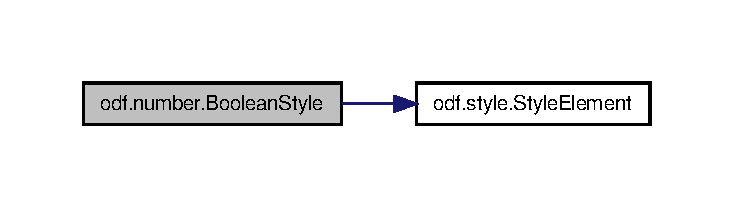
\includegraphics[width=350pt]{namespaceodf_1_1number_af5e0e7f6c98f62e21f0e71010f5aa563_cgraph}
\end{center}
\end{figure}


\hypertarget{namespaceodf_1_1number_ac6b4d66af1b244f0eb18d78e8e005e74}{\index{odf\+::number@{odf\+::number}!Currency\+Style@{Currency\+Style}}
\index{Currency\+Style@{Currency\+Style}!odf\+::number@{odf\+::number}}
\subsubsection[{Currency\+Style}]{\setlength{\rightskip}{0pt plus 5cm}def odf.\+number.\+Currency\+Style (
\begin{DoxyParamCaption}
\item[{}]{args}
\end{DoxyParamCaption}
)}}\label{namespaceodf_1_1number_ac6b4d66af1b244f0eb18d78e8e005e74}


Definition at line 36 of file number.\+py.



Here is the call graph for this function\+:
\nopagebreak
\begin{figure}[H]
\begin{center}
\leavevmode
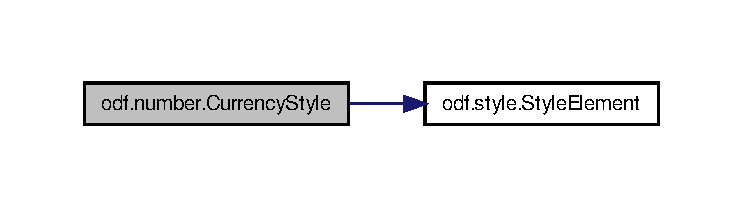
\includegraphics[width=350pt]{namespaceodf_1_1number_ac6b4d66af1b244f0eb18d78e8e005e74_cgraph}
\end{center}
\end{figure}


\hypertarget{namespaceodf_1_1number_a00794cb7b8d2fcc4d02abaf1779e71ae}{\index{odf\+::number@{odf\+::number}!Currency\+Symbol@{Currency\+Symbol}}
\index{Currency\+Symbol@{Currency\+Symbol}!odf\+::number@{odf\+::number}}
\subsubsection[{Currency\+Symbol}]{\setlength{\rightskip}{0pt plus 5cm}def odf.\+number.\+Currency\+Symbol (
\begin{DoxyParamCaption}
\item[{}]{args}
\end{DoxyParamCaption}
)}}\label{namespaceodf_1_1number_a00794cb7b8d2fcc4d02abaf1779e71ae}


Definition at line 39 of file number.\+py.

\hypertarget{namespaceodf_1_1number_ab42d20ae70cc68d268f68ddc16a1d149}{\index{odf\+::number@{odf\+::number}!Date\+Style@{Date\+Style}}
\index{Date\+Style@{Date\+Style}!odf\+::number@{odf\+::number}}
\subsubsection[{Date\+Style}]{\setlength{\rightskip}{0pt plus 5cm}def odf.\+number.\+Date\+Style (
\begin{DoxyParamCaption}
\item[{}]{args}
\end{DoxyParamCaption}
)}}\label{namespaceodf_1_1number_ab42d20ae70cc68d268f68ddc16a1d149}


Definition at line 42 of file number.\+py.



Here is the call graph for this function\+:
\nopagebreak
\begin{figure}[H]
\begin{center}
\leavevmode
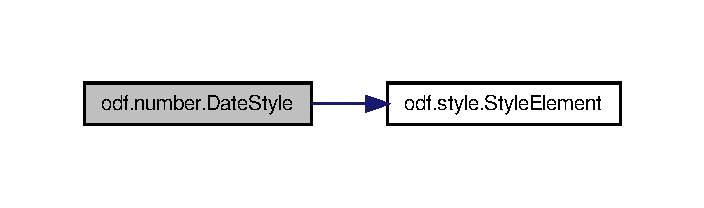
\includegraphics[width=338pt]{namespaceodf_1_1number_ab42d20ae70cc68d268f68ddc16a1d149_cgraph}
\end{center}
\end{figure}


\hypertarget{namespaceodf_1_1number_af55f319c7eadc936fc284fbe5fd38176}{\index{odf\+::number@{odf\+::number}!Day@{Day}}
\index{Day@{Day}!odf\+::number@{odf\+::number}}
\subsubsection[{Day}]{\setlength{\rightskip}{0pt plus 5cm}def odf.\+number.\+Day (
\begin{DoxyParamCaption}
\item[{}]{args}
\end{DoxyParamCaption}
)}}\label{namespaceodf_1_1number_af55f319c7eadc936fc284fbe5fd38176}


Definition at line 45 of file number.\+py.

\hypertarget{namespaceodf_1_1number_a91bde3f4fdaee80ac82101bce6b04e42}{\index{odf\+::number@{odf\+::number}!Day\+Of\+Week@{Day\+Of\+Week}}
\index{Day\+Of\+Week@{Day\+Of\+Week}!odf\+::number@{odf\+::number}}
\subsubsection[{Day\+Of\+Week}]{\setlength{\rightskip}{0pt plus 5cm}def odf.\+number.\+Day\+Of\+Week (
\begin{DoxyParamCaption}
\item[{}]{args}
\end{DoxyParamCaption}
)}}\label{namespaceodf_1_1number_a91bde3f4fdaee80ac82101bce6b04e42}


Definition at line 48 of file number.\+py.

\hypertarget{namespaceodf_1_1number_a584d0f2f580d89758a64c7a12cac00ba}{\index{odf\+::number@{odf\+::number}!Embedded\+Text@{Embedded\+Text}}
\index{Embedded\+Text@{Embedded\+Text}!odf\+::number@{odf\+::number}}
\subsubsection[{Embedded\+Text}]{\setlength{\rightskip}{0pt plus 5cm}def odf.\+number.\+Embedded\+Text (
\begin{DoxyParamCaption}
\item[{}]{args}
\end{DoxyParamCaption}
)}}\label{namespaceodf_1_1number_a584d0f2f580d89758a64c7a12cac00ba}


Definition at line 51 of file number.\+py.

\hypertarget{namespaceodf_1_1number_a5470f463bae52c7e0e6df56eb4b50f98}{\index{odf\+::number@{odf\+::number}!Era@{Era}}
\index{Era@{Era}!odf\+::number@{odf\+::number}}
\subsubsection[{Era}]{\setlength{\rightskip}{0pt plus 5cm}def odf.\+number.\+Era (
\begin{DoxyParamCaption}
\item[{}]{args}
\end{DoxyParamCaption}
)}}\label{namespaceodf_1_1number_a5470f463bae52c7e0e6df56eb4b50f98}


Definition at line 54 of file number.\+py.

\hypertarget{namespaceodf_1_1number_a75db68268c51f6d01055af520bd125a7}{\index{odf\+::number@{odf\+::number}!Fraction@{Fraction}}
\index{Fraction@{Fraction}!odf\+::number@{odf\+::number}}
\subsubsection[{Fraction}]{\setlength{\rightskip}{0pt plus 5cm}def odf.\+number.\+Fraction (
\begin{DoxyParamCaption}
\item[{}]{args}
\end{DoxyParamCaption}
)}}\label{namespaceodf_1_1number_a75db68268c51f6d01055af520bd125a7}


Definition at line 57 of file number.\+py.

\hypertarget{namespaceodf_1_1number_a68a3e593b38c22a4bcec37149452b9ef}{\index{odf\+::number@{odf\+::number}!Hours@{Hours}}
\index{Hours@{Hours}!odf\+::number@{odf\+::number}}
\subsubsection[{Hours}]{\setlength{\rightskip}{0pt plus 5cm}def odf.\+number.\+Hours (
\begin{DoxyParamCaption}
\item[{}]{args}
\end{DoxyParamCaption}
)}}\label{namespaceodf_1_1number_a68a3e593b38c22a4bcec37149452b9ef}


Definition at line 60 of file number.\+py.

\hypertarget{namespaceodf_1_1number_a6ec941c8ffd5ce304f089522b9963e09}{\index{odf\+::number@{odf\+::number}!Minutes@{Minutes}}
\index{Minutes@{Minutes}!odf\+::number@{odf\+::number}}
\subsubsection[{Minutes}]{\setlength{\rightskip}{0pt plus 5cm}def odf.\+number.\+Minutes (
\begin{DoxyParamCaption}
\item[{}]{args}
\end{DoxyParamCaption}
)}}\label{namespaceodf_1_1number_a6ec941c8ffd5ce304f089522b9963e09}


Definition at line 63 of file number.\+py.

\hypertarget{namespaceodf_1_1number_a98b22595051a38103bce0d8ff3ec6b31}{\index{odf\+::number@{odf\+::number}!Month@{Month}}
\index{Month@{Month}!odf\+::number@{odf\+::number}}
\subsubsection[{Month}]{\setlength{\rightskip}{0pt plus 5cm}def odf.\+number.\+Month (
\begin{DoxyParamCaption}
\item[{}]{args}
\end{DoxyParamCaption}
)}}\label{namespaceodf_1_1number_a98b22595051a38103bce0d8ff3ec6b31}


Definition at line 66 of file number.\+py.

\hypertarget{namespaceodf_1_1number_a8ef64aa6b0a897ee0126227ceb7b6347}{\index{odf\+::number@{odf\+::number}!Number@{Number}}
\index{Number@{Number}!odf\+::number@{odf\+::number}}
\subsubsection[{Number}]{\setlength{\rightskip}{0pt plus 5cm}def odf.\+number.\+Number (
\begin{DoxyParamCaption}
\item[{}]{args}
\end{DoxyParamCaption}
)}}\label{namespaceodf_1_1number_a8ef64aa6b0a897ee0126227ceb7b6347}


Definition at line 69 of file number.\+py.

\hypertarget{namespaceodf_1_1number_a3de4c489058b4321d042bcc04127dcb6}{\index{odf\+::number@{odf\+::number}!Number\+Style@{Number\+Style}}
\index{Number\+Style@{Number\+Style}!odf\+::number@{odf\+::number}}
\subsubsection[{Number\+Style}]{\setlength{\rightskip}{0pt plus 5cm}def odf.\+number.\+Number\+Style (
\begin{DoxyParamCaption}
\item[{}]{args}
\end{DoxyParamCaption}
)}}\label{namespaceodf_1_1number_a3de4c489058b4321d042bcc04127dcb6}


Definition at line 72 of file number.\+py.



Here is the call graph for this function\+:
\nopagebreak
\begin{figure}[H]
\begin{center}
\leavevmode
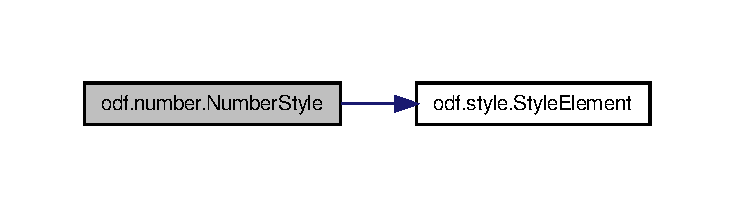
\includegraphics[width=350pt]{namespaceodf_1_1number_a3de4c489058b4321d042bcc04127dcb6_cgraph}
\end{center}
\end{figure}


\hypertarget{namespaceodf_1_1number_a2ceb4840095912a306db1c85e44e3fbd}{\index{odf\+::number@{odf\+::number}!Percentage\+Style@{Percentage\+Style}}
\index{Percentage\+Style@{Percentage\+Style}!odf\+::number@{odf\+::number}}
\subsubsection[{Percentage\+Style}]{\setlength{\rightskip}{0pt plus 5cm}def odf.\+number.\+Percentage\+Style (
\begin{DoxyParamCaption}
\item[{}]{args}
\end{DoxyParamCaption}
)}}\label{namespaceodf_1_1number_a2ceb4840095912a306db1c85e44e3fbd}


Definition at line 75 of file number.\+py.



Here is the call graph for this function\+:
\nopagebreak
\begin{figure}[H]
\begin{center}
\leavevmode
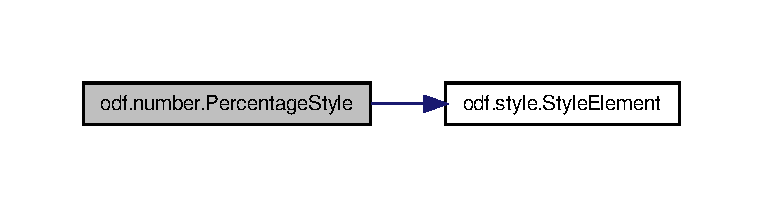
\includegraphics[width=350pt]{namespaceodf_1_1number_a2ceb4840095912a306db1c85e44e3fbd_cgraph}
\end{center}
\end{figure}


\hypertarget{namespaceodf_1_1number_ae824690a033450862c823cf1c8312351}{\index{odf\+::number@{odf\+::number}!Quarter@{Quarter}}
\index{Quarter@{Quarter}!odf\+::number@{odf\+::number}}
\subsubsection[{Quarter}]{\setlength{\rightskip}{0pt plus 5cm}def odf.\+number.\+Quarter (
\begin{DoxyParamCaption}
\item[{}]{args}
\end{DoxyParamCaption}
)}}\label{namespaceodf_1_1number_ae824690a033450862c823cf1c8312351}


Definition at line 78 of file number.\+py.

\hypertarget{namespaceodf_1_1number_a98c097e9c6b3ec73e715e46d1e4862a5}{\index{odf\+::number@{odf\+::number}!Scientific\+Number@{Scientific\+Number}}
\index{Scientific\+Number@{Scientific\+Number}!odf\+::number@{odf\+::number}}
\subsubsection[{Scientific\+Number}]{\setlength{\rightskip}{0pt plus 5cm}def odf.\+number.\+Scientific\+Number (
\begin{DoxyParamCaption}
\item[{}]{args}
\end{DoxyParamCaption}
)}}\label{namespaceodf_1_1number_a98c097e9c6b3ec73e715e46d1e4862a5}


Definition at line 81 of file number.\+py.

\hypertarget{namespaceodf_1_1number_a3da40292d59706edbb4358f3565f49ac}{\index{odf\+::number@{odf\+::number}!Seconds@{Seconds}}
\index{Seconds@{Seconds}!odf\+::number@{odf\+::number}}
\subsubsection[{Seconds}]{\setlength{\rightskip}{0pt plus 5cm}def odf.\+number.\+Seconds (
\begin{DoxyParamCaption}
\item[{}]{args}
\end{DoxyParamCaption}
)}}\label{namespaceodf_1_1number_a3da40292d59706edbb4358f3565f49ac}


Definition at line 84 of file number.\+py.

\hypertarget{namespaceodf_1_1number_a9858339662787da2aedfe7866d37d985}{\index{odf\+::number@{odf\+::number}!Text@{Text}}
\index{Text@{Text}!odf\+::number@{odf\+::number}}
\subsubsection[{Text}]{\setlength{\rightskip}{0pt plus 5cm}def odf.\+number.\+Text (
\begin{DoxyParamCaption}
\item[{}]{args}
\end{DoxyParamCaption}
)}}\label{namespaceodf_1_1number_a9858339662787da2aedfe7866d37d985}


Definition at line 87 of file number.\+py.

\hypertarget{namespaceodf_1_1number_a7cba65cb3ca91b979661a42716784157}{\index{odf\+::number@{odf\+::number}!Text\+Content@{Text\+Content}}
\index{Text\+Content@{Text\+Content}!odf\+::number@{odf\+::number}}
\subsubsection[{Text\+Content}]{\setlength{\rightskip}{0pt plus 5cm}def odf.\+number.\+Text\+Content (
\begin{DoxyParamCaption}
\item[{}]{args}
\end{DoxyParamCaption}
)}}\label{namespaceodf_1_1number_a7cba65cb3ca91b979661a42716784157}


Definition at line 90 of file number.\+py.

\hypertarget{namespaceodf_1_1number_a398c168b934489bcb746a51500b18e68}{\index{odf\+::number@{odf\+::number}!Text\+Style@{Text\+Style}}
\index{Text\+Style@{Text\+Style}!odf\+::number@{odf\+::number}}
\subsubsection[{Text\+Style}]{\setlength{\rightskip}{0pt plus 5cm}def odf.\+number.\+Text\+Style (
\begin{DoxyParamCaption}
\item[{}]{args}
\end{DoxyParamCaption}
)}}\label{namespaceodf_1_1number_a398c168b934489bcb746a51500b18e68}


Definition at line 93 of file number.\+py.



Here is the call graph for this function\+:
\nopagebreak
\begin{figure}[H]
\begin{center}
\leavevmode
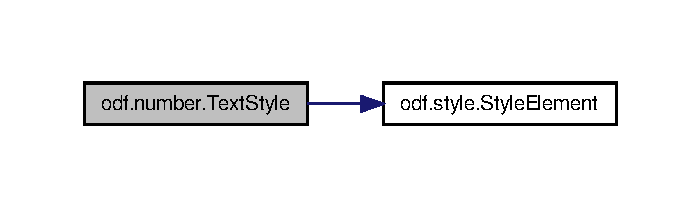
\includegraphics[width=336pt]{namespaceodf_1_1number_a398c168b934489bcb746a51500b18e68_cgraph}
\end{center}
\end{figure}


\hypertarget{namespaceodf_1_1number_a70598f014bbfd84e75a373c7a6eeaf22}{\index{odf\+::number@{odf\+::number}!Time\+Style@{Time\+Style}}
\index{Time\+Style@{Time\+Style}!odf\+::number@{odf\+::number}}
\subsubsection[{Time\+Style}]{\setlength{\rightskip}{0pt plus 5cm}def odf.\+number.\+Time\+Style (
\begin{DoxyParamCaption}
\item[{}]{args}
\end{DoxyParamCaption}
)}}\label{namespaceodf_1_1number_a70598f014bbfd84e75a373c7a6eeaf22}


Definition at line 96 of file number.\+py.



Here is the call graph for this function\+:
\nopagebreak
\begin{figure}[H]
\begin{center}
\leavevmode
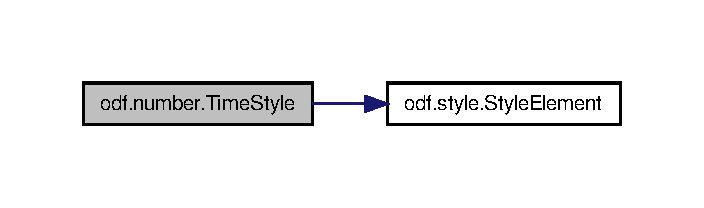
\includegraphics[width=338pt]{namespaceodf_1_1number_a70598f014bbfd84e75a373c7a6eeaf22_cgraph}
\end{center}
\end{figure}


\hypertarget{namespaceodf_1_1number_ae40b66fe193b0e4cdbf8a10d1122d83e}{\index{odf\+::number@{odf\+::number}!Week\+Of\+Year@{Week\+Of\+Year}}
\index{Week\+Of\+Year@{Week\+Of\+Year}!odf\+::number@{odf\+::number}}
\subsubsection[{Week\+Of\+Year}]{\setlength{\rightskip}{0pt plus 5cm}def odf.\+number.\+Week\+Of\+Year (
\begin{DoxyParamCaption}
\item[{}]{args}
\end{DoxyParamCaption}
)}}\label{namespaceodf_1_1number_ae40b66fe193b0e4cdbf8a10d1122d83e}


Definition at line 99 of file number.\+py.

\hypertarget{namespaceodf_1_1number_a94719cca5c80ecae146f23f07e6fe205}{\index{odf\+::number@{odf\+::number}!Year@{Year}}
\index{Year@{Year}!odf\+::number@{odf\+::number}}
\subsubsection[{Year}]{\setlength{\rightskip}{0pt plus 5cm}def odf.\+number.\+Year (
\begin{DoxyParamCaption}
\item[{}]{args}
\end{DoxyParamCaption}
)}}\label{namespaceodf_1_1number_a94719cca5c80ecae146f23f07e6fe205}


Definition at line 102 of file number.\+py.


\hypertarget{namespaceodf_1_1odf2moinmoin}{\section{odf.\+odf2moinmoin Namespace Reference}
\label{namespaceodf_1_1odf2moinmoin}\index{odf.\+odf2moinmoin@{odf.\+odf2moinmoin}}
}
\subsection*{Classes}
\begin{DoxyCompactItemize}
\item 
class \hyperlink{classodf_1_1odf2moinmoin_1_1ListProperties}{List\+Properties}
\begin{DoxyCompactList}\small\item\em Holds properties for a list style. \end{DoxyCompactList}\item 
class \hyperlink{classodf_1_1odf2moinmoin_1_1ODF2MoinMoin}{O\+D\+F2\+Moin\+Moin}
\item 
class \hyperlink{classodf_1_1odf2moinmoin_1_1ParagraphProps}{Paragraph\+Props}
\begin{DoxyCompactList}\small\item\em Holds properties of a paragraph style. \end{DoxyCompactList}\item 
class \hyperlink{classodf_1_1odf2moinmoin_1_1TextProps}{Text\+Props}
\begin{DoxyCompactList}\small\item\em Holds properties for a text style. \end{DoxyCompactList}\end{DoxyCompactItemize}
\subsection*{Variables}
\begin{DoxyCompactItemize}
\item 
list \hyperlink{namespaceodf_1_1odf2moinmoin_ae790cd24a0f06d818d0244c39006f0c4}{I\+G\+N\+O\+R\+E\+D\+\_\+\+T\+A\+G\+S}
\item 
list \hyperlink{namespaceodf_1_1odf2moinmoin_a0289a4d7cb05f857a7b043eacdbc4fcf}{I\+N\+L\+I\+N\+E\+\_\+\+T\+A\+G\+S} = \mbox{[} nsdict\mbox{[}item\mbox{[}0\mbox{]}\mbox{]}+\char`\"{}\+:\char`\"{}+item\mbox{[}1\mbox{]} for item in inline\+\_\+elements\mbox{]}
\end{DoxyCompactItemize}


\subsection{Variable Documentation}
\hypertarget{namespaceodf_1_1odf2moinmoin_ae790cd24a0f06d818d0244c39006f0c4}{\index{odf\+::odf2moinmoin@{odf\+::odf2moinmoin}!I\+G\+N\+O\+R\+E\+D\+\_\+\+T\+A\+G\+S@{I\+G\+N\+O\+R\+E\+D\+\_\+\+T\+A\+G\+S}}
\index{I\+G\+N\+O\+R\+E\+D\+\_\+\+T\+A\+G\+S@{I\+G\+N\+O\+R\+E\+D\+\_\+\+T\+A\+G\+S}!odf\+::odf2moinmoin@{odf\+::odf2moinmoin}}
\subsubsection[{I\+G\+N\+O\+R\+E\+D\+\_\+\+T\+A\+G\+S}]{\setlength{\rightskip}{0pt plus 5cm}list odf.\+odf2moinmoin.\+I\+G\+N\+O\+R\+E\+D\+\_\+\+T\+A\+G\+S}}\label{namespaceodf_1_1odf2moinmoin_ae790cd24a0f06d818d0244c39006f0c4}
{\bfseries Initial value\+:}
\begin{DoxyCode}
1 = [
2     \textcolor{stringliteral}{'draw:a'}
3     \textcolor{stringliteral}{'draw:g'},
4     \textcolor{stringliteral}{'draw:line'},
5     \textcolor{stringliteral}{'draw:object-ole'},
6     \textcolor{stringliteral}{'office:annotation'},
7     \textcolor{stringliteral}{'presentation:notes'},
8     \textcolor{stringliteral}{'svg:desc'},
9 ]
\end{DoxyCode}


Definition at line 27 of file odf2moinmoin.\+py.

\hypertarget{namespaceodf_1_1odf2moinmoin_a0289a4d7cb05f857a7b043eacdbc4fcf}{\index{odf\+::odf2moinmoin@{odf\+::odf2moinmoin}!I\+N\+L\+I\+N\+E\+\_\+\+T\+A\+G\+S@{I\+N\+L\+I\+N\+E\+\_\+\+T\+A\+G\+S}}
\index{I\+N\+L\+I\+N\+E\+\_\+\+T\+A\+G\+S@{I\+N\+L\+I\+N\+E\+\_\+\+T\+A\+G\+S}!odf\+::odf2moinmoin@{odf\+::odf2moinmoin}}
\subsubsection[{I\+N\+L\+I\+N\+E\+\_\+\+T\+A\+G\+S}]{\setlength{\rightskip}{0pt plus 5cm}list odf.\+odf2moinmoin.\+I\+N\+L\+I\+N\+E\+\_\+\+T\+A\+G\+S = \mbox{[} nsdict\mbox{[}item\mbox{[}0\mbox{]}\mbox{]}+\char`\"{}\+:\char`\"{}+item\mbox{[}1\mbox{]} for item in inline\+\_\+elements\mbox{]}}}\label{namespaceodf_1_1odf2moinmoin_a0289a4d7cb05f857a7b043eacdbc4fcf}


Definition at line 37 of file odf2moinmoin.\+py.


\hypertarget{namespaceodf_1_1odf2xhtml}{\section{odf.\+odf2xhtml Namespace Reference}
\label{namespaceodf_1_1odf2xhtml}\index{odf.\+odf2xhtml@{odf.\+odf2xhtml}}
}
\subsection*{Classes}
\begin{DoxyCompactItemize}
\item 
class \hyperlink{classodf_1_1odf2xhtml_1_1ODF2XHTML}{O\+D\+F2\+X\+H\+T\+M\+L}
\begin{DoxyCompactList}\small\item\em The \hyperlink{classodf_1_1odf2xhtml_1_1ODF2XHTML}{O\+D\+F2\+X\+H\+T\+M\+L} parses an O\+D\+F file and produces X\+H\+T\+M\+L. \end{DoxyCompactList}\item 
class \hyperlink{classodf_1_1odf2xhtml_1_1ODF2XHTMLembedded}{O\+D\+F2\+X\+H\+T\+M\+Lembedded}
\begin{DoxyCompactList}\small\item\em The \hyperlink{classodf_1_1odf2xhtml_1_1ODF2XHTML}{O\+D\+F2\+X\+H\+T\+M\+L} parses an O\+D\+F file and produces X\+H\+T\+M\+L. \end{DoxyCompactList}\item 
class \hyperlink{classodf_1_1odf2xhtml_1_1StyleToCSS}{Style\+To\+C\+S\+S}
\begin{DoxyCompactList}\small\item\em The purpose of the \hyperlink{classodf_1_1odf2xhtml_1_1StyleToCSS}{Style\+To\+C\+S\+S} class is to contain the rules to convert O\+D\+F styles to C\+S\+S2. \end{DoxyCompactList}\item 
class \hyperlink{classodf_1_1odf2xhtml_1_1TagStack}{Tag\+Stack}
\end{DoxyCompactItemize}
\subsection*{Variables}
\begin{DoxyCompactItemize}
\item 
dictionary \hyperlink{namespaceodf_1_1odf2xhtml_a45771f201b4cf26ab88c538306808fd7}{special\+\_\+styles}
\end{DoxyCompactItemize}


\subsection{Variable Documentation}
\hypertarget{namespaceodf_1_1odf2xhtml_a45771f201b4cf26ab88c538306808fd7}{\index{odf\+::odf2xhtml@{odf\+::odf2xhtml}!special\+\_\+styles@{special\+\_\+styles}}
\index{special\+\_\+styles@{special\+\_\+styles}!odf\+::odf2xhtml@{odf\+::odf2xhtml}}
\subsubsection[{special\+\_\+styles}]{\setlength{\rightskip}{0pt plus 5cm}dictionary odf.\+odf2xhtml.\+special\+\_\+styles}}\label{namespaceodf_1_1odf2xhtml_a45771f201b4cf26ab88c538306808fd7}
{\bfseries Initial value\+:}
\begin{DoxyCode}
1 = \{
2    \textcolor{stringliteral}{'S-Emphasis'}:\textcolor{stringliteral}{'em'},
3    \textcolor{stringliteral}{'S-Citation'}:\textcolor{stringliteral}{'cite'},
4    \textcolor{stringliteral}{'S-Strong\_20\_Emphasis'}:\textcolor{stringliteral}{'strong'},
5    \textcolor{stringliteral}{'S-Variable'}:\textcolor{stringliteral}{'var'},
6    \textcolor{stringliteral}{'S-Definition'}:\textcolor{stringliteral}{'dfn'},
7    \textcolor{stringliteral}{'S-Teletype'}:\textcolor{stringliteral}{'tt'},
8    \textcolor{stringliteral}{'P-Heading\_20\_1'}:\textcolor{stringliteral}{'h1'},
9    \textcolor{stringliteral}{'P-Heading\_20\_2'}:\textcolor{stringliteral}{'h2'},
10    \textcolor{stringliteral}{'P-Heading\_20\_3'}:\textcolor{stringliteral}{'h3'},
11    \textcolor{stringliteral}{'P-Heading\_20\_4'}:\textcolor{stringliteral}{'h4'},
12    \textcolor{stringliteral}{'P-Heading\_20\_5'}:\textcolor{stringliteral}{'h5'},
13    \textcolor{stringliteral}{'P-Heading\_20\_6'}:\textcolor{stringliteral}{'h6'},
14 \textcolor{comment}{#  'P-Caption':'caption',}
15    \textcolor{stringliteral}{'P-Addressee'}:\textcolor{stringliteral}{'address'},
16 \textcolor{comment}{#  'P-List\_20\_Heading':'dt',}
17 \textcolor{comment}{#  'P-List\_20\_Contents':'dd',}
18    \textcolor{stringliteral}{'P-Preformatted\_20\_Text'}:\textcolor{stringliteral}{'pre'},
19 \textcolor{comment}{#  'P-Table\_20\_Heading':'th',}
20 \textcolor{comment}{#  'P-Table\_20\_Contents':'td',}
21 \textcolor{comment}{#  'P-Text\_20\_body':'p'}
22 \}
\end{DoxyCode}


Definition at line 332 of file odf2xhtml.\+py.


\hypertarget{namespaceodf_1_1odfmanifest}{\section{odf.\+odfmanifest Namespace Reference}
\label{namespaceodf_1_1odfmanifest}\index{odf.\+odfmanifest@{odf.\+odfmanifest}}
}
\subsection*{Classes}
\begin{DoxyCompactItemize}
\item 
class \hyperlink{classodf_1_1odfmanifest_1_1ODFManifestHandler}{O\+D\+F\+Manifest\+Handler}
\begin{DoxyCompactList}\small\item\em The \hyperlink{classodf_1_1odfmanifest_1_1ODFManifestHandler}{O\+D\+F\+Manifest\+Handler} parses a manifest file and produces a list of content. \end{DoxyCompactList}\end{DoxyCompactItemize}
\subsection*{Functions}
\begin{DoxyCompactItemize}
\item 
def \hyperlink{namespaceodf_1_1odfmanifest_aa30e4aac456f93d3a2ec1d6eafd77004}{manifestlist}
\item 
def \hyperlink{namespaceodf_1_1odfmanifest_a69af946eb54c4a75e75cef5611d6fcef}{odfmanifest}
\end{DoxyCompactItemize}
\subsection*{Variables}
\begin{DoxyCompactItemize}
\item 
string \hyperlink{namespaceodf_1_1odfmanifest_a66286c05d5031965957b26b57b7bbfbd}{M\+A\+N\+I\+F\+E\+S\+T\+N\+S} = \char`\"{}urn\+:oasis\+:names\+:tc\+:opendocument\+:xmlns\+:manifest\+:1.\+0\char`\"{}
\item 
tuple \hyperlink{namespaceodf_1_1odfmanifest_a1641ce31eefa41ae260f4bd5785b37b3}{result} = \hyperlink{namespaceodf_1_1odfmanifest_a69af946eb54c4a75e75cef5611d6fcef}{odfmanifest}(sys.\+argv\mbox{[}1\mbox{]})
\end{DoxyCompactItemize}


\subsection{Function Documentation}
\hypertarget{namespaceodf_1_1odfmanifest_aa30e4aac456f93d3a2ec1d6eafd77004}{\index{odf\+::odfmanifest@{odf\+::odfmanifest}!manifestlist@{manifestlist}}
\index{manifestlist@{manifestlist}!odf\+::odfmanifest@{odf\+::odfmanifest}}
\subsubsection[{manifestlist}]{\setlength{\rightskip}{0pt plus 5cm}def odf.\+odfmanifest.\+manifestlist (
\begin{DoxyParamCaption}
\item[{}]{manifestxml}
\end{DoxyParamCaption}
)}}\label{namespaceodf_1_1odfmanifest_aa30e4aac456f93d3a2ec1d6eafd77004}


Definition at line 95 of file odfmanifest.\+py.



Here is the caller graph for this function\+:
\nopagebreak
\begin{figure}[H]
\begin{center}
\leavevmode
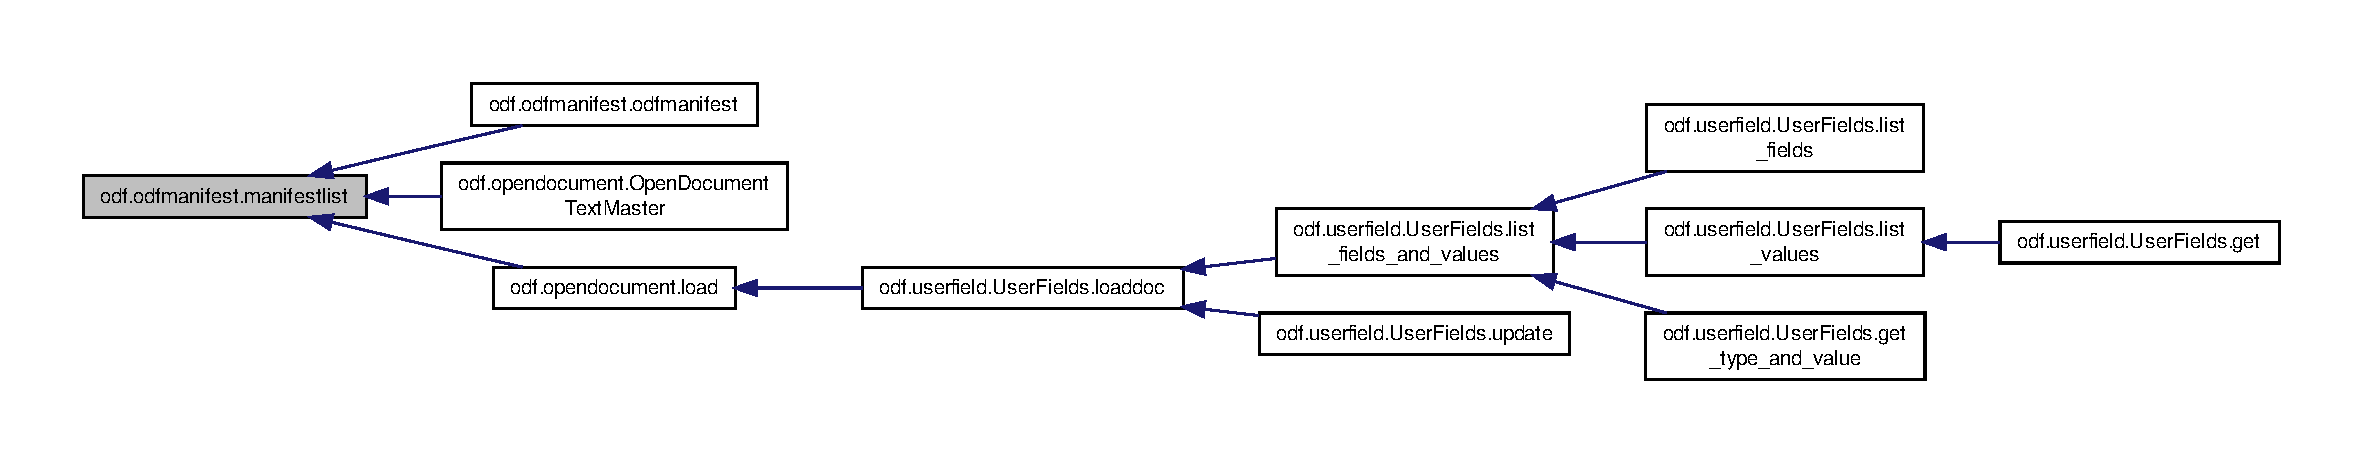
\includegraphics[width=350pt]{namespaceodf_1_1odfmanifest_aa30e4aac456f93d3a2ec1d6eafd77004_icgraph}
\end{center}
\end{figure}


\hypertarget{namespaceodf_1_1odfmanifest_a69af946eb54c4a75e75cef5611d6fcef}{\index{odf\+::odfmanifest@{odf\+::odfmanifest}!odfmanifest@{odfmanifest}}
\index{odfmanifest@{odfmanifest}!odf\+::odfmanifest@{odf\+::odfmanifest}}
\subsubsection[{odfmanifest}]{\setlength{\rightskip}{0pt plus 5cm}def odf.\+odfmanifest.\+odfmanifest (
\begin{DoxyParamCaption}
\item[{}]{odtfile}
\end{DoxyParamCaption}
)}}\label{namespaceodf_1_1odfmanifest_a69af946eb54c4a75e75cef5611d6fcef}


Definition at line 110 of file odfmanifest.\+py.



Here is the call graph for this function\+:
\nopagebreak
\begin{figure}[H]
\begin{center}
\leavevmode
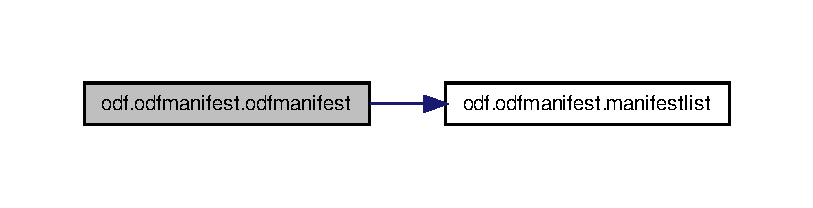
\includegraphics[width=350pt]{namespaceodf_1_1odfmanifest_a69af946eb54c4a75e75cef5611d6fcef_cgraph}
\end{center}
\end{figure}




\subsection{Variable Documentation}
\hypertarget{namespaceodf_1_1odfmanifest_a66286c05d5031965957b26b57b7bbfbd}{\index{odf\+::odfmanifest@{odf\+::odfmanifest}!M\+A\+N\+I\+F\+E\+S\+T\+N\+S@{M\+A\+N\+I\+F\+E\+S\+T\+N\+S}}
\index{M\+A\+N\+I\+F\+E\+S\+T\+N\+S@{M\+A\+N\+I\+F\+E\+S\+T\+N\+S}!odf\+::odfmanifest@{odf\+::odfmanifest}}
\subsubsection[{M\+A\+N\+I\+F\+E\+S\+T\+N\+S}]{\setlength{\rightskip}{0pt plus 5cm}string odf.\+odfmanifest.\+M\+A\+N\+I\+F\+E\+S\+T\+N\+S = \char`\"{}urn\+:oasis\+:names\+:tc\+:opendocument\+:xmlns\+:manifest\+:1.\+0\char`\"{}}}\label{namespaceodf_1_1odfmanifest_a66286c05d5031965957b26b57b7bbfbd}


Definition at line 32 of file odfmanifest.\+py.

\hypertarget{namespaceodf_1_1odfmanifest_a1641ce31eefa41ae260f4bd5785b37b3}{\index{odf\+::odfmanifest@{odf\+::odfmanifest}!result@{result}}
\index{result@{result}!odf\+::odfmanifest@{odf\+::odfmanifest}}
\subsubsection[{result}]{\setlength{\rightskip}{0pt plus 5cm}tuple odf.\+odfmanifest.\+result = {\bf odfmanifest}(sys.\+argv\mbox{[}1\mbox{]})}}\label{namespaceodf_1_1odfmanifest_a1641ce31eefa41ae260f4bd5785b37b3}


Definition at line 118 of file odfmanifest.\+py.


\hypertarget{namespaceodf_1_1office}{\section{odf.\+office Namespace Reference}
\label{namespaceodf_1_1office}\index{odf.\+office@{odf.\+office}}
}
\subsection*{Functions}
\begin{DoxyCompactItemize}
\item 
def \hyperlink{namespaceodf_1_1office_a04497efb1d2eb04f1160a785801bd1ea}{Annotation}
\item 
def \hyperlink{namespaceodf_1_1office_a03f599b1065c597dccff9a79d841e8f2}{Annotation\+End}
\item 
def \hyperlink{namespaceodf_1_1office_abcd765298646e8cd782dbca186afe6b5}{Automatic\+Styles}
\item 
def \hyperlink{namespaceodf_1_1office_a1ffd116c8222f628c1aa249849be0ea1}{Binary\+Data}
\item 
def \hyperlink{namespaceodf_1_1office_af99bd1bdb6e0c44e5844977632ae767f}{Body}
\item 
def \hyperlink{namespaceodf_1_1office_a245fa42c280a2ddbcc5ab656cb6587bb}{Change\+Info}
\item 
def \hyperlink{namespaceodf_1_1office_af0b1c3c239d01f008cb2c6d4fc3240fb}{Chart}
\item 
def \hyperlink{namespaceodf_1_1office_ae9e3a5e7827329874bb5983127e5e97e}{Dde\+Source}
\item 
def \hyperlink{namespaceodf_1_1office_a8911e083995dcd8e4e79e9b3859df146}{Document}
\item 
def \hyperlink{namespaceodf_1_1office_a55094c9d071beb272023c7bddff88a03}{Document\+Content}
\item 
def \hyperlink{namespaceodf_1_1office_a897ebe1e7d3d9d00bf294b3ff0e827bd}{Document\+Meta}
\item 
def \hyperlink{namespaceodf_1_1office_a024d9cff5f35af20e1b2619fcc4ef797}{Document\+Settings}
\item 
def \hyperlink{namespaceodf_1_1office_abebbacc9a8bcd23644f3dc2ac7ff8129}{Document\+Styles}
\item 
def \hyperlink{namespaceodf_1_1office_a4243dc5ed97e8dd14f28f466710f67f3}{Drawing}
\item 
def \hyperlink{namespaceodf_1_1office_af4ef9b9abd30debca5bde6998c52df38}{Event\+Listeners}
\item 
def \hyperlink{namespaceodf_1_1office_a10ec2b7fabe2b0cf7737154b673f431f}{Font\+Face\+Decls}
\item 
def \hyperlink{namespaceodf_1_1office_a7e5036d213f81946d74782122b0549b7}{Forms}
\item 
def \hyperlink{namespaceodf_1_1office_af85f6bb35682d9491279f80eff51f77d}{Image}
\item 
def \hyperlink{namespaceodf_1_1office_a151528d5a05134adfc3ed80cccfe500d}{Master\+Styles}
\item 
def \hyperlink{namespaceodf_1_1office_add28fb40129e830ffcd2a45a720201da}{Meta}
\item 
def \hyperlink{namespaceodf_1_1office_a60bdb5eb3929beaded4ac63454d4b7e0}{Presentation}
\item 
def \hyperlink{namespaceodf_1_1office_aafe3a73ef2d735377745e772217173e8}{Script}
\item 
def \hyperlink{namespaceodf_1_1office_ac7074ce39032dcd9caa4d8996efa1d9b}{Scripts}
\item 
def \hyperlink{namespaceodf_1_1office_a5a2c1261a69a9c9fa9772f09aa4b28b0}{Settings}
\item 
def \hyperlink{namespaceodf_1_1office_a6ddbb3918994609b625c6e2ade816540}{Spreadsheet}
\item 
def \hyperlink{namespaceodf_1_1office_a2e4051901a771cd9df62fc354bcce9bd}{Styles}
\item 
def \hyperlink{namespaceodf_1_1office_a8755db7dce4c0a1aaec54aa797b1a4da}{Text}
\end{DoxyCompactItemize}


\subsection{Function Documentation}
\hypertarget{namespaceodf_1_1office_a04497efb1d2eb04f1160a785801bd1ea}{\index{odf\+::office@{odf\+::office}!Annotation@{Annotation}}
\index{Annotation@{Annotation}!odf\+::office@{odf\+::office}}
\subsubsection[{Annotation}]{\setlength{\rightskip}{0pt plus 5cm}def odf.\+office.\+Annotation (
\begin{DoxyParamCaption}
\item[{}]{args}
\end{DoxyParamCaption}
)}}\label{namespaceodf_1_1office_a04497efb1d2eb04f1160a785801bd1ea}


Definition at line 26 of file office.\+py.



Here is the call graph for this function\+:
\nopagebreak
\begin{figure}[H]
\begin{center}
\leavevmode
\includegraphics[width=348pt]{namespaceodf_1_1office_a04497efb1d2eb04f1160a785801bd1ea_cgraph}
\end{center}
\end{figure}


\hypertarget{namespaceodf_1_1office_a03f599b1065c597dccff9a79d841e8f2}{\index{odf\+::office@{odf\+::office}!Annotation\+End@{Annotation\+End}}
\index{Annotation\+End@{Annotation\+End}!odf\+::office@{odf\+::office}}
\subsubsection[{Annotation\+End}]{\setlength{\rightskip}{0pt plus 5cm}def odf.\+office.\+Annotation\+End (
\begin{DoxyParamCaption}
\item[{}]{args}
\end{DoxyParamCaption}
)}}\label{namespaceodf_1_1office_a03f599b1065c597dccff9a79d841e8f2}


Definition at line 29 of file office.\+py.



Here is the call graph for this function\+:
\nopagebreak
\begin{figure}[H]
\begin{center}
\leavevmode
\includegraphics[width=350pt]{namespaceodf_1_1office_a03f599b1065c597dccff9a79d841e8f2_cgraph}
\end{center}
\end{figure}


\hypertarget{namespaceodf_1_1office_abcd765298646e8cd782dbca186afe6b5}{\index{odf\+::office@{odf\+::office}!Automatic\+Styles@{Automatic\+Styles}}
\index{Automatic\+Styles@{Automatic\+Styles}!odf\+::office@{odf\+::office}}
\subsubsection[{Automatic\+Styles}]{\setlength{\rightskip}{0pt plus 5cm}def odf.\+office.\+Automatic\+Styles (
\begin{DoxyParamCaption}
\item[{}]{args}
\end{DoxyParamCaption}
)}}\label{namespaceodf_1_1office_abcd765298646e8cd782dbca186afe6b5}


Definition at line 32 of file office.\+py.



Here is the caller graph for this function\+:
\nopagebreak
\begin{figure}[H]
\begin{center}
\leavevmode
\includegraphics[width=350pt]{namespaceodf_1_1office_abcd765298646e8cd782dbca186afe6b5_icgraph}
\end{center}
\end{figure}


\hypertarget{namespaceodf_1_1office_a1ffd116c8222f628c1aa249849be0ea1}{\index{odf\+::office@{odf\+::office}!Binary\+Data@{Binary\+Data}}
\index{Binary\+Data@{Binary\+Data}!odf\+::office@{odf\+::office}}
\subsubsection[{Binary\+Data}]{\setlength{\rightskip}{0pt plus 5cm}def odf.\+office.\+Binary\+Data (
\begin{DoxyParamCaption}
\item[{}]{args}
\end{DoxyParamCaption}
)}}\label{namespaceodf_1_1office_a1ffd116c8222f628c1aa249849be0ea1}


Definition at line 35 of file office.\+py.

\hypertarget{namespaceodf_1_1office_af99bd1bdb6e0c44e5844977632ae767f}{\index{odf\+::office@{odf\+::office}!Body@{Body}}
\index{Body@{Body}!odf\+::office@{odf\+::office}}
\subsubsection[{Body}]{\setlength{\rightskip}{0pt plus 5cm}def odf.\+office.\+Body (
\begin{DoxyParamCaption}
\item[{}]{args}
\end{DoxyParamCaption}
)}}\label{namespaceodf_1_1office_af99bd1bdb6e0c44e5844977632ae767f}


Definition at line 38 of file office.\+py.

\hypertarget{namespaceodf_1_1office_a245fa42c280a2ddbcc5ab656cb6587bb}{\index{odf\+::office@{odf\+::office}!Change\+Info@{Change\+Info}}
\index{Change\+Info@{Change\+Info}!odf\+::office@{odf\+::office}}
\subsubsection[{Change\+Info}]{\setlength{\rightskip}{0pt plus 5cm}def odf.\+office.\+Change\+Info (
\begin{DoxyParamCaption}
\item[{}]{args}
\end{DoxyParamCaption}
)}}\label{namespaceodf_1_1office_a245fa42c280a2ddbcc5ab656cb6587bb}


Definition at line 41 of file office.\+py.

\hypertarget{namespaceodf_1_1office_af0b1c3c239d01f008cb2c6d4fc3240fb}{\index{odf\+::office@{odf\+::office}!Chart@{Chart}}
\index{Chart@{Chart}!odf\+::office@{odf\+::office}}
\subsubsection[{Chart}]{\setlength{\rightskip}{0pt plus 5cm}def odf.\+office.\+Chart (
\begin{DoxyParamCaption}
\item[{}]{args}
\end{DoxyParamCaption}
)}}\label{namespaceodf_1_1office_af0b1c3c239d01f008cb2c6d4fc3240fb}


Definition at line 44 of file office.\+py.

\hypertarget{namespaceodf_1_1office_ae9e3a5e7827329874bb5983127e5e97e}{\index{odf\+::office@{odf\+::office}!Dde\+Source@{Dde\+Source}}
\index{Dde\+Source@{Dde\+Source}!odf\+::office@{odf\+::office}}
\subsubsection[{Dde\+Source}]{\setlength{\rightskip}{0pt plus 5cm}def odf.\+office.\+Dde\+Source (
\begin{DoxyParamCaption}
\item[{}]{args}
\end{DoxyParamCaption}
)}}\label{namespaceodf_1_1office_ae9e3a5e7827329874bb5983127e5e97e}


Definition at line 47 of file office.\+py.

\hypertarget{namespaceodf_1_1office_a8911e083995dcd8e4e79e9b3859df146}{\index{odf\+::office@{odf\+::office}!Document@{Document}}
\index{Document@{Document}!odf\+::office@{odf\+::office}}
\subsubsection[{Document}]{\setlength{\rightskip}{0pt plus 5cm}def odf.\+office.\+Document (
\begin{DoxyParamCaption}
\item[{}]{version = {\ttfamily \char`\"{}1.2\char`\"{}}, }
\item[{}]{args}
\end{DoxyParamCaption}
)}}\label{namespaceodf_1_1office_a8911e083995dcd8e4e79e9b3859df146}


Definition at line 50 of file office.\+py.

\hypertarget{namespaceodf_1_1office_a55094c9d071beb272023c7bddff88a03}{\index{odf\+::office@{odf\+::office}!Document\+Content@{Document\+Content}}
\index{Document\+Content@{Document\+Content}!odf\+::office@{odf\+::office}}
\subsubsection[{Document\+Content}]{\setlength{\rightskip}{0pt plus 5cm}def odf.\+office.\+Document\+Content (
\begin{DoxyParamCaption}
\item[{}]{version = {\ttfamily \char`\"{}1.2\char`\"{}}, }
\item[{}]{args}
\end{DoxyParamCaption}
)}}\label{namespaceodf_1_1office_a55094c9d071beb272023c7bddff88a03}


Definition at line 53 of file office.\+py.



Here is the caller graph for this function\+:
\nopagebreak
\begin{figure}[H]
\begin{center}
\leavevmode
\includegraphics[width=350pt]{namespaceodf_1_1office_a55094c9d071beb272023c7bddff88a03_icgraph}
\end{center}
\end{figure}


\hypertarget{namespaceodf_1_1office_a897ebe1e7d3d9d00bf294b3ff0e827bd}{\index{odf\+::office@{odf\+::office}!Document\+Meta@{Document\+Meta}}
\index{Document\+Meta@{Document\+Meta}!odf\+::office@{odf\+::office}}
\subsubsection[{Document\+Meta}]{\setlength{\rightskip}{0pt plus 5cm}def odf.\+office.\+Document\+Meta (
\begin{DoxyParamCaption}
\item[{}]{version = {\ttfamily \char`\"{}1.2\char`\"{}}, }
\item[{}]{args}
\end{DoxyParamCaption}
)}}\label{namespaceodf_1_1office_a897ebe1e7d3d9d00bf294b3ff0e827bd}


Definition at line 56 of file office.\+py.



Here is the caller graph for this function\+:
\nopagebreak
\begin{figure}[H]
\begin{center}
\leavevmode
\includegraphics[width=350pt]{namespaceodf_1_1office_a897ebe1e7d3d9d00bf294b3ff0e827bd_icgraph}
\end{center}
\end{figure}


\hypertarget{namespaceodf_1_1office_a024d9cff5f35af20e1b2619fcc4ef797}{\index{odf\+::office@{odf\+::office}!Document\+Settings@{Document\+Settings}}
\index{Document\+Settings@{Document\+Settings}!odf\+::office@{odf\+::office}}
\subsubsection[{Document\+Settings}]{\setlength{\rightskip}{0pt plus 5cm}def odf.\+office.\+Document\+Settings (
\begin{DoxyParamCaption}
\item[{}]{version = {\ttfamily \char`\"{}1.2\char`\"{}}, }
\item[{}]{args}
\end{DoxyParamCaption}
)}}\label{namespaceodf_1_1office_a024d9cff5f35af20e1b2619fcc4ef797}


Definition at line 59 of file office.\+py.



Here is the caller graph for this function\+:
\nopagebreak
\begin{figure}[H]
\begin{center}
\leavevmode
\includegraphics[width=350pt]{namespaceodf_1_1office_a024d9cff5f35af20e1b2619fcc4ef797_icgraph}
\end{center}
\end{figure}


\hypertarget{namespaceodf_1_1office_abebbacc9a8bcd23644f3dc2ac7ff8129}{\index{odf\+::office@{odf\+::office}!Document\+Styles@{Document\+Styles}}
\index{Document\+Styles@{Document\+Styles}!odf\+::office@{odf\+::office}}
\subsubsection[{Document\+Styles}]{\setlength{\rightskip}{0pt plus 5cm}def odf.\+office.\+Document\+Styles (
\begin{DoxyParamCaption}
\item[{}]{version = {\ttfamily \char`\"{}1.2\char`\"{}}, }
\item[{}]{args}
\end{DoxyParamCaption}
)}}\label{namespaceodf_1_1office_abebbacc9a8bcd23644f3dc2ac7ff8129}


Definition at line 62 of file office.\+py.



Here is the caller graph for this function\+:
\nopagebreak
\begin{figure}[H]
\begin{center}
\leavevmode
\includegraphics[width=350pt]{namespaceodf_1_1office_abebbacc9a8bcd23644f3dc2ac7ff8129_icgraph}
\end{center}
\end{figure}


\hypertarget{namespaceodf_1_1office_a4243dc5ed97e8dd14f28f466710f67f3}{\index{odf\+::office@{odf\+::office}!Drawing@{Drawing}}
\index{Drawing@{Drawing}!odf\+::office@{odf\+::office}}
\subsubsection[{Drawing}]{\setlength{\rightskip}{0pt plus 5cm}def odf.\+office.\+Drawing (
\begin{DoxyParamCaption}
\item[{}]{args}
\end{DoxyParamCaption}
)}}\label{namespaceodf_1_1office_a4243dc5ed97e8dd14f28f466710f67f3}


Definition at line 65 of file office.\+py.



Here is the caller graph for this function\+:
\nopagebreak
\begin{figure}[H]
\begin{center}
\leavevmode
\includegraphics[width=350pt]{namespaceodf_1_1office_a4243dc5ed97e8dd14f28f466710f67f3_icgraph}
\end{center}
\end{figure}


\hypertarget{namespaceodf_1_1office_af4ef9b9abd30debca5bde6998c52df38}{\index{odf\+::office@{odf\+::office}!Event\+Listeners@{Event\+Listeners}}
\index{Event\+Listeners@{Event\+Listeners}!odf\+::office@{odf\+::office}}
\subsubsection[{Event\+Listeners}]{\setlength{\rightskip}{0pt plus 5cm}def odf.\+office.\+Event\+Listeners (
\begin{DoxyParamCaption}
\item[{}]{args}
\end{DoxyParamCaption}
)}}\label{namespaceodf_1_1office_af4ef9b9abd30debca5bde6998c52df38}


Definition at line 68 of file office.\+py.

\hypertarget{namespaceodf_1_1office_a10ec2b7fabe2b0cf7737154b673f431f}{\index{odf\+::office@{odf\+::office}!Font\+Face\+Decls@{Font\+Face\+Decls}}
\index{Font\+Face\+Decls@{Font\+Face\+Decls}!odf\+::office@{odf\+::office}}
\subsubsection[{Font\+Face\+Decls}]{\setlength{\rightskip}{0pt plus 5cm}def odf.\+office.\+Font\+Face\+Decls (
\begin{DoxyParamCaption}
\item[{}]{args}
\end{DoxyParamCaption}
)}}\label{namespaceodf_1_1office_a10ec2b7fabe2b0cf7737154b673f431f}


Definition at line 71 of file office.\+py.

\hypertarget{namespaceodf_1_1office_a7e5036d213f81946d74782122b0549b7}{\index{odf\+::office@{odf\+::office}!Forms@{Forms}}
\index{Forms@{Forms}!odf\+::office@{odf\+::office}}
\subsubsection[{Forms}]{\setlength{\rightskip}{0pt plus 5cm}def odf.\+office.\+Forms (
\begin{DoxyParamCaption}
\item[{}]{args}
\end{DoxyParamCaption}
)}}\label{namespaceodf_1_1office_a7e5036d213f81946d74782122b0549b7}


Definition at line 74 of file office.\+py.

\hypertarget{namespaceodf_1_1office_af85f6bb35682d9491279f80eff51f77d}{\index{odf\+::office@{odf\+::office}!Image@{Image}}
\index{Image@{Image}!odf\+::office@{odf\+::office}}
\subsubsection[{Image}]{\setlength{\rightskip}{0pt plus 5cm}def odf.\+office.\+Image (
\begin{DoxyParamCaption}
\item[{}]{args}
\end{DoxyParamCaption}
)}}\label{namespaceodf_1_1office_af85f6bb35682d9491279f80eff51f77d}


Definition at line 77 of file office.\+py.

\hypertarget{namespaceodf_1_1office_a151528d5a05134adfc3ed80cccfe500d}{\index{odf\+::office@{odf\+::office}!Master\+Styles@{Master\+Styles}}
\index{Master\+Styles@{Master\+Styles}!odf\+::office@{odf\+::office}}
\subsubsection[{Master\+Styles}]{\setlength{\rightskip}{0pt plus 5cm}def odf.\+office.\+Master\+Styles (
\begin{DoxyParamCaption}
\item[{}]{args}
\end{DoxyParamCaption}
)}}\label{namespaceodf_1_1office_a151528d5a05134adfc3ed80cccfe500d}


Definition at line 80 of file office.\+py.

\hypertarget{namespaceodf_1_1office_add28fb40129e830ffcd2a45a720201da}{\index{odf\+::office@{odf\+::office}!Meta@{Meta}}
\index{Meta@{Meta}!odf\+::office@{odf\+::office}}
\subsubsection[{Meta}]{\setlength{\rightskip}{0pt plus 5cm}def odf.\+office.\+Meta (
\begin{DoxyParamCaption}
\item[{}]{args}
\end{DoxyParamCaption}
)}}\label{namespaceodf_1_1office_add28fb40129e830ffcd2a45a720201da}


Definition at line 83 of file office.\+py.

\hypertarget{namespaceodf_1_1office_a60bdb5eb3929beaded4ac63454d4b7e0}{\index{odf\+::office@{odf\+::office}!Presentation@{Presentation}}
\index{Presentation@{Presentation}!odf\+::office@{odf\+::office}}
\subsubsection[{Presentation}]{\setlength{\rightskip}{0pt plus 5cm}def odf.\+office.\+Presentation (
\begin{DoxyParamCaption}
\item[{}]{args}
\end{DoxyParamCaption}
)}}\label{namespaceodf_1_1office_a60bdb5eb3929beaded4ac63454d4b7e0}


Definition at line 86 of file office.\+py.



Here is the caller graph for this function\+:
\nopagebreak
\begin{figure}[H]
\begin{center}
\leavevmode
\includegraphics[width=350pt]{namespaceodf_1_1office_a60bdb5eb3929beaded4ac63454d4b7e0_icgraph}
\end{center}
\end{figure}


\hypertarget{namespaceodf_1_1office_aafe3a73ef2d735377745e772217173e8}{\index{odf\+::office@{odf\+::office}!Script@{Script}}
\index{Script@{Script}!odf\+::office@{odf\+::office}}
\subsubsection[{Script}]{\setlength{\rightskip}{0pt plus 5cm}def odf.\+office.\+Script (
\begin{DoxyParamCaption}
\item[{}]{args}
\end{DoxyParamCaption}
)}}\label{namespaceodf_1_1office_aafe3a73ef2d735377745e772217173e8}


Definition at line 89 of file office.\+py.

\hypertarget{namespaceodf_1_1office_ac7074ce39032dcd9caa4d8996efa1d9b}{\index{odf\+::office@{odf\+::office}!Scripts@{Scripts}}
\index{Scripts@{Scripts}!odf\+::office@{odf\+::office}}
\subsubsection[{Scripts}]{\setlength{\rightskip}{0pt plus 5cm}def odf.\+office.\+Scripts (
\begin{DoxyParamCaption}
\item[{}]{args}
\end{DoxyParamCaption}
)}}\label{namespaceodf_1_1office_ac7074ce39032dcd9caa4d8996efa1d9b}


Definition at line 92 of file office.\+py.

\hypertarget{namespaceodf_1_1office_a5a2c1261a69a9c9fa9772f09aa4b28b0}{\index{odf\+::office@{odf\+::office}!Settings@{Settings}}
\index{Settings@{Settings}!odf\+::office@{odf\+::office}}
\subsubsection[{Settings}]{\setlength{\rightskip}{0pt plus 5cm}def odf.\+office.\+Settings (
\begin{DoxyParamCaption}
\item[{}]{args}
\end{DoxyParamCaption}
)}}\label{namespaceodf_1_1office_a5a2c1261a69a9c9fa9772f09aa4b28b0}


Definition at line 95 of file office.\+py.

\hypertarget{namespaceodf_1_1office_a6ddbb3918994609b625c6e2ade816540}{\index{odf\+::office@{odf\+::office}!Spreadsheet@{Spreadsheet}}
\index{Spreadsheet@{Spreadsheet}!odf\+::office@{odf\+::office}}
\subsubsection[{Spreadsheet}]{\setlength{\rightskip}{0pt plus 5cm}def odf.\+office.\+Spreadsheet (
\begin{DoxyParamCaption}
\item[{}]{args}
\end{DoxyParamCaption}
)}}\label{namespaceodf_1_1office_a6ddbb3918994609b625c6e2ade816540}


Definition at line 98 of file office.\+py.



Here is the caller graph for this function\+:
\nopagebreak
\begin{figure}[H]
\begin{center}
\leavevmode
\includegraphics[width=350pt]{namespaceodf_1_1office_a6ddbb3918994609b625c6e2ade816540_icgraph}
\end{center}
\end{figure}


\hypertarget{namespaceodf_1_1office_a2e4051901a771cd9df62fc354bcce9bd}{\index{odf\+::office@{odf\+::office}!Styles@{Styles}}
\index{Styles@{Styles}!odf\+::office@{odf\+::office}}
\subsubsection[{Styles}]{\setlength{\rightskip}{0pt plus 5cm}def odf.\+office.\+Styles (
\begin{DoxyParamCaption}
\item[{}]{args}
\end{DoxyParamCaption}
)}}\label{namespaceodf_1_1office_a2e4051901a771cd9df62fc354bcce9bd}


Definition at line 101 of file office.\+py.

\hypertarget{namespaceodf_1_1office_a8755db7dce4c0a1aaec54aa797b1a4da}{\index{odf\+::office@{odf\+::office}!Text@{Text}}
\index{Text@{Text}!odf\+::office@{odf\+::office}}
\subsubsection[{Text}]{\setlength{\rightskip}{0pt plus 5cm}def odf.\+office.\+Text (
\begin{DoxyParamCaption}
\item[{}]{args}
\end{DoxyParamCaption}
)}}\label{namespaceodf_1_1office_a8755db7dce4c0a1aaec54aa797b1a4da}


Definition at line 104 of file office.\+py.


\hypertarget{namespaceodf_1_1opendocument}{\section{odf.\+opendocument Namespace Reference}
\label{namespaceodf_1_1opendocument}\index{odf.\+opendocument@{odf.\+opendocument}}
}
\subsection*{Classes}
\begin{DoxyCompactItemize}
\item 
class \hyperlink{classodf_1_1opendocument_1_1OpaqueObject}{Opaque\+Object}
\begin{DoxyCompactList}\small\item\em just a record to bear a filename, a mediatype and a bytes content \end{DoxyCompactList}\item 
class \hyperlink{classodf_1_1opendocument_1_1OpenDocument}{Open\+Document}
\begin{DoxyCompactList}\small\item\em A class to hold the content of an \hyperlink{classodf_1_1opendocument_1_1OpenDocument}{Open\+Document} document Use the xml method to write the X\+M\+L source to the screen or to a file. \end{DoxyCompactList}\end{DoxyCompactItemize}
\subsection*{Functions}
\begin{DoxyCompactItemize}
\item 
def \hyperlink{namespaceodf_1_1opendocument_a6a86bb2e0369feaea53b7c05290b2392}{Open\+Document\+Chart}
\begin{DoxyCompactList}\small\item\em Creates a chart document. \end{DoxyCompactList}\item 
def \hyperlink{namespaceodf_1_1opendocument_a5ff2aeb89ca9dfbae829ee5853c7b3e2}{Open\+Document\+Drawing}
\begin{DoxyCompactList}\small\item\em Creates a drawing document. \end{DoxyCompactList}\item 
def \hyperlink{namespaceodf_1_1opendocument_a3f866df98a777ed31da478c6406d22db}{Open\+Document\+Image}
\begin{DoxyCompactList}\small\item\em Creates an image document. \end{DoxyCompactList}\item 
def \hyperlink{namespaceodf_1_1opendocument_a8a56383489ab849a51711a04de3f0f63}{Open\+Document\+Presentation}
\begin{DoxyCompactList}\small\item\em Creates a presentation document. \end{DoxyCompactList}\item 
def \hyperlink{namespaceodf_1_1opendocument_a6e2d5bd6da597f4b19f6b285d3802d0d}{Open\+Document\+Spreadsheet}
\begin{DoxyCompactList}\small\item\em Creates a spreadsheet document. \end{DoxyCompactList}\item 
def \hyperlink{namespaceodf_1_1opendocument_aa484e380b454031a93c5da214fab392d}{Open\+Document\+Text}
\begin{DoxyCompactList}\small\item\em Creates a text document. \end{DoxyCompactList}\item 
def \hyperlink{namespaceodf_1_1opendocument_af6d010acf6dd4ad33f05b48ce036a208}{Open\+Document\+Text\+Master}
\begin{DoxyCompactList}\small\item\em Creates a text master document. \end{DoxyCompactList}\item 
def \hyperlink{namespaceodf_1_1opendocument_a5f91a599e953a7b3d3cd07ad3a696467}{load}
\begin{DoxyCompactList}\small\item\em Load an O\+D\+F file into memory. \end{DoxyCompactList}\end{DoxyCompactItemize}
\subsection*{Variables}
\begin{DoxyCompactItemize}
\item 
string \hyperlink{namespaceodf_1_1opendocument_aef5700f9b878becf7cd993c97584dfee}{\+\_\+\+\_\+doc\+\_\+\+\_\+} = \char`\"{}\char`\"{}\char`\"{}Use \hyperlink{classodf_1_1opendocument_1_1OpenDocument}{Open\+Document} to generate your documents.\char`\"{}\char`\"{}\char`\"{}
\item 
\hyperlink{namespaceodf_1_1opendocument_a35331d671c8f271f0722c22d783ad205}{unicode} = str
\item 
\hyperlink{namespaceodf_1_1opendocument_a7ae7b9f7ff753deece3ec6f05a9104ee}{\+\_\+\+\_\+version\+\_\+\+\_\+} = T\+O\+O\+L\+S\+V\+E\+R\+S\+I\+O\+N
\item 
string \hyperlink{namespaceodf_1_1opendocument_a2598e2e2f5849be1876f9a585f8359dd}{\+\_\+\+X\+M\+L\+P\+R\+O\+L\+O\+G\+U\+E} = u\char`\"{}$<$?xml version='1.\+0' encoding='U\+T\+F-\/8'?$>$\textbackslash{}n\char`\"{}
\item 
int \hyperlink{namespaceodf_1_1opendocument_a8302c421f86687ff0d9f2aca113fd769}{U\+N\+I\+X\+P\+E\+R\+M\+S} = 2175008768
\begin{DoxyCompactList}\small\item\em file permission as an integer value. \end{DoxyCompactList}\item 
int \hyperlink{namespaceodf_1_1opendocument_a16a01c597acdbd785c45dc2c8abf6e99}{I\+S\+\_\+\+F\+I\+L\+E\+N\+A\+M\+E} = 0
\item 
int \hyperlink{namespaceodf_1_1opendocument_abdff0b1ae362b65dc635c8e3e74e36cf}{I\+S\+\_\+\+I\+M\+A\+G\+E} = 1
\item 
dictionary \hyperlink{namespaceodf_1_1opendocument_a5b88ff682371ff9d1cd3d545484e3bfb}{odmimetypes}
\begin{DoxyCompactList}\small\item\em mime-\/types =$>$ file extensions \end{DoxyCompactList}\end{DoxyCompactItemize}


\subsection{Function Documentation}
\hypertarget{namespaceodf_1_1opendocument_a5f91a599e953a7b3d3cd07ad3a696467}{\index{odf\+::opendocument@{odf\+::opendocument}!load@{load}}
\index{load@{load}!odf\+::opendocument@{odf\+::opendocument}}
\subsubsection[{load}]{\setlength{\rightskip}{0pt plus 5cm}def odf.\+opendocument.\+load (
\begin{DoxyParamCaption}
\item[{}]{odffile}
\end{DoxyParamCaption}
)}}\label{namespaceodf_1_1opendocument_a5f91a599e953a7b3d3cd07ad3a696467}


Load an O\+D\+F file into memory. 


\begin{DoxyParams}{Parameters}
{\em odffile} & unicode string\+: name of a file, or as an alternative, an open readable stream \\
\hline
\end{DoxyParams}
\begin{DoxyReturn}{Returns}
a reference to the structure (an \hyperlink{classodf_1_1opendocument_1_1OpenDocument}{Open\+Document} instance) 
\end{DoxyReturn}


Definition at line 1003 of file opendocument.\+py.



Here is the call graph for this function\+:
\nopagebreak
\begin{figure}[H]
\begin{center}
\leavevmode
\includegraphics[width=350pt]{namespaceodf_1_1opendocument_a5f91a599e953a7b3d3cd07ad3a696467_cgraph}
\end{center}
\end{figure}




Here is the caller graph for this function\+:
\nopagebreak
\begin{figure}[H]
\begin{center}
\leavevmode
\includegraphics[width=350pt]{namespaceodf_1_1opendocument_a5f91a599e953a7b3d3cd07ad3a696467_icgraph}
\end{center}
\end{figure}


\hypertarget{namespaceodf_1_1opendocument_a6a86bb2e0369feaea53b7c05290b2392}{\index{odf\+::opendocument@{odf\+::opendocument}!Open\+Document\+Chart@{Open\+Document\+Chart}}
\index{Open\+Document\+Chart@{Open\+Document\+Chart}!odf\+::opendocument@{odf\+::opendocument}}
\subsubsection[{Open\+Document\+Chart}]{\setlength{\rightskip}{0pt plus 5cm}def odf.\+opendocument.\+Open\+Document\+Chart (
\begin{DoxyParamCaption}
{}
\end{DoxyParamCaption}
)}}\label{namespaceodf_1_1opendocument_a6a86bb2e0369feaea53b7c05290b2392}


Creates a chart document. 

\begin{DoxyReturn}{Returns}
an \hyperlink{classodf_1_1opendocument_1_1OpenDocument}{Open\+Document} instance with chart mimetype 
\end{DoxyReturn}


Definition at line 827 of file opendocument.\+py.



Here is the call graph for this function\+:
\nopagebreak
\begin{figure}[H]
\begin{center}
\leavevmode
\includegraphics[width=350pt]{namespaceodf_1_1opendocument_a6a86bb2e0369feaea53b7c05290b2392_cgraph}
\end{center}
\end{figure}


\hypertarget{namespaceodf_1_1opendocument_a5ff2aeb89ca9dfbae829ee5853c7b3e2}{\index{odf\+::opendocument@{odf\+::opendocument}!Open\+Document\+Drawing@{Open\+Document\+Drawing}}
\index{Open\+Document\+Drawing@{Open\+Document\+Drawing}!odf\+::opendocument@{odf\+::opendocument}}
\subsubsection[{Open\+Document\+Drawing}]{\setlength{\rightskip}{0pt plus 5cm}def odf.\+opendocument.\+Open\+Document\+Drawing (
\begin{DoxyParamCaption}
{}
\end{DoxyParamCaption}
)}}\label{namespaceodf_1_1opendocument_a5ff2aeb89ca9dfbae829ee5853c7b3e2}


Creates a drawing document. 

\begin{DoxyReturn}{Returns}
an \hyperlink{classodf_1_1opendocument_1_1OpenDocument}{Open\+Document} instance with drawing mimetype 
\end{DoxyReturn}


Definition at line 838 of file opendocument.\+py.



Here is the call graph for this function\+:
\nopagebreak
\begin{figure}[H]
\begin{center}
\leavevmode
\includegraphics[width=350pt]{namespaceodf_1_1opendocument_a5ff2aeb89ca9dfbae829ee5853c7b3e2_cgraph}
\end{center}
\end{figure}


\hypertarget{namespaceodf_1_1opendocument_a3f866df98a777ed31da478c6406d22db}{\index{odf\+::opendocument@{odf\+::opendocument}!Open\+Document\+Image@{Open\+Document\+Image}}
\index{Open\+Document\+Image@{Open\+Document\+Image}!odf\+::opendocument@{odf\+::opendocument}}
\subsubsection[{Open\+Document\+Image}]{\setlength{\rightskip}{0pt plus 5cm}def odf.\+opendocument.\+Open\+Document\+Image (
\begin{DoxyParamCaption}
{}
\end{DoxyParamCaption}
)}}\label{namespaceodf_1_1opendocument_a3f866df98a777ed31da478c6406d22db}


Creates an image document. 

\begin{DoxyReturn}{Returns}
an \hyperlink{classodf_1_1opendocument_1_1OpenDocument}{Open\+Document} instance with image mimetype 
\end{DoxyReturn}


Definition at line 849 of file opendocument.\+py.



Here is the call graph for this function\+:
\nopagebreak
\begin{figure}[H]
\begin{center}
\leavevmode
\includegraphics[width=350pt]{namespaceodf_1_1opendocument_a3f866df98a777ed31da478c6406d22db_cgraph}
\end{center}
\end{figure}


\hypertarget{namespaceodf_1_1opendocument_a8a56383489ab849a51711a04de3f0f63}{\index{odf\+::opendocument@{odf\+::opendocument}!Open\+Document\+Presentation@{Open\+Document\+Presentation}}
\index{Open\+Document\+Presentation@{Open\+Document\+Presentation}!odf\+::opendocument@{odf\+::opendocument}}
\subsubsection[{Open\+Document\+Presentation}]{\setlength{\rightskip}{0pt plus 5cm}def odf.\+opendocument.\+Open\+Document\+Presentation (
\begin{DoxyParamCaption}
{}
\end{DoxyParamCaption}
)}}\label{namespaceodf_1_1opendocument_a8a56383489ab849a51711a04de3f0f63}


Creates a presentation document. 

\begin{DoxyReturn}{Returns}
an \hyperlink{classodf_1_1opendocument_1_1OpenDocument}{Open\+Document} instance with presentation mimetype 
\end{DoxyReturn}


Definition at line 860 of file opendocument.\+py.



Here is the call graph for this function\+:
\nopagebreak
\begin{figure}[H]
\begin{center}
\leavevmode
\includegraphics[width=350pt]{namespaceodf_1_1opendocument_a8a56383489ab849a51711a04de3f0f63_cgraph}
\end{center}
\end{figure}


\hypertarget{namespaceodf_1_1opendocument_a6e2d5bd6da597f4b19f6b285d3802d0d}{\index{odf\+::opendocument@{odf\+::opendocument}!Open\+Document\+Spreadsheet@{Open\+Document\+Spreadsheet}}
\index{Open\+Document\+Spreadsheet@{Open\+Document\+Spreadsheet}!odf\+::opendocument@{odf\+::opendocument}}
\subsubsection[{Open\+Document\+Spreadsheet}]{\setlength{\rightskip}{0pt plus 5cm}def odf.\+opendocument.\+Open\+Document\+Spreadsheet (
\begin{DoxyParamCaption}
{}
\end{DoxyParamCaption}
)}}\label{namespaceodf_1_1opendocument_a6e2d5bd6da597f4b19f6b285d3802d0d}


Creates a spreadsheet document. 

\begin{DoxyReturn}{Returns}
an \hyperlink{classodf_1_1opendocument_1_1OpenDocument}{Open\+Document} instance with spreadsheet mimetype 
\end{DoxyReturn}


Definition at line 871 of file opendocument.\+py.



Here is the call graph for this function\+:
\nopagebreak
\begin{figure}[H]
\begin{center}
\leavevmode
\includegraphics[width=350pt]{namespaceodf_1_1opendocument_a6e2d5bd6da597f4b19f6b285d3802d0d_cgraph}
\end{center}
\end{figure}


\hypertarget{namespaceodf_1_1opendocument_aa484e380b454031a93c5da214fab392d}{\index{odf\+::opendocument@{odf\+::opendocument}!Open\+Document\+Text@{Open\+Document\+Text}}
\index{Open\+Document\+Text@{Open\+Document\+Text}!odf\+::opendocument@{odf\+::opendocument}}
\subsubsection[{Open\+Document\+Text}]{\setlength{\rightskip}{0pt plus 5cm}def odf.\+opendocument.\+Open\+Document\+Text (
\begin{DoxyParamCaption}
{}
\end{DoxyParamCaption}
)}}\label{namespaceodf_1_1opendocument_aa484e380b454031a93c5da214fab392d}


Creates a text document. 

\begin{DoxyReturn}{Returns}
an \hyperlink{classodf_1_1opendocument_1_1OpenDocument}{Open\+Document} instance with text mimetype 
\end{DoxyReturn}


Definition at line 882 of file opendocument.\+py.



Here is the call graph for this function\+:
\nopagebreak
\begin{figure}[H]
\begin{center}
\leavevmode
\includegraphics[width=350pt]{namespaceodf_1_1opendocument_aa484e380b454031a93c5da214fab392d_cgraph}
\end{center}
\end{figure}


\hypertarget{namespaceodf_1_1opendocument_af6d010acf6dd4ad33f05b48ce036a208}{\index{odf\+::opendocument@{odf\+::opendocument}!Open\+Document\+Text\+Master@{Open\+Document\+Text\+Master}}
\index{Open\+Document\+Text\+Master@{Open\+Document\+Text\+Master}!odf\+::opendocument@{odf\+::opendocument}}
\subsubsection[{Open\+Document\+Text\+Master}]{\setlength{\rightskip}{0pt plus 5cm}def odf.\+opendocument.\+Open\+Document\+Text\+Master (
\begin{DoxyParamCaption}
{}
\end{DoxyParamCaption}
)}}\label{namespaceodf_1_1opendocument_af6d010acf6dd4ad33f05b48ce036a208}


Creates a text master document. 

\begin{DoxyReturn}{Returns}
an \hyperlink{classodf_1_1opendocument_1_1OpenDocument}{Open\+Document} instance with master mimetype 
\end{DoxyReturn}


Definition at line 893 of file opendocument.\+py.



Here is the call graph for this function\+:
\nopagebreak
\begin{figure}[H]
\begin{center}
\leavevmode
\includegraphics[width=350pt]{namespaceodf_1_1opendocument_af6d010acf6dd4ad33f05b48ce036a208_cgraph}
\end{center}
\end{figure}




\subsection{Variable Documentation}
\hypertarget{namespaceodf_1_1opendocument_aef5700f9b878becf7cd993c97584dfee}{\index{odf\+::opendocument@{odf\+::opendocument}!\+\_\+\+\_\+doc\+\_\+\+\_\+@{\+\_\+\+\_\+doc\+\_\+\+\_\+}}
\index{\+\_\+\+\_\+doc\+\_\+\+\_\+@{\+\_\+\+\_\+doc\+\_\+\+\_\+}!odf\+::opendocument@{odf\+::opendocument}}
\subsubsection[{\+\_\+\+\_\+doc\+\_\+\+\_\+}]{\setlength{\rightskip}{0pt plus 5cm}string odf.\+opendocument.\+\_\+\+\_\+doc\+\_\+\+\_\+ = \char`\"{}\char`\"{}\char`\"{}Use {\bf Open\+Document} to generate your documents.\char`\"{}\char`\"{}\char`\"{}}}\label{namespaceodf_1_1opendocument_aef5700f9b878becf7cd993c97584dfee}


Definition at line 25 of file opendocument.\+py.

\hypertarget{namespaceodf_1_1opendocument_a7ae7b9f7ff753deece3ec6f05a9104ee}{\index{odf\+::opendocument@{odf\+::opendocument}!\+\_\+\+\_\+version\+\_\+\+\_\+@{\+\_\+\+\_\+version\+\_\+\+\_\+}}
\index{\+\_\+\+\_\+version\+\_\+\+\_\+@{\+\_\+\+\_\+version\+\_\+\+\_\+}!odf\+::opendocument@{odf\+::opendocument}}
\subsubsection[{\+\_\+\+\_\+version\+\_\+\+\_\+}]{\setlength{\rightskip}{0pt plus 5cm}odf.\+opendocument.\+\_\+\+\_\+version\+\_\+\+\_\+ = T\+O\+O\+L\+S\+V\+E\+R\+S\+I\+O\+N}}\label{namespaceodf_1_1opendocument_a7ae7b9f7ff753deece3ec6f05a9104ee}


Definition at line 49 of file opendocument.\+py.

\hypertarget{namespaceodf_1_1opendocument_a2598e2e2f5849be1876f9a585f8359dd}{\index{odf\+::opendocument@{odf\+::opendocument}!\+\_\+\+X\+M\+L\+P\+R\+O\+L\+O\+G\+U\+E@{\+\_\+\+X\+M\+L\+P\+R\+O\+L\+O\+G\+U\+E}}
\index{\+\_\+\+X\+M\+L\+P\+R\+O\+L\+O\+G\+U\+E@{\+\_\+\+X\+M\+L\+P\+R\+O\+L\+O\+G\+U\+E}!odf\+::opendocument@{odf\+::opendocument}}
\subsubsection[{\+\_\+\+X\+M\+L\+P\+R\+O\+L\+O\+G\+U\+E}]{\setlength{\rightskip}{0pt plus 5cm}string odf.\+opendocument.\+\_\+\+X\+M\+L\+P\+R\+O\+L\+O\+G\+U\+E = u\char`\"{}$<$?xml version='1.\+0' encoding='U\+T\+F-\/8'?$>$\textbackslash{}n\char`\"{}}}\label{namespaceodf_1_1opendocument_a2598e2e2f5849be1876f9a585f8359dd}


Definition at line 51 of file opendocument.\+py.

\hypertarget{namespaceodf_1_1opendocument_a16a01c597acdbd785c45dc2c8abf6e99}{\index{odf\+::opendocument@{odf\+::opendocument}!I\+S\+\_\+\+F\+I\+L\+E\+N\+A\+M\+E@{I\+S\+\_\+\+F\+I\+L\+E\+N\+A\+M\+E}}
\index{I\+S\+\_\+\+F\+I\+L\+E\+N\+A\+M\+E@{I\+S\+\_\+\+F\+I\+L\+E\+N\+A\+M\+E}!odf\+::opendocument@{odf\+::opendocument}}
\subsubsection[{I\+S\+\_\+\+F\+I\+L\+E\+N\+A\+M\+E}]{\setlength{\rightskip}{0pt plus 5cm}int odf.\+opendocument.\+I\+S\+\_\+\+F\+I\+L\+E\+N\+A\+M\+E = 0}}\label{namespaceodf_1_1opendocument_a16a01c597acdbd785c45dc2c8abf6e99}


Definition at line 63 of file opendocument.\+py.

\hypertarget{namespaceodf_1_1opendocument_abdff0b1ae362b65dc635c8e3e74e36cf}{\index{odf\+::opendocument@{odf\+::opendocument}!I\+S\+\_\+\+I\+M\+A\+G\+E@{I\+S\+\_\+\+I\+M\+A\+G\+E}}
\index{I\+S\+\_\+\+I\+M\+A\+G\+E@{I\+S\+\_\+\+I\+M\+A\+G\+E}!odf\+::opendocument@{odf\+::opendocument}}
\subsubsection[{I\+S\+\_\+\+I\+M\+A\+G\+E}]{\setlength{\rightskip}{0pt plus 5cm}int odf.\+opendocument.\+I\+S\+\_\+\+I\+M\+A\+G\+E = 1}}\label{namespaceodf_1_1opendocument_abdff0b1ae362b65dc635c8e3e74e36cf}


Definition at line 64 of file opendocument.\+py.

\hypertarget{namespaceodf_1_1opendocument_a5b88ff682371ff9d1cd3d545484e3bfb}{\index{odf\+::opendocument@{odf\+::opendocument}!odmimetypes@{odmimetypes}}
\index{odmimetypes@{odmimetypes}!odf\+::opendocument@{odf\+::opendocument}}
\subsubsection[{odmimetypes}]{\setlength{\rightskip}{0pt plus 5cm}dictionary odf.\+opendocument.\+odmimetypes}}\label{namespaceodf_1_1opendocument_a5b88ff682371ff9d1cd3d545484e3bfb}
{\bfseries Initial value\+:}
\begin{DoxyCode}
1 = \{
2  \textcolor{stringliteral}{u'application/vnd.oasis.opendocument.text'}:                  \textcolor{stringliteral}{u'.odt'},
3  \textcolor{stringliteral}{u'application/vnd.oasis.opendocument.text-template'}:         \textcolor{stringliteral}{u'.ott'},
4  \textcolor{stringliteral}{u'application/vnd.oasis.opendocument.graphics'}:              \textcolor{stringliteral}{u'.odg'},
5  \textcolor{stringliteral}{u'application/vnd.oasis.opendocument.graphics-template'}:     \textcolor{stringliteral}{u'.otg'},
6  \textcolor{stringliteral}{u'application/vnd.oasis.opendocument.presentation'}:          \textcolor{stringliteral}{u'.odp'},
7  \textcolor{stringliteral}{u'application/vnd.oasis.opendocument.presentation-template'}: \textcolor{stringliteral}{u'.otp'},
8  \textcolor{stringliteral}{u'application/vnd.oasis.opendocument.spreadsheet'}:           \textcolor{stringliteral}{u'.ods'},
9  \textcolor{stringliteral}{u'application/vnd.oasis.opendocument.spreadsheet-template'}:  \textcolor{stringliteral}{u'.ots'},
10  \textcolor{stringliteral}{u'application/vnd.oasis.opendocument.chart'}:                 \textcolor{stringliteral}{u'.odc'},
11  \textcolor{stringliteral}{u'application/vnd.oasis.opendocument.chart-template'}:        \textcolor{stringliteral}{u'.otc'},
12  \textcolor{stringliteral}{u'application/vnd.oasis.opendocument.image'}:                 \textcolor{stringliteral}{u'.odi'},
13  \textcolor{stringliteral}{u'application/vnd.oasis.opendocument.image-template'}:        \textcolor{stringliteral}{u'.oti'},
14  \textcolor{stringliteral}{u'application/vnd.oasis.opendocument.formula'}:               \textcolor{stringliteral}{u'.odf'},
15  \textcolor{stringliteral}{u'application/vnd.oasis.opendocument.formula-template'}:      \textcolor{stringliteral}{u'.otf'},
16  \textcolor{stringliteral}{u'application/vnd.oasis.opendocument.text-master'}:           \textcolor{stringliteral}{u'.odm'},
17  \textcolor{stringliteral}{u'application/vnd.oasis.opendocument.text-web'}:              \textcolor{stringliteral}{u'.oth'},
18 \}
\end{DoxyCode}


mime-\/types =$>$ file extensions 



Definition at line 75 of file opendocument.\+py.

\hypertarget{namespaceodf_1_1opendocument_a35331d671c8f271f0722c22d783ad205}{\index{odf\+::opendocument@{odf\+::opendocument}!unicode@{unicode}}
\index{unicode@{unicode}!odf\+::opendocument@{odf\+::opendocument}}
\subsubsection[{unicode}]{\setlength{\rightskip}{0pt plus 5cm}odf.\+opendocument.\+unicode = str}}\label{namespaceodf_1_1opendocument_a35331d671c8f271f0722c22d783ad205}


Definition at line 47 of file opendocument.\+py.

\hypertarget{namespaceodf_1_1opendocument_a8302c421f86687ff0d9f2aca113fd769}{\index{odf\+::opendocument@{odf\+::opendocument}!U\+N\+I\+X\+P\+E\+R\+M\+S@{U\+N\+I\+X\+P\+E\+R\+M\+S}}
\index{U\+N\+I\+X\+P\+E\+R\+M\+S@{U\+N\+I\+X\+P\+E\+R\+M\+S}!odf\+::opendocument@{odf\+::opendocument}}
\subsubsection[{U\+N\+I\+X\+P\+E\+R\+M\+S}]{\setlength{\rightskip}{0pt plus 5cm}int odf.\+opendocument.\+U\+N\+I\+X\+P\+E\+R\+M\+S = 2175008768}}\label{namespaceodf_1_1opendocument_a8302c421f86687ff0d9f2aca113fd769}


file permission as an integer value. 

The following syntax would be invalid for Python3\+: U\+N\+I\+X\+P\+E\+R\+M\+S = 0100644 $<$$<$ 16\+L \# -\/rw-\/r--r--

So it has been precomputed\+: 2175008768 is the same value as 0100644 $<$$<$ 16\+L == -\/rw-\/r--r-- 

Definition at line 61 of file opendocument.\+py.


\hypertarget{namespaceodf_1_1presentation}{\section{odf.\+presentation Namespace Reference}
\label{namespaceodf_1_1presentation}\index{odf.\+presentation@{odf.\+presentation}}
}
\subsection*{Functions}
\begin{DoxyCompactItemize}
\item 
def \hyperlink{namespaceodf_1_1presentation_a5ab8f355021eafa308c0c61148fb97dc}{Animation\+Group}
\item 
def \hyperlink{namespaceodf_1_1presentation_a6e766c72aac1ec2e1204539a6209eb32}{Animations}
\item 
def \hyperlink{namespaceodf_1_1presentation_a306ee731e45c82ea8196564fbf25b65d}{Date\+Time}
\item 
def \hyperlink{namespaceodf_1_1presentation_a2f5ab7601a332b6a726597faf6ce29ac}{Date\+Time\+Decl}
\item 
def \hyperlink{namespaceodf_1_1presentation_abec59f30e68813be509ff7958f40bc25}{Dim}
\item 
def \hyperlink{namespaceodf_1_1presentation_a10a873f25e671d856844e6324d76b9c5}{Event\+Listener}
\item 
def \hyperlink{namespaceodf_1_1presentation_a34dc6d4fae71a268b8ae1c6c93a1604a}{Footer}
\item 
def \hyperlink{namespaceodf_1_1presentation_ad64dd8b08b5c28815d567a8b5442a0a0}{Footer\+Decl}
\item 
def \hyperlink{namespaceodf_1_1presentation_a570922e6a160afbe90db899357860e99}{Header}
\item 
def \hyperlink{namespaceodf_1_1presentation_aa96209c8fdb02a4bedcb19ef5733981e}{Header\+Decl}
\item 
def \hyperlink{namespaceodf_1_1presentation_a79c781696d5dc84d5b59bdd29ab06e29}{Hide\+Shape}
\item 
def \hyperlink{namespaceodf_1_1presentation_af9f43b5a546d5119f82f99ceec07b8a9}{Hide\+Text}
\item 
def \hyperlink{namespaceodf_1_1presentation_a5c91562888ed717a8b6825e539282da9}{Notes}
\item 
def \hyperlink{namespaceodf_1_1presentation_a42f23ec52c296e37bf900a175e21a04e}{Placeholder}
\item 
def \hyperlink{namespaceodf_1_1presentation_ab876940af857190232d52ff52d89e264}{Play}
\item 
def \hyperlink{namespaceodf_1_1presentation_a836fd56e29a989ac1dda296d98b778ac}{Settings}
\item 
def \hyperlink{namespaceodf_1_1presentation_aff0d1cca8afce3c781cea2ef79fc75f3}{Show}
\item 
def \hyperlink{namespaceodf_1_1presentation_ac6736ad6f28cb36f3e12ff3c51be0642}{Show\+Shape}
\item 
def \hyperlink{namespaceodf_1_1presentation_a41615024b8d3c8eb98c43826119947bb}{Show\+Text}
\item 
def \hyperlink{namespaceodf_1_1presentation_af28e479add5eb61bbad77130a6f64462}{Sound}
\end{DoxyCompactItemize}


\subsection{Function Documentation}
\hypertarget{namespaceodf_1_1presentation_a5ab8f355021eafa308c0c61148fb97dc}{\index{odf\+::presentation@{odf\+::presentation}!Animation\+Group@{Animation\+Group}}
\index{Animation\+Group@{Animation\+Group}!odf\+::presentation@{odf\+::presentation}}
\subsubsection[{Animation\+Group}]{\setlength{\rightskip}{0pt plus 5cm}def odf.\+presentation.\+Animation\+Group (
\begin{DoxyParamCaption}
\item[{}]{args}
\end{DoxyParamCaption}
)}}\label{namespaceodf_1_1presentation_a5ab8f355021eafa308c0c61148fb97dc}


Definition at line 26 of file presentation.\+py.

\hypertarget{namespaceodf_1_1presentation_a6e766c72aac1ec2e1204539a6209eb32}{\index{odf\+::presentation@{odf\+::presentation}!Animations@{Animations}}
\index{Animations@{Animations}!odf\+::presentation@{odf\+::presentation}}
\subsubsection[{Animations}]{\setlength{\rightskip}{0pt plus 5cm}def odf.\+presentation.\+Animations (
\begin{DoxyParamCaption}
\item[{}]{args}
\end{DoxyParamCaption}
)}}\label{namespaceodf_1_1presentation_a6e766c72aac1ec2e1204539a6209eb32}


Definition at line 29 of file presentation.\+py.

\hypertarget{namespaceodf_1_1presentation_a306ee731e45c82ea8196564fbf25b65d}{\index{odf\+::presentation@{odf\+::presentation}!Date\+Time@{Date\+Time}}
\index{Date\+Time@{Date\+Time}!odf\+::presentation@{odf\+::presentation}}
\subsubsection[{Date\+Time}]{\setlength{\rightskip}{0pt plus 5cm}def odf.\+presentation.\+Date\+Time (
\begin{DoxyParamCaption}
\item[{}]{args}
\end{DoxyParamCaption}
)}}\label{namespaceodf_1_1presentation_a306ee731e45c82ea8196564fbf25b65d}


Definition at line 32 of file presentation.\+py.

\hypertarget{namespaceodf_1_1presentation_a2f5ab7601a332b6a726597faf6ce29ac}{\index{odf\+::presentation@{odf\+::presentation}!Date\+Time\+Decl@{Date\+Time\+Decl}}
\index{Date\+Time\+Decl@{Date\+Time\+Decl}!odf\+::presentation@{odf\+::presentation}}
\subsubsection[{Date\+Time\+Decl}]{\setlength{\rightskip}{0pt plus 5cm}def odf.\+presentation.\+Date\+Time\+Decl (
\begin{DoxyParamCaption}
\item[{}]{args}
\end{DoxyParamCaption}
)}}\label{namespaceodf_1_1presentation_a2f5ab7601a332b6a726597faf6ce29ac}


Definition at line 35 of file presentation.\+py.

\hypertarget{namespaceodf_1_1presentation_abec59f30e68813be509ff7958f40bc25}{\index{odf\+::presentation@{odf\+::presentation}!Dim@{Dim}}
\index{Dim@{Dim}!odf\+::presentation@{odf\+::presentation}}
\subsubsection[{Dim}]{\setlength{\rightskip}{0pt plus 5cm}def odf.\+presentation.\+Dim (
\begin{DoxyParamCaption}
\item[{}]{args}
\end{DoxyParamCaption}
)}}\label{namespaceodf_1_1presentation_abec59f30e68813be509ff7958f40bc25}


Definition at line 38 of file presentation.\+py.

\hypertarget{namespaceodf_1_1presentation_a10a873f25e671d856844e6324d76b9c5}{\index{odf\+::presentation@{odf\+::presentation}!Event\+Listener@{Event\+Listener}}
\index{Event\+Listener@{Event\+Listener}!odf\+::presentation@{odf\+::presentation}}
\subsubsection[{Event\+Listener}]{\setlength{\rightskip}{0pt plus 5cm}def odf.\+presentation.\+Event\+Listener (
\begin{DoxyParamCaption}
\item[{}]{args}
\end{DoxyParamCaption}
)}}\label{namespaceodf_1_1presentation_a10a873f25e671d856844e6324d76b9c5}


Definition at line 41 of file presentation.\+py.

\hypertarget{namespaceodf_1_1presentation_a34dc6d4fae71a268b8ae1c6c93a1604a}{\index{odf\+::presentation@{odf\+::presentation}!Footer@{Footer}}
\index{Footer@{Footer}!odf\+::presentation@{odf\+::presentation}}
\subsubsection[{Footer}]{\setlength{\rightskip}{0pt plus 5cm}def odf.\+presentation.\+Footer (
\begin{DoxyParamCaption}
\item[{}]{args}
\end{DoxyParamCaption}
)}}\label{namespaceodf_1_1presentation_a34dc6d4fae71a268b8ae1c6c93a1604a}


Definition at line 44 of file presentation.\+py.

\hypertarget{namespaceodf_1_1presentation_ad64dd8b08b5c28815d567a8b5442a0a0}{\index{odf\+::presentation@{odf\+::presentation}!Footer\+Decl@{Footer\+Decl}}
\index{Footer\+Decl@{Footer\+Decl}!odf\+::presentation@{odf\+::presentation}}
\subsubsection[{Footer\+Decl}]{\setlength{\rightskip}{0pt plus 5cm}def odf.\+presentation.\+Footer\+Decl (
\begin{DoxyParamCaption}
\item[{}]{args}
\end{DoxyParamCaption}
)}}\label{namespaceodf_1_1presentation_ad64dd8b08b5c28815d567a8b5442a0a0}


Definition at line 47 of file presentation.\+py.

\hypertarget{namespaceodf_1_1presentation_a570922e6a160afbe90db899357860e99}{\index{odf\+::presentation@{odf\+::presentation}!Header@{Header}}
\index{Header@{Header}!odf\+::presentation@{odf\+::presentation}}
\subsubsection[{Header}]{\setlength{\rightskip}{0pt plus 5cm}def odf.\+presentation.\+Header (
\begin{DoxyParamCaption}
\item[{}]{args}
\end{DoxyParamCaption}
)}}\label{namespaceodf_1_1presentation_a570922e6a160afbe90db899357860e99}


Definition at line 50 of file presentation.\+py.

\hypertarget{namespaceodf_1_1presentation_aa96209c8fdb02a4bedcb19ef5733981e}{\index{odf\+::presentation@{odf\+::presentation}!Header\+Decl@{Header\+Decl}}
\index{Header\+Decl@{Header\+Decl}!odf\+::presentation@{odf\+::presentation}}
\subsubsection[{Header\+Decl}]{\setlength{\rightskip}{0pt plus 5cm}def odf.\+presentation.\+Header\+Decl (
\begin{DoxyParamCaption}
\item[{}]{args}
\end{DoxyParamCaption}
)}}\label{namespaceodf_1_1presentation_aa96209c8fdb02a4bedcb19ef5733981e}


Definition at line 53 of file presentation.\+py.

\hypertarget{namespaceodf_1_1presentation_a79c781696d5dc84d5b59bdd29ab06e29}{\index{odf\+::presentation@{odf\+::presentation}!Hide\+Shape@{Hide\+Shape}}
\index{Hide\+Shape@{Hide\+Shape}!odf\+::presentation@{odf\+::presentation}}
\subsubsection[{Hide\+Shape}]{\setlength{\rightskip}{0pt plus 5cm}def odf.\+presentation.\+Hide\+Shape (
\begin{DoxyParamCaption}
\item[{}]{args}
\end{DoxyParamCaption}
)}}\label{namespaceodf_1_1presentation_a79c781696d5dc84d5b59bdd29ab06e29}


Definition at line 56 of file presentation.\+py.

\hypertarget{namespaceodf_1_1presentation_af9f43b5a546d5119f82f99ceec07b8a9}{\index{odf\+::presentation@{odf\+::presentation}!Hide\+Text@{Hide\+Text}}
\index{Hide\+Text@{Hide\+Text}!odf\+::presentation@{odf\+::presentation}}
\subsubsection[{Hide\+Text}]{\setlength{\rightskip}{0pt plus 5cm}def odf.\+presentation.\+Hide\+Text (
\begin{DoxyParamCaption}
\item[{}]{args}
\end{DoxyParamCaption}
)}}\label{namespaceodf_1_1presentation_af9f43b5a546d5119f82f99ceec07b8a9}


Definition at line 59 of file presentation.\+py.

\hypertarget{namespaceodf_1_1presentation_a5c91562888ed717a8b6825e539282da9}{\index{odf\+::presentation@{odf\+::presentation}!Notes@{Notes}}
\index{Notes@{Notes}!odf\+::presentation@{odf\+::presentation}}
\subsubsection[{Notes}]{\setlength{\rightskip}{0pt plus 5cm}def odf.\+presentation.\+Notes (
\begin{DoxyParamCaption}
\item[{}]{args}
\end{DoxyParamCaption}
)}}\label{namespaceodf_1_1presentation_a5c91562888ed717a8b6825e539282da9}


Definition at line 62 of file presentation.\+py.

\hypertarget{namespaceodf_1_1presentation_a42f23ec52c296e37bf900a175e21a04e}{\index{odf\+::presentation@{odf\+::presentation}!Placeholder@{Placeholder}}
\index{Placeholder@{Placeholder}!odf\+::presentation@{odf\+::presentation}}
\subsubsection[{Placeholder}]{\setlength{\rightskip}{0pt plus 5cm}def odf.\+presentation.\+Placeholder (
\begin{DoxyParamCaption}
\item[{}]{args}
\end{DoxyParamCaption}
)}}\label{namespaceodf_1_1presentation_a42f23ec52c296e37bf900a175e21a04e}


Definition at line 65 of file presentation.\+py.

\hypertarget{namespaceodf_1_1presentation_ab876940af857190232d52ff52d89e264}{\index{odf\+::presentation@{odf\+::presentation}!Play@{Play}}
\index{Play@{Play}!odf\+::presentation@{odf\+::presentation}}
\subsubsection[{Play}]{\setlength{\rightskip}{0pt plus 5cm}def odf.\+presentation.\+Play (
\begin{DoxyParamCaption}
\item[{}]{args}
\end{DoxyParamCaption}
)}}\label{namespaceodf_1_1presentation_ab876940af857190232d52ff52d89e264}


Definition at line 68 of file presentation.\+py.

\hypertarget{namespaceodf_1_1presentation_a836fd56e29a989ac1dda296d98b778ac}{\index{odf\+::presentation@{odf\+::presentation}!Settings@{Settings}}
\index{Settings@{Settings}!odf\+::presentation@{odf\+::presentation}}
\subsubsection[{Settings}]{\setlength{\rightskip}{0pt plus 5cm}def odf.\+presentation.\+Settings (
\begin{DoxyParamCaption}
\item[{}]{args}
\end{DoxyParamCaption}
)}}\label{namespaceodf_1_1presentation_a836fd56e29a989ac1dda296d98b778ac}


Definition at line 71 of file presentation.\+py.

\hypertarget{namespaceodf_1_1presentation_aff0d1cca8afce3c781cea2ef79fc75f3}{\index{odf\+::presentation@{odf\+::presentation}!Show@{Show}}
\index{Show@{Show}!odf\+::presentation@{odf\+::presentation}}
\subsubsection[{Show}]{\setlength{\rightskip}{0pt plus 5cm}def odf.\+presentation.\+Show (
\begin{DoxyParamCaption}
\item[{}]{args}
\end{DoxyParamCaption}
)}}\label{namespaceodf_1_1presentation_aff0d1cca8afce3c781cea2ef79fc75f3}


Definition at line 74 of file presentation.\+py.

\hypertarget{namespaceodf_1_1presentation_ac6736ad6f28cb36f3e12ff3c51be0642}{\index{odf\+::presentation@{odf\+::presentation}!Show\+Shape@{Show\+Shape}}
\index{Show\+Shape@{Show\+Shape}!odf\+::presentation@{odf\+::presentation}}
\subsubsection[{Show\+Shape}]{\setlength{\rightskip}{0pt plus 5cm}def odf.\+presentation.\+Show\+Shape (
\begin{DoxyParamCaption}
\item[{}]{args}
\end{DoxyParamCaption}
)}}\label{namespaceodf_1_1presentation_ac6736ad6f28cb36f3e12ff3c51be0642}


Definition at line 77 of file presentation.\+py.

\hypertarget{namespaceodf_1_1presentation_a41615024b8d3c8eb98c43826119947bb}{\index{odf\+::presentation@{odf\+::presentation}!Show\+Text@{Show\+Text}}
\index{Show\+Text@{Show\+Text}!odf\+::presentation@{odf\+::presentation}}
\subsubsection[{Show\+Text}]{\setlength{\rightskip}{0pt plus 5cm}def odf.\+presentation.\+Show\+Text (
\begin{DoxyParamCaption}
\item[{}]{args}
\end{DoxyParamCaption}
)}}\label{namespaceodf_1_1presentation_a41615024b8d3c8eb98c43826119947bb}


Definition at line 80 of file presentation.\+py.

\hypertarget{namespaceodf_1_1presentation_af28e479add5eb61bbad77130a6f64462}{\index{odf\+::presentation@{odf\+::presentation}!Sound@{Sound}}
\index{Sound@{Sound}!odf\+::presentation@{odf\+::presentation}}
\subsubsection[{Sound}]{\setlength{\rightskip}{0pt plus 5cm}def odf.\+presentation.\+Sound (
\begin{DoxyParamCaption}
\item[{}]{args}
\end{DoxyParamCaption}
)}}\label{namespaceodf_1_1presentation_af28e479add5eb61bbad77130a6f64462}


Definition at line 83 of file presentation.\+py.


\hypertarget{namespaceodf_1_1script}{\section{odf.\+script Namespace Reference}
\label{namespaceodf_1_1script}\index{odf.\+script@{odf.\+script}}
}
\subsection*{Functions}
\begin{DoxyCompactItemize}
\item 
def \hyperlink{namespaceodf_1_1script_a8c12c8fc7cbb8bf94c0829ed380702d9}{Event\+Listener}
\end{DoxyCompactItemize}


\subsection{Function Documentation}
\hypertarget{namespaceodf_1_1script_a8c12c8fc7cbb8bf94c0829ed380702d9}{\index{odf\+::script@{odf\+::script}!Event\+Listener@{Event\+Listener}}
\index{Event\+Listener@{Event\+Listener}!odf\+::script@{odf\+::script}}
\subsubsection[{Event\+Listener}]{\setlength{\rightskip}{0pt plus 5cm}def odf.\+script.\+Event\+Listener (
\begin{DoxyParamCaption}
\item[{}]{args}
\end{DoxyParamCaption}
)}}\label{namespaceodf_1_1script_a8c12c8fc7cbb8bf94c0829ed380702d9}


Definition at line 28 of file script.\+py.


\hypertarget{namespaceodf_1_1style}{\section{odf.\+style Namespace Reference}
\label{namespaceodf_1_1style}\index{odf.\+style@{odf.\+style}}
}
\subsection*{Functions}
\begin{DoxyCompactItemize}
\item 
def \hyperlink{namespaceodf_1_1style_a156e7f478c89af45c4102d1b78639a71}{Style\+Element}
\item 
def \hyperlink{namespaceodf_1_1style_a292afd9ae1d1a4be9119e2ceef7e402f}{Background\+Image}
\item 
def \hyperlink{namespaceodf_1_1style_a9456a51e1eee449c05516e003de566da}{Chart\+Properties}
\item 
def \hyperlink{namespaceodf_1_1style_a7522b61734ca7f42d82fbbac2d51ce72}{Column}
\item 
def \hyperlink{namespaceodf_1_1style_aa57663c3a048cb97739ff0204ed49250}{Column\+Sep}
\item 
def \hyperlink{namespaceodf_1_1style_a246a0b322751c352ed4968e82e928a64}{Columns}
\item 
def \hyperlink{namespaceodf_1_1style_ac3f168af7db9a67f79af3410ea023e25}{Default\+Page\+Layout}
\item 
def \hyperlink{namespaceodf_1_1style_a1b2ad8fc155f439928da97884fc5082b}{Default\+Style}
\item 
def \hyperlink{namespaceodf_1_1style_a65c025b44339b702e81d262f5d0fb0b3}{Drawing\+Page\+Properties}
\item 
def \hyperlink{namespaceodf_1_1style_a10c05a5bc48138dc9ac1603a290fcab3}{Drop\+Cap}
\item 
def \hyperlink{namespaceodf_1_1style_ab954ca81bf9616be9a2a3371ca3fd36e}{Font\+Face}
\item 
def \hyperlink{namespaceodf_1_1style_ad68adcf0f71a180c446592be3bed0dc9}{Footer}
\item 
def \hyperlink{namespaceodf_1_1style_aaabfde26b1bf00d2396e084d4dcfb779}{Footer\+Left}
\item 
def \hyperlink{namespaceodf_1_1style_a1c0fd4590daf168cc4ea79b9b1cfa68f}{Footer\+Style}
\item 
def \hyperlink{namespaceodf_1_1style_a8ee6a8794c31046fd43a16f5740be743}{Footnote\+Sep}
\item 
def \hyperlink{namespaceodf_1_1style_a2da980beff962eab0c04ffdef5bb7f0f}{Graphic\+Properties}
\item 
def \hyperlink{namespaceodf_1_1style_a4a5bb916ea6a552b491c6b6de8bdf1ee}{Handout\+Master}
\item 
def \hyperlink{namespaceodf_1_1style_ad2eb3a6228fb45d0e15696713a6fbb38}{Header}
\item 
def \hyperlink{namespaceodf_1_1style_a77f408e9a87473b7caa96ab0a325893c}{Header\+Footer\+Properties}
\item 
def \hyperlink{namespaceodf_1_1style_ad499755cdce71d2ee2075c81b16faee8}{Header\+Left}
\item 
def \hyperlink{namespaceodf_1_1style_ad12e0a697e3569d4adff2354a82ab8b1}{Header\+Style}
\item 
def \hyperlink{namespaceodf_1_1style_a2620a558f842ba0409f0b4f56d00c3da}{List\+Level\+Label\+Alignment}
\item 
def \hyperlink{namespaceodf_1_1style_aa4af3e761b7d1f80e61cbd0a63aa17b1}{List\+Level\+Properties}
\item 
def \hyperlink{namespaceodf_1_1style_a2bae0805b58f6f34100dca97c8d3c67b}{Map}
\item 
def \hyperlink{namespaceodf_1_1style_a40f13519236d211e9e181eeedebf676c}{Master\+Page}
\item 
def \hyperlink{namespaceodf_1_1style_ad808b127a2e2ab94849c92f660d76e7f}{Page\+Layout}
\item 
def \hyperlink{namespaceodf_1_1style_a247d1100dbd80c50a208c312a3d4dd5e}{Page\+Layout\+Properties}
\item 
def \hyperlink{namespaceodf_1_1style_aade15817cae4b12d898031ecf72c3203}{Paragraph\+Properties}
\item 
def \hyperlink{namespaceodf_1_1style_a82ec1a21b4b7acef2322854f4e9617ff}{Presentation\+Page\+Layout}
\item 
def \hyperlink{namespaceodf_1_1style_a26917541bab7c1c5defc2adedd22953b}{Region\+Center}
\item 
def \hyperlink{namespaceodf_1_1style_ad0b82e704577cbd5ee04ec6176a9ed02}{Region\+Left}
\item 
def \hyperlink{namespaceodf_1_1style_a4511768243558fef5b12a73d419e920c}{Region\+Right}
\item 
def \hyperlink{namespaceodf_1_1style_afd33c4113b8f64734f09d3d5920a235a}{Ruby\+Properties}
\item 
def \hyperlink{namespaceodf_1_1style_aa5da7dc9556998395fff5278c51b014c}{Section\+Properties}
\item 
def \hyperlink{namespaceodf_1_1style_a2e56cb9fa1da126938ed06f68a2a1308}{Style}
\item 
def \hyperlink{namespaceodf_1_1style_a22bc94e8612027bafe02c9267d61cbdf}{Tab\+Stop}
\item 
def \hyperlink{namespaceodf_1_1style_a4f92f22c862c58c35eb8582d655f0091}{Tab\+Stops}
\item 
def \hyperlink{namespaceodf_1_1style_a26f958787d78238ca05f2ad1c7cad2d4}{Table\+Cell\+Properties}
\item 
def \hyperlink{namespaceodf_1_1style_a9a4f99bc5de70dbad122aa129c4f6acb}{Table\+Column\+Properties}
\item 
def \hyperlink{namespaceodf_1_1style_a16b56b8c16baf89b9c41b556378241c6}{Table\+Properties}
\item 
def \hyperlink{namespaceodf_1_1style_ab1e0bc89faeaf952907c83939f407439}{Table\+Row\+Properties}
\item 
def \hyperlink{namespaceodf_1_1style_ad9706f8c8387501e770bb893e7d7c040}{Text\+Properties}
\end{DoxyCompactItemize}


\subsection{Function Documentation}
\hypertarget{namespaceodf_1_1style_a292afd9ae1d1a4be9119e2ceef7e402f}{\index{odf\+::style@{odf\+::style}!Background\+Image@{Background\+Image}}
\index{Background\+Image@{Background\+Image}!odf\+::style@{odf\+::style}}
\subsubsection[{Background\+Image}]{\setlength{\rightskip}{0pt plus 5cm}def odf.\+style.\+Background\+Image (
\begin{DoxyParamCaption}
\item[{}]{args}
\end{DoxyParamCaption}
)}}\label{namespaceodf_1_1style_a292afd9ae1d1a4be9119e2ceef7e402f}


Definition at line 32 of file style.\+py.

\hypertarget{namespaceodf_1_1style_a9456a51e1eee449c05516e003de566da}{\index{odf\+::style@{odf\+::style}!Chart\+Properties@{Chart\+Properties}}
\index{Chart\+Properties@{Chart\+Properties}!odf\+::style@{odf\+::style}}
\subsubsection[{Chart\+Properties}]{\setlength{\rightskip}{0pt plus 5cm}def odf.\+style.\+Chart\+Properties (
\begin{DoxyParamCaption}
\item[{}]{args}
\end{DoxyParamCaption}
)}}\label{namespaceodf_1_1style_a9456a51e1eee449c05516e003de566da}


Definition at line 35 of file style.\+py.

\hypertarget{namespaceodf_1_1style_a7522b61734ca7f42d82fbbac2d51ce72}{\index{odf\+::style@{odf\+::style}!Column@{Column}}
\index{Column@{Column}!odf\+::style@{odf\+::style}}
\subsubsection[{Column}]{\setlength{\rightskip}{0pt plus 5cm}def odf.\+style.\+Column (
\begin{DoxyParamCaption}
\item[{}]{args}
\end{DoxyParamCaption}
)}}\label{namespaceodf_1_1style_a7522b61734ca7f42d82fbbac2d51ce72}


Definition at line 38 of file style.\+py.

\hypertarget{namespaceodf_1_1style_a246a0b322751c352ed4968e82e928a64}{\index{odf\+::style@{odf\+::style}!Columns@{Columns}}
\index{Columns@{Columns}!odf\+::style@{odf\+::style}}
\subsubsection[{Columns}]{\setlength{\rightskip}{0pt plus 5cm}def odf.\+style.\+Columns (
\begin{DoxyParamCaption}
\item[{}]{args}
\end{DoxyParamCaption}
)}}\label{namespaceodf_1_1style_a246a0b322751c352ed4968e82e928a64}


Definition at line 44 of file style.\+py.

\hypertarget{namespaceodf_1_1style_aa57663c3a048cb97739ff0204ed49250}{\index{odf\+::style@{odf\+::style}!Column\+Sep@{Column\+Sep}}
\index{Column\+Sep@{Column\+Sep}!odf\+::style@{odf\+::style}}
\subsubsection[{Column\+Sep}]{\setlength{\rightskip}{0pt plus 5cm}def odf.\+style.\+Column\+Sep (
\begin{DoxyParamCaption}
\item[{}]{args}
\end{DoxyParamCaption}
)}}\label{namespaceodf_1_1style_aa57663c3a048cb97739ff0204ed49250}


Definition at line 41 of file style.\+py.

\hypertarget{namespaceodf_1_1style_ac3f168af7db9a67f79af3410ea023e25}{\index{odf\+::style@{odf\+::style}!Default\+Page\+Layout@{Default\+Page\+Layout}}
\index{Default\+Page\+Layout@{Default\+Page\+Layout}!odf\+::style@{odf\+::style}}
\subsubsection[{Default\+Page\+Layout}]{\setlength{\rightskip}{0pt plus 5cm}def odf.\+style.\+Default\+Page\+Layout (
\begin{DoxyParamCaption}
\item[{}]{args}
\end{DoxyParamCaption}
)}}\label{namespaceodf_1_1style_ac3f168af7db9a67f79af3410ea023e25}


Definition at line 47 of file style.\+py.

\hypertarget{namespaceodf_1_1style_a1b2ad8fc155f439928da97884fc5082b}{\index{odf\+::style@{odf\+::style}!Default\+Style@{Default\+Style}}
\index{Default\+Style@{Default\+Style}!odf\+::style@{odf\+::style}}
\subsubsection[{Default\+Style}]{\setlength{\rightskip}{0pt plus 5cm}def odf.\+style.\+Default\+Style (
\begin{DoxyParamCaption}
\item[{}]{args}
\end{DoxyParamCaption}
)}}\label{namespaceodf_1_1style_a1b2ad8fc155f439928da97884fc5082b}


Definition at line 50 of file style.\+py.

\hypertarget{namespaceodf_1_1style_a65c025b44339b702e81d262f5d0fb0b3}{\index{odf\+::style@{odf\+::style}!Drawing\+Page\+Properties@{Drawing\+Page\+Properties}}
\index{Drawing\+Page\+Properties@{Drawing\+Page\+Properties}!odf\+::style@{odf\+::style}}
\subsubsection[{Drawing\+Page\+Properties}]{\setlength{\rightskip}{0pt plus 5cm}def odf.\+style.\+Drawing\+Page\+Properties (
\begin{DoxyParamCaption}
\item[{}]{args}
\end{DoxyParamCaption}
)}}\label{namespaceodf_1_1style_a65c025b44339b702e81d262f5d0fb0b3}


Definition at line 53 of file style.\+py.

\hypertarget{namespaceodf_1_1style_a10c05a5bc48138dc9ac1603a290fcab3}{\index{odf\+::style@{odf\+::style}!Drop\+Cap@{Drop\+Cap}}
\index{Drop\+Cap@{Drop\+Cap}!odf\+::style@{odf\+::style}}
\subsubsection[{Drop\+Cap}]{\setlength{\rightskip}{0pt plus 5cm}def odf.\+style.\+Drop\+Cap (
\begin{DoxyParamCaption}
\item[{}]{args}
\end{DoxyParamCaption}
)}}\label{namespaceodf_1_1style_a10c05a5bc48138dc9ac1603a290fcab3}


Definition at line 56 of file style.\+py.

\hypertarget{namespaceodf_1_1style_ab954ca81bf9616be9a2a3371ca3fd36e}{\index{odf\+::style@{odf\+::style}!Font\+Face@{Font\+Face}}
\index{Font\+Face@{Font\+Face}!odf\+::style@{odf\+::style}}
\subsubsection[{Font\+Face}]{\setlength{\rightskip}{0pt plus 5cm}def odf.\+style.\+Font\+Face (
\begin{DoxyParamCaption}
\item[{}]{args}
\end{DoxyParamCaption}
)}}\label{namespaceodf_1_1style_ab954ca81bf9616be9a2a3371ca3fd36e}


Definition at line 59 of file style.\+py.

\hypertarget{namespaceodf_1_1style_ad68adcf0f71a180c446592be3bed0dc9}{\index{odf\+::style@{odf\+::style}!Footer@{Footer}}
\index{Footer@{Footer}!odf\+::style@{odf\+::style}}
\subsubsection[{Footer}]{\setlength{\rightskip}{0pt plus 5cm}def odf.\+style.\+Footer (
\begin{DoxyParamCaption}
\item[{}]{args}
\end{DoxyParamCaption}
)}}\label{namespaceodf_1_1style_ad68adcf0f71a180c446592be3bed0dc9}


Definition at line 62 of file style.\+py.

\hypertarget{namespaceodf_1_1style_aaabfde26b1bf00d2396e084d4dcfb779}{\index{odf\+::style@{odf\+::style}!Footer\+Left@{Footer\+Left}}
\index{Footer\+Left@{Footer\+Left}!odf\+::style@{odf\+::style}}
\subsubsection[{Footer\+Left}]{\setlength{\rightskip}{0pt plus 5cm}def odf.\+style.\+Footer\+Left (
\begin{DoxyParamCaption}
\item[{}]{args}
\end{DoxyParamCaption}
)}}\label{namespaceodf_1_1style_aaabfde26b1bf00d2396e084d4dcfb779}


Definition at line 65 of file style.\+py.

\hypertarget{namespaceodf_1_1style_a1c0fd4590daf168cc4ea79b9b1cfa68f}{\index{odf\+::style@{odf\+::style}!Footer\+Style@{Footer\+Style}}
\index{Footer\+Style@{Footer\+Style}!odf\+::style@{odf\+::style}}
\subsubsection[{Footer\+Style}]{\setlength{\rightskip}{0pt plus 5cm}def odf.\+style.\+Footer\+Style (
\begin{DoxyParamCaption}
\item[{}]{args}
\end{DoxyParamCaption}
)}}\label{namespaceodf_1_1style_a1c0fd4590daf168cc4ea79b9b1cfa68f}


Definition at line 68 of file style.\+py.

\hypertarget{namespaceodf_1_1style_a8ee6a8794c31046fd43a16f5740be743}{\index{odf\+::style@{odf\+::style}!Footnote\+Sep@{Footnote\+Sep}}
\index{Footnote\+Sep@{Footnote\+Sep}!odf\+::style@{odf\+::style}}
\subsubsection[{Footnote\+Sep}]{\setlength{\rightskip}{0pt plus 5cm}def odf.\+style.\+Footnote\+Sep (
\begin{DoxyParamCaption}
\item[{}]{args}
\end{DoxyParamCaption}
)}}\label{namespaceodf_1_1style_a8ee6a8794c31046fd43a16f5740be743}


Definition at line 71 of file style.\+py.

\hypertarget{namespaceodf_1_1style_a2da980beff962eab0c04ffdef5bb7f0f}{\index{odf\+::style@{odf\+::style}!Graphic\+Properties@{Graphic\+Properties}}
\index{Graphic\+Properties@{Graphic\+Properties}!odf\+::style@{odf\+::style}}
\subsubsection[{Graphic\+Properties}]{\setlength{\rightskip}{0pt plus 5cm}def odf.\+style.\+Graphic\+Properties (
\begin{DoxyParamCaption}
\item[{}]{args}
\end{DoxyParamCaption}
)}}\label{namespaceodf_1_1style_a2da980beff962eab0c04ffdef5bb7f0f}


Definition at line 74 of file style.\+py.

\hypertarget{namespaceodf_1_1style_a4a5bb916ea6a552b491c6b6de8bdf1ee}{\index{odf\+::style@{odf\+::style}!Handout\+Master@{Handout\+Master}}
\index{Handout\+Master@{Handout\+Master}!odf\+::style@{odf\+::style}}
\subsubsection[{Handout\+Master}]{\setlength{\rightskip}{0pt plus 5cm}def odf.\+style.\+Handout\+Master (
\begin{DoxyParamCaption}
\item[{}]{args}
\end{DoxyParamCaption}
)}}\label{namespaceodf_1_1style_a4a5bb916ea6a552b491c6b6de8bdf1ee}


Definition at line 77 of file style.\+py.

\hypertarget{namespaceodf_1_1style_ad2eb3a6228fb45d0e15696713a6fbb38}{\index{odf\+::style@{odf\+::style}!Header@{Header}}
\index{Header@{Header}!odf\+::style@{odf\+::style}}
\subsubsection[{Header}]{\setlength{\rightskip}{0pt plus 5cm}def odf.\+style.\+Header (
\begin{DoxyParamCaption}
\item[{}]{args}
\end{DoxyParamCaption}
)}}\label{namespaceodf_1_1style_ad2eb3a6228fb45d0e15696713a6fbb38}


Definition at line 80 of file style.\+py.

\hypertarget{namespaceodf_1_1style_a77f408e9a87473b7caa96ab0a325893c}{\index{odf\+::style@{odf\+::style}!Header\+Footer\+Properties@{Header\+Footer\+Properties}}
\index{Header\+Footer\+Properties@{Header\+Footer\+Properties}!odf\+::style@{odf\+::style}}
\subsubsection[{Header\+Footer\+Properties}]{\setlength{\rightskip}{0pt plus 5cm}def odf.\+style.\+Header\+Footer\+Properties (
\begin{DoxyParamCaption}
\item[{}]{args}
\end{DoxyParamCaption}
)}}\label{namespaceodf_1_1style_a77f408e9a87473b7caa96ab0a325893c}


Definition at line 83 of file style.\+py.

\hypertarget{namespaceodf_1_1style_ad499755cdce71d2ee2075c81b16faee8}{\index{odf\+::style@{odf\+::style}!Header\+Left@{Header\+Left}}
\index{Header\+Left@{Header\+Left}!odf\+::style@{odf\+::style}}
\subsubsection[{Header\+Left}]{\setlength{\rightskip}{0pt plus 5cm}def odf.\+style.\+Header\+Left (
\begin{DoxyParamCaption}
\item[{}]{args}
\end{DoxyParamCaption}
)}}\label{namespaceodf_1_1style_ad499755cdce71d2ee2075c81b16faee8}


Definition at line 86 of file style.\+py.

\hypertarget{namespaceodf_1_1style_ad12e0a697e3569d4adff2354a82ab8b1}{\index{odf\+::style@{odf\+::style}!Header\+Style@{Header\+Style}}
\index{Header\+Style@{Header\+Style}!odf\+::style@{odf\+::style}}
\subsubsection[{Header\+Style}]{\setlength{\rightskip}{0pt plus 5cm}def odf.\+style.\+Header\+Style (
\begin{DoxyParamCaption}
\item[{}]{args}
\end{DoxyParamCaption}
)}}\label{namespaceodf_1_1style_ad12e0a697e3569d4adff2354a82ab8b1}


Definition at line 89 of file style.\+py.

\hypertarget{namespaceodf_1_1style_a2620a558f842ba0409f0b4f56d00c3da}{\index{odf\+::style@{odf\+::style}!List\+Level\+Label\+Alignment@{List\+Level\+Label\+Alignment}}
\index{List\+Level\+Label\+Alignment@{List\+Level\+Label\+Alignment}!odf\+::style@{odf\+::style}}
\subsubsection[{List\+Level\+Label\+Alignment}]{\setlength{\rightskip}{0pt plus 5cm}def odf.\+style.\+List\+Level\+Label\+Alignment (
\begin{DoxyParamCaption}
\item[{}]{args}
\end{DoxyParamCaption}
)}}\label{namespaceodf_1_1style_a2620a558f842ba0409f0b4f56d00c3da}


Definition at line 92 of file style.\+py.

\hypertarget{namespaceodf_1_1style_aa4af3e761b7d1f80e61cbd0a63aa17b1}{\index{odf\+::style@{odf\+::style}!List\+Level\+Properties@{List\+Level\+Properties}}
\index{List\+Level\+Properties@{List\+Level\+Properties}!odf\+::style@{odf\+::style}}
\subsubsection[{List\+Level\+Properties}]{\setlength{\rightskip}{0pt plus 5cm}def odf.\+style.\+List\+Level\+Properties (
\begin{DoxyParamCaption}
\item[{}]{args}
\end{DoxyParamCaption}
)}}\label{namespaceodf_1_1style_aa4af3e761b7d1f80e61cbd0a63aa17b1}


Definition at line 95 of file style.\+py.



Here is the caller graph for this function\+:
\nopagebreak
\begin{figure}[H]
\begin{center}
\leavevmode
\includegraphics[width=350pt]{namespaceodf_1_1style_aa4af3e761b7d1f80e61cbd0a63aa17b1_icgraph}
\end{center}
\end{figure}


\hypertarget{namespaceodf_1_1style_a2bae0805b58f6f34100dca97c8d3c67b}{\index{odf\+::style@{odf\+::style}!Map@{Map}}
\index{Map@{Map}!odf\+::style@{odf\+::style}}
\subsubsection[{Map}]{\setlength{\rightskip}{0pt plus 5cm}def odf.\+style.\+Map (
\begin{DoxyParamCaption}
\item[{}]{args}
\end{DoxyParamCaption}
)}}\label{namespaceodf_1_1style_a2bae0805b58f6f34100dca97c8d3c67b}


Definition at line 98 of file style.\+py.

\hypertarget{namespaceodf_1_1style_a40f13519236d211e9e181eeedebf676c}{\index{odf\+::style@{odf\+::style}!Master\+Page@{Master\+Page}}
\index{Master\+Page@{Master\+Page}!odf\+::style@{odf\+::style}}
\subsubsection[{Master\+Page}]{\setlength{\rightskip}{0pt plus 5cm}def odf.\+style.\+Master\+Page (
\begin{DoxyParamCaption}
\item[{}]{args}
\end{DoxyParamCaption}
)}}\label{namespaceodf_1_1style_a40f13519236d211e9e181eeedebf676c}


Definition at line 101 of file style.\+py.



Here is the call graph for this function\+:
\nopagebreak
\begin{figure}[H]
\begin{center}
\leavevmode
\includegraphics[width=336pt]{namespaceodf_1_1style_a40f13519236d211e9e181eeedebf676c_cgraph}
\end{center}
\end{figure}


\hypertarget{namespaceodf_1_1style_ad808b127a2e2ab94849c92f660d76e7f}{\index{odf\+::style@{odf\+::style}!Page\+Layout@{Page\+Layout}}
\index{Page\+Layout@{Page\+Layout}!odf\+::style@{odf\+::style}}
\subsubsection[{Page\+Layout}]{\setlength{\rightskip}{0pt plus 5cm}def odf.\+style.\+Page\+Layout (
\begin{DoxyParamCaption}
\item[{}]{args}
\end{DoxyParamCaption}
)}}\label{namespaceodf_1_1style_ad808b127a2e2ab94849c92f660d76e7f}


Definition at line 104 of file style.\+py.

\hypertarget{namespaceodf_1_1style_a247d1100dbd80c50a208c312a3d4dd5e}{\index{odf\+::style@{odf\+::style}!Page\+Layout\+Properties@{Page\+Layout\+Properties}}
\index{Page\+Layout\+Properties@{Page\+Layout\+Properties}!odf\+::style@{odf\+::style}}
\subsubsection[{Page\+Layout\+Properties}]{\setlength{\rightskip}{0pt plus 5cm}def odf.\+style.\+Page\+Layout\+Properties (
\begin{DoxyParamCaption}
\item[{}]{args}
\end{DoxyParamCaption}
)}}\label{namespaceodf_1_1style_a247d1100dbd80c50a208c312a3d4dd5e}


Definition at line 107 of file style.\+py.

\hypertarget{namespaceodf_1_1style_aade15817cae4b12d898031ecf72c3203}{\index{odf\+::style@{odf\+::style}!Paragraph\+Properties@{Paragraph\+Properties}}
\index{Paragraph\+Properties@{Paragraph\+Properties}!odf\+::style@{odf\+::style}}
\subsubsection[{Paragraph\+Properties}]{\setlength{\rightskip}{0pt plus 5cm}def odf.\+style.\+Paragraph\+Properties (
\begin{DoxyParamCaption}
\item[{}]{args}
\end{DoxyParamCaption}
)}}\label{namespaceodf_1_1style_aade15817cae4b12d898031ecf72c3203}


Definition at line 110 of file style.\+py.

\hypertarget{namespaceodf_1_1style_a82ec1a21b4b7acef2322854f4e9617ff}{\index{odf\+::style@{odf\+::style}!Presentation\+Page\+Layout@{Presentation\+Page\+Layout}}
\index{Presentation\+Page\+Layout@{Presentation\+Page\+Layout}!odf\+::style@{odf\+::style}}
\subsubsection[{Presentation\+Page\+Layout}]{\setlength{\rightskip}{0pt plus 5cm}def odf.\+style.\+Presentation\+Page\+Layout (
\begin{DoxyParamCaption}
\item[{}]{args}
\end{DoxyParamCaption}
)}}\label{namespaceodf_1_1style_a82ec1a21b4b7acef2322854f4e9617ff}


Definition at line 113 of file style.\+py.



Here is the call graph for this function\+:
\nopagebreak
\begin{figure}[H]
\begin{center}
\leavevmode
\includegraphics[width=350pt]{namespaceodf_1_1style_a82ec1a21b4b7acef2322854f4e9617ff_cgraph}
\end{center}
\end{figure}


\hypertarget{namespaceodf_1_1style_a26917541bab7c1c5defc2adedd22953b}{\index{odf\+::style@{odf\+::style}!Region\+Center@{Region\+Center}}
\index{Region\+Center@{Region\+Center}!odf\+::style@{odf\+::style}}
\subsubsection[{Region\+Center}]{\setlength{\rightskip}{0pt plus 5cm}def odf.\+style.\+Region\+Center (
\begin{DoxyParamCaption}
\item[{}]{args}
\end{DoxyParamCaption}
)}}\label{namespaceodf_1_1style_a26917541bab7c1c5defc2adedd22953b}


Definition at line 116 of file style.\+py.

\hypertarget{namespaceodf_1_1style_ad0b82e704577cbd5ee04ec6176a9ed02}{\index{odf\+::style@{odf\+::style}!Region\+Left@{Region\+Left}}
\index{Region\+Left@{Region\+Left}!odf\+::style@{odf\+::style}}
\subsubsection[{Region\+Left}]{\setlength{\rightskip}{0pt plus 5cm}def odf.\+style.\+Region\+Left (
\begin{DoxyParamCaption}
\item[{}]{args}
\end{DoxyParamCaption}
)}}\label{namespaceodf_1_1style_ad0b82e704577cbd5ee04ec6176a9ed02}


Definition at line 119 of file style.\+py.

\hypertarget{namespaceodf_1_1style_a4511768243558fef5b12a73d419e920c}{\index{odf\+::style@{odf\+::style}!Region\+Right@{Region\+Right}}
\index{Region\+Right@{Region\+Right}!odf\+::style@{odf\+::style}}
\subsubsection[{Region\+Right}]{\setlength{\rightskip}{0pt plus 5cm}def odf.\+style.\+Region\+Right (
\begin{DoxyParamCaption}
\item[{}]{args}
\end{DoxyParamCaption}
)}}\label{namespaceodf_1_1style_a4511768243558fef5b12a73d419e920c}


Definition at line 122 of file style.\+py.

\hypertarget{namespaceodf_1_1style_afd33c4113b8f64734f09d3d5920a235a}{\index{odf\+::style@{odf\+::style}!Ruby\+Properties@{Ruby\+Properties}}
\index{Ruby\+Properties@{Ruby\+Properties}!odf\+::style@{odf\+::style}}
\subsubsection[{Ruby\+Properties}]{\setlength{\rightskip}{0pt plus 5cm}def odf.\+style.\+Ruby\+Properties (
\begin{DoxyParamCaption}
\item[{}]{args}
\end{DoxyParamCaption}
)}}\label{namespaceodf_1_1style_afd33c4113b8f64734f09d3d5920a235a}


Definition at line 125 of file style.\+py.

\hypertarget{namespaceodf_1_1style_aa5da7dc9556998395fff5278c51b014c}{\index{odf\+::style@{odf\+::style}!Section\+Properties@{Section\+Properties}}
\index{Section\+Properties@{Section\+Properties}!odf\+::style@{odf\+::style}}
\subsubsection[{Section\+Properties}]{\setlength{\rightskip}{0pt plus 5cm}def odf.\+style.\+Section\+Properties (
\begin{DoxyParamCaption}
\item[{}]{args}
\end{DoxyParamCaption}
)}}\label{namespaceodf_1_1style_aa5da7dc9556998395fff5278c51b014c}


Definition at line 128 of file style.\+py.

\hypertarget{namespaceodf_1_1style_a2e56cb9fa1da126938ed06f68a2a1308}{\index{odf\+::style@{odf\+::style}!Style@{Style}}
\index{Style@{Style}!odf\+::style@{odf\+::style}}
\subsubsection[{Style}]{\setlength{\rightskip}{0pt plus 5cm}def odf.\+style.\+Style (
\begin{DoxyParamCaption}
\item[{}]{args}
\end{DoxyParamCaption}
)}}\label{namespaceodf_1_1style_a2e56cb9fa1da126938ed06f68a2a1308}


Definition at line 131 of file style.\+py.



Here is the call graph for this function\+:
\nopagebreak
\begin{figure}[H]
\begin{center}
\leavevmode
\includegraphics[width=306pt]{namespaceodf_1_1style_a2e56cb9fa1da126938ed06f68a2a1308_cgraph}
\end{center}
\end{figure}


\hypertarget{namespaceodf_1_1style_a156e7f478c89af45c4102d1b78639a71}{\index{odf\+::style@{odf\+::style}!Style\+Element@{Style\+Element}}
\index{Style\+Element@{Style\+Element}!odf\+::style@{odf\+::style}}
\subsubsection[{Style\+Element}]{\setlength{\rightskip}{0pt plus 5cm}def odf.\+style.\+Style\+Element (
\begin{DoxyParamCaption}
\item[{}]{args}
\end{DoxyParamCaption}
)}}\label{namespaceodf_1_1style_a156e7f478c89af45c4102d1b78639a71}


Definition at line 24 of file style.\+py.



Here is the caller graph for this function\+:
\nopagebreak
\begin{figure}[H]
\begin{center}
\leavevmode
\includegraphics[width=350pt]{namespaceodf_1_1style_a156e7f478c89af45c4102d1b78639a71_icgraph}
\end{center}
\end{figure}


\hypertarget{namespaceodf_1_1style_a26f958787d78238ca05f2ad1c7cad2d4}{\index{odf\+::style@{odf\+::style}!Table\+Cell\+Properties@{Table\+Cell\+Properties}}
\index{Table\+Cell\+Properties@{Table\+Cell\+Properties}!odf\+::style@{odf\+::style}}
\subsubsection[{Table\+Cell\+Properties}]{\setlength{\rightskip}{0pt plus 5cm}def odf.\+style.\+Table\+Cell\+Properties (
\begin{DoxyParamCaption}
\item[{}]{args}
\end{DoxyParamCaption}
)}}\label{namespaceodf_1_1style_a26f958787d78238ca05f2ad1c7cad2d4}


Definition at line 140 of file style.\+py.

\hypertarget{namespaceodf_1_1style_a9a4f99bc5de70dbad122aa129c4f6acb}{\index{odf\+::style@{odf\+::style}!Table\+Column\+Properties@{Table\+Column\+Properties}}
\index{Table\+Column\+Properties@{Table\+Column\+Properties}!odf\+::style@{odf\+::style}}
\subsubsection[{Table\+Column\+Properties}]{\setlength{\rightskip}{0pt plus 5cm}def odf.\+style.\+Table\+Column\+Properties (
\begin{DoxyParamCaption}
\item[{}]{args}
\end{DoxyParamCaption}
)}}\label{namespaceodf_1_1style_a9a4f99bc5de70dbad122aa129c4f6acb}


Definition at line 143 of file style.\+py.

\hypertarget{namespaceodf_1_1style_a16b56b8c16baf89b9c41b556378241c6}{\index{odf\+::style@{odf\+::style}!Table\+Properties@{Table\+Properties}}
\index{Table\+Properties@{Table\+Properties}!odf\+::style@{odf\+::style}}
\subsubsection[{Table\+Properties}]{\setlength{\rightskip}{0pt plus 5cm}def odf.\+style.\+Table\+Properties (
\begin{DoxyParamCaption}
\item[{}]{args}
\end{DoxyParamCaption}
)}}\label{namespaceodf_1_1style_a16b56b8c16baf89b9c41b556378241c6}


Definition at line 146 of file style.\+py.

\hypertarget{namespaceodf_1_1style_ab1e0bc89faeaf952907c83939f407439}{\index{odf\+::style@{odf\+::style}!Table\+Row\+Properties@{Table\+Row\+Properties}}
\index{Table\+Row\+Properties@{Table\+Row\+Properties}!odf\+::style@{odf\+::style}}
\subsubsection[{Table\+Row\+Properties}]{\setlength{\rightskip}{0pt plus 5cm}def odf.\+style.\+Table\+Row\+Properties (
\begin{DoxyParamCaption}
\item[{}]{args}
\end{DoxyParamCaption}
)}}\label{namespaceodf_1_1style_ab1e0bc89faeaf952907c83939f407439}


Definition at line 149 of file style.\+py.

\hypertarget{namespaceodf_1_1style_a22bc94e8612027bafe02c9267d61cbdf}{\index{odf\+::style@{odf\+::style}!Tab\+Stop@{Tab\+Stop}}
\index{Tab\+Stop@{Tab\+Stop}!odf\+::style@{odf\+::style}}
\subsubsection[{Tab\+Stop}]{\setlength{\rightskip}{0pt plus 5cm}def odf.\+style.\+Tab\+Stop (
\begin{DoxyParamCaption}
\item[{}]{args}
\end{DoxyParamCaption}
)}}\label{namespaceodf_1_1style_a22bc94e8612027bafe02c9267d61cbdf}


Definition at line 134 of file style.\+py.

\hypertarget{namespaceodf_1_1style_a4f92f22c862c58c35eb8582d655f0091}{\index{odf\+::style@{odf\+::style}!Tab\+Stops@{Tab\+Stops}}
\index{Tab\+Stops@{Tab\+Stops}!odf\+::style@{odf\+::style}}
\subsubsection[{Tab\+Stops}]{\setlength{\rightskip}{0pt plus 5cm}def odf.\+style.\+Tab\+Stops (
\begin{DoxyParamCaption}
\item[{}]{args}
\end{DoxyParamCaption}
)}}\label{namespaceodf_1_1style_a4f92f22c862c58c35eb8582d655f0091}


Definition at line 137 of file style.\+py.

\hypertarget{namespaceodf_1_1style_ad9706f8c8387501e770bb893e7d7c040}{\index{odf\+::style@{odf\+::style}!Text\+Properties@{Text\+Properties}}
\index{Text\+Properties@{Text\+Properties}!odf\+::style@{odf\+::style}}
\subsubsection[{Text\+Properties}]{\setlength{\rightskip}{0pt plus 5cm}def odf.\+style.\+Text\+Properties (
\begin{DoxyParamCaption}
\item[{}]{args}
\end{DoxyParamCaption}
)}}\label{namespaceodf_1_1style_ad9706f8c8387501e770bb893e7d7c040}


Definition at line 152 of file style.\+py.


\hypertarget{namespaceodf_1_1svg}{\section{odf.\+svg Namespace Reference}
\label{namespaceodf_1_1svg}\index{odf.\+svg@{odf.\+svg}}
}
\subsection*{Functions}
\begin{DoxyCompactItemize}
\item 
def \hyperlink{namespaceodf_1_1svg_a60e8b50798b894b3440d0ed83bc1c0f6}{Definition\+Src}
\item 
def \hyperlink{namespaceodf_1_1svg_a012bc99f9022007746481d52783a66cf}{Desc}
\item 
def \hyperlink{namespaceodf_1_1svg_a885fe209222fd221daae687d13a90192}{Font\+Face\+Format}
\item 
def \hyperlink{namespaceodf_1_1svg_af5a163223345646472a47b2c37ddfde5}{Font\+Face\+Name}
\item 
def \hyperlink{namespaceodf_1_1svg_ad27dca51de43c731175df09185bcc0be}{Font\+Face\+Src}
\item 
def \hyperlink{namespaceodf_1_1svg_aa1769d4f9c290930f551c61d4f3a659f}{Font\+Face\+Uri}
\item 
def \hyperlink{namespaceodf_1_1svg_aad55be3da8e1ec9d65e99c60489092b0}{Lineargradient}
\item 
def \hyperlink{namespaceodf_1_1svg_a207eb01363b7981e890942fbd716d237}{Radialgradient}
\item 
def \hyperlink{namespaceodf_1_1svg_ab53e9a751ec2f745c59d2d7b0ccf594a}{Stop}
\item 
def \hyperlink{namespaceodf_1_1svg_a98ec755606b3c038d6ce1b9db9be31ac}{Title}
\end{DoxyCompactItemize}


\subsection{Function Documentation}
\hypertarget{namespaceodf_1_1svg_a60e8b50798b894b3440d0ed83bc1c0f6}{\index{odf\+::svg@{odf\+::svg}!Definition\+Src@{Definition\+Src}}
\index{Definition\+Src@{Definition\+Src}!odf\+::svg@{odf\+::svg}}
\subsubsection[{Definition\+Src}]{\setlength{\rightskip}{0pt plus 5cm}def odf.\+svg.\+Definition\+Src (
\begin{DoxyParamCaption}
\item[{}]{args}
\end{DoxyParamCaption}
)}}\label{namespaceodf_1_1svg_a60e8b50798b894b3440d0ed83bc1c0f6}


Definition at line 26 of file svg.\+py.

\hypertarget{namespaceodf_1_1svg_a012bc99f9022007746481d52783a66cf}{\index{odf\+::svg@{odf\+::svg}!Desc@{Desc}}
\index{Desc@{Desc}!odf\+::svg@{odf\+::svg}}
\subsubsection[{Desc}]{\setlength{\rightskip}{0pt plus 5cm}def odf.\+svg.\+Desc (
\begin{DoxyParamCaption}
\item[{}]{args}
\end{DoxyParamCaption}
)}}\label{namespaceodf_1_1svg_a012bc99f9022007746481d52783a66cf}


Definition at line 30 of file svg.\+py.

\hypertarget{namespaceodf_1_1svg_a885fe209222fd221daae687d13a90192}{\index{odf\+::svg@{odf\+::svg}!Font\+Face\+Format@{Font\+Face\+Format}}
\index{Font\+Face\+Format@{Font\+Face\+Format}!odf\+::svg@{odf\+::svg}}
\subsubsection[{Font\+Face\+Format}]{\setlength{\rightskip}{0pt plus 5cm}def odf.\+svg.\+Font\+Face\+Format (
\begin{DoxyParamCaption}
\item[{}]{args}
\end{DoxyParamCaption}
)}}\label{namespaceodf_1_1svg_a885fe209222fd221daae687d13a90192}


Definition at line 33 of file svg.\+py.

\hypertarget{namespaceodf_1_1svg_af5a163223345646472a47b2c37ddfde5}{\index{odf\+::svg@{odf\+::svg}!Font\+Face\+Name@{Font\+Face\+Name}}
\index{Font\+Face\+Name@{Font\+Face\+Name}!odf\+::svg@{odf\+::svg}}
\subsubsection[{Font\+Face\+Name}]{\setlength{\rightskip}{0pt plus 5cm}def odf.\+svg.\+Font\+Face\+Name (
\begin{DoxyParamCaption}
\item[{}]{args}
\end{DoxyParamCaption}
)}}\label{namespaceodf_1_1svg_af5a163223345646472a47b2c37ddfde5}


Definition at line 36 of file svg.\+py.

\hypertarget{namespaceodf_1_1svg_ad27dca51de43c731175df09185bcc0be}{\index{odf\+::svg@{odf\+::svg}!Font\+Face\+Src@{Font\+Face\+Src}}
\index{Font\+Face\+Src@{Font\+Face\+Src}!odf\+::svg@{odf\+::svg}}
\subsubsection[{Font\+Face\+Src}]{\setlength{\rightskip}{0pt plus 5cm}def odf.\+svg.\+Font\+Face\+Src (
\begin{DoxyParamCaption}
\item[{}]{args}
\end{DoxyParamCaption}
)}}\label{namespaceodf_1_1svg_ad27dca51de43c731175df09185bcc0be}


Definition at line 39 of file svg.\+py.

\hypertarget{namespaceodf_1_1svg_aa1769d4f9c290930f551c61d4f3a659f}{\index{odf\+::svg@{odf\+::svg}!Font\+Face\+Uri@{Font\+Face\+Uri}}
\index{Font\+Face\+Uri@{Font\+Face\+Uri}!odf\+::svg@{odf\+::svg}}
\subsubsection[{Font\+Face\+Uri}]{\setlength{\rightskip}{0pt plus 5cm}def odf.\+svg.\+Font\+Face\+Uri (
\begin{DoxyParamCaption}
\item[{}]{args}
\end{DoxyParamCaption}
)}}\label{namespaceodf_1_1svg_aa1769d4f9c290930f551c61d4f3a659f}


Definition at line 42 of file svg.\+py.

\hypertarget{namespaceodf_1_1svg_aad55be3da8e1ec9d65e99c60489092b0}{\index{odf\+::svg@{odf\+::svg}!Lineargradient@{Lineargradient}}
\index{Lineargradient@{Lineargradient}!odf\+::svg@{odf\+::svg}}
\subsubsection[{Lineargradient}]{\setlength{\rightskip}{0pt plus 5cm}def odf.\+svg.\+Lineargradient (
\begin{DoxyParamCaption}
\item[{}]{args}
\end{DoxyParamCaption}
)}}\label{namespaceodf_1_1svg_aad55be3da8e1ec9d65e99c60489092b0}


Definition at line 46 of file svg.\+py.



Here is the call graph for this function\+:
\nopagebreak
\begin{figure}[H]
\begin{center}
\leavevmode
\includegraphics[width=342pt]{namespaceodf_1_1svg_aad55be3da8e1ec9d65e99c60489092b0_cgraph}
\end{center}
\end{figure}


\hypertarget{namespaceodf_1_1svg_a207eb01363b7981e890942fbd716d237}{\index{odf\+::svg@{odf\+::svg}!Radialgradient@{Radialgradient}}
\index{Radialgradient@{Radialgradient}!odf\+::svg@{odf\+::svg}}
\subsubsection[{Radialgradient}]{\setlength{\rightskip}{0pt plus 5cm}def odf.\+svg.\+Radialgradient (
\begin{DoxyParamCaption}
\item[{}]{args}
\end{DoxyParamCaption}
)}}\label{namespaceodf_1_1svg_a207eb01363b7981e890942fbd716d237}


Definition at line 49 of file svg.\+py.



Here is the call graph for this function\+:
\nopagebreak
\begin{figure}[H]
\begin{center}
\leavevmode
\includegraphics[width=342pt]{namespaceodf_1_1svg_a207eb01363b7981e890942fbd716d237_cgraph}
\end{center}
\end{figure}


\hypertarget{namespaceodf_1_1svg_ab53e9a751ec2f745c59d2d7b0ccf594a}{\index{odf\+::svg@{odf\+::svg}!Stop@{Stop}}
\index{Stop@{Stop}!odf\+::svg@{odf\+::svg}}
\subsubsection[{Stop}]{\setlength{\rightskip}{0pt plus 5cm}def odf.\+svg.\+Stop (
\begin{DoxyParamCaption}
\item[{}]{args}
\end{DoxyParamCaption}
)}}\label{namespaceodf_1_1svg_ab53e9a751ec2f745c59d2d7b0ccf594a}


Definition at line 52 of file svg.\+py.

\hypertarget{namespaceodf_1_1svg_a98ec755606b3c038d6ce1b9db9be31ac}{\index{odf\+::svg@{odf\+::svg}!Title@{Title}}
\index{Title@{Title}!odf\+::svg@{odf\+::svg}}
\subsubsection[{Title}]{\setlength{\rightskip}{0pt plus 5cm}def odf.\+svg.\+Title (
\begin{DoxyParamCaption}
\item[{}]{args}
\end{DoxyParamCaption}
)}}\label{namespaceodf_1_1svg_a98ec755606b3c038d6ce1b9db9be31ac}


Definition at line 55 of file svg.\+py.


\hypertarget{namespaceodf_1_1table}{\section{odf.\+table Namespace Reference}
\label{namespaceodf_1_1table}\index{odf.\+table@{odf.\+table}}
}
\subsection*{Functions}
\begin{DoxyCompactItemize}
\item 
def \hyperlink{namespaceodf_1_1table_a76b96bb526d3b1f4fe3d240c23cfba7e}{Background}
\item 
def \hyperlink{namespaceodf_1_1table_a4ef799c82f131dafe9af7dd424acbbca}{Body}
\item 
def \hyperlink{namespaceodf_1_1table_ae81b90fede66044b8a37b6bc08ab2283}{Calculation\+Settings}
\item 
def \hyperlink{namespaceodf_1_1table_a230b54ea73081d99017fac071c741bbb}{Cell\+Address}
\item 
def \hyperlink{namespaceodf_1_1table_a1be3095f624a4d778945120f334c2ae7}{Cell\+Content\+Change}
\item 
def \hyperlink{namespaceodf_1_1table_a140e3f577c50336df3861ac5a7699538}{Cell\+Content\+Deletion}
\item 
def \hyperlink{namespaceodf_1_1table_a944dc4670a49d5c7c5fd5ee364d6afd6}{Cell\+Range\+Source}
\item 
def \hyperlink{namespaceodf_1_1table_a7eb1320f53afb109dc4fdf3fc673764c}{Change\+Deletion}
\item 
def \hyperlink{namespaceodf_1_1table_a158309b2772da2e2c309431cfe7b998d}{Change\+Track\+Table\+Cell}
\item 
def \hyperlink{namespaceodf_1_1table_a2d0345dcc58ea6f8c9fbc73a67993d9f}{Consolidation}
\item 
def \hyperlink{namespaceodf_1_1table_ac128fbda8468533e44a69526fa0e6f5f}{Content\+Validation}
\item 
def \hyperlink{namespaceodf_1_1table_a2b0098b54635d1a6a30266ff3f17a86a}{Content\+Validations}
\item 
def \hyperlink{namespaceodf_1_1table_a5a52160e0b70b30919dd6ea0fff941b6}{Covered\+Table\+Cell}
\item 
def \hyperlink{namespaceodf_1_1table_a3df4e497419f7c47affe7990a866ebd1}{Cut\+Offs}
\item 
def \hyperlink{namespaceodf_1_1table_a1cc062e8efb974a53c24783464791e48}{Data\+Pilot\+Display\+Info}
\item 
def \hyperlink{namespaceodf_1_1table_ac6f58a0d871a0cea1d416416a77e9343}{Data\+Pilot\+Field}
\item 
def \hyperlink{namespaceodf_1_1table_a22e0f709444e4bf20b581308af54d666}{Data\+Pilot\+Field\+Reference}
\item 
def \hyperlink{namespaceodf_1_1table_ad8a17a64c93ccbb8fe508b37bc3db656}{Data\+Pilot\+Group}
\item 
def \hyperlink{namespaceodf_1_1table_aadcdccd204eb3ee3b50cfc2526eb987b}{Data\+Pilot\+Group\+Member}
\item 
def \hyperlink{namespaceodf_1_1table_a54c9fc49a34a4dc29680eeb2c811afc3}{Data\+Pilot\+Groups}
\item 
def \hyperlink{namespaceodf_1_1table_ace2676b44db9b416b3c99883f279959d}{Data\+Pilot\+Layout\+Info}
\item 
def \hyperlink{namespaceodf_1_1table_a654370f778a7215959e164bcd1d1082e}{Data\+Pilot\+Level}
\item 
def \hyperlink{namespaceodf_1_1table_aae901f6c24c4da38b70e13d4596e030a}{Data\+Pilot\+Member}
\item 
def \hyperlink{namespaceodf_1_1table_aeba41d3b53223307e6b6d0efedab3629}{Data\+Pilot\+Members}
\item 
def \hyperlink{namespaceodf_1_1table_a2748de351dacfd19fc6e1196389c8386}{Data\+Pilot\+Sort\+Info}
\item 
def \hyperlink{namespaceodf_1_1table_a394187a0f38ec3188a8dfe641f37a09f}{Data\+Pilot\+Subtotal}
\item 
def \hyperlink{namespaceodf_1_1table_a7877856aec90839b7074c1e5de433f2c}{Data\+Pilot\+Subtotals}
\item 
def \hyperlink{namespaceodf_1_1table_ae58f541a31917cbb6a0ba3da1e661df4}{Data\+Pilot\+Table}
\item 
def \hyperlink{namespaceodf_1_1table_affeace399cc02a75c8bf8ada85885a00}{Data\+Pilot\+Tables}
\item 
def \hyperlink{namespaceodf_1_1table_ab223136608ef20f9dcab3d58d413ce29}{Database\+Range}
\item 
def \hyperlink{namespaceodf_1_1table_acaf6461831921889b723f8df777630bf}{Database\+Ranges}
\item 
def \hyperlink{namespaceodf_1_1table_a2950fc3b5dfbbe182a5544720655cf49}{Database\+Source\+Query}
\item 
def \hyperlink{namespaceodf_1_1table_a05ee1fa415db2eee8fc8507741402554}{Database\+Source\+Sql}
\item 
def \hyperlink{namespaceodf_1_1table_a0a58dc1b94224bea50d30e5c9a6bd565}{Database\+Source\+Table}
\item 
def \hyperlink{namespaceodf_1_1table_ad789363388d6bda0a8a098bec3d472fd}{Dde\+Link}
\item 
def \hyperlink{namespaceodf_1_1table_a3eeaa9b75fe44bc2dc752e8807333df9}{Dde\+Links}
\item 
def \hyperlink{namespaceodf_1_1table_af038f66a251ef3e8f7aee0173f703e14}{Deletion}
\item 
def \hyperlink{namespaceodf_1_1table_a90f84a7bcfff7ac81adf6537d2a9785e}{Deletions}
\item 
def \hyperlink{namespaceodf_1_1table_aace77fffd83c110d3b16caa34c182086}{Dependencies}
\item 
def \hyperlink{namespaceodf_1_1table_a8381fed99b8a1ab7dabeb6d5d934ce49}{Dependency}
\item 
def \hyperlink{namespaceodf_1_1table_a0b35ad997ab8934e3c10fe8cb8a9fb10}{Desc}
\item 
def \hyperlink{namespaceodf_1_1table_a2fa9e1698afe261f46dc91242da9641d}{Detective}
\item 
def \hyperlink{namespaceodf_1_1table_a62f7578776d8a0f7b9e2fbb9bf813a05}{Error\+Macro}
\item 
def \hyperlink{namespaceodf_1_1table_af575f82910ed3509fff6e5cd409dae4d}{Error\+Message}
\item 
def \hyperlink{namespaceodf_1_1table_a9b7d99687f4c59d329da17496e85e270}{Even\+Columns}
\item 
def \hyperlink{namespaceodf_1_1table_a921159ec3f553e2e4f1de3beccb58584}{Even\+Rows}
\item 
def \hyperlink{namespaceodf_1_1table_a6de74b3f427ce44df68e4c168a716a84}{Filter}
\item 
def \hyperlink{namespaceodf_1_1table_a2c3d3ff1dd54c2a4f784ba380467d75d}{Filter\+And}
\item 
def \hyperlink{namespaceodf_1_1table_a9074c2842369ba761c6455d9ac7cd7b5}{Filter\+Condition}
\item 
def \hyperlink{namespaceodf_1_1table_a7829ec566469420ba37ef05289438a30}{Filter\+Or}
\item 
def \hyperlink{namespaceodf_1_1table_a2ed8f384bc9140fa0e70fae31e3b21af}{Filter\+Set\+Item}
\item 
def \hyperlink{namespaceodf_1_1table_a2fb3026255af365c26caa14e9532d53b}{First\+Column}
\item 
def \hyperlink{namespaceodf_1_1table_afcfe3b4cf0008a5cfa50dd599cf79c9f}{First\+Row}
\item 
def \hyperlink{namespaceodf_1_1table_a39a838c1869c508fd130748dfa0235f8}{Help\+Message}
\item 
def \hyperlink{namespaceodf_1_1table_add9eb6941904f16b35056a7aff69eb62}{Highlighted\+Range}
\item 
def \hyperlink{namespaceodf_1_1table_a868ba78deff612f56748926b6c4a729b}{Insertion}
\item 
def \hyperlink{namespaceodf_1_1table_ac852f8cca0ac06487bb49ba7c7022d08}{Insertion\+Cut\+Off}
\item 
def \hyperlink{namespaceodf_1_1table_a13f703be8d5303a7b6f91439771ecfb4}{Iteration}
\item 
def \hyperlink{namespaceodf_1_1table_ae46f447b780d91e24e7ec22e4778c19e}{Label\+Range}
\item 
def \hyperlink{namespaceodf_1_1table_a44f771448351f3beb31898a09205126f}{Label\+Ranges}
\item 
def \hyperlink{namespaceodf_1_1table_a48dce29d67045d19cefffc2696a6a728}{Last\+Column}
\item 
def \hyperlink{namespaceodf_1_1table_a1b432275bd4d8a578902438ccfd5976f}{Last\+Row}
\item 
def \hyperlink{namespaceodf_1_1table_ac369946eaac5104f700207c035f18d9e}{Movement}
\item 
def \hyperlink{namespaceodf_1_1table_a30f9304448b4b3f12141cb3825278732}{Movement\+Cut\+Off}
\item 
def \hyperlink{namespaceodf_1_1table_a6b5ae300cf69b37989f225494b8f4813}{Named\+Expression}
\item 
def \hyperlink{namespaceodf_1_1table_ae7edd61c74bd06edd9c38fef5a5d74fe}{Named\+Expressions}
\item 
def \hyperlink{namespaceodf_1_1table_acfa7a4dcd34bde11ecae8d2f17c2f8c1}{Named\+Range}
\item 
def \hyperlink{namespaceodf_1_1table_ad66569cc09ef58f51d303600f27f6dd0}{Null\+Date}
\item 
def \hyperlink{namespaceodf_1_1table_a59cec6241a15b04cb707527e72befb0d}{Odd\+Columns}
\item 
def \hyperlink{namespaceodf_1_1table_af0bad0cebb0279730496da932797ea68}{Odd\+Rows}
\item 
def \hyperlink{namespaceodf_1_1table_acb68caef48c42ca5ed83027f55cf3632}{Operation}
\item 
def \hyperlink{namespaceodf_1_1table_a884732e82e7b128a274c96f547595fb9}{Previous}
\item 
def \hyperlink{namespaceodf_1_1table_a5c5b31af6a187b79ce64cd8ce058dd4e}{Scenario}
\item 
def \hyperlink{namespaceodf_1_1table_a68e631eb751522b8785850f875ab0888}{Shapes}
\item 
def \hyperlink{namespaceodf_1_1table_a40b6828068e14e79eda2517e1c8d94c0}{Sort}
\item 
def \hyperlink{namespaceodf_1_1table_a819ae10fa9ec32292e7819f2edef8f02}{Sort\+By}
\item 
def \hyperlink{namespaceodf_1_1table_adb481df1c0ddb4f537a4977e59f30382}{Sort\+Groups}
\item 
def \hyperlink{namespaceodf_1_1table_a7c79a4976834bbb835b2411acd0e2c72}{Source\+Cell\+Range}
\item 
def \hyperlink{namespaceodf_1_1table_a39bdd790598f9f71c4b318b15b08f483}{Source\+Range\+Address}
\item 
def \hyperlink{namespaceodf_1_1table_a642a2f2cd1a42cd41947062d7f8b2122}{Source\+Service}
\item 
def \hyperlink{namespaceodf_1_1table_a39daf12b8ff039e489f73de7ec942650}{Subtotal\+Field}
\item 
def \hyperlink{namespaceodf_1_1table_ab785b9c62476cb964dd956c0fbdcb68b}{Subtotal\+Rule}
\item 
def \hyperlink{namespaceodf_1_1table_ac27e0a2850ca6af2e413ffb4c4fe5dc2}{Subtotal\+Rules}
\item 
def \hyperlink{namespaceodf_1_1table_a6b5b03ead2be0832cfdf43fed74a7f9a}{Table}
\item 
def \hyperlink{namespaceodf_1_1table_a64deafd0b085e8653de359f6bd0c480f}{Table\+Cell}
\item 
def \hyperlink{namespaceodf_1_1table_aafd910c01aa5e615adda3f77444752b9}{Table\+Column}
\item 
def \hyperlink{namespaceodf_1_1table_a5835bca2816f2b64d52299b377979600}{Table\+Column\+Group}
\item 
def \hyperlink{namespaceodf_1_1table_a7d779b9b60ebf6e2a7eaa1c7d88c3f51}{Table\+Columns}
\item 
def \hyperlink{namespaceodf_1_1table_adab8436cd6eed04e0ac0f25c0d13407e}{Table\+Header\+Columns}
\item 
def \hyperlink{namespaceodf_1_1table_a1bbfda8a0f6240c7224a2190e8136176}{Table\+Header\+Rows}
\item 
def \hyperlink{namespaceodf_1_1table_a429d19b0e2006a828567d94b6a6e91d6}{Table\+Row}
\item 
def \hyperlink{namespaceodf_1_1table_ac1d637f0e13f23da08cfeb9b71dd48c4}{Table\+Row\+Group}
\item 
def \hyperlink{namespaceodf_1_1table_a9537dae9122e15eb486bbf44f53336b8}{Table\+Rows}
\item 
def \hyperlink{namespaceodf_1_1table_ad1889eded92dffb4b47914be910d8684}{Table\+Source}
\item 
def \hyperlink{namespaceodf_1_1table_a74b60f484963c44d6528152dc7f49805}{Table\+Template}
\item 
def \hyperlink{namespaceodf_1_1table_a0dd76f73dc50e5ca61221381addacc5b}{Target\+Range\+Address}
\item 
def \hyperlink{namespaceodf_1_1table_a349d47e1e7c9e21d08f5da5d486ca145}{Title}
\item 
def \hyperlink{namespaceodf_1_1table_ae8e2406bfb8e7ccb88c14aef53f79191}{Tracked\+Changes}
\end{DoxyCompactItemize}


\subsection{Function Documentation}
\hypertarget{namespaceodf_1_1table_a76b96bb526d3b1f4fe3d240c23cfba7e}{\index{odf\+::table@{odf\+::table}!Background@{Background}}
\index{Background@{Background}!odf\+::table@{odf\+::table}}
\subsubsection[{Background}]{\setlength{\rightskip}{0pt plus 5cm}def odf.\+table.\+Background (
\begin{DoxyParamCaption}
\item[{}]{args}
\end{DoxyParamCaption}
)}}\label{namespaceodf_1_1table_a76b96bb526d3b1f4fe3d240c23cfba7e}


Definition at line 26 of file table.\+py.

\hypertarget{namespaceodf_1_1table_a4ef799c82f131dafe9af7dd424acbbca}{\index{odf\+::table@{odf\+::table}!Body@{Body}}
\index{Body@{Body}!odf\+::table@{odf\+::table}}
\subsubsection[{Body}]{\setlength{\rightskip}{0pt plus 5cm}def odf.\+table.\+Body (
\begin{DoxyParamCaption}
\item[{}]{args}
\end{DoxyParamCaption}
)}}\label{namespaceodf_1_1table_a4ef799c82f131dafe9af7dd424acbbca}


Definition at line 29 of file table.\+py.

\hypertarget{namespaceodf_1_1table_ae81b90fede66044b8a37b6bc08ab2283}{\index{odf\+::table@{odf\+::table}!Calculation\+Settings@{Calculation\+Settings}}
\index{Calculation\+Settings@{Calculation\+Settings}!odf\+::table@{odf\+::table}}
\subsubsection[{Calculation\+Settings}]{\setlength{\rightskip}{0pt plus 5cm}def odf.\+table.\+Calculation\+Settings (
\begin{DoxyParamCaption}
\item[{}]{args}
\end{DoxyParamCaption}
)}}\label{namespaceodf_1_1table_ae81b90fede66044b8a37b6bc08ab2283}


Definition at line 32 of file table.\+py.

\hypertarget{namespaceodf_1_1table_a230b54ea73081d99017fac071c741bbb}{\index{odf\+::table@{odf\+::table}!Cell\+Address@{Cell\+Address}}
\index{Cell\+Address@{Cell\+Address}!odf\+::table@{odf\+::table}}
\subsubsection[{Cell\+Address}]{\setlength{\rightskip}{0pt plus 5cm}def odf.\+table.\+Cell\+Address (
\begin{DoxyParamCaption}
\item[{}]{args}
\end{DoxyParamCaption}
)}}\label{namespaceodf_1_1table_a230b54ea73081d99017fac071c741bbb}


Definition at line 35 of file table.\+py.

\hypertarget{namespaceodf_1_1table_a1be3095f624a4d778945120f334c2ae7}{\index{odf\+::table@{odf\+::table}!Cell\+Content\+Change@{Cell\+Content\+Change}}
\index{Cell\+Content\+Change@{Cell\+Content\+Change}!odf\+::table@{odf\+::table}}
\subsubsection[{Cell\+Content\+Change}]{\setlength{\rightskip}{0pt plus 5cm}def odf.\+table.\+Cell\+Content\+Change (
\begin{DoxyParamCaption}
\item[{}]{args}
\end{DoxyParamCaption}
)}}\label{namespaceodf_1_1table_a1be3095f624a4d778945120f334c2ae7}


Definition at line 38 of file table.\+py.

\hypertarget{namespaceodf_1_1table_a140e3f577c50336df3861ac5a7699538}{\index{odf\+::table@{odf\+::table}!Cell\+Content\+Deletion@{Cell\+Content\+Deletion}}
\index{Cell\+Content\+Deletion@{Cell\+Content\+Deletion}!odf\+::table@{odf\+::table}}
\subsubsection[{Cell\+Content\+Deletion}]{\setlength{\rightskip}{0pt plus 5cm}def odf.\+table.\+Cell\+Content\+Deletion (
\begin{DoxyParamCaption}
\item[{}]{args}
\end{DoxyParamCaption}
)}}\label{namespaceodf_1_1table_a140e3f577c50336df3861ac5a7699538}


Definition at line 41 of file table.\+py.

\hypertarget{namespaceodf_1_1table_a944dc4670a49d5c7c5fd5ee364d6afd6}{\index{odf\+::table@{odf\+::table}!Cell\+Range\+Source@{Cell\+Range\+Source}}
\index{Cell\+Range\+Source@{Cell\+Range\+Source}!odf\+::table@{odf\+::table}}
\subsubsection[{Cell\+Range\+Source}]{\setlength{\rightskip}{0pt plus 5cm}def odf.\+table.\+Cell\+Range\+Source (
\begin{DoxyParamCaption}
\item[{}]{args}
\end{DoxyParamCaption}
)}}\label{namespaceodf_1_1table_a944dc4670a49d5c7c5fd5ee364d6afd6}


Definition at line 44 of file table.\+py.

\hypertarget{namespaceodf_1_1table_a7eb1320f53afb109dc4fdf3fc673764c}{\index{odf\+::table@{odf\+::table}!Change\+Deletion@{Change\+Deletion}}
\index{Change\+Deletion@{Change\+Deletion}!odf\+::table@{odf\+::table}}
\subsubsection[{Change\+Deletion}]{\setlength{\rightskip}{0pt plus 5cm}def odf.\+table.\+Change\+Deletion (
\begin{DoxyParamCaption}
\item[{}]{args}
\end{DoxyParamCaption}
)}}\label{namespaceodf_1_1table_a7eb1320f53afb109dc4fdf3fc673764c}


Definition at line 48 of file table.\+py.

\hypertarget{namespaceodf_1_1table_a158309b2772da2e2c309431cfe7b998d}{\index{odf\+::table@{odf\+::table}!Change\+Track\+Table\+Cell@{Change\+Track\+Table\+Cell}}
\index{Change\+Track\+Table\+Cell@{Change\+Track\+Table\+Cell}!odf\+::table@{odf\+::table}}
\subsubsection[{Change\+Track\+Table\+Cell}]{\setlength{\rightskip}{0pt plus 5cm}def odf.\+table.\+Change\+Track\+Table\+Cell (
\begin{DoxyParamCaption}
\item[{}]{args}
\end{DoxyParamCaption}
)}}\label{namespaceodf_1_1table_a158309b2772da2e2c309431cfe7b998d}


Definition at line 51 of file table.\+py.

\hypertarget{namespaceodf_1_1table_a2d0345dcc58ea6f8c9fbc73a67993d9f}{\index{odf\+::table@{odf\+::table}!Consolidation@{Consolidation}}
\index{Consolidation@{Consolidation}!odf\+::table@{odf\+::table}}
\subsubsection[{Consolidation}]{\setlength{\rightskip}{0pt plus 5cm}def odf.\+table.\+Consolidation (
\begin{DoxyParamCaption}
\item[{}]{args}
\end{DoxyParamCaption}
)}}\label{namespaceodf_1_1table_a2d0345dcc58ea6f8c9fbc73a67993d9f}


Definition at line 54 of file table.\+py.

\hypertarget{namespaceodf_1_1table_ac128fbda8468533e44a69526fa0e6f5f}{\index{odf\+::table@{odf\+::table}!Content\+Validation@{Content\+Validation}}
\index{Content\+Validation@{Content\+Validation}!odf\+::table@{odf\+::table}}
\subsubsection[{Content\+Validation}]{\setlength{\rightskip}{0pt plus 5cm}def odf.\+table.\+Content\+Validation (
\begin{DoxyParamCaption}
\item[{}]{args}
\end{DoxyParamCaption}
)}}\label{namespaceodf_1_1table_ac128fbda8468533e44a69526fa0e6f5f}


Definition at line 57 of file table.\+py.

\hypertarget{namespaceodf_1_1table_a2b0098b54635d1a6a30266ff3f17a86a}{\index{odf\+::table@{odf\+::table}!Content\+Validations@{Content\+Validations}}
\index{Content\+Validations@{Content\+Validations}!odf\+::table@{odf\+::table}}
\subsubsection[{Content\+Validations}]{\setlength{\rightskip}{0pt plus 5cm}def odf.\+table.\+Content\+Validations (
\begin{DoxyParamCaption}
\item[{}]{args}
\end{DoxyParamCaption}
)}}\label{namespaceodf_1_1table_a2b0098b54635d1a6a30266ff3f17a86a}


Definition at line 60 of file table.\+py.

\hypertarget{namespaceodf_1_1table_a5a52160e0b70b30919dd6ea0fff941b6}{\index{odf\+::table@{odf\+::table}!Covered\+Table\+Cell@{Covered\+Table\+Cell}}
\index{Covered\+Table\+Cell@{Covered\+Table\+Cell}!odf\+::table@{odf\+::table}}
\subsubsection[{Covered\+Table\+Cell}]{\setlength{\rightskip}{0pt plus 5cm}def odf.\+table.\+Covered\+Table\+Cell (
\begin{DoxyParamCaption}
\item[{}]{args}
\end{DoxyParamCaption}
)}}\label{namespaceodf_1_1table_a5a52160e0b70b30919dd6ea0fff941b6}


Definition at line 63 of file table.\+py.

\hypertarget{namespaceodf_1_1table_a3df4e497419f7c47affe7990a866ebd1}{\index{odf\+::table@{odf\+::table}!Cut\+Offs@{Cut\+Offs}}
\index{Cut\+Offs@{Cut\+Offs}!odf\+::table@{odf\+::table}}
\subsubsection[{Cut\+Offs}]{\setlength{\rightskip}{0pt plus 5cm}def odf.\+table.\+Cut\+Offs (
\begin{DoxyParamCaption}
\item[{}]{args}
\end{DoxyParamCaption}
)}}\label{namespaceodf_1_1table_a3df4e497419f7c47affe7990a866ebd1}


Definition at line 66 of file table.\+py.

\hypertarget{namespaceodf_1_1table_ab223136608ef20f9dcab3d58d413ce29}{\index{odf\+::table@{odf\+::table}!Database\+Range@{Database\+Range}}
\index{Database\+Range@{Database\+Range}!odf\+::table@{odf\+::table}}
\subsubsection[{Database\+Range}]{\setlength{\rightskip}{0pt plus 5cm}def odf.\+table.\+Database\+Range (
\begin{DoxyParamCaption}
\item[{}]{args}
\end{DoxyParamCaption}
)}}\label{namespaceodf_1_1table_ab223136608ef20f9dcab3d58d413ce29}


Definition at line 114 of file table.\+py.

\hypertarget{namespaceodf_1_1table_acaf6461831921889b723f8df777630bf}{\index{odf\+::table@{odf\+::table}!Database\+Ranges@{Database\+Ranges}}
\index{Database\+Ranges@{Database\+Ranges}!odf\+::table@{odf\+::table}}
\subsubsection[{Database\+Ranges}]{\setlength{\rightskip}{0pt plus 5cm}def odf.\+table.\+Database\+Ranges (
\begin{DoxyParamCaption}
\item[{}]{args}
\end{DoxyParamCaption}
)}}\label{namespaceodf_1_1table_acaf6461831921889b723f8df777630bf}


Definition at line 117 of file table.\+py.

\hypertarget{namespaceodf_1_1table_a2950fc3b5dfbbe182a5544720655cf49}{\index{odf\+::table@{odf\+::table}!Database\+Source\+Query@{Database\+Source\+Query}}
\index{Database\+Source\+Query@{Database\+Source\+Query}!odf\+::table@{odf\+::table}}
\subsubsection[{Database\+Source\+Query}]{\setlength{\rightskip}{0pt plus 5cm}def odf.\+table.\+Database\+Source\+Query (
\begin{DoxyParamCaption}
\item[{}]{args}
\end{DoxyParamCaption}
)}}\label{namespaceodf_1_1table_a2950fc3b5dfbbe182a5544720655cf49}


Definition at line 120 of file table.\+py.

\hypertarget{namespaceodf_1_1table_a05ee1fa415db2eee8fc8507741402554}{\index{odf\+::table@{odf\+::table}!Database\+Source\+Sql@{Database\+Source\+Sql}}
\index{Database\+Source\+Sql@{Database\+Source\+Sql}!odf\+::table@{odf\+::table}}
\subsubsection[{Database\+Source\+Sql}]{\setlength{\rightskip}{0pt plus 5cm}def odf.\+table.\+Database\+Source\+Sql (
\begin{DoxyParamCaption}
\item[{}]{args}
\end{DoxyParamCaption}
)}}\label{namespaceodf_1_1table_a05ee1fa415db2eee8fc8507741402554}


Definition at line 123 of file table.\+py.

\hypertarget{namespaceodf_1_1table_a0a58dc1b94224bea50d30e5c9a6bd565}{\index{odf\+::table@{odf\+::table}!Database\+Source\+Table@{Database\+Source\+Table}}
\index{Database\+Source\+Table@{Database\+Source\+Table}!odf\+::table@{odf\+::table}}
\subsubsection[{Database\+Source\+Table}]{\setlength{\rightskip}{0pt plus 5cm}def odf.\+table.\+Database\+Source\+Table (
\begin{DoxyParamCaption}
\item[{}]{args}
\end{DoxyParamCaption}
)}}\label{namespaceodf_1_1table_a0a58dc1b94224bea50d30e5c9a6bd565}


Definition at line 126 of file table.\+py.

\hypertarget{namespaceodf_1_1table_a1cc062e8efb974a53c24783464791e48}{\index{odf\+::table@{odf\+::table}!Data\+Pilot\+Display\+Info@{Data\+Pilot\+Display\+Info}}
\index{Data\+Pilot\+Display\+Info@{Data\+Pilot\+Display\+Info}!odf\+::table@{odf\+::table}}
\subsubsection[{Data\+Pilot\+Display\+Info}]{\setlength{\rightskip}{0pt plus 5cm}def odf.\+table.\+Data\+Pilot\+Display\+Info (
\begin{DoxyParamCaption}
\item[{}]{args}
\end{DoxyParamCaption}
)}}\label{namespaceodf_1_1table_a1cc062e8efb974a53c24783464791e48}


Definition at line 69 of file table.\+py.

\hypertarget{namespaceodf_1_1table_ac6f58a0d871a0cea1d416416a77e9343}{\index{odf\+::table@{odf\+::table}!Data\+Pilot\+Field@{Data\+Pilot\+Field}}
\index{Data\+Pilot\+Field@{Data\+Pilot\+Field}!odf\+::table@{odf\+::table}}
\subsubsection[{Data\+Pilot\+Field}]{\setlength{\rightskip}{0pt plus 5cm}def odf.\+table.\+Data\+Pilot\+Field (
\begin{DoxyParamCaption}
\item[{}]{args}
\end{DoxyParamCaption}
)}}\label{namespaceodf_1_1table_ac6f58a0d871a0cea1d416416a77e9343}


Definition at line 72 of file table.\+py.

\hypertarget{namespaceodf_1_1table_a22e0f709444e4bf20b581308af54d666}{\index{odf\+::table@{odf\+::table}!Data\+Pilot\+Field\+Reference@{Data\+Pilot\+Field\+Reference}}
\index{Data\+Pilot\+Field\+Reference@{Data\+Pilot\+Field\+Reference}!odf\+::table@{odf\+::table}}
\subsubsection[{Data\+Pilot\+Field\+Reference}]{\setlength{\rightskip}{0pt plus 5cm}def odf.\+table.\+Data\+Pilot\+Field\+Reference (
\begin{DoxyParamCaption}
\item[{}]{args}
\end{DoxyParamCaption}
)}}\label{namespaceodf_1_1table_a22e0f709444e4bf20b581308af54d666}


Definition at line 75 of file table.\+py.

\hypertarget{namespaceodf_1_1table_ad8a17a64c93ccbb8fe508b37bc3db656}{\index{odf\+::table@{odf\+::table}!Data\+Pilot\+Group@{Data\+Pilot\+Group}}
\index{Data\+Pilot\+Group@{Data\+Pilot\+Group}!odf\+::table@{odf\+::table}}
\subsubsection[{Data\+Pilot\+Group}]{\setlength{\rightskip}{0pt plus 5cm}def odf.\+table.\+Data\+Pilot\+Group (
\begin{DoxyParamCaption}
\item[{}]{args}
\end{DoxyParamCaption}
)}}\label{namespaceodf_1_1table_ad8a17a64c93ccbb8fe508b37bc3db656}


Definition at line 78 of file table.\+py.

\hypertarget{namespaceodf_1_1table_aadcdccd204eb3ee3b50cfc2526eb987b}{\index{odf\+::table@{odf\+::table}!Data\+Pilot\+Group\+Member@{Data\+Pilot\+Group\+Member}}
\index{Data\+Pilot\+Group\+Member@{Data\+Pilot\+Group\+Member}!odf\+::table@{odf\+::table}}
\subsubsection[{Data\+Pilot\+Group\+Member}]{\setlength{\rightskip}{0pt plus 5cm}def odf.\+table.\+Data\+Pilot\+Group\+Member (
\begin{DoxyParamCaption}
\item[{}]{args}
\end{DoxyParamCaption}
)}}\label{namespaceodf_1_1table_aadcdccd204eb3ee3b50cfc2526eb987b}


Definition at line 81 of file table.\+py.

\hypertarget{namespaceodf_1_1table_a54c9fc49a34a4dc29680eeb2c811afc3}{\index{odf\+::table@{odf\+::table}!Data\+Pilot\+Groups@{Data\+Pilot\+Groups}}
\index{Data\+Pilot\+Groups@{Data\+Pilot\+Groups}!odf\+::table@{odf\+::table}}
\subsubsection[{Data\+Pilot\+Groups}]{\setlength{\rightskip}{0pt plus 5cm}def odf.\+table.\+Data\+Pilot\+Groups (
\begin{DoxyParamCaption}
\item[{}]{args}
\end{DoxyParamCaption}
)}}\label{namespaceodf_1_1table_a54c9fc49a34a4dc29680eeb2c811afc3}


Definition at line 84 of file table.\+py.

\hypertarget{namespaceodf_1_1table_ace2676b44db9b416b3c99883f279959d}{\index{odf\+::table@{odf\+::table}!Data\+Pilot\+Layout\+Info@{Data\+Pilot\+Layout\+Info}}
\index{Data\+Pilot\+Layout\+Info@{Data\+Pilot\+Layout\+Info}!odf\+::table@{odf\+::table}}
\subsubsection[{Data\+Pilot\+Layout\+Info}]{\setlength{\rightskip}{0pt plus 5cm}def odf.\+table.\+Data\+Pilot\+Layout\+Info (
\begin{DoxyParamCaption}
\item[{}]{args}
\end{DoxyParamCaption}
)}}\label{namespaceodf_1_1table_ace2676b44db9b416b3c99883f279959d}


Definition at line 87 of file table.\+py.

\hypertarget{namespaceodf_1_1table_a654370f778a7215959e164bcd1d1082e}{\index{odf\+::table@{odf\+::table}!Data\+Pilot\+Level@{Data\+Pilot\+Level}}
\index{Data\+Pilot\+Level@{Data\+Pilot\+Level}!odf\+::table@{odf\+::table}}
\subsubsection[{Data\+Pilot\+Level}]{\setlength{\rightskip}{0pt plus 5cm}def odf.\+table.\+Data\+Pilot\+Level (
\begin{DoxyParamCaption}
\item[{}]{args}
\end{DoxyParamCaption}
)}}\label{namespaceodf_1_1table_a654370f778a7215959e164bcd1d1082e}


Definition at line 90 of file table.\+py.

\hypertarget{namespaceodf_1_1table_aae901f6c24c4da38b70e13d4596e030a}{\index{odf\+::table@{odf\+::table}!Data\+Pilot\+Member@{Data\+Pilot\+Member}}
\index{Data\+Pilot\+Member@{Data\+Pilot\+Member}!odf\+::table@{odf\+::table}}
\subsubsection[{Data\+Pilot\+Member}]{\setlength{\rightskip}{0pt plus 5cm}def odf.\+table.\+Data\+Pilot\+Member (
\begin{DoxyParamCaption}
\item[{}]{args}
\end{DoxyParamCaption}
)}}\label{namespaceodf_1_1table_aae901f6c24c4da38b70e13d4596e030a}


Definition at line 93 of file table.\+py.

\hypertarget{namespaceodf_1_1table_aeba41d3b53223307e6b6d0efedab3629}{\index{odf\+::table@{odf\+::table}!Data\+Pilot\+Members@{Data\+Pilot\+Members}}
\index{Data\+Pilot\+Members@{Data\+Pilot\+Members}!odf\+::table@{odf\+::table}}
\subsubsection[{Data\+Pilot\+Members}]{\setlength{\rightskip}{0pt plus 5cm}def odf.\+table.\+Data\+Pilot\+Members (
\begin{DoxyParamCaption}
\item[{}]{args}
\end{DoxyParamCaption}
)}}\label{namespaceodf_1_1table_aeba41d3b53223307e6b6d0efedab3629}


Definition at line 96 of file table.\+py.

\hypertarget{namespaceodf_1_1table_a2748de351dacfd19fc6e1196389c8386}{\index{odf\+::table@{odf\+::table}!Data\+Pilot\+Sort\+Info@{Data\+Pilot\+Sort\+Info}}
\index{Data\+Pilot\+Sort\+Info@{Data\+Pilot\+Sort\+Info}!odf\+::table@{odf\+::table}}
\subsubsection[{Data\+Pilot\+Sort\+Info}]{\setlength{\rightskip}{0pt plus 5cm}def odf.\+table.\+Data\+Pilot\+Sort\+Info (
\begin{DoxyParamCaption}
\item[{}]{args}
\end{DoxyParamCaption}
)}}\label{namespaceodf_1_1table_a2748de351dacfd19fc6e1196389c8386}


Definition at line 99 of file table.\+py.

\hypertarget{namespaceodf_1_1table_a394187a0f38ec3188a8dfe641f37a09f}{\index{odf\+::table@{odf\+::table}!Data\+Pilot\+Subtotal@{Data\+Pilot\+Subtotal}}
\index{Data\+Pilot\+Subtotal@{Data\+Pilot\+Subtotal}!odf\+::table@{odf\+::table}}
\subsubsection[{Data\+Pilot\+Subtotal}]{\setlength{\rightskip}{0pt plus 5cm}def odf.\+table.\+Data\+Pilot\+Subtotal (
\begin{DoxyParamCaption}
\item[{}]{args}
\end{DoxyParamCaption}
)}}\label{namespaceodf_1_1table_a394187a0f38ec3188a8dfe641f37a09f}


Definition at line 102 of file table.\+py.

\hypertarget{namespaceodf_1_1table_a7877856aec90839b7074c1e5de433f2c}{\index{odf\+::table@{odf\+::table}!Data\+Pilot\+Subtotals@{Data\+Pilot\+Subtotals}}
\index{Data\+Pilot\+Subtotals@{Data\+Pilot\+Subtotals}!odf\+::table@{odf\+::table}}
\subsubsection[{Data\+Pilot\+Subtotals}]{\setlength{\rightskip}{0pt plus 5cm}def odf.\+table.\+Data\+Pilot\+Subtotals (
\begin{DoxyParamCaption}
\item[{}]{args}
\end{DoxyParamCaption}
)}}\label{namespaceodf_1_1table_a7877856aec90839b7074c1e5de433f2c}


Definition at line 105 of file table.\+py.

\hypertarget{namespaceodf_1_1table_ae58f541a31917cbb6a0ba3da1e661df4}{\index{odf\+::table@{odf\+::table}!Data\+Pilot\+Table@{Data\+Pilot\+Table}}
\index{Data\+Pilot\+Table@{Data\+Pilot\+Table}!odf\+::table@{odf\+::table}}
\subsubsection[{Data\+Pilot\+Table}]{\setlength{\rightskip}{0pt plus 5cm}def odf.\+table.\+Data\+Pilot\+Table (
\begin{DoxyParamCaption}
\item[{}]{args}
\end{DoxyParamCaption}
)}}\label{namespaceodf_1_1table_ae58f541a31917cbb6a0ba3da1e661df4}


Definition at line 108 of file table.\+py.

\hypertarget{namespaceodf_1_1table_affeace399cc02a75c8bf8ada85885a00}{\index{odf\+::table@{odf\+::table}!Data\+Pilot\+Tables@{Data\+Pilot\+Tables}}
\index{Data\+Pilot\+Tables@{Data\+Pilot\+Tables}!odf\+::table@{odf\+::table}}
\subsubsection[{Data\+Pilot\+Tables}]{\setlength{\rightskip}{0pt plus 5cm}def odf.\+table.\+Data\+Pilot\+Tables (
\begin{DoxyParamCaption}
\item[{}]{args}
\end{DoxyParamCaption}
)}}\label{namespaceodf_1_1table_affeace399cc02a75c8bf8ada85885a00}


Definition at line 111 of file table.\+py.

\hypertarget{namespaceodf_1_1table_ad789363388d6bda0a8a098bec3d472fd}{\index{odf\+::table@{odf\+::table}!Dde\+Link@{Dde\+Link}}
\index{Dde\+Link@{Dde\+Link}!odf\+::table@{odf\+::table}}
\subsubsection[{Dde\+Link}]{\setlength{\rightskip}{0pt plus 5cm}def odf.\+table.\+Dde\+Link (
\begin{DoxyParamCaption}
\item[{}]{args}
\end{DoxyParamCaption}
)}}\label{namespaceodf_1_1table_ad789363388d6bda0a8a098bec3d472fd}


Definition at line 129 of file table.\+py.

\hypertarget{namespaceodf_1_1table_a3eeaa9b75fe44bc2dc752e8807333df9}{\index{odf\+::table@{odf\+::table}!Dde\+Links@{Dde\+Links}}
\index{Dde\+Links@{Dde\+Links}!odf\+::table@{odf\+::table}}
\subsubsection[{Dde\+Links}]{\setlength{\rightskip}{0pt plus 5cm}def odf.\+table.\+Dde\+Links (
\begin{DoxyParamCaption}
\item[{}]{args}
\end{DoxyParamCaption}
)}}\label{namespaceodf_1_1table_a3eeaa9b75fe44bc2dc752e8807333df9}


Definition at line 132 of file table.\+py.

\hypertarget{namespaceodf_1_1table_af038f66a251ef3e8f7aee0173f703e14}{\index{odf\+::table@{odf\+::table}!Deletion@{Deletion}}
\index{Deletion@{Deletion}!odf\+::table@{odf\+::table}}
\subsubsection[{Deletion}]{\setlength{\rightskip}{0pt plus 5cm}def odf.\+table.\+Deletion (
\begin{DoxyParamCaption}
\item[{}]{args}
\end{DoxyParamCaption}
)}}\label{namespaceodf_1_1table_af038f66a251ef3e8f7aee0173f703e14}


Definition at line 135 of file table.\+py.

\hypertarget{namespaceodf_1_1table_a90f84a7bcfff7ac81adf6537d2a9785e}{\index{odf\+::table@{odf\+::table}!Deletions@{Deletions}}
\index{Deletions@{Deletions}!odf\+::table@{odf\+::table}}
\subsubsection[{Deletions}]{\setlength{\rightskip}{0pt plus 5cm}def odf.\+table.\+Deletions (
\begin{DoxyParamCaption}
\item[{}]{args}
\end{DoxyParamCaption}
)}}\label{namespaceodf_1_1table_a90f84a7bcfff7ac81adf6537d2a9785e}


Definition at line 138 of file table.\+py.

\hypertarget{namespaceodf_1_1table_aace77fffd83c110d3b16caa34c182086}{\index{odf\+::table@{odf\+::table}!Dependencies@{Dependencies}}
\index{Dependencies@{Dependencies}!odf\+::table@{odf\+::table}}
\subsubsection[{Dependencies}]{\setlength{\rightskip}{0pt plus 5cm}def odf.\+table.\+Dependencies (
\begin{DoxyParamCaption}
\item[{}]{args}
\end{DoxyParamCaption}
)}}\label{namespaceodf_1_1table_aace77fffd83c110d3b16caa34c182086}


Definition at line 141 of file table.\+py.

\hypertarget{namespaceodf_1_1table_a8381fed99b8a1ab7dabeb6d5d934ce49}{\index{odf\+::table@{odf\+::table}!Dependency@{Dependency}}
\index{Dependency@{Dependency}!odf\+::table@{odf\+::table}}
\subsubsection[{Dependency}]{\setlength{\rightskip}{0pt plus 5cm}def odf.\+table.\+Dependency (
\begin{DoxyParamCaption}
\item[{}]{args}
\end{DoxyParamCaption}
)}}\label{namespaceodf_1_1table_a8381fed99b8a1ab7dabeb6d5d934ce49}


Definition at line 144 of file table.\+py.

\hypertarget{namespaceodf_1_1table_a0b35ad997ab8934e3c10fe8cb8a9fb10}{\index{odf\+::table@{odf\+::table}!Desc@{Desc}}
\index{Desc@{Desc}!odf\+::table@{odf\+::table}}
\subsubsection[{Desc}]{\setlength{\rightskip}{0pt plus 5cm}def odf.\+table.\+Desc (
\begin{DoxyParamCaption}
\item[{}]{args}
\end{DoxyParamCaption}
)}}\label{namespaceodf_1_1table_a0b35ad997ab8934e3c10fe8cb8a9fb10}


Definition at line 147 of file table.\+py.

\hypertarget{namespaceodf_1_1table_a2fa9e1698afe261f46dc91242da9641d}{\index{odf\+::table@{odf\+::table}!Detective@{Detective}}
\index{Detective@{Detective}!odf\+::table@{odf\+::table}}
\subsubsection[{Detective}]{\setlength{\rightskip}{0pt plus 5cm}def odf.\+table.\+Detective (
\begin{DoxyParamCaption}
\item[{}]{args}
\end{DoxyParamCaption}
)}}\label{namespaceodf_1_1table_a2fa9e1698afe261f46dc91242da9641d}


Definition at line 150 of file table.\+py.

\hypertarget{namespaceodf_1_1table_a62f7578776d8a0f7b9e2fbb9bf813a05}{\index{odf\+::table@{odf\+::table}!Error\+Macro@{Error\+Macro}}
\index{Error\+Macro@{Error\+Macro}!odf\+::table@{odf\+::table}}
\subsubsection[{Error\+Macro}]{\setlength{\rightskip}{0pt plus 5cm}def odf.\+table.\+Error\+Macro (
\begin{DoxyParamCaption}
\item[{}]{args}
\end{DoxyParamCaption}
)}}\label{namespaceodf_1_1table_a62f7578776d8a0f7b9e2fbb9bf813a05}


Definition at line 153 of file table.\+py.

\hypertarget{namespaceodf_1_1table_af575f82910ed3509fff6e5cd409dae4d}{\index{odf\+::table@{odf\+::table}!Error\+Message@{Error\+Message}}
\index{Error\+Message@{Error\+Message}!odf\+::table@{odf\+::table}}
\subsubsection[{Error\+Message}]{\setlength{\rightskip}{0pt plus 5cm}def odf.\+table.\+Error\+Message (
\begin{DoxyParamCaption}
\item[{}]{args}
\end{DoxyParamCaption}
)}}\label{namespaceodf_1_1table_af575f82910ed3509fff6e5cd409dae4d}


Definition at line 156 of file table.\+py.

\hypertarget{namespaceodf_1_1table_a9b7d99687f4c59d329da17496e85e270}{\index{odf\+::table@{odf\+::table}!Even\+Columns@{Even\+Columns}}
\index{Even\+Columns@{Even\+Columns}!odf\+::table@{odf\+::table}}
\subsubsection[{Even\+Columns}]{\setlength{\rightskip}{0pt plus 5cm}def odf.\+table.\+Even\+Columns (
\begin{DoxyParamCaption}
\item[{}]{args}
\end{DoxyParamCaption}
)}}\label{namespaceodf_1_1table_a9b7d99687f4c59d329da17496e85e270}


Definition at line 159 of file table.\+py.

\hypertarget{namespaceodf_1_1table_a921159ec3f553e2e4f1de3beccb58584}{\index{odf\+::table@{odf\+::table}!Even\+Rows@{Even\+Rows}}
\index{Even\+Rows@{Even\+Rows}!odf\+::table@{odf\+::table}}
\subsubsection[{Even\+Rows}]{\setlength{\rightskip}{0pt plus 5cm}def odf.\+table.\+Even\+Rows (
\begin{DoxyParamCaption}
\item[{}]{args}
\end{DoxyParamCaption}
)}}\label{namespaceodf_1_1table_a921159ec3f553e2e4f1de3beccb58584}


Definition at line 162 of file table.\+py.

\hypertarget{namespaceodf_1_1table_a6de74b3f427ce44df68e4c168a716a84}{\index{odf\+::table@{odf\+::table}!Filter@{Filter}}
\index{Filter@{Filter}!odf\+::table@{odf\+::table}}
\subsubsection[{Filter}]{\setlength{\rightskip}{0pt plus 5cm}def odf.\+table.\+Filter (
\begin{DoxyParamCaption}
\item[{}]{args}
\end{DoxyParamCaption}
)}}\label{namespaceodf_1_1table_a6de74b3f427ce44df68e4c168a716a84}


Definition at line 165 of file table.\+py.

\hypertarget{namespaceodf_1_1table_a2c3d3ff1dd54c2a4f784ba380467d75d}{\index{odf\+::table@{odf\+::table}!Filter\+And@{Filter\+And}}
\index{Filter\+And@{Filter\+And}!odf\+::table@{odf\+::table}}
\subsubsection[{Filter\+And}]{\setlength{\rightskip}{0pt plus 5cm}def odf.\+table.\+Filter\+And (
\begin{DoxyParamCaption}
\item[{}]{args}
\end{DoxyParamCaption}
)}}\label{namespaceodf_1_1table_a2c3d3ff1dd54c2a4f784ba380467d75d}


Definition at line 168 of file table.\+py.

\hypertarget{namespaceodf_1_1table_a9074c2842369ba761c6455d9ac7cd7b5}{\index{odf\+::table@{odf\+::table}!Filter\+Condition@{Filter\+Condition}}
\index{Filter\+Condition@{Filter\+Condition}!odf\+::table@{odf\+::table}}
\subsubsection[{Filter\+Condition}]{\setlength{\rightskip}{0pt plus 5cm}def odf.\+table.\+Filter\+Condition (
\begin{DoxyParamCaption}
\item[{}]{args}
\end{DoxyParamCaption}
)}}\label{namespaceodf_1_1table_a9074c2842369ba761c6455d9ac7cd7b5}


Definition at line 171 of file table.\+py.

\hypertarget{namespaceodf_1_1table_a7829ec566469420ba37ef05289438a30}{\index{odf\+::table@{odf\+::table}!Filter\+Or@{Filter\+Or}}
\index{Filter\+Or@{Filter\+Or}!odf\+::table@{odf\+::table}}
\subsubsection[{Filter\+Or}]{\setlength{\rightskip}{0pt plus 5cm}def odf.\+table.\+Filter\+Or (
\begin{DoxyParamCaption}
\item[{}]{args}
\end{DoxyParamCaption}
)}}\label{namespaceodf_1_1table_a7829ec566469420ba37ef05289438a30}


Definition at line 174 of file table.\+py.

\hypertarget{namespaceodf_1_1table_a2ed8f384bc9140fa0e70fae31e3b21af}{\index{odf\+::table@{odf\+::table}!Filter\+Set\+Item@{Filter\+Set\+Item}}
\index{Filter\+Set\+Item@{Filter\+Set\+Item}!odf\+::table@{odf\+::table}}
\subsubsection[{Filter\+Set\+Item}]{\setlength{\rightskip}{0pt plus 5cm}def odf.\+table.\+Filter\+Set\+Item (
\begin{DoxyParamCaption}
\item[{}]{args}
\end{DoxyParamCaption}
)}}\label{namespaceodf_1_1table_a2ed8f384bc9140fa0e70fae31e3b21af}


Definition at line 177 of file table.\+py.

\hypertarget{namespaceodf_1_1table_a2fb3026255af365c26caa14e9532d53b}{\index{odf\+::table@{odf\+::table}!First\+Column@{First\+Column}}
\index{First\+Column@{First\+Column}!odf\+::table@{odf\+::table}}
\subsubsection[{First\+Column}]{\setlength{\rightskip}{0pt plus 5cm}def odf.\+table.\+First\+Column (
\begin{DoxyParamCaption}
\item[{}]{args}
\end{DoxyParamCaption}
)}}\label{namespaceodf_1_1table_a2fb3026255af365c26caa14e9532d53b}


Definition at line 180 of file table.\+py.

\hypertarget{namespaceodf_1_1table_afcfe3b4cf0008a5cfa50dd599cf79c9f}{\index{odf\+::table@{odf\+::table}!First\+Row@{First\+Row}}
\index{First\+Row@{First\+Row}!odf\+::table@{odf\+::table}}
\subsubsection[{First\+Row}]{\setlength{\rightskip}{0pt plus 5cm}def odf.\+table.\+First\+Row (
\begin{DoxyParamCaption}
\item[{}]{args}
\end{DoxyParamCaption}
)}}\label{namespaceodf_1_1table_afcfe3b4cf0008a5cfa50dd599cf79c9f}


Definition at line 183 of file table.\+py.

\hypertarget{namespaceodf_1_1table_a39a838c1869c508fd130748dfa0235f8}{\index{odf\+::table@{odf\+::table}!Help\+Message@{Help\+Message}}
\index{Help\+Message@{Help\+Message}!odf\+::table@{odf\+::table}}
\subsubsection[{Help\+Message}]{\setlength{\rightskip}{0pt plus 5cm}def odf.\+table.\+Help\+Message (
\begin{DoxyParamCaption}
\item[{}]{args}
\end{DoxyParamCaption}
)}}\label{namespaceodf_1_1table_a39a838c1869c508fd130748dfa0235f8}


Definition at line 186 of file table.\+py.

\hypertarget{namespaceodf_1_1table_add9eb6941904f16b35056a7aff69eb62}{\index{odf\+::table@{odf\+::table}!Highlighted\+Range@{Highlighted\+Range}}
\index{Highlighted\+Range@{Highlighted\+Range}!odf\+::table@{odf\+::table}}
\subsubsection[{Highlighted\+Range}]{\setlength{\rightskip}{0pt plus 5cm}def odf.\+table.\+Highlighted\+Range (
\begin{DoxyParamCaption}
\item[{}]{args}
\end{DoxyParamCaption}
)}}\label{namespaceodf_1_1table_add9eb6941904f16b35056a7aff69eb62}


Definition at line 189 of file table.\+py.

\hypertarget{namespaceodf_1_1table_a868ba78deff612f56748926b6c4a729b}{\index{odf\+::table@{odf\+::table}!Insertion@{Insertion}}
\index{Insertion@{Insertion}!odf\+::table@{odf\+::table}}
\subsubsection[{Insertion}]{\setlength{\rightskip}{0pt plus 5cm}def odf.\+table.\+Insertion (
\begin{DoxyParamCaption}
\item[{}]{args}
\end{DoxyParamCaption}
)}}\label{namespaceodf_1_1table_a868ba78deff612f56748926b6c4a729b}


Definition at line 192 of file table.\+py.

\hypertarget{namespaceodf_1_1table_ac852f8cca0ac06487bb49ba7c7022d08}{\index{odf\+::table@{odf\+::table}!Insertion\+Cut\+Off@{Insertion\+Cut\+Off}}
\index{Insertion\+Cut\+Off@{Insertion\+Cut\+Off}!odf\+::table@{odf\+::table}}
\subsubsection[{Insertion\+Cut\+Off}]{\setlength{\rightskip}{0pt plus 5cm}def odf.\+table.\+Insertion\+Cut\+Off (
\begin{DoxyParamCaption}
\item[{}]{args}
\end{DoxyParamCaption}
)}}\label{namespaceodf_1_1table_ac852f8cca0ac06487bb49ba7c7022d08}


Definition at line 195 of file table.\+py.

\hypertarget{namespaceodf_1_1table_a13f703be8d5303a7b6f91439771ecfb4}{\index{odf\+::table@{odf\+::table}!Iteration@{Iteration}}
\index{Iteration@{Iteration}!odf\+::table@{odf\+::table}}
\subsubsection[{Iteration}]{\setlength{\rightskip}{0pt plus 5cm}def odf.\+table.\+Iteration (
\begin{DoxyParamCaption}
\item[{}]{args}
\end{DoxyParamCaption}
)}}\label{namespaceodf_1_1table_a13f703be8d5303a7b6f91439771ecfb4}


Definition at line 198 of file table.\+py.

\hypertarget{namespaceodf_1_1table_ae46f447b780d91e24e7ec22e4778c19e}{\index{odf\+::table@{odf\+::table}!Label\+Range@{Label\+Range}}
\index{Label\+Range@{Label\+Range}!odf\+::table@{odf\+::table}}
\subsubsection[{Label\+Range}]{\setlength{\rightskip}{0pt plus 5cm}def odf.\+table.\+Label\+Range (
\begin{DoxyParamCaption}
\item[{}]{args}
\end{DoxyParamCaption}
)}}\label{namespaceodf_1_1table_ae46f447b780d91e24e7ec22e4778c19e}


Definition at line 201 of file table.\+py.

\hypertarget{namespaceodf_1_1table_a44f771448351f3beb31898a09205126f}{\index{odf\+::table@{odf\+::table}!Label\+Ranges@{Label\+Ranges}}
\index{Label\+Ranges@{Label\+Ranges}!odf\+::table@{odf\+::table}}
\subsubsection[{Label\+Ranges}]{\setlength{\rightskip}{0pt plus 5cm}def odf.\+table.\+Label\+Ranges (
\begin{DoxyParamCaption}
\item[{}]{args}
\end{DoxyParamCaption}
)}}\label{namespaceodf_1_1table_a44f771448351f3beb31898a09205126f}


Definition at line 204 of file table.\+py.

\hypertarget{namespaceodf_1_1table_a48dce29d67045d19cefffc2696a6a728}{\index{odf\+::table@{odf\+::table}!Last\+Column@{Last\+Column}}
\index{Last\+Column@{Last\+Column}!odf\+::table@{odf\+::table}}
\subsubsection[{Last\+Column}]{\setlength{\rightskip}{0pt plus 5cm}def odf.\+table.\+Last\+Column (
\begin{DoxyParamCaption}
\item[{}]{args}
\end{DoxyParamCaption}
)}}\label{namespaceodf_1_1table_a48dce29d67045d19cefffc2696a6a728}


Definition at line 207 of file table.\+py.

\hypertarget{namespaceodf_1_1table_a1b432275bd4d8a578902438ccfd5976f}{\index{odf\+::table@{odf\+::table}!Last\+Row@{Last\+Row}}
\index{Last\+Row@{Last\+Row}!odf\+::table@{odf\+::table}}
\subsubsection[{Last\+Row}]{\setlength{\rightskip}{0pt plus 5cm}def odf.\+table.\+Last\+Row (
\begin{DoxyParamCaption}
\item[{}]{args}
\end{DoxyParamCaption}
)}}\label{namespaceodf_1_1table_a1b432275bd4d8a578902438ccfd5976f}


Definition at line 210 of file table.\+py.

\hypertarget{namespaceodf_1_1table_ac369946eaac5104f700207c035f18d9e}{\index{odf\+::table@{odf\+::table}!Movement@{Movement}}
\index{Movement@{Movement}!odf\+::table@{odf\+::table}}
\subsubsection[{Movement}]{\setlength{\rightskip}{0pt plus 5cm}def odf.\+table.\+Movement (
\begin{DoxyParamCaption}
\item[{}]{args}
\end{DoxyParamCaption}
)}}\label{namespaceodf_1_1table_ac369946eaac5104f700207c035f18d9e}


Definition at line 213 of file table.\+py.

\hypertarget{namespaceodf_1_1table_a30f9304448b4b3f12141cb3825278732}{\index{odf\+::table@{odf\+::table}!Movement\+Cut\+Off@{Movement\+Cut\+Off}}
\index{Movement\+Cut\+Off@{Movement\+Cut\+Off}!odf\+::table@{odf\+::table}}
\subsubsection[{Movement\+Cut\+Off}]{\setlength{\rightskip}{0pt plus 5cm}def odf.\+table.\+Movement\+Cut\+Off (
\begin{DoxyParamCaption}
\item[{}]{args}
\end{DoxyParamCaption}
)}}\label{namespaceodf_1_1table_a30f9304448b4b3f12141cb3825278732}


Definition at line 216 of file table.\+py.

\hypertarget{namespaceodf_1_1table_a6b5ae300cf69b37989f225494b8f4813}{\index{odf\+::table@{odf\+::table}!Named\+Expression@{Named\+Expression}}
\index{Named\+Expression@{Named\+Expression}!odf\+::table@{odf\+::table}}
\subsubsection[{Named\+Expression}]{\setlength{\rightskip}{0pt plus 5cm}def odf.\+table.\+Named\+Expression (
\begin{DoxyParamCaption}
\item[{}]{args}
\end{DoxyParamCaption}
)}}\label{namespaceodf_1_1table_a6b5ae300cf69b37989f225494b8f4813}


Definition at line 219 of file table.\+py.

\hypertarget{namespaceodf_1_1table_ae7edd61c74bd06edd9c38fef5a5d74fe}{\index{odf\+::table@{odf\+::table}!Named\+Expressions@{Named\+Expressions}}
\index{Named\+Expressions@{Named\+Expressions}!odf\+::table@{odf\+::table}}
\subsubsection[{Named\+Expressions}]{\setlength{\rightskip}{0pt plus 5cm}def odf.\+table.\+Named\+Expressions (
\begin{DoxyParamCaption}
\item[{}]{args}
\end{DoxyParamCaption}
)}}\label{namespaceodf_1_1table_ae7edd61c74bd06edd9c38fef5a5d74fe}


Definition at line 222 of file table.\+py.

\hypertarget{namespaceodf_1_1table_acfa7a4dcd34bde11ecae8d2f17c2f8c1}{\index{odf\+::table@{odf\+::table}!Named\+Range@{Named\+Range}}
\index{Named\+Range@{Named\+Range}!odf\+::table@{odf\+::table}}
\subsubsection[{Named\+Range}]{\setlength{\rightskip}{0pt plus 5cm}def odf.\+table.\+Named\+Range (
\begin{DoxyParamCaption}
\item[{}]{args}
\end{DoxyParamCaption}
)}}\label{namespaceodf_1_1table_acfa7a4dcd34bde11ecae8d2f17c2f8c1}


Definition at line 225 of file table.\+py.

\hypertarget{namespaceodf_1_1table_ad66569cc09ef58f51d303600f27f6dd0}{\index{odf\+::table@{odf\+::table}!Null\+Date@{Null\+Date}}
\index{Null\+Date@{Null\+Date}!odf\+::table@{odf\+::table}}
\subsubsection[{Null\+Date}]{\setlength{\rightskip}{0pt plus 5cm}def odf.\+table.\+Null\+Date (
\begin{DoxyParamCaption}
\item[{}]{args}
\end{DoxyParamCaption}
)}}\label{namespaceodf_1_1table_ad66569cc09ef58f51d303600f27f6dd0}


Definition at line 228 of file table.\+py.

\hypertarget{namespaceodf_1_1table_a59cec6241a15b04cb707527e72befb0d}{\index{odf\+::table@{odf\+::table}!Odd\+Columns@{Odd\+Columns}}
\index{Odd\+Columns@{Odd\+Columns}!odf\+::table@{odf\+::table}}
\subsubsection[{Odd\+Columns}]{\setlength{\rightskip}{0pt plus 5cm}def odf.\+table.\+Odd\+Columns (
\begin{DoxyParamCaption}
\item[{}]{args}
\end{DoxyParamCaption}
)}}\label{namespaceodf_1_1table_a59cec6241a15b04cb707527e72befb0d}


Definition at line 231 of file table.\+py.

\hypertarget{namespaceodf_1_1table_af0bad0cebb0279730496da932797ea68}{\index{odf\+::table@{odf\+::table}!Odd\+Rows@{Odd\+Rows}}
\index{Odd\+Rows@{Odd\+Rows}!odf\+::table@{odf\+::table}}
\subsubsection[{Odd\+Rows}]{\setlength{\rightskip}{0pt plus 5cm}def odf.\+table.\+Odd\+Rows (
\begin{DoxyParamCaption}
\item[{}]{args}
\end{DoxyParamCaption}
)}}\label{namespaceodf_1_1table_af0bad0cebb0279730496da932797ea68}


Definition at line 234 of file table.\+py.

\hypertarget{namespaceodf_1_1table_acb68caef48c42ca5ed83027f55cf3632}{\index{odf\+::table@{odf\+::table}!Operation@{Operation}}
\index{Operation@{Operation}!odf\+::table@{odf\+::table}}
\subsubsection[{Operation}]{\setlength{\rightskip}{0pt plus 5cm}def odf.\+table.\+Operation (
\begin{DoxyParamCaption}
\item[{}]{args}
\end{DoxyParamCaption}
)}}\label{namespaceodf_1_1table_acb68caef48c42ca5ed83027f55cf3632}


Definition at line 237 of file table.\+py.

\hypertarget{namespaceodf_1_1table_a884732e82e7b128a274c96f547595fb9}{\index{odf\+::table@{odf\+::table}!Previous@{Previous}}
\index{Previous@{Previous}!odf\+::table@{odf\+::table}}
\subsubsection[{Previous}]{\setlength{\rightskip}{0pt plus 5cm}def odf.\+table.\+Previous (
\begin{DoxyParamCaption}
\item[{}]{args}
\end{DoxyParamCaption}
)}}\label{namespaceodf_1_1table_a884732e82e7b128a274c96f547595fb9}


Definition at line 240 of file table.\+py.

\hypertarget{namespaceodf_1_1table_a5c5b31af6a187b79ce64cd8ce058dd4e}{\index{odf\+::table@{odf\+::table}!Scenario@{Scenario}}
\index{Scenario@{Scenario}!odf\+::table@{odf\+::table}}
\subsubsection[{Scenario}]{\setlength{\rightskip}{0pt plus 5cm}def odf.\+table.\+Scenario (
\begin{DoxyParamCaption}
\item[{}]{args}
\end{DoxyParamCaption}
)}}\label{namespaceodf_1_1table_a5c5b31af6a187b79ce64cd8ce058dd4e}


Definition at line 243 of file table.\+py.

\hypertarget{namespaceodf_1_1table_a68e631eb751522b8785850f875ab0888}{\index{odf\+::table@{odf\+::table}!Shapes@{Shapes}}
\index{Shapes@{Shapes}!odf\+::table@{odf\+::table}}
\subsubsection[{Shapes}]{\setlength{\rightskip}{0pt plus 5cm}def odf.\+table.\+Shapes (
\begin{DoxyParamCaption}
\item[{}]{args}
\end{DoxyParamCaption}
)}}\label{namespaceodf_1_1table_a68e631eb751522b8785850f875ab0888}


Definition at line 246 of file table.\+py.

\hypertarget{namespaceodf_1_1table_a40b6828068e14e79eda2517e1c8d94c0}{\index{odf\+::table@{odf\+::table}!Sort@{Sort}}
\index{Sort@{Sort}!odf\+::table@{odf\+::table}}
\subsubsection[{Sort}]{\setlength{\rightskip}{0pt plus 5cm}def odf.\+table.\+Sort (
\begin{DoxyParamCaption}
\item[{}]{args}
\end{DoxyParamCaption}
)}}\label{namespaceodf_1_1table_a40b6828068e14e79eda2517e1c8d94c0}


Definition at line 249 of file table.\+py.

\hypertarget{namespaceodf_1_1table_a819ae10fa9ec32292e7819f2edef8f02}{\index{odf\+::table@{odf\+::table}!Sort\+By@{Sort\+By}}
\index{Sort\+By@{Sort\+By}!odf\+::table@{odf\+::table}}
\subsubsection[{Sort\+By}]{\setlength{\rightskip}{0pt plus 5cm}def odf.\+table.\+Sort\+By (
\begin{DoxyParamCaption}
\item[{}]{args}
\end{DoxyParamCaption}
)}}\label{namespaceodf_1_1table_a819ae10fa9ec32292e7819f2edef8f02}


Definition at line 252 of file table.\+py.

\hypertarget{namespaceodf_1_1table_adb481df1c0ddb4f537a4977e59f30382}{\index{odf\+::table@{odf\+::table}!Sort\+Groups@{Sort\+Groups}}
\index{Sort\+Groups@{Sort\+Groups}!odf\+::table@{odf\+::table}}
\subsubsection[{Sort\+Groups}]{\setlength{\rightskip}{0pt plus 5cm}def odf.\+table.\+Sort\+Groups (
\begin{DoxyParamCaption}
\item[{}]{args}
\end{DoxyParamCaption}
)}}\label{namespaceodf_1_1table_adb481df1c0ddb4f537a4977e59f30382}


Definition at line 255 of file table.\+py.

\hypertarget{namespaceodf_1_1table_a7c79a4976834bbb835b2411acd0e2c72}{\index{odf\+::table@{odf\+::table}!Source\+Cell\+Range@{Source\+Cell\+Range}}
\index{Source\+Cell\+Range@{Source\+Cell\+Range}!odf\+::table@{odf\+::table}}
\subsubsection[{Source\+Cell\+Range}]{\setlength{\rightskip}{0pt plus 5cm}def odf.\+table.\+Source\+Cell\+Range (
\begin{DoxyParamCaption}
\item[{}]{args}
\end{DoxyParamCaption}
)}}\label{namespaceodf_1_1table_a7c79a4976834bbb835b2411acd0e2c72}


Definition at line 258 of file table.\+py.

\hypertarget{namespaceodf_1_1table_a39bdd790598f9f71c4b318b15b08f483}{\index{odf\+::table@{odf\+::table}!Source\+Range\+Address@{Source\+Range\+Address}}
\index{Source\+Range\+Address@{Source\+Range\+Address}!odf\+::table@{odf\+::table}}
\subsubsection[{Source\+Range\+Address}]{\setlength{\rightskip}{0pt plus 5cm}def odf.\+table.\+Source\+Range\+Address (
\begin{DoxyParamCaption}
\item[{}]{args}
\end{DoxyParamCaption}
)}}\label{namespaceodf_1_1table_a39bdd790598f9f71c4b318b15b08f483}


Definition at line 261 of file table.\+py.

\hypertarget{namespaceodf_1_1table_a642a2f2cd1a42cd41947062d7f8b2122}{\index{odf\+::table@{odf\+::table}!Source\+Service@{Source\+Service}}
\index{Source\+Service@{Source\+Service}!odf\+::table@{odf\+::table}}
\subsubsection[{Source\+Service}]{\setlength{\rightskip}{0pt plus 5cm}def odf.\+table.\+Source\+Service (
\begin{DoxyParamCaption}
\item[{}]{args}
\end{DoxyParamCaption}
)}}\label{namespaceodf_1_1table_a642a2f2cd1a42cd41947062d7f8b2122}


Definition at line 264 of file table.\+py.

\hypertarget{namespaceodf_1_1table_a39daf12b8ff039e489f73de7ec942650}{\index{odf\+::table@{odf\+::table}!Subtotal\+Field@{Subtotal\+Field}}
\index{Subtotal\+Field@{Subtotal\+Field}!odf\+::table@{odf\+::table}}
\subsubsection[{Subtotal\+Field}]{\setlength{\rightskip}{0pt plus 5cm}def odf.\+table.\+Subtotal\+Field (
\begin{DoxyParamCaption}
\item[{}]{args}
\end{DoxyParamCaption}
)}}\label{namespaceodf_1_1table_a39daf12b8ff039e489f73de7ec942650}


Definition at line 267 of file table.\+py.

\hypertarget{namespaceodf_1_1table_ab785b9c62476cb964dd956c0fbdcb68b}{\index{odf\+::table@{odf\+::table}!Subtotal\+Rule@{Subtotal\+Rule}}
\index{Subtotal\+Rule@{Subtotal\+Rule}!odf\+::table@{odf\+::table}}
\subsubsection[{Subtotal\+Rule}]{\setlength{\rightskip}{0pt plus 5cm}def odf.\+table.\+Subtotal\+Rule (
\begin{DoxyParamCaption}
\item[{}]{args}
\end{DoxyParamCaption}
)}}\label{namespaceodf_1_1table_ab785b9c62476cb964dd956c0fbdcb68b}


Definition at line 270 of file table.\+py.

\hypertarget{namespaceodf_1_1table_ac27e0a2850ca6af2e413ffb4c4fe5dc2}{\index{odf\+::table@{odf\+::table}!Subtotal\+Rules@{Subtotal\+Rules}}
\index{Subtotal\+Rules@{Subtotal\+Rules}!odf\+::table@{odf\+::table}}
\subsubsection[{Subtotal\+Rules}]{\setlength{\rightskip}{0pt plus 5cm}def odf.\+table.\+Subtotal\+Rules (
\begin{DoxyParamCaption}
\item[{}]{args}
\end{DoxyParamCaption}
)}}\label{namespaceodf_1_1table_ac27e0a2850ca6af2e413ffb4c4fe5dc2}


Definition at line 273 of file table.\+py.

\hypertarget{namespaceodf_1_1table_a6b5b03ead2be0832cfdf43fed74a7f9a}{\index{odf\+::table@{odf\+::table}!Table@{Table}}
\index{Table@{Table}!odf\+::table@{odf\+::table}}
\subsubsection[{Table}]{\setlength{\rightskip}{0pt plus 5cm}def odf.\+table.\+Table (
\begin{DoxyParamCaption}
\item[{}]{args}
\end{DoxyParamCaption}
)}}\label{namespaceodf_1_1table_a6b5b03ead2be0832cfdf43fed74a7f9a}


Definition at line 276 of file table.\+py.

\hypertarget{namespaceodf_1_1table_a64deafd0b085e8653de359f6bd0c480f}{\index{odf\+::table@{odf\+::table}!Table\+Cell@{Table\+Cell}}
\index{Table\+Cell@{Table\+Cell}!odf\+::table@{odf\+::table}}
\subsubsection[{Table\+Cell}]{\setlength{\rightskip}{0pt plus 5cm}def odf.\+table.\+Table\+Cell (
\begin{DoxyParamCaption}
\item[{}]{args}
\end{DoxyParamCaption}
)}}\label{namespaceodf_1_1table_a64deafd0b085e8653de359f6bd0c480f}


Definition at line 279 of file table.\+py.

\hypertarget{namespaceodf_1_1table_aafd910c01aa5e615adda3f77444752b9}{\index{odf\+::table@{odf\+::table}!Table\+Column@{Table\+Column}}
\index{Table\+Column@{Table\+Column}!odf\+::table@{odf\+::table}}
\subsubsection[{Table\+Column}]{\setlength{\rightskip}{0pt plus 5cm}def odf.\+table.\+Table\+Column (
\begin{DoxyParamCaption}
\item[{}]{args}
\end{DoxyParamCaption}
)}}\label{namespaceodf_1_1table_aafd910c01aa5e615adda3f77444752b9}


Definition at line 282 of file table.\+py.

\hypertarget{namespaceodf_1_1table_a5835bca2816f2b64d52299b377979600}{\index{odf\+::table@{odf\+::table}!Table\+Column\+Group@{Table\+Column\+Group}}
\index{Table\+Column\+Group@{Table\+Column\+Group}!odf\+::table@{odf\+::table}}
\subsubsection[{Table\+Column\+Group}]{\setlength{\rightskip}{0pt plus 5cm}def odf.\+table.\+Table\+Column\+Group (
\begin{DoxyParamCaption}
\item[{}]{args}
\end{DoxyParamCaption}
)}}\label{namespaceodf_1_1table_a5835bca2816f2b64d52299b377979600}


Definition at line 285 of file table.\+py.

\hypertarget{namespaceodf_1_1table_a7d779b9b60ebf6e2a7eaa1c7d88c3f51}{\index{odf\+::table@{odf\+::table}!Table\+Columns@{Table\+Columns}}
\index{Table\+Columns@{Table\+Columns}!odf\+::table@{odf\+::table}}
\subsubsection[{Table\+Columns}]{\setlength{\rightskip}{0pt plus 5cm}def odf.\+table.\+Table\+Columns (
\begin{DoxyParamCaption}
\item[{}]{args}
\end{DoxyParamCaption}
)}}\label{namespaceodf_1_1table_a7d779b9b60ebf6e2a7eaa1c7d88c3f51}


Definition at line 288 of file table.\+py.

\hypertarget{namespaceodf_1_1table_adab8436cd6eed04e0ac0f25c0d13407e}{\index{odf\+::table@{odf\+::table}!Table\+Header\+Columns@{Table\+Header\+Columns}}
\index{Table\+Header\+Columns@{Table\+Header\+Columns}!odf\+::table@{odf\+::table}}
\subsubsection[{Table\+Header\+Columns}]{\setlength{\rightskip}{0pt plus 5cm}def odf.\+table.\+Table\+Header\+Columns (
\begin{DoxyParamCaption}
\item[{}]{args}
\end{DoxyParamCaption}
)}}\label{namespaceodf_1_1table_adab8436cd6eed04e0ac0f25c0d13407e}


Definition at line 291 of file table.\+py.

\hypertarget{namespaceodf_1_1table_a1bbfda8a0f6240c7224a2190e8136176}{\index{odf\+::table@{odf\+::table}!Table\+Header\+Rows@{Table\+Header\+Rows}}
\index{Table\+Header\+Rows@{Table\+Header\+Rows}!odf\+::table@{odf\+::table}}
\subsubsection[{Table\+Header\+Rows}]{\setlength{\rightskip}{0pt plus 5cm}def odf.\+table.\+Table\+Header\+Rows (
\begin{DoxyParamCaption}
\item[{}]{args}
\end{DoxyParamCaption}
)}}\label{namespaceodf_1_1table_a1bbfda8a0f6240c7224a2190e8136176}


Definition at line 294 of file table.\+py.

\hypertarget{namespaceodf_1_1table_a429d19b0e2006a828567d94b6a6e91d6}{\index{odf\+::table@{odf\+::table}!Table\+Row@{Table\+Row}}
\index{Table\+Row@{Table\+Row}!odf\+::table@{odf\+::table}}
\subsubsection[{Table\+Row}]{\setlength{\rightskip}{0pt plus 5cm}def odf.\+table.\+Table\+Row (
\begin{DoxyParamCaption}
\item[{}]{args}
\end{DoxyParamCaption}
)}}\label{namespaceodf_1_1table_a429d19b0e2006a828567d94b6a6e91d6}


Definition at line 297 of file table.\+py.

\hypertarget{namespaceodf_1_1table_ac1d637f0e13f23da08cfeb9b71dd48c4}{\index{odf\+::table@{odf\+::table}!Table\+Row\+Group@{Table\+Row\+Group}}
\index{Table\+Row\+Group@{Table\+Row\+Group}!odf\+::table@{odf\+::table}}
\subsubsection[{Table\+Row\+Group}]{\setlength{\rightskip}{0pt plus 5cm}def odf.\+table.\+Table\+Row\+Group (
\begin{DoxyParamCaption}
\item[{}]{args}
\end{DoxyParamCaption}
)}}\label{namespaceodf_1_1table_ac1d637f0e13f23da08cfeb9b71dd48c4}


Definition at line 300 of file table.\+py.

\hypertarget{namespaceodf_1_1table_a9537dae9122e15eb486bbf44f53336b8}{\index{odf\+::table@{odf\+::table}!Table\+Rows@{Table\+Rows}}
\index{Table\+Rows@{Table\+Rows}!odf\+::table@{odf\+::table}}
\subsubsection[{Table\+Rows}]{\setlength{\rightskip}{0pt plus 5cm}def odf.\+table.\+Table\+Rows (
\begin{DoxyParamCaption}
\item[{}]{args}
\end{DoxyParamCaption}
)}}\label{namespaceodf_1_1table_a9537dae9122e15eb486bbf44f53336b8}


Definition at line 303 of file table.\+py.

\hypertarget{namespaceodf_1_1table_ad1889eded92dffb4b47914be910d8684}{\index{odf\+::table@{odf\+::table}!Table\+Source@{Table\+Source}}
\index{Table\+Source@{Table\+Source}!odf\+::table@{odf\+::table}}
\subsubsection[{Table\+Source}]{\setlength{\rightskip}{0pt plus 5cm}def odf.\+table.\+Table\+Source (
\begin{DoxyParamCaption}
\item[{}]{args}
\end{DoxyParamCaption}
)}}\label{namespaceodf_1_1table_ad1889eded92dffb4b47914be910d8684}


Definition at line 306 of file table.\+py.

\hypertarget{namespaceodf_1_1table_a74b60f484963c44d6528152dc7f49805}{\index{odf\+::table@{odf\+::table}!Table\+Template@{Table\+Template}}
\index{Table\+Template@{Table\+Template}!odf\+::table@{odf\+::table}}
\subsubsection[{Table\+Template}]{\setlength{\rightskip}{0pt plus 5cm}def odf.\+table.\+Table\+Template (
\begin{DoxyParamCaption}
\item[{}]{args}
\end{DoxyParamCaption}
)}}\label{namespaceodf_1_1table_a74b60f484963c44d6528152dc7f49805}


Definition at line 310 of file table.\+py.

\hypertarget{namespaceodf_1_1table_a0dd76f73dc50e5ca61221381addacc5b}{\index{odf\+::table@{odf\+::table}!Target\+Range\+Address@{Target\+Range\+Address}}
\index{Target\+Range\+Address@{Target\+Range\+Address}!odf\+::table@{odf\+::table}}
\subsubsection[{Target\+Range\+Address}]{\setlength{\rightskip}{0pt plus 5cm}def odf.\+table.\+Target\+Range\+Address (
\begin{DoxyParamCaption}
\item[{}]{args}
\end{DoxyParamCaption}
)}}\label{namespaceodf_1_1table_a0dd76f73dc50e5ca61221381addacc5b}


Definition at line 313 of file table.\+py.

\hypertarget{namespaceodf_1_1table_a349d47e1e7c9e21d08f5da5d486ca145}{\index{odf\+::table@{odf\+::table}!Title@{Title}}
\index{Title@{Title}!odf\+::table@{odf\+::table}}
\subsubsection[{Title}]{\setlength{\rightskip}{0pt plus 5cm}def odf.\+table.\+Title (
\begin{DoxyParamCaption}
\item[{}]{args}
\end{DoxyParamCaption}
)}}\label{namespaceodf_1_1table_a349d47e1e7c9e21d08f5da5d486ca145}


Definition at line 316 of file table.\+py.

\hypertarget{namespaceodf_1_1table_ae8e2406bfb8e7ccb88c14aef53f79191}{\index{odf\+::table@{odf\+::table}!Tracked\+Changes@{Tracked\+Changes}}
\index{Tracked\+Changes@{Tracked\+Changes}!odf\+::table@{odf\+::table}}
\subsubsection[{Tracked\+Changes}]{\setlength{\rightskip}{0pt plus 5cm}def odf.\+table.\+Tracked\+Changes (
\begin{DoxyParamCaption}
\item[{}]{args}
\end{DoxyParamCaption}
)}}\label{namespaceodf_1_1table_ae8e2406bfb8e7ccb88c14aef53f79191}


Definition at line 319 of file table.\+py.


\hypertarget{namespaceodf_1_1teletype}{\section{odf.\+teletype Namespace Reference}
\label{namespaceodf_1_1teletype}\index{odf.\+teletype@{odf.\+teletype}}
}
\subsection*{Classes}
\begin{DoxyCompactItemize}
\item 
class \hyperlink{classodf_1_1teletype_1_1WhitespaceText}{Whitespace\+Text}
\end{DoxyCompactItemize}
\subsection*{Functions}
\begin{DoxyCompactItemize}
\item 
def \hyperlink{namespaceodf_1_1teletype_a3a8f534821d84f0f0895f466ebfab51d}{add\+Text\+To\+Element}
\item 
def \hyperlink{namespaceodf_1_1teletype_a4709f2572210f5b59c9ee00df7bd2328}{extract\+Text}
\begin{DoxyCompactList}\small\item\em Extract text content from an Element, with whitespace represented properly. \end{DoxyCompactList}\end{DoxyCompactItemize}


\subsection{Function Documentation}
\hypertarget{namespaceodf_1_1teletype_a3a8f534821d84f0f0895f466ebfab51d}{\index{odf\+::teletype@{odf\+::teletype}!add\+Text\+To\+Element@{add\+Text\+To\+Element}}
\index{add\+Text\+To\+Element@{add\+Text\+To\+Element}!odf\+::teletype@{odf\+::teletype}}
\subsubsection[{add\+Text\+To\+Element}]{\setlength{\rightskip}{0pt plus 5cm}def odf.\+teletype.\+add\+Text\+To\+Element (
\begin{DoxyParamCaption}
\item[{}]{odf\+Element, }
\item[{}]{s}
\end{DoxyParamCaption}
)}}\label{namespaceodf_1_1teletype_a3a8f534821d84f0f0895f466ebfab51d}


Definition at line 107 of file teletype.\+py.

\hypertarget{namespaceodf_1_1teletype_a4709f2572210f5b59c9ee00df7bd2328}{\index{odf\+::teletype@{odf\+::teletype}!extract\+Text@{extract\+Text}}
\index{extract\+Text@{extract\+Text}!odf\+::teletype@{odf\+::teletype}}
\subsubsection[{extract\+Text}]{\setlength{\rightskip}{0pt plus 5cm}def odf.\+teletype.\+extract\+Text (
\begin{DoxyParamCaption}
\item[{}]{odf\+Element}
\end{DoxyParamCaption}
)}}\label{namespaceodf_1_1teletype_a4709f2572210f5b59c9ee00df7bd2328}


Extract text content from an Element, with whitespace represented properly. 

Returns the text, with tabs, spaces, and newlines correctly evaluated. This method recursively descends through the children of the given element, accumulating text and \char`\"{}unwrapping\char`\"{} $<$text\+:s$>$, $<$text\+:tab$>$, and $<$text\+:line-\/break$>$ elements along the way. 

Definition at line 118 of file teletype.\+py.


\hypertarget{namespaceodf_1_1text}{\section{odf.\+text Namespace Reference}
\label{namespaceodf_1_1text}\index{odf.\+text@{odf.\+text}}
}
\subsection*{Functions}
\begin{DoxyCompactItemize}
\item 
def \hyperlink{namespaceodf_1_1text_a2670515906134f7472ce45f1f1637b2c}{A}
\item 
def \hyperlink{namespaceodf_1_1text_a05156b8b98ca59be1884fbe393917aa8}{Alphabetical\+Index}
\item 
def \hyperlink{namespaceodf_1_1text_af05bfd3748ffe160d3b3d4d1d3cce881}{Alphabetical\+Index\+Auto\+Mark\+File}
\item 
def \hyperlink{namespaceodf_1_1text_a1ed3ff39507170502abaff1228c8a70b}{Alphabetical\+Index\+Entry\+Template}
\item 
def \hyperlink{namespaceodf_1_1text_a924e6728cd76fd0cdd24fcdd6baccf0d}{Alphabetical\+Index\+Mark}
\item 
def \hyperlink{namespaceodf_1_1text_a3fc871d486c85377de69ded3db8e652b}{Alphabetical\+Index\+Mark\+End}
\item 
def \hyperlink{namespaceodf_1_1text_af6c080f38e278d9d12c6082664a1542c}{Alphabetical\+Index\+Mark\+Start}
\item 
def \hyperlink{namespaceodf_1_1text_ae9a3ba757813825778ee38947b2cdcb9}{Alphabetical\+Index\+Source}
\item 
def \hyperlink{namespaceodf_1_1text_a8fd1b26ce99eb3b6bbbf0bb3e9ddbfce}{Author\+Initials}
\item 
def \hyperlink{namespaceodf_1_1text_a753114d384bf05db03bd2c4a349be1c9}{Author\+Name}
\item 
def \hyperlink{namespaceodf_1_1text_a7572d7c48deda54f777844c4f7da6a6d}{Bibliography}
\item 
def \hyperlink{namespaceodf_1_1text_ada953ad64f405049cdf9111048e76b6a}{Bibliography\+Configuration}
\item 
def \hyperlink{namespaceodf_1_1text_ab5663574afefd937a740415ebdac65b5}{Bibliography\+Entry\+Template}
\item 
def \hyperlink{namespaceodf_1_1text_a619bec2199db91191183a50c4cd74ca9}{Bibliography\+Mark}
\item 
def \hyperlink{namespaceodf_1_1text_a9a04d860c52d25dffce957e908d656cf}{Bibliography\+Source}
\item 
def \hyperlink{namespaceodf_1_1text_a7bd87f75acc528f88020c54819e32fad}{Bookmark}
\item 
def \hyperlink{namespaceodf_1_1text_a332dfa7ef92f8f451fe91402d935c54c}{Bookmark\+End}
\item 
def \hyperlink{namespaceodf_1_1text_a1830074aab8065514c3b280b24f8991f}{Bookmark\+Ref}
\item 
def \hyperlink{namespaceodf_1_1text_ac4564bb5935e6fe1fd6d77cb8644253c}{Bookmark\+Start}
\item 
def \hyperlink{namespaceodf_1_1text_a6b5e2bf1edd6db490b699d42db4edc6d}{Change}
\item 
def \hyperlink{namespaceodf_1_1text_abf9658bb5567e164a169d64568a1da91}{Change\+End}
\item 
def \hyperlink{namespaceodf_1_1text_a5e00781eb37ef30677919948a17cd757}{Change\+Start}
\item 
def \hyperlink{namespaceodf_1_1text_a55eec5cf6ce5b5beb9575c881aed474a}{Changed\+Region}
\item 
def \hyperlink{namespaceodf_1_1text_a58b43f18fba7802e2bbcb07d4362d0fe}{Chapter}
\item 
def \hyperlink{namespaceodf_1_1text_a27aaf41490a25a767069c313122d96a4}{Character\+Count}
\item 
def \hyperlink{namespaceodf_1_1text_a9a601c2711515cc54028f20c96a0ca57}{Conditional\+Text}
\item 
def \hyperlink{namespaceodf_1_1text_a19c8abce17faa56ee85d31c1d3505b56}{Creation\+Date}
\item 
def \hyperlink{namespaceodf_1_1text_a041d201bd0bcad7fd40fdbc40a15547e}{Creation\+Time}
\item 
def \hyperlink{namespaceodf_1_1text_a741462cd9db766e92ed84eabe923f476}{Creator}
\item 
def \hyperlink{namespaceodf_1_1text_af4b982ac7f76d5a5fd31cdbf556b3e7d}{Database\+Display}
\item 
def \hyperlink{namespaceodf_1_1text_a9ef848523800f417375b5f2dea26f527}{Database\+Name}
\item 
def \hyperlink{namespaceodf_1_1text_aec109bf5110e7e6a70df899e93c44ea2}{Database\+Next}
\item 
def \hyperlink{namespaceodf_1_1text_afbc898d988a0bef4749cdfcfd01df553}{Database\+Row\+Number}
\item 
def \hyperlink{namespaceodf_1_1text_a8eac969a9da0dd00ec5214893cdaa466}{Database\+Row\+Select}
\item 
def \hyperlink{namespaceodf_1_1text_a0704d0a9c88591320af3cab0c622c645}{Date}
\item 
def \hyperlink{namespaceodf_1_1text_abeff50d603209c35dc1520cbd65b8f38}{Dde\+Connection}
\item 
def \hyperlink{namespaceodf_1_1text_a1aa2c9df462089664933dbbe26faf718}{Dde\+Connection\+Decl}
\item 
def \hyperlink{namespaceodf_1_1text_a9f4c45586f94c7cbad71913aded59f4c}{Dde\+Connection\+Decls}
\item 
def \hyperlink{namespaceodf_1_1text_a3d7900488bee466ffb63cb99b89c0807}{Deletion}
\item 
def \hyperlink{namespaceodf_1_1text_a24217ed745fa994a16041342344309f3}{Description}
\item 
def \hyperlink{namespaceodf_1_1text_a0b5f0105d4c212782c4ac050dee2a9f6}{Editing\+Cycles}
\item 
def \hyperlink{namespaceodf_1_1text_a3d90c3a4c70ef2a85377484badf183a7}{Editing\+Duration}
\item 
def \hyperlink{namespaceodf_1_1text_ac5e553cee9726da2fd9b463ec30addf4}{Execute\+Macro}
\item 
def \hyperlink{namespaceodf_1_1text_a9c9016177c2d01a83ad146c4cdd1a2a4}{Expression}
\item 
def \hyperlink{namespaceodf_1_1text_a614362fe48f6a652b8c69974ccc74465}{File\+Name}
\item 
def \hyperlink{namespaceodf_1_1text_ad2de626ce32d98855570515da9f9550d}{Format\+Change}
\item 
def \hyperlink{namespaceodf_1_1text_a368b648972dc4472c0e4aa68e4b45ddd}{H}
\item 
def \hyperlink{namespaceodf_1_1text_a84dfa9ca075066eebff6fdf31eecb8f8}{Hidden\+Paragraph}
\item 
def \hyperlink{namespaceodf_1_1text_acc290bf984ecea4326c7f9e0b09f8b43}{Hidden\+Text}
\item 
def \hyperlink{namespaceodf_1_1text_a792f09c72d972b933da61c2bdc2fa12e}{Illustration\+Index}
\item 
def \hyperlink{namespaceodf_1_1text_a2056df2e8cffdcf48789146e093f62fd}{Illustration\+Index\+Entry\+Template}
\item 
def \hyperlink{namespaceodf_1_1text_ae8559d443d6db92e358df1bbdc6915cc}{Illustration\+Index\+Source}
\item 
def \hyperlink{namespaceodf_1_1text_a0b5295790b9ae4928ccbdceb9a8969e5}{Image\+Count}
\item 
def \hyperlink{namespaceodf_1_1text_abbdbcfad397cc0229c2e82ee458e3940}{Index\+Body}
\item 
def \hyperlink{namespaceodf_1_1text_a33e93f12c7fe6d16ba8c017bde3d622f}{Index\+Entry\+Bibliography}
\item 
def \hyperlink{namespaceodf_1_1text_a1a3fae84d6b451c4cde23a06ecb33996}{Index\+Entry\+Chapter}
\item 
def \hyperlink{namespaceodf_1_1text_a517074bf8ff6730e796f43614331f138}{Index\+Entry\+Link\+End}
\item 
def \hyperlink{namespaceodf_1_1text_a29e710e9968db8a623f2eab251d73c32}{Index\+Entry\+Link\+Start}
\item 
def \hyperlink{namespaceodf_1_1text_a06256f814cf787e8bd413765ac5a7061}{Index\+Entry\+Page\+Number}
\item 
def \hyperlink{namespaceodf_1_1text_ae85206698003936db4407c3c9eb2098c}{Index\+Entry\+Span}
\item 
def \hyperlink{namespaceodf_1_1text_a012960839853da1b20eaa7ac5891aedd}{Index\+Entry\+Tab\+Stop}
\item 
def \hyperlink{namespaceodf_1_1text_ac8a466f1a74e3faeeda0220e6def1eda}{Index\+Entry\+Text}
\item 
def \hyperlink{namespaceodf_1_1text_a948cdbaabb352f55467db450733fdb29}{Index\+Source\+Style}
\item 
def \hyperlink{namespaceodf_1_1text_a04f6519c19007f0e11a259811a289f38}{Index\+Source\+Styles}
\item 
def \hyperlink{namespaceodf_1_1text_a4a5ad697d363c316151c40608dd0bd70}{Index\+Title}
\item 
def \hyperlink{namespaceodf_1_1text_ad14807df958cbed2c25fa62ff805c6b6}{Index\+Title\+Template}
\item 
def \hyperlink{namespaceodf_1_1text_a2063c2ec0d28bec6586a70e753f8b109}{Initial\+Creator}
\item 
def \hyperlink{namespaceodf_1_1text_a3bbb56c0f085d0e4cfbcf9df3ac050b7}{Insertion}
\item 
def \hyperlink{namespaceodf_1_1text_a0942e2e79d899f6af892fb213093a18b}{Keywords}
\item 
def \hyperlink{namespaceodf_1_1text_a21dbe100d6bb85cacb054da9d22cce34}{Line\+Break}
\item 
def \hyperlink{namespaceodf_1_1text_ad5276b3a67b6c44cd694b283ed249867}{Linenumbering\+Configuration}
\item 
def \hyperlink{namespaceodf_1_1text_a55a87e196bc2c681c5851322c7846978}{Linenumbering\+Separator}
\item 
def \hyperlink{namespaceodf_1_1text_a5ffb5667060b8dc26a1e3b992d3b8545}{List}
\item 
def \hyperlink{namespaceodf_1_1text_afc867f5637202606e9e14c419a1506d1}{List\+Header}
\item 
def \hyperlink{namespaceodf_1_1text_a9c61277a43fb63414a62b369b5fbedf3}{List\+Item}
\item 
def \hyperlink{namespaceodf_1_1text_a57c9bc44b2609a8065f236fbd77c6e9f}{List\+Level\+Style\+Bullet}
\item 
def \hyperlink{namespaceodf_1_1text_a2db1e37c7a81e0786e1431616ea11a4f}{List\+Level\+Style\+Image}
\item 
def \hyperlink{namespaceodf_1_1text_a14aeeca62f1fdcc20d984ef9c69b0b22}{List\+Level\+Style\+Number}
\item 
def \hyperlink{namespaceodf_1_1text_a001e25096cba539946bed6b296c9199f}{List\+Style}
\item 
def \hyperlink{namespaceodf_1_1text_a424fc23edb5b366808d1a1420fa36470}{Measure}
\item 
def \hyperlink{namespaceodf_1_1text_af94eba1468427cd05e328bceec1618e4}{Meta}
\item 
def \hyperlink{namespaceodf_1_1text_aef56d0c11c1840c8ed05c079c1b28d95}{Meta\+Field}
\item 
def \hyperlink{namespaceodf_1_1text_a63b4689876e43d59b9a23e3c95782ff8}{Modification\+Date}
\item 
def \hyperlink{namespaceodf_1_1text_ad61ca495e2a4f0d8dd076560abd283e1}{Modification\+Time}
\item 
def \hyperlink{namespaceodf_1_1text_aee043b88869ba290f1a3ec47d514a954}{Note}
\item 
def \hyperlink{namespaceodf_1_1text_a3c6feb3576c9f983d23ba707d55a4916}{Note\+Body}
\item 
def \hyperlink{namespaceodf_1_1text_a5a8c97b9e0fa5d7364f80b32ea9a65ee}{Note\+Citation}
\item 
def \hyperlink{namespaceodf_1_1text_ac6efedcc39568989331cb55a9a0db99f}{Note\+Continuation\+Notice\+Backward}
\item 
def \hyperlink{namespaceodf_1_1text_a1b7015298d30a1d91007688b1d28a5d5}{Note\+Continuation\+Notice\+Forward}
\item 
def \hyperlink{namespaceodf_1_1text_ab8633c893130fb0c8491ccd45a2fd838}{Note\+Ref}
\item 
def \hyperlink{namespaceodf_1_1text_ad6d5b8f557cec789f243107cfcf96fa1}{Notes\+Configuration}
\item 
def \hyperlink{namespaceodf_1_1text_a9a821dd23a321a2694daf31951ddd434}{Number}
\item 
def \hyperlink{namespaceodf_1_1text_a14a04b61a4ca2102a6fa036cee705b22}{Numbered\+Paragraph}
\item 
def \hyperlink{namespaceodf_1_1text_a5dd6275e31a1457c8db8df116f08b37c}{Object\+Count}
\item 
def \hyperlink{namespaceodf_1_1text_aeadeed771c5e1ec5ddb918db97cc036b}{Object\+Index}
\item 
def \hyperlink{namespaceodf_1_1text_a33ba49cd7d74c2410d1d9402f6e5c814}{Object\+Index\+Entry\+Template}
\item 
def \hyperlink{namespaceodf_1_1text_ae7250c9198e86e107f486f2757da99a8}{Object\+Index\+Source}
\item 
def \hyperlink{namespaceodf_1_1text_a9998664b135433170a7fd55a04af6554}{Outline\+Level\+Style}
\item 
def \hyperlink{namespaceodf_1_1text_acc45767168a394fadc32f35ca9098df8}{Outline\+Style}
\item 
def \hyperlink{namespaceodf_1_1text_aef721eaa9a8962785aa8d5b10fffbaf4}{P}
\item 
def \hyperlink{namespaceodf_1_1text_acac968c65e99372d8e331db5b924ec4c}{Page}
\item 
def \hyperlink{namespaceodf_1_1text_ae3e97c7279bbb530a84ff4a64043d31f}{Page\+Continuation}
\item 
def \hyperlink{namespaceodf_1_1text_a258419b169365e537b87d1df511e039f}{Page\+Count}
\item 
def \hyperlink{namespaceodf_1_1text_aede4914caa72fe9ed7561fe3a3087446}{Page\+Number}
\item 
def \hyperlink{namespaceodf_1_1text_a4cc67859deadd97d5d1721fddb33d756}{Page\+Sequence}
\item 
def \hyperlink{namespaceodf_1_1text_aab835a3d8d34735c4f32793c05ccf514}{Page\+Variable\+Get}
\item 
def \hyperlink{namespaceodf_1_1text_a323f7bdfd8d00d8de3be689d0923c253}{Page\+Variable\+Set}
\item 
def \hyperlink{namespaceodf_1_1text_a317426765af2ff87a66df006d2bb4f85}{Paragraph\+Count}
\item 
def \hyperlink{namespaceodf_1_1text_a06fb024f275d5a106a74313e8a387f43}{Placeholder}
\item 
def \hyperlink{namespaceodf_1_1text_a1e78f99e1eb3886f9b5f9b82d150600b}{Print\+Date}
\item 
def \hyperlink{namespaceodf_1_1text_a5667be88ab25af530c65cd5a2c8f87f3}{Print\+Time}
\item 
def \hyperlink{namespaceodf_1_1text_aafa82e1d27e27a199391b0579f93ecaf}{Printed\+By}
\item 
def \hyperlink{namespaceodf_1_1text_a77d62eead71b01e6e732b29c038cfc39}{Reference\+Mark}
\item 
def \hyperlink{namespaceodf_1_1text_a8644c879898a41a8ba029a84af0fadf2}{Reference\+Mark\+End}
\item 
def \hyperlink{namespaceodf_1_1text_a87f8b9497724adb94ee80f979c371b77}{Reference\+Mark\+Start}
\item 
def \hyperlink{namespaceodf_1_1text_a341d7e12d9e38ed19afb758f6defb28b}{Reference\+Ref}
\item 
def \hyperlink{namespaceodf_1_1text_a6c440a41be64b2d1e21ee8d79589988d}{Ruby}
\item 
def \hyperlink{namespaceodf_1_1text_a7b7d39eab3673e0f9fd8c50e7fc24578}{Ruby\+Base}
\item 
def \hyperlink{namespaceodf_1_1text_afe73cde3762dc8f76f42208a754d0a30}{Ruby\+Text}
\item 
def \hyperlink{namespaceodf_1_1text_a9bdcfba7b88daa6dc5419ab4f07b2668}{S}
\item 
def \hyperlink{namespaceodf_1_1text_abe8a4d10c3f95488c1b86b1a52860c0a}{Script}
\item 
def \hyperlink{namespaceodf_1_1text_a91f1e40aa4635109b6304583b1400c17}{Section}
\item 
def \hyperlink{namespaceodf_1_1text_a34b82cda7e9c6f523c9e7d9e113614d1}{Section\+Source}
\item 
def \hyperlink{namespaceodf_1_1text_a74a95eecb3bf21f33e69d216c4dfe3ca}{Sender\+City}
\item 
def \hyperlink{namespaceodf_1_1text_a54ac1fd2bc5b4c0baa0f9155bb8b6aeb}{Sender\+Company}
\item 
def \hyperlink{namespaceodf_1_1text_ade10650be9cd193239b1a77ace3d2c5f}{Sender\+Country}
\item 
def \hyperlink{namespaceodf_1_1text_a99eefd40d4711d9fcc8972633eb6415e}{Sender\+Email}
\item 
def \hyperlink{namespaceodf_1_1text_aea82e7444ba2948a8d14c9ed4581bd8a}{Sender\+Fax}
\item 
def \hyperlink{namespaceodf_1_1text_a92f56bb2853e325435b31df9a3585c64}{Sender\+Firstname}
\item 
def \hyperlink{namespaceodf_1_1text_a01dac566b83a006d43fa4dd4039504a4}{Sender\+Initials}
\item 
def \hyperlink{namespaceodf_1_1text_a32361b2a8418ee42bd636903a6a1e677}{Sender\+Lastname}
\item 
def \hyperlink{namespaceodf_1_1text_a026dc74ef10a3313329727377e8f54a6}{Sender\+Phone\+Private}
\item 
def \hyperlink{namespaceodf_1_1text_a6f9a38371ed94e2a544de0cffd155e63}{Sender\+Phone\+Work}
\item 
def \hyperlink{namespaceodf_1_1text_ab089c77398447ca9e35d1bfb27a6471b}{Sender\+Position}
\item 
def \hyperlink{namespaceodf_1_1text_a1e23f66d453ccb70cae1fcccc695c21f}{Sender\+Postal\+Code}
\item 
def \hyperlink{namespaceodf_1_1text_a0d26378562d771a7f4e2514afeea1aa4}{Sender\+State\+Or\+Province}
\item 
def \hyperlink{namespaceodf_1_1text_a80eb062395f59a84474bfcf92efef47f}{Sender\+Street}
\item 
def \hyperlink{namespaceodf_1_1text_a1a962808ab3ff9cace27ca11aec4fcd2}{Sender\+Title}
\item 
def \hyperlink{namespaceodf_1_1text_ae3d45e9e434a9f620a9084d1baf13aa1}{Sequence}
\item 
def \hyperlink{namespaceodf_1_1text_a798f5ec5f87ec6248fe8bdfbf2f9f330}{Sequence\+Decl}
\item 
def \hyperlink{namespaceodf_1_1text_ac063bfaa0fd25e3c764bbea85131747a}{Sequence\+Decls}
\item 
def \hyperlink{namespaceodf_1_1text_ab85be78d82c069b381ec107a6cbcd395}{Sequence\+Ref}
\item 
def \hyperlink{namespaceodf_1_1text_ac5b12117e52f90da70e4b7de26e4c13b}{Sheet\+Name}
\item 
def \hyperlink{namespaceodf_1_1text_ac0003d823018a256f7979a5e59c9bf69}{Soft\+Page\+Break}
\item 
def \hyperlink{namespaceodf_1_1text_aaaef31f17e00d2e45ed76c9e8ea77f3a}{Sort\+Key}
\item 
def \hyperlink{namespaceodf_1_1text_a10f00500fe333157f641e97c366f6263}{Span}
\item 
def \hyperlink{namespaceodf_1_1text_aa37310f0331ca849dce3834e533fe806}{Subject}
\item 
def \hyperlink{namespaceodf_1_1text_aa57801d19e9bdf60df01e5e69fa09241}{Tab}
\item 
def \hyperlink{namespaceodf_1_1text_a5c2e912dc88105908fb16540abb6b836}{Table\+Count}
\item 
def \hyperlink{namespaceodf_1_1text_a52f8e730deaadd1c03dfb455203da0df}{Table\+Formula}
\item 
def \hyperlink{namespaceodf_1_1text_a3b017f7d8ddb32a13c86ff6e4dffaf39}{Table\+Index}
\item 
def \hyperlink{namespaceodf_1_1text_a61a028756057c3b41ec5f3c6228e3fb2}{Table\+Index\+Entry\+Template}
\item 
def \hyperlink{namespaceodf_1_1text_aee13e59c7a4f1dbd6ddf66601b225e8f}{Table\+Index\+Source}
\item 
def \hyperlink{namespaceodf_1_1text_a6ca7ea7a11e8105381384eeb72d6e9d4}{Table\+Of\+Content}
\item 
def \hyperlink{namespaceodf_1_1text_a94a402e740b82ffac0e4db3b5a31e43b}{Table\+Of\+Content\+Entry\+Template}
\item 
def \hyperlink{namespaceodf_1_1text_ab3d4223742b0d6587dbd849509da2ff5}{Table\+Of\+Content\+Source}
\item 
def \hyperlink{namespaceodf_1_1text_af8ef8cb8bdc9bfcd6d7d4822dfce2123}{Template\+Name}
\item 
def \hyperlink{namespaceodf_1_1text_ab634d1133e3e26106a0723cb60c9a067}{Text\+Input}
\item 
def \hyperlink{namespaceodf_1_1text_a3e3b08d3132ae85807b7489f2d5ba740}{Time}
\item 
def \hyperlink{namespaceodf_1_1text_a9e0d7f1b9c8f1b66d38dc80c6f004de5}{Title}
\item 
def \hyperlink{namespaceodf_1_1text_a65aa6760295604244ead887de6b6b611}{Toc\+Mark}
\item 
def \hyperlink{namespaceodf_1_1text_afc3500fa1c92307ed9006509727e218b}{Toc\+Mark\+End}
\item 
def \hyperlink{namespaceodf_1_1text_ac35985e4bfa47672c33ce859923a4e64}{Toc\+Mark\+Start}
\item 
def \hyperlink{namespaceodf_1_1text_a7b1eb2258f1da238c9289d0c8c904baf}{Tracked\+Changes}
\item 
def \hyperlink{namespaceodf_1_1text_a673800f8a223d22cb13fa189e41375ca}{User\+Defined}
\item 
def \hyperlink{namespaceodf_1_1text_a6124ccffbdc9a79e198fb18c9724b50d}{User\+Field\+Decl}
\item 
def \hyperlink{namespaceodf_1_1text_a1cf9a4dbc9427b193faa71a42293f90b}{User\+Field\+Decls}
\item 
def \hyperlink{namespaceodf_1_1text_a45610bdbdcfd6d65448ed4046f926638}{User\+Field\+Get}
\item 
def \hyperlink{namespaceodf_1_1text_aecd0ffec45628ec82c265c29f7fe0bd4}{User\+Field\+Input}
\item 
def \hyperlink{namespaceodf_1_1text_a8b3a970ba0c495c09e11ef882a81cd30}{User\+Index}
\item 
def \hyperlink{namespaceodf_1_1text_a561d54c57b671ec6c85e8e9013c6a719}{User\+Index\+Entry\+Template}
\item 
def \hyperlink{namespaceodf_1_1text_a422d63e4699fedee001a76856a18b185}{User\+Index\+Mark}
\item 
def \hyperlink{namespaceodf_1_1text_a0cd1e92d563571942a4bedb10a1661f9}{User\+Index\+Mark\+End}
\item 
def \hyperlink{namespaceodf_1_1text_af7e3c1149cd34426b7f88d6a45c4d458}{User\+Index\+Mark\+Start}
\item 
def \hyperlink{namespaceodf_1_1text_a4caec8604162776a3bbb029a3d552040}{User\+Index\+Source}
\item 
def \hyperlink{namespaceodf_1_1text_addd36ebeca30f4cab94fa10284b44a62}{Variable\+Decl}
\item 
def \hyperlink{namespaceodf_1_1text_a83cee671f7cdea3bb6746170dedc8d5c}{Variable\+Decls}
\item 
def \hyperlink{namespaceodf_1_1text_a9ee29ff593a091f7b3d0e8a7c7aff044}{Variable\+Get}
\item 
def \hyperlink{namespaceodf_1_1text_a52a5b3e5fe8b25f181d6917b07318737}{Variable\+Input}
\item 
def \hyperlink{namespaceodf_1_1text_aadb880619a5f32f3fe68e12ad30d5d23}{Variable\+Set}
\item 
def \hyperlink{namespaceodf_1_1text_abf1fbecd5785285515af53deb7002e59}{Word\+Count}
\end{DoxyCompactItemize}


\subsection{Function Documentation}
\hypertarget{namespaceodf_1_1text_a2670515906134f7472ce45f1f1637b2c}{\index{odf\+::text@{odf\+::text}!A@{A}}
\index{A@{A}!odf\+::text@{odf\+::text}}
\subsubsection[{A}]{\setlength{\rightskip}{0pt plus 5cm}def odf.\+text.\+A (
\begin{DoxyParamCaption}
\item[{}]{args}
\end{DoxyParamCaption}
)}}\label{namespaceodf_1_1text_a2670515906134f7472ce45f1f1637b2c}


Definition at line 29 of file text.\+py.

\hypertarget{namespaceodf_1_1text_a05156b8b98ca59be1884fbe393917aa8}{\index{odf\+::text@{odf\+::text}!Alphabetical\+Index@{Alphabetical\+Index}}
\index{Alphabetical\+Index@{Alphabetical\+Index}!odf\+::text@{odf\+::text}}
\subsubsection[{Alphabetical\+Index}]{\setlength{\rightskip}{0pt plus 5cm}def odf.\+text.\+Alphabetical\+Index (
\begin{DoxyParamCaption}
\item[{}]{args}
\end{DoxyParamCaption}
)}}\label{namespaceodf_1_1text_a05156b8b98ca59be1884fbe393917aa8}


Definition at line 33 of file text.\+py.

\hypertarget{namespaceodf_1_1text_af05bfd3748ffe160d3b3d4d1d3cce881}{\index{odf\+::text@{odf\+::text}!Alphabetical\+Index\+Auto\+Mark\+File@{Alphabetical\+Index\+Auto\+Mark\+File}}
\index{Alphabetical\+Index\+Auto\+Mark\+File@{Alphabetical\+Index\+Auto\+Mark\+File}!odf\+::text@{odf\+::text}}
\subsubsection[{Alphabetical\+Index\+Auto\+Mark\+File}]{\setlength{\rightskip}{0pt plus 5cm}def odf.\+text.\+Alphabetical\+Index\+Auto\+Mark\+File (
\begin{DoxyParamCaption}
\item[{}]{args}
\end{DoxyParamCaption}
)}}\label{namespaceodf_1_1text_af05bfd3748ffe160d3b3d4d1d3cce881}


Definition at line 36 of file text.\+py.

\hypertarget{namespaceodf_1_1text_a1ed3ff39507170502abaff1228c8a70b}{\index{odf\+::text@{odf\+::text}!Alphabetical\+Index\+Entry\+Template@{Alphabetical\+Index\+Entry\+Template}}
\index{Alphabetical\+Index\+Entry\+Template@{Alphabetical\+Index\+Entry\+Template}!odf\+::text@{odf\+::text}}
\subsubsection[{Alphabetical\+Index\+Entry\+Template}]{\setlength{\rightskip}{0pt plus 5cm}def odf.\+text.\+Alphabetical\+Index\+Entry\+Template (
\begin{DoxyParamCaption}
\item[{}]{args}
\end{DoxyParamCaption}
)}}\label{namespaceodf_1_1text_a1ed3ff39507170502abaff1228c8a70b}


Definition at line 40 of file text.\+py.

\hypertarget{namespaceodf_1_1text_a924e6728cd76fd0cdd24fcdd6baccf0d}{\index{odf\+::text@{odf\+::text}!Alphabetical\+Index\+Mark@{Alphabetical\+Index\+Mark}}
\index{Alphabetical\+Index\+Mark@{Alphabetical\+Index\+Mark}!odf\+::text@{odf\+::text}}
\subsubsection[{Alphabetical\+Index\+Mark}]{\setlength{\rightskip}{0pt plus 5cm}def odf.\+text.\+Alphabetical\+Index\+Mark (
\begin{DoxyParamCaption}
\item[{}]{args}
\end{DoxyParamCaption}
)}}\label{namespaceodf_1_1text_a924e6728cd76fd0cdd24fcdd6baccf0d}


Definition at line 43 of file text.\+py.

\hypertarget{namespaceodf_1_1text_a3fc871d486c85377de69ded3db8e652b}{\index{odf\+::text@{odf\+::text}!Alphabetical\+Index\+Mark\+End@{Alphabetical\+Index\+Mark\+End}}
\index{Alphabetical\+Index\+Mark\+End@{Alphabetical\+Index\+Mark\+End}!odf\+::text@{odf\+::text}}
\subsubsection[{Alphabetical\+Index\+Mark\+End}]{\setlength{\rightskip}{0pt plus 5cm}def odf.\+text.\+Alphabetical\+Index\+Mark\+End (
\begin{DoxyParamCaption}
\item[{}]{args}
\end{DoxyParamCaption}
)}}\label{namespaceodf_1_1text_a3fc871d486c85377de69ded3db8e652b}


Definition at line 46 of file text.\+py.

\hypertarget{namespaceodf_1_1text_af6c080f38e278d9d12c6082664a1542c}{\index{odf\+::text@{odf\+::text}!Alphabetical\+Index\+Mark\+Start@{Alphabetical\+Index\+Mark\+Start}}
\index{Alphabetical\+Index\+Mark\+Start@{Alphabetical\+Index\+Mark\+Start}!odf\+::text@{odf\+::text}}
\subsubsection[{Alphabetical\+Index\+Mark\+Start}]{\setlength{\rightskip}{0pt plus 5cm}def odf.\+text.\+Alphabetical\+Index\+Mark\+Start (
\begin{DoxyParamCaption}
\item[{}]{args}
\end{DoxyParamCaption}
)}}\label{namespaceodf_1_1text_af6c080f38e278d9d12c6082664a1542c}


Definition at line 49 of file text.\+py.

\hypertarget{namespaceodf_1_1text_ae9a3ba757813825778ee38947b2cdcb9}{\index{odf\+::text@{odf\+::text}!Alphabetical\+Index\+Source@{Alphabetical\+Index\+Source}}
\index{Alphabetical\+Index\+Source@{Alphabetical\+Index\+Source}!odf\+::text@{odf\+::text}}
\subsubsection[{Alphabetical\+Index\+Source}]{\setlength{\rightskip}{0pt plus 5cm}def odf.\+text.\+Alphabetical\+Index\+Source (
\begin{DoxyParamCaption}
\item[{}]{args}
\end{DoxyParamCaption}
)}}\label{namespaceodf_1_1text_ae9a3ba757813825778ee38947b2cdcb9}


Definition at line 52 of file text.\+py.

\hypertarget{namespaceodf_1_1text_a8fd1b26ce99eb3b6bbbf0bb3e9ddbfce}{\index{odf\+::text@{odf\+::text}!Author\+Initials@{Author\+Initials}}
\index{Author\+Initials@{Author\+Initials}!odf\+::text@{odf\+::text}}
\subsubsection[{Author\+Initials}]{\setlength{\rightskip}{0pt plus 5cm}def odf.\+text.\+Author\+Initials (
\begin{DoxyParamCaption}
\item[{}]{args}
\end{DoxyParamCaption}
)}}\label{namespaceodf_1_1text_a8fd1b26ce99eb3b6bbbf0bb3e9ddbfce}


Definition at line 55 of file text.\+py.

\hypertarget{namespaceodf_1_1text_a753114d384bf05db03bd2c4a349be1c9}{\index{odf\+::text@{odf\+::text}!Author\+Name@{Author\+Name}}
\index{Author\+Name@{Author\+Name}!odf\+::text@{odf\+::text}}
\subsubsection[{Author\+Name}]{\setlength{\rightskip}{0pt plus 5cm}def odf.\+text.\+Author\+Name (
\begin{DoxyParamCaption}
\item[{}]{args}
\end{DoxyParamCaption}
)}}\label{namespaceodf_1_1text_a753114d384bf05db03bd2c4a349be1c9}


Definition at line 58 of file text.\+py.

\hypertarget{namespaceodf_1_1text_a7572d7c48deda54f777844c4f7da6a6d}{\index{odf\+::text@{odf\+::text}!Bibliography@{Bibliography}}
\index{Bibliography@{Bibliography}!odf\+::text@{odf\+::text}}
\subsubsection[{Bibliography}]{\setlength{\rightskip}{0pt plus 5cm}def odf.\+text.\+Bibliography (
\begin{DoxyParamCaption}
\item[{}]{args}
\end{DoxyParamCaption}
)}}\label{namespaceodf_1_1text_a7572d7c48deda54f777844c4f7da6a6d}


Definition at line 61 of file text.\+py.

\hypertarget{namespaceodf_1_1text_ada953ad64f405049cdf9111048e76b6a}{\index{odf\+::text@{odf\+::text}!Bibliography\+Configuration@{Bibliography\+Configuration}}
\index{Bibliography\+Configuration@{Bibliography\+Configuration}!odf\+::text@{odf\+::text}}
\subsubsection[{Bibliography\+Configuration}]{\setlength{\rightskip}{0pt plus 5cm}def odf.\+text.\+Bibliography\+Configuration (
\begin{DoxyParamCaption}
\item[{}]{args}
\end{DoxyParamCaption}
)}}\label{namespaceodf_1_1text_ada953ad64f405049cdf9111048e76b6a}


Definition at line 64 of file text.\+py.

\hypertarget{namespaceodf_1_1text_ab5663574afefd937a740415ebdac65b5}{\index{odf\+::text@{odf\+::text}!Bibliography\+Entry\+Template@{Bibliography\+Entry\+Template}}
\index{Bibliography\+Entry\+Template@{Bibliography\+Entry\+Template}!odf\+::text@{odf\+::text}}
\subsubsection[{Bibliography\+Entry\+Template}]{\setlength{\rightskip}{0pt plus 5cm}def odf.\+text.\+Bibliography\+Entry\+Template (
\begin{DoxyParamCaption}
\item[{}]{args}
\end{DoxyParamCaption}
)}}\label{namespaceodf_1_1text_ab5663574afefd937a740415ebdac65b5}


Definition at line 67 of file text.\+py.

\hypertarget{namespaceodf_1_1text_a619bec2199db91191183a50c4cd74ca9}{\index{odf\+::text@{odf\+::text}!Bibliography\+Mark@{Bibliography\+Mark}}
\index{Bibliography\+Mark@{Bibliography\+Mark}!odf\+::text@{odf\+::text}}
\subsubsection[{Bibliography\+Mark}]{\setlength{\rightskip}{0pt plus 5cm}def odf.\+text.\+Bibliography\+Mark (
\begin{DoxyParamCaption}
\item[{}]{args}
\end{DoxyParamCaption}
)}}\label{namespaceodf_1_1text_a619bec2199db91191183a50c4cd74ca9}


Definition at line 70 of file text.\+py.

\hypertarget{namespaceodf_1_1text_a9a04d860c52d25dffce957e908d656cf}{\index{odf\+::text@{odf\+::text}!Bibliography\+Source@{Bibliography\+Source}}
\index{Bibliography\+Source@{Bibliography\+Source}!odf\+::text@{odf\+::text}}
\subsubsection[{Bibliography\+Source}]{\setlength{\rightskip}{0pt plus 5cm}def odf.\+text.\+Bibliography\+Source (
\begin{DoxyParamCaption}
\item[{}]{args}
\end{DoxyParamCaption}
)}}\label{namespaceodf_1_1text_a9a04d860c52d25dffce957e908d656cf}


Definition at line 73 of file text.\+py.

\hypertarget{namespaceodf_1_1text_a7bd87f75acc528f88020c54819e32fad}{\index{odf\+::text@{odf\+::text}!Bookmark@{Bookmark}}
\index{Bookmark@{Bookmark}!odf\+::text@{odf\+::text}}
\subsubsection[{Bookmark}]{\setlength{\rightskip}{0pt plus 5cm}def odf.\+text.\+Bookmark (
\begin{DoxyParamCaption}
\item[{}]{args}
\end{DoxyParamCaption}
)}}\label{namespaceodf_1_1text_a7bd87f75acc528f88020c54819e32fad}


Definition at line 76 of file text.\+py.

\hypertarget{namespaceodf_1_1text_a332dfa7ef92f8f451fe91402d935c54c}{\index{odf\+::text@{odf\+::text}!Bookmark\+End@{Bookmark\+End}}
\index{Bookmark\+End@{Bookmark\+End}!odf\+::text@{odf\+::text}}
\subsubsection[{Bookmark\+End}]{\setlength{\rightskip}{0pt plus 5cm}def odf.\+text.\+Bookmark\+End (
\begin{DoxyParamCaption}
\item[{}]{args}
\end{DoxyParamCaption}
)}}\label{namespaceodf_1_1text_a332dfa7ef92f8f451fe91402d935c54c}


Definition at line 79 of file text.\+py.

\hypertarget{namespaceodf_1_1text_a1830074aab8065514c3b280b24f8991f}{\index{odf\+::text@{odf\+::text}!Bookmark\+Ref@{Bookmark\+Ref}}
\index{Bookmark\+Ref@{Bookmark\+Ref}!odf\+::text@{odf\+::text}}
\subsubsection[{Bookmark\+Ref}]{\setlength{\rightskip}{0pt plus 5cm}def odf.\+text.\+Bookmark\+Ref (
\begin{DoxyParamCaption}
\item[{}]{args}
\end{DoxyParamCaption}
)}}\label{namespaceodf_1_1text_a1830074aab8065514c3b280b24f8991f}


Definition at line 82 of file text.\+py.

\hypertarget{namespaceodf_1_1text_ac4564bb5935e6fe1fd6d77cb8644253c}{\index{odf\+::text@{odf\+::text}!Bookmark\+Start@{Bookmark\+Start}}
\index{Bookmark\+Start@{Bookmark\+Start}!odf\+::text@{odf\+::text}}
\subsubsection[{Bookmark\+Start}]{\setlength{\rightskip}{0pt plus 5cm}def odf.\+text.\+Bookmark\+Start (
\begin{DoxyParamCaption}
\item[{}]{args}
\end{DoxyParamCaption}
)}}\label{namespaceodf_1_1text_ac4564bb5935e6fe1fd6d77cb8644253c}


Definition at line 85 of file text.\+py.

\hypertarget{namespaceodf_1_1text_a6b5e2bf1edd6db490b699d42db4edc6d}{\index{odf\+::text@{odf\+::text}!Change@{Change}}
\index{Change@{Change}!odf\+::text@{odf\+::text}}
\subsubsection[{Change}]{\setlength{\rightskip}{0pt plus 5cm}def odf.\+text.\+Change (
\begin{DoxyParamCaption}
\item[{}]{args}
\end{DoxyParamCaption}
)}}\label{namespaceodf_1_1text_a6b5e2bf1edd6db490b699d42db4edc6d}


Definition at line 88 of file text.\+py.

\hypertarget{namespaceodf_1_1text_a55eec5cf6ce5b5beb9575c881aed474a}{\index{odf\+::text@{odf\+::text}!Changed\+Region@{Changed\+Region}}
\index{Changed\+Region@{Changed\+Region}!odf\+::text@{odf\+::text}}
\subsubsection[{Changed\+Region}]{\setlength{\rightskip}{0pt plus 5cm}def odf.\+text.\+Changed\+Region (
\begin{DoxyParamCaption}
\item[{}]{args}
\end{DoxyParamCaption}
)}}\label{namespaceodf_1_1text_a55eec5cf6ce5b5beb9575c881aed474a}


Definition at line 97 of file text.\+py.

\hypertarget{namespaceodf_1_1text_abf9658bb5567e164a169d64568a1da91}{\index{odf\+::text@{odf\+::text}!Change\+End@{Change\+End}}
\index{Change\+End@{Change\+End}!odf\+::text@{odf\+::text}}
\subsubsection[{Change\+End}]{\setlength{\rightskip}{0pt plus 5cm}def odf.\+text.\+Change\+End (
\begin{DoxyParamCaption}
\item[{}]{args}
\end{DoxyParamCaption}
)}}\label{namespaceodf_1_1text_abf9658bb5567e164a169d64568a1da91}


Definition at line 91 of file text.\+py.

\hypertarget{namespaceodf_1_1text_a5e00781eb37ef30677919948a17cd757}{\index{odf\+::text@{odf\+::text}!Change\+Start@{Change\+Start}}
\index{Change\+Start@{Change\+Start}!odf\+::text@{odf\+::text}}
\subsubsection[{Change\+Start}]{\setlength{\rightskip}{0pt plus 5cm}def odf.\+text.\+Change\+Start (
\begin{DoxyParamCaption}
\item[{}]{args}
\end{DoxyParamCaption}
)}}\label{namespaceodf_1_1text_a5e00781eb37ef30677919948a17cd757}


Definition at line 94 of file text.\+py.

\hypertarget{namespaceodf_1_1text_a58b43f18fba7802e2bbcb07d4362d0fe}{\index{odf\+::text@{odf\+::text}!Chapter@{Chapter}}
\index{Chapter@{Chapter}!odf\+::text@{odf\+::text}}
\subsubsection[{Chapter}]{\setlength{\rightskip}{0pt plus 5cm}def odf.\+text.\+Chapter (
\begin{DoxyParamCaption}
\item[{}]{args}
\end{DoxyParamCaption}
)}}\label{namespaceodf_1_1text_a58b43f18fba7802e2bbcb07d4362d0fe}


Definition at line 100 of file text.\+py.

\hypertarget{namespaceodf_1_1text_a27aaf41490a25a767069c313122d96a4}{\index{odf\+::text@{odf\+::text}!Character\+Count@{Character\+Count}}
\index{Character\+Count@{Character\+Count}!odf\+::text@{odf\+::text}}
\subsubsection[{Character\+Count}]{\setlength{\rightskip}{0pt plus 5cm}def odf.\+text.\+Character\+Count (
\begin{DoxyParamCaption}
\item[{}]{args}
\end{DoxyParamCaption}
)}}\label{namespaceodf_1_1text_a27aaf41490a25a767069c313122d96a4}


Definition at line 103 of file text.\+py.

\hypertarget{namespaceodf_1_1text_a9a601c2711515cc54028f20c96a0ca57}{\index{odf\+::text@{odf\+::text}!Conditional\+Text@{Conditional\+Text}}
\index{Conditional\+Text@{Conditional\+Text}!odf\+::text@{odf\+::text}}
\subsubsection[{Conditional\+Text}]{\setlength{\rightskip}{0pt plus 5cm}def odf.\+text.\+Conditional\+Text (
\begin{DoxyParamCaption}
\item[{}]{args}
\end{DoxyParamCaption}
)}}\label{namespaceodf_1_1text_a9a601c2711515cc54028f20c96a0ca57}


Definition at line 106 of file text.\+py.

\hypertarget{namespaceodf_1_1text_a19c8abce17faa56ee85d31c1d3505b56}{\index{odf\+::text@{odf\+::text}!Creation\+Date@{Creation\+Date}}
\index{Creation\+Date@{Creation\+Date}!odf\+::text@{odf\+::text}}
\subsubsection[{Creation\+Date}]{\setlength{\rightskip}{0pt plus 5cm}def odf.\+text.\+Creation\+Date (
\begin{DoxyParamCaption}
\item[{}]{args}
\end{DoxyParamCaption}
)}}\label{namespaceodf_1_1text_a19c8abce17faa56ee85d31c1d3505b56}


Definition at line 109 of file text.\+py.

\hypertarget{namespaceodf_1_1text_a041d201bd0bcad7fd40fdbc40a15547e}{\index{odf\+::text@{odf\+::text}!Creation\+Time@{Creation\+Time}}
\index{Creation\+Time@{Creation\+Time}!odf\+::text@{odf\+::text}}
\subsubsection[{Creation\+Time}]{\setlength{\rightskip}{0pt plus 5cm}def odf.\+text.\+Creation\+Time (
\begin{DoxyParamCaption}
\item[{}]{args}
\end{DoxyParamCaption}
)}}\label{namespaceodf_1_1text_a041d201bd0bcad7fd40fdbc40a15547e}


Definition at line 112 of file text.\+py.

\hypertarget{namespaceodf_1_1text_a741462cd9db766e92ed84eabe923f476}{\index{odf\+::text@{odf\+::text}!Creator@{Creator}}
\index{Creator@{Creator}!odf\+::text@{odf\+::text}}
\subsubsection[{Creator}]{\setlength{\rightskip}{0pt plus 5cm}def odf.\+text.\+Creator (
\begin{DoxyParamCaption}
\item[{}]{args}
\end{DoxyParamCaption}
)}}\label{namespaceodf_1_1text_a741462cd9db766e92ed84eabe923f476}


Definition at line 115 of file text.\+py.

\hypertarget{namespaceodf_1_1text_af4b982ac7f76d5a5fd31cdbf556b3e7d}{\index{odf\+::text@{odf\+::text}!Database\+Display@{Database\+Display}}
\index{Database\+Display@{Database\+Display}!odf\+::text@{odf\+::text}}
\subsubsection[{Database\+Display}]{\setlength{\rightskip}{0pt plus 5cm}def odf.\+text.\+Database\+Display (
\begin{DoxyParamCaption}
\item[{}]{args}
\end{DoxyParamCaption}
)}}\label{namespaceodf_1_1text_af4b982ac7f76d5a5fd31cdbf556b3e7d}


Definition at line 118 of file text.\+py.

\hypertarget{namespaceodf_1_1text_a9ef848523800f417375b5f2dea26f527}{\index{odf\+::text@{odf\+::text}!Database\+Name@{Database\+Name}}
\index{Database\+Name@{Database\+Name}!odf\+::text@{odf\+::text}}
\subsubsection[{Database\+Name}]{\setlength{\rightskip}{0pt plus 5cm}def odf.\+text.\+Database\+Name (
\begin{DoxyParamCaption}
\item[{}]{args}
\end{DoxyParamCaption}
)}}\label{namespaceodf_1_1text_a9ef848523800f417375b5f2dea26f527}


Definition at line 121 of file text.\+py.

\hypertarget{namespaceodf_1_1text_aec109bf5110e7e6a70df899e93c44ea2}{\index{odf\+::text@{odf\+::text}!Database\+Next@{Database\+Next}}
\index{Database\+Next@{Database\+Next}!odf\+::text@{odf\+::text}}
\subsubsection[{Database\+Next}]{\setlength{\rightskip}{0pt plus 5cm}def odf.\+text.\+Database\+Next (
\begin{DoxyParamCaption}
\item[{}]{args}
\end{DoxyParamCaption}
)}}\label{namespaceodf_1_1text_aec109bf5110e7e6a70df899e93c44ea2}


Definition at line 124 of file text.\+py.

\hypertarget{namespaceodf_1_1text_afbc898d988a0bef4749cdfcfd01df553}{\index{odf\+::text@{odf\+::text}!Database\+Row\+Number@{Database\+Row\+Number}}
\index{Database\+Row\+Number@{Database\+Row\+Number}!odf\+::text@{odf\+::text}}
\subsubsection[{Database\+Row\+Number}]{\setlength{\rightskip}{0pt plus 5cm}def odf.\+text.\+Database\+Row\+Number (
\begin{DoxyParamCaption}
\item[{}]{args}
\end{DoxyParamCaption}
)}}\label{namespaceodf_1_1text_afbc898d988a0bef4749cdfcfd01df553}


Definition at line 127 of file text.\+py.

\hypertarget{namespaceodf_1_1text_a8eac969a9da0dd00ec5214893cdaa466}{\index{odf\+::text@{odf\+::text}!Database\+Row\+Select@{Database\+Row\+Select}}
\index{Database\+Row\+Select@{Database\+Row\+Select}!odf\+::text@{odf\+::text}}
\subsubsection[{Database\+Row\+Select}]{\setlength{\rightskip}{0pt plus 5cm}def odf.\+text.\+Database\+Row\+Select (
\begin{DoxyParamCaption}
\item[{}]{args}
\end{DoxyParamCaption}
)}}\label{namespaceodf_1_1text_a8eac969a9da0dd00ec5214893cdaa466}


Definition at line 130 of file text.\+py.

\hypertarget{namespaceodf_1_1text_a0704d0a9c88591320af3cab0c622c645}{\index{odf\+::text@{odf\+::text}!Date@{Date}}
\index{Date@{Date}!odf\+::text@{odf\+::text}}
\subsubsection[{Date}]{\setlength{\rightskip}{0pt plus 5cm}def odf.\+text.\+Date (
\begin{DoxyParamCaption}
\item[{}]{args}
\end{DoxyParamCaption}
)}}\label{namespaceodf_1_1text_a0704d0a9c88591320af3cab0c622c645}


Definition at line 133 of file text.\+py.

\hypertarget{namespaceodf_1_1text_abeff50d603209c35dc1520cbd65b8f38}{\index{odf\+::text@{odf\+::text}!Dde\+Connection@{Dde\+Connection}}
\index{Dde\+Connection@{Dde\+Connection}!odf\+::text@{odf\+::text}}
\subsubsection[{Dde\+Connection}]{\setlength{\rightskip}{0pt plus 5cm}def odf.\+text.\+Dde\+Connection (
\begin{DoxyParamCaption}
\item[{}]{args}
\end{DoxyParamCaption}
)}}\label{namespaceodf_1_1text_abeff50d603209c35dc1520cbd65b8f38}


Definition at line 136 of file text.\+py.

\hypertarget{namespaceodf_1_1text_a1aa2c9df462089664933dbbe26faf718}{\index{odf\+::text@{odf\+::text}!Dde\+Connection\+Decl@{Dde\+Connection\+Decl}}
\index{Dde\+Connection\+Decl@{Dde\+Connection\+Decl}!odf\+::text@{odf\+::text}}
\subsubsection[{Dde\+Connection\+Decl}]{\setlength{\rightskip}{0pt plus 5cm}def odf.\+text.\+Dde\+Connection\+Decl (
\begin{DoxyParamCaption}
\item[{}]{args}
\end{DoxyParamCaption}
)}}\label{namespaceodf_1_1text_a1aa2c9df462089664933dbbe26faf718}


Definition at line 139 of file text.\+py.

\hypertarget{namespaceodf_1_1text_a9f4c45586f94c7cbad71913aded59f4c}{\index{odf\+::text@{odf\+::text}!Dde\+Connection\+Decls@{Dde\+Connection\+Decls}}
\index{Dde\+Connection\+Decls@{Dde\+Connection\+Decls}!odf\+::text@{odf\+::text}}
\subsubsection[{Dde\+Connection\+Decls}]{\setlength{\rightskip}{0pt plus 5cm}def odf.\+text.\+Dde\+Connection\+Decls (
\begin{DoxyParamCaption}
\item[{}]{args}
\end{DoxyParamCaption}
)}}\label{namespaceodf_1_1text_a9f4c45586f94c7cbad71913aded59f4c}


Definition at line 142 of file text.\+py.

\hypertarget{namespaceodf_1_1text_a3d7900488bee466ffb63cb99b89c0807}{\index{odf\+::text@{odf\+::text}!Deletion@{Deletion}}
\index{Deletion@{Deletion}!odf\+::text@{odf\+::text}}
\subsubsection[{Deletion}]{\setlength{\rightskip}{0pt plus 5cm}def odf.\+text.\+Deletion (
\begin{DoxyParamCaption}
\item[{}]{args}
\end{DoxyParamCaption}
)}}\label{namespaceodf_1_1text_a3d7900488bee466ffb63cb99b89c0807}


Definition at line 145 of file text.\+py.

\hypertarget{namespaceodf_1_1text_a24217ed745fa994a16041342344309f3}{\index{odf\+::text@{odf\+::text}!Description@{Description}}
\index{Description@{Description}!odf\+::text@{odf\+::text}}
\subsubsection[{Description}]{\setlength{\rightskip}{0pt plus 5cm}def odf.\+text.\+Description (
\begin{DoxyParamCaption}
\item[{}]{args}
\end{DoxyParamCaption}
)}}\label{namespaceodf_1_1text_a24217ed745fa994a16041342344309f3}


Definition at line 148 of file text.\+py.

\hypertarget{namespaceodf_1_1text_a0b5f0105d4c212782c4ac050dee2a9f6}{\index{odf\+::text@{odf\+::text}!Editing\+Cycles@{Editing\+Cycles}}
\index{Editing\+Cycles@{Editing\+Cycles}!odf\+::text@{odf\+::text}}
\subsubsection[{Editing\+Cycles}]{\setlength{\rightskip}{0pt plus 5cm}def odf.\+text.\+Editing\+Cycles (
\begin{DoxyParamCaption}
\item[{}]{args}
\end{DoxyParamCaption}
)}}\label{namespaceodf_1_1text_a0b5f0105d4c212782c4ac050dee2a9f6}


Definition at line 151 of file text.\+py.

\hypertarget{namespaceodf_1_1text_a3d90c3a4c70ef2a85377484badf183a7}{\index{odf\+::text@{odf\+::text}!Editing\+Duration@{Editing\+Duration}}
\index{Editing\+Duration@{Editing\+Duration}!odf\+::text@{odf\+::text}}
\subsubsection[{Editing\+Duration}]{\setlength{\rightskip}{0pt plus 5cm}def odf.\+text.\+Editing\+Duration (
\begin{DoxyParamCaption}
\item[{}]{args}
\end{DoxyParamCaption}
)}}\label{namespaceodf_1_1text_a3d90c3a4c70ef2a85377484badf183a7}


Definition at line 154 of file text.\+py.

\hypertarget{namespaceodf_1_1text_ac5e553cee9726da2fd9b463ec30addf4}{\index{odf\+::text@{odf\+::text}!Execute\+Macro@{Execute\+Macro}}
\index{Execute\+Macro@{Execute\+Macro}!odf\+::text@{odf\+::text}}
\subsubsection[{Execute\+Macro}]{\setlength{\rightskip}{0pt plus 5cm}def odf.\+text.\+Execute\+Macro (
\begin{DoxyParamCaption}
\item[{}]{args}
\end{DoxyParamCaption}
)}}\label{namespaceodf_1_1text_ac5e553cee9726da2fd9b463ec30addf4}


Definition at line 157 of file text.\+py.

\hypertarget{namespaceodf_1_1text_a9c9016177c2d01a83ad146c4cdd1a2a4}{\index{odf\+::text@{odf\+::text}!Expression@{Expression}}
\index{Expression@{Expression}!odf\+::text@{odf\+::text}}
\subsubsection[{Expression}]{\setlength{\rightskip}{0pt plus 5cm}def odf.\+text.\+Expression (
\begin{DoxyParamCaption}
\item[{}]{args}
\end{DoxyParamCaption}
)}}\label{namespaceodf_1_1text_a9c9016177c2d01a83ad146c4cdd1a2a4}


Definition at line 160 of file text.\+py.

\hypertarget{namespaceodf_1_1text_a614362fe48f6a652b8c69974ccc74465}{\index{odf\+::text@{odf\+::text}!File\+Name@{File\+Name}}
\index{File\+Name@{File\+Name}!odf\+::text@{odf\+::text}}
\subsubsection[{File\+Name}]{\setlength{\rightskip}{0pt plus 5cm}def odf.\+text.\+File\+Name (
\begin{DoxyParamCaption}
\item[{}]{args}
\end{DoxyParamCaption}
)}}\label{namespaceodf_1_1text_a614362fe48f6a652b8c69974ccc74465}


Definition at line 163 of file text.\+py.

\hypertarget{namespaceodf_1_1text_ad2de626ce32d98855570515da9f9550d}{\index{odf\+::text@{odf\+::text}!Format\+Change@{Format\+Change}}
\index{Format\+Change@{Format\+Change}!odf\+::text@{odf\+::text}}
\subsubsection[{Format\+Change}]{\setlength{\rightskip}{0pt plus 5cm}def odf.\+text.\+Format\+Change (
\begin{DoxyParamCaption}
\item[{}]{args}
\end{DoxyParamCaption}
)}}\label{namespaceodf_1_1text_ad2de626ce32d98855570515da9f9550d}


Definition at line 166 of file text.\+py.

\hypertarget{namespaceodf_1_1text_a368b648972dc4472c0e4aa68e4b45ddd}{\index{odf\+::text@{odf\+::text}!H@{H}}
\index{H@{H}!odf\+::text@{odf\+::text}}
\subsubsection[{H}]{\setlength{\rightskip}{0pt plus 5cm}def odf.\+text.\+H (
\begin{DoxyParamCaption}
\item[{}]{args}
\end{DoxyParamCaption}
)}}\label{namespaceodf_1_1text_a368b648972dc4472c0e4aa68e4b45ddd}


Definition at line 169 of file text.\+py.

\hypertarget{namespaceodf_1_1text_a84dfa9ca075066eebff6fdf31eecb8f8}{\index{odf\+::text@{odf\+::text}!Hidden\+Paragraph@{Hidden\+Paragraph}}
\index{Hidden\+Paragraph@{Hidden\+Paragraph}!odf\+::text@{odf\+::text}}
\subsubsection[{Hidden\+Paragraph}]{\setlength{\rightskip}{0pt plus 5cm}def odf.\+text.\+Hidden\+Paragraph (
\begin{DoxyParamCaption}
\item[{}]{args}
\end{DoxyParamCaption}
)}}\label{namespaceodf_1_1text_a84dfa9ca075066eebff6fdf31eecb8f8}


Definition at line 172 of file text.\+py.

\hypertarget{namespaceodf_1_1text_acc290bf984ecea4326c7f9e0b09f8b43}{\index{odf\+::text@{odf\+::text}!Hidden\+Text@{Hidden\+Text}}
\index{Hidden\+Text@{Hidden\+Text}!odf\+::text@{odf\+::text}}
\subsubsection[{Hidden\+Text}]{\setlength{\rightskip}{0pt plus 5cm}def odf.\+text.\+Hidden\+Text (
\begin{DoxyParamCaption}
\item[{}]{args}
\end{DoxyParamCaption}
)}}\label{namespaceodf_1_1text_acc290bf984ecea4326c7f9e0b09f8b43}


Definition at line 175 of file text.\+py.

\hypertarget{namespaceodf_1_1text_a792f09c72d972b933da61c2bdc2fa12e}{\index{odf\+::text@{odf\+::text}!Illustration\+Index@{Illustration\+Index}}
\index{Illustration\+Index@{Illustration\+Index}!odf\+::text@{odf\+::text}}
\subsubsection[{Illustration\+Index}]{\setlength{\rightskip}{0pt plus 5cm}def odf.\+text.\+Illustration\+Index (
\begin{DoxyParamCaption}
\item[{}]{args}
\end{DoxyParamCaption}
)}}\label{namespaceodf_1_1text_a792f09c72d972b933da61c2bdc2fa12e}


Definition at line 178 of file text.\+py.

\hypertarget{namespaceodf_1_1text_a2056df2e8cffdcf48789146e093f62fd}{\index{odf\+::text@{odf\+::text}!Illustration\+Index\+Entry\+Template@{Illustration\+Index\+Entry\+Template}}
\index{Illustration\+Index\+Entry\+Template@{Illustration\+Index\+Entry\+Template}!odf\+::text@{odf\+::text}}
\subsubsection[{Illustration\+Index\+Entry\+Template}]{\setlength{\rightskip}{0pt plus 5cm}def odf.\+text.\+Illustration\+Index\+Entry\+Template (
\begin{DoxyParamCaption}
\item[{}]{args}
\end{DoxyParamCaption}
)}}\label{namespaceodf_1_1text_a2056df2e8cffdcf48789146e093f62fd}


Definition at line 181 of file text.\+py.

\hypertarget{namespaceodf_1_1text_ae8559d443d6db92e358df1bbdc6915cc}{\index{odf\+::text@{odf\+::text}!Illustration\+Index\+Source@{Illustration\+Index\+Source}}
\index{Illustration\+Index\+Source@{Illustration\+Index\+Source}!odf\+::text@{odf\+::text}}
\subsubsection[{Illustration\+Index\+Source}]{\setlength{\rightskip}{0pt plus 5cm}def odf.\+text.\+Illustration\+Index\+Source (
\begin{DoxyParamCaption}
\item[{}]{args}
\end{DoxyParamCaption}
)}}\label{namespaceodf_1_1text_ae8559d443d6db92e358df1bbdc6915cc}


Definition at line 184 of file text.\+py.

\hypertarget{namespaceodf_1_1text_a0b5295790b9ae4928ccbdceb9a8969e5}{\index{odf\+::text@{odf\+::text}!Image\+Count@{Image\+Count}}
\index{Image\+Count@{Image\+Count}!odf\+::text@{odf\+::text}}
\subsubsection[{Image\+Count}]{\setlength{\rightskip}{0pt plus 5cm}def odf.\+text.\+Image\+Count (
\begin{DoxyParamCaption}
\item[{}]{args}
\end{DoxyParamCaption}
)}}\label{namespaceodf_1_1text_a0b5295790b9ae4928ccbdceb9a8969e5}


Definition at line 187 of file text.\+py.

\hypertarget{namespaceodf_1_1text_abbdbcfad397cc0229c2e82ee458e3940}{\index{odf\+::text@{odf\+::text}!Index\+Body@{Index\+Body}}
\index{Index\+Body@{Index\+Body}!odf\+::text@{odf\+::text}}
\subsubsection[{Index\+Body}]{\setlength{\rightskip}{0pt plus 5cm}def odf.\+text.\+Index\+Body (
\begin{DoxyParamCaption}
\item[{}]{args}
\end{DoxyParamCaption}
)}}\label{namespaceodf_1_1text_abbdbcfad397cc0229c2e82ee458e3940}


Definition at line 190 of file text.\+py.

\hypertarget{namespaceodf_1_1text_a33e93f12c7fe6d16ba8c017bde3d622f}{\index{odf\+::text@{odf\+::text}!Index\+Entry\+Bibliography@{Index\+Entry\+Bibliography}}
\index{Index\+Entry\+Bibliography@{Index\+Entry\+Bibliography}!odf\+::text@{odf\+::text}}
\subsubsection[{Index\+Entry\+Bibliography}]{\setlength{\rightskip}{0pt plus 5cm}def odf.\+text.\+Index\+Entry\+Bibliography (
\begin{DoxyParamCaption}
\item[{}]{args}
\end{DoxyParamCaption}
)}}\label{namespaceodf_1_1text_a33e93f12c7fe6d16ba8c017bde3d622f}


Definition at line 193 of file text.\+py.

\hypertarget{namespaceodf_1_1text_a1a3fae84d6b451c4cde23a06ecb33996}{\index{odf\+::text@{odf\+::text}!Index\+Entry\+Chapter@{Index\+Entry\+Chapter}}
\index{Index\+Entry\+Chapter@{Index\+Entry\+Chapter}!odf\+::text@{odf\+::text}}
\subsubsection[{Index\+Entry\+Chapter}]{\setlength{\rightskip}{0pt plus 5cm}def odf.\+text.\+Index\+Entry\+Chapter (
\begin{DoxyParamCaption}
\item[{}]{args}
\end{DoxyParamCaption}
)}}\label{namespaceodf_1_1text_a1a3fae84d6b451c4cde23a06ecb33996}


Definition at line 196 of file text.\+py.

\hypertarget{namespaceodf_1_1text_a517074bf8ff6730e796f43614331f138}{\index{odf\+::text@{odf\+::text}!Index\+Entry\+Link\+End@{Index\+Entry\+Link\+End}}
\index{Index\+Entry\+Link\+End@{Index\+Entry\+Link\+End}!odf\+::text@{odf\+::text}}
\subsubsection[{Index\+Entry\+Link\+End}]{\setlength{\rightskip}{0pt plus 5cm}def odf.\+text.\+Index\+Entry\+Link\+End (
\begin{DoxyParamCaption}
\item[{}]{args}
\end{DoxyParamCaption}
)}}\label{namespaceodf_1_1text_a517074bf8ff6730e796f43614331f138}


Definition at line 199 of file text.\+py.

\hypertarget{namespaceodf_1_1text_a29e710e9968db8a623f2eab251d73c32}{\index{odf\+::text@{odf\+::text}!Index\+Entry\+Link\+Start@{Index\+Entry\+Link\+Start}}
\index{Index\+Entry\+Link\+Start@{Index\+Entry\+Link\+Start}!odf\+::text@{odf\+::text}}
\subsubsection[{Index\+Entry\+Link\+Start}]{\setlength{\rightskip}{0pt plus 5cm}def odf.\+text.\+Index\+Entry\+Link\+Start (
\begin{DoxyParamCaption}
\item[{}]{args}
\end{DoxyParamCaption}
)}}\label{namespaceodf_1_1text_a29e710e9968db8a623f2eab251d73c32}


Definition at line 202 of file text.\+py.

\hypertarget{namespaceodf_1_1text_a06256f814cf787e8bd413765ac5a7061}{\index{odf\+::text@{odf\+::text}!Index\+Entry\+Page\+Number@{Index\+Entry\+Page\+Number}}
\index{Index\+Entry\+Page\+Number@{Index\+Entry\+Page\+Number}!odf\+::text@{odf\+::text}}
\subsubsection[{Index\+Entry\+Page\+Number}]{\setlength{\rightskip}{0pt plus 5cm}def odf.\+text.\+Index\+Entry\+Page\+Number (
\begin{DoxyParamCaption}
\item[{}]{args}
\end{DoxyParamCaption}
)}}\label{namespaceodf_1_1text_a06256f814cf787e8bd413765ac5a7061}


Definition at line 205 of file text.\+py.

\hypertarget{namespaceodf_1_1text_ae85206698003936db4407c3c9eb2098c}{\index{odf\+::text@{odf\+::text}!Index\+Entry\+Span@{Index\+Entry\+Span}}
\index{Index\+Entry\+Span@{Index\+Entry\+Span}!odf\+::text@{odf\+::text}}
\subsubsection[{Index\+Entry\+Span}]{\setlength{\rightskip}{0pt plus 5cm}def odf.\+text.\+Index\+Entry\+Span (
\begin{DoxyParamCaption}
\item[{}]{args}
\end{DoxyParamCaption}
)}}\label{namespaceodf_1_1text_ae85206698003936db4407c3c9eb2098c}


Definition at line 208 of file text.\+py.

\hypertarget{namespaceodf_1_1text_a012960839853da1b20eaa7ac5891aedd}{\index{odf\+::text@{odf\+::text}!Index\+Entry\+Tab\+Stop@{Index\+Entry\+Tab\+Stop}}
\index{Index\+Entry\+Tab\+Stop@{Index\+Entry\+Tab\+Stop}!odf\+::text@{odf\+::text}}
\subsubsection[{Index\+Entry\+Tab\+Stop}]{\setlength{\rightskip}{0pt plus 5cm}def odf.\+text.\+Index\+Entry\+Tab\+Stop (
\begin{DoxyParamCaption}
\item[{}]{args}
\end{DoxyParamCaption}
)}}\label{namespaceodf_1_1text_a012960839853da1b20eaa7ac5891aedd}


Definition at line 211 of file text.\+py.

\hypertarget{namespaceodf_1_1text_ac8a466f1a74e3faeeda0220e6def1eda}{\index{odf\+::text@{odf\+::text}!Index\+Entry\+Text@{Index\+Entry\+Text}}
\index{Index\+Entry\+Text@{Index\+Entry\+Text}!odf\+::text@{odf\+::text}}
\subsubsection[{Index\+Entry\+Text}]{\setlength{\rightskip}{0pt plus 5cm}def odf.\+text.\+Index\+Entry\+Text (
\begin{DoxyParamCaption}
\item[{}]{args}
\end{DoxyParamCaption}
)}}\label{namespaceodf_1_1text_ac8a466f1a74e3faeeda0220e6def1eda}


Definition at line 214 of file text.\+py.

\hypertarget{namespaceodf_1_1text_a948cdbaabb352f55467db450733fdb29}{\index{odf\+::text@{odf\+::text}!Index\+Source\+Style@{Index\+Source\+Style}}
\index{Index\+Source\+Style@{Index\+Source\+Style}!odf\+::text@{odf\+::text}}
\subsubsection[{Index\+Source\+Style}]{\setlength{\rightskip}{0pt plus 5cm}def odf.\+text.\+Index\+Source\+Style (
\begin{DoxyParamCaption}
\item[{}]{args}
\end{DoxyParamCaption}
)}}\label{namespaceodf_1_1text_a948cdbaabb352f55467db450733fdb29}


Definition at line 217 of file text.\+py.

\hypertarget{namespaceodf_1_1text_a04f6519c19007f0e11a259811a289f38}{\index{odf\+::text@{odf\+::text}!Index\+Source\+Styles@{Index\+Source\+Styles}}
\index{Index\+Source\+Styles@{Index\+Source\+Styles}!odf\+::text@{odf\+::text}}
\subsubsection[{Index\+Source\+Styles}]{\setlength{\rightskip}{0pt plus 5cm}def odf.\+text.\+Index\+Source\+Styles (
\begin{DoxyParamCaption}
\item[{}]{args}
\end{DoxyParamCaption}
)}}\label{namespaceodf_1_1text_a04f6519c19007f0e11a259811a289f38}


Definition at line 220 of file text.\+py.

\hypertarget{namespaceodf_1_1text_a4a5ad697d363c316151c40608dd0bd70}{\index{odf\+::text@{odf\+::text}!Index\+Title@{Index\+Title}}
\index{Index\+Title@{Index\+Title}!odf\+::text@{odf\+::text}}
\subsubsection[{Index\+Title}]{\setlength{\rightskip}{0pt plus 5cm}def odf.\+text.\+Index\+Title (
\begin{DoxyParamCaption}
\item[{}]{args}
\end{DoxyParamCaption}
)}}\label{namespaceodf_1_1text_a4a5ad697d363c316151c40608dd0bd70}


Definition at line 223 of file text.\+py.

\hypertarget{namespaceodf_1_1text_ad14807df958cbed2c25fa62ff805c6b6}{\index{odf\+::text@{odf\+::text}!Index\+Title\+Template@{Index\+Title\+Template}}
\index{Index\+Title\+Template@{Index\+Title\+Template}!odf\+::text@{odf\+::text}}
\subsubsection[{Index\+Title\+Template}]{\setlength{\rightskip}{0pt plus 5cm}def odf.\+text.\+Index\+Title\+Template (
\begin{DoxyParamCaption}
\item[{}]{args}
\end{DoxyParamCaption}
)}}\label{namespaceodf_1_1text_ad14807df958cbed2c25fa62ff805c6b6}


Definition at line 226 of file text.\+py.

\hypertarget{namespaceodf_1_1text_a2063c2ec0d28bec6586a70e753f8b109}{\index{odf\+::text@{odf\+::text}!Initial\+Creator@{Initial\+Creator}}
\index{Initial\+Creator@{Initial\+Creator}!odf\+::text@{odf\+::text}}
\subsubsection[{Initial\+Creator}]{\setlength{\rightskip}{0pt plus 5cm}def odf.\+text.\+Initial\+Creator (
\begin{DoxyParamCaption}
\item[{}]{args}
\end{DoxyParamCaption}
)}}\label{namespaceodf_1_1text_a2063c2ec0d28bec6586a70e753f8b109}


Definition at line 229 of file text.\+py.

\hypertarget{namespaceodf_1_1text_a3bbb56c0f085d0e4cfbcf9df3ac050b7}{\index{odf\+::text@{odf\+::text}!Insertion@{Insertion}}
\index{Insertion@{Insertion}!odf\+::text@{odf\+::text}}
\subsubsection[{Insertion}]{\setlength{\rightskip}{0pt plus 5cm}def odf.\+text.\+Insertion (
\begin{DoxyParamCaption}
\item[{}]{args}
\end{DoxyParamCaption}
)}}\label{namespaceodf_1_1text_a3bbb56c0f085d0e4cfbcf9df3ac050b7}


Definition at line 232 of file text.\+py.

\hypertarget{namespaceodf_1_1text_a0942e2e79d899f6af892fb213093a18b}{\index{odf\+::text@{odf\+::text}!Keywords@{Keywords}}
\index{Keywords@{Keywords}!odf\+::text@{odf\+::text}}
\subsubsection[{Keywords}]{\setlength{\rightskip}{0pt plus 5cm}def odf.\+text.\+Keywords (
\begin{DoxyParamCaption}
\item[{}]{args}
\end{DoxyParamCaption}
)}}\label{namespaceodf_1_1text_a0942e2e79d899f6af892fb213093a18b}


Definition at line 235 of file text.\+py.

\hypertarget{namespaceodf_1_1text_a21dbe100d6bb85cacb054da9d22cce34}{\index{odf\+::text@{odf\+::text}!Line\+Break@{Line\+Break}}
\index{Line\+Break@{Line\+Break}!odf\+::text@{odf\+::text}}
\subsubsection[{Line\+Break}]{\setlength{\rightskip}{0pt plus 5cm}def odf.\+text.\+Line\+Break (
\begin{DoxyParamCaption}
\item[{}]{args}
\end{DoxyParamCaption}
)}}\label{namespaceodf_1_1text_a21dbe100d6bb85cacb054da9d22cce34}


Definition at line 238 of file text.\+py.



Here is the caller graph for this function\+:
\nopagebreak
\begin{figure}[H]
\begin{center}
\leavevmode
\includegraphics[width=350pt]{namespaceodf_1_1text_a21dbe100d6bb85cacb054da9d22cce34_icgraph}
\end{center}
\end{figure}


\hypertarget{namespaceodf_1_1text_ad5276b3a67b6c44cd694b283ed249867}{\index{odf\+::text@{odf\+::text}!Linenumbering\+Configuration@{Linenumbering\+Configuration}}
\index{Linenumbering\+Configuration@{Linenumbering\+Configuration}!odf\+::text@{odf\+::text}}
\subsubsection[{Linenumbering\+Configuration}]{\setlength{\rightskip}{0pt plus 5cm}def odf.\+text.\+Linenumbering\+Configuration (
\begin{DoxyParamCaption}
\item[{}]{args}
\end{DoxyParamCaption}
)}}\label{namespaceodf_1_1text_ad5276b3a67b6c44cd694b283ed249867}


Definition at line 241 of file text.\+py.

\hypertarget{namespaceodf_1_1text_a55a87e196bc2c681c5851322c7846978}{\index{odf\+::text@{odf\+::text}!Linenumbering\+Separator@{Linenumbering\+Separator}}
\index{Linenumbering\+Separator@{Linenumbering\+Separator}!odf\+::text@{odf\+::text}}
\subsubsection[{Linenumbering\+Separator}]{\setlength{\rightskip}{0pt plus 5cm}def odf.\+text.\+Linenumbering\+Separator (
\begin{DoxyParamCaption}
\item[{}]{args}
\end{DoxyParamCaption}
)}}\label{namespaceodf_1_1text_a55a87e196bc2c681c5851322c7846978}


Definition at line 244 of file text.\+py.

\hypertarget{namespaceodf_1_1text_a5ffb5667060b8dc26a1e3b992d3b8545}{\index{odf\+::text@{odf\+::text}!List@{List}}
\index{List@{List}!odf\+::text@{odf\+::text}}
\subsubsection[{List}]{\setlength{\rightskip}{0pt plus 5cm}def odf.\+text.\+List (
\begin{DoxyParamCaption}
\item[{}]{args}
\end{DoxyParamCaption}
)}}\label{namespaceodf_1_1text_a5ffb5667060b8dc26a1e3b992d3b8545}


Definition at line 247 of file text.\+py.

\hypertarget{namespaceodf_1_1text_afc867f5637202606e9e14c419a1506d1}{\index{odf\+::text@{odf\+::text}!List\+Header@{List\+Header}}
\index{List\+Header@{List\+Header}!odf\+::text@{odf\+::text}}
\subsubsection[{List\+Header}]{\setlength{\rightskip}{0pt plus 5cm}def odf.\+text.\+List\+Header (
\begin{DoxyParamCaption}
\item[{}]{args}
\end{DoxyParamCaption}
)}}\label{namespaceodf_1_1text_afc867f5637202606e9e14c419a1506d1}


Definition at line 250 of file text.\+py.

\hypertarget{namespaceodf_1_1text_a9c61277a43fb63414a62b369b5fbedf3}{\index{odf\+::text@{odf\+::text}!List\+Item@{List\+Item}}
\index{List\+Item@{List\+Item}!odf\+::text@{odf\+::text}}
\subsubsection[{List\+Item}]{\setlength{\rightskip}{0pt plus 5cm}def odf.\+text.\+List\+Item (
\begin{DoxyParamCaption}
\item[{}]{args}
\end{DoxyParamCaption}
)}}\label{namespaceodf_1_1text_a9c61277a43fb63414a62b369b5fbedf3}


Definition at line 253 of file text.\+py.

\hypertarget{namespaceodf_1_1text_a57c9bc44b2609a8065f236fbd77c6e9f}{\index{odf\+::text@{odf\+::text}!List\+Level\+Style\+Bullet@{List\+Level\+Style\+Bullet}}
\index{List\+Level\+Style\+Bullet@{List\+Level\+Style\+Bullet}!odf\+::text@{odf\+::text}}
\subsubsection[{List\+Level\+Style\+Bullet}]{\setlength{\rightskip}{0pt plus 5cm}def odf.\+text.\+List\+Level\+Style\+Bullet (
\begin{DoxyParamCaption}
\item[{}]{args}
\end{DoxyParamCaption}
)}}\label{namespaceodf_1_1text_a57c9bc44b2609a8065f236fbd77c6e9f}


Definition at line 256 of file text.\+py.



Here is the caller graph for this function\+:
\nopagebreak
\begin{figure}[H]
\begin{center}
\leavevmode
\includegraphics[width=350pt]{namespaceodf_1_1text_a57c9bc44b2609a8065f236fbd77c6e9f_icgraph}
\end{center}
\end{figure}


\hypertarget{namespaceodf_1_1text_a2db1e37c7a81e0786e1431616ea11a4f}{\index{odf\+::text@{odf\+::text}!List\+Level\+Style\+Image@{List\+Level\+Style\+Image}}
\index{List\+Level\+Style\+Image@{List\+Level\+Style\+Image}!odf\+::text@{odf\+::text}}
\subsubsection[{List\+Level\+Style\+Image}]{\setlength{\rightskip}{0pt plus 5cm}def odf.\+text.\+List\+Level\+Style\+Image (
\begin{DoxyParamCaption}
\item[{}]{args}
\end{DoxyParamCaption}
)}}\label{namespaceodf_1_1text_a2db1e37c7a81e0786e1431616ea11a4f}


Definition at line 259 of file text.\+py.

\hypertarget{namespaceodf_1_1text_a14aeeca62f1fdcc20d984ef9c69b0b22}{\index{odf\+::text@{odf\+::text}!List\+Level\+Style\+Number@{List\+Level\+Style\+Number}}
\index{List\+Level\+Style\+Number@{List\+Level\+Style\+Number}!odf\+::text@{odf\+::text}}
\subsubsection[{List\+Level\+Style\+Number}]{\setlength{\rightskip}{0pt plus 5cm}def odf.\+text.\+List\+Level\+Style\+Number (
\begin{DoxyParamCaption}
\item[{}]{args}
\end{DoxyParamCaption}
)}}\label{namespaceodf_1_1text_a14aeeca62f1fdcc20d984ef9c69b0b22}


Definition at line 262 of file text.\+py.



Here is the caller graph for this function\+:
\nopagebreak
\begin{figure}[H]
\begin{center}
\leavevmode
\includegraphics[width=350pt]{namespaceodf_1_1text_a14aeeca62f1fdcc20d984ef9c69b0b22_icgraph}
\end{center}
\end{figure}


\hypertarget{namespaceodf_1_1text_a001e25096cba539946bed6b296c9199f}{\index{odf\+::text@{odf\+::text}!List\+Style@{List\+Style}}
\index{List\+Style@{List\+Style}!odf\+::text@{odf\+::text}}
\subsubsection[{List\+Style}]{\setlength{\rightskip}{0pt plus 5cm}def odf.\+text.\+List\+Style (
\begin{DoxyParamCaption}
\item[{}]{args}
\end{DoxyParamCaption}
)}}\label{namespaceodf_1_1text_a001e25096cba539946bed6b296c9199f}


Definition at line 265 of file text.\+py.



Here is the call graph for this function\+:
\nopagebreak
\begin{figure}[H]
\begin{center}
\leavevmode
\includegraphics[width=318pt]{namespaceodf_1_1text_a001e25096cba539946bed6b296c9199f_cgraph}
\end{center}
\end{figure}




Here is the caller graph for this function\+:
\nopagebreak
\begin{figure}[H]
\begin{center}
\leavevmode
\includegraphics[width=350pt]{namespaceodf_1_1text_a001e25096cba539946bed6b296c9199f_icgraph}
\end{center}
\end{figure}


\hypertarget{namespaceodf_1_1text_a424fc23edb5b366808d1a1420fa36470}{\index{odf\+::text@{odf\+::text}!Measure@{Measure}}
\index{Measure@{Measure}!odf\+::text@{odf\+::text}}
\subsubsection[{Measure}]{\setlength{\rightskip}{0pt plus 5cm}def odf.\+text.\+Measure (
\begin{DoxyParamCaption}
\item[{}]{args}
\end{DoxyParamCaption}
)}}\label{namespaceodf_1_1text_a424fc23edb5b366808d1a1420fa36470}


Definition at line 268 of file text.\+py.

\hypertarget{namespaceodf_1_1text_af94eba1468427cd05e328bceec1618e4}{\index{odf\+::text@{odf\+::text}!Meta@{Meta}}
\index{Meta@{Meta}!odf\+::text@{odf\+::text}}
\subsubsection[{Meta}]{\setlength{\rightskip}{0pt plus 5cm}def odf.\+text.\+Meta (
\begin{DoxyParamCaption}
\item[{}]{args}
\end{DoxyParamCaption}
)}}\label{namespaceodf_1_1text_af94eba1468427cd05e328bceec1618e4}


Definition at line 271 of file text.\+py.

\hypertarget{namespaceodf_1_1text_aef56d0c11c1840c8ed05c079c1b28d95}{\index{odf\+::text@{odf\+::text}!Meta\+Field@{Meta\+Field}}
\index{Meta\+Field@{Meta\+Field}!odf\+::text@{odf\+::text}}
\subsubsection[{Meta\+Field}]{\setlength{\rightskip}{0pt plus 5cm}def odf.\+text.\+Meta\+Field (
\begin{DoxyParamCaption}
\item[{}]{args}
\end{DoxyParamCaption}
)}}\label{namespaceodf_1_1text_aef56d0c11c1840c8ed05c079c1b28d95}


Definition at line 274 of file text.\+py.

\hypertarget{namespaceodf_1_1text_a63b4689876e43d59b9a23e3c95782ff8}{\index{odf\+::text@{odf\+::text}!Modification\+Date@{Modification\+Date}}
\index{Modification\+Date@{Modification\+Date}!odf\+::text@{odf\+::text}}
\subsubsection[{Modification\+Date}]{\setlength{\rightskip}{0pt plus 5cm}def odf.\+text.\+Modification\+Date (
\begin{DoxyParamCaption}
\item[{}]{args}
\end{DoxyParamCaption}
)}}\label{namespaceodf_1_1text_a63b4689876e43d59b9a23e3c95782ff8}


Definition at line 277 of file text.\+py.

\hypertarget{namespaceodf_1_1text_ad61ca495e2a4f0d8dd076560abd283e1}{\index{odf\+::text@{odf\+::text}!Modification\+Time@{Modification\+Time}}
\index{Modification\+Time@{Modification\+Time}!odf\+::text@{odf\+::text}}
\subsubsection[{Modification\+Time}]{\setlength{\rightskip}{0pt plus 5cm}def odf.\+text.\+Modification\+Time (
\begin{DoxyParamCaption}
\item[{}]{args}
\end{DoxyParamCaption}
)}}\label{namespaceodf_1_1text_ad61ca495e2a4f0d8dd076560abd283e1}


Definition at line 280 of file text.\+py.

\hypertarget{namespaceodf_1_1text_aee043b88869ba290f1a3ec47d514a954}{\index{odf\+::text@{odf\+::text}!Note@{Note}}
\index{Note@{Note}!odf\+::text@{odf\+::text}}
\subsubsection[{Note}]{\setlength{\rightskip}{0pt plus 5cm}def odf.\+text.\+Note (
\begin{DoxyParamCaption}
\item[{}]{args}
\end{DoxyParamCaption}
)}}\label{namespaceodf_1_1text_aee043b88869ba290f1a3ec47d514a954}


Definition at line 283 of file text.\+py.

\hypertarget{namespaceodf_1_1text_a3c6feb3576c9f983d23ba707d55a4916}{\index{odf\+::text@{odf\+::text}!Note\+Body@{Note\+Body}}
\index{Note\+Body@{Note\+Body}!odf\+::text@{odf\+::text}}
\subsubsection[{Note\+Body}]{\setlength{\rightskip}{0pt plus 5cm}def odf.\+text.\+Note\+Body (
\begin{DoxyParamCaption}
\item[{}]{args}
\end{DoxyParamCaption}
)}}\label{namespaceodf_1_1text_a3c6feb3576c9f983d23ba707d55a4916}


Definition at line 286 of file text.\+py.

\hypertarget{namespaceodf_1_1text_a5a8c97b9e0fa5d7364f80b32ea9a65ee}{\index{odf\+::text@{odf\+::text}!Note\+Citation@{Note\+Citation}}
\index{Note\+Citation@{Note\+Citation}!odf\+::text@{odf\+::text}}
\subsubsection[{Note\+Citation}]{\setlength{\rightskip}{0pt plus 5cm}def odf.\+text.\+Note\+Citation (
\begin{DoxyParamCaption}
\item[{}]{args}
\end{DoxyParamCaption}
)}}\label{namespaceodf_1_1text_a5a8c97b9e0fa5d7364f80b32ea9a65ee}


Definition at line 289 of file text.\+py.

\hypertarget{namespaceodf_1_1text_ac6efedcc39568989331cb55a9a0db99f}{\index{odf\+::text@{odf\+::text}!Note\+Continuation\+Notice\+Backward@{Note\+Continuation\+Notice\+Backward}}
\index{Note\+Continuation\+Notice\+Backward@{Note\+Continuation\+Notice\+Backward}!odf\+::text@{odf\+::text}}
\subsubsection[{Note\+Continuation\+Notice\+Backward}]{\setlength{\rightskip}{0pt plus 5cm}def odf.\+text.\+Note\+Continuation\+Notice\+Backward (
\begin{DoxyParamCaption}
\item[{}]{args}
\end{DoxyParamCaption}
)}}\label{namespaceodf_1_1text_ac6efedcc39568989331cb55a9a0db99f}


Definition at line 292 of file text.\+py.

\hypertarget{namespaceodf_1_1text_a1b7015298d30a1d91007688b1d28a5d5}{\index{odf\+::text@{odf\+::text}!Note\+Continuation\+Notice\+Forward@{Note\+Continuation\+Notice\+Forward}}
\index{Note\+Continuation\+Notice\+Forward@{Note\+Continuation\+Notice\+Forward}!odf\+::text@{odf\+::text}}
\subsubsection[{Note\+Continuation\+Notice\+Forward}]{\setlength{\rightskip}{0pt plus 5cm}def odf.\+text.\+Note\+Continuation\+Notice\+Forward (
\begin{DoxyParamCaption}
\item[{}]{args}
\end{DoxyParamCaption}
)}}\label{namespaceodf_1_1text_a1b7015298d30a1d91007688b1d28a5d5}


Definition at line 295 of file text.\+py.

\hypertarget{namespaceodf_1_1text_ab8633c893130fb0c8491ccd45a2fd838}{\index{odf\+::text@{odf\+::text}!Note\+Ref@{Note\+Ref}}
\index{Note\+Ref@{Note\+Ref}!odf\+::text@{odf\+::text}}
\subsubsection[{Note\+Ref}]{\setlength{\rightskip}{0pt plus 5cm}def odf.\+text.\+Note\+Ref (
\begin{DoxyParamCaption}
\item[{}]{args}
\end{DoxyParamCaption}
)}}\label{namespaceodf_1_1text_ab8633c893130fb0c8491ccd45a2fd838}


Definition at line 298 of file text.\+py.

\hypertarget{namespaceodf_1_1text_ad6d5b8f557cec789f243107cfcf96fa1}{\index{odf\+::text@{odf\+::text}!Notes\+Configuration@{Notes\+Configuration}}
\index{Notes\+Configuration@{Notes\+Configuration}!odf\+::text@{odf\+::text}}
\subsubsection[{Notes\+Configuration}]{\setlength{\rightskip}{0pt plus 5cm}def odf.\+text.\+Notes\+Configuration (
\begin{DoxyParamCaption}
\item[{}]{args}
\end{DoxyParamCaption}
)}}\label{namespaceodf_1_1text_ad6d5b8f557cec789f243107cfcf96fa1}


Definition at line 301 of file text.\+py.

\hypertarget{namespaceodf_1_1text_a9a821dd23a321a2694daf31951ddd434}{\index{odf\+::text@{odf\+::text}!Number@{Number}}
\index{Number@{Number}!odf\+::text@{odf\+::text}}
\subsubsection[{Number}]{\setlength{\rightskip}{0pt plus 5cm}def odf.\+text.\+Number (
\begin{DoxyParamCaption}
\item[{}]{args}
\end{DoxyParamCaption}
)}}\label{namespaceodf_1_1text_a9a821dd23a321a2694daf31951ddd434}


Definition at line 304 of file text.\+py.

\hypertarget{namespaceodf_1_1text_a14a04b61a4ca2102a6fa036cee705b22}{\index{odf\+::text@{odf\+::text}!Numbered\+Paragraph@{Numbered\+Paragraph}}
\index{Numbered\+Paragraph@{Numbered\+Paragraph}!odf\+::text@{odf\+::text}}
\subsubsection[{Numbered\+Paragraph}]{\setlength{\rightskip}{0pt plus 5cm}def odf.\+text.\+Numbered\+Paragraph (
\begin{DoxyParamCaption}
\item[{}]{args}
\end{DoxyParamCaption}
)}}\label{namespaceodf_1_1text_a14a04b61a4ca2102a6fa036cee705b22}


Definition at line 307 of file text.\+py.

\hypertarget{namespaceodf_1_1text_a5dd6275e31a1457c8db8df116f08b37c}{\index{odf\+::text@{odf\+::text}!Object\+Count@{Object\+Count}}
\index{Object\+Count@{Object\+Count}!odf\+::text@{odf\+::text}}
\subsubsection[{Object\+Count}]{\setlength{\rightskip}{0pt plus 5cm}def odf.\+text.\+Object\+Count (
\begin{DoxyParamCaption}
\item[{}]{args}
\end{DoxyParamCaption}
)}}\label{namespaceodf_1_1text_a5dd6275e31a1457c8db8df116f08b37c}


Definition at line 310 of file text.\+py.

\hypertarget{namespaceodf_1_1text_aeadeed771c5e1ec5ddb918db97cc036b}{\index{odf\+::text@{odf\+::text}!Object\+Index@{Object\+Index}}
\index{Object\+Index@{Object\+Index}!odf\+::text@{odf\+::text}}
\subsubsection[{Object\+Index}]{\setlength{\rightskip}{0pt plus 5cm}def odf.\+text.\+Object\+Index (
\begin{DoxyParamCaption}
\item[{}]{args}
\end{DoxyParamCaption}
)}}\label{namespaceodf_1_1text_aeadeed771c5e1ec5ddb918db97cc036b}


Definition at line 313 of file text.\+py.

\hypertarget{namespaceodf_1_1text_a33ba49cd7d74c2410d1d9402f6e5c814}{\index{odf\+::text@{odf\+::text}!Object\+Index\+Entry\+Template@{Object\+Index\+Entry\+Template}}
\index{Object\+Index\+Entry\+Template@{Object\+Index\+Entry\+Template}!odf\+::text@{odf\+::text}}
\subsubsection[{Object\+Index\+Entry\+Template}]{\setlength{\rightskip}{0pt plus 5cm}def odf.\+text.\+Object\+Index\+Entry\+Template (
\begin{DoxyParamCaption}
\item[{}]{args}
\end{DoxyParamCaption}
)}}\label{namespaceodf_1_1text_a33ba49cd7d74c2410d1d9402f6e5c814}


Definition at line 316 of file text.\+py.

\hypertarget{namespaceodf_1_1text_ae7250c9198e86e107f486f2757da99a8}{\index{odf\+::text@{odf\+::text}!Object\+Index\+Source@{Object\+Index\+Source}}
\index{Object\+Index\+Source@{Object\+Index\+Source}!odf\+::text@{odf\+::text}}
\subsubsection[{Object\+Index\+Source}]{\setlength{\rightskip}{0pt plus 5cm}def odf.\+text.\+Object\+Index\+Source (
\begin{DoxyParamCaption}
\item[{}]{args}
\end{DoxyParamCaption}
)}}\label{namespaceodf_1_1text_ae7250c9198e86e107f486f2757da99a8}


Definition at line 319 of file text.\+py.

\hypertarget{namespaceodf_1_1text_a9998664b135433170a7fd55a04af6554}{\index{odf\+::text@{odf\+::text}!Outline\+Level\+Style@{Outline\+Level\+Style}}
\index{Outline\+Level\+Style@{Outline\+Level\+Style}!odf\+::text@{odf\+::text}}
\subsubsection[{Outline\+Level\+Style}]{\setlength{\rightskip}{0pt plus 5cm}def odf.\+text.\+Outline\+Level\+Style (
\begin{DoxyParamCaption}
\item[{}]{args}
\end{DoxyParamCaption}
)}}\label{namespaceodf_1_1text_a9998664b135433170a7fd55a04af6554}


Definition at line 322 of file text.\+py.

\hypertarget{namespaceodf_1_1text_acc45767168a394fadc32f35ca9098df8}{\index{odf\+::text@{odf\+::text}!Outline\+Style@{Outline\+Style}}
\index{Outline\+Style@{Outline\+Style}!odf\+::text@{odf\+::text}}
\subsubsection[{Outline\+Style}]{\setlength{\rightskip}{0pt plus 5cm}def odf.\+text.\+Outline\+Style (
\begin{DoxyParamCaption}
\item[{}]{args}
\end{DoxyParamCaption}
)}}\label{namespaceodf_1_1text_acc45767168a394fadc32f35ca9098df8}


Definition at line 325 of file text.\+py.

\hypertarget{namespaceodf_1_1text_aef721eaa9a8962785aa8d5b10fffbaf4}{\index{odf\+::text@{odf\+::text}!P@{P}}
\index{P@{P}!odf\+::text@{odf\+::text}}
\subsubsection[{P}]{\setlength{\rightskip}{0pt plus 5cm}def odf.\+text.\+P (
\begin{DoxyParamCaption}
\item[{}]{args}
\end{DoxyParamCaption}
)}}\label{namespaceodf_1_1text_aef721eaa9a8962785aa8d5b10fffbaf4}


Definition at line 328 of file text.\+py.

\hypertarget{namespaceodf_1_1text_acac968c65e99372d8e331db5b924ec4c}{\index{odf\+::text@{odf\+::text}!Page@{Page}}
\index{Page@{Page}!odf\+::text@{odf\+::text}}
\subsubsection[{Page}]{\setlength{\rightskip}{0pt plus 5cm}def odf.\+text.\+Page (
\begin{DoxyParamCaption}
\item[{}]{args}
\end{DoxyParamCaption}
)}}\label{namespaceodf_1_1text_acac968c65e99372d8e331db5b924ec4c}


Definition at line 331 of file text.\+py.

\hypertarget{namespaceodf_1_1text_ae3e97c7279bbb530a84ff4a64043d31f}{\index{odf\+::text@{odf\+::text}!Page\+Continuation@{Page\+Continuation}}
\index{Page\+Continuation@{Page\+Continuation}!odf\+::text@{odf\+::text}}
\subsubsection[{Page\+Continuation}]{\setlength{\rightskip}{0pt plus 5cm}def odf.\+text.\+Page\+Continuation (
\begin{DoxyParamCaption}
\item[{}]{args}
\end{DoxyParamCaption}
)}}\label{namespaceodf_1_1text_ae3e97c7279bbb530a84ff4a64043d31f}


Definition at line 334 of file text.\+py.

\hypertarget{namespaceodf_1_1text_a258419b169365e537b87d1df511e039f}{\index{odf\+::text@{odf\+::text}!Page\+Count@{Page\+Count}}
\index{Page\+Count@{Page\+Count}!odf\+::text@{odf\+::text}}
\subsubsection[{Page\+Count}]{\setlength{\rightskip}{0pt plus 5cm}def odf.\+text.\+Page\+Count (
\begin{DoxyParamCaption}
\item[{}]{args}
\end{DoxyParamCaption}
)}}\label{namespaceodf_1_1text_a258419b169365e537b87d1df511e039f}


Definition at line 337 of file text.\+py.

\hypertarget{namespaceodf_1_1text_aede4914caa72fe9ed7561fe3a3087446}{\index{odf\+::text@{odf\+::text}!Page\+Number@{Page\+Number}}
\index{Page\+Number@{Page\+Number}!odf\+::text@{odf\+::text}}
\subsubsection[{Page\+Number}]{\setlength{\rightskip}{0pt plus 5cm}def odf.\+text.\+Page\+Number (
\begin{DoxyParamCaption}
\item[{}]{args}
\end{DoxyParamCaption}
)}}\label{namespaceodf_1_1text_aede4914caa72fe9ed7561fe3a3087446}


Definition at line 340 of file text.\+py.

\hypertarget{namespaceodf_1_1text_a4cc67859deadd97d5d1721fddb33d756}{\index{odf\+::text@{odf\+::text}!Page\+Sequence@{Page\+Sequence}}
\index{Page\+Sequence@{Page\+Sequence}!odf\+::text@{odf\+::text}}
\subsubsection[{Page\+Sequence}]{\setlength{\rightskip}{0pt plus 5cm}def odf.\+text.\+Page\+Sequence (
\begin{DoxyParamCaption}
\item[{}]{args}
\end{DoxyParamCaption}
)}}\label{namespaceodf_1_1text_a4cc67859deadd97d5d1721fddb33d756}


Definition at line 343 of file text.\+py.

\hypertarget{namespaceodf_1_1text_aab835a3d8d34735c4f32793c05ccf514}{\index{odf\+::text@{odf\+::text}!Page\+Variable\+Get@{Page\+Variable\+Get}}
\index{Page\+Variable\+Get@{Page\+Variable\+Get}!odf\+::text@{odf\+::text}}
\subsubsection[{Page\+Variable\+Get}]{\setlength{\rightskip}{0pt plus 5cm}def odf.\+text.\+Page\+Variable\+Get (
\begin{DoxyParamCaption}
\item[{}]{args}
\end{DoxyParamCaption}
)}}\label{namespaceodf_1_1text_aab835a3d8d34735c4f32793c05ccf514}


Definition at line 346 of file text.\+py.

\hypertarget{namespaceodf_1_1text_a323f7bdfd8d00d8de3be689d0923c253}{\index{odf\+::text@{odf\+::text}!Page\+Variable\+Set@{Page\+Variable\+Set}}
\index{Page\+Variable\+Set@{Page\+Variable\+Set}!odf\+::text@{odf\+::text}}
\subsubsection[{Page\+Variable\+Set}]{\setlength{\rightskip}{0pt plus 5cm}def odf.\+text.\+Page\+Variable\+Set (
\begin{DoxyParamCaption}
\item[{}]{args}
\end{DoxyParamCaption}
)}}\label{namespaceodf_1_1text_a323f7bdfd8d00d8de3be689d0923c253}


Definition at line 349 of file text.\+py.

\hypertarget{namespaceodf_1_1text_a317426765af2ff87a66df006d2bb4f85}{\index{odf\+::text@{odf\+::text}!Paragraph\+Count@{Paragraph\+Count}}
\index{Paragraph\+Count@{Paragraph\+Count}!odf\+::text@{odf\+::text}}
\subsubsection[{Paragraph\+Count}]{\setlength{\rightskip}{0pt plus 5cm}def odf.\+text.\+Paragraph\+Count (
\begin{DoxyParamCaption}
\item[{}]{args}
\end{DoxyParamCaption}
)}}\label{namespaceodf_1_1text_a317426765af2ff87a66df006d2bb4f85}


Definition at line 352 of file text.\+py.

\hypertarget{namespaceodf_1_1text_a06fb024f275d5a106a74313e8a387f43}{\index{odf\+::text@{odf\+::text}!Placeholder@{Placeholder}}
\index{Placeholder@{Placeholder}!odf\+::text@{odf\+::text}}
\subsubsection[{Placeholder}]{\setlength{\rightskip}{0pt plus 5cm}def odf.\+text.\+Placeholder (
\begin{DoxyParamCaption}
\item[{}]{args}
\end{DoxyParamCaption}
)}}\label{namespaceodf_1_1text_a06fb024f275d5a106a74313e8a387f43}


Definition at line 355 of file text.\+py.

\hypertarget{namespaceodf_1_1text_a1e78f99e1eb3886f9b5f9b82d150600b}{\index{odf\+::text@{odf\+::text}!Print\+Date@{Print\+Date}}
\index{Print\+Date@{Print\+Date}!odf\+::text@{odf\+::text}}
\subsubsection[{Print\+Date}]{\setlength{\rightskip}{0pt plus 5cm}def odf.\+text.\+Print\+Date (
\begin{DoxyParamCaption}
\item[{}]{args}
\end{DoxyParamCaption}
)}}\label{namespaceodf_1_1text_a1e78f99e1eb3886f9b5f9b82d150600b}


Definition at line 358 of file text.\+py.

\hypertarget{namespaceodf_1_1text_aafa82e1d27e27a199391b0579f93ecaf}{\index{odf\+::text@{odf\+::text}!Printed\+By@{Printed\+By}}
\index{Printed\+By@{Printed\+By}!odf\+::text@{odf\+::text}}
\subsubsection[{Printed\+By}]{\setlength{\rightskip}{0pt plus 5cm}def odf.\+text.\+Printed\+By (
\begin{DoxyParamCaption}
\item[{}]{args}
\end{DoxyParamCaption}
)}}\label{namespaceodf_1_1text_aafa82e1d27e27a199391b0579f93ecaf}


Definition at line 364 of file text.\+py.

\hypertarget{namespaceodf_1_1text_a5667be88ab25af530c65cd5a2c8f87f3}{\index{odf\+::text@{odf\+::text}!Print\+Time@{Print\+Time}}
\index{Print\+Time@{Print\+Time}!odf\+::text@{odf\+::text}}
\subsubsection[{Print\+Time}]{\setlength{\rightskip}{0pt plus 5cm}def odf.\+text.\+Print\+Time (
\begin{DoxyParamCaption}
\item[{}]{args}
\end{DoxyParamCaption}
)}}\label{namespaceodf_1_1text_a5667be88ab25af530c65cd5a2c8f87f3}


Definition at line 361 of file text.\+py.

\hypertarget{namespaceodf_1_1text_a77d62eead71b01e6e732b29c038cfc39}{\index{odf\+::text@{odf\+::text}!Reference\+Mark@{Reference\+Mark}}
\index{Reference\+Mark@{Reference\+Mark}!odf\+::text@{odf\+::text}}
\subsubsection[{Reference\+Mark}]{\setlength{\rightskip}{0pt plus 5cm}def odf.\+text.\+Reference\+Mark (
\begin{DoxyParamCaption}
\item[{}]{args}
\end{DoxyParamCaption}
)}}\label{namespaceodf_1_1text_a77d62eead71b01e6e732b29c038cfc39}


Definition at line 367 of file text.\+py.

\hypertarget{namespaceodf_1_1text_a8644c879898a41a8ba029a84af0fadf2}{\index{odf\+::text@{odf\+::text}!Reference\+Mark\+End@{Reference\+Mark\+End}}
\index{Reference\+Mark\+End@{Reference\+Mark\+End}!odf\+::text@{odf\+::text}}
\subsubsection[{Reference\+Mark\+End}]{\setlength{\rightskip}{0pt plus 5cm}def odf.\+text.\+Reference\+Mark\+End (
\begin{DoxyParamCaption}
\item[{}]{args}
\end{DoxyParamCaption}
)}}\label{namespaceodf_1_1text_a8644c879898a41a8ba029a84af0fadf2}


Definition at line 370 of file text.\+py.

\hypertarget{namespaceodf_1_1text_a87f8b9497724adb94ee80f979c371b77}{\index{odf\+::text@{odf\+::text}!Reference\+Mark\+Start@{Reference\+Mark\+Start}}
\index{Reference\+Mark\+Start@{Reference\+Mark\+Start}!odf\+::text@{odf\+::text}}
\subsubsection[{Reference\+Mark\+Start}]{\setlength{\rightskip}{0pt plus 5cm}def odf.\+text.\+Reference\+Mark\+Start (
\begin{DoxyParamCaption}
\item[{}]{args}
\end{DoxyParamCaption}
)}}\label{namespaceodf_1_1text_a87f8b9497724adb94ee80f979c371b77}


Definition at line 373 of file text.\+py.

\hypertarget{namespaceodf_1_1text_a341d7e12d9e38ed19afb758f6defb28b}{\index{odf\+::text@{odf\+::text}!Reference\+Ref@{Reference\+Ref}}
\index{Reference\+Ref@{Reference\+Ref}!odf\+::text@{odf\+::text}}
\subsubsection[{Reference\+Ref}]{\setlength{\rightskip}{0pt plus 5cm}def odf.\+text.\+Reference\+Ref (
\begin{DoxyParamCaption}
\item[{}]{args}
\end{DoxyParamCaption}
)}}\label{namespaceodf_1_1text_a341d7e12d9e38ed19afb758f6defb28b}


Definition at line 376 of file text.\+py.

\hypertarget{namespaceodf_1_1text_a6c440a41be64b2d1e21ee8d79589988d}{\index{odf\+::text@{odf\+::text}!Ruby@{Ruby}}
\index{Ruby@{Ruby}!odf\+::text@{odf\+::text}}
\subsubsection[{Ruby}]{\setlength{\rightskip}{0pt plus 5cm}def odf.\+text.\+Ruby (
\begin{DoxyParamCaption}
\item[{}]{args}
\end{DoxyParamCaption}
)}}\label{namespaceodf_1_1text_a6c440a41be64b2d1e21ee8d79589988d}


Definition at line 379 of file text.\+py.

\hypertarget{namespaceodf_1_1text_a7b7d39eab3673e0f9fd8c50e7fc24578}{\index{odf\+::text@{odf\+::text}!Ruby\+Base@{Ruby\+Base}}
\index{Ruby\+Base@{Ruby\+Base}!odf\+::text@{odf\+::text}}
\subsubsection[{Ruby\+Base}]{\setlength{\rightskip}{0pt plus 5cm}def odf.\+text.\+Ruby\+Base (
\begin{DoxyParamCaption}
\item[{}]{args}
\end{DoxyParamCaption}
)}}\label{namespaceodf_1_1text_a7b7d39eab3673e0f9fd8c50e7fc24578}


Definition at line 382 of file text.\+py.

\hypertarget{namespaceodf_1_1text_afe73cde3762dc8f76f42208a754d0a30}{\index{odf\+::text@{odf\+::text}!Ruby\+Text@{Ruby\+Text}}
\index{Ruby\+Text@{Ruby\+Text}!odf\+::text@{odf\+::text}}
\subsubsection[{Ruby\+Text}]{\setlength{\rightskip}{0pt plus 5cm}def odf.\+text.\+Ruby\+Text (
\begin{DoxyParamCaption}
\item[{}]{args}
\end{DoxyParamCaption}
)}}\label{namespaceodf_1_1text_afe73cde3762dc8f76f42208a754d0a30}


Definition at line 385 of file text.\+py.

\hypertarget{namespaceodf_1_1text_a9bdcfba7b88daa6dc5419ab4f07b2668}{\index{odf\+::text@{odf\+::text}!S@{S}}
\index{S@{S}!odf\+::text@{odf\+::text}}
\subsubsection[{S}]{\setlength{\rightskip}{0pt plus 5cm}def odf.\+text.\+S (
\begin{DoxyParamCaption}
\item[{}]{args}
\end{DoxyParamCaption}
)}}\label{namespaceodf_1_1text_a9bdcfba7b88daa6dc5419ab4f07b2668}


Definition at line 388 of file text.\+py.



Here is the caller graph for this function\+:
\nopagebreak
\begin{figure}[H]
\begin{center}
\leavevmode
\includegraphics[width=330pt]{namespaceodf_1_1text_a9bdcfba7b88daa6dc5419ab4f07b2668_icgraph}
\end{center}
\end{figure}


\hypertarget{namespaceodf_1_1text_abe8a4d10c3f95488c1b86b1a52860c0a}{\index{odf\+::text@{odf\+::text}!Script@{Script}}
\index{Script@{Script}!odf\+::text@{odf\+::text}}
\subsubsection[{Script}]{\setlength{\rightskip}{0pt plus 5cm}def odf.\+text.\+Script (
\begin{DoxyParamCaption}
\item[{}]{args}
\end{DoxyParamCaption}
)}}\label{namespaceodf_1_1text_abe8a4d10c3f95488c1b86b1a52860c0a}


Definition at line 391 of file text.\+py.

\hypertarget{namespaceodf_1_1text_a91f1e40aa4635109b6304583b1400c17}{\index{odf\+::text@{odf\+::text}!Section@{Section}}
\index{Section@{Section}!odf\+::text@{odf\+::text}}
\subsubsection[{Section}]{\setlength{\rightskip}{0pt plus 5cm}def odf.\+text.\+Section (
\begin{DoxyParamCaption}
\item[{}]{args}
\end{DoxyParamCaption}
)}}\label{namespaceodf_1_1text_a91f1e40aa4635109b6304583b1400c17}


Definition at line 394 of file text.\+py.

\hypertarget{namespaceodf_1_1text_a34b82cda7e9c6f523c9e7d9e113614d1}{\index{odf\+::text@{odf\+::text}!Section\+Source@{Section\+Source}}
\index{Section\+Source@{Section\+Source}!odf\+::text@{odf\+::text}}
\subsubsection[{Section\+Source}]{\setlength{\rightskip}{0pt plus 5cm}def odf.\+text.\+Section\+Source (
\begin{DoxyParamCaption}
\item[{}]{args}
\end{DoxyParamCaption}
)}}\label{namespaceodf_1_1text_a34b82cda7e9c6f523c9e7d9e113614d1}


Definition at line 397 of file text.\+py.

\hypertarget{namespaceodf_1_1text_a74a95eecb3bf21f33e69d216c4dfe3ca}{\index{odf\+::text@{odf\+::text}!Sender\+City@{Sender\+City}}
\index{Sender\+City@{Sender\+City}!odf\+::text@{odf\+::text}}
\subsubsection[{Sender\+City}]{\setlength{\rightskip}{0pt plus 5cm}def odf.\+text.\+Sender\+City (
\begin{DoxyParamCaption}
\item[{}]{args}
\end{DoxyParamCaption}
)}}\label{namespaceodf_1_1text_a74a95eecb3bf21f33e69d216c4dfe3ca}


Definition at line 400 of file text.\+py.

\hypertarget{namespaceodf_1_1text_a54ac1fd2bc5b4c0baa0f9155bb8b6aeb}{\index{odf\+::text@{odf\+::text}!Sender\+Company@{Sender\+Company}}
\index{Sender\+Company@{Sender\+Company}!odf\+::text@{odf\+::text}}
\subsubsection[{Sender\+Company}]{\setlength{\rightskip}{0pt plus 5cm}def odf.\+text.\+Sender\+Company (
\begin{DoxyParamCaption}
\item[{}]{args}
\end{DoxyParamCaption}
)}}\label{namespaceodf_1_1text_a54ac1fd2bc5b4c0baa0f9155bb8b6aeb}


Definition at line 403 of file text.\+py.

\hypertarget{namespaceodf_1_1text_ade10650be9cd193239b1a77ace3d2c5f}{\index{odf\+::text@{odf\+::text}!Sender\+Country@{Sender\+Country}}
\index{Sender\+Country@{Sender\+Country}!odf\+::text@{odf\+::text}}
\subsubsection[{Sender\+Country}]{\setlength{\rightskip}{0pt plus 5cm}def odf.\+text.\+Sender\+Country (
\begin{DoxyParamCaption}
\item[{}]{args}
\end{DoxyParamCaption}
)}}\label{namespaceodf_1_1text_ade10650be9cd193239b1a77ace3d2c5f}


Definition at line 406 of file text.\+py.

\hypertarget{namespaceodf_1_1text_a99eefd40d4711d9fcc8972633eb6415e}{\index{odf\+::text@{odf\+::text}!Sender\+Email@{Sender\+Email}}
\index{Sender\+Email@{Sender\+Email}!odf\+::text@{odf\+::text}}
\subsubsection[{Sender\+Email}]{\setlength{\rightskip}{0pt plus 5cm}def odf.\+text.\+Sender\+Email (
\begin{DoxyParamCaption}
\item[{}]{args}
\end{DoxyParamCaption}
)}}\label{namespaceodf_1_1text_a99eefd40d4711d9fcc8972633eb6415e}


Definition at line 409 of file text.\+py.

\hypertarget{namespaceodf_1_1text_aea82e7444ba2948a8d14c9ed4581bd8a}{\index{odf\+::text@{odf\+::text}!Sender\+Fax@{Sender\+Fax}}
\index{Sender\+Fax@{Sender\+Fax}!odf\+::text@{odf\+::text}}
\subsubsection[{Sender\+Fax}]{\setlength{\rightskip}{0pt plus 5cm}def odf.\+text.\+Sender\+Fax (
\begin{DoxyParamCaption}
\item[{}]{args}
\end{DoxyParamCaption}
)}}\label{namespaceodf_1_1text_aea82e7444ba2948a8d14c9ed4581bd8a}


Definition at line 412 of file text.\+py.

\hypertarget{namespaceodf_1_1text_a92f56bb2853e325435b31df9a3585c64}{\index{odf\+::text@{odf\+::text}!Sender\+Firstname@{Sender\+Firstname}}
\index{Sender\+Firstname@{Sender\+Firstname}!odf\+::text@{odf\+::text}}
\subsubsection[{Sender\+Firstname}]{\setlength{\rightskip}{0pt plus 5cm}def odf.\+text.\+Sender\+Firstname (
\begin{DoxyParamCaption}
\item[{}]{args}
\end{DoxyParamCaption}
)}}\label{namespaceodf_1_1text_a92f56bb2853e325435b31df9a3585c64}


Definition at line 415 of file text.\+py.

\hypertarget{namespaceodf_1_1text_a01dac566b83a006d43fa4dd4039504a4}{\index{odf\+::text@{odf\+::text}!Sender\+Initials@{Sender\+Initials}}
\index{Sender\+Initials@{Sender\+Initials}!odf\+::text@{odf\+::text}}
\subsubsection[{Sender\+Initials}]{\setlength{\rightskip}{0pt plus 5cm}def odf.\+text.\+Sender\+Initials (
\begin{DoxyParamCaption}
\item[{}]{args}
\end{DoxyParamCaption}
)}}\label{namespaceodf_1_1text_a01dac566b83a006d43fa4dd4039504a4}


Definition at line 418 of file text.\+py.

\hypertarget{namespaceodf_1_1text_a32361b2a8418ee42bd636903a6a1e677}{\index{odf\+::text@{odf\+::text}!Sender\+Lastname@{Sender\+Lastname}}
\index{Sender\+Lastname@{Sender\+Lastname}!odf\+::text@{odf\+::text}}
\subsubsection[{Sender\+Lastname}]{\setlength{\rightskip}{0pt plus 5cm}def odf.\+text.\+Sender\+Lastname (
\begin{DoxyParamCaption}
\item[{}]{args}
\end{DoxyParamCaption}
)}}\label{namespaceodf_1_1text_a32361b2a8418ee42bd636903a6a1e677}


Definition at line 421 of file text.\+py.

\hypertarget{namespaceodf_1_1text_a026dc74ef10a3313329727377e8f54a6}{\index{odf\+::text@{odf\+::text}!Sender\+Phone\+Private@{Sender\+Phone\+Private}}
\index{Sender\+Phone\+Private@{Sender\+Phone\+Private}!odf\+::text@{odf\+::text}}
\subsubsection[{Sender\+Phone\+Private}]{\setlength{\rightskip}{0pt plus 5cm}def odf.\+text.\+Sender\+Phone\+Private (
\begin{DoxyParamCaption}
\item[{}]{args}
\end{DoxyParamCaption}
)}}\label{namespaceodf_1_1text_a026dc74ef10a3313329727377e8f54a6}


Definition at line 424 of file text.\+py.

\hypertarget{namespaceodf_1_1text_a6f9a38371ed94e2a544de0cffd155e63}{\index{odf\+::text@{odf\+::text}!Sender\+Phone\+Work@{Sender\+Phone\+Work}}
\index{Sender\+Phone\+Work@{Sender\+Phone\+Work}!odf\+::text@{odf\+::text}}
\subsubsection[{Sender\+Phone\+Work}]{\setlength{\rightskip}{0pt plus 5cm}def odf.\+text.\+Sender\+Phone\+Work (
\begin{DoxyParamCaption}
\item[{}]{args}
\end{DoxyParamCaption}
)}}\label{namespaceodf_1_1text_a6f9a38371ed94e2a544de0cffd155e63}


Definition at line 427 of file text.\+py.

\hypertarget{namespaceodf_1_1text_ab089c77398447ca9e35d1bfb27a6471b}{\index{odf\+::text@{odf\+::text}!Sender\+Position@{Sender\+Position}}
\index{Sender\+Position@{Sender\+Position}!odf\+::text@{odf\+::text}}
\subsubsection[{Sender\+Position}]{\setlength{\rightskip}{0pt plus 5cm}def odf.\+text.\+Sender\+Position (
\begin{DoxyParamCaption}
\item[{}]{args}
\end{DoxyParamCaption}
)}}\label{namespaceodf_1_1text_ab089c77398447ca9e35d1bfb27a6471b}


Definition at line 430 of file text.\+py.

\hypertarget{namespaceodf_1_1text_a1e23f66d453ccb70cae1fcccc695c21f}{\index{odf\+::text@{odf\+::text}!Sender\+Postal\+Code@{Sender\+Postal\+Code}}
\index{Sender\+Postal\+Code@{Sender\+Postal\+Code}!odf\+::text@{odf\+::text}}
\subsubsection[{Sender\+Postal\+Code}]{\setlength{\rightskip}{0pt plus 5cm}def odf.\+text.\+Sender\+Postal\+Code (
\begin{DoxyParamCaption}
\item[{}]{args}
\end{DoxyParamCaption}
)}}\label{namespaceodf_1_1text_a1e23f66d453ccb70cae1fcccc695c21f}


Definition at line 433 of file text.\+py.

\hypertarget{namespaceodf_1_1text_a0d26378562d771a7f4e2514afeea1aa4}{\index{odf\+::text@{odf\+::text}!Sender\+State\+Or\+Province@{Sender\+State\+Or\+Province}}
\index{Sender\+State\+Or\+Province@{Sender\+State\+Or\+Province}!odf\+::text@{odf\+::text}}
\subsubsection[{Sender\+State\+Or\+Province}]{\setlength{\rightskip}{0pt plus 5cm}def odf.\+text.\+Sender\+State\+Or\+Province (
\begin{DoxyParamCaption}
\item[{}]{args}
\end{DoxyParamCaption}
)}}\label{namespaceodf_1_1text_a0d26378562d771a7f4e2514afeea1aa4}


Definition at line 436 of file text.\+py.

\hypertarget{namespaceodf_1_1text_a80eb062395f59a84474bfcf92efef47f}{\index{odf\+::text@{odf\+::text}!Sender\+Street@{Sender\+Street}}
\index{Sender\+Street@{Sender\+Street}!odf\+::text@{odf\+::text}}
\subsubsection[{Sender\+Street}]{\setlength{\rightskip}{0pt plus 5cm}def odf.\+text.\+Sender\+Street (
\begin{DoxyParamCaption}
\item[{}]{args}
\end{DoxyParamCaption}
)}}\label{namespaceodf_1_1text_a80eb062395f59a84474bfcf92efef47f}


Definition at line 439 of file text.\+py.

\hypertarget{namespaceodf_1_1text_a1a962808ab3ff9cace27ca11aec4fcd2}{\index{odf\+::text@{odf\+::text}!Sender\+Title@{Sender\+Title}}
\index{Sender\+Title@{Sender\+Title}!odf\+::text@{odf\+::text}}
\subsubsection[{Sender\+Title}]{\setlength{\rightskip}{0pt plus 5cm}def odf.\+text.\+Sender\+Title (
\begin{DoxyParamCaption}
\item[{}]{args}
\end{DoxyParamCaption}
)}}\label{namespaceodf_1_1text_a1a962808ab3ff9cace27ca11aec4fcd2}


Definition at line 442 of file text.\+py.

\hypertarget{namespaceodf_1_1text_ae3d45e9e434a9f620a9084d1baf13aa1}{\index{odf\+::text@{odf\+::text}!Sequence@{Sequence}}
\index{Sequence@{Sequence}!odf\+::text@{odf\+::text}}
\subsubsection[{Sequence}]{\setlength{\rightskip}{0pt plus 5cm}def odf.\+text.\+Sequence (
\begin{DoxyParamCaption}
\item[{}]{args}
\end{DoxyParamCaption}
)}}\label{namespaceodf_1_1text_ae3d45e9e434a9f620a9084d1baf13aa1}


Definition at line 445 of file text.\+py.

\hypertarget{namespaceodf_1_1text_a798f5ec5f87ec6248fe8bdfbf2f9f330}{\index{odf\+::text@{odf\+::text}!Sequence\+Decl@{Sequence\+Decl}}
\index{Sequence\+Decl@{Sequence\+Decl}!odf\+::text@{odf\+::text}}
\subsubsection[{Sequence\+Decl}]{\setlength{\rightskip}{0pt plus 5cm}def odf.\+text.\+Sequence\+Decl (
\begin{DoxyParamCaption}
\item[{}]{args}
\end{DoxyParamCaption}
)}}\label{namespaceodf_1_1text_a798f5ec5f87ec6248fe8bdfbf2f9f330}


Definition at line 448 of file text.\+py.

\hypertarget{namespaceodf_1_1text_ac063bfaa0fd25e3c764bbea85131747a}{\index{odf\+::text@{odf\+::text}!Sequence\+Decls@{Sequence\+Decls}}
\index{Sequence\+Decls@{Sequence\+Decls}!odf\+::text@{odf\+::text}}
\subsubsection[{Sequence\+Decls}]{\setlength{\rightskip}{0pt plus 5cm}def odf.\+text.\+Sequence\+Decls (
\begin{DoxyParamCaption}
\item[{}]{args}
\end{DoxyParamCaption}
)}}\label{namespaceodf_1_1text_ac063bfaa0fd25e3c764bbea85131747a}


Definition at line 451 of file text.\+py.

\hypertarget{namespaceodf_1_1text_ab85be78d82c069b381ec107a6cbcd395}{\index{odf\+::text@{odf\+::text}!Sequence\+Ref@{Sequence\+Ref}}
\index{Sequence\+Ref@{Sequence\+Ref}!odf\+::text@{odf\+::text}}
\subsubsection[{Sequence\+Ref}]{\setlength{\rightskip}{0pt plus 5cm}def odf.\+text.\+Sequence\+Ref (
\begin{DoxyParamCaption}
\item[{}]{args}
\end{DoxyParamCaption}
)}}\label{namespaceodf_1_1text_ab85be78d82c069b381ec107a6cbcd395}


Definition at line 454 of file text.\+py.

\hypertarget{namespaceodf_1_1text_ac5b12117e52f90da70e4b7de26e4c13b}{\index{odf\+::text@{odf\+::text}!Sheet\+Name@{Sheet\+Name}}
\index{Sheet\+Name@{Sheet\+Name}!odf\+::text@{odf\+::text}}
\subsubsection[{Sheet\+Name}]{\setlength{\rightskip}{0pt plus 5cm}def odf.\+text.\+Sheet\+Name (
\begin{DoxyParamCaption}
\item[{}]{args}
\end{DoxyParamCaption}
)}}\label{namespaceodf_1_1text_ac5b12117e52f90da70e4b7de26e4c13b}


Definition at line 457 of file text.\+py.

\hypertarget{namespaceodf_1_1text_ac0003d823018a256f7979a5e59c9bf69}{\index{odf\+::text@{odf\+::text}!Soft\+Page\+Break@{Soft\+Page\+Break}}
\index{Soft\+Page\+Break@{Soft\+Page\+Break}!odf\+::text@{odf\+::text}}
\subsubsection[{Soft\+Page\+Break}]{\setlength{\rightskip}{0pt plus 5cm}def odf.\+text.\+Soft\+Page\+Break (
\begin{DoxyParamCaption}
\item[{}]{args}
\end{DoxyParamCaption}
)}}\label{namespaceodf_1_1text_ac0003d823018a256f7979a5e59c9bf69}


Definition at line 460 of file text.\+py.

\hypertarget{namespaceodf_1_1text_aaaef31f17e00d2e45ed76c9e8ea77f3a}{\index{odf\+::text@{odf\+::text}!Sort\+Key@{Sort\+Key}}
\index{Sort\+Key@{Sort\+Key}!odf\+::text@{odf\+::text}}
\subsubsection[{Sort\+Key}]{\setlength{\rightskip}{0pt plus 5cm}def odf.\+text.\+Sort\+Key (
\begin{DoxyParamCaption}
\item[{}]{args}
\end{DoxyParamCaption}
)}}\label{namespaceodf_1_1text_aaaef31f17e00d2e45ed76c9e8ea77f3a}


Definition at line 463 of file text.\+py.

\hypertarget{namespaceodf_1_1text_a10f00500fe333157f641e97c366f6263}{\index{odf\+::text@{odf\+::text}!Span@{Span}}
\index{Span@{Span}!odf\+::text@{odf\+::text}}
\subsubsection[{Span}]{\setlength{\rightskip}{0pt plus 5cm}def odf.\+text.\+Span (
\begin{DoxyParamCaption}
\item[{}]{args}
\end{DoxyParamCaption}
)}}\label{namespaceodf_1_1text_a10f00500fe333157f641e97c366f6263}


Definition at line 466 of file text.\+py.

\hypertarget{namespaceodf_1_1text_aa37310f0331ca849dce3834e533fe806}{\index{odf\+::text@{odf\+::text}!Subject@{Subject}}
\index{Subject@{Subject}!odf\+::text@{odf\+::text}}
\subsubsection[{Subject}]{\setlength{\rightskip}{0pt plus 5cm}def odf.\+text.\+Subject (
\begin{DoxyParamCaption}
\item[{}]{args}
\end{DoxyParamCaption}
)}}\label{namespaceodf_1_1text_aa37310f0331ca849dce3834e533fe806}


Definition at line 469 of file text.\+py.

\hypertarget{namespaceodf_1_1text_aa57801d19e9bdf60df01e5e69fa09241}{\index{odf\+::text@{odf\+::text}!Tab@{Tab}}
\index{Tab@{Tab}!odf\+::text@{odf\+::text}}
\subsubsection[{Tab}]{\setlength{\rightskip}{0pt plus 5cm}def odf.\+text.\+Tab (
\begin{DoxyParamCaption}
\item[{}]{args}
\end{DoxyParamCaption}
)}}\label{namespaceodf_1_1text_aa57801d19e9bdf60df01e5e69fa09241}


Definition at line 472 of file text.\+py.



Here is the caller graph for this function\+:
\nopagebreak
\begin{figure}[H]
\begin{center}
\leavevmode
\includegraphics[width=340pt]{namespaceodf_1_1text_aa57801d19e9bdf60df01e5e69fa09241_icgraph}
\end{center}
\end{figure}


\hypertarget{namespaceodf_1_1text_a5c2e912dc88105908fb16540abb6b836}{\index{odf\+::text@{odf\+::text}!Table\+Count@{Table\+Count}}
\index{Table\+Count@{Table\+Count}!odf\+::text@{odf\+::text}}
\subsubsection[{Table\+Count}]{\setlength{\rightskip}{0pt plus 5cm}def odf.\+text.\+Table\+Count (
\begin{DoxyParamCaption}
\item[{}]{args}
\end{DoxyParamCaption}
)}}\label{namespaceodf_1_1text_a5c2e912dc88105908fb16540abb6b836}


Definition at line 475 of file text.\+py.

\hypertarget{namespaceodf_1_1text_a52f8e730deaadd1c03dfb455203da0df}{\index{odf\+::text@{odf\+::text}!Table\+Formula@{Table\+Formula}}
\index{Table\+Formula@{Table\+Formula}!odf\+::text@{odf\+::text}}
\subsubsection[{Table\+Formula}]{\setlength{\rightskip}{0pt plus 5cm}def odf.\+text.\+Table\+Formula (
\begin{DoxyParamCaption}
\item[{}]{args}
\end{DoxyParamCaption}
)}}\label{namespaceodf_1_1text_a52f8e730deaadd1c03dfb455203da0df}


Definition at line 478 of file text.\+py.

\hypertarget{namespaceodf_1_1text_a3b017f7d8ddb32a13c86ff6e4dffaf39}{\index{odf\+::text@{odf\+::text}!Table\+Index@{Table\+Index}}
\index{Table\+Index@{Table\+Index}!odf\+::text@{odf\+::text}}
\subsubsection[{Table\+Index}]{\setlength{\rightskip}{0pt plus 5cm}def odf.\+text.\+Table\+Index (
\begin{DoxyParamCaption}
\item[{}]{args}
\end{DoxyParamCaption}
)}}\label{namespaceodf_1_1text_a3b017f7d8ddb32a13c86ff6e4dffaf39}


Definition at line 481 of file text.\+py.

\hypertarget{namespaceodf_1_1text_a61a028756057c3b41ec5f3c6228e3fb2}{\index{odf\+::text@{odf\+::text}!Table\+Index\+Entry\+Template@{Table\+Index\+Entry\+Template}}
\index{Table\+Index\+Entry\+Template@{Table\+Index\+Entry\+Template}!odf\+::text@{odf\+::text}}
\subsubsection[{Table\+Index\+Entry\+Template}]{\setlength{\rightskip}{0pt plus 5cm}def odf.\+text.\+Table\+Index\+Entry\+Template (
\begin{DoxyParamCaption}
\item[{}]{args}
\end{DoxyParamCaption}
)}}\label{namespaceodf_1_1text_a61a028756057c3b41ec5f3c6228e3fb2}


Definition at line 484 of file text.\+py.

\hypertarget{namespaceodf_1_1text_aee13e59c7a4f1dbd6ddf66601b225e8f}{\index{odf\+::text@{odf\+::text}!Table\+Index\+Source@{Table\+Index\+Source}}
\index{Table\+Index\+Source@{Table\+Index\+Source}!odf\+::text@{odf\+::text}}
\subsubsection[{Table\+Index\+Source}]{\setlength{\rightskip}{0pt plus 5cm}def odf.\+text.\+Table\+Index\+Source (
\begin{DoxyParamCaption}
\item[{}]{args}
\end{DoxyParamCaption}
)}}\label{namespaceodf_1_1text_aee13e59c7a4f1dbd6ddf66601b225e8f}


Definition at line 487 of file text.\+py.

\hypertarget{namespaceodf_1_1text_a6ca7ea7a11e8105381384eeb72d6e9d4}{\index{odf\+::text@{odf\+::text}!Table\+Of\+Content@{Table\+Of\+Content}}
\index{Table\+Of\+Content@{Table\+Of\+Content}!odf\+::text@{odf\+::text}}
\subsubsection[{Table\+Of\+Content}]{\setlength{\rightskip}{0pt plus 5cm}def odf.\+text.\+Table\+Of\+Content (
\begin{DoxyParamCaption}
\item[{}]{args}
\end{DoxyParamCaption}
)}}\label{namespaceodf_1_1text_a6ca7ea7a11e8105381384eeb72d6e9d4}


Definition at line 490 of file text.\+py.

\hypertarget{namespaceodf_1_1text_a94a402e740b82ffac0e4db3b5a31e43b}{\index{odf\+::text@{odf\+::text}!Table\+Of\+Content\+Entry\+Template@{Table\+Of\+Content\+Entry\+Template}}
\index{Table\+Of\+Content\+Entry\+Template@{Table\+Of\+Content\+Entry\+Template}!odf\+::text@{odf\+::text}}
\subsubsection[{Table\+Of\+Content\+Entry\+Template}]{\setlength{\rightskip}{0pt plus 5cm}def odf.\+text.\+Table\+Of\+Content\+Entry\+Template (
\begin{DoxyParamCaption}
\item[{}]{args}
\end{DoxyParamCaption}
)}}\label{namespaceodf_1_1text_a94a402e740b82ffac0e4db3b5a31e43b}


Definition at line 493 of file text.\+py.

\hypertarget{namespaceodf_1_1text_ab3d4223742b0d6587dbd849509da2ff5}{\index{odf\+::text@{odf\+::text}!Table\+Of\+Content\+Source@{Table\+Of\+Content\+Source}}
\index{Table\+Of\+Content\+Source@{Table\+Of\+Content\+Source}!odf\+::text@{odf\+::text}}
\subsubsection[{Table\+Of\+Content\+Source}]{\setlength{\rightskip}{0pt plus 5cm}def odf.\+text.\+Table\+Of\+Content\+Source (
\begin{DoxyParamCaption}
\item[{}]{args}
\end{DoxyParamCaption}
)}}\label{namespaceodf_1_1text_ab3d4223742b0d6587dbd849509da2ff5}


Definition at line 496 of file text.\+py.

\hypertarget{namespaceodf_1_1text_af8ef8cb8bdc9bfcd6d7d4822dfce2123}{\index{odf\+::text@{odf\+::text}!Template\+Name@{Template\+Name}}
\index{Template\+Name@{Template\+Name}!odf\+::text@{odf\+::text}}
\subsubsection[{Template\+Name}]{\setlength{\rightskip}{0pt plus 5cm}def odf.\+text.\+Template\+Name (
\begin{DoxyParamCaption}
\item[{}]{args}
\end{DoxyParamCaption}
)}}\label{namespaceodf_1_1text_af8ef8cb8bdc9bfcd6d7d4822dfce2123}


Definition at line 499 of file text.\+py.

\hypertarget{namespaceodf_1_1text_ab634d1133e3e26106a0723cb60c9a067}{\index{odf\+::text@{odf\+::text}!Text\+Input@{Text\+Input}}
\index{Text\+Input@{Text\+Input}!odf\+::text@{odf\+::text}}
\subsubsection[{Text\+Input}]{\setlength{\rightskip}{0pt plus 5cm}def odf.\+text.\+Text\+Input (
\begin{DoxyParamCaption}
\item[{}]{args}
\end{DoxyParamCaption}
)}}\label{namespaceodf_1_1text_ab634d1133e3e26106a0723cb60c9a067}


Definition at line 502 of file text.\+py.

\hypertarget{namespaceodf_1_1text_a3e3b08d3132ae85807b7489f2d5ba740}{\index{odf\+::text@{odf\+::text}!Time@{Time}}
\index{Time@{Time}!odf\+::text@{odf\+::text}}
\subsubsection[{Time}]{\setlength{\rightskip}{0pt plus 5cm}def odf.\+text.\+Time (
\begin{DoxyParamCaption}
\item[{}]{args}
\end{DoxyParamCaption}
)}}\label{namespaceodf_1_1text_a3e3b08d3132ae85807b7489f2d5ba740}


Definition at line 505 of file text.\+py.

\hypertarget{namespaceodf_1_1text_a9e0d7f1b9c8f1b66d38dc80c6f004de5}{\index{odf\+::text@{odf\+::text}!Title@{Title}}
\index{Title@{Title}!odf\+::text@{odf\+::text}}
\subsubsection[{Title}]{\setlength{\rightskip}{0pt plus 5cm}def odf.\+text.\+Title (
\begin{DoxyParamCaption}
\item[{}]{args}
\end{DoxyParamCaption}
)}}\label{namespaceodf_1_1text_a9e0d7f1b9c8f1b66d38dc80c6f004de5}


Definition at line 508 of file text.\+py.

\hypertarget{namespaceodf_1_1text_a65aa6760295604244ead887de6b6b611}{\index{odf\+::text@{odf\+::text}!Toc\+Mark@{Toc\+Mark}}
\index{Toc\+Mark@{Toc\+Mark}!odf\+::text@{odf\+::text}}
\subsubsection[{Toc\+Mark}]{\setlength{\rightskip}{0pt plus 5cm}def odf.\+text.\+Toc\+Mark (
\begin{DoxyParamCaption}
\item[{}]{args}
\end{DoxyParamCaption}
)}}\label{namespaceodf_1_1text_a65aa6760295604244ead887de6b6b611}


Definition at line 511 of file text.\+py.

\hypertarget{namespaceodf_1_1text_afc3500fa1c92307ed9006509727e218b}{\index{odf\+::text@{odf\+::text}!Toc\+Mark\+End@{Toc\+Mark\+End}}
\index{Toc\+Mark\+End@{Toc\+Mark\+End}!odf\+::text@{odf\+::text}}
\subsubsection[{Toc\+Mark\+End}]{\setlength{\rightskip}{0pt plus 5cm}def odf.\+text.\+Toc\+Mark\+End (
\begin{DoxyParamCaption}
\item[{}]{args}
\end{DoxyParamCaption}
)}}\label{namespaceodf_1_1text_afc3500fa1c92307ed9006509727e218b}


Definition at line 514 of file text.\+py.

\hypertarget{namespaceodf_1_1text_ac35985e4bfa47672c33ce859923a4e64}{\index{odf\+::text@{odf\+::text}!Toc\+Mark\+Start@{Toc\+Mark\+Start}}
\index{Toc\+Mark\+Start@{Toc\+Mark\+Start}!odf\+::text@{odf\+::text}}
\subsubsection[{Toc\+Mark\+Start}]{\setlength{\rightskip}{0pt plus 5cm}def odf.\+text.\+Toc\+Mark\+Start (
\begin{DoxyParamCaption}
\item[{}]{args}
\end{DoxyParamCaption}
)}}\label{namespaceodf_1_1text_ac35985e4bfa47672c33ce859923a4e64}


Definition at line 517 of file text.\+py.

\hypertarget{namespaceodf_1_1text_a7b1eb2258f1da238c9289d0c8c904baf}{\index{odf\+::text@{odf\+::text}!Tracked\+Changes@{Tracked\+Changes}}
\index{Tracked\+Changes@{Tracked\+Changes}!odf\+::text@{odf\+::text}}
\subsubsection[{Tracked\+Changes}]{\setlength{\rightskip}{0pt plus 5cm}def odf.\+text.\+Tracked\+Changes (
\begin{DoxyParamCaption}
\item[{}]{args}
\end{DoxyParamCaption}
)}}\label{namespaceodf_1_1text_a7b1eb2258f1da238c9289d0c8c904baf}


Definition at line 520 of file text.\+py.

\hypertarget{namespaceodf_1_1text_a673800f8a223d22cb13fa189e41375ca}{\index{odf\+::text@{odf\+::text}!User\+Defined@{User\+Defined}}
\index{User\+Defined@{User\+Defined}!odf\+::text@{odf\+::text}}
\subsubsection[{User\+Defined}]{\setlength{\rightskip}{0pt plus 5cm}def odf.\+text.\+User\+Defined (
\begin{DoxyParamCaption}
\item[{}]{args}
\end{DoxyParamCaption}
)}}\label{namespaceodf_1_1text_a673800f8a223d22cb13fa189e41375ca}


Definition at line 523 of file text.\+py.

\hypertarget{namespaceodf_1_1text_a6124ccffbdc9a79e198fb18c9724b50d}{\index{odf\+::text@{odf\+::text}!User\+Field\+Decl@{User\+Field\+Decl}}
\index{User\+Field\+Decl@{User\+Field\+Decl}!odf\+::text@{odf\+::text}}
\subsubsection[{User\+Field\+Decl}]{\setlength{\rightskip}{0pt plus 5cm}def odf.\+text.\+User\+Field\+Decl (
\begin{DoxyParamCaption}
\item[{}]{args}
\end{DoxyParamCaption}
)}}\label{namespaceodf_1_1text_a6124ccffbdc9a79e198fb18c9724b50d}


Definition at line 526 of file text.\+py.

\hypertarget{namespaceodf_1_1text_a1cf9a4dbc9427b193faa71a42293f90b}{\index{odf\+::text@{odf\+::text}!User\+Field\+Decls@{User\+Field\+Decls}}
\index{User\+Field\+Decls@{User\+Field\+Decls}!odf\+::text@{odf\+::text}}
\subsubsection[{User\+Field\+Decls}]{\setlength{\rightskip}{0pt plus 5cm}def odf.\+text.\+User\+Field\+Decls (
\begin{DoxyParamCaption}
\item[{}]{args}
\end{DoxyParamCaption}
)}}\label{namespaceodf_1_1text_a1cf9a4dbc9427b193faa71a42293f90b}


Definition at line 529 of file text.\+py.

\hypertarget{namespaceodf_1_1text_a45610bdbdcfd6d65448ed4046f926638}{\index{odf\+::text@{odf\+::text}!User\+Field\+Get@{User\+Field\+Get}}
\index{User\+Field\+Get@{User\+Field\+Get}!odf\+::text@{odf\+::text}}
\subsubsection[{User\+Field\+Get}]{\setlength{\rightskip}{0pt plus 5cm}def odf.\+text.\+User\+Field\+Get (
\begin{DoxyParamCaption}
\item[{}]{args}
\end{DoxyParamCaption}
)}}\label{namespaceodf_1_1text_a45610bdbdcfd6d65448ed4046f926638}


Definition at line 532 of file text.\+py.

\hypertarget{namespaceodf_1_1text_aecd0ffec45628ec82c265c29f7fe0bd4}{\index{odf\+::text@{odf\+::text}!User\+Field\+Input@{User\+Field\+Input}}
\index{User\+Field\+Input@{User\+Field\+Input}!odf\+::text@{odf\+::text}}
\subsubsection[{User\+Field\+Input}]{\setlength{\rightskip}{0pt plus 5cm}def odf.\+text.\+User\+Field\+Input (
\begin{DoxyParamCaption}
\item[{}]{args}
\end{DoxyParamCaption}
)}}\label{namespaceodf_1_1text_aecd0ffec45628ec82c265c29f7fe0bd4}


Definition at line 535 of file text.\+py.

\hypertarget{namespaceodf_1_1text_a8b3a970ba0c495c09e11ef882a81cd30}{\index{odf\+::text@{odf\+::text}!User\+Index@{User\+Index}}
\index{User\+Index@{User\+Index}!odf\+::text@{odf\+::text}}
\subsubsection[{User\+Index}]{\setlength{\rightskip}{0pt plus 5cm}def odf.\+text.\+User\+Index (
\begin{DoxyParamCaption}
\item[{}]{args}
\end{DoxyParamCaption}
)}}\label{namespaceodf_1_1text_a8b3a970ba0c495c09e11ef882a81cd30}


Definition at line 538 of file text.\+py.

\hypertarget{namespaceodf_1_1text_a561d54c57b671ec6c85e8e9013c6a719}{\index{odf\+::text@{odf\+::text}!User\+Index\+Entry\+Template@{User\+Index\+Entry\+Template}}
\index{User\+Index\+Entry\+Template@{User\+Index\+Entry\+Template}!odf\+::text@{odf\+::text}}
\subsubsection[{User\+Index\+Entry\+Template}]{\setlength{\rightskip}{0pt plus 5cm}def odf.\+text.\+User\+Index\+Entry\+Template (
\begin{DoxyParamCaption}
\item[{}]{args}
\end{DoxyParamCaption}
)}}\label{namespaceodf_1_1text_a561d54c57b671ec6c85e8e9013c6a719}


Definition at line 541 of file text.\+py.

\hypertarget{namespaceodf_1_1text_a422d63e4699fedee001a76856a18b185}{\index{odf\+::text@{odf\+::text}!User\+Index\+Mark@{User\+Index\+Mark}}
\index{User\+Index\+Mark@{User\+Index\+Mark}!odf\+::text@{odf\+::text}}
\subsubsection[{User\+Index\+Mark}]{\setlength{\rightskip}{0pt plus 5cm}def odf.\+text.\+User\+Index\+Mark (
\begin{DoxyParamCaption}
\item[{}]{args}
\end{DoxyParamCaption}
)}}\label{namespaceodf_1_1text_a422d63e4699fedee001a76856a18b185}


Definition at line 544 of file text.\+py.

\hypertarget{namespaceodf_1_1text_a0cd1e92d563571942a4bedb10a1661f9}{\index{odf\+::text@{odf\+::text}!User\+Index\+Mark\+End@{User\+Index\+Mark\+End}}
\index{User\+Index\+Mark\+End@{User\+Index\+Mark\+End}!odf\+::text@{odf\+::text}}
\subsubsection[{User\+Index\+Mark\+End}]{\setlength{\rightskip}{0pt plus 5cm}def odf.\+text.\+User\+Index\+Mark\+End (
\begin{DoxyParamCaption}
\item[{}]{args}
\end{DoxyParamCaption}
)}}\label{namespaceodf_1_1text_a0cd1e92d563571942a4bedb10a1661f9}


Definition at line 547 of file text.\+py.

\hypertarget{namespaceodf_1_1text_af7e3c1149cd34426b7f88d6a45c4d458}{\index{odf\+::text@{odf\+::text}!User\+Index\+Mark\+Start@{User\+Index\+Mark\+Start}}
\index{User\+Index\+Mark\+Start@{User\+Index\+Mark\+Start}!odf\+::text@{odf\+::text}}
\subsubsection[{User\+Index\+Mark\+Start}]{\setlength{\rightskip}{0pt plus 5cm}def odf.\+text.\+User\+Index\+Mark\+Start (
\begin{DoxyParamCaption}
\item[{}]{args}
\end{DoxyParamCaption}
)}}\label{namespaceodf_1_1text_af7e3c1149cd34426b7f88d6a45c4d458}


Definition at line 550 of file text.\+py.

\hypertarget{namespaceodf_1_1text_a4caec8604162776a3bbb029a3d552040}{\index{odf\+::text@{odf\+::text}!User\+Index\+Source@{User\+Index\+Source}}
\index{User\+Index\+Source@{User\+Index\+Source}!odf\+::text@{odf\+::text}}
\subsubsection[{User\+Index\+Source}]{\setlength{\rightskip}{0pt plus 5cm}def odf.\+text.\+User\+Index\+Source (
\begin{DoxyParamCaption}
\item[{}]{args}
\end{DoxyParamCaption}
)}}\label{namespaceodf_1_1text_a4caec8604162776a3bbb029a3d552040}


Definition at line 553 of file text.\+py.

\hypertarget{namespaceodf_1_1text_addd36ebeca30f4cab94fa10284b44a62}{\index{odf\+::text@{odf\+::text}!Variable\+Decl@{Variable\+Decl}}
\index{Variable\+Decl@{Variable\+Decl}!odf\+::text@{odf\+::text}}
\subsubsection[{Variable\+Decl}]{\setlength{\rightskip}{0pt plus 5cm}def odf.\+text.\+Variable\+Decl (
\begin{DoxyParamCaption}
\item[{}]{args}
\end{DoxyParamCaption}
)}}\label{namespaceodf_1_1text_addd36ebeca30f4cab94fa10284b44a62}


Definition at line 556 of file text.\+py.

\hypertarget{namespaceodf_1_1text_a83cee671f7cdea3bb6746170dedc8d5c}{\index{odf\+::text@{odf\+::text}!Variable\+Decls@{Variable\+Decls}}
\index{Variable\+Decls@{Variable\+Decls}!odf\+::text@{odf\+::text}}
\subsubsection[{Variable\+Decls}]{\setlength{\rightskip}{0pt plus 5cm}def odf.\+text.\+Variable\+Decls (
\begin{DoxyParamCaption}
\item[{}]{args}
\end{DoxyParamCaption}
)}}\label{namespaceodf_1_1text_a83cee671f7cdea3bb6746170dedc8d5c}


Definition at line 559 of file text.\+py.

\hypertarget{namespaceodf_1_1text_a9ee29ff593a091f7b3d0e8a7c7aff044}{\index{odf\+::text@{odf\+::text}!Variable\+Get@{Variable\+Get}}
\index{Variable\+Get@{Variable\+Get}!odf\+::text@{odf\+::text}}
\subsubsection[{Variable\+Get}]{\setlength{\rightskip}{0pt plus 5cm}def odf.\+text.\+Variable\+Get (
\begin{DoxyParamCaption}
\item[{}]{args}
\end{DoxyParamCaption}
)}}\label{namespaceodf_1_1text_a9ee29ff593a091f7b3d0e8a7c7aff044}


Definition at line 562 of file text.\+py.

\hypertarget{namespaceodf_1_1text_a52a5b3e5fe8b25f181d6917b07318737}{\index{odf\+::text@{odf\+::text}!Variable\+Input@{Variable\+Input}}
\index{Variable\+Input@{Variable\+Input}!odf\+::text@{odf\+::text}}
\subsubsection[{Variable\+Input}]{\setlength{\rightskip}{0pt plus 5cm}def odf.\+text.\+Variable\+Input (
\begin{DoxyParamCaption}
\item[{}]{args}
\end{DoxyParamCaption}
)}}\label{namespaceodf_1_1text_a52a5b3e5fe8b25f181d6917b07318737}


Definition at line 565 of file text.\+py.

\hypertarget{namespaceodf_1_1text_aadb880619a5f32f3fe68e12ad30d5d23}{\index{odf\+::text@{odf\+::text}!Variable\+Set@{Variable\+Set}}
\index{Variable\+Set@{Variable\+Set}!odf\+::text@{odf\+::text}}
\subsubsection[{Variable\+Set}]{\setlength{\rightskip}{0pt plus 5cm}def odf.\+text.\+Variable\+Set (
\begin{DoxyParamCaption}
\item[{}]{args}
\end{DoxyParamCaption}
)}}\label{namespaceodf_1_1text_aadb880619a5f32f3fe68e12ad30d5d23}


Definition at line 568 of file text.\+py.

\hypertarget{namespaceodf_1_1text_abf1fbecd5785285515af53deb7002e59}{\index{odf\+::text@{odf\+::text}!Word\+Count@{Word\+Count}}
\index{Word\+Count@{Word\+Count}!odf\+::text@{odf\+::text}}
\subsubsection[{Word\+Count}]{\setlength{\rightskip}{0pt plus 5cm}def odf.\+text.\+Word\+Count (
\begin{DoxyParamCaption}
\item[{}]{args}
\end{DoxyParamCaption}
)}}\label{namespaceodf_1_1text_abf1fbecd5785285515af53deb7002e59}


Definition at line 571 of file text.\+py.


\hypertarget{namespaceodf_1_1thumbnail}{\section{odf.\+thumbnail Namespace Reference}
\label{namespaceodf_1_1thumbnail}\index{odf.\+thumbnail@{odf.\+thumbnail}}
}
\subsection*{Functions}
\begin{DoxyCompactItemize}
\item 
def \hyperlink{namespaceodf_1_1thumbnail_acb1c4dbf30ac6793b66f6321e0b3d305}{thumbnail}
\end{DoxyCompactItemize}
\subsection*{Variables}
\begin{DoxyCompactItemize}
\item 
string \hyperlink{namespaceodf_1_1thumbnail_a5c6ae7d3b8d83dac7bc938e49de53b95}{iconstr}
\item 
tuple \hyperlink{namespaceodf_1_1thumbnail_ae46cef71b644c712655bf3a4c9aee6f9}{icon} = \hyperlink{namespaceodf_1_1thumbnail_acb1c4dbf30ac6793b66f6321e0b3d305}{thumbnail}()
\item 
tuple \hyperlink{namespaceodf_1_1thumbnail_a18c844ff9af982f46f8fff3d057abf88}{f} = file(\char`\"{}thumbnail.\+png\char`\"{},\char`\"{}wb\char`\"{})
\end{DoxyCompactItemize}


\subsection{Function Documentation}
\hypertarget{namespaceodf_1_1thumbnail_acb1c4dbf30ac6793b66f6321e0b3d305}{\index{odf\+::thumbnail@{odf\+::thumbnail}!thumbnail@{thumbnail}}
\index{thumbnail@{thumbnail}!odf\+::thumbnail@{odf\+::thumbnail}}
\subsubsection[{thumbnail}]{\setlength{\rightskip}{0pt plus 5cm}def odf.\+thumbnail.\+thumbnail (
\begin{DoxyParamCaption}
{}
\end{DoxyParamCaption}
)}}\label{namespaceodf_1_1thumbnail_acb1c4dbf30ac6793b66f6321e0b3d305}


Definition at line 72 of file thumbnail.\+py.



\subsection{Variable Documentation}
\hypertarget{namespaceodf_1_1thumbnail_a18c844ff9af982f46f8fff3d057abf88}{\index{odf\+::thumbnail@{odf\+::thumbnail}!f@{f}}
\index{f@{f}!odf\+::thumbnail@{odf\+::thumbnail}}
\subsubsection[{f}]{\setlength{\rightskip}{0pt plus 5cm}tuple odf.\+thumbnail.\+f = file(\char`\"{}thumbnail.\+png\char`\"{},\char`\"{}wb\char`\"{})}}\label{namespaceodf_1_1thumbnail_a18c844ff9af982f46f8fff3d057abf88}


Definition at line 78 of file thumbnail.\+py.

\hypertarget{namespaceodf_1_1thumbnail_ae46cef71b644c712655bf3a4c9aee6f9}{\index{odf\+::thumbnail@{odf\+::thumbnail}!icon@{icon}}
\index{icon@{icon}!odf\+::thumbnail@{odf\+::thumbnail}}
\subsubsection[{icon}]{\setlength{\rightskip}{0pt plus 5cm}tuple odf.\+thumbnail.\+icon = {\bf thumbnail}()}}\label{namespaceodf_1_1thumbnail_ae46cef71b644c712655bf3a4c9aee6f9}


Definition at line 77 of file thumbnail.\+py.

\hypertarget{namespaceodf_1_1thumbnail_a5c6ae7d3b8d83dac7bc938e49de53b95}{\index{odf\+::thumbnail@{odf\+::thumbnail}!iconstr@{iconstr}}
\index{iconstr@{iconstr}!odf\+::thumbnail@{odf\+::thumbnail}}
\subsubsection[{iconstr}]{\setlength{\rightskip}{0pt plus 5cm}string odf.\+thumbnail.\+iconstr}}\label{namespaceodf_1_1thumbnail_a5c6ae7d3b8d83dac7bc938e49de53b95}


Definition at line 12 of file thumbnail.\+py.


\hypertarget{namespaceodf_1_1userfield}{\section{odf.\+userfield Namespace Reference}
\label{namespaceodf_1_1userfield}\index{odf.\+userfield@{odf.\+userfield}}
}
\subsection*{Classes}
\begin{DoxyCompactItemize}
\item 
class \hyperlink{classodf_1_1userfield_1_1UserFields}{User\+Fields}
\begin{DoxyCompactList}\small\item\em List, view and manipulate user fields. \end{DoxyCompactList}\end{DoxyCompactItemize}
\subsection*{Variables}
\begin{DoxyCompactItemize}
\item 
\hyperlink{namespaceodf_1_1userfield_acbf030274e249b947b246cb243e604a3}{unicode} = str
\item 
string \hyperlink{namespaceodf_1_1userfield_ac0d2b936dc2daec018705cd7f643a475}{O\+U\+T\+E\+N\+C\+O\+D\+I\+N\+G} = \char`\"{}utf-\/8\char`\"{}
\item 
dictionary \hyperlink{namespaceodf_1_1userfield_a9a19426c5bf0ad246a4652644ae83885}{V\+A\+L\+U\+E\+\_\+\+T\+Y\+P\+E\+S}
\end{DoxyCompactItemize}


\subsection{Variable Documentation}
\hypertarget{namespaceodf_1_1userfield_ac0d2b936dc2daec018705cd7f643a475}{\index{odf\+::userfield@{odf\+::userfield}!O\+U\+T\+E\+N\+C\+O\+D\+I\+N\+G@{O\+U\+T\+E\+N\+C\+O\+D\+I\+N\+G}}
\index{O\+U\+T\+E\+N\+C\+O\+D\+I\+N\+G@{O\+U\+T\+E\+N\+C\+O\+D\+I\+N\+G}!odf\+::userfield@{odf\+::userfield}}
\subsubsection[{O\+U\+T\+E\+N\+C\+O\+D\+I\+N\+G}]{\setlength{\rightskip}{0pt plus 5cm}string odf.\+userfield.\+O\+U\+T\+E\+N\+C\+O\+D\+I\+N\+G = \char`\"{}utf-\/8\char`\"{}}}\label{namespaceodf_1_1userfield_ac0d2b936dc2daec018705cd7f643a475}


Definition at line 36 of file userfield.\+py.

\hypertarget{namespaceodf_1_1userfield_acbf030274e249b947b246cb243e604a3}{\index{odf\+::userfield@{odf\+::userfield}!unicode@{unicode}}
\index{unicode@{unicode}!odf\+::userfield@{odf\+::userfield}}
\subsubsection[{unicode}]{\setlength{\rightskip}{0pt plus 5cm}odf.\+userfield.\+unicode = str}}\label{namespaceodf_1_1userfield_acbf030274e249b947b246cb243e604a3}


Definition at line 34 of file userfield.\+py.

\hypertarget{namespaceodf_1_1userfield_a9a19426c5bf0ad246a4652644ae83885}{\index{odf\+::userfield@{odf\+::userfield}!V\+A\+L\+U\+E\+\_\+\+T\+Y\+P\+E\+S@{V\+A\+L\+U\+E\+\_\+\+T\+Y\+P\+E\+S}}
\index{V\+A\+L\+U\+E\+\_\+\+T\+Y\+P\+E\+S@{V\+A\+L\+U\+E\+\_\+\+T\+Y\+P\+E\+S}!odf\+::userfield@{odf\+::userfield}}
\subsubsection[{V\+A\+L\+U\+E\+\_\+\+T\+Y\+P\+E\+S}]{\setlength{\rightskip}{0pt plus 5cm}dictionary odf.\+userfield.\+V\+A\+L\+U\+E\+\_\+\+T\+Y\+P\+E\+S}}\label{namespaceodf_1_1userfield_a9a19426c5bf0ad246a4652644ae83885}
{\bfseries Initial value\+:}
\begin{DoxyCode}
1 = \{
2     \textcolor{stringliteral}{u'float'}: (OFFICENS, \textcolor{stringliteral}{u'value'}),
3     \textcolor{stringliteral}{u'percentage'}: (OFFICENS, \textcolor{stringliteral}{u'value'}),
4     \textcolor{stringliteral}{u'currency'}: (OFFICENS, \textcolor{stringliteral}{u'value'}),
5     \textcolor{stringliteral}{u'date'}: (OFFICENS, \textcolor{stringliteral}{u'date-value'}),
6     \textcolor{stringliteral}{u'time'}: (OFFICENS, \textcolor{stringliteral}{u'time-value'}),
7     \textcolor{stringliteral}{u'boolean'}: (OFFICENS, \textcolor{stringliteral}{u'boolean-value'}),
8     \textcolor{stringliteral}{u'string'}: (OFFICENS, \textcolor{stringliteral}{u'string-value'}),
9     \}
\end{DoxyCode}


Definition at line 40 of file userfield.\+py.


\hypertarget{namespaceodf_1_1xforms}{\section{odf.\+xforms Namespace Reference}
\label{namespaceodf_1_1xforms}\index{odf.\+xforms@{odf.\+xforms}}
}
\subsection*{Functions}
\begin{DoxyCompactItemize}
\item 
def \hyperlink{namespaceodf_1_1xforms_a68167de9b458f687b21c0c7da331e011}{Model}
\item 
def \hyperlink{namespaceodf_1_1xforms_a9c6b974af234c61b6c6f27f4360d229b}{Instance}
\item 
def \hyperlink{namespaceodf_1_1xforms_a9cbca3c3a2b874555892b2c5bce265eb}{Bind}
\end{DoxyCompactItemize}


\subsection{Function Documentation}
\hypertarget{namespaceodf_1_1xforms_a9cbca3c3a2b874555892b2c5bce265eb}{\index{odf\+::xforms@{odf\+::xforms}!Bind@{Bind}}
\index{Bind@{Bind}!odf\+::xforms@{odf\+::xforms}}
\subsubsection[{Bind}]{\setlength{\rightskip}{0pt plus 5cm}def odf.\+xforms.\+Bind (
\begin{DoxyParamCaption}
\item[{}]{args}
\end{DoxyParamCaption}
)}}\label{namespaceodf_1_1xforms_a9cbca3c3a2b874555892b2c5bce265eb}


Definition at line 33 of file xforms.\+py.

\hypertarget{namespaceodf_1_1xforms_a9c6b974af234c61b6c6f27f4360d229b}{\index{odf\+::xforms@{odf\+::xforms}!Instance@{Instance}}
\index{Instance@{Instance}!odf\+::xforms@{odf\+::xforms}}
\subsubsection[{Instance}]{\setlength{\rightskip}{0pt plus 5cm}def odf.\+xforms.\+Instance (
\begin{DoxyParamCaption}
\item[{}]{args}
\end{DoxyParamCaption}
)}}\label{namespaceodf_1_1xforms_a9c6b974af234c61b6c6f27f4360d229b}


Definition at line 30 of file xforms.\+py.

\hypertarget{namespaceodf_1_1xforms_a68167de9b458f687b21c0c7da331e011}{\index{odf\+::xforms@{odf\+::xforms}!Model@{Model}}
\index{Model@{Model}!odf\+::xforms@{odf\+::xforms}}
\subsubsection[{Model}]{\setlength{\rightskip}{0pt plus 5cm}def odf.\+xforms.\+Model (
\begin{DoxyParamCaption}
\item[{}]{args}
\end{DoxyParamCaption}
)}}\label{namespaceodf_1_1xforms_a68167de9b458f687b21c0c7da331e011}


Definition at line 27 of file xforms.\+py.


\chapter{Class Documentation}
\hypertarget{classodf_1_1attrconverters_1_1AttrConverters}{\section{odf.\+attrconverters.\+Attr\+Converters Class Reference}
\label{classodf_1_1attrconverters_1_1AttrConverters}\index{odf.\+attrconverters.\+Attr\+Converters@{odf.\+attrconverters.\+Attr\+Converters}}
}
\subsection*{Public Member Functions}
\begin{DoxyCompactItemize}
\item 
def \hyperlink{classodf_1_1attrconverters_1_1AttrConverters_a8ddc5748ae758ac40f77678170238dd8}{convert}
\begin{DoxyCompactList}\small\item\em Based on the element, figures out how to check/convert the attribute value All values are converted to string. \end{DoxyCompactList}\end{DoxyCompactItemize}


\subsection{Detailed Description}


Definition at line 1604 of file attrconverters.\+py.



\subsection{Member Function Documentation}
\hypertarget{classodf_1_1attrconverters_1_1AttrConverters_a8ddc5748ae758ac40f77678170238dd8}{\index{odf\+::attrconverters\+::\+Attr\+Converters@{odf\+::attrconverters\+::\+Attr\+Converters}!convert@{convert}}
\index{convert@{convert}!odf\+::attrconverters\+::\+Attr\+Converters@{odf\+::attrconverters\+::\+Attr\+Converters}}
\subsubsection[{convert}]{\setlength{\rightskip}{0pt plus 5cm}def odf.\+attrconverters.\+Attr\+Converters.\+convert (
\begin{DoxyParamCaption}
\item[{}]{self, }
\item[{}]{attribute, }
\item[{}]{value, }
\item[{}]{element}
\end{DoxyParamCaption}
)}}\label{classodf_1_1attrconverters_1_1AttrConverters_a8ddc5748ae758ac40f77678170238dd8}


Based on the element, figures out how to check/convert the attribute value All values are converted to string. 



Definition at line 1609 of file attrconverters.\+py.



The documentation for this class was generated from the following file\+:\begin{DoxyCompactItemize}
\item 
odf/\hyperlink{attrconverters_8py}{attrconverters.\+py}\end{DoxyCompactItemize}

\hypertarget{classodf_1_1element_1_1CDATASection}{\section{odf.\+element.\+C\+D\+A\+T\+A\+Section Class Reference}
\label{classodf_1_1element_1_1CDATASection}\index{odf.\+element.\+C\+D\+A\+T\+A\+Section@{odf.\+element.\+C\+D\+A\+T\+A\+Section}}
}


Inheritance diagram for odf.\+element.\+C\+D\+A\+T\+A\+Section\+:
\nopagebreak
\begin{figure}[H]
\begin{center}
\leavevmode
\includegraphics[width=298pt]{classodf_1_1element_1_1CDATASection__inherit__graph}
\end{center}
\end{figure}


Collaboration diagram for odf.\+element.\+C\+D\+A\+T\+A\+Section\+:
\nopagebreak
\begin{figure}[H]
\begin{center}
\leavevmode
\includegraphics[width=350pt]{classodf_1_1element_1_1CDATASection__coll__graph}
\end{center}
\end{figure}
\subsection*{Public Member Functions}
\begin{DoxyCompactItemize}
\item 
def \hyperlink{classodf_1_1element_1_1CDATASection_a76be678b6581cf1b8b5016100bf468d9}{to\+Xml}
\begin{DoxyCompactList}\small\item\em Generate X\+M\+L output of the node. \end{DoxyCompactList}\end{DoxyCompactItemize}
\subsection*{Static Public Attributes}
\begin{DoxyCompactItemize}
\item 
\hyperlink{classodf_1_1element_1_1CDATASection_a77185faced1c6e282b1456892a7ac36d}{node\+Type} = Node.\+C\+D\+A\+T\+A\+\_\+\+S\+E\+C\+T\+I\+O\+N\+\_\+\+N\+O\+D\+E
\end{DoxyCompactItemize}
\subsection*{Additional Inherited Members}


\subsection{Detailed Description}


Definition at line 280 of file element.\+py.



\subsection{Member Function Documentation}
\hypertarget{classodf_1_1element_1_1CDATASection_a76be678b6581cf1b8b5016100bf468d9}{\index{odf\+::element\+::\+C\+D\+A\+T\+A\+Section@{odf\+::element\+::\+C\+D\+A\+T\+A\+Section}!to\+Xml@{to\+Xml}}
\index{to\+Xml@{to\+Xml}!odf\+::element\+::\+C\+D\+A\+T\+A\+Section@{odf\+::element\+::\+C\+D\+A\+T\+A\+Section}}
\subsubsection[{to\+Xml}]{\setlength{\rightskip}{0pt plus 5cm}def odf.\+element.\+C\+D\+A\+T\+A\+Section.\+to\+Xml (
\begin{DoxyParamCaption}
\item[{}]{self, }
\item[{}]{level, }
\item[{}]{f}
\end{DoxyParamCaption}
)}}\label{classodf_1_1element_1_1CDATASection_a76be678b6581cf1b8b5016100bf468d9}


Generate X\+M\+L output of the node. 

If the text contains \char`\"{}\mbox{]}\mbox{]}$>$\char`\"{}, then escape it by going out of C\+D\+A\+T\+A mode (\mbox{]}\mbox{]}$>$), then write the string and then go into C\+D\+A\+T\+A mode again. ($<$!\mbox{[}C\+D\+A\+T\+A\mbox{[}) 

Definition at line 288 of file element.\+py.



\subsection{Member Data Documentation}
\hypertarget{classodf_1_1element_1_1CDATASection_a77185faced1c6e282b1456892a7ac36d}{\index{odf\+::element\+::\+C\+D\+A\+T\+A\+Section@{odf\+::element\+::\+C\+D\+A\+T\+A\+Section}!node\+Type@{node\+Type}}
\index{node\+Type@{node\+Type}!odf\+::element\+::\+C\+D\+A\+T\+A\+Section@{odf\+::element\+::\+C\+D\+A\+T\+A\+Section}}
\subsubsection[{node\+Type}]{\setlength{\rightskip}{0pt plus 5cm}odf.\+element.\+C\+D\+A\+T\+A\+Section.\+node\+Type = Node.\+C\+D\+A\+T\+A\+\_\+\+S\+E\+C\+T\+I\+O\+N\+\_\+\+N\+O\+D\+E\hspace{0.3cm}{\ttfamily [static]}}}\label{classodf_1_1element_1_1CDATASection_a77185faced1c6e282b1456892a7ac36d}


Definition at line 281 of file element.\+py.



The documentation for this class was generated from the following file\+:\begin{DoxyCompactItemize}
\item 
odf/\hyperlink{element_8py}{element.\+py}\end{DoxyCompactItemize}

\hypertarget{classodf_1_1element_1_1Childless}{\section{odf.\+element.\+Childless Class Reference}
\label{classodf_1_1element_1_1Childless}\index{odf.\+element.\+Childless@{odf.\+element.\+Childless}}
}


Mixin that makes childless-\/ness easy to implement and avoids the complexity of the \hyperlink{classodf_1_1element_1_1Node}{Node} methods that deal with children.  




Inheritance diagram for odf.\+element.\+Childless\+:
\nopagebreak
\begin{figure}[H]
\begin{center}
\leavevmode
\includegraphics[width=227pt]{classodf_1_1element_1_1Childless__inherit__graph}
\end{center}
\end{figure}


Collaboration diagram for odf.\+element.\+Childless\+:
\nopagebreak
\begin{figure}[H]
\begin{center}
\leavevmode
\includegraphics[width=188pt]{classodf_1_1element_1_1Childless__coll__graph}
\end{center}
\end{figure}
\subsection*{Public Member Functions}
\begin{DoxyCompactItemize}
\item 
def \hyperlink{classodf_1_1element_1_1Childless_a49fc4deafdc33d7f017f6c41749f5148}{append\+Child}
\begin{DoxyCompactList}\small\item\em Raises an error. \end{DoxyCompactList}\item 
def \hyperlink{classodf_1_1element_1_1Childless_a9f3f1b00e65a6ce687d2bf14ffe5baf2}{has\+Child\+Nodes}
\item 
def \hyperlink{classodf_1_1element_1_1Childless_a70f9703eec71a5bb0e11d0b103d3d2cf}{insert\+Before}
\begin{DoxyCompactList}\small\item\em Raises an error. \end{DoxyCompactList}\item 
def \hyperlink{classodf_1_1element_1_1Childless_a2402048d2c1f8111d760251879db5dc4}{remove\+Child}
\begin{DoxyCompactList}\small\item\em Raises an error. \end{DoxyCompactList}\item 
def \hyperlink{classodf_1_1element_1_1Childless_abbe6bb396f159cf279b90d20dafc93c6}{replace\+Child}
\begin{DoxyCompactList}\small\item\em Raises an error. \end{DoxyCompactList}\end{DoxyCompactItemize}
\subsection*{Static Public Attributes}
\begin{DoxyCompactItemize}
\item 
\hyperlink{classodf_1_1element_1_1Childless_a974831eaa784b87dd106703dc26cf5a7}{attributes} = None
\item 
tuple \hyperlink{classodf_1_1element_1_1Childless_ae9ed4266fb5a1ee7130cac60657b59e9}{child\+Nodes} = Empty\+Node\+List()
\item 
\hyperlink{classodf_1_1element_1_1Childless_aadc41dd016ecd19cd96232e5309b17f3}{first\+Child} = None
\item 
\hyperlink{classodf_1_1element_1_1Childless_a846e55e8931bcc3c90754e3b45110e96}{last\+Child} = None
\end{DoxyCompactItemize}


\subsection{Detailed Description}
Mixin that makes childless-\/ness easy to implement and avoids the complexity of the \hyperlink{classodf_1_1element_1_1Node}{Node} methods that deal with children. 

Definition at line 221 of file element.\+py.



\subsection{Member Function Documentation}
\hypertarget{classodf_1_1element_1_1Childless_a49fc4deafdc33d7f017f6c41749f5148}{\index{odf\+::element\+::\+Childless@{odf\+::element\+::\+Childless}!append\+Child@{append\+Child}}
\index{append\+Child@{append\+Child}!odf\+::element\+::\+Childless@{odf\+::element\+::\+Childless}}
\subsubsection[{append\+Child}]{\setlength{\rightskip}{0pt plus 5cm}def odf.\+element.\+Childless.\+append\+Child (
\begin{DoxyParamCaption}
\item[{}]{self, }
\item[{}]{node}
\end{DoxyParamCaption}
)}}\label{classodf_1_1element_1_1Childless_a49fc4deafdc33d7f017f6c41749f5148}


Raises an error. 



Definition at line 236 of file element.\+py.

\hypertarget{classodf_1_1element_1_1Childless_a9f3f1b00e65a6ce687d2bf14ffe5baf2}{\index{odf\+::element\+::\+Childless@{odf\+::element\+::\+Childless}!has\+Child\+Nodes@{has\+Child\+Nodes}}
\index{has\+Child\+Nodes@{has\+Child\+Nodes}!odf\+::element\+::\+Childless@{odf\+::element\+::\+Childless}}
\subsubsection[{has\+Child\+Nodes}]{\setlength{\rightskip}{0pt plus 5cm}def odf.\+element.\+Childless.\+has\+Child\+Nodes (
\begin{DoxyParamCaption}
\item[{}]{self}
\end{DoxyParamCaption}
)}}\label{classodf_1_1element_1_1Childless_a9f3f1b00e65a6ce687d2bf14ffe5baf2}


Definition at line 240 of file element.\+py.

\hypertarget{classodf_1_1element_1_1Childless_a70f9703eec71a5bb0e11d0b103d3d2cf}{\index{odf\+::element\+::\+Childless@{odf\+::element\+::\+Childless}!insert\+Before@{insert\+Before}}
\index{insert\+Before@{insert\+Before}!odf\+::element\+::\+Childless@{odf\+::element\+::\+Childless}}
\subsubsection[{insert\+Before}]{\setlength{\rightskip}{0pt plus 5cm}def odf.\+element.\+Childless.\+insert\+Before (
\begin{DoxyParamCaption}
\item[{}]{self, }
\item[{}]{new\+Child, }
\item[{}]{ref\+Child}
\end{DoxyParamCaption}
)}}\label{classodf_1_1element_1_1Childless_a70f9703eec71a5bb0e11d0b103d3d2cf}


Raises an error. 



Definition at line 245 of file element.\+py.

\hypertarget{classodf_1_1element_1_1Childless_a2402048d2c1f8111d760251879db5dc4}{\index{odf\+::element\+::\+Childless@{odf\+::element\+::\+Childless}!remove\+Child@{remove\+Child}}
\index{remove\+Child@{remove\+Child}!odf\+::element\+::\+Childless@{odf\+::element\+::\+Childless}}
\subsubsection[{remove\+Child}]{\setlength{\rightskip}{0pt plus 5cm}def odf.\+element.\+Childless.\+remove\+Child (
\begin{DoxyParamCaption}
\item[{}]{self, }
\item[{}]{old\+Child}
\end{DoxyParamCaption}
)}}\label{classodf_1_1element_1_1Childless_a2402048d2c1f8111d760251879db5dc4}


Raises an error. 



Definition at line 251 of file element.\+py.

\hypertarget{classodf_1_1element_1_1Childless_abbe6bb396f159cf279b90d20dafc93c6}{\index{odf\+::element\+::\+Childless@{odf\+::element\+::\+Childless}!replace\+Child@{replace\+Child}}
\index{replace\+Child@{replace\+Child}!odf\+::element\+::\+Childless@{odf\+::element\+::\+Childless}}
\subsubsection[{replace\+Child}]{\setlength{\rightskip}{0pt plus 5cm}def odf.\+element.\+Childless.\+replace\+Child (
\begin{DoxyParamCaption}
\item[{}]{self, }
\item[{}]{new\+Child, }
\item[{}]{old\+Child}
\end{DoxyParamCaption}
)}}\label{classodf_1_1element_1_1Childless_abbe6bb396f159cf279b90d20dafc93c6}


Raises an error. 



Definition at line 257 of file element.\+py.



\subsection{Member Data Documentation}
\hypertarget{classodf_1_1element_1_1Childless_a974831eaa784b87dd106703dc26cf5a7}{\index{odf\+::element\+::\+Childless@{odf\+::element\+::\+Childless}!attributes@{attributes}}
\index{attributes@{attributes}!odf\+::element\+::\+Childless@{odf\+::element\+::\+Childless}}
\subsubsection[{attributes}]{\setlength{\rightskip}{0pt plus 5cm}odf.\+element.\+Childless.\+attributes = None\hspace{0.3cm}{\ttfamily [static]}}}\label{classodf_1_1element_1_1Childless_a974831eaa784b87dd106703dc26cf5a7}


Definition at line 223 of file element.\+py.

\hypertarget{classodf_1_1element_1_1Childless_ae9ed4266fb5a1ee7130cac60657b59e9}{\index{odf\+::element\+::\+Childless@{odf\+::element\+::\+Childless}!child\+Nodes@{child\+Nodes}}
\index{child\+Nodes@{child\+Nodes}!odf\+::element\+::\+Childless@{odf\+::element\+::\+Childless}}
\subsubsection[{child\+Nodes}]{\setlength{\rightskip}{0pt plus 5cm}tuple odf.\+element.\+Childless.\+child\+Nodes = Empty\+Node\+List()\hspace{0.3cm}{\ttfamily [static]}}}\label{classodf_1_1element_1_1Childless_ae9ed4266fb5a1ee7130cac60657b59e9}


Definition at line 224 of file element.\+py.

\hypertarget{classodf_1_1element_1_1Childless_aadc41dd016ecd19cd96232e5309b17f3}{\index{odf\+::element\+::\+Childless@{odf\+::element\+::\+Childless}!first\+Child@{first\+Child}}
\index{first\+Child@{first\+Child}!odf\+::element\+::\+Childless@{odf\+::element\+::\+Childless}}
\subsubsection[{first\+Child}]{\setlength{\rightskip}{0pt plus 5cm}odf.\+element.\+Childless.\+first\+Child = None\hspace{0.3cm}{\ttfamily [static]}}}\label{classodf_1_1element_1_1Childless_aadc41dd016ecd19cd96232e5309b17f3}


Definition at line 225 of file element.\+py.

\hypertarget{classodf_1_1element_1_1Childless_a846e55e8931bcc3c90754e3b45110e96}{\index{odf\+::element\+::\+Childless@{odf\+::element\+::\+Childless}!last\+Child@{last\+Child}}
\index{last\+Child@{last\+Child}!odf\+::element\+::\+Childless@{odf\+::element\+::\+Childless}}
\subsubsection[{last\+Child}]{\setlength{\rightskip}{0pt plus 5cm}odf.\+element.\+Childless.\+last\+Child = None\hspace{0.3cm}{\ttfamily [static]}}}\label{classodf_1_1element_1_1Childless_a846e55e8931bcc3c90754e3b45110e96}


Definition at line 226 of file element.\+py.



The documentation for this class was generated from the following file\+:\begin{DoxyCompactItemize}
\item 
odf/\hyperlink{element_8py}{element.\+py}\end{DoxyCompactItemize}

\hypertarget{classodf_1_1element_1_1Element}{\section{odf.\+element.\+Element Class Reference}
\label{classodf_1_1element_1_1Element}\index{odf.\+element.\+Element@{odf.\+element.\+Element}}
}


Creates a arbitrary element and is intended to be subclassed not used on its own.  




Inheritance diagram for odf.\+element.\+Element\+:
\nopagebreak
\begin{figure}[H]
\begin{center}
\leavevmode
\includegraphics[width=184pt]{classodf_1_1element_1_1Element__inherit__graph}
\end{center}
\end{figure}


Collaboration diagram for odf.\+element.\+Element\+:
\nopagebreak
\begin{figure}[H]
\begin{center}
\leavevmode
\includegraphics[width=266pt]{classodf_1_1element_1_1Element__coll__graph}
\end{center}
\end{figure}
\subsection*{Public Member Functions}
\begin{DoxyCompactItemize}
\item 
def \hyperlink{classodf_1_1element_1_1Element_aebb50570215d430236d8cfdaa41331d9}{\+\_\+\+\_\+init\+\_\+\+\_\+}
\item 
def \hyperlink{classodf_1_1element_1_1Element_a31ad0b6559d84f55ab508fef095bb2ed}{get\+\_\+knownns}
\begin{DoxyCompactList}\small\item\em Odfpy maintains a list of known namespaces. \end{DoxyCompactList}\item 
def \hyperlink{classodf_1_1element_1_1Element_af1c38c8bca58c0258075cb7a701e8858}{get\+\_\+nsprefix}
\begin{DoxyCompactList}\small\item\em Odfpy maintains a list of known namespaces. \end{DoxyCompactList}\item 
def \hyperlink{classodf_1_1element_1_1Element_aab7cbbc18e5d24d10b0128b6b45e6824}{allowed\+\_\+attributes}
\item 
def \hyperlink{classodf_1_1element_1_1Element_ae819fd7cab6f9cdd69fe886178bc6d10}{add\+Element}
\begin{DoxyCompactList}\small\item\em adds an element to an \hyperlink{classodf_1_1element_1_1Element}{Element} \end{DoxyCompactList}\item 
def \hyperlink{classodf_1_1element_1_1Element_ab8d1a84f94329e980729b5a1fe9f5296}{add\+Text}
\begin{DoxyCompactList}\small\item\em Adds text to an element Setting check\+\_\+grammar=False turns off grammar checking. \end{DoxyCompactList}\item 
def \hyperlink{classodf_1_1element_1_1Element_a513c231914791f9447648a1fdf1ec038}{add\+C\+D\+A\+T\+A}
\begin{DoxyCompactList}\small\item\em Adds C\+D\+A\+T\+A to an element Setting check\+\_\+grammar=False turns off grammar checking. \end{DoxyCompactList}\item 
def \hyperlink{classodf_1_1element_1_1Element_ad42001ec63013f0c4e834c5a42409721}{remove\+Attribute}
\begin{DoxyCompactList}\small\item\em Removes an attribute by name. \end{DoxyCompactList}\item 
def \hyperlink{classodf_1_1element_1_1Element_acdbef59f5caf5bbb1afcc46d4c01baf9}{set\+Attribute}
\begin{DoxyCompactList}\small\item\em Add an attribute to the element This is sort of a convenience method. \end{DoxyCompactList}\item 
def \hyperlink{classodf_1_1element_1_1Element_a9263c523586b6e43cb44265281a54423}{set\+Attr\+N\+S}
\begin{DoxyCompactList}\small\item\em Add an attribute to the element In case you need to add an attribute the library doesn't know about then you must provide the full qualified name It will not check that the attribute is legal according to the schema. \end{DoxyCompactList}\item 
def \hyperlink{classodf_1_1element_1_1Element_a6c6bad8ddb25a3eb53946943461f5d12}{get\+Attr\+N\+S}
\begin{DoxyCompactList}\small\item\em gets an attribute, given a namespace and a key \end{DoxyCompactList}\item 
def \hyperlink{classodf_1_1element_1_1Element_a32e1e56f26c61b4f65cdf6a7fdbc0a63}{remove\+Attr\+N\+S}
\item 
def \hyperlink{classodf_1_1element_1_1Element_abc4db1dc9e2f6712bc4fc2fa358cf8dc}{get\+Attribute}
\begin{DoxyCompactList}\small\item\em Get an attribute value. \end{DoxyCompactList}\item 
def \hyperlink{classodf_1_1element_1_1Element_a51ddef230911fa83d62d6f3a0b08c592}{write\+\_\+open\+\_\+tag}
\item 
def \hyperlink{classodf_1_1element_1_1Element_a5e2c55304d35824924e035c50f505e08}{write\+\_\+close\+\_\+tag}
\item 
def \hyperlink{classodf_1_1element_1_1Element_aa278538d7c0568e820f11dcfeccc3975}{to\+Xml}
\begin{DoxyCompactList}\small\item\em Generate an X\+M\+L stream out of the tree structure. \end{DoxyCompactList}\item 
def \hyperlink{classodf_1_1element_1_1Element_a3228c7117ad9f00bc48a221895bf664a}{get\+Elements\+By\+Type}
\begin{DoxyCompactList}\small\item\em Gets elements based on the type, which is function from \hyperlink{text_8py}{text.\+py}, \hyperlink{draw_8py}{draw.\+py} etc. \end{DoxyCompactList}\item 
def \hyperlink{classodf_1_1element_1_1Element_ae817aee0e4ddb0ff4b5ec2e4413bc754}{is\+Instance\+Of}
\begin{DoxyCompactList}\small\item\em This is a check to see if the object is an instance of a type. \end{DoxyCompactList}\end{DoxyCompactItemize}
\subsection*{Public Attributes}
\begin{DoxyCompactItemize}
\item 
\hyperlink{classodf_1_1element_1_1Element_af094fd4f65c213f17b319c152f8be830}{qname}
\item 
\hyperlink{classodf_1_1element_1_1Element_a3f5adc77e6ef8392e488e913de580b92}{owner\+Document}
\item 
\hyperlink{classodf_1_1element_1_1Element_a7b1caf94c20e484ead54b595dcce9064}{child\+Nodes}
\item 
\hyperlink{classodf_1_1element_1_1Element_a5f26e2e0cc6496fec1adc0f75d60a56c}{allowed\+\_\+children}
\item 
\hyperlink{classodf_1_1element_1_1Element_a95626c50cd66e61210673e949b86198f}{tag\+Name}
\item 
\hyperlink{classodf_1_1element_1_1Element_a075965834885860b3800d7a934d678c5}{attributes}
\end{DoxyCompactItemize}
\subsection*{Static Public Attributes}
\begin{DoxyCompactItemize}
\item 
\hyperlink{classodf_1_1element_1_1Element_a0905e184b9692b74b085ebabe37debb5}{node\+Type} = Node.\+E\+L\+E\+M\+E\+N\+T\+\_\+\+N\+O\+D\+E
\item 
dictionary \hyperlink{classodf_1_1element_1_1Element_a6f97b7e2b9e13ea5e18d1856c10167e6}{namespaces} = \{\}
\end{DoxyCompactItemize}


\subsection{Detailed Description}
Creates a arbitrary element and is intended to be subclassed not used on its own. 

This element is the base of every element it defines a class which resembles a xml-\/element. The main advantage of this kind of implementation is that you don't have to create a to\+X\+M\+L method for every different object. Every element consists of an attribute, optional subelements, optional text and optional cdata. 

Definition at line 299 of file element.\+py.



\subsection{Constructor \& Destructor Documentation}
\hypertarget{classodf_1_1element_1_1Element_aebb50570215d430236d8cfdaa41331d9}{\index{odf\+::element\+::\+Element@{odf\+::element\+::\+Element}!\+\_\+\+\_\+init\+\_\+\+\_\+@{\+\_\+\+\_\+init\+\_\+\+\_\+}}
\index{\+\_\+\+\_\+init\+\_\+\+\_\+@{\+\_\+\+\_\+init\+\_\+\+\_\+}!odf\+::element\+::\+Element@{odf\+::element\+::\+Element}}
\subsubsection[{\+\_\+\+\_\+init\+\_\+\+\_\+}]{\setlength{\rightskip}{0pt plus 5cm}def odf.\+element.\+Element.\+\_\+\+\_\+init\+\_\+\+\_\+ (
\begin{DoxyParamCaption}
\item[{}]{self, }
\item[{}]{attributes = {\ttfamily None}, }
\item[{}]{text = {\ttfamily None}, }
\item[{}]{cdata = {\ttfamily None}, }
\item[{}]{qname = {\ttfamily None}, }
\item[{}]{qattributes = {\ttfamily None}, }
\item[{}]{check\+\_\+grammar = {\ttfamily True}, }
\item[{}]{args}
\end{DoxyParamCaption}
)}}\label{classodf_1_1element_1_1Element_aebb50570215d430236d8cfdaa41331d9}


Definition at line 311 of file element.\+py.



\subsection{Member Function Documentation}
\hypertarget{classodf_1_1element_1_1Element_a513c231914791f9447648a1fdf1ec038}{\index{odf\+::element\+::\+Element@{odf\+::element\+::\+Element}!add\+C\+D\+A\+T\+A@{add\+C\+D\+A\+T\+A}}
\index{add\+C\+D\+A\+T\+A@{add\+C\+D\+A\+T\+A}!odf\+::element\+::\+Element@{odf\+::element\+::\+Element}}
\subsubsection[{add\+C\+D\+A\+T\+A}]{\setlength{\rightskip}{0pt plus 5cm}def odf.\+element.\+Element.\+add\+C\+D\+A\+T\+A (
\begin{DoxyParamCaption}
\item[{}]{self, }
\item[{}]{cdata, }
\item[{}]{check\+\_\+grammar = {\ttfamily True}}
\end{DoxyParamCaption}
)}}\label{classodf_1_1element_1_1Element_a513c231914791f9447648a1fdf1ec038}


Adds C\+D\+A\+T\+A to an element Setting check\+\_\+grammar=False turns off grammar checking. 



Definition at line 411 of file element.\+py.



Here is the call graph for this function\+:
\nopagebreak
\begin{figure}[H]
\begin{center}
\leavevmode
\includegraphics[width=350pt]{classodf_1_1element_1_1Element_a513c231914791f9447648a1fdf1ec038_cgraph}
\end{center}
\end{figure}


\hypertarget{classodf_1_1element_1_1Element_ae819fd7cab6f9cdd69fe886178bc6d10}{\index{odf\+::element\+::\+Element@{odf\+::element\+::\+Element}!add\+Element@{add\+Element}}
\index{add\+Element@{add\+Element}!odf\+::element\+::\+Element@{odf\+::element\+::\+Element}}
\subsubsection[{add\+Element}]{\setlength{\rightskip}{0pt plus 5cm}def odf.\+element.\+Element.\+add\+Element (
\begin{DoxyParamCaption}
\item[{}]{self, }
\item[{}]{element, }
\item[{}]{check\+\_\+grammar = {\ttfamily True}}
\end{DoxyParamCaption}
)}}\label{classodf_1_1element_1_1Element_ae819fd7cab6f9cdd69fe886178bc6d10}


adds an element to an \hyperlink{classodf_1_1element_1_1Element}{Element} 

Element.\+add\+Element(\+Element) 

Definition at line 387 of file element.\+py.



Here is the call graph for this function\+:
\nopagebreak
\begin{figure}[H]
\begin{center}
\leavevmode
\includegraphics[width=350pt]{classodf_1_1element_1_1Element_ae819fd7cab6f9cdd69fe886178bc6d10_cgraph}
\end{center}
\end{figure}


\hypertarget{classodf_1_1element_1_1Element_ab8d1a84f94329e980729b5a1fe9f5296}{\index{odf\+::element\+::\+Element@{odf\+::element\+::\+Element}!add\+Text@{add\+Text}}
\index{add\+Text@{add\+Text}!odf\+::element\+::\+Element@{odf\+::element\+::\+Element}}
\subsubsection[{add\+Text}]{\setlength{\rightskip}{0pt plus 5cm}def odf.\+element.\+Element.\+add\+Text (
\begin{DoxyParamCaption}
\item[{}]{self, }
\item[{}]{text, }
\item[{}]{check\+\_\+grammar = {\ttfamily True}}
\end{DoxyParamCaption}
)}}\label{classodf_1_1element_1_1Element_ab8d1a84f94329e980729b5a1fe9f5296}


Adds text to an element Setting check\+\_\+grammar=False turns off grammar checking. 



Definition at line 400 of file element.\+py.



Here is the call graph for this function\+:
\nopagebreak
\begin{figure}[H]
\begin{center}
\leavevmode
\includegraphics[width=350pt]{classodf_1_1element_1_1Element_ab8d1a84f94329e980729b5a1fe9f5296_cgraph}
\end{center}
\end{figure}


\hypertarget{classodf_1_1element_1_1Element_aab7cbbc18e5d24d10b0128b6b45e6824}{\index{odf\+::element\+::\+Element@{odf\+::element\+::\+Element}!allowed\+\_\+attributes@{allowed\+\_\+attributes}}
\index{allowed\+\_\+attributes@{allowed\+\_\+attributes}!odf\+::element\+::\+Element@{odf\+::element\+::\+Element}}
\subsubsection[{allowed\+\_\+attributes}]{\setlength{\rightskip}{0pt plus 5cm}def odf.\+element.\+Element.\+allowed\+\_\+attributes (
\begin{DoxyParamCaption}
\item[{}]{self}
\end{DoxyParamCaption}
)}}\label{classodf_1_1element_1_1Element_aab7cbbc18e5d24d10b0128b6b45e6824}


Definition at line 374 of file element.\+py.



Here is the call graph for this function\+:
\nopagebreak
\begin{figure}[H]
\begin{center}
\leavevmode
\includegraphics[width=350pt]{classodf_1_1element_1_1Element_aab7cbbc18e5d24d10b0128b6b45e6824_cgraph}
\end{center}
\end{figure}




Here is the caller graph for this function\+:
\nopagebreak
\begin{figure}[H]
\begin{center}
\leavevmode
\includegraphics[width=350pt]{classodf_1_1element_1_1Element_aab7cbbc18e5d24d10b0128b6b45e6824_icgraph}
\end{center}
\end{figure}


\hypertarget{classodf_1_1element_1_1Element_a31ad0b6559d84f55ab508fef095bb2ed}{\index{odf\+::element\+::\+Element@{odf\+::element\+::\+Element}!get\+\_\+knownns@{get\+\_\+knownns}}
\index{get\+\_\+knownns@{get\+\_\+knownns}!odf\+::element\+::\+Element@{odf\+::element\+::\+Element}}
\subsubsection[{get\+\_\+knownns}]{\setlength{\rightskip}{0pt plus 5cm}def odf.\+element.\+Element.\+get\+\_\+knownns (
\begin{DoxyParamCaption}
\item[{}]{self, }
\item[{}]{prefix}
\end{DoxyParamCaption}
)}}\label{classodf_1_1element_1_1Element_a31ad0b6559d84f55ab508fef095bb2ed}


Odfpy maintains a list of known namespaces. 

In some cases a prefix is used, and we need to know which namespace it resolves to. 

Definition at line 357 of file element.\+py.

\hypertarget{classodf_1_1element_1_1Element_af1c38c8bca58c0258075cb7a701e8858}{\index{odf\+::element\+::\+Element@{odf\+::element\+::\+Element}!get\+\_\+nsprefix@{get\+\_\+nsprefix}}
\index{get\+\_\+nsprefix@{get\+\_\+nsprefix}!odf\+::element\+::\+Element@{odf\+::element\+::\+Element}}
\subsubsection[{get\+\_\+nsprefix}]{\setlength{\rightskip}{0pt plus 5cm}def odf.\+element.\+Element.\+get\+\_\+nsprefix (
\begin{DoxyParamCaption}
\item[{}]{self, }
\item[{}]{namespace}
\end{DoxyParamCaption}
)}}\label{classodf_1_1element_1_1Element_af1c38c8bca58c0258075cb7a701e8858}


Odfpy maintains a list of known namespaces. 

In some cases we have a namespace U\+R\+L, and needs to look up or assign the prefix for it. 

Definition at line 367 of file element.\+py.



Here is the caller graph for this function\+:
\nopagebreak
\begin{figure}[H]
\begin{center}
\leavevmode
\includegraphics[width=350pt]{classodf_1_1element_1_1Element_af1c38c8bca58c0258075cb7a701e8858_icgraph}
\end{center}
\end{figure}


\hypertarget{classodf_1_1element_1_1Element_abc4db1dc9e2f6712bc4fc2fa358cf8dc}{\index{odf\+::element\+::\+Element@{odf\+::element\+::\+Element}!get\+Attribute@{get\+Attribute}}
\index{get\+Attribute@{get\+Attribute}!odf\+::element\+::\+Element@{odf\+::element\+::\+Element}}
\subsubsection[{get\+Attribute}]{\setlength{\rightskip}{0pt plus 5cm}def odf.\+element.\+Element.\+get\+Attribute (
\begin{DoxyParamCaption}
\item[{}]{self, }
\item[{}]{attr}
\end{DoxyParamCaption}
)}}\label{classodf_1_1element_1_1Element_abc4db1dc9e2f6712bc4fc2fa358cf8dc}


Get an attribute value. 

The method knows which namespace the attribute is in 

Definition at line 503 of file element.\+py.



Here is the call graph for this function\+:
\nopagebreak
\begin{figure}[H]
\begin{center}
\leavevmode
\includegraphics[width=350pt]{classodf_1_1element_1_1Element_abc4db1dc9e2f6712bc4fc2fa358cf8dc_cgraph}
\end{center}
\end{figure}


\hypertarget{classodf_1_1element_1_1Element_a6c6bad8ddb25a3eb53946943461f5d12}{\index{odf\+::element\+::\+Element@{odf\+::element\+::\+Element}!get\+Attr\+N\+S@{get\+Attr\+N\+S}}
\index{get\+Attr\+N\+S@{get\+Attr\+N\+S}!odf\+::element\+::\+Element@{odf\+::element\+::\+Element}}
\subsubsection[{get\+Attr\+N\+S}]{\setlength{\rightskip}{0pt plus 5cm}def odf.\+element.\+Element.\+get\+Attr\+N\+S (
\begin{DoxyParamCaption}
\item[{}]{self, }
\item[{}]{namespace, }
\item[{}]{localpart}
\end{DoxyParamCaption}
)}}\label{classodf_1_1element_1_1Element_a6c6bad8ddb25a3eb53946943461f5d12}


gets an attribute, given a namespace and a key 


\begin{DoxyParams}{Parameters}
{\em namespace} & a unicode string or a bytes\+: the namespace \\
\hline
{\em localpart} & a unicode string or a bytes\+: the key to get the attribute \\
\hline
\end{DoxyParams}
\begin{DoxyReturn}{Returns}
an attribute as a unicode string or a bytes\+: if both paramters are byte strings, it will be a bytes; if both attributes are unicode strings, it will be a unicode string 
\end{DoxyReturn}


Definition at line 484 of file element.\+py.



Here is the call graph for this function\+:
\nopagebreak
\begin{figure}[H]
\begin{center}
\leavevmode
\includegraphics[width=350pt]{classodf_1_1element_1_1Element_a6c6bad8ddb25a3eb53946943461f5d12_cgraph}
\end{center}
\end{figure}




Here is the caller graph for this function\+:
\nopagebreak
\begin{figure}[H]
\begin{center}
\leavevmode
\includegraphics[width=350pt]{classodf_1_1element_1_1Element_a6c6bad8ddb25a3eb53946943461f5d12_icgraph}
\end{center}
\end{figure}


\hypertarget{classodf_1_1element_1_1Element_a3228c7117ad9f00bc48a221895bf664a}{\index{odf\+::element\+::\+Element@{odf\+::element\+::\+Element}!get\+Elements\+By\+Type@{get\+Elements\+By\+Type}}
\index{get\+Elements\+By\+Type@{get\+Elements\+By\+Type}!odf\+::element\+::\+Element@{odf\+::element\+::\+Element}}
\subsubsection[{get\+Elements\+By\+Type}]{\setlength{\rightskip}{0pt plus 5cm}def odf.\+element.\+Element.\+get\+Elements\+By\+Type (
\begin{DoxyParamCaption}
\item[{}]{self, }
\item[{}]{element}
\end{DoxyParamCaption}
)}}\label{classodf_1_1element_1_1Element_a3228c7117ad9f00bc48a221895bf664a}


Gets elements based on the type, which is function from \hyperlink{text_8py}{text.\+py}, \hyperlink{draw_8py}{draw.\+py} etc. 



Definition at line 562 of file element.\+py.



Here is the call graph for this function\+:
\nopagebreak
\begin{figure}[H]
\begin{center}
\leavevmode
\includegraphics[width=350pt]{classodf_1_1element_1_1Element_a3228c7117ad9f00bc48a221895bf664a_cgraph}
\end{center}
\end{figure}


\hypertarget{classodf_1_1element_1_1Element_ae817aee0e4ddb0ff4b5ec2e4413bc754}{\index{odf\+::element\+::\+Element@{odf\+::element\+::\+Element}!is\+Instance\+Of@{is\+Instance\+Of}}
\index{is\+Instance\+Of@{is\+Instance\+Of}!odf\+::element\+::\+Element@{odf\+::element\+::\+Element}}
\subsubsection[{is\+Instance\+Of}]{\setlength{\rightskip}{0pt plus 5cm}def odf.\+element.\+Element.\+is\+Instance\+Of (
\begin{DoxyParamCaption}
\item[{}]{self, }
\item[{}]{element}
\end{DoxyParamCaption}
)}}\label{classodf_1_1element_1_1Element_ae817aee0e4ddb0ff4b5ec2e4413bc754}


This is a check to see if the object is an instance of a type. 



Definition at line 568 of file element.\+py.

\hypertarget{classodf_1_1element_1_1Element_ad42001ec63013f0c4e834c5a42409721}{\index{odf\+::element\+::\+Element@{odf\+::element\+::\+Element}!remove\+Attribute@{remove\+Attribute}}
\index{remove\+Attribute@{remove\+Attribute}!odf\+::element\+::\+Element@{odf\+::element\+::\+Element}}
\subsubsection[{remove\+Attribute}]{\setlength{\rightskip}{0pt plus 5cm}def odf.\+element.\+Element.\+remove\+Attribute (
\begin{DoxyParamCaption}
\item[{}]{self, }
\item[{}]{attr, }
\item[{}]{check\+\_\+grammar = {\ttfamily True}}
\end{DoxyParamCaption}
)}}\label{classodf_1_1element_1_1Element_ad42001ec63013f0c4e834c5a42409721}


Removes an attribute by name. 



Definition at line 419 of file element.\+py.



Here is the call graph for this function\+:
\nopagebreak
\begin{figure}[H]
\begin{center}
\leavevmode
\includegraphics[width=350pt]{classodf_1_1element_1_1Element_ad42001ec63013f0c4e834c5a42409721_cgraph}
\end{center}
\end{figure}


\hypertarget{classodf_1_1element_1_1Element_a32e1e56f26c61b4f65cdf6a7fdbc0a63}{\index{odf\+::element\+::\+Element@{odf\+::element\+::\+Element}!remove\+Attr\+N\+S@{remove\+Attr\+N\+S}}
\index{remove\+Attr\+N\+S@{remove\+Attr\+N\+S}!odf\+::element\+::\+Element@{odf\+::element\+::\+Element}}
\subsubsection[{remove\+Attr\+N\+S}]{\setlength{\rightskip}{0pt plus 5cm}def odf.\+element.\+Element.\+remove\+Attr\+N\+S (
\begin{DoxyParamCaption}
\item[{}]{self, }
\item[{}]{namespace, }
\item[{}]{localpart}
\end{DoxyParamCaption}
)}}\label{classodf_1_1element_1_1Element_a32e1e56f26c61b4f65cdf6a7fdbc0a63}


Definition at line 497 of file element.\+py.



Here is the caller graph for this function\+:
\nopagebreak
\begin{figure}[H]
\begin{center}
\leavevmode
\includegraphics[width=350pt]{classodf_1_1element_1_1Element_a32e1e56f26c61b4f65cdf6a7fdbc0a63_icgraph}
\end{center}
\end{figure}


\hypertarget{classodf_1_1element_1_1Element_acdbef59f5caf5bbb1afcc46d4c01baf9}{\index{odf\+::element\+::\+Element@{odf\+::element\+::\+Element}!set\+Attribute@{set\+Attribute}}
\index{set\+Attribute@{set\+Attribute}!odf\+::element\+::\+Element@{odf\+::element\+::\+Element}}
\subsubsection[{set\+Attribute}]{\setlength{\rightskip}{0pt plus 5cm}def odf.\+element.\+Element.\+set\+Attribute (
\begin{DoxyParamCaption}
\item[{}]{self, }
\item[{}]{attr, }
\item[{}]{value, }
\item[{}]{check\+\_\+grammar = {\ttfamily True}}
\end{DoxyParamCaption}
)}}\label{classodf_1_1element_1_1Element_acdbef59f5caf5bbb1afcc46d4c01baf9}


Add an attribute to the element This is sort of a convenience method. 

All attributes in O\+D\+F have namespaces. The library knows what attributes are legal and then allows the user to provide the attribute as a keyword argument and the library will add the correct namespace. Must overwrite, If attribute already exists. 

Definition at line 443 of file element.\+py.



Here is the call graph for this function\+:
\nopagebreak
\begin{figure}[H]
\begin{center}
\leavevmode
\includegraphics[width=350pt]{classodf_1_1element_1_1Element_acdbef59f5caf5bbb1afcc46d4c01baf9_cgraph}
\end{center}
\end{figure}


\hypertarget{classodf_1_1element_1_1Element_a9263c523586b6e43cb44265281a54423}{\index{odf\+::element\+::\+Element@{odf\+::element\+::\+Element}!set\+Attr\+N\+S@{set\+Attr\+N\+S}}
\index{set\+Attr\+N\+S@{set\+Attr\+N\+S}!odf\+::element\+::\+Element@{odf\+::element\+::\+Element}}
\subsubsection[{set\+Attr\+N\+S}]{\setlength{\rightskip}{0pt plus 5cm}def odf.\+element.\+Element.\+set\+Attr\+N\+S (
\begin{DoxyParamCaption}
\item[{}]{self, }
\item[{}]{namespace, }
\item[{}]{localpart, }
\item[{}]{value}
\end{DoxyParamCaption}
)}}\label{classodf_1_1element_1_1Element_a9263c523586b6e43cb44265281a54423}


Add an attribute to the element In case you need to add an attribute the library doesn't know about then you must provide the full qualified name It will not check that the attribute is legal according to the schema. 

Must overwrite, If attribute already exists. 

Definition at line 466 of file element.\+py.



Here is the call graph for this function\+:
\nopagebreak
\begin{figure}[H]
\begin{center}
\leavevmode
\includegraphics[width=350pt]{classodf_1_1element_1_1Element_a9263c523586b6e43cb44265281a54423_cgraph}
\end{center}
\end{figure}




Here is the caller graph for this function\+:
\nopagebreak
\begin{figure}[H]
\begin{center}
\leavevmode
\includegraphics[width=350pt]{classodf_1_1element_1_1Element_a9263c523586b6e43cb44265281a54423_icgraph}
\end{center}
\end{figure}


\hypertarget{classodf_1_1element_1_1Element_aa278538d7c0568e820f11dcfeccc3975}{\index{odf\+::element\+::\+Element@{odf\+::element\+::\+Element}!to\+Xml@{to\+Xml}}
\index{to\+Xml@{to\+Xml}!odf\+::element\+::\+Element@{odf\+::element\+::\+Element}}
\subsubsection[{to\+Xml}]{\setlength{\rightskip}{0pt plus 5cm}def odf.\+element.\+Element.\+to\+Xml (
\begin{DoxyParamCaption}
\item[{}]{self, }
\item[{}]{level, }
\item[{}]{f}
\end{DoxyParamCaption}
)}}\label{classodf_1_1element_1_1Element_aa278538d7c0568e820f11dcfeccc3975}


Generate an X\+M\+L stream out of the tree structure. 


\begin{DoxyParams}{Parameters}
{\em level} & integer\+: level in the X\+M\+L tree; zero at root of the tree \\
\hline
{\em f} & an open writable file able to accept unicode strings \\
\hline
\end{DoxyParams}


Definition at line 536 of file element.\+py.



Here is the call graph for this function\+:
\nopagebreak
\begin{figure}[H]
\begin{center}
\leavevmode
\includegraphics[width=350pt]{classodf_1_1element_1_1Element_aa278538d7c0568e820f11dcfeccc3975_cgraph}
\end{center}
\end{figure}


\hypertarget{classodf_1_1element_1_1Element_a5e2c55304d35824924e035c50f505e08}{\index{odf\+::element\+::\+Element@{odf\+::element\+::\+Element}!write\+\_\+close\+\_\+tag@{write\+\_\+close\+\_\+tag}}
\index{write\+\_\+close\+\_\+tag@{write\+\_\+close\+\_\+tag}!odf\+::element\+::\+Element@{odf\+::element\+::\+Element}}
\subsubsection[{write\+\_\+close\+\_\+tag}]{\setlength{\rightskip}{0pt plus 5cm}def odf.\+element.\+Element.\+write\+\_\+close\+\_\+tag (
\begin{DoxyParamCaption}
\item[{}]{self, }
\item[{}]{level, }
\item[{}]{f}
\end{DoxyParamCaption}
)}}\label{classodf_1_1element_1_1Element_a5e2c55304d35824924e035c50f505e08}


Definition at line 527 of file element.\+py.

\hypertarget{classodf_1_1element_1_1Element_a51ddef230911fa83d62d6f3a0b08c592}{\index{odf\+::element\+::\+Element@{odf\+::element\+::\+Element}!write\+\_\+open\+\_\+tag@{write\+\_\+open\+\_\+tag}}
\index{write\+\_\+open\+\_\+tag@{write\+\_\+open\+\_\+tag}!odf\+::element\+::\+Element@{odf\+::element\+::\+Element}}
\subsubsection[{write\+\_\+open\+\_\+tag}]{\setlength{\rightskip}{0pt plus 5cm}def odf.\+element.\+Element.\+write\+\_\+open\+\_\+tag (
\begin{DoxyParamCaption}
\item[{}]{self, }
\item[{}]{level, }
\item[{}]{f}
\end{DoxyParamCaption}
)}}\label{classodf_1_1element_1_1Element_a51ddef230911fa83d62d6f3a0b08c592}


Definition at line 517 of file element.\+py.



Here is the call graph for this function\+:
\nopagebreak
\begin{figure}[H]
\begin{center}
\leavevmode
\includegraphics[width=350pt]{classodf_1_1element_1_1Element_a51ddef230911fa83d62d6f3a0b08c592_cgraph}
\end{center}
\end{figure}




\subsection{Member Data Documentation}
\hypertarget{classodf_1_1element_1_1Element_a5f26e2e0cc6496fec1adc0f75d60a56c}{\index{odf\+::element\+::\+Element@{odf\+::element\+::\+Element}!allowed\+\_\+children@{allowed\+\_\+children}}
\index{allowed\+\_\+children@{allowed\+\_\+children}!odf\+::element\+::\+Element@{odf\+::element\+::\+Element}}
\subsubsection[{allowed\+\_\+children}]{\setlength{\rightskip}{0pt plus 5cm}odf.\+element.\+Element.\+allowed\+\_\+children}}\label{classodf_1_1element_1_1Element_a5f26e2e0cc6496fec1adc0f75d60a56c}


Definition at line 317 of file element.\+py.

\hypertarget{classodf_1_1element_1_1Element_a075965834885860b3800d7a934d678c5}{\index{odf\+::element\+::\+Element@{odf\+::element\+::\+Element}!attributes@{attributes}}
\index{attributes@{attributes}!odf\+::element\+::\+Element@{odf\+::element\+::\+Element}}
\subsubsection[{attributes}]{\setlength{\rightskip}{0pt plus 5cm}odf.\+element.\+Element.\+attributes}}\label{classodf_1_1element_1_1Element_a075965834885860b3800d7a934d678c5}


Definition at line 328 of file element.\+py.

\hypertarget{classodf_1_1element_1_1Element_a7b1caf94c20e484ead54b595dcce9064}{\index{odf\+::element\+::\+Element@{odf\+::element\+::\+Element}!child\+Nodes@{child\+Nodes}}
\index{child\+Nodes@{child\+Nodes}!odf\+::element\+::\+Element@{odf\+::element\+::\+Element}}
\subsubsection[{child\+Nodes}]{\setlength{\rightskip}{0pt plus 5cm}odf.\+element.\+Element.\+child\+Nodes}}\label{classodf_1_1element_1_1Element_a7b1caf94c20e484ead54b595dcce9064}


Definition at line 316 of file element.\+py.

\hypertarget{classodf_1_1element_1_1Element_a6f97b7e2b9e13ea5e18d1856c10167e6}{\index{odf\+::element\+::\+Element@{odf\+::element\+::\+Element}!namespaces@{namespaces}}
\index{namespaces@{namespaces}!odf\+::element\+::\+Element@{odf\+::element\+::\+Element}}
\subsubsection[{namespaces}]{\setlength{\rightskip}{0pt plus 5cm}dictionary odf.\+element.\+Element.\+namespaces = \{\}\hspace{0.3cm}{\ttfamily [static]}}}\label{classodf_1_1element_1_1Element_a6f97b7e2b9e13ea5e18d1856c10167e6}


Definition at line 302 of file element.\+py.

\hypertarget{classodf_1_1element_1_1Element_a0905e184b9692b74b085ebabe37debb5}{\index{odf\+::element\+::\+Element@{odf\+::element\+::\+Element}!node\+Type@{node\+Type}}
\index{node\+Type@{node\+Type}!odf\+::element\+::\+Element@{odf\+::element\+::\+Element}}
\subsubsection[{node\+Type}]{\setlength{\rightskip}{0pt plus 5cm}odf.\+element.\+Element.\+node\+Type = Node.\+E\+L\+E\+M\+E\+N\+T\+\_\+\+N\+O\+D\+E\hspace{0.3cm}{\ttfamily [static]}}}\label{classodf_1_1element_1_1Element_a0905e184b9692b74b085ebabe37debb5}


Definition at line 301 of file element.\+py.

\hypertarget{classodf_1_1element_1_1Element_a3f5adc77e6ef8392e488e913de580b92}{\index{odf\+::element\+::\+Element@{odf\+::element\+::\+Element}!owner\+Document@{owner\+Document}}
\index{owner\+Document@{owner\+Document}!odf\+::element\+::\+Element@{odf\+::element\+::\+Element}}
\subsubsection[{owner\+Document}]{\setlength{\rightskip}{0pt plus 5cm}odf.\+element.\+Element.\+owner\+Document}}\label{classodf_1_1element_1_1Element_a3f5adc77e6ef8392e488e913de580b92}


Definition at line 315 of file element.\+py.

\hypertarget{classodf_1_1element_1_1Element_af094fd4f65c213f17b319c152f8be830}{\index{odf\+::element\+::\+Element@{odf\+::element\+::\+Element}!qname@{qname}}
\index{qname@{qname}!odf\+::element\+::\+Element@{odf\+::element\+::\+Element}}
\subsubsection[{qname}]{\setlength{\rightskip}{0pt plus 5cm}odf.\+element.\+Element.\+qname}}\label{classodf_1_1element_1_1Element_af094fd4f65c213f17b319c152f8be830}


Definition at line 313 of file element.\+py.

\hypertarget{classodf_1_1element_1_1Element_a95626c50cd66e61210673e949b86198f}{\index{odf\+::element\+::\+Element@{odf\+::element\+::\+Element}!tag\+Name@{tag\+Name}}
\index{tag\+Name@{tag\+Name}!odf\+::element\+::\+Element@{odf\+::element\+::\+Element}}
\subsubsection[{tag\+Name}]{\setlength{\rightskip}{0pt plus 5cm}odf.\+element.\+Element.\+tag\+Name}}\label{classodf_1_1element_1_1Element_a95626c50cd66e61210673e949b86198f}


Definition at line 319 of file element.\+py.



The documentation for this class was generated from the following file\+:\begin{DoxyCompactItemize}
\item 
odf/\hyperlink{element_8py}{element.\+py}\end{DoxyCompactItemize}

\hypertarget{classException}{\section{Exception Class Reference}
\label{classException}\index{Exception@{Exception}}
}


Inheritance diagram for Exception\+:
\nopagebreak
\begin{figure}[H]
\begin{center}
\leavevmode
\includegraphics[width=326pt]{classException__inherit__graph}
\end{center}
\end{figure}


The documentation for this class was generated from the following file\+:\begin{DoxyCompactItemize}
\item 
odf/\hyperlink{element_8py}{element.\+py}\end{DoxyCompactItemize}

\hypertarget{classodf_1_1element_1_1IllegalChild}{\section{odf.\+element.\+Illegal\+Child Class Reference}
\label{classodf_1_1element_1_1IllegalChild}\index{odf.\+element.\+Illegal\+Child@{odf.\+element.\+Illegal\+Child}}
}


Complains if you add an element to a parent where it is not allowed.  




Inheritance diagram for odf.\+element.\+Illegal\+Child\+:
\nopagebreak
\begin{figure}[H]
\begin{center}
\leavevmode
\includegraphics[width=196pt]{classodf_1_1element_1_1IllegalChild__inherit__graph}
\end{center}
\end{figure}


Collaboration diagram for odf.\+element.\+Illegal\+Child\+:
\nopagebreak
\begin{figure}[H]
\begin{center}
\leavevmode
\includegraphics[width=196pt]{classodf_1_1element_1_1IllegalChild__coll__graph}
\end{center}
\end{figure}


\subsection{Detailed Description}
Complains if you add an element to a parent where it is not allowed. 

Definition at line 94 of file element.\+py.



The documentation for this class was generated from the following file\+:\begin{DoxyCompactItemize}
\item 
odf/\hyperlink{element_8py}{element.\+py}\end{DoxyCompactItemize}

\hypertarget{classodf_1_1element_1_1IllegalText}{\section{odf.\+element.\+Illegal\+Text Class Reference}
\label{classodf_1_1element_1_1IllegalText}\index{odf.\+element.\+Illegal\+Text@{odf.\+element.\+Illegal\+Text}}
}


Complains if you add text or cdata to an element where it is not allowed.  




Inheritance diagram for odf.\+element.\+Illegal\+Text\+:
\nopagebreak
\begin{figure}[H]
\begin{center}
\leavevmode
\includegraphics[width=192pt]{classodf_1_1element_1_1IllegalText__inherit__graph}
\end{center}
\end{figure}


Collaboration diagram for odf.\+element.\+Illegal\+Text\+:
\nopagebreak
\begin{figure}[H]
\begin{center}
\leavevmode
\includegraphics[width=192pt]{classodf_1_1element_1_1IllegalText__coll__graph}
\end{center}
\end{figure}


\subsection{Detailed Description}
Complains if you add text or cdata to an element where it is not allowed. 

Definition at line 97 of file element.\+py.



The documentation for this class was generated from the following file\+:\begin{DoxyCompactItemize}
\item 
odf/\hyperlink{element_8py}{element.\+py}\end{DoxyCompactItemize}

\hypertarget{classodf_1_1odf2moinmoin_1_1ListProperties}{\section{odf.\+odf2moinmoin.\+List\+Properties Class Reference}
\label{classodf_1_1odf2moinmoin_1_1ListProperties}\index{odf.\+odf2moinmoin.\+List\+Properties@{odf.\+odf2moinmoin.\+List\+Properties}}
}


Holds properties for a list style.  


\subsection*{Public Member Functions}
\begin{DoxyCompactItemize}
\item 
def \hyperlink{classodf_1_1odf2moinmoin_1_1ListProperties_a9fbbaf7086ea0455cbef89403feac7e0}{\+\_\+\+\_\+init\+\_\+\+\_\+}
\item 
def \hyperlink{classodf_1_1odf2moinmoin_1_1ListProperties_a3d0d68efc53d46f90477a0ad6b3d6c37}{set\+Ordered}
\end{DoxyCompactItemize}
\subsection*{Public Attributes}
\begin{DoxyCompactItemize}
\item 
\hyperlink{classodf_1_1odf2moinmoin_1_1ListProperties_ac9926be99da8865757ec1fad66868cc0}{ordered}
\end{DoxyCompactItemize}


\subsection{Detailed Description}
Holds properties for a list style. 



Definition at line 138 of file odf2moinmoin.\+py.



\subsection{Constructor \& Destructor Documentation}
\hypertarget{classodf_1_1odf2moinmoin_1_1ListProperties_a9fbbaf7086ea0455cbef89403feac7e0}{\index{odf\+::odf2moinmoin\+::\+List\+Properties@{odf\+::odf2moinmoin\+::\+List\+Properties}!\+\_\+\+\_\+init\+\_\+\+\_\+@{\+\_\+\+\_\+init\+\_\+\+\_\+}}
\index{\+\_\+\+\_\+init\+\_\+\+\_\+@{\+\_\+\+\_\+init\+\_\+\+\_\+}!odf\+::odf2moinmoin\+::\+List\+Properties@{odf\+::odf2moinmoin\+::\+List\+Properties}}
\subsubsection[{\+\_\+\+\_\+init\+\_\+\+\_\+}]{\setlength{\rightskip}{0pt plus 5cm}def odf.\+odf2moinmoin.\+List\+Properties.\+\_\+\+\_\+init\+\_\+\+\_\+ (
\begin{DoxyParamCaption}
\item[{}]{self}
\end{DoxyParamCaption}
)}}\label{classodf_1_1odf2moinmoin_1_1ListProperties_a9fbbaf7086ea0455cbef89403feac7e0}


Definition at line 140 of file odf2moinmoin.\+py.



\subsection{Member Function Documentation}
\hypertarget{classodf_1_1odf2moinmoin_1_1ListProperties_a3d0d68efc53d46f90477a0ad6b3d6c37}{\index{odf\+::odf2moinmoin\+::\+List\+Properties@{odf\+::odf2moinmoin\+::\+List\+Properties}!set\+Ordered@{set\+Ordered}}
\index{set\+Ordered@{set\+Ordered}!odf\+::odf2moinmoin\+::\+List\+Properties@{odf\+::odf2moinmoin\+::\+List\+Properties}}
\subsubsection[{set\+Ordered}]{\setlength{\rightskip}{0pt plus 5cm}def odf.\+odf2moinmoin.\+List\+Properties.\+set\+Ordered (
\begin{DoxyParamCaption}
\item[{}]{self, }
\item[{}]{value}
\end{DoxyParamCaption}
)}}\label{classodf_1_1odf2moinmoin_1_1ListProperties_a3d0d68efc53d46f90477a0ad6b3d6c37}


Definition at line 143 of file odf2moinmoin.\+py.



\subsection{Member Data Documentation}
\hypertarget{classodf_1_1odf2moinmoin_1_1ListProperties_ac9926be99da8865757ec1fad66868cc0}{\index{odf\+::odf2moinmoin\+::\+List\+Properties@{odf\+::odf2moinmoin\+::\+List\+Properties}!ordered@{ordered}}
\index{ordered@{ordered}!odf\+::odf2moinmoin\+::\+List\+Properties@{odf\+::odf2moinmoin\+::\+List\+Properties}}
\subsubsection[{ordered}]{\setlength{\rightskip}{0pt plus 5cm}odf.\+odf2moinmoin.\+List\+Properties.\+ordered}}\label{classodf_1_1odf2moinmoin_1_1ListProperties_ac9926be99da8865757ec1fad66868cc0}


Definition at line 141 of file odf2moinmoin.\+py.



The documentation for this class was generated from the following file\+:\begin{DoxyCompactItemize}
\item 
odf/\hyperlink{odf2moinmoin_8py}{odf2moinmoin.\+py}\end{DoxyCompactItemize}

\hypertarget{classodf_1_1load_1_1LoadParser}{\section{odf.\+load.\+Load\+Parser Class Reference}
\label{classodf_1_1load_1_1LoadParser}\index{odf.\+load.\+Load\+Parser@{odf.\+load.\+Load\+Parser}}
}


Extract headings from content.\+xml of an O\+D\+T file.  




Inheritance diagram for odf.\+load.\+Load\+Parser\+:
\nopagebreak
\begin{figure}[H]
\begin{center}
\leavevmode
\includegraphics[width=182pt]{classodf_1_1load_1_1LoadParser__inherit__graph}
\end{center}
\end{figure}


Collaboration diagram for odf.\+load.\+Load\+Parser\+:
\nopagebreak
\begin{figure}[H]
\begin{center}
\leavevmode
\includegraphics[width=220pt]{classodf_1_1load_1_1LoadParser__coll__graph}
\end{center}
\end{figure}
\subsection*{Public Member Functions}
\begin{DoxyCompactItemize}
\item 
def \hyperlink{classodf_1_1load_1_1LoadParser_af562bc969ae0ecfbc857003d21dd0eea}{\+\_\+\+\_\+init\+\_\+\+\_\+}
\item 
def \hyperlink{classodf_1_1load_1_1LoadParser_a590fb2686031602e2e4786e05347fd57}{characters}
\item 
def \hyperlink{classodf_1_1load_1_1LoadParser_a4e904dc602a70c605aa1b443bb213c5d}{start\+Element\+N\+S}
\item 
def \hyperlink{classodf_1_1load_1_1LoadParser_aa6d114eddf92d0c7149d321f6bdc32c0}{end\+Element\+N\+S}
\end{DoxyCompactItemize}
\subsection*{Public Attributes}
\begin{DoxyCompactItemize}
\item 
\hyperlink{classodf_1_1load_1_1LoadParser_a7632565ea853c7ddda9a2949828e2c6f}{doc}
\item 
\hyperlink{classodf_1_1load_1_1LoadParser_acf0c06cda63675be9d1617cff5481d5e}{data}
\item 
\hyperlink{classodf_1_1load_1_1LoadParser_a407086480f544ae60a841568101b64a9}{level}
\item 
\hyperlink{classodf_1_1load_1_1LoadParser_a668b4b320572d932c8a28912e2475421}{parse}
\item 
\hyperlink{classodf_1_1load_1_1LoadParser_aa3482f0de731620689b5d43ca30a3883}{curr}
\item 
\hyperlink{classodf_1_1load_1_1LoadParser_ac94c031eca2434f2b57ad6c2e8367d70}{parent}
\end{DoxyCompactItemize}
\subsection*{Static Public Attributes}
\begin{DoxyCompactItemize}
\item 
tuple \hyperlink{classodf_1_1load_1_1LoadParser_aca293bdcaeb301d095bee36245246d2a}{triggers}
\end{DoxyCompactItemize}


\subsection{Detailed Description}
Extract headings from content.\+xml of an O\+D\+T file. 

Definition at line 42 of file load.\+py.



\subsection{Constructor \& Destructor Documentation}
\hypertarget{classodf_1_1load_1_1LoadParser_af562bc969ae0ecfbc857003d21dd0eea}{\index{odf\+::load\+::\+Load\+Parser@{odf\+::load\+::\+Load\+Parser}!\+\_\+\+\_\+init\+\_\+\+\_\+@{\+\_\+\+\_\+init\+\_\+\+\_\+}}
\index{\+\_\+\+\_\+init\+\_\+\+\_\+@{\+\_\+\+\_\+init\+\_\+\+\_\+}!odf\+::load\+::\+Load\+Parser@{odf\+::load\+::\+Load\+Parser}}
\subsubsection[{\+\_\+\+\_\+init\+\_\+\+\_\+}]{\setlength{\rightskip}{0pt plus 5cm}def odf.\+load.\+Load\+Parser.\+\_\+\+\_\+init\+\_\+\+\_\+ (
\begin{DoxyParamCaption}
\item[{}]{self, }
\item[{}]{document}
\end{DoxyParamCaption}
)}}\label{classodf_1_1load_1_1LoadParser_af562bc969ae0ecfbc857003d21dd0eea}


Definition at line 49 of file load.\+py.



\subsection{Member Function Documentation}
\hypertarget{classodf_1_1load_1_1LoadParser_a590fb2686031602e2e4786e05347fd57}{\index{odf\+::load\+::\+Load\+Parser@{odf\+::load\+::\+Load\+Parser}!characters@{characters}}
\index{characters@{characters}!odf\+::load\+::\+Load\+Parser@{odf\+::load\+::\+Load\+Parser}}
\subsubsection[{characters}]{\setlength{\rightskip}{0pt plus 5cm}def odf.\+load.\+Load\+Parser.\+characters (
\begin{DoxyParamCaption}
\item[{}]{self, }
\item[{}]{data}
\end{DoxyParamCaption}
)}}\label{classodf_1_1load_1_1LoadParser_a590fb2686031602e2e4786e05347fd57}


Definition at line 55 of file load.\+py.

\hypertarget{classodf_1_1load_1_1LoadParser_aa6d114eddf92d0c7149d321f6bdc32c0}{\index{odf\+::load\+::\+Load\+Parser@{odf\+::load\+::\+Load\+Parser}!end\+Element\+N\+S@{end\+Element\+N\+S}}
\index{end\+Element\+N\+S@{end\+Element\+N\+S}!odf\+::load\+::\+Load\+Parser@{odf\+::load\+::\+Load\+Parser}}
\subsubsection[{end\+Element\+N\+S}]{\setlength{\rightskip}{0pt plus 5cm}def odf.\+load.\+Load\+Parser.\+end\+Element\+N\+S (
\begin{DoxyParamCaption}
\item[{}]{self, }
\item[{}]{tag, }
\item[{}]{qname}
\end{DoxyParamCaption}
)}}\label{classodf_1_1load_1_1LoadParser_aa6d114eddf92d0c7149d321f6bdc32c0}


Definition at line 105 of file load.\+py.

\hypertarget{classodf_1_1load_1_1LoadParser_a4e904dc602a70c605aa1b443bb213c5d}{\index{odf\+::load\+::\+Load\+Parser@{odf\+::load\+::\+Load\+Parser}!start\+Element\+N\+S@{start\+Element\+N\+S}}
\index{start\+Element\+N\+S@{start\+Element\+N\+S}!odf\+::load\+::\+Load\+Parser@{odf\+::load\+::\+Load\+Parser}}
\subsubsection[{start\+Element\+N\+S}]{\setlength{\rightskip}{0pt plus 5cm}def odf.\+load.\+Load\+Parser.\+start\+Element\+N\+S (
\begin{DoxyParamCaption}
\item[{}]{self, }
\item[{}]{tag, }
\item[{}]{qname, }
\item[{}]{attrs}
\end{DoxyParamCaption}
)}}\label{classodf_1_1load_1_1LoadParser_a4e904dc602a70c605aa1b443bb213c5d}


Definition at line 60 of file load.\+py.



\subsection{Member Data Documentation}
\hypertarget{classodf_1_1load_1_1LoadParser_aa3482f0de731620689b5d43ca30a3883}{\index{odf\+::load\+::\+Load\+Parser@{odf\+::load\+::\+Load\+Parser}!curr@{curr}}
\index{curr@{curr}!odf\+::load\+::\+Load\+Parser@{odf\+::load\+::\+Load\+Parser}}
\subsubsection[{curr}]{\setlength{\rightskip}{0pt plus 5cm}odf.\+load.\+Load\+Parser.\+curr}}\label{classodf_1_1load_1_1LoadParser_aa3482f0de731620689b5d43ca30a3883}


Definition at line 80 of file load.\+py.

\hypertarget{classodf_1_1load_1_1LoadParser_acf0c06cda63675be9d1617cff5481d5e}{\index{odf\+::load\+::\+Load\+Parser@{odf\+::load\+::\+Load\+Parser}!data@{data}}
\index{data@{data}!odf\+::load\+::\+Load\+Parser@{odf\+::load\+::\+Load\+Parser}}
\subsubsection[{data}]{\setlength{\rightskip}{0pt plus 5cm}odf.\+load.\+Load\+Parser.\+data}}\label{classodf_1_1load_1_1LoadParser_acf0c06cda63675be9d1617cff5481d5e}


Definition at line 51 of file load.\+py.

\hypertarget{classodf_1_1load_1_1LoadParser_a7632565ea853c7ddda9a2949828e2c6f}{\index{odf\+::load\+::\+Load\+Parser@{odf\+::load\+::\+Load\+Parser}!doc@{doc}}
\index{doc@{doc}!odf\+::load\+::\+Load\+Parser@{odf\+::load\+::\+Load\+Parser}}
\subsubsection[{doc}]{\setlength{\rightskip}{0pt plus 5cm}odf.\+load.\+Load\+Parser.\+doc}}\label{classodf_1_1load_1_1LoadParser_a7632565ea853c7ddda9a2949828e2c6f}


Definition at line 50 of file load.\+py.

\hypertarget{classodf_1_1load_1_1LoadParser_a407086480f544ae60a841568101b64a9}{\index{odf\+::load\+::\+Load\+Parser@{odf\+::load\+::\+Load\+Parser}!level@{level}}
\index{level@{level}!odf\+::load\+::\+Load\+Parser@{odf\+::load\+::\+Load\+Parser}}
\subsubsection[{level}]{\setlength{\rightskip}{0pt plus 5cm}odf.\+load.\+Load\+Parser.\+level}}\label{classodf_1_1load_1_1LoadParser_a407086480f544ae60a841568101b64a9}


Definition at line 52 of file load.\+py.

\hypertarget{classodf_1_1load_1_1LoadParser_ac94c031eca2434f2b57ad6c2e8367d70}{\index{odf\+::load\+::\+Load\+Parser@{odf\+::load\+::\+Load\+Parser}!parent@{parent}}
\index{parent@{parent}!odf\+::load\+::\+Load\+Parser@{odf\+::load\+::\+Load\+Parser}}
\subsubsection[{parent}]{\setlength{\rightskip}{0pt plus 5cm}odf.\+load.\+Load\+Parser.\+parent}}\label{classodf_1_1load_1_1LoadParser_ac94c031eca2434f2b57ad6c2e8367d70}


Definition at line 102 of file load.\+py.

\hypertarget{classodf_1_1load_1_1LoadParser_a668b4b320572d932c8a28912e2475421}{\index{odf\+::load\+::\+Load\+Parser@{odf\+::load\+::\+Load\+Parser}!parse@{parse}}
\index{parse@{parse}!odf\+::load\+::\+Load\+Parser@{odf\+::load\+::\+Load\+Parser}}
\subsubsection[{parse}]{\setlength{\rightskip}{0pt plus 5cm}odf.\+load.\+Load\+Parser.\+parse}}\label{classodf_1_1load_1_1LoadParser_a668b4b320572d932c8a28912e2475421}


Definition at line 53 of file load.\+py.

\hypertarget{classodf_1_1load_1_1LoadParser_aca293bdcaeb301d095bee36245246d2a}{\index{odf\+::load\+::\+Load\+Parser@{odf\+::load\+::\+Load\+Parser}!triggers@{triggers}}
\index{triggers@{triggers}!odf\+::load\+::\+Load\+Parser@{odf\+::load\+::\+Load\+Parser}}
\subsubsection[{triggers}]{\setlength{\rightskip}{0pt plus 5cm}tuple odf.\+load.\+Load\+Parser.\+triggers\hspace{0.3cm}{\ttfamily [static]}}}\label{classodf_1_1load_1_1LoadParser_aca293bdcaeb301d095bee36245246d2a}
{\bfseries Initial value\+:}
\begin{DoxyCode}
1 = (
2        (OFFICENS, \textcolor{stringliteral}{'automatic-styles'}), (OFFICENS, \textcolor{stringliteral}{'body'}),
3        (OFFICENS, \textcolor{stringliteral}{'font-face-decls'}), (OFFICENS, \textcolor{stringliteral}{'master-styles'}),
4        (OFFICENS, \textcolor{stringliteral}{'meta'}), (OFFICENS, \textcolor{stringliteral}{'scripts'}),
5        (OFFICENS, \textcolor{stringliteral}{'settings'}), (OFFICENS, \textcolor{stringliteral}{'styles'}) )
\end{DoxyCode}


Definition at line 43 of file load.\+py.



The documentation for this class was generated from the following file\+:\begin{DoxyCompactItemize}
\item 
odf/\hyperlink{load_8py}{load.\+py}\end{DoxyCompactItemize}

\hypertarget{classodf_1_1element_1_1Node}{\section{odf.\+element.\+Node Class Reference}
\label{classodf_1_1element_1_1Node}\index{odf.\+element.\+Node@{odf.\+element.\+Node}}
}


super class for more specific nodes  




Inheritance diagram for odf.\+element.\+Node\+:
\nopagebreak
\begin{figure}[H]
\begin{center}
\leavevmode
\includegraphics[width=313pt]{classodf_1_1element_1_1Node__inherit__graph}
\end{center}
\end{figure}


Collaboration diagram for odf.\+element.\+Node\+:
\nopagebreak
\begin{figure}[H]
\begin{center}
\leavevmode
\includegraphics[width=172pt]{classodf_1_1element_1_1Node__coll__graph}
\end{center}
\end{figure}
\subsection*{Public Member Functions}
\begin{DoxyCompactItemize}
\item 
def \hyperlink{classodf_1_1element_1_1Node_a63cfdbf12489f500484956a118096260}{has\+Child\+Nodes}
\begin{DoxyCompactList}\small\item\em Tells whether this element has any children; text nodes, subelements, whatever. \end{DoxyCompactList}\item 
def \hyperlink{classodf_1_1element_1_1Node_a0fb7cc4a9d5e0686aa2d15269f5e9431}{insert\+Before}
\begin{DoxyCompactList}\small\item\em Inserts the node new\+Child before the existing child node ref\+Child. \end{DoxyCompactList}\item 
def \hyperlink{classodf_1_1element_1_1Node_a845962fddd860dcdf6ce48d5d6db398a}{append\+Child}
\begin{DoxyCompactList}\small\item\em Adds the node new\+Child to the end of the list of children of this node. \end{DoxyCompactList}\item 
def \hyperlink{classodf_1_1element_1_1Node_a9c175787513efaca98d15948c75d565e}{remove\+Child}
\begin{DoxyCompactList}\small\item\em Removes the child node indicated by old\+Child from the list of children, and returns it. \end{DoxyCompactList}\item 
def \hyperlink{classodf_1_1element_1_1Node_ab5187facfbbe9ec043d4263d53ea26fc}{\+\_\+\+\_\+str\+\_\+\+\_\+}
\item 
def \hyperlink{classodf_1_1element_1_1Node_ad858fce2149350fa73195586a9a7d3ed}{\+\_\+\+\_\+unicode\+\_\+\+\_\+}
\end{DoxyCompactItemize}
\subsection*{Static Public Attributes}
\begin{DoxyCompactItemize}
\item 
\hyperlink{classodf_1_1element_1_1Node_a9c0ce94d5fda3d35c448e01e7180324b}{parent\+Node} = None
\item 
\hyperlink{classodf_1_1element_1_1Node_a84fb62eaffb2cad956e5ce71fbe2c108}{next\+Sibling} = None
\item 
\hyperlink{classodf_1_1element_1_1Node_aa1ab10b7b12207015a51a3925bd2dd4d}{previous\+Sibling} = None
\end{DoxyCompactItemize}


\subsection{Detailed Description}
super class for more specific nodes 

Definition at line 101 of file element.\+py.



\subsection{Member Function Documentation}
\hypertarget{classodf_1_1element_1_1Node_ab5187facfbbe9ec043d4263d53ea26fc}{\index{odf\+::element\+::\+Node@{odf\+::element\+::\+Node}!\+\_\+\+\_\+str\+\_\+\+\_\+@{\+\_\+\+\_\+str\+\_\+\+\_\+}}
\index{\+\_\+\+\_\+str\+\_\+\+\_\+@{\+\_\+\+\_\+str\+\_\+\+\_\+}!odf\+::element\+::\+Node@{odf\+::element\+::\+Node}}
\subsubsection[{\+\_\+\+\_\+str\+\_\+\+\_\+}]{\setlength{\rightskip}{0pt plus 5cm}def odf.\+element.\+Node.\+\_\+\+\_\+str\+\_\+\+\_\+ (
\begin{DoxyParamCaption}
\item[{}]{self}
\end{DoxyParamCaption}
)}}\label{classodf_1_1element_1_1Node_ab5187facfbbe9ec043d4263d53ea26fc}


Definition at line 192 of file element.\+py.

\hypertarget{classodf_1_1element_1_1Node_ad858fce2149350fa73195586a9a7d3ed}{\index{odf\+::element\+::\+Node@{odf\+::element\+::\+Node}!\+\_\+\+\_\+unicode\+\_\+\+\_\+@{\+\_\+\+\_\+unicode\+\_\+\+\_\+}}
\index{\+\_\+\+\_\+unicode\+\_\+\+\_\+@{\+\_\+\+\_\+unicode\+\_\+\+\_\+}!odf\+::element\+::\+Node@{odf\+::element\+::\+Node}}
\subsubsection[{\+\_\+\+\_\+unicode\+\_\+\+\_\+}]{\setlength{\rightskip}{0pt plus 5cm}def odf.\+element.\+Node.\+\_\+\+\_\+unicode\+\_\+\+\_\+ (
\begin{DoxyParamCaption}
\item[{}]{self}
\end{DoxyParamCaption}
)}}\label{classodf_1_1element_1_1Node_ad858fce2149350fa73195586a9a7d3ed}


Definition at line 198 of file element.\+py.

\hypertarget{classodf_1_1element_1_1Node_a845962fddd860dcdf6ce48d5d6db398a}{\index{odf\+::element\+::\+Node@{odf\+::element\+::\+Node}!append\+Child@{append\+Child}}
\index{append\+Child@{append\+Child}!odf\+::element\+::\+Node@{odf\+::element\+::\+Node}}
\subsubsection[{append\+Child}]{\setlength{\rightskip}{0pt plus 5cm}def odf.\+element.\+Node.\+append\+Child (
\begin{DoxyParamCaption}
\item[{}]{self, }
\item[{}]{new\+Child}
\end{DoxyParamCaption}
)}}\label{classodf_1_1element_1_1Node_a845962fddd860dcdf6ce48d5d6db398a}


Adds the node new\+Child to the end of the list of children of this node. 

If the new\+Child is already in the tree, it is first removed. 

Definition at line 159 of file element.\+py.



Here is the call graph for this function\+:
\nopagebreak
\begin{figure}[H]
\begin{center}
\leavevmode
\includegraphics[width=228pt]{classodf_1_1element_1_1Node_a845962fddd860dcdf6ce48d5d6db398a_cgraph}
\end{center}
\end{figure}




Here is the caller graph for this function\+:
\nopagebreak
\begin{figure}[H]
\begin{center}
\leavevmode
\includegraphics[width=350pt]{classodf_1_1element_1_1Node_a845962fddd860dcdf6ce48d5d6db398a_icgraph}
\end{center}
\end{figure}


\hypertarget{classodf_1_1element_1_1Node_a63cfdbf12489f500484956a118096260}{\index{odf\+::element\+::\+Node@{odf\+::element\+::\+Node}!has\+Child\+Nodes@{has\+Child\+Nodes}}
\index{has\+Child\+Nodes@{has\+Child\+Nodes}!odf\+::element\+::\+Node@{odf\+::element\+::\+Node}}
\subsubsection[{has\+Child\+Nodes}]{\setlength{\rightskip}{0pt plus 5cm}def odf.\+element.\+Node.\+has\+Child\+Nodes (
\begin{DoxyParamCaption}
\item[{}]{self}
\end{DoxyParamCaption}
)}}\label{classodf_1_1element_1_1Node_a63cfdbf12489f500484956a118096260}


Tells whether this element has any children; text nodes, subelements, whatever. 



Definition at line 110 of file element.\+py.

\hypertarget{classodf_1_1element_1_1Node_a0fb7cc4a9d5e0686aa2d15269f5e9431}{\index{odf\+::element\+::\+Node@{odf\+::element\+::\+Node}!insert\+Before@{insert\+Before}}
\index{insert\+Before@{insert\+Before}!odf\+::element\+::\+Node@{odf\+::element\+::\+Node}}
\subsubsection[{insert\+Before}]{\setlength{\rightskip}{0pt plus 5cm}def odf.\+element.\+Node.\+insert\+Before (
\begin{DoxyParamCaption}
\item[{}]{self, }
\item[{}]{new\+Child, }
\item[{}]{ref\+Child}
\end{DoxyParamCaption}
)}}\label{classodf_1_1element_1_1Node_a0fb7cc4a9d5e0686aa2d15269f5e9431}


Inserts the node new\+Child before the existing child node ref\+Child. 

If ref\+Child is null, insert new\+Child at the end of the list of children. 

Definition at line 131 of file element.\+py.



Here is the call graph for this function\+:
\nopagebreak
\begin{figure}[H]
\begin{center}
\leavevmode
\includegraphics[width=350pt]{classodf_1_1element_1_1Node_a0fb7cc4a9d5e0686aa2d15269f5e9431_cgraph}
\end{center}
\end{figure}


\hypertarget{classodf_1_1element_1_1Node_a9c175787513efaca98d15948c75d565e}{\index{odf\+::element\+::\+Node@{odf\+::element\+::\+Node}!remove\+Child@{remove\+Child}}
\index{remove\+Child@{remove\+Child}!odf\+::element\+::\+Node@{odf\+::element\+::\+Node}}
\subsubsection[{remove\+Child}]{\setlength{\rightskip}{0pt plus 5cm}def odf.\+element.\+Node.\+remove\+Child (
\begin{DoxyParamCaption}
\item[{}]{self, }
\item[{}]{old\+Child}
\end{DoxyParamCaption}
)}}\label{classodf_1_1element_1_1Node_a9c175787513efaca98d15948c75d565e}


Removes the child node indicated by old\+Child from the list of children, and returns it. 



Definition at line 176 of file element.\+py.



\subsection{Member Data Documentation}
\hypertarget{classodf_1_1element_1_1Node_a84fb62eaffb2cad956e5ce71fbe2c108}{\index{odf\+::element\+::\+Node@{odf\+::element\+::\+Node}!next\+Sibling@{next\+Sibling}}
\index{next\+Sibling@{next\+Sibling}!odf\+::element\+::\+Node@{odf\+::element\+::\+Node}}
\subsubsection[{next\+Sibling}]{\setlength{\rightskip}{0pt plus 5cm}odf.\+element.\+Node.\+next\+Sibling = None\hspace{0.3cm}{\ttfamily [static]}}}\label{classodf_1_1element_1_1Node_a84fb62eaffb2cad956e5ce71fbe2c108}


Definition at line 103 of file element.\+py.

\hypertarget{classodf_1_1element_1_1Node_a9c0ce94d5fda3d35c448e01e7180324b}{\index{odf\+::element\+::\+Node@{odf\+::element\+::\+Node}!parent\+Node@{parent\+Node}}
\index{parent\+Node@{parent\+Node}!odf\+::element\+::\+Node@{odf\+::element\+::\+Node}}
\subsubsection[{parent\+Node}]{\setlength{\rightskip}{0pt plus 5cm}odf.\+element.\+Node.\+parent\+Node = None\hspace{0.3cm}{\ttfamily [static]}}}\label{classodf_1_1element_1_1Node_a9c0ce94d5fda3d35c448e01e7180324b}


Definition at line 102 of file element.\+py.

\hypertarget{classodf_1_1element_1_1Node_aa1ab10b7b12207015a51a3925bd2dd4d}{\index{odf\+::element\+::\+Node@{odf\+::element\+::\+Node}!previous\+Sibling@{previous\+Sibling}}
\index{previous\+Sibling@{previous\+Sibling}!odf\+::element\+::\+Node@{odf\+::element\+::\+Node}}
\subsubsection[{previous\+Sibling}]{\setlength{\rightskip}{0pt plus 5cm}odf.\+element.\+Node.\+previous\+Sibling = None\hspace{0.3cm}{\ttfamily [static]}}}\label{classodf_1_1element_1_1Node_aa1ab10b7b12207015a51a3925bd2dd4d}


Definition at line 104 of file element.\+py.



The documentation for this class was generated from the following file\+:\begin{DoxyCompactItemize}
\item 
odf/\hyperlink{element_8py}{element.\+py}\end{DoxyCompactItemize}

\hypertarget{classobject}{\section{object Class Reference}
\label{classobject}\index{object@{object}}
}


Inheritance diagram for object\+:
\nopagebreak
\begin{figure}[H]
\begin{center}
\leavevmode
\includegraphics[width=350pt]{classobject__inherit__graph}
\end{center}
\end{figure}


The documentation for this class was generated from the following file\+:\begin{DoxyCompactItemize}
\item 
odf/\hyperlink{userfield_8py}{userfield.\+py}\end{DoxyCompactItemize}

\hypertarget{classodf_1_1odf2moinmoin_1_1ODF2MoinMoin}{\section{odf.\+odf2moinmoin.\+O\+D\+F2\+Moin\+Moin Class Reference}
\label{classodf_1_1odf2moinmoin_1_1ODF2MoinMoin}\index{odf.\+odf2moinmoin.\+O\+D\+F2\+Moin\+Moin@{odf.\+odf2moinmoin.\+O\+D\+F2\+Moin\+Moin}}
}


Inheritance diagram for odf.\+odf2moinmoin.\+O\+D\+F2\+Moin\+Moin\+:
\nopagebreak
\begin{figure}[H]
\begin{center}
\leavevmode
\includegraphics[width=242pt]{classodf_1_1odf2moinmoin_1_1ODF2MoinMoin__inherit__graph}
\end{center}
\end{figure}


Collaboration diagram for odf.\+odf2moinmoin.\+O\+D\+F2\+Moin\+Moin\+:
\nopagebreak
\begin{figure}[H]
\begin{center}
\leavevmode
\includegraphics[width=242pt]{classodf_1_1odf2moinmoin_1_1ODF2MoinMoin__coll__graph}
\end{center}
\end{figure}
\subsection*{Public Member Functions}
\begin{DoxyCompactItemize}
\item 
def \hyperlink{classodf_1_1odf2moinmoin_1_1ODF2MoinMoin_abbecc3bfc729a54df4141635f61894bf}{\+\_\+\+\_\+init\+\_\+\+\_\+}
\item 
def \hyperlink{classodf_1_1odf2moinmoin_1_1ODF2MoinMoin_a3d7cf4306b6fbfa8fc2ea92d012d271a}{process\+Font\+Declarations}
\begin{DoxyCompactList}\small\item\em Extracts necessary font information from a font-\/declaration element. \end{DoxyCompactList}\item 
def \hyperlink{classodf_1_1odf2moinmoin_1_1ODF2MoinMoin_a685a84d1f5ce34195dd54787cac3e4b5}{extract\+Text\+Properties}
\begin{DoxyCompactList}\small\item\em Extracts text properties from a style element. \end{DoxyCompactList}\item 
def \hyperlink{classodf_1_1odf2moinmoin_1_1ODF2MoinMoin_ac5d37970518c2754d690e848f9266694}{extract\+Paragraph\+Properties}
\begin{DoxyCompactList}\small\item\em Extracts paragraph properties from a style element. \end{DoxyCompactList}\item 
def \hyperlink{classodf_1_1odf2moinmoin_1_1ODF2MoinMoin_a2eec52acd99c4c06eb85578e13d58e73}{process\+Styles}
\begin{DoxyCompactList}\small\item\em Runs through \char`\"{}style\char`\"{} elements extracting necessary information. \end{DoxyCompactList}\item 
def \hyperlink{classodf_1_1odf2moinmoin_1_1ODF2MoinMoin_ac8cc4d4f8722e7d071a98040623c3baa}{process\+List\+Styles}
\item 
def \hyperlink{classodf_1_1odf2moinmoin_1_1ODF2MoinMoin_aab6e8e37a95662a023697cfbeefef367}{load}
\begin{DoxyCompactList}\small\item\em Loads an O\+D\+T file. \end{DoxyCompactList}\item 
def \hyperlink{classodf_1_1odf2moinmoin_1_1ODF2MoinMoin_a550431fb2b654a4a25856cd05135fe3f}{compress\+Code\+Blocks}
\begin{DoxyCompactList}\small\item\em Removes extra blank lines from code blocks. \end{DoxyCompactList}\item 
def \hyperlink{classodf_1_1odf2moinmoin_1_1ODF2MoinMoin_ab1ada6db6b053e302f32f96d35d77a10}{do\+\_\+nothing}
\item 
def \hyperlink{classodf_1_1odf2moinmoin_1_1ODF2MoinMoin_a2208cf68f88266549eea8066e7df3a4d}{draw\+\_\+image}
\item 
def \hyperlink{classodf_1_1odf2moinmoin_1_1ODF2MoinMoin_ae8d1354370b6a766b4a4a13e641c3f3e}{text\+\_\+a}
\item 
def \hyperlink{classodf_1_1odf2moinmoin_1_1ODF2MoinMoin_ae232ee2d660a48518bdc62b38290df41}{text\+\_\+line\+\_\+break}
\item 
def \hyperlink{classodf_1_1odf2moinmoin_1_1ODF2MoinMoin_a3b0b8148243f876b62fbe69ed9118674}{text\+\_\+note}
\item 
def \hyperlink{classodf_1_1odf2moinmoin_1_1ODF2MoinMoin_a09c4fa6d9d63b9ea2da9f9c8a7208da3}{text\+\_\+s}
\item 
def \hyperlink{classodf_1_1odf2moinmoin_1_1ODF2MoinMoin_a53979087bb2ffdb9821492c8dfa60765}{text\+\_\+tab}
\item 
def \hyperlink{classodf_1_1odf2moinmoin_1_1ODF2MoinMoin_a6c254d8936107bf3d5fdb6f8987c146c}{inline\+\_\+markup}
\item 
def \hyperlink{classodf_1_1odf2moinmoin_1_1ODF2MoinMoin_ac0ae168e52e4a0bb3f66bd2de1852556}{list\+To\+String}
\item 
def \hyperlink{classodf_1_1odf2moinmoin_1_1ODF2MoinMoin_a8ff7e610a43ebc6e0d42401dbdb5ba8a}{table\+To\+String}
\begin{DoxyCompactList}\small\item\em Moin\+Moin uses $\vert$$\vert$ to delimit table cells. \end{DoxyCompactList}\item 
def \hyperlink{classodf_1_1odf2moinmoin_1_1ODF2MoinMoin_ad3d4dfeb7a6fefddddc811d6d4a49cb2}{to\+String}
\begin{DoxyCompactList}\small\item\em Converts the document to a string. \end{DoxyCompactList}\item 
def \hyperlink{classodf_1_1odf2moinmoin_1_1ODF2MoinMoin_a3b934831961c582a520bc50747197f79}{text\+To\+String}
\item 
def \hyperlink{classodf_1_1odf2moinmoin_1_1ODF2MoinMoin_a952b697c0cd2a9a87c43be10ae6c6cdb}{paragraph\+To\+String}
\item 
def \hyperlink{classodf_1_1odf2moinmoin_1_1ODF2MoinMoin_aa96275d7d25d2c1f8e085a0fd43c4b08}{wrap\+Paragraph}
\end{DoxyCompactItemize}
\subsection*{Public Attributes}
\begin{DoxyCompactItemize}
\item 
\hyperlink{classodf_1_1odf2moinmoin_1_1ODF2MoinMoin_a679a6f7ce2641fc2ec199cade1c8a64f}{footnotes}
\item 
\hyperlink{classodf_1_1odf2moinmoin_1_1ODF2MoinMoin_abddaf84069aef2fd567406d50d44523c}{footnote\+Counter}
\item 
\hyperlink{classodf_1_1odf2moinmoin_1_1ODF2MoinMoin_ac4e15dda5a28e609b5cabf17c5cf0277}{text\+Styles}
\item 
\hyperlink{classodf_1_1odf2moinmoin_1_1ODF2MoinMoin_aca50f432ad6dfe04dc09ff6f035d3c80}{paragraph\+Styles}
\item 
\hyperlink{classodf_1_1odf2moinmoin_1_1ODF2MoinMoin_abfb7e5df411383781a33061548788dff}{list\+Styles}
\item 
\hyperlink{classodf_1_1odf2moinmoin_1_1ODF2MoinMoin_abe115f797787cac002a65db7d292bca2}{fixed\+Fonts}
\item 
\hyperlink{classodf_1_1odf2moinmoin_1_1ODF2MoinMoin_adb4d5f46050418c46fd09e193f37e1e2}{has\+Title}
\item 
\hyperlink{classodf_1_1odf2moinmoin_1_1ODF2MoinMoin_a57071015ea87763672b94b747dcaa468}{lastsegment}
\item 
\hyperlink{classodf_1_1odf2moinmoin_1_1ODF2MoinMoin_a0695b2790b9d410f250a55d2ab06114d}{elements}
\item 
\hyperlink{classodf_1_1odf2moinmoin_1_1ODF2MoinMoin_adeb5ab2aa3dde85bb4b4a545c9246b82}{content}
\end{DoxyCompactItemize}


\subsection{Detailed Description}


Definition at line 148 of file odf2moinmoin.\+py.



\subsection{Constructor \& Destructor Documentation}
\hypertarget{classodf_1_1odf2moinmoin_1_1ODF2MoinMoin_abbecc3bfc729a54df4141635f61894bf}{\index{odf\+::odf2moinmoin\+::\+O\+D\+F2\+Moin\+Moin@{odf\+::odf2moinmoin\+::\+O\+D\+F2\+Moin\+Moin}!\+\_\+\+\_\+init\+\_\+\+\_\+@{\+\_\+\+\_\+init\+\_\+\+\_\+}}
\index{\+\_\+\+\_\+init\+\_\+\+\_\+@{\+\_\+\+\_\+init\+\_\+\+\_\+}!odf\+::odf2moinmoin\+::\+O\+D\+F2\+Moin\+Moin@{odf\+::odf2moinmoin\+::\+O\+D\+F2\+Moin\+Moin}}
\subsubsection[{\+\_\+\+\_\+init\+\_\+\+\_\+}]{\setlength{\rightskip}{0pt plus 5cm}def odf.\+odf2moinmoin.\+O\+D\+F2\+Moin\+Moin.\+\_\+\+\_\+init\+\_\+\+\_\+ (
\begin{DoxyParamCaption}
\item[{}]{self, }
\item[{}]{filepath}
\end{DoxyParamCaption}
)}}\label{classodf_1_1odf2moinmoin_1_1ODF2MoinMoin_abbecc3bfc729a54df4141635f61894bf}


Definition at line 151 of file odf2moinmoin.\+py.



\subsection{Member Function Documentation}
\hypertarget{classodf_1_1odf2moinmoin_1_1ODF2MoinMoin_a550431fb2b654a4a25856cd05135fe3f}{\index{odf\+::odf2moinmoin\+::\+O\+D\+F2\+Moin\+Moin@{odf\+::odf2moinmoin\+::\+O\+D\+F2\+Moin\+Moin}!compress\+Code\+Blocks@{compress\+Code\+Blocks}}
\index{compress\+Code\+Blocks@{compress\+Code\+Blocks}!odf\+::odf2moinmoin\+::\+O\+D\+F2\+Moin\+Moin@{odf\+::odf2moinmoin\+::\+O\+D\+F2\+Moin\+Moin}}
\subsubsection[{compress\+Code\+Blocks}]{\setlength{\rightskip}{0pt plus 5cm}def odf.\+odf2moinmoin.\+O\+D\+F2\+Moin\+Moin.\+compress\+Code\+Blocks (
\begin{DoxyParamCaption}
\item[{}]{self, }
\item[{}]{text}
\end{DoxyParamCaption}
)}}\label{classodf_1_1odf2moinmoin_1_1ODF2MoinMoin_a550431fb2b654a4a25856cd05135fe3f}


Removes extra blank lines from code blocks. 



Definition at line 318 of file odf2moinmoin.\+py.



Here is the caller graph for this function\+:
\nopagebreak
\begin{figure}[H]
\begin{center}
\leavevmode
\includegraphics[width=350pt]{classodf_1_1odf2moinmoin_1_1ODF2MoinMoin_a550431fb2b654a4a25856cd05135fe3f_icgraph}
\end{center}
\end{figure}


\hypertarget{classodf_1_1odf2moinmoin_1_1ODF2MoinMoin_ab1ada6db6b053e302f32f96d35d77a10}{\index{odf\+::odf2moinmoin\+::\+O\+D\+F2\+Moin\+Moin@{odf\+::odf2moinmoin\+::\+O\+D\+F2\+Moin\+Moin}!do\+\_\+nothing@{do\+\_\+nothing}}
\index{do\+\_\+nothing@{do\+\_\+nothing}!odf\+::odf2moinmoin\+::\+O\+D\+F2\+Moin\+Moin@{odf\+::odf2moinmoin\+::\+O\+D\+F2\+Moin\+Moin}}
\subsubsection[{do\+\_\+nothing}]{\setlength{\rightskip}{0pt plus 5cm}def odf.\+odf2moinmoin.\+O\+D\+F2\+Moin\+Moin.\+do\+\_\+nothing (
\begin{DoxyParamCaption}
\item[{}]{self, }
\item[{}]{node}
\end{DoxyParamCaption}
)}}\label{classodf_1_1odf2moinmoin_1_1ODF2MoinMoin_ab1ada6db6b053e302f32f96d35d77a10}


Definition at line 334 of file odf2moinmoin.\+py.

\hypertarget{classodf_1_1odf2moinmoin_1_1ODF2MoinMoin_a2208cf68f88266549eea8066e7df3a4d}{\index{odf\+::odf2moinmoin\+::\+O\+D\+F2\+Moin\+Moin@{odf\+::odf2moinmoin\+::\+O\+D\+F2\+Moin\+Moin}!draw\+\_\+image@{draw\+\_\+image}}
\index{draw\+\_\+image@{draw\+\_\+image}!odf\+::odf2moinmoin\+::\+O\+D\+F2\+Moin\+Moin@{odf\+::odf2moinmoin\+::\+O\+D\+F2\+Moin\+Moin}}
\subsubsection[{draw\+\_\+image}]{\setlength{\rightskip}{0pt plus 5cm}def odf.\+odf2moinmoin.\+O\+D\+F2\+Moin\+Moin.\+draw\+\_\+image (
\begin{DoxyParamCaption}
\item[{}]{self, }
\item[{}]{node}
\end{DoxyParamCaption}
)}}\label{classodf_1_1odf2moinmoin_1_1ODF2MoinMoin_a2208cf68f88266549eea8066e7df3a4d}


Definition at line 340 of file odf2moinmoin.\+py.

\hypertarget{classodf_1_1odf2moinmoin_1_1ODF2MoinMoin_ac5d37970518c2754d690e848f9266694}{\index{odf\+::odf2moinmoin\+::\+O\+D\+F2\+Moin\+Moin@{odf\+::odf2moinmoin\+::\+O\+D\+F2\+Moin\+Moin}!extract\+Paragraph\+Properties@{extract\+Paragraph\+Properties}}
\index{extract\+Paragraph\+Properties@{extract\+Paragraph\+Properties}!odf\+::odf2moinmoin\+::\+O\+D\+F2\+Moin\+Moin@{odf\+::odf2moinmoin\+::\+O\+D\+F2\+Moin\+Moin}}
\subsubsection[{extract\+Paragraph\+Properties}]{\setlength{\rightskip}{0pt plus 5cm}def odf.\+odf2moinmoin.\+O\+D\+F2\+Moin\+Moin.\+extract\+Paragraph\+Properties (
\begin{DoxyParamCaption}
\item[{}]{self, }
\item[{}]{style, }
\item[{}]{parent = {\ttfamily None}}
\end{DoxyParamCaption}
)}}\label{classodf_1_1odf2moinmoin_1_1ODF2MoinMoin_ac5d37970518c2754d690e848f9266694}


Extracts paragraph properties from a style element. 



Definition at line 221 of file odf2moinmoin.\+py.



Here is the call graph for this function\+:
\nopagebreak
\begin{figure}[H]
\begin{center}
\leavevmode
\includegraphics[width=350pt]{classodf_1_1odf2moinmoin_1_1ODF2MoinMoin_ac5d37970518c2754d690e848f9266694_cgraph}
\end{center}
\end{figure}




Here is the caller graph for this function\+:
\nopagebreak
\begin{figure}[H]
\begin{center}
\leavevmode
\includegraphics[width=350pt]{classodf_1_1odf2moinmoin_1_1ODF2MoinMoin_ac5d37970518c2754d690e848f9266694_icgraph}
\end{center}
\end{figure}


\hypertarget{classodf_1_1odf2moinmoin_1_1ODF2MoinMoin_a685a84d1f5ce34195dd54787cac3e4b5}{\index{odf\+::odf2moinmoin\+::\+O\+D\+F2\+Moin\+Moin@{odf\+::odf2moinmoin\+::\+O\+D\+F2\+Moin\+Moin}!extract\+Text\+Properties@{extract\+Text\+Properties}}
\index{extract\+Text\+Properties@{extract\+Text\+Properties}!odf\+::odf2moinmoin\+::\+O\+D\+F2\+Moin\+Moin@{odf\+::odf2moinmoin\+::\+O\+D\+F2\+Moin\+Moin}}
\subsubsection[{extract\+Text\+Properties}]{\setlength{\rightskip}{0pt plus 5cm}def odf.\+odf2moinmoin.\+O\+D\+F2\+Moin\+Moin.\+extract\+Text\+Properties (
\begin{DoxyParamCaption}
\item[{}]{self, }
\item[{}]{style, }
\item[{}]{parent = {\ttfamily None}}
\end{DoxyParamCaption}
)}}\label{classodf_1_1odf2moinmoin_1_1ODF2MoinMoin_a685a84d1f5ce34195dd54787cac3e4b5}


Extracts text properties from a style element. 



Definition at line 194 of file odf2moinmoin.\+py.



Here is the caller graph for this function\+:
\nopagebreak
\begin{figure}[H]
\begin{center}
\leavevmode
\includegraphics[width=350pt]{classodf_1_1odf2moinmoin_1_1ODF2MoinMoin_a685a84d1f5ce34195dd54787cac3e4b5_icgraph}
\end{center}
\end{figure}


\hypertarget{classodf_1_1odf2moinmoin_1_1ODF2MoinMoin_a6c254d8936107bf3d5fdb6f8987c146c}{\index{odf\+::odf2moinmoin\+::\+O\+D\+F2\+Moin\+Moin@{odf\+::odf2moinmoin\+::\+O\+D\+F2\+Moin\+Moin}!inline\+\_\+markup@{inline\+\_\+markup}}
\index{inline\+\_\+markup@{inline\+\_\+markup}!odf\+::odf2moinmoin\+::\+O\+D\+F2\+Moin\+Moin@{odf\+::odf2moinmoin\+::\+O\+D\+F2\+Moin\+Moin}}
\subsubsection[{inline\+\_\+markup}]{\setlength{\rightskip}{0pt plus 5cm}def odf.\+odf2moinmoin.\+O\+D\+F2\+Moin\+Moin.\+inline\+\_\+markup (
\begin{DoxyParamCaption}
\item[{}]{self, }
\item[{}]{node}
\end{DoxyParamCaption}
)}}\label{classodf_1_1odf2moinmoin_1_1ODF2MoinMoin_a6c254d8936107bf3d5fdb6f8987c146c}


Definition at line 379 of file odf2moinmoin.\+py.



Here is the call graph for this function\+:
\nopagebreak
\begin{figure}[H]
\begin{center}
\leavevmode
\includegraphics[width=350pt]{classodf_1_1odf2moinmoin_1_1ODF2MoinMoin_a6c254d8936107bf3d5fdb6f8987c146c_cgraph}
\end{center}
\end{figure}




Here is the caller graph for this function\+:
\nopagebreak
\begin{figure}[H]
\begin{center}
\leavevmode
\includegraphics[width=350pt]{classodf_1_1odf2moinmoin_1_1ODF2MoinMoin_a6c254d8936107bf3d5fdb6f8987c146c_icgraph}
\end{center}
\end{figure}


\hypertarget{classodf_1_1odf2moinmoin_1_1ODF2MoinMoin_ac0ae168e52e4a0bb3f66bd2de1852556}{\index{odf\+::odf2moinmoin\+::\+O\+D\+F2\+Moin\+Moin@{odf\+::odf2moinmoin\+::\+O\+D\+F2\+Moin\+Moin}!list\+To\+String@{list\+To\+String}}
\index{list\+To\+String@{list\+To\+String}!odf\+::odf2moinmoin\+::\+O\+D\+F2\+Moin\+Moin@{odf\+::odf2moinmoin\+::\+O\+D\+F2\+Moin\+Moin}}
\subsubsection[{list\+To\+String}]{\setlength{\rightskip}{0pt plus 5cm}def odf.\+odf2moinmoin.\+O\+D\+F2\+Moin\+Moin.\+list\+To\+String (
\begin{DoxyParamCaption}
\item[{}]{self, }
\item[{}]{list\+Element, }
\item[{}]{indent = {\ttfamily 0}}
\end{DoxyParamCaption}
)}}\label{classodf_1_1odf2moinmoin_1_1ODF2MoinMoin_ac0ae168e52e4a0bb3f66bd2de1852556}


Definition at line 410 of file odf2moinmoin.\+py.



Here is the call graph for this function\+:
\nopagebreak
\begin{figure}[H]
\begin{center}
\leavevmode
\includegraphics[width=350pt]{classodf_1_1odf2moinmoin_1_1ODF2MoinMoin_ac0ae168e52e4a0bb3f66bd2de1852556_cgraph}
\end{center}
\end{figure}




Here is the caller graph for this function\+:
\nopagebreak
\begin{figure}[H]
\begin{center}
\leavevmode
\includegraphics[width=350pt]{classodf_1_1odf2moinmoin_1_1ODF2MoinMoin_ac0ae168e52e4a0bb3f66bd2de1852556_icgraph}
\end{center}
\end{figure}


\hypertarget{classodf_1_1odf2moinmoin_1_1ODF2MoinMoin_aab6e8e37a95662a023697cfbeefef367}{\index{odf\+::odf2moinmoin\+::\+O\+D\+F2\+Moin\+Moin@{odf\+::odf2moinmoin\+::\+O\+D\+F2\+Moin\+Moin}!load@{load}}
\index{load@{load}!odf\+::odf2moinmoin\+::\+O\+D\+F2\+Moin\+Moin@{odf\+::odf2moinmoin\+::\+O\+D\+F2\+Moin\+Moin}}
\subsubsection[{load}]{\setlength{\rightskip}{0pt plus 5cm}def odf.\+odf2moinmoin.\+O\+D\+F2\+Moin\+Moin.\+load (
\begin{DoxyParamCaption}
\item[{}]{self, }
\item[{}]{filepath}
\end{DoxyParamCaption}
)}}\label{classodf_1_1odf2moinmoin_1_1ODF2MoinMoin_aab6e8e37a95662a023697cfbeefef367}


Loads an O\+D\+T file. 



Definition at line 297 of file odf2moinmoin.\+py.



Here is the call graph for this function\+:
\nopagebreak
\begin{figure}[H]
\begin{center}
\leavevmode
\includegraphics[width=350pt]{classodf_1_1odf2moinmoin_1_1ODF2MoinMoin_aab6e8e37a95662a023697cfbeefef367_cgraph}
\end{center}
\end{figure}




Here is the caller graph for this function\+:
\nopagebreak
\begin{figure}[H]
\begin{center}
\leavevmode
\includegraphics[width=350pt]{classodf_1_1odf2moinmoin_1_1ODF2MoinMoin_aab6e8e37a95662a023697cfbeefef367_icgraph}
\end{center}
\end{figure}


\hypertarget{classodf_1_1odf2moinmoin_1_1ODF2MoinMoin_a952b697c0cd2a9a87c43be10ae6c6cdb}{\index{odf\+::odf2moinmoin\+::\+O\+D\+F2\+Moin\+Moin@{odf\+::odf2moinmoin\+::\+O\+D\+F2\+Moin\+Moin}!paragraph\+To\+String@{paragraph\+To\+String}}
\index{paragraph\+To\+String@{paragraph\+To\+String}!odf\+::odf2moinmoin\+::\+O\+D\+F2\+Moin\+Moin@{odf\+::odf2moinmoin\+::\+O\+D\+F2\+Moin\+Moin}}
\subsubsection[{paragraph\+To\+String}]{\setlength{\rightskip}{0pt plus 5cm}def odf.\+odf2moinmoin.\+O\+D\+F2\+Moin\+Moin.\+paragraph\+To\+String (
\begin{DoxyParamCaption}
\item[{}]{self, }
\item[{}]{paragraph, }
\item[{}]{indent = {\ttfamily 0}}
\end{DoxyParamCaption}
)}}\label{classodf_1_1odf2moinmoin_1_1ODF2MoinMoin_a952b697c0cd2a9a87c43be10ae6c6cdb}


Definition at line 530 of file odf2moinmoin.\+py.



Here is the call graph for this function\+:
\nopagebreak
\begin{figure}[H]
\begin{center}
\leavevmode
\includegraphics[width=350pt]{classodf_1_1odf2moinmoin_1_1ODF2MoinMoin_a952b697c0cd2a9a87c43be10ae6c6cdb_cgraph}
\end{center}
\end{figure}




Here is the caller graph for this function\+:
\nopagebreak
\begin{figure}[H]
\begin{center}
\leavevmode
\includegraphics[width=350pt]{classodf_1_1odf2moinmoin_1_1ODF2MoinMoin_a952b697c0cd2a9a87c43be10ae6c6cdb_icgraph}
\end{center}
\end{figure}


\hypertarget{classodf_1_1odf2moinmoin_1_1ODF2MoinMoin_a3d7cf4306b6fbfa8fc2ea92d012d271a}{\index{odf\+::odf2moinmoin\+::\+O\+D\+F2\+Moin\+Moin@{odf\+::odf2moinmoin\+::\+O\+D\+F2\+Moin\+Moin}!process\+Font\+Declarations@{process\+Font\+Declarations}}
\index{process\+Font\+Declarations@{process\+Font\+Declarations}!odf\+::odf2moinmoin\+::\+O\+D\+F2\+Moin\+Moin@{odf\+::odf2moinmoin\+::\+O\+D\+F2\+Moin\+Moin}}
\subsubsection[{process\+Font\+Declarations}]{\setlength{\rightskip}{0pt plus 5cm}def odf.\+odf2moinmoin.\+O\+D\+F2\+Moin\+Moin.\+process\+Font\+Declarations (
\begin{DoxyParamCaption}
\item[{}]{self, }
\item[{}]{font\+Decl}
\end{DoxyParamCaption}
)}}\label{classodf_1_1odf2moinmoin_1_1ODF2MoinMoin_a3d7cf4306b6fbfa8fc2ea92d012d271a}


Extracts necessary font information from a font-\/declaration element. 



Definition at line 185 of file odf2moinmoin.\+py.



Here is the caller graph for this function\+:
\nopagebreak
\begin{figure}[H]
\begin{center}
\leavevmode
\includegraphics[width=350pt]{classodf_1_1odf2moinmoin_1_1ODF2MoinMoin_a3d7cf4306b6fbfa8fc2ea92d012d271a_icgraph}
\end{center}
\end{figure}


\hypertarget{classodf_1_1odf2moinmoin_1_1ODF2MoinMoin_ac8cc4d4f8722e7d071a98040623c3baa}{\index{odf\+::odf2moinmoin\+::\+O\+D\+F2\+Moin\+Moin@{odf\+::odf2moinmoin\+::\+O\+D\+F2\+Moin\+Moin}!process\+List\+Styles@{process\+List\+Styles}}
\index{process\+List\+Styles@{process\+List\+Styles}!odf\+::odf2moinmoin\+::\+O\+D\+F2\+Moin\+Moin@{odf\+::odf2moinmoin\+::\+O\+D\+F2\+Moin\+Moin}}
\subsubsection[{process\+List\+Styles}]{\setlength{\rightskip}{0pt plus 5cm}def odf.\+odf2moinmoin.\+O\+D\+F2\+Moin\+Moin.\+process\+List\+Styles (
\begin{DoxyParamCaption}
\item[{}]{self, }
\item[{}]{list\+Style\+Elements}
\end{DoxyParamCaption}
)}}\label{classodf_1_1odf2moinmoin_1_1ODF2MoinMoin_ac8cc4d4f8722e7d071a98040623c3baa}


Definition at line 279 of file odf2moinmoin.\+py.



Here is the caller graph for this function\+:
\nopagebreak
\begin{figure}[H]
\begin{center}
\leavevmode
\includegraphics[width=350pt]{classodf_1_1odf2moinmoin_1_1ODF2MoinMoin_ac8cc4d4f8722e7d071a98040623c3baa_icgraph}
\end{center}
\end{figure}


\hypertarget{classodf_1_1odf2moinmoin_1_1ODF2MoinMoin_a2eec52acd99c4c06eb85578e13d58e73}{\index{odf\+::odf2moinmoin\+::\+O\+D\+F2\+Moin\+Moin@{odf\+::odf2moinmoin\+::\+O\+D\+F2\+Moin\+Moin}!process\+Styles@{process\+Styles}}
\index{process\+Styles@{process\+Styles}!odf\+::odf2moinmoin\+::\+O\+D\+F2\+Moin\+Moin@{odf\+::odf2moinmoin\+::\+O\+D\+F2\+Moin\+Moin}}
\subsubsection[{process\+Styles}]{\setlength{\rightskip}{0pt plus 5cm}def odf.\+odf2moinmoin.\+O\+D\+F2\+Moin\+Moin.\+process\+Styles (
\begin{DoxyParamCaption}
\item[{}]{self, }
\item[{}]{style\+Elements}
\end{DoxyParamCaption}
)}}\label{classodf_1_1odf2moinmoin_1_1ODF2MoinMoin_a2eec52acd99c4c06eb85578e13d58e73}


Runs through \char`\"{}style\char`\"{} elements extracting necessary information. 



Definition at line 260 of file odf2moinmoin.\+py.



Here is the call graph for this function\+:
\nopagebreak
\begin{figure}[H]
\begin{center}
\leavevmode
\includegraphics[width=350pt]{classodf_1_1odf2moinmoin_1_1ODF2MoinMoin_a2eec52acd99c4c06eb85578e13d58e73_cgraph}
\end{center}
\end{figure}




Here is the caller graph for this function\+:
\nopagebreak
\begin{figure}[H]
\begin{center}
\leavevmode
\includegraphics[width=350pt]{classodf_1_1odf2moinmoin_1_1ODF2MoinMoin_a2eec52acd99c4c06eb85578e13d58e73_icgraph}
\end{center}
\end{figure}


\hypertarget{classodf_1_1odf2moinmoin_1_1ODF2MoinMoin_a8ff7e610a43ebc6e0d42401dbdb5ba8a}{\index{odf\+::odf2moinmoin\+::\+O\+D\+F2\+Moin\+Moin@{odf\+::odf2moinmoin\+::\+O\+D\+F2\+Moin\+Moin}!table\+To\+String@{table\+To\+String}}
\index{table\+To\+String@{table\+To\+String}!odf\+::odf2moinmoin\+::\+O\+D\+F2\+Moin\+Moin@{odf\+::odf2moinmoin\+::\+O\+D\+F2\+Moin\+Moin}}
\subsubsection[{table\+To\+String}]{\setlength{\rightskip}{0pt plus 5cm}def odf.\+odf2moinmoin.\+O\+D\+F2\+Moin\+Moin.\+table\+To\+String (
\begin{DoxyParamCaption}
\item[{}]{self, }
\item[{}]{table\+Element}
\end{DoxyParamCaption}
)}}\label{classodf_1_1odf2moinmoin_1_1ODF2MoinMoin_a8ff7e610a43ebc6e0d42401dbdb5ba8a}


Moin\+Moin uses $\vert$$\vert$ to delimit table cells. 



Definition at line 445 of file odf2moinmoin.\+py.



Here is the call graph for this function\+:
\nopagebreak
\begin{figure}[H]
\begin{center}
\leavevmode
\includegraphics[width=350pt]{classodf_1_1odf2moinmoin_1_1ODF2MoinMoin_a8ff7e610a43ebc6e0d42401dbdb5ba8a_cgraph}
\end{center}
\end{figure}




Here is the caller graph for this function\+:
\nopagebreak
\begin{figure}[H]
\begin{center}
\leavevmode
\includegraphics[width=350pt]{classodf_1_1odf2moinmoin_1_1ODF2MoinMoin_a8ff7e610a43ebc6e0d42401dbdb5ba8a_icgraph}
\end{center}
\end{figure}


\hypertarget{classodf_1_1odf2moinmoin_1_1ODF2MoinMoin_ae8d1354370b6a766b4a4a13e641c3f3e}{\index{odf\+::odf2moinmoin\+::\+O\+D\+F2\+Moin\+Moin@{odf\+::odf2moinmoin\+::\+O\+D\+F2\+Moin\+Moin}!text\+\_\+a@{text\+\_\+a}}
\index{text\+\_\+a@{text\+\_\+a}!odf\+::odf2moinmoin\+::\+O\+D\+F2\+Moin\+Moin@{odf\+::odf2moinmoin\+::\+O\+D\+F2\+Moin\+Moin}}
\subsubsection[{text\+\_\+a}]{\setlength{\rightskip}{0pt plus 5cm}def odf.\+odf2moinmoin.\+O\+D\+F2\+Moin\+Moin.\+text\+\_\+a (
\begin{DoxyParamCaption}
\item[{}]{self, }
\item[{}]{node}
\end{DoxyParamCaption}
)}}\label{classodf_1_1odf2moinmoin_1_1ODF2MoinMoin_ae8d1354370b6a766b4a4a13e641c3f3e}


Definition at line 349 of file odf2moinmoin.\+py.



Here is the call graph for this function\+:
\nopagebreak
\begin{figure}[H]
\begin{center}
\leavevmode
\includegraphics[width=350pt]{classodf_1_1odf2moinmoin_1_1ODF2MoinMoin_ae8d1354370b6a766b4a4a13e641c3f3e_cgraph}
\end{center}
\end{figure}


\hypertarget{classodf_1_1odf2moinmoin_1_1ODF2MoinMoin_ae232ee2d660a48518bdc62b38290df41}{\index{odf\+::odf2moinmoin\+::\+O\+D\+F2\+Moin\+Moin@{odf\+::odf2moinmoin\+::\+O\+D\+F2\+Moin\+Moin}!text\+\_\+line\+\_\+break@{text\+\_\+line\+\_\+break}}
\index{text\+\_\+line\+\_\+break@{text\+\_\+line\+\_\+break}!odf\+::odf2moinmoin\+::\+O\+D\+F2\+Moin\+Moin@{odf\+::odf2moinmoin\+::\+O\+D\+F2\+Moin\+Moin}}
\subsubsection[{text\+\_\+line\+\_\+break}]{\setlength{\rightskip}{0pt plus 5cm}def odf.\+odf2moinmoin.\+O\+D\+F2\+Moin\+Moin.\+text\+\_\+line\+\_\+break (
\begin{DoxyParamCaption}
\item[{}]{self, }
\item[{}]{node}
\end{DoxyParamCaption}
)}}\label{classodf_1_1odf2moinmoin_1_1ODF2MoinMoin_ae232ee2d660a48518bdc62b38290df41}


Definition at line 358 of file odf2moinmoin.\+py.

\hypertarget{classodf_1_1odf2moinmoin_1_1ODF2MoinMoin_a3b0b8148243f876b62fbe69ed9118674}{\index{odf\+::odf2moinmoin\+::\+O\+D\+F2\+Moin\+Moin@{odf\+::odf2moinmoin\+::\+O\+D\+F2\+Moin\+Moin}!text\+\_\+note@{text\+\_\+note}}
\index{text\+\_\+note@{text\+\_\+note}!odf\+::odf2moinmoin\+::\+O\+D\+F2\+Moin\+Moin@{odf\+::odf2moinmoin\+::\+O\+D\+F2\+Moin\+Moin}}
\subsubsection[{text\+\_\+note}]{\setlength{\rightskip}{0pt plus 5cm}def odf.\+odf2moinmoin.\+O\+D\+F2\+Moin\+Moin.\+text\+\_\+note (
\begin{DoxyParamCaption}
\item[{}]{self, }
\item[{}]{node}
\end{DoxyParamCaption}
)}}\label{classodf_1_1odf2moinmoin_1_1ODF2MoinMoin_a3b0b8148243f876b62fbe69ed9118674}


Definition at line 361 of file odf2moinmoin.\+py.



Here is the call graph for this function\+:
\nopagebreak
\begin{figure}[H]
\begin{center}
\leavevmode
\includegraphics[width=350pt]{classodf_1_1odf2moinmoin_1_1ODF2MoinMoin_a3b0b8148243f876b62fbe69ed9118674_cgraph}
\end{center}
\end{figure}


\hypertarget{classodf_1_1odf2moinmoin_1_1ODF2MoinMoin_a09c4fa6d9d63b9ea2da9f9c8a7208da3}{\index{odf\+::odf2moinmoin\+::\+O\+D\+F2\+Moin\+Moin@{odf\+::odf2moinmoin\+::\+O\+D\+F2\+Moin\+Moin}!text\+\_\+s@{text\+\_\+s}}
\index{text\+\_\+s@{text\+\_\+s}!odf\+::odf2moinmoin\+::\+O\+D\+F2\+Moin\+Moin@{odf\+::odf2moinmoin\+::\+O\+D\+F2\+Moin\+Moin}}
\subsubsection[{text\+\_\+s}]{\setlength{\rightskip}{0pt plus 5cm}def odf.\+odf2moinmoin.\+O\+D\+F2\+Moin\+Moin.\+text\+\_\+s (
\begin{DoxyParamCaption}
\item[{}]{self, }
\item[{}]{node}
\end{DoxyParamCaption}
)}}\label{classodf_1_1odf2moinmoin_1_1ODF2MoinMoin_a09c4fa6d9d63b9ea2da9f9c8a7208da3}


Definition at line 369 of file odf2moinmoin.\+py.

\hypertarget{classodf_1_1odf2moinmoin_1_1ODF2MoinMoin_a53979087bb2ffdb9821492c8dfa60765}{\index{odf\+::odf2moinmoin\+::\+O\+D\+F2\+Moin\+Moin@{odf\+::odf2moinmoin\+::\+O\+D\+F2\+Moin\+Moin}!text\+\_\+tab@{text\+\_\+tab}}
\index{text\+\_\+tab@{text\+\_\+tab}!odf\+::odf2moinmoin\+::\+O\+D\+F2\+Moin\+Moin@{odf\+::odf2moinmoin\+::\+O\+D\+F2\+Moin\+Moin}}
\subsubsection[{text\+\_\+tab}]{\setlength{\rightskip}{0pt plus 5cm}def odf.\+odf2moinmoin.\+O\+D\+F2\+Moin\+Moin.\+text\+\_\+tab (
\begin{DoxyParamCaption}
\item[{}]{self, }
\item[{}]{node}
\end{DoxyParamCaption}
)}}\label{classodf_1_1odf2moinmoin_1_1ODF2MoinMoin_a53979087bb2ffdb9821492c8dfa60765}


Definition at line 376 of file odf2moinmoin.\+py.

\hypertarget{classodf_1_1odf2moinmoin_1_1ODF2MoinMoin_a3b934831961c582a520bc50747197f79}{\index{odf\+::odf2moinmoin\+::\+O\+D\+F2\+Moin\+Moin@{odf\+::odf2moinmoin\+::\+O\+D\+F2\+Moin\+Moin}!text\+To\+String@{text\+To\+String}}
\index{text\+To\+String@{text\+To\+String}!odf\+::odf2moinmoin\+::\+O\+D\+F2\+Moin\+Moin@{odf\+::odf2moinmoin\+::\+O\+D\+F2\+Moin\+Moin}}
\subsubsection[{text\+To\+String}]{\setlength{\rightskip}{0pt plus 5cm}def odf.\+odf2moinmoin.\+O\+D\+F2\+Moin\+Moin.\+text\+To\+String (
\begin{DoxyParamCaption}
\item[{}]{self, }
\item[{}]{element}
\end{DoxyParamCaption}
)}}\label{classodf_1_1odf2moinmoin_1_1ODF2MoinMoin_a3b934831961c582a520bc50747197f79}


Definition at line 500 of file odf2moinmoin.\+py.



Here is the call graph for this function\+:
\nopagebreak
\begin{figure}[H]
\begin{center}
\leavevmode
\includegraphics[width=350pt]{classodf_1_1odf2moinmoin_1_1ODF2MoinMoin_a3b934831961c582a520bc50747197f79_cgraph}
\end{center}
\end{figure}




Here is the caller graph for this function\+:
\nopagebreak
\begin{figure}[H]
\begin{center}
\leavevmode
\includegraphics[width=350pt]{classodf_1_1odf2moinmoin_1_1ODF2MoinMoin_a3b934831961c582a520bc50747197f79_icgraph}
\end{center}
\end{figure}


\hypertarget{classodf_1_1odf2moinmoin_1_1ODF2MoinMoin_ad3d4dfeb7a6fefddddc811d6d4a49cb2}{\index{odf\+::odf2moinmoin\+::\+O\+D\+F2\+Moin\+Moin@{odf\+::odf2moinmoin\+::\+O\+D\+F2\+Moin\+Moin}!to\+String@{to\+String}}
\index{to\+String@{to\+String}!odf\+::odf2moinmoin\+::\+O\+D\+F2\+Moin\+Moin@{odf\+::odf2moinmoin\+::\+O\+D\+F2\+Moin\+Moin}}
\subsubsection[{to\+String}]{\setlength{\rightskip}{0pt plus 5cm}def odf.\+odf2moinmoin.\+O\+D\+F2\+Moin\+Moin.\+to\+String (
\begin{DoxyParamCaption}
\item[{}]{self}
\end{DoxyParamCaption}
)}}\label{classodf_1_1odf2moinmoin_1_1ODF2MoinMoin_ad3d4dfeb7a6fefddddc811d6d4a49cb2}


Converts the document to a string. 

F\+I\+X\+M\+E\+: Result from second call differs from first call 

Definition at line 467 of file odf2moinmoin.\+py.



Here is the call graph for this function\+:
\nopagebreak
\begin{figure}[H]
\begin{center}
\leavevmode
\includegraphics[width=350pt]{classodf_1_1odf2moinmoin_1_1ODF2MoinMoin_ad3d4dfeb7a6fefddddc811d6d4a49cb2_cgraph}
\end{center}
\end{figure}


\hypertarget{classodf_1_1odf2moinmoin_1_1ODF2MoinMoin_aa96275d7d25d2c1f8e085a0fd43c4b08}{\index{odf\+::odf2moinmoin\+::\+O\+D\+F2\+Moin\+Moin@{odf\+::odf2moinmoin\+::\+O\+D\+F2\+Moin\+Moin}!wrap\+Paragraph@{wrap\+Paragraph}}
\index{wrap\+Paragraph@{wrap\+Paragraph}!odf\+::odf2moinmoin\+::\+O\+D\+F2\+Moin\+Moin@{odf\+::odf2moinmoin\+::\+O\+D\+F2\+Moin\+Moin}}
\subsubsection[{wrap\+Paragraph}]{\setlength{\rightskip}{0pt plus 5cm}def odf.\+odf2moinmoin.\+O\+D\+F2\+Moin\+Moin.\+wrap\+Paragraph (
\begin{DoxyParamCaption}
\item[{}]{self, }
\item[{}]{text, }
\item[{}]{indent = {\ttfamily 0}, }
\item[{}]{blockquote = {\ttfamily False}}
\end{DoxyParamCaption}
)}}\label{classodf_1_1odf2moinmoin_1_1ODF2MoinMoin_aa96275d7d25d2c1f8e085a0fd43c4b08}


Definition at line 569 of file odf2moinmoin.\+py.



Here is the caller graph for this function\+:
\nopagebreak
\begin{figure}[H]
\begin{center}
\leavevmode
\includegraphics[width=350pt]{classodf_1_1odf2moinmoin_1_1ODF2MoinMoin_aa96275d7d25d2c1f8e085a0fd43c4b08_icgraph}
\end{center}
\end{figure}




\subsection{Member Data Documentation}
\hypertarget{classodf_1_1odf2moinmoin_1_1ODF2MoinMoin_adeb5ab2aa3dde85bb4b4a545c9246b82}{\index{odf\+::odf2moinmoin\+::\+O\+D\+F2\+Moin\+Moin@{odf\+::odf2moinmoin\+::\+O\+D\+F2\+Moin\+Moin}!content@{content}}
\index{content@{content}!odf\+::odf2moinmoin\+::\+O\+D\+F2\+Moin\+Moin@{odf\+::odf2moinmoin\+::\+O\+D\+F2\+Moin\+Moin}}
\subsubsection[{content}]{\setlength{\rightskip}{0pt plus 5cm}odf.\+odf2moinmoin.\+O\+D\+F2\+Moin\+Moin.\+content}}\label{classodf_1_1odf2moinmoin_1_1ODF2MoinMoin_adeb5ab2aa3dde85bb4b4a545c9246b82}


Definition at line 308 of file odf2moinmoin.\+py.

\hypertarget{classodf_1_1odf2moinmoin_1_1ODF2MoinMoin_a0695b2790b9d410f250a55d2ab06114d}{\index{odf\+::odf2moinmoin\+::\+O\+D\+F2\+Moin\+Moin@{odf\+::odf2moinmoin\+::\+O\+D\+F2\+Moin\+Moin}!elements@{elements}}
\index{elements@{elements}!odf\+::odf2moinmoin\+::\+O\+D\+F2\+Moin\+Moin@{odf\+::odf2moinmoin\+::\+O\+D\+F2\+Moin\+Moin}}
\subsubsection[{elements}]{\setlength{\rightskip}{0pt plus 5cm}odf.\+odf2moinmoin.\+O\+D\+F2\+Moin\+Moin.\+elements}}\label{classodf_1_1odf2moinmoin_1_1ODF2MoinMoin_a0695b2790b9d410f250a55d2ab06114d}


Definition at line 162 of file odf2moinmoin.\+py.

\hypertarget{classodf_1_1odf2moinmoin_1_1ODF2MoinMoin_abe115f797787cac002a65db7d292bca2}{\index{odf\+::odf2moinmoin\+::\+O\+D\+F2\+Moin\+Moin@{odf\+::odf2moinmoin\+::\+O\+D\+F2\+Moin\+Moin}!fixed\+Fonts@{fixed\+Fonts}}
\index{fixed\+Fonts@{fixed\+Fonts}!odf\+::odf2moinmoin\+::\+O\+D\+F2\+Moin\+Moin@{odf\+::odf2moinmoin\+::\+O\+D\+F2\+Moin\+Moin}}
\subsubsection[{fixed\+Fonts}]{\setlength{\rightskip}{0pt plus 5cm}odf.\+odf2moinmoin.\+O\+D\+F2\+Moin\+Moin.\+fixed\+Fonts}}\label{classodf_1_1odf2moinmoin_1_1ODF2MoinMoin_abe115f797787cac002a65db7d292bca2}


Definition at line 157 of file odf2moinmoin.\+py.

\hypertarget{classodf_1_1odf2moinmoin_1_1ODF2MoinMoin_abddaf84069aef2fd567406d50d44523c}{\index{odf\+::odf2moinmoin\+::\+O\+D\+F2\+Moin\+Moin@{odf\+::odf2moinmoin\+::\+O\+D\+F2\+Moin\+Moin}!footnote\+Counter@{footnote\+Counter}}
\index{footnote\+Counter@{footnote\+Counter}!odf\+::odf2moinmoin\+::\+O\+D\+F2\+Moin\+Moin@{odf\+::odf2moinmoin\+::\+O\+D\+F2\+Moin\+Moin}}
\subsubsection[{footnote\+Counter}]{\setlength{\rightskip}{0pt plus 5cm}odf.\+odf2moinmoin.\+O\+D\+F2\+Moin\+Moin.\+footnote\+Counter}}\label{classodf_1_1odf2moinmoin_1_1ODF2MoinMoin_abddaf84069aef2fd567406d50d44523c}


Definition at line 153 of file odf2moinmoin.\+py.

\hypertarget{classodf_1_1odf2moinmoin_1_1ODF2MoinMoin_a679a6f7ce2641fc2ec199cade1c8a64f}{\index{odf\+::odf2moinmoin\+::\+O\+D\+F2\+Moin\+Moin@{odf\+::odf2moinmoin\+::\+O\+D\+F2\+Moin\+Moin}!footnotes@{footnotes}}
\index{footnotes@{footnotes}!odf\+::odf2moinmoin\+::\+O\+D\+F2\+Moin\+Moin@{odf\+::odf2moinmoin\+::\+O\+D\+F2\+Moin\+Moin}}
\subsubsection[{footnotes}]{\setlength{\rightskip}{0pt plus 5cm}odf.\+odf2moinmoin.\+O\+D\+F2\+Moin\+Moin.\+footnotes}}\label{classodf_1_1odf2moinmoin_1_1ODF2MoinMoin_a679a6f7ce2641fc2ec199cade1c8a64f}


Definition at line 152 of file odf2moinmoin.\+py.

\hypertarget{classodf_1_1odf2moinmoin_1_1ODF2MoinMoin_adb4d5f46050418c46fd09e193f37e1e2}{\index{odf\+::odf2moinmoin\+::\+O\+D\+F2\+Moin\+Moin@{odf\+::odf2moinmoin\+::\+O\+D\+F2\+Moin\+Moin}!has\+Title@{has\+Title}}
\index{has\+Title@{has\+Title}!odf\+::odf2moinmoin\+::\+O\+D\+F2\+Moin\+Moin@{odf\+::odf2moinmoin\+::\+O\+D\+F2\+Moin\+Moin}}
\subsubsection[{has\+Title}]{\setlength{\rightskip}{0pt plus 5cm}odf.\+odf2moinmoin.\+O\+D\+F2\+Moin\+Moin.\+has\+Title}}\label{classodf_1_1odf2moinmoin_1_1ODF2MoinMoin_adb4d5f46050418c46fd09e193f37e1e2}


Definition at line 158 of file odf2moinmoin.\+py.

\hypertarget{classodf_1_1odf2moinmoin_1_1ODF2MoinMoin_a57071015ea87763672b94b747dcaa468}{\index{odf\+::odf2moinmoin\+::\+O\+D\+F2\+Moin\+Moin@{odf\+::odf2moinmoin\+::\+O\+D\+F2\+Moin\+Moin}!lastsegment@{lastsegment}}
\index{lastsegment@{lastsegment}!odf\+::odf2moinmoin\+::\+O\+D\+F2\+Moin\+Moin@{odf\+::odf2moinmoin\+::\+O\+D\+F2\+Moin\+Moin}}
\subsubsection[{lastsegment}]{\setlength{\rightskip}{0pt plus 5cm}odf.\+odf2moinmoin.\+O\+D\+F2\+Moin\+Moin.\+lastsegment}}\label{classodf_1_1odf2moinmoin_1_1ODF2MoinMoin_a57071015ea87763672b94b747dcaa468}


Definition at line 159 of file odf2moinmoin.\+py.

\hypertarget{classodf_1_1odf2moinmoin_1_1ODF2MoinMoin_abfb7e5df411383781a33061548788dff}{\index{odf\+::odf2moinmoin\+::\+O\+D\+F2\+Moin\+Moin@{odf\+::odf2moinmoin\+::\+O\+D\+F2\+Moin\+Moin}!list\+Styles@{list\+Styles}}
\index{list\+Styles@{list\+Styles}!odf\+::odf2moinmoin\+::\+O\+D\+F2\+Moin\+Moin@{odf\+::odf2moinmoin\+::\+O\+D\+F2\+Moin\+Moin}}
\subsubsection[{list\+Styles}]{\setlength{\rightskip}{0pt plus 5cm}odf.\+odf2moinmoin.\+O\+D\+F2\+Moin\+Moin.\+list\+Styles}}\label{classodf_1_1odf2moinmoin_1_1ODF2MoinMoin_abfb7e5df411383781a33061548788dff}


Definition at line 156 of file odf2moinmoin.\+py.

\hypertarget{classodf_1_1odf2moinmoin_1_1ODF2MoinMoin_aca50f432ad6dfe04dc09ff6f035d3c80}{\index{odf\+::odf2moinmoin\+::\+O\+D\+F2\+Moin\+Moin@{odf\+::odf2moinmoin\+::\+O\+D\+F2\+Moin\+Moin}!paragraph\+Styles@{paragraph\+Styles}}
\index{paragraph\+Styles@{paragraph\+Styles}!odf\+::odf2moinmoin\+::\+O\+D\+F2\+Moin\+Moin@{odf\+::odf2moinmoin\+::\+O\+D\+F2\+Moin\+Moin}}
\subsubsection[{paragraph\+Styles}]{\setlength{\rightskip}{0pt plus 5cm}odf.\+odf2moinmoin.\+O\+D\+F2\+Moin\+Moin.\+paragraph\+Styles}}\label{classodf_1_1odf2moinmoin_1_1ODF2MoinMoin_aca50f432ad6dfe04dc09ff6f035d3c80}


Definition at line 155 of file odf2moinmoin.\+py.

\hypertarget{classodf_1_1odf2moinmoin_1_1ODF2MoinMoin_ac4e15dda5a28e609b5cabf17c5cf0277}{\index{odf\+::odf2moinmoin\+::\+O\+D\+F2\+Moin\+Moin@{odf\+::odf2moinmoin\+::\+O\+D\+F2\+Moin\+Moin}!text\+Styles@{text\+Styles}}
\index{text\+Styles@{text\+Styles}!odf\+::odf2moinmoin\+::\+O\+D\+F2\+Moin\+Moin@{odf\+::odf2moinmoin\+::\+O\+D\+F2\+Moin\+Moin}}
\subsubsection[{text\+Styles}]{\setlength{\rightskip}{0pt plus 5cm}odf.\+odf2moinmoin.\+O\+D\+F2\+Moin\+Moin.\+text\+Styles}}\label{classodf_1_1odf2moinmoin_1_1ODF2MoinMoin_ac4e15dda5a28e609b5cabf17c5cf0277}


Definition at line 154 of file odf2moinmoin.\+py.



The documentation for this class was generated from the following file\+:\begin{DoxyCompactItemize}
\item 
odf/\hyperlink{odf2moinmoin_8py}{odf2moinmoin.\+py}\end{DoxyCompactItemize}

\hypertarget{classodf_1_1odf2xhtml_1_1ODF2XHTML}{\section{odf.\+odf2xhtml.\+O\+D\+F2\+X\+H\+T\+M\+L Class Reference}
\label{classodf_1_1odf2xhtml_1_1ODF2XHTML}\index{odf.\+odf2xhtml.\+O\+D\+F2\+X\+H\+T\+M\+L@{odf.\+odf2xhtml.\+O\+D\+F2\+X\+H\+T\+M\+L}}
}


The \hyperlink{classodf_1_1odf2xhtml_1_1ODF2XHTML}{O\+D\+F2\+X\+H\+T\+M\+L} parses an O\+D\+F file and produces X\+H\+T\+M\+L.  




Inheritance diagram for odf.\+odf2xhtml.\+O\+D\+F2\+X\+H\+T\+M\+L\+:
\nopagebreak
\begin{figure}[H]
\begin{center}
\leavevmode
\includegraphics[width=262pt]{classodf_1_1odf2xhtml_1_1ODF2XHTML__inherit__graph}
\end{center}
\end{figure}


Collaboration diagram for odf.\+odf2xhtml.\+O\+D\+F2\+X\+H\+T\+M\+L\+:
\nopagebreak
\begin{figure}[H]
\begin{center}
\leavevmode
\includegraphics[width=322pt]{classodf_1_1odf2xhtml_1_1ODF2XHTML__coll__graph}
\end{center}
\end{figure}
\subsection*{Public Member Functions}
\begin{DoxyCompactItemize}
\item 
def \hyperlink{classodf_1_1odf2xhtml_1_1ODF2XHTML_a3470f2f7b7c9fec62de64e7573d4e2d4}{\+\_\+\+\_\+init\+\_\+\+\_\+}
\item 
def \hyperlink{classodf_1_1odf2xhtml_1_1ODF2XHTML_ad060892881280fe7ac64a3deec144e7b}{set\+\_\+plain}
\begin{DoxyCompactList}\small\item\em Tell the parser to not generate C\+S\+S. \end{DoxyCompactList}\item 
def \hyperlink{classodf_1_1odf2xhtml_1_1ODF2XHTML_ab3791351389857e47900723d500d12ef}{set\+\_\+embedable}
\begin{DoxyCompactList}\small\item\em Tells the converter to only output the parts inside the $<$body$>$ \end{DoxyCompactList}\item 
def \hyperlink{classodf_1_1odf2xhtml_1_1ODF2XHTML_ad7c0d41a99db32946e9dc48c323ff544}{add\+\_\+style\+\_\+file}
\begin{DoxyCompactList}\small\item\em Add a link to an external style file. \end{DoxyCompactList}\item 
def \hyperlink{classodf_1_1odf2xhtml_1_1ODF2XHTML_a56b6eeb4c746b6ba77742d51c660ba57}{writeout}
\item 
def \hyperlink{classodf_1_1odf2xhtml_1_1ODF2XHTML_af625ed9b5834db2c29c991757b601952}{writedata}
\item 
def \hyperlink{classodf_1_1odf2xhtml_1_1ODF2XHTML_aa87e53377636cd62d4adab9c67c6f08a}{opentag}
\begin{DoxyCompactList}\small\item\em Create an open H\+T\+M\+L tag. \end{DoxyCompactList}\item 
def \hyperlink{classodf_1_1odf2xhtml_1_1ODF2XHTML_af4aae69d4d252e3b2f42a6e6eb28ba69}{closetag}
\begin{DoxyCompactList}\small\item\em Close an open H\+T\+M\+L tag. \end{DoxyCompactList}\item 
def \hyperlink{classodf_1_1odf2xhtml_1_1ODF2XHTML_a9ee26dcf1feb3df0f12c4d8002d4e32c}{emptytag}
\item 
def \hyperlink{classodf_1_1odf2xhtml_1_1ODF2XHTML_a90dddefdc86ee815b6e082d197baf5a9}{characters}
\item 
def \hyperlink{classodf_1_1odf2xhtml_1_1ODF2XHTML_af195c0704a6b8cc099ec6f1b1166d30e}{start\+Element\+N\+S}
\item 
def \hyperlink{classodf_1_1odf2xhtml_1_1ODF2XHTML_aeb37ac2c1802fa9811626ff65d456e31}{end\+Element\+N\+S}
\item 
def \hyperlink{classodf_1_1odf2xhtml_1_1ODF2XHTML_a36bcd64cd1a12ee8fe7a9ad0f881e3d2}{handle\+\_\+starttag}
\item 
def \hyperlink{classodf_1_1odf2xhtml_1_1ODF2XHTML_a41cf2a9afe50a7b44a3ba228c3146bc3}{handle\+\_\+endtag}
\item 
def \hyperlink{classodf_1_1odf2xhtml_1_1ODF2XHTML_a1d97b9516606d6095871964ebb7d0be8}{unknown\+\_\+starttag}
\item 
def \hyperlink{classodf_1_1odf2xhtml_1_1ODF2XHTML_a4f93faa6c31639334b6abd86bb6506b6}{unknown\+\_\+endtag}
\item 
def \hyperlink{classodf_1_1odf2xhtml_1_1ODF2XHTML_a8bca7bd2ede86ab89e3d60b436180a4c}{s\+\_\+ignorexml}
\begin{DoxyCompactList}\small\item\em Ignore this xml element and all children of it It will automatically stop ignoring. \end{DoxyCompactList}\item 
def \hyperlink{classodf_1_1odf2xhtml_1_1ODF2XHTML_a2e5fa48b9126cb1fe757efded212043a}{s\+\_\+ignorecont}
\begin{DoxyCompactList}\small\item\em Stop processing the text nodes. \end{DoxyCompactList}\item 
def \hyperlink{classodf_1_1odf2xhtml_1_1ODF2XHTML_a478a6884118151771e6c92f691d70685}{s\+\_\+processcont}
\begin{DoxyCompactList}\small\item\em Start processing the text nodes. \end{DoxyCompactList}\item 
def \hyperlink{classodf_1_1odf2xhtml_1_1ODF2XHTML_af65e51ca4c0dff1364d8afbb41fe0baf}{classname}
\begin{DoxyCompactList}\small\item\em Generate a class name from a style name. \end{DoxyCompactList}\item 
def \hyperlink{classodf_1_1odf2xhtml_1_1ODF2XHTML_a463de3b9a7575f414be75a0c570f1620}{get\+\_\+anchor}
\begin{DoxyCompactList}\small\item\em Create a unique anchor id for a href name. \end{DoxyCompactList}\item 
def \hyperlink{classodf_1_1odf2xhtml_1_1ODF2XHTML_a351b7e1b5b75f469f52a9bc054b4c0b7}{purgedata}
\item 
def \hyperlink{classodf_1_1odf2xhtml_1_1ODF2XHTML_ad633ae9a9df78784ff757046626e7f99}{e\+\_\+dc\+\_\+title}
\begin{DoxyCompactList}\small\item\em Get the title from the meta data and create a H\+T\+M\+L $<$title$>$ \end{DoxyCompactList}\item 
def \hyperlink{classodf_1_1odf2xhtml_1_1ODF2XHTML_a6d73151deeb5628e7a9fa83aabb44af7}{e\+\_\+dc\+\_\+metatag}
\begin{DoxyCompactList}\small\item\em Any other meta data is added as a $<$meta$>$ element. \end{DoxyCompactList}\item 
def \hyperlink{classodf_1_1odf2xhtml_1_1ODF2XHTML_ab7bd4bc42e4f4416b2fe93926d62b7ea}{e\+\_\+dc\+\_\+contentlanguage}
\begin{DoxyCompactList}\small\item\em Set the content language. \end{DoxyCompactList}\item 
def \hyperlink{classodf_1_1odf2xhtml_1_1ODF2XHTML_a66b460a739e9f0d892c38d31efcdb08a}{e\+\_\+dc\+\_\+creator}
\begin{DoxyCompactList}\small\item\em Set the content creator. \end{DoxyCompactList}\item 
def \hyperlink{classodf_1_1odf2xhtml_1_1ODF2XHTML_ad4f07d1de9d0b6d4f0802692271d7e54}{s\+\_\+custom\+\_\+shape}
\begin{DoxyCompactList}\small\item\em A $<$draw\+:custom-\/shape$>$ is made into a  in H\+T\+M\+L which is then styled. \end{DoxyCompactList}\item 
def \hyperlink{classodf_1_1odf2xhtml_1_1ODF2XHTML_af15fc249e395d62b54187f7d0295b140}{e\+\_\+custom\+\_\+shape}
\begin{DoxyCompactList}\small\item\em End the $<$draw\+:frame$>$ \end{DoxyCompactList}\item 
def \hyperlink{classodf_1_1odf2xhtml_1_1ODF2XHTML_a8817e1084f5834a6c2404a9b0cd2b310}{s\+\_\+draw\+\_\+frame}
\begin{DoxyCompactList}\small\item\em A $<$draw\+:frame$>$ is made into a  in H\+T\+M\+L which is then styled. \end{DoxyCompactList}\item 
def \hyperlink{classodf_1_1odf2xhtml_1_1ODF2XHTML_a43856079ee04e091b6b3f5d4bd8ade34}{e\+\_\+draw\+\_\+frame}
\begin{DoxyCompactList}\small\item\em End the $<$draw\+:frame$>$ \end{DoxyCompactList}\item 
def \hyperlink{classodf_1_1odf2xhtml_1_1ODF2XHTML_a197a08b0c02aeafe12761554a91500bb}{s\+\_\+draw\+\_\+fill\+\_\+image}
\item 
def \hyperlink{classodf_1_1odf2xhtml_1_1ODF2XHTML_a4b3b1cb31b1314eb5f311f9743f7402e}{rewritelink}
\begin{DoxyCompactList}\small\item\em Intended to be overloaded if you don't store your pictures in a Pictures subfolder. \end{DoxyCompactList}\item 
def \hyperlink{classodf_1_1odf2xhtml_1_1ODF2XHTML_afab81358931922b2cf7a9cfd5554968d}{s\+\_\+draw\+\_\+image}
\begin{DoxyCompactList}\small\item\em A $<$draw\+:image$>$ becomes an  element. \end{DoxyCompactList}\item 
def \hyperlink{classodf_1_1odf2xhtml_1_1ODF2XHTML_a79b6f2c8b28e69acaa106f0c577f070f}{s\+\_\+draw\+\_\+object}
\begin{DoxyCompactList}\small\item\em A $<$draw\+:object$>$ is embedded object in the document (e.\+g. \end{DoxyCompactList}\item 
def \hyperlink{classodf_1_1odf2xhtml_1_1ODF2XHTML_a35f1faec7eef6b156647fd4bedc9f867}{s\+\_\+draw\+\_\+object\+\_\+ole}
\begin{DoxyCompactList}\small\item\em A $<$draw\+:object-\/ole$>$ is embedded O\+L\+E object in the document (e.\+g. \end{DoxyCompactList}\item 
def \hyperlink{classodf_1_1odf2xhtml_1_1ODF2XHTML_a21d717ff541974323a57d08f1ea7bf52}{s\+\_\+draw\+\_\+page}
\begin{DoxyCompactList}\small\item\em A $<$draw\+:page$>$ is a slide in a presentation. \end{DoxyCompactList}\item 
def \hyperlink{classodf_1_1odf2xhtml_1_1ODF2XHTML_a9a816bc717f72330823785e2b6839200}{e\+\_\+draw\+\_\+page}
\item 
def \hyperlink{classodf_1_1odf2xhtml_1_1ODF2XHTML_ad4b4535781d6d7e5c8f265fe98c131fb}{s\+\_\+draw\+\_\+textbox}
\item 
def \hyperlink{classodf_1_1odf2xhtml_1_1ODF2XHTML_a5f4858d7be871707f4c61b48c3c21fc4}{e\+\_\+draw\+\_\+textbox}
\begin{DoxyCompactList}\small\item\em End the $<$draw\+:text-\/box$>$ \end{DoxyCompactList}\item 
def \hyperlink{classodf_1_1odf2xhtml_1_1ODF2XHTML_a803832f31cfdfeea1c4adf7a64c685cb}{html\+\_\+body}
\item 
def \hyperlink{classodf_1_1odf2xhtml_1_1ODF2XHTML_a4a1ec5042410a956f416d2843a220b3a}{generate\+\_\+stylesheet}
\item 
def \hyperlink{classodf_1_1odf2xhtml_1_1ODF2XHTML_a6f209dc272b2df70f9556178c8d8db97}{generate\+\_\+footnotes}
\item 
def \hyperlink{classodf_1_1odf2xhtml_1_1ODF2XHTML_a45fc529be927acd7bf87d5516d063256}{s\+\_\+office\+\_\+automatic\+\_\+styles}
\item 
def \hyperlink{classodf_1_1odf2xhtml_1_1ODF2XHTML_aacc6d73e15788899020cdb1b36fe6f9a}{s\+\_\+office\+\_\+document\+\_\+content}
\begin{DoxyCompactList}\small\item\em First tag in the content.\+xml file. \end{DoxyCompactList}\item 
def \hyperlink{classodf_1_1odf2xhtml_1_1ODF2XHTML_a6563a63a5fa1849ba1936ca22b88dcad}{e\+\_\+office\+\_\+document\+\_\+content}
\begin{DoxyCompactList}\small\item\em Last tag. \end{DoxyCompactList}\item 
def \hyperlink{classodf_1_1odf2xhtml_1_1ODF2XHTML_acccf7cc6c32933e21b51bdecc90cfad5}{s\+\_\+office\+\_\+master\+\_\+styles}
\item 
def \hyperlink{classodf_1_1odf2xhtml_1_1ODF2XHTML_a1e48d9dbb25393afd87f020a1c748e2e}{s\+\_\+office\+\_\+presentation}
\begin{DoxyCompactList}\small\item\em For some odd reason, Open\+Office Impress doesn't define a default-\/style for the 'paragraph'. \end{DoxyCompactList}\item 
def \hyperlink{classodf_1_1odf2xhtml_1_1ODF2XHTML_aefec37ee1d0b9023ae8e5a22d6c289e1}{e\+\_\+office\+\_\+presentation}
\item 
def \hyperlink{classodf_1_1odf2xhtml_1_1ODF2XHTML_a2a3f183ccb5d2c46020aa39d2950e973}{s\+\_\+office\+\_\+spreadsheet}
\item 
def \hyperlink{classodf_1_1odf2xhtml_1_1ODF2XHTML_aa4e2c84b2e60ef07ad9880bda747a861}{e\+\_\+office\+\_\+spreadsheet}
\item 
def \hyperlink{classodf_1_1odf2xhtml_1_1ODF2XHTML_a4ba9e6cfcbb18c10a60294e4218b305c}{s\+\_\+office\+\_\+styles}
\item 
def \hyperlink{classodf_1_1odf2xhtml_1_1ODF2XHTML_a611aac2522c193741f85f6c9150ed5ed}{s\+\_\+office\+\_\+text}
\begin{DoxyCompactList}\small\item\em Open\+Document text. \end{DoxyCompactList}\item 
def \hyperlink{classodf_1_1odf2xhtml_1_1ODF2XHTML_a788f24df6fbe5fef46f54eb2e6825747}{e\+\_\+office\+\_\+text}
\item 
def \hyperlink{classodf_1_1odf2xhtml_1_1ODF2XHTML_a17102782db8830ec98ba31c997f3bfa3}{s\+\_\+style\+\_\+handle\+\_\+properties}
\begin{DoxyCompactList}\small\item\em Copy all attributes to a struct. \end{DoxyCompactList}\item 
def \hyperlink{classodf_1_1odf2xhtml_1_1ODF2XHTML_a95d3b118762f26e208304f3ed49063b1}{s\+\_\+style\+\_\+default\+\_\+style}
\begin{DoxyCompactList}\small\item\em A default style is like a style on an H\+T\+M\+L tag. \end{DoxyCompactList}\item 
def \hyperlink{classodf_1_1odf2xhtml_1_1ODF2XHTML_a79246cebb059ae5bdadabaafcdf78b63}{e\+\_\+style\+\_\+default\+\_\+style}
\item 
def \hyperlink{classodf_1_1odf2xhtml_1_1ODF2XHTML_a8561ebb0f3075536a290c6bf705ee01f}{s\+\_\+style\+\_\+font\+\_\+face}
\begin{DoxyCompactList}\small\item\em It is possible that the H\+T\+M\+L browser doesn't know how to show a particular font. \end{DoxyCompactList}\item 
def \hyperlink{classodf_1_1odf2xhtml_1_1ODF2XHTML_aa2eca5913f7c3d8be5a4adc50f5644ec}{s\+\_\+style\+\_\+footer}
\item 
def \hyperlink{classodf_1_1odf2xhtml_1_1ODF2XHTML_a6375b542e3e95fc2942d3d879d41a215}{e\+\_\+style\+\_\+footer}
\item 
def \hyperlink{classodf_1_1odf2xhtml_1_1ODF2XHTML_a2e3d1b77b311f2cb75ada19e2ecfaf85}{s\+\_\+style\+\_\+footer\+\_\+style}
\item 
def \hyperlink{classodf_1_1odf2xhtml_1_1ODF2XHTML_abd32bff3904f69c2e065c6184e66c558}{s\+\_\+style\+\_\+header}
\item 
def \hyperlink{classodf_1_1odf2xhtml_1_1ODF2XHTML_a8417c235f667d915381905089debb1d1}{e\+\_\+style\+\_\+header}
\item 
def \hyperlink{classodf_1_1odf2xhtml_1_1ODF2XHTML_a30bd9cb7516fe224132e332c941cdf79}{s\+\_\+style\+\_\+header\+\_\+style}
\item 
def \hyperlink{classodf_1_1odf2xhtml_1_1ODF2XHTML_a884250f7ecd5965dfd442dcc7cab4c04}{s\+\_\+style\+\_\+default\+\_\+page\+\_\+layout}
\begin{DoxyCompactList}\small\item\em Collect the formatting for the default page layout style. \end{DoxyCompactList}\item 
def \hyperlink{classodf_1_1odf2xhtml_1_1ODF2XHTML_abfce093d8d52eb934920ac81406e6245}{s\+\_\+style\+\_\+page\+\_\+layout}
\begin{DoxyCompactList}\small\item\em Collect the formatting for the page layout style. \end{DoxyCompactList}\item 
def \hyperlink{classodf_1_1odf2xhtml_1_1ODF2XHTML_abee7006ba5a3ac42f272b2fe6a6bac44}{e\+\_\+style\+\_\+page\+\_\+layout}
\begin{DoxyCompactList}\small\item\em End this style. \end{DoxyCompactList}\item 
def \hyperlink{classodf_1_1odf2xhtml_1_1ODF2XHTML_a5e9c020ac3487937a5f59777cac8b096}{s\+\_\+style\+\_\+master\+\_\+page}
\begin{DoxyCompactList}\small\item\em Collect the formatting for the page layout style. \end{DoxyCompactList}\item 
def \hyperlink{classodf_1_1odf2xhtml_1_1ODF2XHTML_ac7e3278561ca691900a4efe6ded8269b}{s\+\_\+style\+\_\+style}
\begin{DoxyCompactList}\small\item\em Collect the formatting for the style. \end{DoxyCompactList}\item 
def \hyperlink{classodf_1_1odf2xhtml_1_1ODF2XHTML_a5e5bf87a3ece09dc2d6859b538c9b9c0}{e\+\_\+style\+\_\+style}
\begin{DoxyCompactList}\small\item\em End this style. \end{DoxyCompactList}\item 
def \hyperlink{classodf_1_1odf2xhtml_1_1ODF2XHTML_a4a494589ec58282c53aa90771ef79675}{s\+\_\+table\+\_\+table}
\begin{DoxyCompactList}\small\item\em Start a table. \end{DoxyCompactList}\item 
def \hyperlink{classodf_1_1odf2xhtml_1_1ODF2XHTML_a15f7208b86e2a914835c58900195053d}{e\+\_\+table\+\_\+table}
\begin{DoxyCompactList}\small\item\em End a table. \end{DoxyCompactList}\item 
def \hyperlink{classodf_1_1odf2xhtml_1_1ODF2XHTML_a70570542694dd8d18132eb5bf0d6314f}{s\+\_\+table\+\_\+table\+\_\+cell}
\begin{DoxyCompactList}\small\item\em Start a table cell. \end{DoxyCompactList}\item 
def \hyperlink{classodf_1_1odf2xhtml_1_1ODF2XHTML_abe26e525a81964e1ca9851ec5dd4ff47}{e\+\_\+table\+\_\+table\+\_\+cell}
\begin{DoxyCompactList}\small\item\em End a table cell. \end{DoxyCompactList}\item 
def \hyperlink{classodf_1_1odf2xhtml_1_1ODF2XHTML_ab2998621813e4ad0f72e9ea8236a8174}{s\+\_\+table\+\_\+table\+\_\+column}
\begin{DoxyCompactList}\small\item\em Start a table column. \end{DoxyCompactList}\item 
def \hyperlink{classodf_1_1odf2xhtml_1_1ODF2XHTML_a003410d40c42ebe8b839c7ce44040784}{s\+\_\+table\+\_\+table\+\_\+row}
\begin{DoxyCompactList}\small\item\em Start a table row. \end{DoxyCompactList}\item 
def \hyperlink{classodf_1_1odf2xhtml_1_1ODF2XHTML_a2c0009aefeaa32a4aebf651241ec6457}{e\+\_\+table\+\_\+table\+\_\+row}
\begin{DoxyCompactList}\small\item\em End a table row. \end{DoxyCompactList}\item 
def \hyperlink{classodf_1_1odf2xhtml_1_1ODF2XHTML_a49f1c77f30fb4f13ba9fbd834c68c5fb}{s\+\_\+text\+\_\+a}
\begin{DoxyCompactList}\small\item\em Anchors start. \end{DoxyCompactList}\item 
def \hyperlink{classodf_1_1odf2xhtml_1_1ODF2XHTML_a14a820640a82139efd06c6f5380bb53b}{e\+\_\+text\+\_\+a}
\begin{DoxyCompactList}\small\item\em End an anchor or bookmark reference. \end{DoxyCompactList}\item 
def \hyperlink{classodf_1_1odf2xhtml_1_1ODF2XHTML_a81094645caa9e4af42180c1cbff16295}{s\+\_\+text\+\_\+bookmark}
\begin{DoxyCompactList}\small\item\em Bookmark definition. \end{DoxyCompactList}\item 
def \hyperlink{classodf_1_1odf2xhtml_1_1ODF2XHTML_a9d3a13f16064ec5f8ed95b7a5391a990}{s\+\_\+text\+\_\+bookmark\+\_\+ref}
\begin{DoxyCompactList}\small\item\em Bookmark reference. \end{DoxyCompactList}\item 
def \hyperlink{classodf_1_1odf2xhtml_1_1ODF2XHTML_ac5a2860e5b34c6ef9e92c6c4a3123810}{s\+\_\+text\+\_\+h}
\begin{DoxyCompactList}\small\item\em Headings start. \end{DoxyCompactList}\item 
def \hyperlink{classodf_1_1odf2xhtml_1_1ODF2XHTML_a594ecf8ef3da1464e5b6d37a7f3875fb}{e\+\_\+text\+\_\+h}
\begin{DoxyCompactList}\small\item\em Headings end Side-\/effect\+: If there is no title in the metadata, then it is taken from the first heading of any level. \end{DoxyCompactList}\item 
def \hyperlink{classodf_1_1odf2xhtml_1_1ODF2XHTML_ac4bc0122912414ccea98cad09710686e}{s\+\_\+text\+\_\+line\+\_\+break}
\begin{DoxyCompactList}\small\item\em Force a line break (~\newline
) \end{DoxyCompactList}\item 
def \hyperlink{classodf_1_1odf2xhtml_1_1ODF2XHTML_a75bf881493ea564e61098142a2d78f84}{s\+\_\+text\+\_\+list}
\begin{DoxyCompactList}\small\item\em Start a list (. \end{DoxyCompactList}\item 
def \hyperlink{classodf_1_1odf2xhtml_1_1ODF2XHTML_aa26f15129f53a46093ddd98b5f3fbb0b}{e\+\_\+text\+\_\+list}
\begin{DoxyCompactList}\small\item\em End a list. \end{DoxyCompactList}\item 
def \hyperlink{classodf_1_1odf2xhtml_1_1ODF2XHTML_a890c41a8565eca9b70fe2c350048f04b}{s\+\_\+text\+\_\+list\+\_\+item}
\begin{DoxyCompactList}\small\item\em Start list item. \end{DoxyCompactList}\item 
def \hyperlink{classodf_1_1odf2xhtml_1_1ODF2XHTML_a096fd2025dd1ea4c614970070880826c}{e\+\_\+text\+\_\+list\+\_\+item}
\begin{DoxyCompactList}\small\item\em End list item. \end{DoxyCompactList}\item 
def \hyperlink{classodf_1_1odf2xhtml_1_1ODF2XHTML_ae03e45d2c53ae14c46f7cbb3ebf3137f}{s\+\_\+text\+\_\+list\+\_\+level\+\_\+style\+\_\+bullet}
\begin{DoxyCompactList}\small\item\em C\+S\+S doesn't have the ability to set the glyph to a particular character, so we just go through the available glyphs. \end{DoxyCompactList}\item 
def \hyperlink{classodf_1_1odf2xhtml_1_1ODF2XHTML_adc07d3b0c6e7ee3b8b241e4b05b332c2}{e\+\_\+text\+\_\+list\+\_\+level\+\_\+style\+\_\+bullet}
\item 
def \hyperlink{classodf_1_1odf2xhtml_1_1ODF2XHTML_a3814bf44a0cad1efe4c83d552d286dc0}{s\+\_\+text\+\_\+list\+\_\+level\+\_\+style\+\_\+number}
\item 
def \hyperlink{classodf_1_1odf2xhtml_1_1ODF2XHTML_ab92bb61c9d74eced51c5169942866c66}{e\+\_\+text\+\_\+list\+\_\+level\+\_\+style\+\_\+number}
\item 
def \hyperlink{classodf_1_1odf2xhtml_1_1ODF2XHTML_a476bdcd2f9760b8446cc0291c96bebc3}{s\+\_\+text\+\_\+note}
\item 
def \hyperlink{classodf_1_1odf2xhtml_1_1ODF2XHTML_a0f1d6dc0b0e9cd9b30a20e2c6e8f3e52}{e\+\_\+text\+\_\+note}
\item 
def \hyperlink{classodf_1_1odf2xhtml_1_1ODF2XHTML_ac25991fe248e114031e00ec0118b1fe2}{collectnote}
\item 
def \hyperlink{classodf_1_1odf2xhtml_1_1ODF2XHTML_a6ee7c9873700d9e33ac0a37f087d2ac2}{s\+\_\+text\+\_\+note\+\_\+body}
\item 
def \hyperlink{classodf_1_1odf2xhtml_1_1ODF2XHTML_a01c9fc7b546a51d34138689bc08ad423}{e\+\_\+text\+\_\+note\+\_\+body}
\item 
def \hyperlink{classodf_1_1odf2xhtml_1_1ODF2XHTML_ae9568b8626799b560059d7960e7df42b}{e\+\_\+text\+\_\+note\+\_\+citation}
\item 
def \hyperlink{classodf_1_1odf2xhtml_1_1ODF2XHTML_ac17dd4b6c57cb1157445d4fcc3aee9e1}{s\+\_\+text\+\_\+p}
\begin{DoxyCompactList}\small\item\em Paragraph. \end{DoxyCompactList}\item 
def \hyperlink{classodf_1_1odf2xhtml_1_1ODF2XHTML_a8c328424b530f1468b8d57afea41a8dc}{e\+\_\+text\+\_\+p}
\begin{DoxyCompactList}\small\item\em End Paragraph. \end{DoxyCompactList}\item 
def \hyperlink{classodf_1_1odf2xhtml_1_1ODF2XHTML_aac439ed467736770cb5d39587b02c370}{s\+\_\+text\+\_\+s}
\begin{DoxyCompactList}\small\item\em Generate a number of spaces. \end{DoxyCompactList}\item 
def \hyperlink{classodf_1_1odf2xhtml_1_1ODF2XHTML_a3e284651f634c7b7dcae4b1e50ef7c40}{s\+\_\+text\+\_\+span}
\begin{DoxyCompactList}\small\item\em The $<$text\+:span$>$ element matches the  element in H\+T\+M\+L. \end{DoxyCompactList}\item 
def \hyperlink{classodf_1_1odf2xhtml_1_1ODF2XHTML_a9d856aad6a3d0aca6eeaaff9eca1834a}{e\+\_\+text\+\_\+span}
\begin{DoxyCompactList}\small\item\em End the $<$text\+:span$>$ \end{DoxyCompactList}\item 
def \hyperlink{classodf_1_1odf2xhtml_1_1ODF2XHTML_a419f71e7624cb50efa207e7bd3d0f8ca}{s\+\_\+text\+\_\+tab}
\begin{DoxyCompactList}\small\item\em Move to the next tabstop. \end{DoxyCompactList}\item 
def \hyperlink{classodf_1_1odf2xhtml_1_1ODF2XHTML_ab28c3de247ce491898490f01ea677a97}{s\+\_\+text\+\_\+x\+\_\+source}
\begin{DoxyCompactList}\small\item\em Various indexes and tables of contents. \end{DoxyCompactList}\item 
def \hyperlink{classodf_1_1odf2xhtml_1_1ODF2XHTML_a25aa004a2e8b7b3832af1d8794e2c797}{e\+\_\+text\+\_\+x\+\_\+source}
\begin{DoxyCompactList}\small\item\em Various indexes and tables of contents. \end{DoxyCompactList}\item 
def \hyperlink{classodf_1_1odf2xhtml_1_1ODF2XHTML_a33674047bdb1e09e4a63c82ec6f91573}{load}
\begin{DoxyCompactList}\small\item\em Loads a document into the parser and parses it. \end{DoxyCompactList}\item 
def \hyperlink{classodf_1_1odf2xhtml_1_1ODF2XHTML_aad5f96d0cca9639d3dc8166553557427}{odf2xhtml}
\begin{DoxyCompactList}\small\item\em Load a file and return the X\+H\+T\+M\+L. \end{DoxyCompactList}\item 
def \hyperlink{classodf_1_1odf2xhtml_1_1ODF2XHTML_ade09dcddfbaca47ffafa7ab8f305f1b4}{xhtml}
\begin{DoxyCompactList}\small\item\em Returns the xhtml. \end{DoxyCompactList}\item 
def \hyperlink{classodf_1_1odf2xhtml_1_1ODF2XHTML_a35fa261d7ce57bba131d88104caa784a}{css}
\begin{DoxyCompactList}\small\item\em Returns the C\+S\+S content. \end{DoxyCompactList}\item 
def \hyperlink{classodf_1_1odf2xhtml_1_1ODF2XHTML_a8a83f5c682bdbeb1d804ebfe7afbd90f}{save}
\begin{DoxyCompactList}\small\item\em Save the H\+T\+M\+L under the filename. \end{DoxyCompactList}\end{DoxyCompactItemize}
\subsection*{Public Attributes}
\begin{DoxyCompactItemize}
\item 
\hyperlink{classodf_1_1odf2xhtml_1_1ODF2XHTML_aa6e54ac722aed4b5fea0645fdd7e80c0}{generate\+\_\+css}
\item 
\hyperlink{classodf_1_1odf2xhtml_1_1ODF2XHTML_ab06ecdbc49f7f31d3c5274cb612af4e6}{elements}
\item 
\hyperlink{classodf_1_1odf2xhtml_1_1ODF2XHTML_a3cffe38f14e08fd6dd0605caee6b20a2}{use\+\_\+internal\+\_\+css}
\item 
\hyperlink{classodf_1_1odf2xhtml_1_1ODF2XHTML_acf4575c8d15a8191a0f208af3edae66d}{stylefilename}
\item 
\hyperlink{classodf_1_1odf2xhtml_1_1ODF2XHTML_a2c69d8e25a9d351f604594713fd89bd5}{notedict}
\item 
\hyperlink{classodf_1_1odf2xhtml_1_1ODF2XHTML_ab4e4c31b772b8e9d99e1a3119aaa3156}{currentnote}
\item 
\hyperlink{classodf_1_1odf2xhtml_1_1ODF2XHTML_a4107eb14ee53672b15f8cc11e9ac0276}{notebody}
\item 
\hyperlink{classodf_1_1odf2xhtml_1_1ODF2XHTML_ae647cf840776cd0919a89c8b0b978ade}{lines}
\item 
\hyperlink{classodf_1_1odf2xhtml_1_1ODF2XHTML_a7f4bf0df56081f422b31f78f6490d5af}{xmlfile}
\item 
\hyperlink{classodf_1_1odf2xhtml_1_1ODF2XHTML_ac02b24b23d0701d3ee157c15bdabd93d}{title}
\item 
\hyperlink{classodf_1_1odf2xhtml_1_1ODF2XHTML_ad1013cafb423e05c7bc67cb23bb152de}{language}
\item 
\hyperlink{classodf_1_1odf2xhtml_1_1ODF2XHTML_a6956690a2be9d98b0b46e7300a41a001}{creator}
\item 
\hyperlink{classodf_1_1odf2xhtml_1_1ODF2XHTML_ab9f15ff72cc5a06c605b554ea208cde0}{data}
\item 
\hyperlink{classodf_1_1odf2xhtml_1_1ODF2XHTML_a982a04827cdc62e08e0eef40b5436cc9}{tagstack}
\item 
\hyperlink{classodf_1_1odf2xhtml_1_1ODF2XHTML_aaacf1ec312513c60f704e9f9d774915c}{htmlstack}
\item 
\hyperlink{classodf_1_1odf2xhtml_1_1ODF2XHTML_ae0d89428e18dc8851d750d041829b200}{pstack}
\item 
\hyperlink{classodf_1_1odf2xhtml_1_1ODF2XHTML_a2c49e30dd5748171bcb695393989191f}{processelem}
\item 
\hyperlink{classodf_1_1odf2xhtml_1_1ODF2XHTML_ace8c2092ef1d4fff2a4396ef8e17b1f0}{processcont}
\item 
\hyperlink{classodf_1_1odf2xhtml_1_1ODF2XHTML_a65429f20547b22c904ecfac74e016c0b}{listtypes}
\item 
\hyperlink{classodf_1_1odf2xhtml_1_1ODF2XHTML_a946d65dea966349f82c6452a8ad06ca2}{headinglevels}
\item 
\hyperlink{classodf_1_1odf2xhtml_1_1ODF2XHTML_ac0b77e6c1bab706b2ec96c5b27597ca5}{cs}
\item 
\hyperlink{classodf_1_1odf2xhtml_1_1ODF2XHTML_ae998099d573b26bb4e129bce3cde4748}{anchors}
\item 
\hyperlink{classodf_1_1odf2xhtml_1_1ODF2XHTML_aa4517811274efe365e06423e6481f6f0}{stylestack}
\item 
\hyperlink{classodf_1_1odf2xhtml_1_1ODF2XHTML_a4b62c330ad474bfc40c4c926fc9cd0c3}{styledict}
\item 
\hyperlink{classodf_1_1odf2xhtml_1_1ODF2XHTML_a0c95380c2d3df7c17d1388280c3043ff}{currentstyle}
\item 
\hyperlink{classodf_1_1odf2xhtml_1_1ODF2XHTML_a58f1e2d5aa79075196d12ded2da6f94d}{metatags}
\item 
\hyperlink{classodf_1_1odf2xhtml_1_1ODF2XHTML_a302ff4588ab242e144727d76160985d5}{autoprefix}
\item 
\hyperlink{classodf_1_1odf2xhtml_1_1ODF2XHTML_ad9f80d3b7eb1a6f870db682101b9dcf2}{prevstyle}
\item 
\hyperlink{classodf_1_1odf2xhtml_1_1ODF2XHTML_af3577d531508337a572dbf8ed0aa8815}{document}
\end{DoxyCompactItemize}
\subsection*{Static Public Attributes}
\begin{DoxyCompactItemize}
\item 
string \hyperlink{classodf_1_1odf2xhtml_1_1ODF2XHTML_aeb0c7130ee5ac5610e92dbcc49605c23}{default\+\_\+styles}
\item 
dictionary \hyperlink{classodf_1_1odf2xhtml_1_1ODF2XHTML_ab9f1f2aaedcd6762d8c0c5eaf734d435}{familymap}
\end{DoxyCompactItemize}


\subsection{Detailed Description}
The \hyperlink{classodf_1_1odf2xhtml_1_1ODF2XHTML}{O\+D\+F2\+X\+H\+T\+M\+L} parses an O\+D\+F file and produces X\+H\+T\+M\+L. 

Definition at line 362 of file odf2xhtml.\+py.



\subsection{Constructor \& Destructor Documentation}
\hypertarget{classodf_1_1odf2xhtml_1_1ODF2XHTML_a3470f2f7b7c9fec62de64e7573d4e2d4}{\index{odf\+::odf2xhtml\+::\+O\+D\+F2\+X\+H\+T\+M\+L@{odf\+::odf2xhtml\+::\+O\+D\+F2\+X\+H\+T\+M\+L}!\+\_\+\+\_\+init\+\_\+\+\_\+@{\+\_\+\+\_\+init\+\_\+\+\_\+}}
\index{\+\_\+\+\_\+init\+\_\+\+\_\+@{\+\_\+\+\_\+init\+\_\+\+\_\+}!odf\+::odf2xhtml\+::\+O\+D\+F2\+X\+H\+T\+M\+L@{odf\+::odf2xhtml\+::\+O\+D\+F2\+X\+H\+T\+M\+L}}
\subsubsection[{\+\_\+\+\_\+init\+\_\+\+\_\+}]{\setlength{\rightskip}{0pt plus 5cm}def odf.\+odf2xhtml.\+O\+D\+F2\+X\+H\+T\+M\+L.\+\_\+\+\_\+init\+\_\+\+\_\+ (
\begin{DoxyParamCaption}
\item[{}]{self, }
\item[{}]{generate\+\_\+css = {\ttfamily True}, }
\item[{}]{embedable = {\ttfamily False}}
\end{DoxyParamCaption}
)}}\label{classodf_1_1odf2xhtml_1_1ODF2XHTML_a3470f2f7b7c9fec62de64e7573d4e2d4}


Definition at line 364 of file odf2xhtml.\+py.



\subsection{Member Function Documentation}
\hypertarget{classodf_1_1odf2xhtml_1_1ODF2XHTML_ad7c0d41a99db32946e9dc48c323ff544}{\index{odf\+::odf2xhtml\+::\+O\+D\+F2\+X\+H\+T\+M\+L@{odf\+::odf2xhtml\+::\+O\+D\+F2\+X\+H\+T\+M\+L}!add\+\_\+style\+\_\+file@{add\+\_\+style\+\_\+file}}
\index{add\+\_\+style\+\_\+file@{add\+\_\+style\+\_\+file}!odf\+::odf2xhtml\+::\+O\+D\+F2\+X\+H\+T\+M\+L@{odf\+::odf2xhtml\+::\+O\+D\+F2\+X\+H\+T\+M\+L}}
\subsubsection[{add\+\_\+style\+\_\+file}]{\setlength{\rightskip}{0pt plus 5cm}def odf.\+odf2xhtml.\+O\+D\+F2\+X\+H\+T\+M\+L.\+add\+\_\+style\+\_\+file (
\begin{DoxyParamCaption}
\item[{}]{self, }
\item[{}]{stylefilename, }
\item[{}]{media = {\ttfamily None}}
\end{DoxyParamCaption}
)}}\label{classodf_1_1odf2xhtml_1_1ODF2XHTML_ad7c0d41a99db32946e9dc48c323ff544}


Add a link to an external style file. 

Also turns of the embedding of styles in the H\+T\+M\+L 

Definition at line 485 of file odf2xhtml.\+py.

\hypertarget{classodf_1_1odf2xhtml_1_1ODF2XHTML_a90dddefdc86ee815b6e082d197baf5a9}{\index{odf\+::odf2xhtml\+::\+O\+D\+F2\+X\+H\+T\+M\+L@{odf\+::odf2xhtml\+::\+O\+D\+F2\+X\+H\+T\+M\+L}!characters@{characters}}
\index{characters@{characters}!odf\+::odf2xhtml\+::\+O\+D\+F2\+X\+H\+T\+M\+L@{odf\+::odf2xhtml\+::\+O\+D\+F2\+X\+H\+T\+M\+L}}
\subsubsection[{characters}]{\setlength{\rightskip}{0pt plus 5cm}def odf.\+odf2xhtml.\+O\+D\+F2\+X\+H\+T\+M\+L.\+characters (
\begin{DoxyParamCaption}
\item[{}]{self, }
\item[{}]{data}
\end{DoxyParamCaption}
)}}\label{classodf_1_1odf2xhtml_1_1ODF2XHTML_a90dddefdc86ee815b6e082d197baf5a9}


Definition at line 569 of file odf2xhtml.\+py.

\hypertarget{classodf_1_1odf2xhtml_1_1ODF2XHTML_af65e51ca4c0dff1364d8afbb41fe0baf}{\index{odf\+::odf2xhtml\+::\+O\+D\+F2\+X\+H\+T\+M\+L@{odf\+::odf2xhtml\+::\+O\+D\+F2\+X\+H\+T\+M\+L}!classname@{classname}}
\index{classname@{classname}!odf\+::odf2xhtml\+::\+O\+D\+F2\+X\+H\+T\+M\+L@{odf\+::odf2xhtml\+::\+O\+D\+F2\+X\+H\+T\+M\+L}}
\subsubsection[{classname}]{\setlength{\rightskip}{0pt plus 5cm}def odf.\+odf2xhtml.\+O\+D\+F2\+X\+H\+T\+M\+L.\+classname (
\begin{DoxyParamCaption}
\item[{}]{self, }
\item[{}]{attrs}
\end{DoxyParamCaption}
)}}\label{classodf_1_1odf2xhtml_1_1ODF2XHTML_af65e51ca4c0dff1364d8afbb41fe0baf}


Generate a class name from a style name. 



Definition at line 625 of file odf2xhtml.\+py.



Here is the caller graph for this function\+:
\nopagebreak
\begin{figure}[H]
\begin{center}
\leavevmode
\includegraphics[width=350pt]{classodf_1_1odf2xhtml_1_1ODF2XHTML_af65e51ca4c0dff1364d8afbb41fe0baf_icgraph}
\end{center}
\end{figure}


\hypertarget{classodf_1_1odf2xhtml_1_1ODF2XHTML_af4aae69d4d252e3b2f42a6e6eb28ba69}{\index{odf\+::odf2xhtml\+::\+O\+D\+F2\+X\+H\+T\+M\+L@{odf\+::odf2xhtml\+::\+O\+D\+F2\+X\+H\+T\+M\+L}!closetag@{closetag}}
\index{closetag@{closetag}!odf\+::odf2xhtml\+::\+O\+D\+F2\+X\+H\+T\+M\+L@{odf\+::odf2xhtml\+::\+O\+D\+F2\+X\+H\+T\+M\+L}}
\subsubsection[{closetag}]{\setlength{\rightskip}{0pt plus 5cm}def odf.\+odf2xhtml.\+O\+D\+F2\+X\+H\+T\+M\+L.\+closetag (
\begin{DoxyParamCaption}
\item[{}]{self, }
\item[{}]{tag, }
\item[{}]{block = {\ttfamily True}}
\end{DoxyParamCaption}
)}}\label{classodf_1_1odf2xhtml_1_1ODF2XHTML_af4aae69d4d252e3b2f42a6e6eb28ba69}


Close an open H\+T\+M\+L tag. 



Definition at line 554 of file odf2xhtml.\+py.



Here is the call graph for this function\+:
\nopagebreak
\begin{figure}[H]
\begin{center}
\leavevmode
\includegraphics[width=350pt]{classodf_1_1odf2xhtml_1_1ODF2XHTML_af4aae69d4d252e3b2f42a6e6eb28ba69_cgraph}
\end{center}
\end{figure}




Here is the caller graph for this function\+:
\nopagebreak
\begin{figure}[H]
\begin{center}
\leavevmode
\includegraphics[height=550pt]{classodf_1_1odf2xhtml_1_1ODF2XHTML_af4aae69d4d252e3b2f42a6e6eb28ba69_icgraph}
\end{center}
\end{figure}


\hypertarget{classodf_1_1odf2xhtml_1_1ODF2XHTML_ac25991fe248e114031e00ec0118b1fe2}{\index{odf\+::odf2xhtml\+::\+O\+D\+F2\+X\+H\+T\+M\+L@{odf\+::odf2xhtml\+::\+O\+D\+F2\+X\+H\+T\+M\+L}!collectnote@{collectnote}}
\index{collectnote@{collectnote}!odf\+::odf2xhtml\+::\+O\+D\+F2\+X\+H\+T\+M\+L@{odf\+::odf2xhtml\+::\+O\+D\+F2\+X\+H\+T\+M\+L}}
\subsubsection[{collectnote}]{\setlength{\rightskip}{0pt plus 5cm}def odf.\+odf2xhtml.\+O\+D\+F2\+X\+H\+T\+M\+L.\+collectnote (
\begin{DoxyParamCaption}
\item[{}]{self, }
\item[{}]{s}
\end{DoxyParamCaption}
)}}\label{classodf_1_1odf2xhtml_1_1ODF2XHTML_ac25991fe248e114031e00ec0118b1fe2}


Definition at line 1392 of file odf2xhtml.\+py.



Here is the caller graph for this function\+:
\nopagebreak
\begin{figure}[H]
\begin{center}
\leavevmode
\includegraphics[width=350pt]{classodf_1_1odf2xhtml_1_1ODF2XHTML_ac25991fe248e114031e00ec0118b1fe2_icgraph}
\end{center}
\end{figure}


\hypertarget{classodf_1_1odf2xhtml_1_1ODF2XHTML_a35fa261d7ce57bba131d88104caa784a}{\index{odf\+::odf2xhtml\+::\+O\+D\+F2\+X\+H\+T\+M\+L@{odf\+::odf2xhtml\+::\+O\+D\+F2\+X\+H\+T\+M\+L}!css@{css}}
\index{css@{css}!odf\+::odf2xhtml\+::\+O\+D\+F2\+X\+H\+T\+M\+L@{odf\+::odf2xhtml\+::\+O\+D\+F2\+X\+H\+T\+M\+L}}
\subsubsection[{css}]{\setlength{\rightskip}{0pt plus 5cm}def odf.\+odf2xhtml.\+O\+D\+F2\+X\+H\+T\+M\+L.\+css (
\begin{DoxyParamCaption}
\item[{}]{self}
\end{DoxyParamCaption}
)}}\label{classodf_1_1odf2xhtml_1_1ODF2XHTML_a35fa261d7ce57bba131d88104caa784a}


Returns the C\+S\+S content. 



Definition at line 1580 of file odf2xhtml.\+py.



Here is the call graph for this function\+:
\nopagebreak
\begin{figure}[H]
\begin{center}
\leavevmode
\includegraphics[width=350pt]{classodf_1_1odf2xhtml_1_1ODF2XHTML_a35fa261d7ce57bba131d88104caa784a_cgraph}
\end{center}
\end{figure}


\hypertarget{classodf_1_1odf2xhtml_1_1ODF2XHTML_af15fc249e395d62b54187f7d0295b140}{\index{odf\+::odf2xhtml\+::\+O\+D\+F2\+X\+H\+T\+M\+L@{odf\+::odf2xhtml\+::\+O\+D\+F2\+X\+H\+T\+M\+L}!e\+\_\+custom\+\_\+shape@{e\+\_\+custom\+\_\+shape}}
\index{e\+\_\+custom\+\_\+shape@{e\+\_\+custom\+\_\+shape}!odf\+::odf2xhtml\+::\+O\+D\+F2\+X\+H\+T\+M\+L@{odf\+::odf2xhtml\+::\+O\+D\+F2\+X\+H\+T\+M\+L}}
\subsubsection[{e\+\_\+custom\+\_\+shape}]{\setlength{\rightskip}{0pt plus 5cm}def odf.\+odf2xhtml.\+O\+D\+F2\+X\+H\+T\+M\+L.\+e\+\_\+custom\+\_\+shape (
\begin{DoxyParamCaption}
\item[{}]{self, }
\item[{}]{tag, }
\item[{}]{attrs}
\end{DoxyParamCaption}
)}}\label{classodf_1_1odf2xhtml_1_1ODF2XHTML_af15fc249e395d62b54187f7d0295b140}


End the $<$draw\+:frame$>$ 



Definition at line 714 of file odf2xhtml.\+py.



Here is the call graph for this function\+:
\nopagebreak
\begin{figure}[H]
\begin{center}
\leavevmode
\includegraphics[width=350pt]{classodf_1_1odf2xhtml_1_1ODF2XHTML_af15fc249e395d62b54187f7d0295b140_cgraph}
\end{center}
\end{figure}


\hypertarget{classodf_1_1odf2xhtml_1_1ODF2XHTML_ab7bd4bc42e4f4416b2fe93926d62b7ea}{\index{odf\+::odf2xhtml\+::\+O\+D\+F2\+X\+H\+T\+M\+L@{odf\+::odf2xhtml\+::\+O\+D\+F2\+X\+H\+T\+M\+L}!e\+\_\+dc\+\_\+contentlanguage@{e\+\_\+dc\+\_\+contentlanguage}}
\index{e\+\_\+dc\+\_\+contentlanguage@{e\+\_\+dc\+\_\+contentlanguage}!odf\+::odf2xhtml\+::\+O\+D\+F2\+X\+H\+T\+M\+L@{odf\+::odf2xhtml\+::\+O\+D\+F2\+X\+H\+T\+M\+L}}
\subsubsection[{e\+\_\+dc\+\_\+contentlanguage}]{\setlength{\rightskip}{0pt plus 5cm}def odf.\+odf2xhtml.\+O\+D\+F2\+X\+H\+T\+M\+L.\+e\+\_\+dc\+\_\+contentlanguage (
\begin{DoxyParamCaption}
\item[{}]{self, }
\item[{}]{tag, }
\item[{}]{attrs}
\end{DoxyParamCaption}
)}}\label{classodf_1_1odf2xhtml_1_1ODF2XHTML_ab7bd4bc42e4f4416b2fe93926d62b7ea}


Set the content language. 

Identifies the targeted audience 

Definition at line 666 of file odf2xhtml.\+py.

\hypertarget{classodf_1_1odf2xhtml_1_1ODF2XHTML_a66b460a739e9f0d892c38d31efcdb08a}{\index{odf\+::odf2xhtml\+::\+O\+D\+F2\+X\+H\+T\+M\+L@{odf\+::odf2xhtml\+::\+O\+D\+F2\+X\+H\+T\+M\+L}!e\+\_\+dc\+\_\+creator@{e\+\_\+dc\+\_\+creator}}
\index{e\+\_\+dc\+\_\+creator@{e\+\_\+dc\+\_\+creator}!odf\+::odf2xhtml\+::\+O\+D\+F2\+X\+H\+T\+M\+L@{odf\+::odf2xhtml\+::\+O\+D\+F2\+X\+H\+T\+M\+L}}
\subsubsection[{e\+\_\+dc\+\_\+creator}]{\setlength{\rightskip}{0pt plus 5cm}def odf.\+odf2xhtml.\+O\+D\+F2\+X\+H\+T\+M\+L.\+e\+\_\+dc\+\_\+creator (
\begin{DoxyParamCaption}
\item[{}]{self, }
\item[{}]{tag, }
\item[{}]{attrs}
\end{DoxyParamCaption}
)}}\label{classodf_1_1odf2xhtml_1_1ODF2XHTML_a66b460a739e9f0d892c38d31efcdb08a}


Set the content creator. 

Identifies the targeted audience 

Definition at line 674 of file odf2xhtml.\+py.

\hypertarget{classodf_1_1odf2xhtml_1_1ODF2XHTML_a6d73151deeb5628e7a9fa83aabb44af7}{\index{odf\+::odf2xhtml\+::\+O\+D\+F2\+X\+H\+T\+M\+L@{odf\+::odf2xhtml\+::\+O\+D\+F2\+X\+H\+T\+M\+L}!e\+\_\+dc\+\_\+metatag@{e\+\_\+dc\+\_\+metatag}}
\index{e\+\_\+dc\+\_\+metatag@{e\+\_\+dc\+\_\+metatag}!odf\+::odf2xhtml\+::\+O\+D\+F2\+X\+H\+T\+M\+L@{odf\+::odf2xhtml\+::\+O\+D\+F2\+X\+H\+T\+M\+L}}
\subsubsection[{e\+\_\+dc\+\_\+metatag}]{\setlength{\rightskip}{0pt plus 5cm}def odf.\+odf2xhtml.\+O\+D\+F2\+X\+H\+T\+M\+L.\+e\+\_\+dc\+\_\+metatag (
\begin{DoxyParamCaption}
\item[{}]{self, }
\item[{}]{tag, }
\item[{}]{attrs}
\end{DoxyParamCaption}
)}}\label{classodf_1_1odf2xhtml_1_1ODF2XHTML_a6d73151deeb5628e7a9fa83aabb44af7}


Any other meta data is added as a $<$meta$>$ element. 



Definition at line 659 of file odf2xhtml.\+py.

\hypertarget{classodf_1_1odf2xhtml_1_1ODF2XHTML_ad633ae9a9df78784ff757046626e7f99}{\index{odf\+::odf2xhtml\+::\+O\+D\+F2\+X\+H\+T\+M\+L@{odf\+::odf2xhtml\+::\+O\+D\+F2\+X\+H\+T\+M\+L}!e\+\_\+dc\+\_\+title@{e\+\_\+dc\+\_\+title}}
\index{e\+\_\+dc\+\_\+title@{e\+\_\+dc\+\_\+title}!odf\+::odf2xhtml\+::\+O\+D\+F2\+X\+H\+T\+M\+L@{odf\+::odf2xhtml\+::\+O\+D\+F2\+X\+H\+T\+M\+L}}
\subsubsection[{e\+\_\+dc\+\_\+title}]{\setlength{\rightskip}{0pt plus 5cm}def odf.\+odf2xhtml.\+O\+D\+F2\+X\+H\+T\+M\+L.\+e\+\_\+dc\+\_\+title (
\begin{DoxyParamCaption}
\item[{}]{self, }
\item[{}]{tag, }
\item[{}]{attrs}
\end{DoxyParamCaption}
)}}\label{classodf_1_1odf2xhtml_1_1ODF2XHTML_ad633ae9a9df78784ff757046626e7f99}


Get the title from the meta data and create a H\+T\+M\+L $<$title$>$ 



Definition at line 651 of file odf2xhtml.\+py.

\hypertarget{classodf_1_1odf2xhtml_1_1ODF2XHTML_a43856079ee04e091b6b3f5d4bd8ade34}{\index{odf\+::odf2xhtml\+::\+O\+D\+F2\+X\+H\+T\+M\+L@{odf\+::odf2xhtml\+::\+O\+D\+F2\+X\+H\+T\+M\+L}!e\+\_\+draw\+\_\+frame@{e\+\_\+draw\+\_\+frame}}
\index{e\+\_\+draw\+\_\+frame@{e\+\_\+draw\+\_\+frame}!odf\+::odf2xhtml\+::\+O\+D\+F2\+X\+H\+T\+M\+L@{odf\+::odf2xhtml\+::\+O\+D\+F2\+X\+H\+T\+M\+L}}
\subsubsection[{e\+\_\+draw\+\_\+frame}]{\setlength{\rightskip}{0pt plus 5cm}def odf.\+odf2xhtml.\+O\+D\+F2\+X\+H\+T\+M\+L.\+e\+\_\+draw\+\_\+frame (
\begin{DoxyParamCaption}
\item[{}]{self, }
\item[{}]{tag, }
\item[{}]{attrs}
\end{DoxyParamCaption}
)}}\label{classodf_1_1odf2xhtml_1_1ODF2XHTML_a43856079ee04e091b6b3f5d4bd8ade34}


End the $<$draw\+:frame$>$ 



Definition at line 752 of file odf2xhtml.\+py.



Here is the call graph for this function\+:
\nopagebreak
\begin{figure}[H]
\begin{center}
\leavevmode
\includegraphics[width=350pt]{classodf_1_1odf2xhtml_1_1ODF2XHTML_a43856079ee04e091b6b3f5d4bd8ade34_cgraph}
\end{center}
\end{figure}


\hypertarget{classodf_1_1odf2xhtml_1_1ODF2XHTML_a9a816bc717f72330823785e2b6839200}{\index{odf\+::odf2xhtml\+::\+O\+D\+F2\+X\+H\+T\+M\+L@{odf\+::odf2xhtml\+::\+O\+D\+F2\+X\+H\+T\+M\+L}!e\+\_\+draw\+\_\+page@{e\+\_\+draw\+\_\+page}}
\index{e\+\_\+draw\+\_\+page@{e\+\_\+draw\+\_\+page}!odf\+::odf2xhtml\+::\+O\+D\+F2\+X\+H\+T\+M\+L@{odf\+::odf2xhtml\+::\+O\+D\+F2\+X\+H\+T\+M\+L}}
\subsubsection[{e\+\_\+draw\+\_\+page}]{\setlength{\rightskip}{0pt plus 5cm}def odf.\+odf2xhtml.\+O\+D\+F2\+X\+H\+T\+M\+L.\+e\+\_\+draw\+\_\+page (
\begin{DoxyParamCaption}
\item[{}]{self, }
\item[{}]{tag, }
\item[{}]{attrs}
\end{DoxyParamCaption}
)}}\label{classodf_1_1odf2xhtml_1_1ODF2XHTML_a9a816bc717f72330823785e2b6839200}


Definition at line 826 of file odf2xhtml.\+py.



Here is the call graph for this function\+:
\nopagebreak
\begin{figure}[H]
\begin{center}
\leavevmode
\includegraphics[width=350pt]{classodf_1_1odf2xhtml_1_1ODF2XHTML_a9a816bc717f72330823785e2b6839200_cgraph}
\end{center}
\end{figure}


\hypertarget{classodf_1_1odf2xhtml_1_1ODF2XHTML_a5f4858d7be871707f4c61b48c3c21fc4}{\index{odf\+::odf2xhtml\+::\+O\+D\+F2\+X\+H\+T\+M\+L@{odf\+::odf2xhtml\+::\+O\+D\+F2\+X\+H\+T\+M\+L}!e\+\_\+draw\+\_\+textbox@{e\+\_\+draw\+\_\+textbox}}
\index{e\+\_\+draw\+\_\+textbox@{e\+\_\+draw\+\_\+textbox}!odf\+::odf2xhtml\+::\+O\+D\+F2\+X\+H\+T\+M\+L@{odf\+::odf2xhtml\+::\+O\+D\+F2\+X\+H\+T\+M\+L}}
\subsubsection[{e\+\_\+draw\+\_\+textbox}]{\setlength{\rightskip}{0pt plus 5cm}def odf.\+odf2xhtml.\+O\+D\+F2\+X\+H\+T\+M\+L.\+e\+\_\+draw\+\_\+textbox (
\begin{DoxyParamCaption}
\item[{}]{self, }
\item[{}]{tag, }
\item[{}]{attrs}
\end{DoxyParamCaption}
)}}\label{classodf_1_1odf2xhtml_1_1ODF2XHTML_a5f4858d7be871707f4c61b48c3c21fc4}


End the $<$draw\+:text-\/box$>$ 



Definition at line 839 of file odf2xhtml.\+py.



Here is the call graph for this function\+:
\nopagebreak
\begin{figure}[H]
\begin{center}
\leavevmode
\includegraphics[width=350pt]{classodf_1_1odf2xhtml_1_1ODF2XHTML_a5f4858d7be871707f4c61b48c3c21fc4_cgraph}
\end{center}
\end{figure}


\hypertarget{classodf_1_1odf2xhtml_1_1ODF2XHTML_a6563a63a5fa1849ba1936ca22b88dcad}{\index{odf\+::odf2xhtml\+::\+O\+D\+F2\+X\+H\+T\+M\+L@{odf\+::odf2xhtml\+::\+O\+D\+F2\+X\+H\+T\+M\+L}!e\+\_\+office\+\_\+document\+\_\+content@{e\+\_\+office\+\_\+document\+\_\+content}}
\index{e\+\_\+office\+\_\+document\+\_\+content@{e\+\_\+office\+\_\+document\+\_\+content}!odf\+::odf2xhtml\+::\+O\+D\+F2\+X\+H\+T\+M\+L@{odf\+::odf2xhtml\+::\+O\+D\+F2\+X\+H\+T\+M\+L}}
\subsubsection[{e\+\_\+office\+\_\+document\+\_\+content}]{\setlength{\rightskip}{0pt plus 5cm}def odf.\+odf2xhtml.\+O\+D\+F2\+X\+H\+T\+M\+L.\+e\+\_\+office\+\_\+document\+\_\+content (
\begin{DoxyParamCaption}
\item[{}]{self, }
\item[{}]{tag, }
\item[{}]{attrs}
\end{DoxyParamCaption}
)}}\label{classodf_1_1odf2xhtml_1_1ODF2XHTML_a6563a63a5fa1849ba1936ca22b88dcad}


Last tag. 



Definition at line 927 of file odf2xhtml.\+py.



Here is the call graph for this function\+:
\nopagebreak
\begin{figure}[H]
\begin{center}
\leavevmode
\includegraphics[width=350pt]{classodf_1_1odf2xhtml_1_1ODF2XHTML_a6563a63a5fa1849ba1936ca22b88dcad_cgraph}
\end{center}
\end{figure}


\hypertarget{classodf_1_1odf2xhtml_1_1ODF2XHTML_aefec37ee1d0b9023ae8e5a22d6c289e1}{\index{odf\+::odf2xhtml\+::\+O\+D\+F2\+X\+H\+T\+M\+L@{odf\+::odf2xhtml\+::\+O\+D\+F2\+X\+H\+T\+M\+L}!e\+\_\+office\+\_\+presentation@{e\+\_\+office\+\_\+presentation}}
\index{e\+\_\+office\+\_\+presentation@{e\+\_\+office\+\_\+presentation}!odf\+::odf2xhtml\+::\+O\+D\+F2\+X\+H\+T\+M\+L@{odf\+::odf2xhtml\+::\+O\+D\+F2\+X\+H\+T\+M\+L}}
\subsubsection[{e\+\_\+office\+\_\+presentation}]{\setlength{\rightskip}{0pt plus 5cm}def odf.\+odf2xhtml.\+O\+D\+F2\+X\+H\+T\+M\+L.\+e\+\_\+office\+\_\+presentation (
\begin{DoxyParamCaption}
\item[{}]{self, }
\item[{}]{tag, }
\item[{}]{attrs}
\end{DoxyParamCaption}
)}}\label{classodf_1_1odf2xhtml_1_1ODF2XHTML_aefec37ee1d0b9023ae8e5a22d6c289e1}


Definition at line 944 of file odf2xhtml.\+py.



Here is the call graph for this function\+:
\nopagebreak
\begin{figure}[H]
\begin{center}
\leavevmode
\includegraphics[width=350pt]{classodf_1_1odf2xhtml_1_1ODF2XHTML_aefec37ee1d0b9023ae8e5a22d6c289e1_cgraph}
\end{center}
\end{figure}


\hypertarget{classodf_1_1odf2xhtml_1_1ODF2XHTML_aa4e2c84b2e60ef07ad9880bda747a861}{\index{odf\+::odf2xhtml\+::\+O\+D\+F2\+X\+H\+T\+M\+L@{odf\+::odf2xhtml\+::\+O\+D\+F2\+X\+H\+T\+M\+L}!e\+\_\+office\+\_\+spreadsheet@{e\+\_\+office\+\_\+spreadsheet}}
\index{e\+\_\+office\+\_\+spreadsheet@{e\+\_\+office\+\_\+spreadsheet}!odf\+::odf2xhtml\+::\+O\+D\+F2\+X\+H\+T\+M\+L@{odf\+::odf2xhtml\+::\+O\+D\+F2\+X\+H\+T\+M\+L}}
\subsubsection[{e\+\_\+office\+\_\+spreadsheet}]{\setlength{\rightskip}{0pt plus 5cm}def odf.\+odf2xhtml.\+O\+D\+F2\+X\+H\+T\+M\+L.\+e\+\_\+office\+\_\+spreadsheet (
\begin{DoxyParamCaption}
\item[{}]{self, }
\item[{}]{tag, }
\item[{}]{attrs}
\end{DoxyParamCaption}
)}}\label{classodf_1_1odf2xhtml_1_1ODF2XHTML_aa4e2c84b2e60ef07ad9880bda747a861}


Definition at line 951 of file odf2xhtml.\+py.



Here is the call graph for this function\+:
\nopagebreak
\begin{figure}[H]
\begin{center}
\leavevmode
\includegraphics[width=350pt]{classodf_1_1odf2xhtml_1_1ODF2XHTML_aa4e2c84b2e60ef07ad9880bda747a861_cgraph}
\end{center}
\end{figure}


\hypertarget{classodf_1_1odf2xhtml_1_1ODF2XHTML_a788f24df6fbe5fef46f54eb2e6825747}{\index{odf\+::odf2xhtml\+::\+O\+D\+F2\+X\+H\+T\+M\+L@{odf\+::odf2xhtml\+::\+O\+D\+F2\+X\+H\+T\+M\+L}!e\+\_\+office\+\_\+text@{e\+\_\+office\+\_\+text}}
\index{e\+\_\+office\+\_\+text@{e\+\_\+office\+\_\+text}!odf\+::odf2xhtml\+::\+O\+D\+F2\+X\+H\+T\+M\+L@{odf\+::odf2xhtml\+::\+O\+D\+F2\+X\+H\+T\+M\+L}}
\subsubsection[{e\+\_\+office\+\_\+text}]{\setlength{\rightskip}{0pt plus 5cm}def odf.\+odf2xhtml.\+O\+D\+F2\+X\+H\+T\+M\+L.\+e\+\_\+office\+\_\+text (
\begin{DoxyParamCaption}
\item[{}]{self, }
\item[{}]{tag, }
\item[{}]{attrs}
\end{DoxyParamCaption}
)}}\label{classodf_1_1odf2xhtml_1_1ODF2XHTML_a788f24df6fbe5fef46f54eb2e6825747}


Definition at line 964 of file odf2xhtml.\+py.



Here is the call graph for this function\+:
\nopagebreak
\begin{figure}[H]
\begin{center}
\leavevmode
\includegraphics[width=350pt]{classodf_1_1odf2xhtml_1_1ODF2XHTML_a788f24df6fbe5fef46f54eb2e6825747_cgraph}
\end{center}
\end{figure}


\hypertarget{classodf_1_1odf2xhtml_1_1ODF2XHTML_a79246cebb059ae5bdadabaafcdf78b63}{\index{odf\+::odf2xhtml\+::\+O\+D\+F2\+X\+H\+T\+M\+L@{odf\+::odf2xhtml\+::\+O\+D\+F2\+X\+H\+T\+M\+L}!e\+\_\+style\+\_\+default\+\_\+style@{e\+\_\+style\+\_\+default\+\_\+style}}
\index{e\+\_\+style\+\_\+default\+\_\+style@{e\+\_\+style\+\_\+default\+\_\+style}!odf\+::odf2xhtml\+::\+O\+D\+F2\+X\+H\+T\+M\+L@{odf\+::odf2xhtml\+::\+O\+D\+F2\+X\+H\+T\+M\+L}}
\subsubsection[{e\+\_\+style\+\_\+default\+\_\+style}]{\setlength{\rightskip}{0pt plus 5cm}def odf.\+odf2xhtml.\+O\+D\+F2\+X\+H\+T\+M\+L.\+e\+\_\+style\+\_\+default\+\_\+style (
\begin{DoxyParamCaption}
\item[{}]{self, }
\item[{}]{tag, }
\item[{}]{attrs}
\end{DoxyParamCaption}
)}}\label{classodf_1_1odf2xhtml_1_1ODF2XHTML_a79246cebb059ae5bdadabaafcdf78b63}


Definition at line 992 of file odf2xhtml.\+py.

\hypertarget{classodf_1_1odf2xhtml_1_1ODF2XHTML_a6375b542e3e95fc2942d3d879d41a215}{\index{odf\+::odf2xhtml\+::\+O\+D\+F2\+X\+H\+T\+M\+L@{odf\+::odf2xhtml\+::\+O\+D\+F2\+X\+H\+T\+M\+L}!e\+\_\+style\+\_\+footer@{e\+\_\+style\+\_\+footer}}
\index{e\+\_\+style\+\_\+footer@{e\+\_\+style\+\_\+footer}!odf\+::odf2xhtml\+::\+O\+D\+F2\+X\+H\+T\+M\+L@{odf\+::odf2xhtml\+::\+O\+D\+F2\+X\+H\+T\+M\+L}}
\subsubsection[{e\+\_\+style\+\_\+footer}]{\setlength{\rightskip}{0pt plus 5cm}def odf.\+odf2xhtml.\+O\+D\+F2\+X\+H\+T\+M\+L.\+e\+\_\+style\+\_\+footer (
\begin{DoxyParamCaption}
\item[{}]{self, }
\item[{}]{tag, }
\item[{}]{attrs}
\end{DoxyParamCaption}
)}}\label{classodf_1_1odf2xhtml_1_1ODF2XHTML_a6375b542e3e95fc2942d3d879d41a215}


Definition at line 1012 of file odf2xhtml.\+py.



Here is the call graph for this function\+:
\nopagebreak
\begin{figure}[H]
\begin{center}
\leavevmode
\includegraphics[width=350pt]{classodf_1_1odf2xhtml_1_1ODF2XHTML_a6375b542e3e95fc2942d3d879d41a215_cgraph}
\end{center}
\end{figure}


\hypertarget{classodf_1_1odf2xhtml_1_1ODF2XHTML_a8417c235f667d915381905089debb1d1}{\index{odf\+::odf2xhtml\+::\+O\+D\+F2\+X\+H\+T\+M\+L@{odf\+::odf2xhtml\+::\+O\+D\+F2\+X\+H\+T\+M\+L}!e\+\_\+style\+\_\+header@{e\+\_\+style\+\_\+header}}
\index{e\+\_\+style\+\_\+header@{e\+\_\+style\+\_\+header}!odf\+::odf2xhtml\+::\+O\+D\+F2\+X\+H\+T\+M\+L@{odf\+::odf2xhtml\+::\+O\+D\+F2\+X\+H\+T\+M\+L}}
\subsubsection[{e\+\_\+style\+\_\+header}]{\setlength{\rightskip}{0pt plus 5cm}def odf.\+odf2xhtml.\+O\+D\+F2\+X\+H\+T\+M\+L.\+e\+\_\+style\+\_\+header (
\begin{DoxyParamCaption}
\item[{}]{self, }
\item[{}]{tag, }
\item[{}]{attrs}
\end{DoxyParamCaption}
)}}\label{classodf_1_1odf2xhtml_1_1ODF2XHTML_a8417c235f667d915381905089debb1d1}


Definition at line 1026 of file odf2xhtml.\+py.



Here is the call graph for this function\+:
\nopagebreak
\begin{figure}[H]
\begin{center}
\leavevmode
\includegraphics[width=350pt]{classodf_1_1odf2xhtml_1_1ODF2XHTML_a8417c235f667d915381905089debb1d1_cgraph}
\end{center}
\end{figure}


\hypertarget{classodf_1_1odf2xhtml_1_1ODF2XHTML_abee7006ba5a3ac42f272b2fe6a6bac44}{\index{odf\+::odf2xhtml\+::\+O\+D\+F2\+X\+H\+T\+M\+L@{odf\+::odf2xhtml\+::\+O\+D\+F2\+X\+H\+T\+M\+L}!e\+\_\+style\+\_\+page\+\_\+layout@{e\+\_\+style\+\_\+page\+\_\+layout}}
\index{e\+\_\+style\+\_\+page\+\_\+layout@{e\+\_\+style\+\_\+page\+\_\+layout}!odf\+::odf2xhtml\+::\+O\+D\+F2\+X\+H\+T\+M\+L@{odf\+::odf2xhtml\+::\+O\+D\+F2\+X\+H\+T\+M\+L}}
\subsubsection[{e\+\_\+style\+\_\+page\+\_\+layout}]{\setlength{\rightskip}{0pt plus 5cm}def odf.\+odf2xhtml.\+O\+D\+F2\+X\+H\+T\+M\+L.\+e\+\_\+style\+\_\+page\+\_\+layout (
\begin{DoxyParamCaption}
\item[{}]{self, }
\item[{}]{tag, }
\item[{}]{attrs}
\end{DoxyParamCaption}
)}}\label{classodf_1_1odf2xhtml_1_1ODF2XHTML_abee7006ba5a3ac42f272b2fe6a6bac44}


End this style. 



Definition at line 1059 of file odf2xhtml.\+py.

\hypertarget{classodf_1_1odf2xhtml_1_1ODF2XHTML_a5e5bf87a3ece09dc2d6859b538c9b9c0}{\index{odf\+::odf2xhtml\+::\+O\+D\+F2\+X\+H\+T\+M\+L@{odf\+::odf2xhtml\+::\+O\+D\+F2\+X\+H\+T\+M\+L}!e\+\_\+style\+\_\+style@{e\+\_\+style\+\_\+style}}
\index{e\+\_\+style\+\_\+style@{e\+\_\+style\+\_\+style}!odf\+::odf2xhtml\+::\+O\+D\+F2\+X\+H\+T\+M\+L@{odf\+::odf2xhtml\+::\+O\+D\+F2\+X\+H\+T\+M\+L}}
\subsubsection[{e\+\_\+style\+\_\+style}]{\setlength{\rightskip}{0pt plus 5cm}def odf.\+odf2xhtml.\+O\+D\+F2\+X\+H\+T\+M\+L.\+e\+\_\+style\+\_\+style (
\begin{DoxyParamCaption}
\item[{}]{self, }
\item[{}]{tag, }
\item[{}]{attrs}
\end{DoxyParamCaption}
)}}\label{classodf_1_1odf2xhtml_1_1ODF2XHTML_a5e5bf87a3ece09dc2d6859b538c9b9c0}


End this style. 



Definition at line 1126 of file odf2xhtml.\+py.

\hypertarget{classodf_1_1odf2xhtml_1_1ODF2XHTML_a15f7208b86e2a914835c58900195053d}{\index{odf\+::odf2xhtml\+::\+O\+D\+F2\+X\+H\+T\+M\+L@{odf\+::odf2xhtml\+::\+O\+D\+F2\+X\+H\+T\+M\+L}!e\+\_\+table\+\_\+table@{e\+\_\+table\+\_\+table}}
\index{e\+\_\+table\+\_\+table@{e\+\_\+table\+\_\+table}!odf\+::odf2xhtml\+::\+O\+D\+F2\+X\+H\+T\+M\+L@{odf\+::odf2xhtml\+::\+O\+D\+F2\+X\+H\+T\+M\+L}}
\subsubsection[{e\+\_\+table\+\_\+table}]{\setlength{\rightskip}{0pt plus 5cm}def odf.\+odf2xhtml.\+O\+D\+F2\+X\+H\+T\+M\+L.\+e\+\_\+table\+\_\+table (
\begin{DoxyParamCaption}
\item[{}]{self, }
\item[{}]{tag, }
\item[{}]{attrs}
\end{DoxyParamCaption}
)}}\label{classodf_1_1odf2xhtml_1_1ODF2XHTML_a15f7208b86e2a914835c58900195053d}


End a table. 



Definition at line 1144 of file odf2xhtml.\+py.



Here is the call graph for this function\+:
\nopagebreak
\begin{figure}[H]
\begin{center}
\leavevmode
\includegraphics[width=350pt]{classodf_1_1odf2xhtml_1_1ODF2XHTML_a15f7208b86e2a914835c58900195053d_cgraph}
\end{center}
\end{figure}


\hypertarget{classodf_1_1odf2xhtml_1_1ODF2XHTML_abe26e525a81964e1ca9851ec5dd4ff47}{\index{odf\+::odf2xhtml\+::\+O\+D\+F2\+X\+H\+T\+M\+L@{odf\+::odf2xhtml\+::\+O\+D\+F2\+X\+H\+T\+M\+L}!e\+\_\+table\+\_\+table\+\_\+cell@{e\+\_\+table\+\_\+table\+\_\+cell}}
\index{e\+\_\+table\+\_\+table\+\_\+cell@{e\+\_\+table\+\_\+table\+\_\+cell}!odf\+::odf2xhtml\+::\+O\+D\+F2\+X\+H\+T\+M\+L@{odf\+::odf2xhtml\+::\+O\+D\+F2\+X\+H\+T\+M\+L}}
\subsubsection[{e\+\_\+table\+\_\+table\+\_\+cell}]{\setlength{\rightskip}{0pt plus 5cm}def odf.\+odf2xhtml.\+O\+D\+F2\+X\+H\+T\+M\+L.\+e\+\_\+table\+\_\+table\+\_\+cell (
\begin{DoxyParamCaption}
\item[{}]{self, }
\item[{}]{tag, }
\item[{}]{attrs}
\end{DoxyParamCaption}
)}}\label{classodf_1_1odf2xhtml_1_1ODF2XHTML_abe26e525a81964e1ca9851ec5dd4ff47}


End a table cell. 



Definition at line 1170 of file odf2xhtml.\+py.



Here is the call graph for this function\+:
\nopagebreak
\begin{figure}[H]
\begin{center}
\leavevmode
\includegraphics[width=350pt]{classodf_1_1odf2xhtml_1_1ODF2XHTML_abe26e525a81964e1ca9851ec5dd4ff47_cgraph}
\end{center}
\end{figure}


\hypertarget{classodf_1_1odf2xhtml_1_1ODF2XHTML_a2c0009aefeaa32a4aebf651241ec6457}{\index{odf\+::odf2xhtml\+::\+O\+D\+F2\+X\+H\+T\+M\+L@{odf\+::odf2xhtml\+::\+O\+D\+F2\+X\+H\+T\+M\+L}!e\+\_\+table\+\_\+table\+\_\+row@{e\+\_\+table\+\_\+table\+\_\+row}}
\index{e\+\_\+table\+\_\+table\+\_\+row@{e\+\_\+table\+\_\+table\+\_\+row}!odf\+::odf2xhtml\+::\+O\+D\+F2\+X\+H\+T\+M\+L@{odf\+::odf2xhtml\+::\+O\+D\+F2\+X\+H\+T\+M\+L}}
\subsubsection[{e\+\_\+table\+\_\+table\+\_\+row}]{\setlength{\rightskip}{0pt plus 5cm}def odf.\+odf2xhtml.\+O\+D\+F2\+X\+H\+T\+M\+L.\+e\+\_\+table\+\_\+table\+\_\+row (
\begin{DoxyParamCaption}
\item[{}]{self, }
\item[{}]{tag, }
\item[{}]{attrs}
\end{DoxyParamCaption}
)}}\label{classodf_1_1odf2xhtml_1_1ODF2XHTML_a2c0009aefeaa32a4aebf651241ec6457}


End a table row. 



Definition at line 1200 of file odf2xhtml.\+py.



Here is the call graph for this function\+:
\nopagebreak
\begin{figure}[H]
\begin{center}
\leavevmode
\includegraphics[width=350pt]{classodf_1_1odf2xhtml_1_1ODF2XHTML_a2c0009aefeaa32a4aebf651241ec6457_cgraph}
\end{center}
\end{figure}


\hypertarget{classodf_1_1odf2xhtml_1_1ODF2XHTML_a14a820640a82139efd06c6f5380bb53b}{\index{odf\+::odf2xhtml\+::\+O\+D\+F2\+X\+H\+T\+M\+L@{odf\+::odf2xhtml\+::\+O\+D\+F2\+X\+H\+T\+M\+L}!e\+\_\+text\+\_\+a@{e\+\_\+text\+\_\+a}}
\index{e\+\_\+text\+\_\+a@{e\+\_\+text\+\_\+a}!odf\+::odf2xhtml\+::\+O\+D\+F2\+X\+H\+T\+M\+L@{odf\+::odf2xhtml\+::\+O\+D\+F2\+X\+H\+T\+M\+L}}
\subsubsection[{e\+\_\+text\+\_\+a}]{\setlength{\rightskip}{0pt plus 5cm}def odf.\+odf2xhtml.\+O\+D\+F2\+X\+H\+T\+M\+L.\+e\+\_\+text\+\_\+a (
\begin{DoxyParamCaption}
\item[{}]{self, }
\item[{}]{tag, }
\item[{}]{attrs}
\end{DoxyParamCaption}
)}}\label{classodf_1_1odf2xhtml_1_1ODF2XHTML_a14a820640a82139efd06c6f5380bb53b}


End an anchor or bookmark reference. 



Definition at line 1217 of file odf2xhtml.\+py.



Here is the call graph for this function\+:
\nopagebreak
\begin{figure}[H]
\begin{center}
\leavevmode
\includegraphics[width=350pt]{classodf_1_1odf2xhtml_1_1ODF2XHTML_a14a820640a82139efd06c6f5380bb53b_cgraph}
\end{center}
\end{figure}


\hypertarget{classodf_1_1odf2xhtml_1_1ODF2XHTML_a594ecf8ef3da1464e5b6d37a7f3875fb}{\index{odf\+::odf2xhtml\+::\+O\+D\+F2\+X\+H\+T\+M\+L@{odf\+::odf2xhtml\+::\+O\+D\+F2\+X\+H\+T\+M\+L}!e\+\_\+text\+\_\+h@{e\+\_\+text\+\_\+h}}
\index{e\+\_\+text\+\_\+h@{e\+\_\+text\+\_\+h}!odf\+::odf2xhtml\+::\+O\+D\+F2\+X\+H\+T\+M\+L@{odf\+::odf2xhtml\+::\+O\+D\+F2\+X\+H\+T\+M\+L}}
\subsubsection[{e\+\_\+text\+\_\+h}]{\setlength{\rightskip}{0pt plus 5cm}def odf.\+odf2xhtml.\+O\+D\+F2\+X\+H\+T\+M\+L.\+e\+\_\+text\+\_\+h (
\begin{DoxyParamCaption}
\item[{}]{self, }
\item[{}]{tag, }
\item[{}]{attrs}
\end{DoxyParamCaption}
)}}\label{classodf_1_1odf2xhtml_1_1ODF2XHTML_a594ecf8ef3da1464e5b6d37a7f3875fb}


Headings end Side-\/effect\+: If there is no title in the metadata, then it is taken from the first heading of any level. 



Definition at line 1263 of file odf2xhtml.\+py.



Here is the call graph for this function\+:
\nopagebreak
\begin{figure}[H]
\begin{center}
\leavevmode
\includegraphics[width=350pt]{classodf_1_1odf2xhtml_1_1ODF2XHTML_a594ecf8ef3da1464e5b6d37a7f3875fb_cgraph}
\end{center}
\end{figure}


\hypertarget{classodf_1_1odf2xhtml_1_1ODF2XHTML_aa26f15129f53a46093ddd98b5f3fbb0b}{\index{odf\+::odf2xhtml\+::\+O\+D\+F2\+X\+H\+T\+M\+L@{odf\+::odf2xhtml\+::\+O\+D\+F2\+X\+H\+T\+M\+L}!e\+\_\+text\+\_\+list@{e\+\_\+text\+\_\+list}}
\index{e\+\_\+text\+\_\+list@{e\+\_\+text\+\_\+list}!odf\+::odf2xhtml\+::\+O\+D\+F2\+X\+H\+T\+M\+L@{odf\+::odf2xhtml\+::\+O\+D\+F2\+X\+H\+T\+M\+L}}
\subsubsection[{e\+\_\+text\+\_\+list}]{\setlength{\rightskip}{0pt plus 5cm}def odf.\+odf2xhtml.\+O\+D\+F2\+X\+H\+T\+M\+L.\+e\+\_\+text\+\_\+list (
\begin{DoxyParamCaption}
\item[{}]{self, }
\item[{}]{tag, }
\item[{}]{attrs}
\end{DoxyParamCaption}
)}}\label{classodf_1_1odf2xhtml_1_1ODF2XHTML_aa26f15129f53a46093ddd98b5f3fbb0b}


End a list. 



Definition at line 1309 of file odf2xhtml.\+py.



Here is the call graph for this function\+:
\nopagebreak
\begin{figure}[H]
\begin{center}
\leavevmode
\includegraphics[width=350pt]{classodf_1_1odf2xhtml_1_1ODF2XHTML_aa26f15129f53a46093ddd98b5f3fbb0b_cgraph}
\end{center}
\end{figure}


\hypertarget{classodf_1_1odf2xhtml_1_1ODF2XHTML_a096fd2025dd1ea4c614970070880826c}{\index{odf\+::odf2xhtml\+::\+O\+D\+F2\+X\+H\+T\+M\+L@{odf\+::odf2xhtml\+::\+O\+D\+F2\+X\+H\+T\+M\+L}!e\+\_\+text\+\_\+list\+\_\+item@{e\+\_\+text\+\_\+list\+\_\+item}}
\index{e\+\_\+text\+\_\+list\+\_\+item@{e\+\_\+text\+\_\+list\+\_\+item}!odf\+::odf2xhtml\+::\+O\+D\+F2\+X\+H\+T\+M\+L@{odf\+::odf2xhtml\+::\+O\+D\+F2\+X\+H\+T\+M\+L}}
\subsubsection[{e\+\_\+text\+\_\+list\+\_\+item}]{\setlength{\rightskip}{0pt plus 5cm}def odf.\+odf2xhtml.\+O\+D\+F2\+X\+H\+T\+M\+L.\+e\+\_\+text\+\_\+list\+\_\+item (
\begin{DoxyParamCaption}
\item[{}]{self, }
\item[{}]{tag, }
\item[{}]{attrs}
\end{DoxyParamCaption}
)}}\label{classodf_1_1odf2xhtml_1_1ODF2XHTML_a096fd2025dd1ea4c614970070880826c}


End list item. 



Definition at line 1332 of file odf2xhtml.\+py.



Here is the call graph for this function\+:
\nopagebreak
\begin{figure}[H]
\begin{center}
\leavevmode
\includegraphics[width=350pt]{classodf_1_1odf2xhtml_1_1ODF2XHTML_a096fd2025dd1ea4c614970070880826c_cgraph}
\end{center}
\end{figure}


\hypertarget{classodf_1_1odf2xhtml_1_1ODF2XHTML_adc07d3b0c6e7ee3b8b241e4b05b332c2}{\index{odf\+::odf2xhtml\+::\+O\+D\+F2\+X\+H\+T\+M\+L@{odf\+::odf2xhtml\+::\+O\+D\+F2\+X\+H\+T\+M\+L}!e\+\_\+text\+\_\+list\+\_\+level\+\_\+style\+\_\+bullet@{e\+\_\+text\+\_\+list\+\_\+level\+\_\+style\+\_\+bullet}}
\index{e\+\_\+text\+\_\+list\+\_\+level\+\_\+style\+\_\+bullet@{e\+\_\+text\+\_\+list\+\_\+level\+\_\+style\+\_\+bullet}!odf\+::odf2xhtml\+::\+O\+D\+F2\+X\+H\+T\+M\+L@{odf\+::odf2xhtml\+::\+O\+D\+F2\+X\+H\+T\+M\+L}}
\subsubsection[{e\+\_\+text\+\_\+list\+\_\+level\+\_\+style\+\_\+bullet}]{\setlength{\rightskip}{0pt plus 5cm}def odf.\+odf2xhtml.\+O\+D\+F2\+X\+H\+T\+M\+L.\+e\+\_\+text\+\_\+list\+\_\+level\+\_\+style\+\_\+bullet (
\begin{DoxyParamCaption}
\item[{}]{self, }
\item[{}]{tag, }
\item[{}]{attrs}
\end{DoxyParamCaption}
)}}\label{classodf_1_1odf2xhtml_1_1ODF2XHTML_adc07d3b0c6e7ee3b8b241e4b05b332c2}


Definition at line 1356 of file odf2xhtml.\+py.

\hypertarget{classodf_1_1odf2xhtml_1_1ODF2XHTML_ab92bb61c9d74eced51c5169942866c66}{\index{odf\+::odf2xhtml\+::\+O\+D\+F2\+X\+H\+T\+M\+L@{odf\+::odf2xhtml\+::\+O\+D\+F2\+X\+H\+T\+M\+L}!e\+\_\+text\+\_\+list\+\_\+level\+\_\+style\+\_\+number@{e\+\_\+text\+\_\+list\+\_\+level\+\_\+style\+\_\+number}}
\index{e\+\_\+text\+\_\+list\+\_\+level\+\_\+style\+\_\+number@{e\+\_\+text\+\_\+list\+\_\+level\+\_\+style\+\_\+number}!odf\+::odf2xhtml\+::\+O\+D\+F2\+X\+H\+T\+M\+L@{odf\+::odf2xhtml\+::\+O\+D\+F2\+X\+H\+T\+M\+L}}
\subsubsection[{e\+\_\+text\+\_\+list\+\_\+level\+\_\+style\+\_\+number}]{\setlength{\rightskip}{0pt plus 5cm}def odf.\+odf2xhtml.\+O\+D\+F2\+X\+H\+T\+M\+L.\+e\+\_\+text\+\_\+list\+\_\+level\+\_\+style\+\_\+number (
\begin{DoxyParamCaption}
\item[{}]{self, }
\item[{}]{tag, }
\item[{}]{attrs}
\end{DoxyParamCaption}
)}}\label{classodf_1_1odf2xhtml_1_1ODF2XHTML_ab92bb61c9d74eced51c5169942866c66}


Definition at line 1378 of file odf2xhtml.\+py.

\hypertarget{classodf_1_1odf2xhtml_1_1ODF2XHTML_a0f1d6dc0b0e9cd9b30a20e2c6e8f3e52}{\index{odf\+::odf2xhtml\+::\+O\+D\+F2\+X\+H\+T\+M\+L@{odf\+::odf2xhtml\+::\+O\+D\+F2\+X\+H\+T\+M\+L}!e\+\_\+text\+\_\+note@{e\+\_\+text\+\_\+note}}
\index{e\+\_\+text\+\_\+note@{e\+\_\+text\+\_\+note}!odf\+::odf2xhtml\+::\+O\+D\+F2\+X\+H\+T\+M\+L@{odf\+::odf2xhtml\+::\+O\+D\+F2\+X\+H\+T\+M\+L}}
\subsubsection[{e\+\_\+text\+\_\+note}]{\setlength{\rightskip}{0pt plus 5cm}def odf.\+odf2xhtml.\+O\+D\+F2\+X\+H\+T\+M\+L.\+e\+\_\+text\+\_\+note (
\begin{DoxyParamCaption}
\item[{}]{self, }
\item[{}]{tag, }
\item[{}]{attrs}
\end{DoxyParamCaption}
)}}\label{classodf_1_1odf2xhtml_1_1ODF2XHTML_a0f1d6dc0b0e9cd9b30a20e2c6e8f3e52}


Definition at line 1389 of file odf2xhtml.\+py.

\hypertarget{classodf_1_1odf2xhtml_1_1ODF2XHTML_a01c9fc7b546a51d34138689bc08ad423}{\index{odf\+::odf2xhtml\+::\+O\+D\+F2\+X\+H\+T\+M\+L@{odf\+::odf2xhtml\+::\+O\+D\+F2\+X\+H\+T\+M\+L}!e\+\_\+text\+\_\+note\+\_\+body@{e\+\_\+text\+\_\+note\+\_\+body}}
\index{e\+\_\+text\+\_\+note\+\_\+body@{e\+\_\+text\+\_\+note\+\_\+body}!odf\+::odf2xhtml\+::\+O\+D\+F2\+X\+H\+T\+M\+L@{odf\+::odf2xhtml\+::\+O\+D\+F2\+X\+H\+T\+M\+L}}
\subsubsection[{e\+\_\+text\+\_\+note\+\_\+body}]{\setlength{\rightskip}{0pt plus 5cm}def odf.\+odf2xhtml.\+O\+D\+F2\+X\+H\+T\+M\+L.\+e\+\_\+text\+\_\+note\+\_\+body (
\begin{DoxyParamCaption}
\item[{}]{self, }
\item[{}]{tag, }
\item[{}]{attrs}
\end{DoxyParamCaption}
)}}\label{classodf_1_1odf2xhtml_1_1ODF2XHTML_a01c9fc7b546a51d34138689bc08ad423}


Definition at line 1400 of file odf2xhtml.\+py.

\hypertarget{classodf_1_1odf2xhtml_1_1ODF2XHTML_ae9568b8626799b560059d7960e7df42b}{\index{odf\+::odf2xhtml\+::\+O\+D\+F2\+X\+H\+T\+M\+L@{odf\+::odf2xhtml\+::\+O\+D\+F2\+X\+H\+T\+M\+L}!e\+\_\+text\+\_\+note\+\_\+citation@{e\+\_\+text\+\_\+note\+\_\+citation}}
\index{e\+\_\+text\+\_\+note\+\_\+citation@{e\+\_\+text\+\_\+note\+\_\+citation}!odf\+::odf2xhtml\+::\+O\+D\+F2\+X\+H\+T\+M\+L@{odf\+::odf2xhtml\+::\+O\+D\+F2\+X\+H\+T\+M\+L}}
\subsubsection[{e\+\_\+text\+\_\+note\+\_\+citation}]{\setlength{\rightskip}{0pt plus 5cm}def odf.\+odf2xhtml.\+O\+D\+F2\+X\+H\+T\+M\+L.\+e\+\_\+text\+\_\+note\+\_\+citation (
\begin{DoxyParamCaption}
\item[{}]{self, }
\item[{}]{tag, }
\item[{}]{attrs}
\end{DoxyParamCaption}
)}}\label{classodf_1_1odf2xhtml_1_1ODF2XHTML_ae9568b8626799b560059d7960e7df42b}


Definition at line 1406 of file odf2xhtml.\+py.



Here is the call graph for this function\+:
\nopagebreak
\begin{figure}[H]
\begin{center}
\leavevmode
\includegraphics[width=350pt]{classodf_1_1odf2xhtml_1_1ODF2XHTML_ae9568b8626799b560059d7960e7df42b_cgraph}
\end{center}
\end{figure}


\hypertarget{classodf_1_1odf2xhtml_1_1ODF2XHTML_a8c328424b530f1468b8d57afea41a8dc}{\index{odf\+::odf2xhtml\+::\+O\+D\+F2\+X\+H\+T\+M\+L@{odf\+::odf2xhtml\+::\+O\+D\+F2\+X\+H\+T\+M\+L}!e\+\_\+text\+\_\+p@{e\+\_\+text\+\_\+p}}
\index{e\+\_\+text\+\_\+p@{e\+\_\+text\+\_\+p}!odf\+::odf2xhtml\+::\+O\+D\+F2\+X\+H\+T\+M\+L@{odf\+::odf2xhtml\+::\+O\+D\+F2\+X\+H\+T\+M\+L}}
\subsubsection[{e\+\_\+text\+\_\+p}]{\setlength{\rightskip}{0pt plus 5cm}def odf.\+odf2xhtml.\+O\+D\+F2\+X\+H\+T\+M\+L.\+e\+\_\+text\+\_\+p (
\begin{DoxyParamCaption}
\item[{}]{self, }
\item[{}]{tag, }
\item[{}]{attrs}
\end{DoxyParamCaption}
)}}\label{classodf_1_1odf2xhtml_1_1ODF2XHTML_a8c328424b530f1468b8d57afea41a8dc}


End Paragraph. 



Definition at line 1441 of file odf2xhtml.\+py.



Here is the call graph for this function\+:
\nopagebreak
\begin{figure}[H]
\begin{center}
\leavevmode
\includegraphics[width=350pt]{classodf_1_1odf2xhtml_1_1ODF2XHTML_a8c328424b530f1468b8d57afea41a8dc_cgraph}
\end{center}
\end{figure}


\hypertarget{classodf_1_1odf2xhtml_1_1ODF2XHTML_a9d856aad6a3d0aca6eeaaff9eca1834a}{\index{odf\+::odf2xhtml\+::\+O\+D\+F2\+X\+H\+T\+M\+L@{odf\+::odf2xhtml\+::\+O\+D\+F2\+X\+H\+T\+M\+L}!e\+\_\+text\+\_\+span@{e\+\_\+text\+\_\+span}}
\index{e\+\_\+text\+\_\+span@{e\+\_\+text\+\_\+span}!odf\+::odf2xhtml\+::\+O\+D\+F2\+X\+H\+T\+M\+L@{odf\+::odf2xhtml\+::\+O\+D\+F2\+X\+H\+T\+M\+L}}
\subsubsection[{e\+\_\+text\+\_\+span}]{\setlength{\rightskip}{0pt plus 5cm}def odf.\+odf2xhtml.\+O\+D\+F2\+X\+H\+T\+M\+L.\+e\+\_\+text\+\_\+span (
\begin{DoxyParamCaption}
\item[{}]{self, }
\item[{}]{tag, }
\item[{}]{attrs}
\end{DoxyParamCaption}
)}}\label{classodf_1_1odf2xhtml_1_1ODF2XHTML_a9d856aad6a3d0aca6eeaaff9eca1834a}


End the $<$text\+:span$>$ 



Definition at line 1480 of file odf2xhtml.\+py.



Here is the call graph for this function\+:
\nopagebreak
\begin{figure}[H]
\begin{center}
\leavevmode
\includegraphics[width=350pt]{classodf_1_1odf2xhtml_1_1ODF2XHTML_a9d856aad6a3d0aca6eeaaff9eca1834a_cgraph}
\end{center}
\end{figure}


\hypertarget{classodf_1_1odf2xhtml_1_1ODF2XHTML_a25aa004a2e8b7b3832af1d8794e2c797}{\index{odf\+::odf2xhtml\+::\+O\+D\+F2\+X\+H\+T\+M\+L@{odf\+::odf2xhtml\+::\+O\+D\+F2\+X\+H\+T\+M\+L}!e\+\_\+text\+\_\+x\+\_\+source@{e\+\_\+text\+\_\+x\+\_\+source}}
\index{e\+\_\+text\+\_\+x\+\_\+source@{e\+\_\+text\+\_\+x\+\_\+source}!odf\+::odf2xhtml\+::\+O\+D\+F2\+X\+H\+T\+M\+L@{odf\+::odf2xhtml\+::\+O\+D\+F2\+X\+H\+T\+M\+L}}
\subsubsection[{e\+\_\+text\+\_\+x\+\_\+source}]{\setlength{\rightskip}{0pt plus 5cm}def odf.\+odf2xhtml.\+O\+D\+F2\+X\+H\+T\+M\+L.\+e\+\_\+text\+\_\+x\+\_\+source (
\begin{DoxyParamCaption}
\item[{}]{self, }
\item[{}]{tag, }
\item[{}]{attrs}
\end{DoxyParamCaption}
)}}\label{classodf_1_1odf2xhtml_1_1ODF2XHTML_a25aa004a2e8b7b3832af1d8794e2c797}


Various indexes and tables of contents. 

We ignore those. 

Definition at line 1504 of file odf2xhtml.\+py.



Here is the call graph for this function\+:
\nopagebreak
\begin{figure}[H]
\begin{center}
\leavevmode
\includegraphics[width=350pt]{classodf_1_1odf2xhtml_1_1ODF2XHTML_a25aa004a2e8b7b3832af1d8794e2c797_cgraph}
\end{center}
\end{figure}


\hypertarget{classodf_1_1odf2xhtml_1_1ODF2XHTML_a9ee26dcf1feb3df0f12c4d8002d4e32c}{\index{odf\+::odf2xhtml\+::\+O\+D\+F2\+X\+H\+T\+M\+L@{odf\+::odf2xhtml\+::\+O\+D\+F2\+X\+H\+T\+M\+L}!emptytag@{emptytag}}
\index{emptytag@{emptytag}!odf\+::odf2xhtml\+::\+O\+D\+F2\+X\+H\+T\+M\+L@{odf\+::odf2xhtml\+::\+O\+D\+F2\+X\+H\+T\+M\+L}}
\subsubsection[{emptytag}]{\setlength{\rightskip}{0pt plus 5cm}def odf.\+odf2xhtml.\+O\+D\+F2\+X\+H\+T\+M\+L.\+emptytag (
\begin{DoxyParamCaption}
\item[{}]{self, }
\item[{}]{tag, }
\item[{}]{attrs = {\ttfamily \{\}}}
\end{DoxyParamCaption}
)}}\label{classodf_1_1odf2xhtml_1_1ODF2XHTML_a9ee26dcf1feb3df0f12c4d8002d4e32c}


Definition at line 560 of file odf2xhtml.\+py.



Here is the call graph for this function\+:
\nopagebreak
\begin{figure}[H]
\begin{center}
\leavevmode
\includegraphics[width=350pt]{classodf_1_1odf2xhtml_1_1ODF2XHTML_a9ee26dcf1feb3df0f12c4d8002d4e32c_cgraph}
\end{center}
\end{figure}




Here is the caller graph for this function\+:
\nopagebreak
\begin{figure}[H]
\begin{center}
\leavevmode
\includegraphics[width=350pt]{classodf_1_1odf2xhtml_1_1ODF2XHTML_a9ee26dcf1feb3df0f12c4d8002d4e32c_icgraph}
\end{center}
\end{figure}


\hypertarget{classodf_1_1odf2xhtml_1_1ODF2XHTML_aeb37ac2c1802fa9811626ff65d456e31}{\index{odf\+::odf2xhtml\+::\+O\+D\+F2\+X\+H\+T\+M\+L@{odf\+::odf2xhtml\+::\+O\+D\+F2\+X\+H\+T\+M\+L}!end\+Element\+N\+S@{end\+Element\+N\+S}}
\index{end\+Element\+N\+S@{end\+Element\+N\+S}!odf\+::odf2xhtml\+::\+O\+D\+F2\+X\+H\+T\+M\+L@{odf\+::odf2xhtml\+::\+O\+D\+F2\+X\+H\+T\+M\+L}}
\subsubsection[{end\+Element\+N\+S}]{\setlength{\rightskip}{0pt plus 5cm}def odf.\+odf2xhtml.\+O\+D\+F2\+X\+H\+T\+M\+L.\+end\+Element\+N\+S (
\begin{DoxyParamCaption}
\item[{}]{self, }
\item[{}]{tag, }
\item[{}]{qname}
\end{DoxyParamCaption}
)}}\label{classodf_1_1odf2xhtml_1_1ODF2XHTML_aeb37ac2c1802fa9811626ff65d456e31}


Definition at line 583 of file odf2xhtml.\+py.



Here is the call graph for this function\+:
\nopagebreak
\begin{figure}[H]
\begin{center}
\leavevmode
\includegraphics[width=350pt]{classodf_1_1odf2xhtml_1_1ODF2XHTML_aeb37ac2c1802fa9811626ff65d456e31_cgraph}
\end{center}
\end{figure}


\hypertarget{classodf_1_1odf2xhtml_1_1ODF2XHTML_a6f209dc272b2df70f9556178c8d8db97}{\index{odf\+::odf2xhtml\+::\+O\+D\+F2\+X\+H\+T\+M\+L@{odf\+::odf2xhtml\+::\+O\+D\+F2\+X\+H\+T\+M\+L}!generate\+\_\+footnotes@{generate\+\_\+footnotes}}
\index{generate\+\_\+footnotes@{generate\+\_\+footnotes}!odf\+::odf2xhtml\+::\+O\+D\+F2\+X\+H\+T\+M\+L@{odf\+::odf2xhtml\+::\+O\+D\+F2\+X\+H\+T\+M\+L}}
\subsubsection[{generate\+\_\+footnotes}]{\setlength{\rightskip}{0pt plus 5cm}def odf.\+odf2xhtml.\+O\+D\+F2\+X\+H\+T\+M\+L.\+generate\+\_\+footnotes (
\begin{DoxyParamCaption}
\item[{}]{self}
\end{DoxyParamCaption}
)}}\label{classodf_1_1odf2xhtml_1_1ODF2XHTML_a6f209dc272b2df70f9556178c8d8db97}


Definition at line 889 of file odf2xhtml.\+py.



Here is the call graph for this function\+:
\nopagebreak
\begin{figure}[H]
\begin{center}
\leavevmode
\includegraphics[width=350pt]{classodf_1_1odf2xhtml_1_1ODF2XHTML_a6f209dc272b2df70f9556178c8d8db97_cgraph}
\end{center}
\end{figure}




Here is the caller graph for this function\+:
\nopagebreak
\begin{figure}[H]
\begin{center}
\leavevmode
\includegraphics[width=350pt]{classodf_1_1odf2xhtml_1_1ODF2XHTML_a6f209dc272b2df70f9556178c8d8db97_icgraph}
\end{center}
\end{figure}


\hypertarget{classodf_1_1odf2xhtml_1_1ODF2XHTML_a4a1ec5042410a956f416d2843a220b3a}{\index{odf\+::odf2xhtml\+::\+O\+D\+F2\+X\+H\+T\+M\+L@{odf\+::odf2xhtml\+::\+O\+D\+F2\+X\+H\+T\+M\+L}!generate\+\_\+stylesheet@{generate\+\_\+stylesheet}}
\index{generate\+\_\+stylesheet@{generate\+\_\+stylesheet}!odf\+::odf2xhtml\+::\+O\+D\+F2\+X\+H\+T\+M\+L@{odf\+::odf2xhtml\+::\+O\+D\+F2\+X\+H\+T\+M\+L}}
\subsubsection[{generate\+\_\+stylesheet}]{\setlength{\rightskip}{0pt plus 5cm}def odf.\+odf2xhtml.\+O\+D\+F2\+X\+H\+T\+M\+L.\+generate\+\_\+stylesheet (
\begin{DoxyParamCaption}
\item[{}]{self}
\end{DoxyParamCaption}
)}}\label{classodf_1_1odf2xhtml_1_1ODF2XHTML_a4a1ec5042410a956f416d2843a220b3a}


Definition at line 861 of file odf2xhtml.\+py.



Here is the call graph for this function\+:
\nopagebreak
\begin{figure}[H]
\begin{center}
\leavevmode
\includegraphics[width=350pt]{classodf_1_1odf2xhtml_1_1ODF2XHTML_a4a1ec5042410a956f416d2843a220b3a_cgraph}
\end{center}
\end{figure}




Here is the caller graph for this function\+:
\nopagebreak
\begin{figure}[H]
\begin{center}
\leavevmode
\includegraphics[width=350pt]{classodf_1_1odf2xhtml_1_1ODF2XHTML_a4a1ec5042410a956f416d2843a220b3a_icgraph}
\end{center}
\end{figure}


\hypertarget{classodf_1_1odf2xhtml_1_1ODF2XHTML_a463de3b9a7575f414be75a0c570f1620}{\index{odf\+::odf2xhtml\+::\+O\+D\+F2\+X\+H\+T\+M\+L@{odf\+::odf2xhtml\+::\+O\+D\+F2\+X\+H\+T\+M\+L}!get\+\_\+anchor@{get\+\_\+anchor}}
\index{get\+\_\+anchor@{get\+\_\+anchor}!odf\+::odf2xhtml\+::\+O\+D\+F2\+X\+H\+T\+M\+L@{odf\+::odf2xhtml\+::\+O\+D\+F2\+X\+H\+T\+M\+L}}
\subsubsection[{get\+\_\+anchor}]{\setlength{\rightskip}{0pt plus 5cm}def odf.\+odf2xhtml.\+O\+D\+F2\+X\+H\+T\+M\+L.\+get\+\_\+anchor (
\begin{DoxyParamCaption}
\item[{}]{self, }
\item[{}]{name}
\end{DoxyParamCaption}
)}}\label{classodf_1_1odf2xhtml_1_1ODF2XHTML_a463de3b9a7575f414be75a0c570f1620}


Create a unique anchor id for a href name. 



Definition at line 632 of file odf2xhtml.\+py.



Here is the caller graph for this function\+:
\nopagebreak
\begin{figure}[H]
\begin{center}
\leavevmode
\includegraphics[width=350pt]{classodf_1_1odf2xhtml_1_1ODF2XHTML_a463de3b9a7575f414be75a0c570f1620_icgraph}
\end{center}
\end{figure}


\hypertarget{classodf_1_1odf2xhtml_1_1ODF2XHTML_a41cf2a9afe50a7b44a3ba228c3146bc3}{\index{odf\+::odf2xhtml\+::\+O\+D\+F2\+X\+H\+T\+M\+L@{odf\+::odf2xhtml\+::\+O\+D\+F2\+X\+H\+T\+M\+L}!handle\+\_\+endtag@{handle\+\_\+endtag}}
\index{handle\+\_\+endtag@{handle\+\_\+endtag}!odf\+::odf2xhtml\+::\+O\+D\+F2\+X\+H\+T\+M\+L@{odf\+::odf2xhtml\+::\+O\+D\+F2\+X\+H\+T\+M\+L}}
\subsubsection[{handle\+\_\+endtag}]{\setlength{\rightskip}{0pt plus 5cm}def odf.\+odf2xhtml.\+O\+D\+F2\+X\+H\+T\+M\+L.\+handle\+\_\+endtag (
\begin{DoxyParamCaption}
\item[{}]{self, }
\item[{}]{tag, }
\item[{}]{attrs, }
\item[{}]{method}
\end{DoxyParamCaption}
)}}\label{classodf_1_1odf2xhtml_1_1ODF2XHTML_a41cf2a9afe50a7b44a3ba228c3146bc3}


Definition at line 597 of file odf2xhtml.\+py.



Here is the caller graph for this function\+:
\nopagebreak
\begin{figure}[H]
\begin{center}
\leavevmode
\includegraphics[width=350pt]{classodf_1_1odf2xhtml_1_1ODF2XHTML_a41cf2a9afe50a7b44a3ba228c3146bc3_icgraph}
\end{center}
\end{figure}


\hypertarget{classodf_1_1odf2xhtml_1_1ODF2XHTML_a36bcd64cd1a12ee8fe7a9ad0f881e3d2}{\index{odf\+::odf2xhtml\+::\+O\+D\+F2\+X\+H\+T\+M\+L@{odf\+::odf2xhtml\+::\+O\+D\+F2\+X\+H\+T\+M\+L}!handle\+\_\+starttag@{handle\+\_\+starttag}}
\index{handle\+\_\+starttag@{handle\+\_\+starttag}!odf\+::odf2xhtml\+::\+O\+D\+F2\+X\+H\+T\+M\+L@{odf\+::odf2xhtml\+::\+O\+D\+F2\+X\+H\+T\+M\+L}}
\subsubsection[{handle\+\_\+starttag}]{\setlength{\rightskip}{0pt plus 5cm}def odf.\+odf2xhtml.\+O\+D\+F2\+X\+H\+T\+M\+L.\+handle\+\_\+starttag (
\begin{DoxyParamCaption}
\item[{}]{self, }
\item[{}]{tag, }
\item[{}]{method, }
\item[{}]{attrs}
\end{DoxyParamCaption}
)}}\label{classodf_1_1odf2xhtml_1_1ODF2XHTML_a36bcd64cd1a12ee8fe7a9ad0f881e3d2}


Definition at line 594 of file odf2xhtml.\+py.



Here is the caller graph for this function\+:
\nopagebreak
\begin{figure}[H]
\begin{center}
\leavevmode
\includegraphics[width=350pt]{classodf_1_1odf2xhtml_1_1ODF2XHTML_a36bcd64cd1a12ee8fe7a9ad0f881e3d2_icgraph}
\end{center}
\end{figure}


\hypertarget{classodf_1_1odf2xhtml_1_1ODF2XHTML_a803832f31cfdfeea1c4adf7a64c685cb}{\index{odf\+::odf2xhtml\+::\+O\+D\+F2\+X\+H\+T\+M\+L@{odf\+::odf2xhtml\+::\+O\+D\+F2\+X\+H\+T\+M\+L}!html\+\_\+body@{html\+\_\+body}}
\index{html\+\_\+body@{html\+\_\+body}!odf\+::odf2xhtml\+::\+O\+D\+F2\+X\+H\+T\+M\+L@{odf\+::odf2xhtml\+::\+O\+D\+F2\+X\+H\+T\+M\+L}}
\subsubsection[{html\+\_\+body}]{\setlength{\rightskip}{0pt plus 5cm}def odf.\+odf2xhtml.\+O\+D\+F2\+X\+H\+T\+M\+L.\+html\+\_\+body (
\begin{DoxyParamCaption}
\item[{}]{self, }
\item[{}]{tag, }
\item[{}]{attrs}
\end{DoxyParamCaption}
)}}\label{classodf_1_1odf2xhtml_1_1ODF2XHTML_a803832f31cfdfeea1c4adf7a64c685cb}


Definition at line 842 of file odf2xhtml.\+py.



Here is the call graph for this function\+:
\nopagebreak
\begin{figure}[H]
\begin{center}
\leavevmode
\includegraphics[width=350pt]{classodf_1_1odf2xhtml_1_1ODF2XHTML_a803832f31cfdfeea1c4adf7a64c685cb_cgraph}
\end{center}
\end{figure}




Here is the caller graph for this function\+:
\nopagebreak
\begin{figure}[H]
\begin{center}
\leavevmode
\includegraphics[width=350pt]{classodf_1_1odf2xhtml_1_1ODF2XHTML_a803832f31cfdfeea1c4adf7a64c685cb_icgraph}
\end{center}
\end{figure}


\hypertarget{classodf_1_1odf2xhtml_1_1ODF2XHTML_a33674047bdb1e09e4a63c82ec6f91573}{\index{odf\+::odf2xhtml\+::\+O\+D\+F2\+X\+H\+T\+M\+L@{odf\+::odf2xhtml\+::\+O\+D\+F2\+X\+H\+T\+M\+L}!load@{load}}
\index{load@{load}!odf\+::odf2xhtml\+::\+O\+D\+F2\+X\+H\+T\+M\+L@{odf\+::odf2xhtml\+::\+O\+D\+F2\+X\+H\+T\+M\+L}}
\subsubsection[{load}]{\setlength{\rightskip}{0pt plus 5cm}def odf.\+odf2xhtml.\+O\+D\+F2\+X\+H\+T\+M\+L.\+load (
\begin{DoxyParamCaption}
\item[{}]{self, }
\item[{}]{odffile}
\end{DoxyParamCaption}
)}}\label{classodf_1_1odf2xhtml_1_1ODF2XHTML_a33674047bdb1e09e4a63c82ec6f91573}


Loads a document into the parser and parses it. 

The argument can either be a filename or a document in memory. 
\begin{DoxyParams}{Parameters}
{\em odffile} & if the type is unicode string\+: name of a file; else it must be an open file type \\
\hline
\end{DoxyParams}


Definition at line 1522 of file odf2xhtml.\+py.



Here is the call graph for this function\+:
\nopagebreak
\begin{figure}[H]
\begin{center}
\leavevmode
\includegraphics[width=350pt]{classodf_1_1odf2xhtml_1_1ODF2XHTML_a33674047bdb1e09e4a63c82ec6f91573_cgraph}
\end{center}
\end{figure}




Here is the caller graph for this function\+:
\nopagebreak
\begin{figure}[H]
\begin{center}
\leavevmode
\includegraphics[width=350pt]{classodf_1_1odf2xhtml_1_1ODF2XHTML_a33674047bdb1e09e4a63c82ec6f91573_icgraph}
\end{center}
\end{figure}


\hypertarget{classodf_1_1odf2xhtml_1_1ODF2XHTML_aad5f96d0cca9639d3dc8166553557427}{\index{odf\+::odf2xhtml\+::\+O\+D\+F2\+X\+H\+T\+M\+L@{odf\+::odf2xhtml\+::\+O\+D\+F2\+X\+H\+T\+M\+L}!odf2xhtml@{odf2xhtml}}
\index{odf2xhtml@{odf2xhtml}!odf\+::odf2xhtml\+::\+O\+D\+F2\+X\+H\+T\+M\+L@{odf\+::odf2xhtml\+::\+O\+D\+F2\+X\+H\+T\+M\+L}}
\subsubsection[{odf2xhtml}]{\setlength{\rightskip}{0pt plus 5cm}def odf.\+odf2xhtml.\+O\+D\+F2\+X\+H\+T\+M\+L.\+odf2xhtml (
\begin{DoxyParamCaption}
\item[{}]{self, }
\item[{}]{odffile}
\end{DoxyParamCaption}
)}}\label{classodf_1_1odf2xhtml_1_1ODF2XHTML_aad5f96d0cca9639d3dc8166553557427}


Load a file and return the X\+H\+T\+M\+L. 


\begin{DoxyParams}{Parameters}
{\em odffile} & if the type is unicode string\+: name of a file; else it must be an open file type \\
\hline
\end{DoxyParams}
\begin{DoxyReturn}{Returns}
X\+H\+T\+M\+L code as a a unicode string 
\end{DoxyReturn}


Definition at line 1553 of file odf2xhtml.\+py.



Here is the call graph for this function\+:
\nopagebreak
\begin{figure}[H]
\begin{center}
\leavevmode
\includegraphics[width=350pt]{classodf_1_1odf2xhtml_1_1ODF2XHTML_aad5f96d0cca9639d3dc8166553557427_cgraph}
\end{center}
\end{figure}


\hypertarget{classodf_1_1odf2xhtml_1_1ODF2XHTML_aa87e53377636cd62d4adab9c67c6f08a}{\index{odf\+::odf2xhtml\+::\+O\+D\+F2\+X\+H\+T\+M\+L@{odf\+::odf2xhtml\+::\+O\+D\+F2\+X\+H\+T\+M\+L}!opentag@{opentag}}
\index{opentag@{opentag}!odf\+::odf2xhtml\+::\+O\+D\+F2\+X\+H\+T\+M\+L@{odf\+::odf2xhtml\+::\+O\+D\+F2\+X\+H\+T\+M\+L}}
\subsubsection[{opentag}]{\setlength{\rightskip}{0pt plus 5cm}def odf.\+odf2xhtml.\+O\+D\+F2\+X\+H\+T\+M\+L.\+opentag (
\begin{DoxyParamCaption}
\item[{}]{self, }
\item[{}]{tag, }
\item[{}]{attrs = {\ttfamily \{\}}, }
\item[{}]{block = {\ttfamily False}}
\end{DoxyParamCaption}
)}}\label{classodf_1_1odf2xhtml_1_1ODF2XHTML_aa87e53377636cd62d4adab9c67c6f08a}


Create an open H\+T\+M\+L tag. 



Definition at line 540 of file odf2xhtml.\+py.



Here is the call graph for this function\+:
\nopagebreak
\begin{figure}[H]
\begin{center}
\leavevmode
\includegraphics[width=350pt]{classodf_1_1odf2xhtml_1_1ODF2XHTML_aa87e53377636cd62d4adab9c67c6f08a_cgraph}
\end{center}
\end{figure}




Here is the caller graph for this function\+:
\nopagebreak
\begin{figure}[H]
\begin{center}
\leavevmode
\includegraphics[height=550pt]{classodf_1_1odf2xhtml_1_1ODF2XHTML_aa87e53377636cd62d4adab9c67c6f08a_icgraph}
\end{center}
\end{figure}


\hypertarget{classodf_1_1odf2xhtml_1_1ODF2XHTML_a351b7e1b5b75f469f52a9bc054b4c0b7}{\index{odf\+::odf2xhtml\+::\+O\+D\+F2\+X\+H\+T\+M\+L@{odf\+::odf2xhtml\+::\+O\+D\+F2\+X\+H\+T\+M\+L}!purgedata@{purgedata}}
\index{purgedata@{purgedata}!odf\+::odf2xhtml\+::\+O\+D\+F2\+X\+H\+T\+M\+L@{odf\+::odf2xhtml\+::\+O\+D\+F2\+X\+H\+T\+M\+L}}
\subsubsection[{purgedata}]{\setlength{\rightskip}{0pt plus 5cm}def odf.\+odf2xhtml.\+O\+D\+F2\+X\+H\+T\+M\+L.\+purgedata (
\begin{DoxyParamCaption}
\item[{}]{self}
\end{DoxyParamCaption}
)}}\label{classodf_1_1odf2xhtml_1_1ODF2XHTML_a351b7e1b5b75f469f52a9bc054b4c0b7}


Definition at line 640 of file odf2xhtml.\+py.



Here is the caller graph for this function\+:
\nopagebreak
\begin{figure}[H]
\begin{center}
\leavevmode
\includegraphics[height=550pt]{classodf_1_1odf2xhtml_1_1ODF2XHTML_a351b7e1b5b75f469f52a9bc054b4c0b7_icgraph}
\end{center}
\end{figure}


\hypertarget{classodf_1_1odf2xhtml_1_1ODF2XHTML_a4b3b1cb31b1314eb5f311f9743f7402e}{\index{odf\+::odf2xhtml\+::\+O\+D\+F2\+X\+H\+T\+M\+L@{odf\+::odf2xhtml\+::\+O\+D\+F2\+X\+H\+T\+M\+L}!rewritelink@{rewritelink}}
\index{rewritelink@{rewritelink}!odf\+::odf2xhtml\+::\+O\+D\+F2\+X\+H\+T\+M\+L@{odf\+::odf2xhtml\+::\+O\+D\+F2\+X\+H\+T\+M\+L}}
\subsubsection[{rewritelink}]{\setlength{\rightskip}{0pt plus 5cm}def odf.\+odf2xhtml.\+O\+D\+F2\+X\+H\+T\+M\+L.\+rewritelink (
\begin{DoxyParamCaption}
\item[{}]{self, }
\item[{}]{imghref}
\end{DoxyParamCaption}
)}}\label{classodf_1_1odf2xhtml_1_1ODF2XHTML_a4b3b1cb31b1314eb5f311f9743f7402e}


Intended to be overloaded if you don't store your pictures in a Pictures subfolder. 



Definition at line 765 of file odf2xhtml.\+py.



Here is the caller graph for this function\+:
\nopagebreak
\begin{figure}[H]
\begin{center}
\leavevmode
\includegraphics[width=350pt]{classodf_1_1odf2xhtml_1_1ODF2XHTML_a4b3b1cb31b1314eb5f311f9743f7402e_icgraph}
\end{center}
\end{figure}


\hypertarget{classodf_1_1odf2xhtml_1_1ODF2XHTML_ad4f07d1de9d0b6d4f0802692271d7e54}{\index{odf\+::odf2xhtml\+::\+O\+D\+F2\+X\+H\+T\+M\+L@{odf\+::odf2xhtml\+::\+O\+D\+F2\+X\+H\+T\+M\+L}!s\+\_\+custom\+\_\+shape@{s\+\_\+custom\+\_\+shape}}
\index{s\+\_\+custom\+\_\+shape@{s\+\_\+custom\+\_\+shape}!odf\+::odf2xhtml\+::\+O\+D\+F2\+X\+H\+T\+M\+L@{odf\+::odf2xhtml\+::\+O\+D\+F2\+X\+H\+T\+M\+L}}
\subsubsection[{s\+\_\+custom\+\_\+shape}]{\setlength{\rightskip}{0pt plus 5cm}def odf.\+odf2xhtml.\+O\+D\+F2\+X\+H\+T\+M\+L.\+s\+\_\+custom\+\_\+shape (
\begin{DoxyParamCaption}
\item[{}]{self, }
\item[{}]{tag, }
\item[{}]{attrs}
\end{DoxyParamCaption}
)}}\label{classodf_1_1odf2xhtml_1_1ODF2XHTML_ad4f07d1de9d0b6d4f0802692271d7e54}


A $<$draw\+:custom-\/shape$>$ is made into a  in H\+T\+M\+L which is then styled. 



Definition at line 682 of file odf2xhtml.\+py.



Here is the call graph for this function\+:
\nopagebreak
\begin{figure}[H]
\begin{center}
\leavevmode
\includegraphics[width=350pt]{classodf_1_1odf2xhtml_1_1ODF2XHTML_ad4f07d1de9d0b6d4f0802692271d7e54_cgraph}
\end{center}
\end{figure}


\hypertarget{classodf_1_1odf2xhtml_1_1ODF2XHTML_a197a08b0c02aeafe12761554a91500bb}{\index{odf\+::odf2xhtml\+::\+O\+D\+F2\+X\+H\+T\+M\+L@{odf\+::odf2xhtml\+::\+O\+D\+F2\+X\+H\+T\+M\+L}!s\+\_\+draw\+\_\+fill\+\_\+image@{s\+\_\+draw\+\_\+fill\+\_\+image}}
\index{s\+\_\+draw\+\_\+fill\+\_\+image@{s\+\_\+draw\+\_\+fill\+\_\+image}!odf\+::odf2xhtml\+::\+O\+D\+F2\+X\+H\+T\+M\+L@{odf\+::odf2xhtml\+::\+O\+D\+F2\+X\+H\+T\+M\+L}}
\subsubsection[{s\+\_\+draw\+\_\+fill\+\_\+image}]{\setlength{\rightskip}{0pt plus 5cm}def odf.\+odf2xhtml.\+O\+D\+F2\+X\+H\+T\+M\+L.\+s\+\_\+draw\+\_\+fill\+\_\+image (
\begin{DoxyParamCaption}
\item[{}]{self, }
\item[{}]{tag, }
\item[{}]{attrs}
\end{DoxyParamCaption}
)}}\label{classodf_1_1odf2xhtml_1_1ODF2XHTML_a197a08b0c02aeafe12761554a91500bb}


Definition at line 755 of file odf2xhtml.\+py.



Here is the call graph for this function\+:
\nopagebreak
\begin{figure}[H]
\begin{center}
\leavevmode
\includegraphics[width=350pt]{classodf_1_1odf2xhtml_1_1ODF2XHTML_a197a08b0c02aeafe12761554a91500bb_cgraph}
\end{center}
\end{figure}


\hypertarget{classodf_1_1odf2xhtml_1_1ODF2XHTML_a8817e1084f5834a6c2404a9b0cd2b310}{\index{odf\+::odf2xhtml\+::\+O\+D\+F2\+X\+H\+T\+M\+L@{odf\+::odf2xhtml\+::\+O\+D\+F2\+X\+H\+T\+M\+L}!s\+\_\+draw\+\_\+frame@{s\+\_\+draw\+\_\+frame}}
\index{s\+\_\+draw\+\_\+frame@{s\+\_\+draw\+\_\+frame}!odf\+::odf2xhtml\+::\+O\+D\+F2\+X\+H\+T\+M\+L@{odf\+::odf2xhtml\+::\+O\+D\+F2\+X\+H\+T\+M\+L}}
\subsubsection[{s\+\_\+draw\+\_\+frame}]{\setlength{\rightskip}{0pt plus 5cm}def odf.\+odf2xhtml.\+O\+D\+F2\+X\+H\+T\+M\+L.\+s\+\_\+draw\+\_\+frame (
\begin{DoxyParamCaption}
\item[{}]{self, }
\item[{}]{tag, }
\item[{}]{attrs}
\end{DoxyParamCaption}
)}}\label{classodf_1_1odf2xhtml_1_1ODF2XHTML_a8817e1084f5834a6c2404a9b0cd2b310}


A $<$draw\+:frame$>$ is made into a  in H\+T\+M\+L which is then styled. 



Definition at line 720 of file odf2xhtml.\+py.



Here is the call graph for this function\+:
\nopagebreak
\begin{figure}[H]
\begin{center}
\leavevmode
\includegraphics[width=350pt]{classodf_1_1odf2xhtml_1_1ODF2XHTML_a8817e1084f5834a6c2404a9b0cd2b310_cgraph}
\end{center}
\end{figure}


\hypertarget{classodf_1_1odf2xhtml_1_1ODF2XHTML_afab81358931922b2cf7a9cfd5554968d}{\index{odf\+::odf2xhtml\+::\+O\+D\+F2\+X\+H\+T\+M\+L@{odf\+::odf2xhtml\+::\+O\+D\+F2\+X\+H\+T\+M\+L}!s\+\_\+draw\+\_\+image@{s\+\_\+draw\+\_\+image}}
\index{s\+\_\+draw\+\_\+image@{s\+\_\+draw\+\_\+image}!odf\+::odf2xhtml\+::\+O\+D\+F2\+X\+H\+T\+M\+L@{odf\+::odf2xhtml\+::\+O\+D\+F2\+X\+H\+T\+M\+L}}
\subsubsection[{s\+\_\+draw\+\_\+image}]{\setlength{\rightskip}{0pt plus 5cm}def odf.\+odf2xhtml.\+O\+D\+F2\+X\+H\+T\+M\+L.\+s\+\_\+draw\+\_\+image (
\begin{DoxyParamCaption}
\item[{}]{self, }
\item[{}]{tag, }
\item[{}]{attrs}
\end{DoxyParamCaption}
)}}\label{classodf_1_1odf2xhtml_1_1ODF2XHTML_afab81358931922b2cf7a9cfd5554968d}


A $<$draw\+:image$>$ becomes an  element. 



Definition at line 771 of file odf2xhtml.\+py.



Here is the call graph for this function\+:
\nopagebreak
\begin{figure}[H]
\begin{center}
\leavevmode
\includegraphics[width=350pt]{classodf_1_1odf2xhtml_1_1ODF2XHTML_afab81358931922b2cf7a9cfd5554968d_cgraph}
\end{center}
\end{figure}


\hypertarget{classodf_1_1odf2xhtml_1_1ODF2XHTML_a79b6f2c8b28e69acaa106f0c577f070f}{\index{odf\+::odf2xhtml\+::\+O\+D\+F2\+X\+H\+T\+M\+L@{odf\+::odf2xhtml\+::\+O\+D\+F2\+X\+H\+T\+M\+L}!s\+\_\+draw\+\_\+object@{s\+\_\+draw\+\_\+object}}
\index{s\+\_\+draw\+\_\+object@{s\+\_\+draw\+\_\+object}!odf\+::odf2xhtml\+::\+O\+D\+F2\+X\+H\+T\+M\+L@{odf\+::odf2xhtml\+::\+O\+D\+F2\+X\+H\+T\+M\+L}}
\subsubsection[{s\+\_\+draw\+\_\+object}]{\setlength{\rightskip}{0pt plus 5cm}def odf.\+odf2xhtml.\+O\+D\+F2\+X\+H\+T\+M\+L.\+s\+\_\+draw\+\_\+object (
\begin{DoxyParamCaption}
\item[{}]{self, }
\item[{}]{tag, }
\item[{}]{attrs}
\end{DoxyParamCaption}
)}}\label{classodf_1_1odf2xhtml_1_1ODF2XHTML_a79b6f2c8b28e69acaa106f0c577f070f}


A $<$draw\+:object$>$ is embedded object in the document (e.\+g. 

spreadsheet in presentation). 

Definition at line 785 of file odf2xhtml.\+py.



Here is the call graph for this function\+:
\nopagebreak
\begin{figure}[H]
\begin{center}
\leavevmode
\includegraphics[width=350pt]{classodf_1_1odf2xhtml_1_1ODF2XHTML_a79b6f2c8b28e69acaa106f0c577f070f_cgraph}
\end{center}
\end{figure}


\hypertarget{classodf_1_1odf2xhtml_1_1ODF2XHTML_a35f1faec7eef6b156647fd4bedc9f867}{\index{odf\+::odf2xhtml\+::\+O\+D\+F2\+X\+H\+T\+M\+L@{odf\+::odf2xhtml\+::\+O\+D\+F2\+X\+H\+T\+M\+L}!s\+\_\+draw\+\_\+object\+\_\+ole@{s\+\_\+draw\+\_\+object\+\_\+ole}}
\index{s\+\_\+draw\+\_\+object\+\_\+ole@{s\+\_\+draw\+\_\+object\+\_\+ole}!odf\+::odf2xhtml\+::\+O\+D\+F2\+X\+H\+T\+M\+L@{odf\+::odf2xhtml\+::\+O\+D\+F2\+X\+H\+T\+M\+L}}
\subsubsection[{s\+\_\+draw\+\_\+object\+\_\+ole}]{\setlength{\rightskip}{0pt plus 5cm}def odf.\+odf2xhtml.\+O\+D\+F2\+X\+H\+T\+M\+L.\+s\+\_\+draw\+\_\+object\+\_\+ole (
\begin{DoxyParamCaption}
\item[{}]{self, }
\item[{}]{tag, }
\item[{}]{attrs}
\end{DoxyParamCaption}
)}}\label{classodf_1_1odf2xhtml_1_1ODF2XHTML_a35f1faec7eef6b156647fd4bedc9f867}


A $<$draw\+:object-\/ole$>$ is embedded O\+L\+E object in the document (e.\+g. 

M\+S Graph). 

Definition at line 800 of file odf2xhtml.\+py.



Here is the call graph for this function\+:
\nopagebreak
\begin{figure}[H]
\begin{center}
\leavevmode
\includegraphics[width=350pt]{classodf_1_1odf2xhtml_1_1ODF2XHTML_a35f1faec7eef6b156647fd4bedc9f867_cgraph}
\end{center}
\end{figure}


\hypertarget{classodf_1_1odf2xhtml_1_1ODF2XHTML_a21d717ff541974323a57d08f1ea7bf52}{\index{odf\+::odf2xhtml\+::\+O\+D\+F2\+X\+H\+T\+M\+L@{odf\+::odf2xhtml\+::\+O\+D\+F2\+X\+H\+T\+M\+L}!s\+\_\+draw\+\_\+page@{s\+\_\+draw\+\_\+page}}
\index{s\+\_\+draw\+\_\+page@{s\+\_\+draw\+\_\+page}!odf\+::odf2xhtml\+::\+O\+D\+F2\+X\+H\+T\+M\+L@{odf\+::odf2xhtml\+::\+O\+D\+F2\+X\+H\+T\+M\+L}}
\subsubsection[{s\+\_\+draw\+\_\+page}]{\setlength{\rightskip}{0pt plus 5cm}def odf.\+odf2xhtml.\+O\+D\+F2\+X\+H\+T\+M\+L.\+s\+\_\+draw\+\_\+page (
\begin{DoxyParamCaption}
\item[{}]{self, }
\item[{}]{tag, }
\item[{}]{attrs}
\end{DoxyParamCaption}
)}}\label{classodf_1_1odf2xhtml_1_1ODF2XHTML_a21d717ff541974323a57d08f1ea7bf52}


A $<$draw\+:page$>$ is a slide in a presentation. 

We use a $<$fieldset$>$ element in H\+T\+M\+L. Therefore if you convert a O\+D\+P file, you get a series of $<$fieldset$>$s. Override this for your own purpose. 

Definition at line 812 of file odf2xhtml.\+py.



Here is the call graph for this function\+:
\nopagebreak
\begin{figure}[H]
\begin{center}
\leavevmode
\includegraphics[width=350pt]{classodf_1_1odf2xhtml_1_1ODF2XHTML_a21d717ff541974323a57d08f1ea7bf52_cgraph}
\end{center}
\end{figure}


\hypertarget{classodf_1_1odf2xhtml_1_1ODF2XHTML_ad4b4535781d6d7e5c8f265fe98c131fb}{\index{odf\+::odf2xhtml\+::\+O\+D\+F2\+X\+H\+T\+M\+L@{odf\+::odf2xhtml\+::\+O\+D\+F2\+X\+H\+T\+M\+L}!s\+\_\+draw\+\_\+textbox@{s\+\_\+draw\+\_\+textbox}}
\index{s\+\_\+draw\+\_\+textbox@{s\+\_\+draw\+\_\+textbox}!odf\+::odf2xhtml\+::\+O\+D\+F2\+X\+H\+T\+M\+L@{odf\+::odf2xhtml\+::\+O\+D\+F2\+X\+H\+T\+M\+L}}
\subsubsection[{s\+\_\+draw\+\_\+textbox}]{\setlength{\rightskip}{0pt plus 5cm}def odf.\+odf2xhtml.\+O\+D\+F2\+X\+H\+T\+M\+L.\+s\+\_\+draw\+\_\+textbox (
\begin{DoxyParamCaption}
\item[{}]{self, }
\item[{}]{tag, }
\item[{}]{attrs}
\end{DoxyParamCaption}
)}}\label{classodf_1_1odf2xhtml_1_1ODF2XHTML_ad4b4535781d6d7e5c8f265fe98c131fb}


Definition at line 829 of file odf2xhtml.\+py.



Here is the call graph for this function\+:
\nopagebreak
\begin{figure}[H]
\begin{center}
\leavevmode
\includegraphics[width=350pt]{classodf_1_1odf2xhtml_1_1ODF2XHTML_ad4b4535781d6d7e5c8f265fe98c131fb_cgraph}
\end{center}
\end{figure}


\hypertarget{classodf_1_1odf2xhtml_1_1ODF2XHTML_a2e5fa48b9126cb1fe757efded212043a}{\index{odf\+::odf2xhtml\+::\+O\+D\+F2\+X\+H\+T\+M\+L@{odf\+::odf2xhtml\+::\+O\+D\+F2\+X\+H\+T\+M\+L}!s\+\_\+ignorecont@{s\+\_\+ignorecont}}
\index{s\+\_\+ignorecont@{s\+\_\+ignorecont}!odf\+::odf2xhtml\+::\+O\+D\+F2\+X\+H\+T\+M\+L@{odf\+::odf2xhtml\+::\+O\+D\+F2\+X\+H\+T\+M\+L}}
\subsubsection[{s\+\_\+ignorecont}]{\setlength{\rightskip}{0pt plus 5cm}def odf.\+odf2xhtml.\+O\+D\+F2\+X\+H\+T\+M\+L.\+s\+\_\+ignorecont (
\begin{DoxyParamCaption}
\item[{}]{self, }
\item[{}]{tag, }
\item[{}]{attrs}
\end{DoxyParamCaption}
)}}\label{classodf_1_1odf2xhtml_1_1ODF2XHTML_a2e5fa48b9126cb1fe757efded212043a}


Stop processing the text nodes. 



Definition at line 615 of file odf2xhtml.\+py.

\hypertarget{classodf_1_1odf2xhtml_1_1ODF2XHTML_a8bca7bd2ede86ab89e3d60b436180a4c}{\index{odf\+::odf2xhtml\+::\+O\+D\+F2\+X\+H\+T\+M\+L@{odf\+::odf2xhtml\+::\+O\+D\+F2\+X\+H\+T\+M\+L}!s\+\_\+ignorexml@{s\+\_\+ignorexml}}
\index{s\+\_\+ignorexml@{s\+\_\+ignorexml}!odf\+::odf2xhtml\+::\+O\+D\+F2\+X\+H\+T\+M\+L@{odf\+::odf2xhtml\+::\+O\+D\+F2\+X\+H\+T\+M\+L}}
\subsubsection[{s\+\_\+ignorexml}]{\setlength{\rightskip}{0pt plus 5cm}def odf.\+odf2xhtml.\+O\+D\+F2\+X\+H\+T\+M\+L.\+s\+\_\+ignorexml (
\begin{DoxyParamCaption}
\item[{}]{self, }
\item[{}]{tag, }
\item[{}]{attrs}
\end{DoxyParamCaption}
)}}\label{classodf_1_1odf2xhtml_1_1ODF2XHTML_a8bca7bd2ede86ab89e3d60b436180a4c}


Ignore this xml element and all children of it It will automatically stop ignoring. 



Definition at line 610 of file odf2xhtml.\+py.



Here is the caller graph for this function\+:
\nopagebreak
\begin{figure}[H]
\begin{center}
\leavevmode
\includegraphics[width=350pt]{classodf_1_1odf2xhtml_1_1ODF2XHTML_a8bca7bd2ede86ab89e3d60b436180a4c_icgraph}
\end{center}
\end{figure}


\hypertarget{classodf_1_1odf2xhtml_1_1ODF2XHTML_a45fc529be927acd7bf87d5516d063256}{\index{odf\+::odf2xhtml\+::\+O\+D\+F2\+X\+H\+T\+M\+L@{odf\+::odf2xhtml\+::\+O\+D\+F2\+X\+H\+T\+M\+L}!s\+\_\+office\+\_\+automatic\+\_\+styles@{s\+\_\+office\+\_\+automatic\+\_\+styles}}
\index{s\+\_\+office\+\_\+automatic\+\_\+styles@{s\+\_\+office\+\_\+automatic\+\_\+styles}!odf\+::odf2xhtml\+::\+O\+D\+F2\+X\+H\+T\+M\+L@{odf\+::odf2xhtml\+::\+O\+D\+F2\+X\+H\+T\+M\+L}}
\subsubsection[{s\+\_\+office\+\_\+automatic\+\_\+styles}]{\setlength{\rightskip}{0pt plus 5cm}def odf.\+odf2xhtml.\+O\+D\+F2\+X\+H\+T\+M\+L.\+s\+\_\+office\+\_\+automatic\+\_\+styles (
\begin{DoxyParamCaption}
\item[{}]{self, }
\item[{}]{tag, }
\item[{}]{attrs}
\end{DoxyParamCaption}
)}}\label{classodf_1_1odf2xhtml_1_1ODF2XHTML_a45fc529be927acd7bf87d5516d063256}


Definition at line 907 of file odf2xhtml.\+py.

\hypertarget{classodf_1_1odf2xhtml_1_1ODF2XHTML_aacc6d73e15788899020cdb1b36fe6f9a}{\index{odf\+::odf2xhtml\+::\+O\+D\+F2\+X\+H\+T\+M\+L@{odf\+::odf2xhtml\+::\+O\+D\+F2\+X\+H\+T\+M\+L}!s\+\_\+office\+\_\+document\+\_\+content@{s\+\_\+office\+\_\+document\+\_\+content}}
\index{s\+\_\+office\+\_\+document\+\_\+content@{s\+\_\+office\+\_\+document\+\_\+content}!odf\+::odf2xhtml\+::\+O\+D\+F2\+X\+H\+T\+M\+L@{odf\+::odf2xhtml\+::\+O\+D\+F2\+X\+H\+T\+M\+L}}
\subsubsection[{s\+\_\+office\+\_\+document\+\_\+content}]{\setlength{\rightskip}{0pt plus 5cm}def odf.\+odf2xhtml.\+O\+D\+F2\+X\+H\+T\+M\+L.\+s\+\_\+office\+\_\+document\+\_\+content (
\begin{DoxyParamCaption}
\item[{}]{self, }
\item[{}]{tag, }
\item[{}]{attrs}
\end{DoxyParamCaption}
)}}\label{classodf_1_1odf2xhtml_1_1ODF2XHTML_aacc6d73e15788899020cdb1b36fe6f9a}


First tag in the content.\+xml file. 



Definition at line 915 of file odf2xhtml.\+py.



Here is the call graph for this function\+:
\nopagebreak
\begin{figure}[H]
\begin{center}
\leavevmode
\includegraphics[width=350pt]{classodf_1_1odf2xhtml_1_1ODF2XHTML_aacc6d73e15788899020cdb1b36fe6f9a_cgraph}
\end{center}
\end{figure}


\hypertarget{classodf_1_1odf2xhtml_1_1ODF2XHTML_acccf7cc6c32933e21b51bdecc90cfad5}{\index{odf\+::odf2xhtml\+::\+O\+D\+F2\+X\+H\+T\+M\+L@{odf\+::odf2xhtml\+::\+O\+D\+F2\+X\+H\+T\+M\+L}!s\+\_\+office\+\_\+master\+\_\+styles@{s\+\_\+office\+\_\+master\+\_\+styles}}
\index{s\+\_\+office\+\_\+master\+\_\+styles@{s\+\_\+office\+\_\+master\+\_\+styles}!odf\+::odf2xhtml\+::\+O\+D\+F2\+X\+H\+T\+M\+L@{odf\+::odf2xhtml\+::\+O\+D\+F2\+X\+H\+T\+M\+L}}
\subsubsection[{s\+\_\+office\+\_\+master\+\_\+styles}]{\setlength{\rightskip}{0pt plus 5cm}def odf.\+odf2xhtml.\+O\+D\+F2\+X\+H\+T\+M\+L.\+s\+\_\+office\+\_\+master\+\_\+styles (
\begin{DoxyParamCaption}
\item[{}]{self, }
\item[{}]{tag, }
\item[{}]{attrs}
\end{DoxyParamCaption}
)}}\label{classodf_1_1odf2xhtml_1_1ODF2XHTML_acccf7cc6c32933e21b51bdecc90cfad5}


Definition at line 932 of file odf2xhtml.\+py.

\hypertarget{classodf_1_1odf2xhtml_1_1ODF2XHTML_a1e48d9dbb25393afd87f020a1c748e2e}{\index{odf\+::odf2xhtml\+::\+O\+D\+F2\+X\+H\+T\+M\+L@{odf\+::odf2xhtml\+::\+O\+D\+F2\+X\+H\+T\+M\+L}!s\+\_\+office\+\_\+presentation@{s\+\_\+office\+\_\+presentation}}
\index{s\+\_\+office\+\_\+presentation@{s\+\_\+office\+\_\+presentation}!odf\+::odf2xhtml\+::\+O\+D\+F2\+X\+H\+T\+M\+L@{odf\+::odf2xhtml\+::\+O\+D\+F2\+X\+H\+T\+M\+L}}
\subsubsection[{s\+\_\+office\+\_\+presentation}]{\setlength{\rightskip}{0pt plus 5cm}def odf.\+odf2xhtml.\+O\+D\+F2\+X\+H\+T\+M\+L.\+s\+\_\+office\+\_\+presentation (
\begin{DoxyParamCaption}
\item[{}]{self, }
\item[{}]{tag, }
\item[{}]{attrs}
\end{DoxyParamCaption}
)}}\label{classodf_1_1odf2xhtml_1_1ODF2XHTML_a1e48d9dbb25393afd87f020a1c748e2e}


For some odd reason, Open\+Office Impress doesn't define a default-\/style for the 'paragraph'. 

We therefore force a standard when we see it is a presentation 

Definition at line 939 of file odf2xhtml.\+py.



Here is the call graph for this function\+:
\nopagebreak
\begin{figure}[H]
\begin{center}
\leavevmode
\includegraphics[width=350pt]{classodf_1_1odf2xhtml_1_1ODF2XHTML_a1e48d9dbb25393afd87f020a1c748e2e_cgraph}
\end{center}
\end{figure}


\hypertarget{classodf_1_1odf2xhtml_1_1ODF2XHTML_a2a3f183ccb5d2c46020aa39d2950e973}{\index{odf\+::odf2xhtml\+::\+O\+D\+F2\+X\+H\+T\+M\+L@{odf\+::odf2xhtml\+::\+O\+D\+F2\+X\+H\+T\+M\+L}!s\+\_\+office\+\_\+spreadsheet@{s\+\_\+office\+\_\+spreadsheet}}
\index{s\+\_\+office\+\_\+spreadsheet@{s\+\_\+office\+\_\+spreadsheet}!odf\+::odf2xhtml\+::\+O\+D\+F2\+X\+H\+T\+M\+L@{odf\+::odf2xhtml\+::\+O\+D\+F2\+X\+H\+T\+M\+L}}
\subsubsection[{s\+\_\+office\+\_\+spreadsheet}]{\setlength{\rightskip}{0pt plus 5cm}def odf.\+odf2xhtml.\+O\+D\+F2\+X\+H\+T\+M\+L.\+s\+\_\+office\+\_\+spreadsheet (
\begin{DoxyParamCaption}
\item[{}]{self, }
\item[{}]{tag, }
\item[{}]{attrs}
\end{DoxyParamCaption}
)}}\label{classodf_1_1odf2xhtml_1_1ODF2XHTML_a2a3f183ccb5d2c46020aa39d2950e973}


Definition at line 948 of file odf2xhtml.\+py.



Here is the call graph for this function\+:
\nopagebreak
\begin{figure}[H]
\begin{center}
\leavevmode
\includegraphics[width=350pt]{classodf_1_1odf2xhtml_1_1ODF2XHTML_a2a3f183ccb5d2c46020aa39d2950e973_cgraph}
\end{center}
\end{figure}


\hypertarget{classodf_1_1odf2xhtml_1_1ODF2XHTML_a4ba9e6cfcbb18c10a60294e4218b305c}{\index{odf\+::odf2xhtml\+::\+O\+D\+F2\+X\+H\+T\+M\+L@{odf\+::odf2xhtml\+::\+O\+D\+F2\+X\+H\+T\+M\+L}!s\+\_\+office\+\_\+styles@{s\+\_\+office\+\_\+styles}}
\index{s\+\_\+office\+\_\+styles@{s\+\_\+office\+\_\+styles}!odf\+::odf2xhtml\+::\+O\+D\+F2\+X\+H\+T\+M\+L@{odf\+::odf2xhtml\+::\+O\+D\+F2\+X\+H\+T\+M\+L}}
\subsubsection[{s\+\_\+office\+\_\+styles}]{\setlength{\rightskip}{0pt plus 5cm}def odf.\+odf2xhtml.\+O\+D\+F2\+X\+H\+T\+M\+L.\+s\+\_\+office\+\_\+styles (
\begin{DoxyParamCaption}
\item[{}]{self, }
\item[{}]{tag, }
\item[{}]{attrs}
\end{DoxyParamCaption}
)}}\label{classodf_1_1odf2xhtml_1_1ODF2XHTML_a4ba9e6cfcbb18c10a60294e4218b305c}


Definition at line 955 of file odf2xhtml.\+py.

\hypertarget{classodf_1_1odf2xhtml_1_1ODF2XHTML_a611aac2522c193741f85f6c9150ed5ed}{\index{odf\+::odf2xhtml\+::\+O\+D\+F2\+X\+H\+T\+M\+L@{odf\+::odf2xhtml\+::\+O\+D\+F2\+X\+H\+T\+M\+L}!s\+\_\+office\+\_\+text@{s\+\_\+office\+\_\+text}}
\index{s\+\_\+office\+\_\+text@{s\+\_\+office\+\_\+text}!odf\+::odf2xhtml\+::\+O\+D\+F2\+X\+H\+T\+M\+L@{odf\+::odf2xhtml\+::\+O\+D\+F2\+X\+H\+T\+M\+L}}
\subsubsection[{s\+\_\+office\+\_\+text}]{\setlength{\rightskip}{0pt plus 5cm}def odf.\+odf2xhtml.\+O\+D\+F2\+X\+H\+T\+M\+L.\+s\+\_\+office\+\_\+text (
\begin{DoxyParamCaption}
\item[{}]{self, }
\item[{}]{tag, }
\item[{}]{attrs}
\end{DoxyParamCaption}
)}}\label{classodf_1_1odf2xhtml_1_1ODF2XHTML_a611aac2522c193741f85f6c9150ed5ed}


Open\+Document text. 



Definition at line 960 of file odf2xhtml.\+py.



Here is the call graph for this function\+:
\nopagebreak
\begin{figure}[H]
\begin{center}
\leavevmode
\includegraphics[width=350pt]{classodf_1_1odf2xhtml_1_1ODF2XHTML_a611aac2522c193741f85f6c9150ed5ed_cgraph}
\end{center}
\end{figure}


\hypertarget{classodf_1_1odf2xhtml_1_1ODF2XHTML_a478a6884118151771e6c92f691d70685}{\index{odf\+::odf2xhtml\+::\+O\+D\+F2\+X\+H\+T\+M\+L@{odf\+::odf2xhtml\+::\+O\+D\+F2\+X\+H\+T\+M\+L}!s\+\_\+processcont@{s\+\_\+processcont}}
\index{s\+\_\+processcont@{s\+\_\+processcont}!odf\+::odf2xhtml\+::\+O\+D\+F2\+X\+H\+T\+M\+L@{odf\+::odf2xhtml\+::\+O\+D\+F2\+X\+H\+T\+M\+L}}
\subsubsection[{s\+\_\+processcont}]{\setlength{\rightskip}{0pt plus 5cm}def odf.\+odf2xhtml.\+O\+D\+F2\+X\+H\+T\+M\+L.\+s\+\_\+processcont (
\begin{DoxyParamCaption}
\item[{}]{self, }
\item[{}]{tag, }
\item[{}]{attrs}
\end{DoxyParamCaption}
)}}\label{classodf_1_1odf2xhtml_1_1ODF2XHTML_a478a6884118151771e6c92f691d70685}


Start processing the text nodes. 



Definition at line 620 of file odf2xhtml.\+py.

\hypertarget{classodf_1_1odf2xhtml_1_1ODF2XHTML_a884250f7ecd5965dfd442dcc7cab4c04}{\index{odf\+::odf2xhtml\+::\+O\+D\+F2\+X\+H\+T\+M\+L@{odf\+::odf2xhtml\+::\+O\+D\+F2\+X\+H\+T\+M\+L}!s\+\_\+style\+\_\+default\+\_\+page\+\_\+layout@{s\+\_\+style\+\_\+default\+\_\+page\+\_\+layout}}
\index{s\+\_\+style\+\_\+default\+\_\+page\+\_\+layout@{s\+\_\+style\+\_\+default\+\_\+page\+\_\+layout}!odf\+::odf2xhtml\+::\+O\+D\+F2\+X\+H\+T\+M\+L@{odf\+::odf2xhtml\+::\+O\+D\+F2\+X\+H\+T\+M\+L}}
\subsubsection[{s\+\_\+style\+\_\+default\+\_\+page\+\_\+layout}]{\setlength{\rightskip}{0pt plus 5cm}def odf.\+odf2xhtml.\+O\+D\+F2\+X\+H\+T\+M\+L.\+s\+\_\+style\+\_\+default\+\_\+page\+\_\+layout (
\begin{DoxyParamCaption}
\item[{}]{self, }
\item[{}]{tag, }
\item[{}]{attrs}
\end{DoxyParamCaption}
)}}\label{classodf_1_1odf2xhtml_1_1ODF2XHTML_a884250f7ecd5965dfd442dcc7cab4c04}


Collect the formatting for the default page layout style. 



Definition at line 1039 of file odf2xhtml.\+py.

\hypertarget{classodf_1_1odf2xhtml_1_1ODF2XHTML_a95d3b118762f26e208304f3ed49063b1}{\index{odf\+::odf2xhtml\+::\+O\+D\+F2\+X\+H\+T\+M\+L@{odf\+::odf2xhtml\+::\+O\+D\+F2\+X\+H\+T\+M\+L}!s\+\_\+style\+\_\+default\+\_\+style@{s\+\_\+style\+\_\+default\+\_\+style}}
\index{s\+\_\+style\+\_\+default\+\_\+style@{s\+\_\+style\+\_\+default\+\_\+style}!odf\+::odf2xhtml\+::\+O\+D\+F2\+X\+H\+T\+M\+L@{odf\+::odf2xhtml\+::\+O\+D\+F2\+X\+H\+T\+M\+L}}
\subsubsection[{s\+\_\+style\+\_\+default\+\_\+style}]{\setlength{\rightskip}{0pt plus 5cm}def odf.\+odf2xhtml.\+O\+D\+F2\+X\+H\+T\+M\+L.\+s\+\_\+style\+\_\+default\+\_\+style (
\begin{DoxyParamCaption}
\item[{}]{self, }
\item[{}]{tag, }
\item[{}]{attrs}
\end{DoxyParamCaption}
)}}\label{classodf_1_1odf2xhtml_1_1ODF2XHTML_a95d3b118762f26e208304f3ed49063b1}


A default style is like a style on an H\+T\+M\+L tag. 



Definition at line 985 of file odf2xhtml.\+py.

\hypertarget{classodf_1_1odf2xhtml_1_1ODF2XHTML_a8561ebb0f3075536a290c6bf705ee01f}{\index{odf\+::odf2xhtml\+::\+O\+D\+F2\+X\+H\+T\+M\+L@{odf\+::odf2xhtml\+::\+O\+D\+F2\+X\+H\+T\+M\+L}!s\+\_\+style\+\_\+font\+\_\+face@{s\+\_\+style\+\_\+font\+\_\+face}}
\index{s\+\_\+style\+\_\+font\+\_\+face@{s\+\_\+style\+\_\+font\+\_\+face}!odf\+::odf2xhtml\+::\+O\+D\+F2\+X\+H\+T\+M\+L@{odf\+::odf2xhtml\+::\+O\+D\+F2\+X\+H\+T\+M\+L}}
\subsubsection[{s\+\_\+style\+\_\+font\+\_\+face}]{\setlength{\rightskip}{0pt plus 5cm}def odf.\+odf2xhtml.\+O\+D\+F2\+X\+H\+T\+M\+L.\+s\+\_\+style\+\_\+font\+\_\+face (
\begin{DoxyParamCaption}
\item[{}]{self, }
\item[{}]{tag, }
\item[{}]{attrs}
\end{DoxyParamCaption}
)}}\label{classodf_1_1odf2xhtml_1_1ODF2XHTML_a8561ebb0f3075536a290c6bf705ee01f}


It is possible that the H\+T\+M\+L browser doesn't know how to show a particular font. 

Luckily O\+D\+F provides generic fallbacks Unfortunately they are not the same as C\+S\+S2. C\+S\+S2\+: serif, sans-\/serif, cursive, fantasy, monospace O\+D\+F\+: roman, swiss, modern, decorative, script, system 

Definition at line 1002 of file odf2xhtml.\+py.

\hypertarget{classodf_1_1odf2xhtml_1_1ODF2XHTML_aa2eca5913f7c3d8be5a4adc50f5644ec}{\index{odf\+::odf2xhtml\+::\+O\+D\+F2\+X\+H\+T\+M\+L@{odf\+::odf2xhtml\+::\+O\+D\+F2\+X\+H\+T\+M\+L}!s\+\_\+style\+\_\+footer@{s\+\_\+style\+\_\+footer}}
\index{s\+\_\+style\+\_\+footer@{s\+\_\+style\+\_\+footer}!odf\+::odf2xhtml\+::\+O\+D\+F2\+X\+H\+T\+M\+L@{odf\+::odf2xhtml\+::\+O\+D\+F2\+X\+H\+T\+M\+L}}
\subsubsection[{s\+\_\+style\+\_\+footer}]{\setlength{\rightskip}{0pt plus 5cm}def odf.\+odf2xhtml.\+O\+D\+F2\+X\+H\+T\+M\+L.\+s\+\_\+style\+\_\+footer (
\begin{DoxyParamCaption}
\item[{}]{self, }
\item[{}]{tag, }
\item[{}]{attrs}
\end{DoxyParamCaption}
)}}\label{classodf_1_1odf2xhtml_1_1ODF2XHTML_aa2eca5913f7c3d8be5a4adc50f5644ec}


Definition at line 1008 of file odf2xhtml.\+py.



Here is the call graph for this function\+:
\nopagebreak
\begin{figure}[H]
\begin{center}
\leavevmode
\includegraphics[width=350pt]{classodf_1_1odf2xhtml_1_1ODF2XHTML_aa2eca5913f7c3d8be5a4adc50f5644ec_cgraph}
\end{center}
\end{figure}


\hypertarget{classodf_1_1odf2xhtml_1_1ODF2XHTML_a2e3d1b77b311f2cb75ada19e2ecfaf85}{\index{odf\+::odf2xhtml\+::\+O\+D\+F2\+X\+H\+T\+M\+L@{odf\+::odf2xhtml\+::\+O\+D\+F2\+X\+H\+T\+M\+L}!s\+\_\+style\+\_\+footer\+\_\+style@{s\+\_\+style\+\_\+footer\+\_\+style}}
\index{s\+\_\+style\+\_\+footer\+\_\+style@{s\+\_\+style\+\_\+footer\+\_\+style}!odf\+::odf2xhtml\+::\+O\+D\+F2\+X\+H\+T\+M\+L@{odf\+::odf2xhtml\+::\+O\+D\+F2\+X\+H\+T\+M\+L}}
\subsubsection[{s\+\_\+style\+\_\+footer\+\_\+style}]{\setlength{\rightskip}{0pt plus 5cm}def odf.\+odf2xhtml.\+O\+D\+F2\+X\+H\+T\+M\+L.\+s\+\_\+style\+\_\+footer\+\_\+style (
\begin{DoxyParamCaption}
\item[{}]{self, }
\item[{}]{tag, }
\item[{}]{attrs}
\end{DoxyParamCaption}
)}}\label{classodf_1_1odf2xhtml_1_1ODF2XHTML_a2e3d1b77b311f2cb75ada19e2ecfaf85}


Definition at line 1017 of file odf2xhtml.\+py.

\hypertarget{classodf_1_1odf2xhtml_1_1ODF2XHTML_a17102782db8830ec98ba31c997f3bfa3}{\index{odf\+::odf2xhtml\+::\+O\+D\+F2\+X\+H\+T\+M\+L@{odf\+::odf2xhtml\+::\+O\+D\+F2\+X\+H\+T\+M\+L}!s\+\_\+style\+\_\+handle\+\_\+properties@{s\+\_\+style\+\_\+handle\+\_\+properties}}
\index{s\+\_\+style\+\_\+handle\+\_\+properties@{s\+\_\+style\+\_\+handle\+\_\+properties}!odf\+::odf2xhtml\+::\+O\+D\+F2\+X\+H\+T\+M\+L@{odf\+::odf2xhtml\+::\+O\+D\+F2\+X\+H\+T\+M\+L}}
\subsubsection[{s\+\_\+style\+\_\+handle\+\_\+properties}]{\setlength{\rightskip}{0pt plus 5cm}def odf.\+odf2xhtml.\+O\+D\+F2\+X\+H\+T\+M\+L.\+s\+\_\+style\+\_\+handle\+\_\+properties (
\begin{DoxyParamCaption}
\item[{}]{self, }
\item[{}]{tag, }
\item[{}]{attrs}
\end{DoxyParamCaption}
)}}\label{classodf_1_1odf2xhtml_1_1ODF2XHTML_a17102782db8830ec98ba31c997f3bfa3}


Copy all attributes to a struct. 

We will later convert them to C\+S\+S2 

Definition at line 972 of file odf2xhtml.\+py.

\hypertarget{classodf_1_1odf2xhtml_1_1ODF2XHTML_abd32bff3904f69c2e065c6184e66c558}{\index{odf\+::odf2xhtml\+::\+O\+D\+F2\+X\+H\+T\+M\+L@{odf\+::odf2xhtml\+::\+O\+D\+F2\+X\+H\+T\+M\+L}!s\+\_\+style\+\_\+header@{s\+\_\+style\+\_\+header}}
\index{s\+\_\+style\+\_\+header@{s\+\_\+style\+\_\+header}!odf\+::odf2xhtml\+::\+O\+D\+F2\+X\+H\+T\+M\+L@{odf\+::odf2xhtml\+::\+O\+D\+F2\+X\+H\+T\+M\+L}}
\subsubsection[{s\+\_\+style\+\_\+header}]{\setlength{\rightskip}{0pt plus 5cm}def odf.\+odf2xhtml.\+O\+D\+F2\+X\+H\+T\+M\+L.\+s\+\_\+style\+\_\+header (
\begin{DoxyParamCaption}
\item[{}]{self, }
\item[{}]{tag, }
\item[{}]{attrs}
\end{DoxyParamCaption}
)}}\label{classodf_1_1odf2xhtml_1_1ODF2XHTML_abd32bff3904f69c2e065c6184e66c558}


Definition at line 1022 of file odf2xhtml.\+py.



Here is the call graph for this function\+:
\nopagebreak
\begin{figure}[H]
\begin{center}
\leavevmode
\includegraphics[width=350pt]{classodf_1_1odf2xhtml_1_1ODF2XHTML_abd32bff3904f69c2e065c6184e66c558_cgraph}
\end{center}
\end{figure}


\hypertarget{classodf_1_1odf2xhtml_1_1ODF2XHTML_a30bd9cb7516fe224132e332c941cdf79}{\index{odf\+::odf2xhtml\+::\+O\+D\+F2\+X\+H\+T\+M\+L@{odf\+::odf2xhtml\+::\+O\+D\+F2\+X\+H\+T\+M\+L}!s\+\_\+style\+\_\+header\+\_\+style@{s\+\_\+style\+\_\+header\+\_\+style}}
\index{s\+\_\+style\+\_\+header\+\_\+style@{s\+\_\+style\+\_\+header\+\_\+style}!odf\+::odf2xhtml\+::\+O\+D\+F2\+X\+H\+T\+M\+L@{odf\+::odf2xhtml\+::\+O\+D\+F2\+X\+H\+T\+M\+L}}
\subsubsection[{s\+\_\+style\+\_\+header\+\_\+style}]{\setlength{\rightskip}{0pt plus 5cm}def odf.\+odf2xhtml.\+O\+D\+F2\+X\+H\+T\+M\+L.\+s\+\_\+style\+\_\+header\+\_\+style (
\begin{DoxyParamCaption}
\item[{}]{self, }
\item[{}]{tag, }
\item[{}]{attrs}
\end{DoxyParamCaption}
)}}\label{classodf_1_1odf2xhtml_1_1ODF2XHTML_a30bd9cb7516fe224132e332c941cdf79}


Definition at line 1031 of file odf2xhtml.\+py.

\hypertarget{classodf_1_1odf2xhtml_1_1ODF2XHTML_a5e9c020ac3487937a5f59777cac8b096}{\index{odf\+::odf2xhtml\+::\+O\+D\+F2\+X\+H\+T\+M\+L@{odf\+::odf2xhtml\+::\+O\+D\+F2\+X\+H\+T\+M\+L}!s\+\_\+style\+\_\+master\+\_\+page@{s\+\_\+style\+\_\+master\+\_\+page}}
\index{s\+\_\+style\+\_\+master\+\_\+page@{s\+\_\+style\+\_\+master\+\_\+page}!odf\+::odf2xhtml\+::\+O\+D\+F2\+X\+H\+T\+M\+L@{odf\+::odf2xhtml\+::\+O\+D\+F2\+X\+H\+T\+M\+L}}
\subsubsection[{s\+\_\+style\+\_\+master\+\_\+page}]{\setlength{\rightskip}{0pt plus 5cm}def odf.\+odf2xhtml.\+O\+D\+F2\+X\+H\+T\+M\+L.\+s\+\_\+style\+\_\+master\+\_\+page (
\begin{DoxyParamCaption}
\item[{}]{self, }
\item[{}]{tag, }
\item[{}]{attrs}
\end{DoxyParamCaption}
)}}\label{classodf_1_1odf2xhtml_1_1ODF2XHTML_a5e9c020ac3487937a5f59777cac8b096}


Collect the formatting for the page layout style. 



Definition at line 1065 of file odf2xhtml.\+py.



Here is the call graph for this function\+:
\nopagebreak
\begin{figure}[H]
\begin{center}
\leavevmode
\includegraphics[width=350pt]{classodf_1_1odf2xhtml_1_1ODF2XHTML_a5e9c020ac3487937a5f59777cac8b096_cgraph}
\end{center}
\end{figure}


\hypertarget{classodf_1_1odf2xhtml_1_1ODF2XHTML_abfce093d8d52eb934920ac81406e6245}{\index{odf\+::odf2xhtml\+::\+O\+D\+F2\+X\+H\+T\+M\+L@{odf\+::odf2xhtml\+::\+O\+D\+F2\+X\+H\+T\+M\+L}!s\+\_\+style\+\_\+page\+\_\+layout@{s\+\_\+style\+\_\+page\+\_\+layout}}
\index{s\+\_\+style\+\_\+page\+\_\+layout@{s\+\_\+style\+\_\+page\+\_\+layout}!odf\+::odf2xhtml\+::\+O\+D\+F2\+X\+H\+T\+M\+L@{odf\+::odf2xhtml\+::\+O\+D\+F2\+X\+H\+T\+M\+L}}
\subsubsection[{s\+\_\+style\+\_\+page\+\_\+layout}]{\setlength{\rightskip}{0pt plus 5cm}def odf.\+odf2xhtml.\+O\+D\+F2\+X\+H\+T\+M\+L.\+s\+\_\+style\+\_\+page\+\_\+layout (
\begin{DoxyParamCaption}
\item[{}]{self, }
\item[{}]{tag, }
\item[{}]{attrs}
\end{DoxyParamCaption}
)}}\label{classodf_1_1odf2xhtml_1_1ODF2XHTML_abfce093d8d52eb934920ac81406e6245}


Collect the formatting for the page layout style. 

This won't work in C\+S\+S 2.\+1, as page identifiers are not allowed. It is legal in C\+S\+S3, but the rest of the application doesn't specify when to use what page layout 

Definition at line 1049 of file odf2xhtml.\+py.

\hypertarget{classodf_1_1odf2xhtml_1_1ODF2XHTML_ac7e3278561ca691900a4efe6ded8269b}{\index{odf\+::odf2xhtml\+::\+O\+D\+F2\+X\+H\+T\+M\+L@{odf\+::odf2xhtml\+::\+O\+D\+F2\+X\+H\+T\+M\+L}!s\+\_\+style\+\_\+style@{s\+\_\+style\+\_\+style}}
\index{s\+\_\+style\+\_\+style@{s\+\_\+style\+\_\+style}!odf\+::odf2xhtml\+::\+O\+D\+F2\+X\+H\+T\+M\+L@{odf\+::odf2xhtml\+::\+O\+D\+F2\+X\+H\+T\+M\+L}}
\subsubsection[{s\+\_\+style\+\_\+style}]{\setlength{\rightskip}{0pt plus 5cm}def odf.\+odf2xhtml.\+O\+D\+F2\+X\+H\+T\+M\+L.\+s\+\_\+style\+\_\+style (
\begin{DoxyParamCaption}
\item[{}]{self, }
\item[{}]{tag, }
\item[{}]{attrs}
\end{DoxyParamCaption}
)}}\label{classodf_1_1odf2xhtml_1_1ODF2XHTML_ac7e3278561ca691900a4efe6ded8269b}


Collect the formatting for the style. 

Styles have scope. The same name can be used for both paragraph and character styles Since C\+S\+S has no scope we use a prefix. (Not elegant) In O\+D\+F a style can have a parent, these parents can be chained. We may not have encountered the parent yet, but if we have, we resolve it. 

Definition at line 1097 of file odf2xhtml.\+py.

\hypertarget{classodf_1_1odf2xhtml_1_1ODF2XHTML_a4a494589ec58282c53aa90771ef79675}{\index{odf\+::odf2xhtml\+::\+O\+D\+F2\+X\+H\+T\+M\+L@{odf\+::odf2xhtml\+::\+O\+D\+F2\+X\+H\+T\+M\+L}!s\+\_\+table\+\_\+table@{s\+\_\+table\+\_\+table}}
\index{s\+\_\+table\+\_\+table@{s\+\_\+table\+\_\+table}!odf\+::odf2xhtml\+::\+O\+D\+F2\+X\+H\+T\+M\+L@{odf\+::odf2xhtml\+::\+O\+D\+F2\+X\+H\+T\+M\+L}}
\subsubsection[{s\+\_\+table\+\_\+table}]{\setlength{\rightskip}{0pt plus 5cm}def odf.\+odf2xhtml.\+O\+D\+F2\+X\+H\+T\+M\+L.\+s\+\_\+table\+\_\+table (
\begin{DoxyParamCaption}
\item[{}]{self, }
\item[{}]{tag, }
\item[{}]{attrs}
\end{DoxyParamCaption}
)}}\label{classodf_1_1odf2xhtml_1_1ODF2XHTML_a4a494589ec58282c53aa90771ef79675}


Start a table. 



Definition at line 1132 of file odf2xhtml.\+py.



Here is the call graph for this function\+:
\nopagebreak
\begin{figure}[H]
\begin{center}
\leavevmode
\includegraphics[width=350pt]{classodf_1_1odf2xhtml_1_1ODF2XHTML_a4a494589ec58282c53aa90771ef79675_cgraph}
\end{center}
\end{figure}


\hypertarget{classodf_1_1odf2xhtml_1_1ODF2XHTML_a70570542694dd8d18132eb5bf0d6314f}{\index{odf\+::odf2xhtml\+::\+O\+D\+F2\+X\+H\+T\+M\+L@{odf\+::odf2xhtml\+::\+O\+D\+F2\+X\+H\+T\+M\+L}!s\+\_\+table\+\_\+table\+\_\+cell@{s\+\_\+table\+\_\+table\+\_\+cell}}
\index{s\+\_\+table\+\_\+table\+\_\+cell@{s\+\_\+table\+\_\+table\+\_\+cell}!odf\+::odf2xhtml\+::\+O\+D\+F2\+X\+H\+T\+M\+L@{odf\+::odf2xhtml\+::\+O\+D\+F2\+X\+H\+T\+M\+L}}
\subsubsection[{s\+\_\+table\+\_\+table\+\_\+cell}]{\setlength{\rightskip}{0pt plus 5cm}def odf.\+odf2xhtml.\+O\+D\+F2\+X\+H\+T\+M\+L.\+s\+\_\+table\+\_\+table\+\_\+cell (
\begin{DoxyParamCaption}
\item[{}]{self, }
\item[{}]{tag, }
\item[{}]{attrs}
\end{DoxyParamCaption}
)}}\label{classodf_1_1odf2xhtml_1_1ODF2XHTML_a70570542694dd8d18132eb5bf0d6314f}


Start a table cell. 



Definition at line 1151 of file odf2xhtml.\+py.



Here is the call graph for this function\+:
\nopagebreak
\begin{figure}[H]
\begin{center}
\leavevmode
\includegraphics[width=350pt]{classodf_1_1odf2xhtml_1_1ODF2XHTML_a70570542694dd8d18132eb5bf0d6314f_cgraph}
\end{center}
\end{figure}


\hypertarget{classodf_1_1odf2xhtml_1_1ODF2XHTML_ab2998621813e4ad0f72e9ea8236a8174}{\index{odf\+::odf2xhtml\+::\+O\+D\+F2\+X\+H\+T\+M\+L@{odf\+::odf2xhtml\+::\+O\+D\+F2\+X\+H\+T\+M\+L}!s\+\_\+table\+\_\+table\+\_\+column@{s\+\_\+table\+\_\+table\+\_\+column}}
\index{s\+\_\+table\+\_\+table\+\_\+column@{s\+\_\+table\+\_\+table\+\_\+column}!odf\+::odf2xhtml\+::\+O\+D\+F2\+X\+H\+T\+M\+L@{odf\+::odf2xhtml\+::\+O\+D\+F2\+X\+H\+T\+M\+L}}
\subsubsection[{s\+\_\+table\+\_\+table\+\_\+column}]{\setlength{\rightskip}{0pt plus 5cm}def odf.\+odf2xhtml.\+O\+D\+F2\+X\+H\+T\+M\+L.\+s\+\_\+table\+\_\+table\+\_\+column (
\begin{DoxyParamCaption}
\item[{}]{self, }
\item[{}]{tag, }
\item[{}]{attrs}
\end{DoxyParamCaption}
)}}\label{classodf_1_1odf2xhtml_1_1ODF2XHTML_ab2998621813e4ad0f72e9ea8236a8174}


Start a table column. 



Definition at line 1177 of file odf2xhtml.\+py.



Here is the call graph for this function\+:
\nopagebreak
\begin{figure}[H]
\begin{center}
\leavevmode
\includegraphics[width=350pt]{classodf_1_1odf2xhtml_1_1ODF2XHTML_ab2998621813e4ad0f72e9ea8236a8174_cgraph}
\end{center}
\end{figure}


\hypertarget{classodf_1_1odf2xhtml_1_1ODF2XHTML_a003410d40c42ebe8b839c7ce44040784}{\index{odf\+::odf2xhtml\+::\+O\+D\+F2\+X\+H\+T\+M\+L@{odf\+::odf2xhtml\+::\+O\+D\+F2\+X\+H\+T\+M\+L}!s\+\_\+table\+\_\+table\+\_\+row@{s\+\_\+table\+\_\+table\+\_\+row}}
\index{s\+\_\+table\+\_\+table\+\_\+row@{s\+\_\+table\+\_\+table\+\_\+row}!odf\+::odf2xhtml\+::\+O\+D\+F2\+X\+H\+T\+M\+L@{odf\+::odf2xhtml\+::\+O\+D\+F2\+X\+H\+T\+M\+L}}
\subsubsection[{s\+\_\+table\+\_\+table\+\_\+row}]{\setlength{\rightskip}{0pt plus 5cm}def odf.\+odf2xhtml.\+O\+D\+F2\+X\+H\+T\+M\+L.\+s\+\_\+table\+\_\+table\+\_\+row (
\begin{DoxyParamCaption}
\item[{}]{self, }
\item[{}]{tag, }
\item[{}]{attrs}
\end{DoxyParamCaption}
)}}\label{classodf_1_1odf2xhtml_1_1ODF2XHTML_a003410d40c42ebe8b839c7ce44040784}


Start a table row. 



Definition at line 1189 of file odf2xhtml.\+py.



Here is the call graph for this function\+:
\nopagebreak
\begin{figure}[H]
\begin{center}
\leavevmode
\includegraphics[width=350pt]{classodf_1_1odf2xhtml_1_1ODF2XHTML_a003410d40c42ebe8b839c7ce44040784_cgraph}
\end{center}
\end{figure}


\hypertarget{classodf_1_1odf2xhtml_1_1ODF2XHTML_a49f1c77f30fb4f13ba9fbd834c68c5fb}{\index{odf\+::odf2xhtml\+::\+O\+D\+F2\+X\+H\+T\+M\+L@{odf\+::odf2xhtml\+::\+O\+D\+F2\+X\+H\+T\+M\+L}!s\+\_\+text\+\_\+a@{s\+\_\+text\+\_\+a}}
\index{s\+\_\+text\+\_\+a@{s\+\_\+text\+\_\+a}!odf\+::odf2xhtml\+::\+O\+D\+F2\+X\+H\+T\+M\+L@{odf\+::odf2xhtml\+::\+O\+D\+F2\+X\+H\+T\+M\+L}}
\subsubsection[{s\+\_\+text\+\_\+a}]{\setlength{\rightskip}{0pt plus 5cm}def odf.\+odf2xhtml.\+O\+D\+F2\+X\+H\+T\+M\+L.\+s\+\_\+text\+\_\+a (
\begin{DoxyParamCaption}
\item[{}]{self, }
\item[{}]{tag, }
\item[{}]{attrs}
\end{DoxyParamCaption}
)}}\label{classodf_1_1odf2xhtml_1_1ODF2XHTML_a49f1c77f30fb4f13ba9fbd834c68c5fb}


Anchors start. 



Definition at line 1207 of file odf2xhtml.\+py.



Here is the call graph for this function\+:
\nopagebreak
\begin{figure}[H]
\begin{center}
\leavevmode
\includegraphics[width=350pt]{classodf_1_1odf2xhtml_1_1ODF2XHTML_a49f1c77f30fb4f13ba9fbd834c68c5fb_cgraph}
\end{center}
\end{figure}


\hypertarget{classodf_1_1odf2xhtml_1_1ODF2XHTML_a81094645caa9e4af42180c1cbff16295}{\index{odf\+::odf2xhtml\+::\+O\+D\+F2\+X\+H\+T\+M\+L@{odf\+::odf2xhtml\+::\+O\+D\+F2\+X\+H\+T\+M\+L}!s\+\_\+text\+\_\+bookmark@{s\+\_\+text\+\_\+bookmark}}
\index{s\+\_\+text\+\_\+bookmark@{s\+\_\+text\+\_\+bookmark}!odf\+::odf2xhtml\+::\+O\+D\+F2\+X\+H\+T\+M\+L@{odf\+::odf2xhtml\+::\+O\+D\+F2\+X\+H\+T\+M\+L}}
\subsubsection[{s\+\_\+text\+\_\+bookmark}]{\setlength{\rightskip}{0pt plus 5cm}def odf.\+odf2xhtml.\+O\+D\+F2\+X\+H\+T\+M\+L.\+s\+\_\+text\+\_\+bookmark (
\begin{DoxyParamCaption}
\item[{}]{self, }
\item[{}]{tag, }
\item[{}]{attrs}
\end{DoxyParamCaption}
)}}\label{classodf_1_1odf2xhtml_1_1ODF2XHTML_a81094645caa9e4af42180c1cbff16295}


Bookmark definition. 



Definition at line 1224 of file odf2xhtml.\+py.



Here is the call graph for this function\+:
\nopagebreak
\begin{figure}[H]
\begin{center}
\leavevmode
\includegraphics[width=350pt]{classodf_1_1odf2xhtml_1_1ODF2XHTML_a81094645caa9e4af42180c1cbff16295_cgraph}
\end{center}
\end{figure}


\hypertarget{classodf_1_1odf2xhtml_1_1ODF2XHTML_a9d3a13f16064ec5f8ed95b7a5391a990}{\index{odf\+::odf2xhtml\+::\+O\+D\+F2\+X\+H\+T\+M\+L@{odf\+::odf2xhtml\+::\+O\+D\+F2\+X\+H\+T\+M\+L}!s\+\_\+text\+\_\+bookmark\+\_\+ref@{s\+\_\+text\+\_\+bookmark\+\_\+ref}}
\index{s\+\_\+text\+\_\+bookmark\+\_\+ref@{s\+\_\+text\+\_\+bookmark\+\_\+ref}!odf\+::odf2xhtml\+::\+O\+D\+F2\+X\+H\+T\+M\+L@{odf\+::odf2xhtml\+::\+O\+D\+F2\+X\+H\+T\+M\+L}}
\subsubsection[{s\+\_\+text\+\_\+bookmark\+\_\+ref}]{\setlength{\rightskip}{0pt plus 5cm}def odf.\+odf2xhtml.\+O\+D\+F2\+X\+H\+T\+M\+L.\+s\+\_\+text\+\_\+bookmark\+\_\+ref (
\begin{DoxyParamCaption}
\item[{}]{self, }
\item[{}]{tag, }
\item[{}]{attrs}
\end{DoxyParamCaption}
)}}\label{classodf_1_1odf2xhtml_1_1ODF2XHTML_a9d3a13f16064ec5f8ed95b7a5391a990}


Bookmark reference. 



Definition at line 1234 of file odf2xhtml.\+py.



Here is the call graph for this function\+:
\nopagebreak
\begin{figure}[H]
\begin{center}
\leavevmode
\includegraphics[width=350pt]{classodf_1_1odf2xhtml_1_1ODF2XHTML_a9d3a13f16064ec5f8ed95b7a5391a990_cgraph}
\end{center}
\end{figure}


\hypertarget{classodf_1_1odf2xhtml_1_1ODF2XHTML_ac5a2860e5b34c6ef9e92c6c4a3123810}{\index{odf\+::odf2xhtml\+::\+O\+D\+F2\+X\+H\+T\+M\+L@{odf\+::odf2xhtml\+::\+O\+D\+F2\+X\+H\+T\+M\+L}!s\+\_\+text\+\_\+h@{s\+\_\+text\+\_\+h}}
\index{s\+\_\+text\+\_\+h@{s\+\_\+text\+\_\+h}!odf\+::odf2xhtml\+::\+O\+D\+F2\+X\+H\+T\+M\+L@{odf\+::odf2xhtml\+::\+O\+D\+F2\+X\+H\+T\+M\+L}}
\subsubsection[{s\+\_\+text\+\_\+h}]{\setlength{\rightskip}{0pt plus 5cm}def odf.\+odf2xhtml.\+O\+D\+F2\+X\+H\+T\+M\+L.\+s\+\_\+text\+\_\+h (
\begin{DoxyParamCaption}
\item[{}]{self, }
\item[{}]{tag, }
\item[{}]{attrs}
\end{DoxyParamCaption}
)}}\label{classodf_1_1odf2xhtml_1_1ODF2XHTML_ac5a2860e5b34c6ef9e92c6c4a3123810}


Headings start. 



Definition at line 1243 of file odf2xhtml.\+py.



Here is the call graph for this function\+:
\nopagebreak
\begin{figure}[H]
\begin{center}
\leavevmode
\includegraphics[width=350pt]{classodf_1_1odf2xhtml_1_1ODF2XHTML_ac5a2860e5b34c6ef9e92c6c4a3123810_cgraph}
\end{center}
\end{figure}


\hypertarget{classodf_1_1odf2xhtml_1_1ODF2XHTML_ac4bc0122912414ccea98cad09710686e}{\index{odf\+::odf2xhtml\+::\+O\+D\+F2\+X\+H\+T\+M\+L@{odf\+::odf2xhtml\+::\+O\+D\+F2\+X\+H\+T\+M\+L}!s\+\_\+text\+\_\+line\+\_\+break@{s\+\_\+text\+\_\+line\+\_\+break}}
\index{s\+\_\+text\+\_\+line\+\_\+break@{s\+\_\+text\+\_\+line\+\_\+break}!odf\+::odf2xhtml\+::\+O\+D\+F2\+X\+H\+T\+M\+L@{odf\+::odf2xhtml\+::\+O\+D\+F2\+X\+H\+T\+M\+L}}
\subsubsection[{s\+\_\+text\+\_\+line\+\_\+break}]{\setlength{\rightskip}{0pt plus 5cm}def odf.\+odf2xhtml.\+O\+D\+F2\+X\+H\+T\+M\+L.\+s\+\_\+text\+\_\+line\+\_\+break (
\begin{DoxyParamCaption}
\item[{}]{self, }
\item[{}]{tag, }
\item[{}]{attrs}
\end{DoxyParamCaption}
)}}\label{classodf_1_1odf2xhtml_1_1ODF2XHTML_ac4bc0122912414ccea98cad09710686e}


Force a line break (~\newline
) 



Definition at line 1280 of file odf2xhtml.\+py.



Here is the call graph for this function\+:
\nopagebreak
\begin{figure}[H]
\begin{center}
\leavevmode
\includegraphics[width=350pt]{classodf_1_1odf2xhtml_1_1ODF2XHTML_ac4bc0122912414ccea98cad09710686e_cgraph}
\end{center}
\end{figure}


\hypertarget{classodf_1_1odf2xhtml_1_1ODF2XHTML_a75bf881493ea564e61098142a2d78f84}{\index{odf\+::odf2xhtml\+::\+O\+D\+F2\+X\+H\+T\+M\+L@{odf\+::odf2xhtml\+::\+O\+D\+F2\+X\+H\+T\+M\+L}!s\+\_\+text\+\_\+list@{s\+\_\+text\+\_\+list}}
\index{s\+\_\+text\+\_\+list@{s\+\_\+text\+\_\+list}!odf\+::odf2xhtml\+::\+O\+D\+F2\+X\+H\+T\+M\+L@{odf\+::odf2xhtml\+::\+O\+D\+F2\+X\+H\+T\+M\+L}}
\subsubsection[{s\+\_\+text\+\_\+list}]{\setlength{\rightskip}{0pt plus 5cm}def odf.\+odf2xhtml.\+O\+D\+F2\+X\+H\+T\+M\+L.\+s\+\_\+text\+\_\+list (
\begin{DoxyParamCaption}
\item[{}]{self, }
\item[{}]{tag, }
\item[{}]{attrs}
\end{DoxyParamCaption}
)}}\label{classodf_1_1odf2xhtml_1_1ODF2XHTML_a75bf881493ea564e61098142a2d78f84}


Start a list (. 


\begin{DoxyItemize}
\item 
\end{DoxyItemize}
\begin{DoxyEnumerate}
\item 
\end{DoxyEnumerate}To know which level we're at, we have to count the number of $<$text\+:list$>$ elements on the tagstack. 

Definition at line 1290 of file odf2xhtml.\+py.



Here is the call graph for this function\+:
\nopagebreak
\begin{figure}[H]
\begin{center}
\leavevmode
\includegraphics[width=350pt]{classodf_1_1odf2xhtml_1_1ODF2XHTML_a75bf881493ea564e61098142a2d78f84_cgraph}
\end{center}
\end{figure}


\hypertarget{classodf_1_1odf2xhtml_1_1ODF2XHTML_a890c41a8565eca9b70fe2c350048f04b}{\index{odf\+::odf2xhtml\+::\+O\+D\+F2\+X\+H\+T\+M\+L@{odf\+::odf2xhtml\+::\+O\+D\+F2\+X\+H\+T\+M\+L}!s\+\_\+text\+\_\+list\+\_\+item@{s\+\_\+text\+\_\+list\+\_\+item}}
\index{s\+\_\+text\+\_\+list\+\_\+item@{s\+\_\+text\+\_\+list\+\_\+item}!odf\+::odf2xhtml\+::\+O\+D\+F2\+X\+H\+T\+M\+L@{odf\+::odf2xhtml\+::\+O\+D\+F2\+X\+H\+T\+M\+L}}
\subsubsection[{s\+\_\+text\+\_\+list\+\_\+item}]{\setlength{\rightskip}{0pt plus 5cm}def odf.\+odf2xhtml.\+O\+D\+F2\+X\+H\+T\+M\+L.\+s\+\_\+text\+\_\+list\+\_\+item (
\begin{DoxyParamCaption}
\item[{}]{self, }
\item[{}]{tag, }
\item[{}]{attrs}
\end{DoxyParamCaption}
)}}\label{classodf_1_1odf2xhtml_1_1ODF2XHTML_a890c41a8565eca9b70fe2c350048f04b}


Start list item. 



Definition at line 1326 of file odf2xhtml.\+py.



Here is the call graph for this function\+:
\nopagebreak
\begin{figure}[H]
\begin{center}
\leavevmode
\includegraphics[width=350pt]{classodf_1_1odf2xhtml_1_1ODF2XHTML_a890c41a8565eca9b70fe2c350048f04b_cgraph}
\end{center}
\end{figure}


\hypertarget{classodf_1_1odf2xhtml_1_1ODF2XHTML_ae03e45d2c53ae14c46f7cbb3ebf3137f}{\index{odf\+::odf2xhtml\+::\+O\+D\+F2\+X\+H\+T\+M\+L@{odf\+::odf2xhtml\+::\+O\+D\+F2\+X\+H\+T\+M\+L}!s\+\_\+text\+\_\+list\+\_\+level\+\_\+style\+\_\+bullet@{s\+\_\+text\+\_\+list\+\_\+level\+\_\+style\+\_\+bullet}}
\index{s\+\_\+text\+\_\+list\+\_\+level\+\_\+style\+\_\+bullet@{s\+\_\+text\+\_\+list\+\_\+level\+\_\+style\+\_\+bullet}!odf\+::odf2xhtml\+::\+O\+D\+F2\+X\+H\+T\+M\+L@{odf\+::odf2xhtml\+::\+O\+D\+F2\+X\+H\+T\+M\+L}}
\subsubsection[{s\+\_\+text\+\_\+list\+\_\+level\+\_\+style\+\_\+bullet}]{\setlength{\rightskip}{0pt plus 5cm}def odf.\+odf2xhtml.\+O\+D\+F2\+X\+H\+T\+M\+L.\+s\+\_\+text\+\_\+list\+\_\+level\+\_\+style\+\_\+bullet (
\begin{DoxyParamCaption}
\item[{}]{self, }
\item[{}]{tag, }
\item[{}]{attrs}
\end{DoxyParamCaption}
)}}\label{classodf_1_1odf2xhtml_1_1ODF2XHTML_ae03e45d2c53ae14c46f7cbb3ebf3137f}


C\+S\+S doesn't have the ability to set the glyph to a particular character, so we just go through the available glyphs. 



Definition at line 1342 of file odf2xhtml.\+py.

\hypertarget{classodf_1_1odf2xhtml_1_1ODF2XHTML_a3814bf44a0cad1efe4c83d552d286dc0}{\index{odf\+::odf2xhtml\+::\+O\+D\+F2\+X\+H\+T\+M\+L@{odf\+::odf2xhtml\+::\+O\+D\+F2\+X\+H\+T\+M\+L}!s\+\_\+text\+\_\+list\+\_\+level\+\_\+style\+\_\+number@{s\+\_\+text\+\_\+list\+\_\+level\+\_\+style\+\_\+number}}
\index{s\+\_\+text\+\_\+list\+\_\+level\+\_\+style\+\_\+number@{s\+\_\+text\+\_\+list\+\_\+level\+\_\+style\+\_\+number}!odf\+::odf2xhtml\+::\+O\+D\+F2\+X\+H\+T\+M\+L@{odf\+::odf2xhtml\+::\+O\+D\+F2\+X\+H\+T\+M\+L}}
\subsubsection[{s\+\_\+text\+\_\+list\+\_\+level\+\_\+style\+\_\+number}]{\setlength{\rightskip}{0pt plus 5cm}def odf.\+odf2xhtml.\+O\+D\+F2\+X\+H\+T\+M\+L.\+s\+\_\+text\+\_\+list\+\_\+level\+\_\+style\+\_\+number (
\begin{DoxyParamCaption}
\item[{}]{self, }
\item[{}]{tag, }
\item[{}]{attrs}
\end{DoxyParamCaption}
)}}\label{classodf_1_1odf2xhtml_1_1ODF2XHTML_a3814bf44a0cad1efe4c83d552d286dc0}


Definition at line 1360 of file odf2xhtml.\+py.

\hypertarget{classodf_1_1odf2xhtml_1_1ODF2XHTML_a476bdcd2f9760b8446cc0291c96bebc3}{\index{odf\+::odf2xhtml\+::\+O\+D\+F2\+X\+H\+T\+M\+L@{odf\+::odf2xhtml\+::\+O\+D\+F2\+X\+H\+T\+M\+L}!s\+\_\+text\+\_\+note@{s\+\_\+text\+\_\+note}}
\index{s\+\_\+text\+\_\+note@{s\+\_\+text\+\_\+note}!odf\+::odf2xhtml\+::\+O\+D\+F2\+X\+H\+T\+M\+L@{odf\+::odf2xhtml\+::\+O\+D\+F2\+X\+H\+T\+M\+L}}
\subsubsection[{s\+\_\+text\+\_\+note}]{\setlength{\rightskip}{0pt plus 5cm}def odf.\+odf2xhtml.\+O\+D\+F2\+X\+H\+T\+M\+L.\+s\+\_\+text\+\_\+note (
\begin{DoxyParamCaption}
\item[{}]{self, }
\item[{}]{tag, }
\item[{}]{attrs}
\end{DoxyParamCaption}
)}}\label{classodf_1_1odf2xhtml_1_1ODF2XHTML_a476bdcd2f9760b8446cc0291c96bebc3}


Definition at line 1382 of file odf2xhtml.\+py.



Here is the call graph for this function\+:
\nopagebreak
\begin{figure}[H]
\begin{center}
\leavevmode
\includegraphics[width=350pt]{classodf_1_1odf2xhtml_1_1ODF2XHTML_a476bdcd2f9760b8446cc0291c96bebc3_cgraph}
\end{center}
\end{figure}


\hypertarget{classodf_1_1odf2xhtml_1_1ODF2XHTML_a6ee7c9873700d9e33ac0a37f087d2ac2}{\index{odf\+::odf2xhtml\+::\+O\+D\+F2\+X\+H\+T\+M\+L@{odf\+::odf2xhtml\+::\+O\+D\+F2\+X\+H\+T\+M\+L}!s\+\_\+text\+\_\+note\+\_\+body@{s\+\_\+text\+\_\+note\+\_\+body}}
\index{s\+\_\+text\+\_\+note\+\_\+body@{s\+\_\+text\+\_\+note\+\_\+body}!odf\+::odf2xhtml\+::\+O\+D\+F2\+X\+H\+T\+M\+L@{odf\+::odf2xhtml\+::\+O\+D\+F2\+X\+H\+T\+M\+L}}
\subsubsection[{s\+\_\+text\+\_\+note\+\_\+body}]{\setlength{\rightskip}{0pt plus 5cm}def odf.\+odf2xhtml.\+O\+D\+F2\+X\+H\+T\+M\+L.\+s\+\_\+text\+\_\+note\+\_\+body (
\begin{DoxyParamCaption}
\item[{}]{self, }
\item[{}]{tag, }
\item[{}]{attrs}
\end{DoxyParamCaption}
)}}\label{classodf_1_1odf2xhtml_1_1ODF2XHTML_a6ee7c9873700d9e33ac0a37f087d2ac2}


Definition at line 1396 of file odf2xhtml.\+py.



Here is the call graph for this function\+:
\nopagebreak
\begin{figure}[H]
\begin{center}
\leavevmode
\includegraphics[width=350pt]{classodf_1_1odf2xhtml_1_1ODF2XHTML_a6ee7c9873700d9e33ac0a37f087d2ac2_cgraph}
\end{center}
\end{figure}


\hypertarget{classodf_1_1odf2xhtml_1_1ODF2XHTML_ac17dd4b6c57cb1157445d4fcc3aee9e1}{\index{odf\+::odf2xhtml\+::\+O\+D\+F2\+X\+H\+T\+M\+L@{odf\+::odf2xhtml\+::\+O\+D\+F2\+X\+H\+T\+M\+L}!s\+\_\+text\+\_\+p@{s\+\_\+text\+\_\+p}}
\index{s\+\_\+text\+\_\+p@{s\+\_\+text\+\_\+p}!odf\+::odf2xhtml\+::\+O\+D\+F2\+X\+H\+T\+M\+L@{odf\+::odf2xhtml\+::\+O\+D\+F2\+X\+H\+T\+M\+L}}
\subsubsection[{s\+\_\+text\+\_\+p}]{\setlength{\rightskip}{0pt plus 5cm}def odf.\+odf2xhtml.\+O\+D\+F2\+X\+H\+T\+M\+L.\+s\+\_\+text\+\_\+p (
\begin{DoxyParamCaption}
\item[{}]{self, }
\item[{}]{tag, }
\item[{}]{attrs}
\end{DoxyParamCaption}
)}}\label{classodf_1_1odf2xhtml_1_1ODF2XHTML_ac17dd4b6c57cb1157445d4fcc3aee9e1}


Paragraph. 



Definition at line 1424 of file odf2xhtml.\+py.



Here is the call graph for this function\+:
\nopagebreak
\begin{figure}[H]
\begin{center}
\leavevmode
\includegraphics[width=350pt]{classodf_1_1odf2xhtml_1_1ODF2XHTML_ac17dd4b6c57cb1157445d4fcc3aee9e1_cgraph}
\end{center}
\end{figure}


\hypertarget{classodf_1_1odf2xhtml_1_1ODF2XHTML_aac439ed467736770cb5d39587b02c370}{\index{odf\+::odf2xhtml\+::\+O\+D\+F2\+X\+H\+T\+M\+L@{odf\+::odf2xhtml\+::\+O\+D\+F2\+X\+H\+T\+M\+L}!s\+\_\+text\+\_\+s@{s\+\_\+text\+\_\+s}}
\index{s\+\_\+text\+\_\+s@{s\+\_\+text\+\_\+s}!odf\+::odf2xhtml\+::\+O\+D\+F2\+X\+H\+T\+M\+L@{odf\+::odf2xhtml\+::\+O\+D\+F2\+X\+H\+T\+M\+L}}
\subsubsection[{s\+\_\+text\+\_\+s}]{\setlength{\rightskip}{0pt plus 5cm}def odf.\+odf2xhtml.\+O\+D\+F2\+X\+H\+T\+M\+L.\+s\+\_\+text\+\_\+s (
\begin{DoxyParamCaption}
\item[{}]{self, }
\item[{}]{tag, }
\item[{}]{attrs}
\end{DoxyParamCaption}
)}}\label{classodf_1_1odf2xhtml_1_1ODF2XHTML_aac439ed467736770cb5d39587b02c370}


Generate a number of spaces. 

O\+D\+F has an element; H\+T\+M\+L uses ~ We use \&\#160; so we can send the output through an X\+M\+L parser if we desire to 

Definition at line 1457 of file odf2xhtml.\+py.



Here is the call graph for this function\+:
\nopagebreak
\begin{figure}[H]
\begin{center}
\leavevmode
\includegraphics[width=350pt]{classodf_1_1odf2xhtml_1_1ODF2XHTML_aac439ed467736770cb5d39587b02c370_cgraph}
\end{center}
\end{figure}


\hypertarget{classodf_1_1odf2xhtml_1_1ODF2XHTML_a3e284651f634c7b7dcae4b1e50ef7c40}{\index{odf\+::odf2xhtml\+::\+O\+D\+F2\+X\+H\+T\+M\+L@{odf\+::odf2xhtml\+::\+O\+D\+F2\+X\+H\+T\+M\+L}!s\+\_\+text\+\_\+span@{s\+\_\+text\+\_\+span}}
\index{s\+\_\+text\+\_\+span@{s\+\_\+text\+\_\+span}!odf\+::odf2xhtml\+::\+O\+D\+F2\+X\+H\+T\+M\+L@{odf\+::odf2xhtml\+::\+O\+D\+F2\+X\+H\+T\+M\+L}}
\subsubsection[{s\+\_\+text\+\_\+span}]{\setlength{\rightskip}{0pt plus 5cm}def odf.\+odf2xhtml.\+O\+D\+F2\+X\+H\+T\+M\+L.\+s\+\_\+text\+\_\+span (
\begin{DoxyParamCaption}
\item[{}]{self, }
\item[{}]{tag, }
\item[{}]{attrs}
\end{DoxyParamCaption}
)}}\label{classodf_1_1odf2xhtml_1_1ODF2XHTML_a3e284651f634c7b7dcae4b1e50ef7c40}


The $<$text\+:span$>$ element matches the  element in H\+T\+M\+L. 

It is typically used to properties of the text. 

Definition at line 1466 of file odf2xhtml.\+py.



Here is the call graph for this function\+:
\nopagebreak
\begin{figure}[H]
\begin{center}
\leavevmode
\includegraphics[width=350pt]{classodf_1_1odf2xhtml_1_1ODF2XHTML_a3e284651f634c7b7dcae4b1e50ef7c40_cgraph}
\end{center}
\end{figure}


\hypertarget{classodf_1_1odf2xhtml_1_1ODF2XHTML_a419f71e7624cb50efa207e7bd3d0f8ca}{\index{odf\+::odf2xhtml\+::\+O\+D\+F2\+X\+H\+T\+M\+L@{odf\+::odf2xhtml\+::\+O\+D\+F2\+X\+H\+T\+M\+L}!s\+\_\+text\+\_\+tab@{s\+\_\+text\+\_\+tab}}
\index{s\+\_\+text\+\_\+tab@{s\+\_\+text\+\_\+tab}!odf\+::odf2xhtml\+::\+O\+D\+F2\+X\+H\+T\+M\+L@{odf\+::odf2xhtml\+::\+O\+D\+F2\+X\+H\+T\+M\+L}}
\subsubsection[{s\+\_\+text\+\_\+tab}]{\setlength{\rightskip}{0pt plus 5cm}def odf.\+odf2xhtml.\+O\+D\+F2\+X\+H\+T\+M\+L.\+s\+\_\+text\+\_\+tab (
\begin{DoxyParamCaption}
\item[{}]{self, }
\item[{}]{tag, }
\item[{}]{attrs}
\end{DoxyParamCaption}
)}}\label{classodf_1_1odf2xhtml_1_1ODF2XHTML_a419f71e7624cb50efa207e7bd3d0f8ca}


Move to the next tabstop. 

We ignore this in H\+T\+M\+L 

Definition at line 1488 of file odf2xhtml.\+py.



Here is the call graph for this function\+:
\nopagebreak
\begin{figure}[H]
\begin{center}
\leavevmode
\includegraphics[width=350pt]{classodf_1_1odf2xhtml_1_1ODF2XHTML_a419f71e7624cb50efa207e7bd3d0f8ca_cgraph}
\end{center}
\end{figure}


\hypertarget{classodf_1_1odf2xhtml_1_1ODF2XHTML_ab28c3de247ce491898490f01ea677a97}{\index{odf\+::odf2xhtml\+::\+O\+D\+F2\+X\+H\+T\+M\+L@{odf\+::odf2xhtml\+::\+O\+D\+F2\+X\+H\+T\+M\+L}!s\+\_\+text\+\_\+x\+\_\+source@{s\+\_\+text\+\_\+x\+\_\+source}}
\index{s\+\_\+text\+\_\+x\+\_\+source@{s\+\_\+text\+\_\+x\+\_\+source}!odf\+::odf2xhtml\+::\+O\+D\+F2\+X\+H\+T\+M\+L@{odf\+::odf2xhtml\+::\+O\+D\+F2\+X\+H\+T\+M\+L}}
\subsubsection[{s\+\_\+text\+\_\+x\+\_\+source}]{\setlength{\rightskip}{0pt plus 5cm}def odf.\+odf2xhtml.\+O\+D\+F2\+X\+H\+T\+M\+L.\+s\+\_\+text\+\_\+x\+\_\+source (
\begin{DoxyParamCaption}
\item[{}]{self, }
\item[{}]{tag, }
\item[{}]{attrs}
\end{DoxyParamCaption}
)}}\label{classodf_1_1odf2xhtml_1_1ODF2XHTML_ab28c3de247ce491898490f01ea677a97}


Various indexes and tables of contents. 

We ignore those. 

Definition at line 1496 of file odf2xhtml.\+py.



Here is the call graph for this function\+:
\nopagebreak
\begin{figure}[H]
\begin{center}
\leavevmode
\includegraphics[width=350pt]{classodf_1_1odf2xhtml_1_1ODF2XHTML_ab28c3de247ce491898490f01ea677a97_cgraph}
\end{center}
\end{figure}


\hypertarget{classodf_1_1odf2xhtml_1_1ODF2XHTML_a8a83f5c682bdbeb1d804ebfe7afbd90f}{\index{odf\+::odf2xhtml\+::\+O\+D\+F2\+X\+H\+T\+M\+L@{odf\+::odf2xhtml\+::\+O\+D\+F2\+X\+H\+T\+M\+L}!save@{save}}
\index{save@{save}!odf\+::odf2xhtml\+::\+O\+D\+F2\+X\+H\+T\+M\+L@{odf\+::odf2xhtml\+::\+O\+D\+F2\+X\+H\+T\+M\+L}}
\subsubsection[{save}]{\setlength{\rightskip}{0pt plus 5cm}def odf.\+odf2xhtml.\+O\+D\+F2\+X\+H\+T\+M\+L.\+save (
\begin{DoxyParamCaption}
\item[{}]{self, }
\item[{}]{outputfile, }
\item[{}]{addsuffix = {\ttfamily False}}
\end{DoxyParamCaption}
)}}\label{classodf_1_1odf2xhtml_1_1ODF2XHTML_a8a83f5c682bdbeb1d804ebfe7afbd90f}


Save the H\+T\+M\+L under the filename. 

If the filename is '-\/' then save to stdout We have the last style filename in self.\+stylefilename 

Definition at line 1594 of file odf2xhtml.\+py.



Here is the call graph for this function\+:
\nopagebreak
\begin{figure}[H]
\begin{center}
\leavevmode
\includegraphics[width=350pt]{classodf_1_1odf2xhtml_1_1ODF2XHTML_a8a83f5c682bdbeb1d804ebfe7afbd90f_cgraph}
\end{center}
\end{figure}


\hypertarget{classodf_1_1odf2xhtml_1_1ODF2XHTML_ab3791351389857e47900723d500d12ef}{\index{odf\+::odf2xhtml\+::\+O\+D\+F2\+X\+H\+T\+M\+L@{odf\+::odf2xhtml\+::\+O\+D\+F2\+X\+H\+T\+M\+L}!set\+\_\+embedable@{set\+\_\+embedable}}
\index{set\+\_\+embedable@{set\+\_\+embedable}!odf\+::odf2xhtml\+::\+O\+D\+F2\+X\+H\+T\+M\+L@{odf\+::odf2xhtml\+::\+O\+D\+F2\+X\+H\+T\+M\+L}}
\subsubsection[{set\+\_\+embedable}]{\setlength{\rightskip}{0pt plus 5cm}def odf.\+odf2xhtml.\+O\+D\+F2\+X\+H\+T\+M\+L.\+set\+\_\+embedable (
\begin{DoxyParamCaption}
\item[{}]{self}
\end{DoxyParamCaption}
)}}\label{classodf_1_1odf2xhtml_1_1ODF2XHTML_ab3791351389857e47900723d500d12ef}


Tells the converter to only output the parts inside the $<$body$>$ 



Definition at line 474 of file odf2xhtml.\+py.

\hypertarget{classodf_1_1odf2xhtml_1_1ODF2XHTML_ad060892881280fe7ac64a3deec144e7b}{\index{odf\+::odf2xhtml\+::\+O\+D\+F2\+X\+H\+T\+M\+L@{odf\+::odf2xhtml\+::\+O\+D\+F2\+X\+H\+T\+M\+L}!set\+\_\+plain@{set\+\_\+plain}}
\index{set\+\_\+plain@{set\+\_\+plain}!odf\+::odf2xhtml\+::\+O\+D\+F2\+X\+H\+T\+M\+L@{odf\+::odf2xhtml\+::\+O\+D\+F2\+X\+H\+T\+M\+L}}
\subsubsection[{set\+\_\+plain}]{\setlength{\rightskip}{0pt plus 5cm}def odf.\+odf2xhtml.\+O\+D\+F2\+X\+H\+T\+M\+L.\+set\+\_\+plain (
\begin{DoxyParamCaption}
\item[{}]{self}
\end{DoxyParamCaption}
)}}\label{classodf_1_1odf2xhtml_1_1ODF2XHTML_ad060892881280fe7ac64a3deec144e7b}


Tell the parser to not generate C\+S\+S. 



Definition at line 469 of file odf2xhtml.\+py.

\hypertarget{classodf_1_1odf2xhtml_1_1ODF2XHTML_af195c0704a6b8cc099ec6f1b1166d30e}{\index{odf\+::odf2xhtml\+::\+O\+D\+F2\+X\+H\+T\+M\+L@{odf\+::odf2xhtml\+::\+O\+D\+F2\+X\+H\+T\+M\+L}!start\+Element\+N\+S@{start\+Element\+N\+S}}
\index{start\+Element\+N\+S@{start\+Element\+N\+S}!odf\+::odf2xhtml\+::\+O\+D\+F2\+X\+H\+T\+M\+L@{odf\+::odf2xhtml\+::\+O\+D\+F2\+X\+H\+T\+M\+L}}
\subsubsection[{start\+Element\+N\+S}]{\setlength{\rightskip}{0pt plus 5cm}def odf.\+odf2xhtml.\+O\+D\+F2\+X\+H\+T\+M\+L.\+start\+Element\+N\+S (
\begin{DoxyParamCaption}
\item[{}]{self, }
\item[{}]{tag, }
\item[{}]{qname, }
\item[{}]{attrs}
\end{DoxyParamCaption}
)}}\label{classodf_1_1odf2xhtml_1_1ODF2XHTML_af195c0704a6b8cc099ec6f1b1166d30e}


Definition at line 573 of file odf2xhtml.\+py.



Here is the call graph for this function\+:
\nopagebreak
\begin{figure}[H]
\begin{center}
\leavevmode
\includegraphics[width=350pt]{classodf_1_1odf2xhtml_1_1ODF2XHTML_af195c0704a6b8cc099ec6f1b1166d30e_cgraph}
\end{center}
\end{figure}


\hypertarget{classodf_1_1odf2xhtml_1_1ODF2XHTML_a4f93faa6c31639334b6abd86bb6506b6}{\index{odf\+::odf2xhtml\+::\+O\+D\+F2\+X\+H\+T\+M\+L@{odf\+::odf2xhtml\+::\+O\+D\+F2\+X\+H\+T\+M\+L}!unknown\+\_\+endtag@{unknown\+\_\+endtag}}
\index{unknown\+\_\+endtag@{unknown\+\_\+endtag}!odf\+::odf2xhtml\+::\+O\+D\+F2\+X\+H\+T\+M\+L@{odf\+::odf2xhtml\+::\+O\+D\+F2\+X\+H\+T\+M\+L}}
\subsubsection[{unknown\+\_\+endtag}]{\setlength{\rightskip}{0pt plus 5cm}def odf.\+odf2xhtml.\+O\+D\+F2\+X\+H\+T\+M\+L.\+unknown\+\_\+endtag (
\begin{DoxyParamCaption}
\item[{}]{self, }
\item[{}]{tag, }
\item[{}]{attrs}
\end{DoxyParamCaption}
)}}\label{classodf_1_1odf2xhtml_1_1ODF2XHTML_a4f93faa6c31639334b6abd86bb6506b6}


Definition at line 603 of file odf2xhtml.\+py.



Here is the caller graph for this function\+:
\nopagebreak
\begin{figure}[H]
\begin{center}
\leavevmode
\includegraphics[width=350pt]{classodf_1_1odf2xhtml_1_1ODF2XHTML_a4f93faa6c31639334b6abd86bb6506b6_icgraph}
\end{center}
\end{figure}


\hypertarget{classodf_1_1odf2xhtml_1_1ODF2XHTML_a1d97b9516606d6095871964ebb7d0be8}{\index{odf\+::odf2xhtml\+::\+O\+D\+F2\+X\+H\+T\+M\+L@{odf\+::odf2xhtml\+::\+O\+D\+F2\+X\+H\+T\+M\+L}!unknown\+\_\+starttag@{unknown\+\_\+starttag}}
\index{unknown\+\_\+starttag@{unknown\+\_\+starttag}!odf\+::odf2xhtml\+::\+O\+D\+F2\+X\+H\+T\+M\+L@{odf\+::odf2xhtml\+::\+O\+D\+F2\+X\+H\+T\+M\+L}}
\subsubsection[{unknown\+\_\+starttag}]{\setlength{\rightskip}{0pt plus 5cm}def odf.\+odf2xhtml.\+O\+D\+F2\+X\+H\+T\+M\+L.\+unknown\+\_\+starttag (
\begin{DoxyParamCaption}
\item[{}]{self, }
\item[{}]{tag, }
\item[{}]{attrs}
\end{DoxyParamCaption}
)}}\label{classodf_1_1odf2xhtml_1_1ODF2XHTML_a1d97b9516606d6095871964ebb7d0be8}


Definition at line 600 of file odf2xhtml.\+py.



Here is the caller graph for this function\+:
\nopagebreak
\begin{figure}[H]
\begin{center}
\leavevmode
\includegraphics[width=350pt]{classodf_1_1odf2xhtml_1_1ODF2XHTML_a1d97b9516606d6095871964ebb7d0be8_icgraph}
\end{center}
\end{figure}


\hypertarget{classodf_1_1odf2xhtml_1_1ODF2XHTML_af625ed9b5834db2c29c991757b601952}{\index{odf\+::odf2xhtml\+::\+O\+D\+F2\+X\+H\+T\+M\+L@{odf\+::odf2xhtml\+::\+O\+D\+F2\+X\+H\+T\+M\+L}!writedata@{writedata}}
\index{writedata@{writedata}!odf\+::odf2xhtml\+::\+O\+D\+F2\+X\+H\+T\+M\+L@{odf\+::odf2xhtml\+::\+O\+D\+F2\+X\+H\+T\+M\+L}}
\subsubsection[{writedata}]{\setlength{\rightskip}{0pt plus 5cm}def odf.\+odf2xhtml.\+O\+D\+F2\+X\+H\+T\+M\+L.\+writedata (
\begin{DoxyParamCaption}
\item[{}]{self}
\end{DoxyParamCaption}
)}}\label{classodf_1_1odf2xhtml_1_1ODF2XHTML_af625ed9b5834db2c29c991757b601952}


Definition at line 533 of file odf2xhtml.\+py.



Here is the call graph for this function\+:
\nopagebreak
\begin{figure}[H]
\begin{center}
\leavevmode
\includegraphics[width=350pt]{classodf_1_1odf2xhtml_1_1ODF2XHTML_af625ed9b5834db2c29c991757b601952_cgraph}
\end{center}
\end{figure}




Here is the caller graph for this function\+:
\nopagebreak
\begin{figure}[H]
\begin{center}
\leavevmode
\includegraphics[height=550pt]{classodf_1_1odf2xhtml_1_1ODF2XHTML_af625ed9b5834db2c29c991757b601952_icgraph}
\end{center}
\end{figure}


\hypertarget{classodf_1_1odf2xhtml_1_1ODF2XHTML_a56b6eeb4c746b6ba77742d51c660ba57}{\index{odf\+::odf2xhtml\+::\+O\+D\+F2\+X\+H\+T\+M\+L@{odf\+::odf2xhtml\+::\+O\+D\+F2\+X\+H\+T\+M\+L}!writeout@{writeout}}
\index{writeout@{writeout}!odf\+::odf2xhtml\+::\+O\+D\+F2\+X\+H\+T\+M\+L@{odf\+::odf2xhtml\+::\+O\+D\+F2\+X\+H\+T\+M\+L}}
\subsubsection[{writeout}]{\setlength{\rightskip}{0pt plus 5cm}def odf.\+odf2xhtml.\+O\+D\+F2\+X\+H\+T\+M\+L.\+writeout (
\begin{DoxyParamCaption}
\item[{}]{self, }
\item[{}]{s}
\end{DoxyParamCaption}
)}}\label{classodf_1_1odf2xhtml_1_1ODF2XHTML_a56b6eeb4c746b6ba77742d51c660ba57}


Definition at line 529 of file odf2xhtml.\+py.



Here is the caller graph for this function\+:
\nopagebreak
\begin{figure}[H]
\begin{center}
\leavevmode
\includegraphics[height=550pt]{classodf_1_1odf2xhtml_1_1ODF2XHTML_a56b6eeb4c746b6ba77742d51c660ba57_icgraph}
\end{center}
\end{figure}


\hypertarget{classodf_1_1odf2xhtml_1_1ODF2XHTML_ade09dcddfbaca47ffafa7ab8f305f1b4}{\index{odf\+::odf2xhtml\+::\+O\+D\+F2\+X\+H\+T\+M\+L@{odf\+::odf2xhtml\+::\+O\+D\+F2\+X\+H\+T\+M\+L}!xhtml@{xhtml}}
\index{xhtml@{xhtml}!odf\+::odf2xhtml\+::\+O\+D\+F2\+X\+H\+T\+M\+L@{odf\+::odf2xhtml\+::\+O\+D\+F2\+X\+H\+T\+M\+L}}
\subsubsection[{xhtml}]{\setlength{\rightskip}{0pt plus 5cm}def odf.\+odf2xhtml.\+O\+D\+F2\+X\+H\+T\+M\+L.\+xhtml (
\begin{DoxyParamCaption}
\item[{}]{self}
\end{DoxyParamCaption}
)}}\label{classodf_1_1odf2xhtml_1_1ODF2XHTML_ade09dcddfbaca47ffafa7ab8f305f1b4}


Returns the xhtml. 



Definition at line 1569 of file odf2xhtml.\+py.



Here is the caller graph for this function\+:
\nopagebreak
\begin{figure}[H]
\begin{center}
\leavevmode
\includegraphics[width=350pt]{classodf_1_1odf2xhtml_1_1ODF2XHTML_ade09dcddfbaca47ffafa7ab8f305f1b4_icgraph}
\end{center}
\end{figure}




\subsection{Member Data Documentation}
\hypertarget{classodf_1_1odf2xhtml_1_1ODF2XHTML_ae998099d573b26bb4e129bce3cde4748}{\index{odf\+::odf2xhtml\+::\+O\+D\+F2\+X\+H\+T\+M\+L@{odf\+::odf2xhtml\+::\+O\+D\+F2\+X\+H\+T\+M\+L}!anchors@{anchors}}
\index{anchors@{anchors}!odf\+::odf2xhtml\+::\+O\+D\+F2\+X\+H\+T\+M\+L@{odf\+::odf2xhtml\+::\+O\+D\+F2\+X\+H\+T\+M\+L}}
\subsubsection[{anchors}]{\setlength{\rightskip}{0pt plus 5cm}odf.\+odf2xhtml.\+O\+D\+F2\+X\+H\+T\+M\+L.\+anchors}}\label{classodf_1_1odf2xhtml_1_1ODF2XHTML_ae998099d573b26bb4e129bce3cde4748}


Definition at line 516 of file odf2xhtml.\+py.

\hypertarget{classodf_1_1odf2xhtml_1_1ODF2XHTML_a302ff4588ab242e144727d76160985d5}{\index{odf\+::odf2xhtml\+::\+O\+D\+F2\+X\+H\+T\+M\+L@{odf\+::odf2xhtml\+::\+O\+D\+F2\+X\+H\+T\+M\+L}!autoprefix@{autoprefix}}
\index{autoprefix@{autoprefix}!odf\+::odf2xhtml\+::\+O\+D\+F2\+X\+H\+T\+M\+L@{odf\+::odf2xhtml\+::\+O\+D\+F2\+X\+H\+T\+M\+L}}
\subsubsection[{autoprefix}]{\setlength{\rightskip}{0pt plus 5cm}odf.\+odf2xhtml.\+O\+D\+F2\+X\+H\+T\+M\+L.\+autoprefix}}\label{classodf_1_1odf2xhtml_1_1ODF2XHTML_a302ff4588ab242e144727d76160985d5}


Definition at line 909 of file odf2xhtml.\+py.

\hypertarget{classodf_1_1odf2xhtml_1_1ODF2XHTML_a6956690a2be9d98b0b46e7300a41a001}{\index{odf\+::odf2xhtml\+::\+O\+D\+F2\+X\+H\+T\+M\+L@{odf\+::odf2xhtml\+::\+O\+D\+F2\+X\+H\+T\+M\+L}!creator@{creator}}
\index{creator@{creator}!odf\+::odf2xhtml\+::\+O\+D\+F2\+X\+H\+T\+M\+L@{odf\+::odf2xhtml\+::\+O\+D\+F2\+X\+H\+T\+M\+L}}
\subsubsection[{creator}]{\setlength{\rightskip}{0pt plus 5cm}odf.\+odf2xhtml.\+O\+D\+F2\+X\+H\+T\+M\+L.\+creator}}\label{classodf_1_1odf2xhtml_1_1ODF2XHTML_a6956690a2be9d98b0b46e7300a41a001}


Definition at line 505 of file odf2xhtml.\+py.

\hypertarget{classodf_1_1odf2xhtml_1_1ODF2XHTML_ac0b77e6c1bab706b2ec96c5b27597ca5}{\index{odf\+::odf2xhtml\+::\+O\+D\+F2\+X\+H\+T\+M\+L@{odf\+::odf2xhtml\+::\+O\+D\+F2\+X\+H\+T\+M\+L}!cs@{cs}}
\index{cs@{cs}!odf\+::odf2xhtml\+::\+O\+D\+F2\+X\+H\+T\+M\+L@{odf\+::odf2xhtml\+::\+O\+D\+F2\+X\+H\+T\+M\+L}}
\subsubsection[{cs}]{\setlength{\rightskip}{0pt plus 5cm}odf.\+odf2xhtml.\+O\+D\+F2\+X\+H\+T\+M\+L.\+cs}}\label{classodf_1_1odf2xhtml_1_1ODF2XHTML_ac0b77e6c1bab706b2ec96c5b27597ca5}


Definition at line 515 of file odf2xhtml.\+py.

\hypertarget{classodf_1_1odf2xhtml_1_1ODF2XHTML_ab4e4c31b772b8e9d99e1a3119aaa3156}{\index{odf\+::odf2xhtml\+::\+O\+D\+F2\+X\+H\+T\+M\+L@{odf\+::odf2xhtml\+::\+O\+D\+F2\+X\+H\+T\+M\+L}!currentnote@{currentnote}}
\index{currentnote@{currentnote}!odf\+::odf2xhtml\+::\+O\+D\+F2\+X\+H\+T\+M\+L@{odf\+::odf2xhtml\+::\+O\+D\+F2\+X\+H\+T\+M\+L}}
\subsubsection[{currentnote}]{\setlength{\rightskip}{0pt plus 5cm}odf.\+odf2xhtml.\+O\+D\+F2\+X\+H\+T\+M\+L.\+currentnote}}\label{classodf_1_1odf2xhtml_1_1ODF2XHTML_ab4e4c31b772b8e9d99e1a3119aaa3156}


Definition at line 496 of file odf2xhtml.\+py.

\hypertarget{classodf_1_1odf2xhtml_1_1ODF2XHTML_a0c95380c2d3df7c17d1388280c3043ff}{\index{odf\+::odf2xhtml\+::\+O\+D\+F2\+X\+H\+T\+M\+L@{odf\+::odf2xhtml\+::\+O\+D\+F2\+X\+H\+T\+M\+L}!currentstyle@{currentstyle}}
\index{currentstyle@{currentstyle}!odf\+::odf2xhtml\+::\+O\+D\+F2\+X\+H\+T\+M\+L@{odf\+::odf2xhtml\+::\+O\+D\+F2\+X\+H\+T\+M\+L}}
\subsubsection[{currentstyle}]{\setlength{\rightskip}{0pt plus 5cm}odf.\+odf2xhtml.\+O\+D\+F2\+X\+H\+T\+M\+L.\+currentstyle}}\label{classodf_1_1odf2xhtml_1_1ODF2XHTML_a0c95380c2d3df7c17d1388280c3043ff}


Definition at line 521 of file odf2xhtml.\+py.

\hypertarget{classodf_1_1odf2xhtml_1_1ODF2XHTML_ab9f15ff72cc5a06c605b554ea208cde0}{\index{odf\+::odf2xhtml\+::\+O\+D\+F2\+X\+H\+T\+M\+L@{odf\+::odf2xhtml\+::\+O\+D\+F2\+X\+H\+T\+M\+L}!data@{data}}
\index{data@{data}!odf\+::odf2xhtml\+::\+O\+D\+F2\+X\+H\+T\+M\+L@{odf\+::odf2xhtml\+::\+O\+D\+F2\+X\+H\+T\+M\+L}}
\subsubsection[{data}]{\setlength{\rightskip}{0pt plus 5cm}odf.\+odf2xhtml.\+O\+D\+F2\+X\+H\+T\+M\+L.\+data}}\label{classodf_1_1odf2xhtml_1_1ODF2XHTML_ab9f15ff72cc5a06c605b554ea208cde0}


Definition at line 506 of file odf2xhtml.\+py.

\hypertarget{classodf_1_1odf2xhtml_1_1ODF2XHTML_aeb0c7130ee5ac5610e92dbcc49605c23}{\index{odf\+::odf2xhtml\+::\+O\+D\+F2\+X\+H\+T\+M\+L@{odf\+::odf2xhtml\+::\+O\+D\+F2\+X\+H\+T\+M\+L}!default\+\_\+styles@{default\+\_\+styles}}
\index{default\+\_\+styles@{default\+\_\+styles}!odf\+::odf2xhtml\+::\+O\+D\+F2\+X\+H\+T\+M\+L@{odf\+::odf2xhtml\+::\+O\+D\+F2\+X\+H\+T\+M\+L}}
\subsubsection[{default\+\_\+styles}]{\setlength{\rightskip}{0pt plus 5cm}string odf.\+odf2xhtml.\+O\+D\+F2\+X\+H\+T\+M\+L.\+default\+\_\+styles\hspace{0.3cm}{\ttfamily [static]}}}\label{classodf_1_1odf2xhtml_1_1ODF2XHTML_aeb0c7130ee5ac5610e92dbcc49605c23}
{\bfseries Initial value\+:}
\begin{DoxyCode}
1 = \textcolor{stringliteral}{"""}
2 \textcolor{stringliteral}{img \{ width: 100%; height: 100%; \}}
3 \textcolor{stringliteral}{* \{ padding: 0; margin: 0;  background-color:white; \}}
4 \textcolor{stringliteral}{body \{ margin: 0 1em; \}}
5 \textcolor{stringliteral}{ol, ul \{ padding-left: 2em; \}}
6 \textcolor{stringliteral}{"""}
\end{DoxyCode}


Definition at line 854 of file odf2xhtml.\+py.

\hypertarget{classodf_1_1odf2xhtml_1_1ODF2XHTML_af3577d531508337a572dbf8ed0aa8815}{\index{odf\+::odf2xhtml\+::\+O\+D\+F2\+X\+H\+T\+M\+L@{odf\+::odf2xhtml\+::\+O\+D\+F2\+X\+H\+T\+M\+L}!document@{document}}
\index{document@{document}!odf\+::odf2xhtml\+::\+O\+D\+F2\+X\+H\+T\+M\+L@{odf\+::odf2xhtml\+::\+O\+D\+F2\+X\+H\+T\+M\+L}}
\subsubsection[{document}]{\setlength{\rightskip}{0pt plus 5cm}odf.\+odf2xhtml.\+O\+D\+F2\+X\+H\+T\+M\+L.\+document}}\label{classodf_1_1odf2xhtml_1_1ODF2XHTML_af3577d531508337a572dbf8ed0aa8815}


Definition at line 1528 of file odf2xhtml.\+py.

\hypertarget{classodf_1_1odf2xhtml_1_1ODF2XHTML_ab06ecdbc49f7f31d3c5274cb612af4e6}{\index{odf\+::odf2xhtml\+::\+O\+D\+F2\+X\+H\+T\+M\+L@{odf\+::odf2xhtml\+::\+O\+D\+F2\+X\+H\+T\+M\+L}!elements@{elements}}
\index{elements@{elements}!odf\+::odf2xhtml\+::\+O\+D\+F2\+X\+H\+T\+M\+L@{odf\+::odf2xhtml\+::\+O\+D\+F2\+X\+H\+T\+M\+L}}
\subsubsection[{elements}]{\setlength{\rightskip}{0pt plus 5cm}odf.\+odf2xhtml.\+O\+D\+F2\+X\+H\+T\+M\+L.\+elements}}\label{classodf_1_1odf2xhtml_1_1ODF2XHTML_ab06ecdbc49f7f31d3c5274cb612af4e6}


Definition at line 367 of file odf2xhtml.\+py.

\hypertarget{classodf_1_1odf2xhtml_1_1ODF2XHTML_ab9f1f2aaedcd6762d8c0c5eaf734d435}{\index{odf\+::odf2xhtml\+::\+O\+D\+F2\+X\+H\+T\+M\+L@{odf\+::odf2xhtml\+::\+O\+D\+F2\+X\+H\+T\+M\+L}!familymap@{familymap}}
\index{familymap@{familymap}!odf\+::odf2xhtml\+::\+O\+D\+F2\+X\+H\+T\+M\+L@{odf\+::odf2xhtml\+::\+O\+D\+F2\+X\+H\+T\+M\+L}}
\subsubsection[{familymap}]{\setlength{\rightskip}{0pt plus 5cm}dictionary odf.\+odf2xhtml.\+O\+D\+F2\+X\+H\+T\+M\+L.\+familymap\hspace{0.3cm}{\ttfamily [static]}}}\label{classodf_1_1odf2xhtml_1_1ODF2XHTML_ab9f1f2aaedcd6762d8c0c5eaf734d435}
{\bfseries Initial value\+:}
\begin{DoxyCode}
1 = \{\textcolor{stringliteral}{'frame'}:\textcolor{stringliteral}{'frame'}, \textcolor{stringliteral}{'paragraph'}:\textcolor{stringliteral}{'p'}, \textcolor{stringliteral}{'presentation'}:\textcolor{stringliteral}{'presentation'},
2         \textcolor{stringliteral}{'text'}:\textcolor{stringliteral}{'span'},\textcolor{stringliteral}{'section'}:\textcolor{stringliteral}{'div'},
3         \textcolor{stringliteral}{'table'}:\textcolor{stringliteral}{'table'},\textcolor{stringliteral}{'table-cell'}:\textcolor{stringliteral}{'td'},\textcolor{stringliteral}{'table-column'}:\textcolor{stringliteral}{'col'},
4         \textcolor{stringliteral}{'table-row'}:\textcolor{stringliteral}{'tr'},\textcolor{stringliteral}{'graphic'}:\textcolor{stringliteral}{'graphic'} \}
\end{DoxyCode}


Definition at line 977 of file odf2xhtml.\+py.

\hypertarget{classodf_1_1odf2xhtml_1_1ODF2XHTML_aa6e54ac722aed4b5fea0645fdd7e80c0}{\index{odf\+::odf2xhtml\+::\+O\+D\+F2\+X\+H\+T\+M\+L@{odf\+::odf2xhtml\+::\+O\+D\+F2\+X\+H\+T\+M\+L}!generate\+\_\+css@{generate\+\_\+css}}
\index{generate\+\_\+css@{generate\+\_\+css}!odf\+::odf2xhtml\+::\+O\+D\+F2\+X\+H\+T\+M\+L@{odf\+::odf2xhtml\+::\+O\+D\+F2\+X\+H\+T\+M\+L}}
\subsubsection[{generate\+\_\+css}]{\setlength{\rightskip}{0pt plus 5cm}odf.\+odf2xhtml.\+O\+D\+F2\+X\+H\+T\+M\+L.\+generate\+\_\+css}}\label{classodf_1_1odf2xhtml_1_1ODF2XHTML_aa6e54ac722aed4b5fea0645fdd7e80c0}


Definition at line 366 of file odf2xhtml.\+py.

\hypertarget{classodf_1_1odf2xhtml_1_1ODF2XHTML_a946d65dea966349f82c6452a8ad06ca2}{\index{odf\+::odf2xhtml\+::\+O\+D\+F2\+X\+H\+T\+M\+L@{odf\+::odf2xhtml\+::\+O\+D\+F2\+X\+H\+T\+M\+L}!headinglevels@{headinglevels}}
\index{headinglevels@{headinglevels}!odf\+::odf2xhtml\+::\+O\+D\+F2\+X\+H\+T\+M\+L@{odf\+::odf2xhtml\+::\+O\+D\+F2\+X\+H\+T\+M\+L}}
\subsubsection[{headinglevels}]{\setlength{\rightskip}{0pt plus 5cm}odf.\+odf2xhtml.\+O\+D\+F2\+X\+H\+T\+M\+L.\+headinglevels}}\label{classodf_1_1odf2xhtml_1_1ODF2XHTML_a946d65dea966349f82c6452a8ad06ca2}


Definition at line 513 of file odf2xhtml.\+py.

\hypertarget{classodf_1_1odf2xhtml_1_1ODF2XHTML_aaacf1ec312513c60f704e9f9d774915c}{\index{odf\+::odf2xhtml\+::\+O\+D\+F2\+X\+H\+T\+M\+L@{odf\+::odf2xhtml\+::\+O\+D\+F2\+X\+H\+T\+M\+L}!htmlstack@{htmlstack}}
\index{htmlstack@{htmlstack}!odf\+::odf2xhtml\+::\+O\+D\+F2\+X\+H\+T\+M\+L@{odf\+::odf2xhtml\+::\+O\+D\+F2\+X\+H\+T\+M\+L}}
\subsubsection[{htmlstack}]{\setlength{\rightskip}{0pt plus 5cm}odf.\+odf2xhtml.\+O\+D\+F2\+X\+H\+T\+M\+L.\+htmlstack}}\label{classodf_1_1odf2xhtml_1_1ODF2XHTML_aaacf1ec312513c60f704e9f9d774915c}


Definition at line 508 of file odf2xhtml.\+py.

\hypertarget{classodf_1_1odf2xhtml_1_1ODF2XHTML_ad1013cafb423e05c7bc67cb23bb152de}{\index{odf\+::odf2xhtml\+::\+O\+D\+F2\+X\+H\+T\+M\+L@{odf\+::odf2xhtml\+::\+O\+D\+F2\+X\+H\+T\+M\+L}!language@{language}}
\index{language@{language}!odf\+::odf2xhtml\+::\+O\+D\+F2\+X\+H\+T\+M\+L@{odf\+::odf2xhtml\+::\+O\+D\+F2\+X\+H\+T\+M\+L}}
\subsubsection[{language}]{\setlength{\rightskip}{0pt plus 5cm}odf.\+odf2xhtml.\+O\+D\+F2\+X\+H\+T\+M\+L.\+language}}\label{classodf_1_1odf2xhtml_1_1ODF2XHTML_ad1013cafb423e05c7bc67cb23bb152de}


Definition at line 504 of file odf2xhtml.\+py.

\hypertarget{classodf_1_1odf2xhtml_1_1ODF2XHTML_ae647cf840776cd0919a89c8b0b978ade}{\index{odf\+::odf2xhtml\+::\+O\+D\+F2\+X\+H\+T\+M\+L@{odf\+::odf2xhtml\+::\+O\+D\+F2\+X\+H\+T\+M\+L}!lines@{lines}}
\index{lines@{lines}!odf\+::odf2xhtml\+::\+O\+D\+F2\+X\+H\+T\+M\+L@{odf\+::odf2xhtml\+::\+O\+D\+F2\+X\+H\+T\+M\+L}}
\subsubsection[{lines}]{\setlength{\rightskip}{0pt plus 5cm}odf.\+odf2xhtml.\+O\+D\+F2\+X\+H\+T\+M\+L.\+lines}}\label{classodf_1_1odf2xhtml_1_1ODF2XHTML_ae647cf840776cd0919a89c8b0b978ade}


Definition at line 500 of file odf2xhtml.\+py.

\hypertarget{classodf_1_1odf2xhtml_1_1ODF2XHTML_a65429f20547b22c904ecfac74e016c0b}{\index{odf\+::odf2xhtml\+::\+O\+D\+F2\+X\+H\+T\+M\+L@{odf\+::odf2xhtml\+::\+O\+D\+F2\+X\+H\+T\+M\+L}!listtypes@{listtypes}}
\index{listtypes@{listtypes}!odf\+::odf2xhtml\+::\+O\+D\+F2\+X\+H\+T\+M\+L@{odf\+::odf2xhtml\+::\+O\+D\+F2\+X\+H\+T\+M\+L}}
\subsubsection[{listtypes}]{\setlength{\rightskip}{0pt plus 5cm}odf.\+odf2xhtml.\+O\+D\+F2\+X\+H\+T\+M\+L.\+listtypes}}\label{classodf_1_1odf2xhtml_1_1ODF2XHTML_a65429f20547b22c904ecfac74e016c0b}


Definition at line 512 of file odf2xhtml.\+py.

\hypertarget{classodf_1_1odf2xhtml_1_1ODF2XHTML_a58f1e2d5aa79075196d12ded2da6f94d}{\index{odf\+::odf2xhtml\+::\+O\+D\+F2\+X\+H\+T\+M\+L@{odf\+::odf2xhtml\+::\+O\+D\+F2\+X\+H\+T\+M\+L}!metatags@{metatags}}
\index{metatags@{metatags}!odf\+::odf2xhtml\+::\+O\+D\+F2\+X\+H\+T\+M\+L@{odf\+::odf2xhtml\+::\+O\+D\+F2\+X\+H\+T\+M\+L}}
\subsubsection[{metatags}]{\setlength{\rightskip}{0pt plus 5cm}odf.\+odf2xhtml.\+O\+D\+F2\+X\+H\+T\+M\+L.\+metatags}}\label{classodf_1_1odf2xhtml_1_1ODF2XHTML_a58f1e2d5aa79075196d12ded2da6f94d}


Definition at line 526 of file odf2xhtml.\+py.

\hypertarget{classodf_1_1odf2xhtml_1_1ODF2XHTML_a4107eb14ee53672b15f8cc11e9ac0276}{\index{odf\+::odf2xhtml\+::\+O\+D\+F2\+X\+H\+T\+M\+L@{odf\+::odf2xhtml\+::\+O\+D\+F2\+X\+H\+T\+M\+L}!notebody@{notebody}}
\index{notebody@{notebody}!odf\+::odf2xhtml\+::\+O\+D\+F2\+X\+H\+T\+M\+L@{odf\+::odf2xhtml\+::\+O\+D\+F2\+X\+H\+T\+M\+L}}
\subsubsection[{notebody}]{\setlength{\rightskip}{0pt plus 5cm}odf.\+odf2xhtml.\+O\+D\+F2\+X\+H\+T\+M\+L.\+notebody}}\label{classodf_1_1odf2xhtml_1_1ODF2XHTML_a4107eb14ee53672b15f8cc11e9ac0276}


Definition at line 497 of file odf2xhtml.\+py.

\hypertarget{classodf_1_1odf2xhtml_1_1ODF2XHTML_a2c69d8e25a9d351f604594713fd89bd5}{\index{odf\+::odf2xhtml\+::\+O\+D\+F2\+X\+H\+T\+M\+L@{odf\+::odf2xhtml\+::\+O\+D\+F2\+X\+H\+T\+M\+L}!notedict@{notedict}}
\index{notedict@{notedict}!odf\+::odf2xhtml\+::\+O\+D\+F2\+X\+H\+T\+M\+L@{odf\+::odf2xhtml\+::\+O\+D\+F2\+X\+H\+T\+M\+L}}
\subsubsection[{notedict}]{\setlength{\rightskip}{0pt plus 5cm}odf.\+odf2xhtml.\+O\+D\+F2\+X\+H\+T\+M\+L.\+notedict}}\label{classodf_1_1odf2xhtml_1_1ODF2XHTML_a2c69d8e25a9d351f604594713fd89bd5}


Definition at line 495 of file odf2xhtml.\+py.

\hypertarget{classodf_1_1odf2xhtml_1_1ODF2XHTML_ad9f80d3b7eb1a6f870db682101b9dcf2}{\index{odf\+::odf2xhtml\+::\+O\+D\+F2\+X\+H\+T\+M\+L@{odf\+::odf2xhtml\+::\+O\+D\+F2\+X\+H\+T\+M\+L}!prevstyle@{prevstyle}}
\index{prevstyle@{prevstyle}!odf\+::odf2xhtml\+::\+O\+D\+F2\+X\+H\+T\+M\+L@{odf\+::odf2xhtml\+::\+O\+D\+F2\+X\+H\+T\+M\+L}}
\subsubsection[{prevstyle}]{\setlength{\rightskip}{0pt plus 5cm}odf.\+odf2xhtml.\+O\+D\+F2\+X\+H\+T\+M\+L.\+prevstyle}}\label{classodf_1_1odf2xhtml_1_1ODF2XHTML_ad9f80d3b7eb1a6f870db682101b9dcf2}


Definition at line 1345 of file odf2xhtml.\+py.

\hypertarget{classodf_1_1odf2xhtml_1_1ODF2XHTML_ace8c2092ef1d4fff2a4396ef8e17b1f0}{\index{odf\+::odf2xhtml\+::\+O\+D\+F2\+X\+H\+T\+M\+L@{odf\+::odf2xhtml\+::\+O\+D\+F2\+X\+H\+T\+M\+L}!processcont@{processcont}}
\index{processcont@{processcont}!odf\+::odf2xhtml\+::\+O\+D\+F2\+X\+H\+T\+M\+L@{odf\+::odf2xhtml\+::\+O\+D\+F2\+X\+H\+T\+M\+L}}
\subsubsection[{processcont}]{\setlength{\rightskip}{0pt plus 5cm}odf.\+odf2xhtml.\+O\+D\+F2\+X\+H\+T\+M\+L.\+processcont}}\label{classodf_1_1odf2xhtml_1_1ODF2XHTML_ace8c2092ef1d4fff2a4396ef8e17b1f0}


Definition at line 511 of file odf2xhtml.\+py.

\hypertarget{classodf_1_1odf2xhtml_1_1ODF2XHTML_a2c49e30dd5748171bcb695393989191f}{\index{odf\+::odf2xhtml\+::\+O\+D\+F2\+X\+H\+T\+M\+L@{odf\+::odf2xhtml\+::\+O\+D\+F2\+X\+H\+T\+M\+L}!processelem@{processelem}}
\index{processelem@{processelem}!odf\+::odf2xhtml\+::\+O\+D\+F2\+X\+H\+T\+M\+L@{odf\+::odf2xhtml\+::\+O\+D\+F2\+X\+H\+T\+M\+L}}
\subsubsection[{processelem}]{\setlength{\rightskip}{0pt plus 5cm}odf.\+odf2xhtml.\+O\+D\+F2\+X\+H\+T\+M\+L.\+processelem}}\label{classodf_1_1odf2xhtml_1_1ODF2XHTML_a2c49e30dd5748171bcb695393989191f}


Definition at line 510 of file odf2xhtml.\+py.

\hypertarget{classodf_1_1odf2xhtml_1_1ODF2XHTML_ae0d89428e18dc8851d750d041829b200}{\index{odf\+::odf2xhtml\+::\+O\+D\+F2\+X\+H\+T\+M\+L@{odf\+::odf2xhtml\+::\+O\+D\+F2\+X\+H\+T\+M\+L}!pstack@{pstack}}
\index{pstack@{pstack}!odf\+::odf2xhtml\+::\+O\+D\+F2\+X\+H\+T\+M\+L@{odf\+::odf2xhtml\+::\+O\+D\+F2\+X\+H\+T\+M\+L}}
\subsubsection[{pstack}]{\setlength{\rightskip}{0pt plus 5cm}odf.\+odf2xhtml.\+O\+D\+F2\+X\+H\+T\+M\+L.\+pstack}}\label{classodf_1_1odf2xhtml_1_1ODF2XHTML_ae0d89428e18dc8851d750d041829b200}


Definition at line 509 of file odf2xhtml.\+py.

\hypertarget{classodf_1_1odf2xhtml_1_1ODF2XHTML_a4b62c330ad474bfc40c4c926fc9cd0c3}{\index{odf\+::odf2xhtml\+::\+O\+D\+F2\+X\+H\+T\+M\+L@{odf\+::odf2xhtml\+::\+O\+D\+F2\+X\+H\+T\+M\+L}!styledict@{styledict}}
\index{styledict@{styledict}!odf\+::odf2xhtml\+::\+O\+D\+F2\+X\+H\+T\+M\+L@{odf\+::odf2xhtml\+::\+O\+D\+F2\+X\+H\+T\+M\+L}}
\subsubsection[{styledict}]{\setlength{\rightskip}{0pt plus 5cm}odf.\+odf2xhtml.\+O\+D\+F2\+X\+H\+T\+M\+L.\+styledict}}\label{classodf_1_1odf2xhtml_1_1ODF2XHTML_a4b62c330ad474bfc40c4c926fc9cd0c3}


Definition at line 520 of file odf2xhtml.\+py.

\hypertarget{classodf_1_1odf2xhtml_1_1ODF2XHTML_acf4575c8d15a8191a0f208af3edae66d}{\index{odf\+::odf2xhtml\+::\+O\+D\+F2\+X\+H\+T\+M\+L@{odf\+::odf2xhtml\+::\+O\+D\+F2\+X\+H\+T\+M\+L}!stylefilename@{stylefilename}}
\index{stylefilename@{stylefilename}!odf\+::odf2xhtml\+::\+O\+D\+F2\+X\+H\+T\+M\+L@{odf\+::odf2xhtml\+::\+O\+D\+F2\+X\+H\+T\+M\+L}}
\subsubsection[{stylefilename}]{\setlength{\rightskip}{0pt plus 5cm}odf.\+odf2xhtml.\+O\+D\+F2\+X\+H\+T\+M\+L.\+stylefilename}}\label{classodf_1_1odf2xhtml_1_1ODF2XHTML_acf4575c8d15a8191a0f208af3edae66d}


Definition at line 487 of file odf2xhtml.\+py.

\hypertarget{classodf_1_1odf2xhtml_1_1ODF2XHTML_aa4517811274efe365e06423e6481f6f0}{\index{odf\+::odf2xhtml\+::\+O\+D\+F2\+X\+H\+T\+M\+L@{odf\+::odf2xhtml\+::\+O\+D\+F2\+X\+H\+T\+M\+L}!stylestack@{stylestack}}
\index{stylestack@{stylestack}!odf\+::odf2xhtml\+::\+O\+D\+F2\+X\+H\+T\+M\+L@{odf\+::odf2xhtml\+::\+O\+D\+F2\+X\+H\+T\+M\+L}}
\subsubsection[{stylestack}]{\setlength{\rightskip}{0pt plus 5cm}odf.\+odf2xhtml.\+O\+D\+F2\+X\+H\+T\+M\+L.\+stylestack}}\label{classodf_1_1odf2xhtml_1_1ODF2XHTML_aa4517811274efe365e06423e6481f6f0}


Definition at line 519 of file odf2xhtml.\+py.

\hypertarget{classodf_1_1odf2xhtml_1_1ODF2XHTML_a982a04827cdc62e08e0eef40b5436cc9}{\index{odf\+::odf2xhtml\+::\+O\+D\+F2\+X\+H\+T\+M\+L@{odf\+::odf2xhtml\+::\+O\+D\+F2\+X\+H\+T\+M\+L}!tagstack@{tagstack}}
\index{tagstack@{tagstack}!odf\+::odf2xhtml\+::\+O\+D\+F2\+X\+H\+T\+M\+L@{odf\+::odf2xhtml\+::\+O\+D\+F2\+X\+H\+T\+M\+L}}
\subsubsection[{tagstack}]{\setlength{\rightskip}{0pt plus 5cm}odf.\+odf2xhtml.\+O\+D\+F2\+X\+H\+T\+M\+L.\+tagstack}}\label{classodf_1_1odf2xhtml_1_1ODF2XHTML_a982a04827cdc62e08e0eef40b5436cc9}


Definition at line 507 of file odf2xhtml.\+py.

\hypertarget{classodf_1_1odf2xhtml_1_1ODF2XHTML_ac02b24b23d0701d3ee157c15bdabd93d}{\index{odf\+::odf2xhtml\+::\+O\+D\+F2\+X\+H\+T\+M\+L@{odf\+::odf2xhtml\+::\+O\+D\+F2\+X\+H\+T\+M\+L}!title@{title}}
\index{title@{title}!odf\+::odf2xhtml\+::\+O\+D\+F2\+X\+H\+T\+M\+L@{odf\+::odf2xhtml\+::\+O\+D\+F2\+X\+H\+T\+M\+L}}
\subsubsection[{title}]{\setlength{\rightskip}{0pt plus 5cm}odf.\+odf2xhtml.\+O\+D\+F2\+X\+H\+T\+M\+L.\+title}}\label{classodf_1_1odf2xhtml_1_1ODF2XHTML_ac02b24b23d0701d3ee157c15bdabd93d}


Definition at line 503 of file odf2xhtml.\+py.

\hypertarget{classodf_1_1odf2xhtml_1_1ODF2XHTML_a3cffe38f14e08fd6dd0605caee6b20a2}{\index{odf\+::odf2xhtml\+::\+O\+D\+F2\+X\+H\+T\+M\+L@{odf\+::odf2xhtml\+::\+O\+D\+F2\+X\+H\+T\+M\+L}!use\+\_\+internal\+\_\+css@{use\+\_\+internal\+\_\+css}}
\index{use\+\_\+internal\+\_\+css@{use\+\_\+internal\+\_\+css}!odf\+::odf2xhtml\+::\+O\+D\+F2\+X\+H\+T\+M\+L@{odf\+::odf2xhtml\+::\+O\+D\+F2\+X\+H\+T\+M\+L}}
\subsubsection[{use\+\_\+internal\+\_\+css}]{\setlength{\rightskip}{0pt plus 5cm}odf.\+odf2xhtml.\+O\+D\+F2\+X\+H\+T\+M\+L.\+use\+\_\+internal\+\_\+css}}\label{classodf_1_1odf2xhtml_1_1ODF2XHTML_a3cffe38f14e08fd6dd0605caee6b20a2}


Definition at line 486 of file odf2xhtml.\+py.

\hypertarget{classodf_1_1odf2xhtml_1_1ODF2XHTML_a7f4bf0df56081f422b31f78f6490d5af}{\index{odf\+::odf2xhtml\+::\+O\+D\+F2\+X\+H\+T\+M\+L@{odf\+::odf2xhtml\+::\+O\+D\+F2\+X\+H\+T\+M\+L}!xmlfile@{xmlfile}}
\index{xmlfile@{xmlfile}!odf\+::odf2xhtml\+::\+O\+D\+F2\+X\+H\+T\+M\+L@{odf\+::odf2xhtml\+::\+O\+D\+F2\+X\+H\+T\+M\+L}}
\subsubsection[{xmlfile}]{\setlength{\rightskip}{0pt plus 5cm}odf.\+odf2xhtml.\+O\+D\+F2\+X\+H\+T\+M\+L.\+xmlfile}}\label{classodf_1_1odf2xhtml_1_1ODF2XHTML_a7f4bf0df56081f422b31f78f6490d5af}


Definition at line 502 of file odf2xhtml.\+py.



The documentation for this class was generated from the following file\+:\begin{DoxyCompactItemize}
\item 
odf/\hyperlink{odf2xhtml_8py}{odf2xhtml.\+py}\end{DoxyCompactItemize}

\hypertarget{classodf_1_1odf2xhtml_1_1ODF2XHTMLembedded}{\section{odf.\+odf2xhtml.\+O\+D\+F2\+X\+H\+T\+M\+Lembedded Class Reference}
\label{classodf_1_1odf2xhtml_1_1ODF2XHTMLembedded}\index{odf.\+odf2xhtml.\+O\+D\+F2\+X\+H\+T\+M\+Lembedded@{odf.\+odf2xhtml.\+O\+D\+F2\+X\+H\+T\+M\+Lembedded}}
}


The \hyperlink{classodf_1_1odf2xhtml_1_1ODF2XHTML}{O\+D\+F2\+X\+H\+T\+M\+L} parses an O\+D\+F file and produces X\+H\+T\+M\+L.  




Inheritance diagram for odf.\+odf2xhtml.\+O\+D\+F2\+X\+H\+T\+M\+Lembedded\+:
\nopagebreak
\begin{figure}[H]
\begin{center}
\leavevmode
\includegraphics[width=262pt]{classodf_1_1odf2xhtml_1_1ODF2XHTMLembedded__inherit__graph}
\end{center}
\end{figure}


Collaboration diagram for odf.\+odf2xhtml.\+O\+D\+F2\+X\+H\+T\+M\+Lembedded\+:
\nopagebreak
\begin{figure}[H]
\begin{center}
\leavevmode
\includegraphics[width=322pt]{classodf_1_1odf2xhtml_1_1ODF2XHTMLembedded__coll__graph}
\end{center}
\end{figure}
\subsection*{Public Member Functions}
\begin{DoxyCompactItemize}
\item 
def \hyperlink{classodf_1_1odf2xhtml_1_1ODF2XHTMLembedded_a1f4a9e1ecdb1204f5b750c2fc5917e06}{\+\_\+\+\_\+init\+\_\+\+\_\+}
\end{DoxyCompactItemize}
\subsection*{Public Attributes}
\begin{DoxyCompactItemize}
\item 
\hyperlink{classodf_1_1odf2xhtml_1_1ODF2XHTMLembedded_aac8ee539c2c420fadc3947e39b50d8da}{lines}
\item 
\hyperlink{classodf_1_1odf2xhtml_1_1ODF2XHTMLembedded_a0271b378d97423c436f51aef5ea2f23e}{generate\+\_\+css}
\item 
\hyperlink{classodf_1_1odf2xhtml_1_1ODF2XHTMLembedded_ad727c7214206007cac1568a02aec4831}{elements}
\end{DoxyCompactItemize}
\subsection*{Additional Inherited Members}


\subsection{Detailed Description}
The \hyperlink{classodf_1_1odf2xhtml_1_1ODF2XHTML}{O\+D\+F2\+X\+H\+T\+M\+L} parses an O\+D\+F file and produces X\+H\+T\+M\+L. 

Definition at line 1607 of file odf2xhtml.\+py.



\subsection{Constructor \& Destructor Documentation}
\hypertarget{classodf_1_1odf2xhtml_1_1ODF2XHTMLembedded_a1f4a9e1ecdb1204f5b750c2fc5917e06}{\index{odf\+::odf2xhtml\+::\+O\+D\+F2\+X\+H\+T\+M\+Lembedded@{odf\+::odf2xhtml\+::\+O\+D\+F2\+X\+H\+T\+M\+Lembedded}!\+\_\+\+\_\+init\+\_\+\+\_\+@{\+\_\+\+\_\+init\+\_\+\+\_\+}}
\index{\+\_\+\+\_\+init\+\_\+\+\_\+@{\+\_\+\+\_\+init\+\_\+\+\_\+}!odf\+::odf2xhtml\+::\+O\+D\+F2\+X\+H\+T\+M\+Lembedded@{odf\+::odf2xhtml\+::\+O\+D\+F2\+X\+H\+T\+M\+Lembedded}}
\subsubsection[{\+\_\+\+\_\+init\+\_\+\+\_\+}]{\setlength{\rightskip}{0pt plus 5cm}def odf.\+odf2xhtml.\+O\+D\+F2\+X\+H\+T\+M\+Lembedded.\+\_\+\+\_\+init\+\_\+\+\_\+ (
\begin{DoxyParamCaption}
\item[{}]{self, }
\item[{}]{lines, }
\item[{}]{generate\+\_\+css = {\ttfamily True}, }
\item[{}]{embedable = {\ttfamily False}}
\end{DoxyParamCaption}
)}}\label{classodf_1_1odf2xhtml_1_1ODF2XHTMLembedded_a1f4a9e1ecdb1204f5b750c2fc5917e06}


Definition at line 1609 of file odf2xhtml.\+py.



Here is the call graph for this function\+:
\nopagebreak
\begin{figure}[H]
\begin{center}
\leavevmode
\includegraphics[width=350pt]{classodf_1_1odf2xhtml_1_1ODF2XHTMLembedded_a1f4a9e1ecdb1204f5b750c2fc5917e06_cgraph}
\end{center}
\end{figure}




\subsection{Member Data Documentation}
\hypertarget{classodf_1_1odf2xhtml_1_1ODF2XHTMLembedded_ad727c7214206007cac1568a02aec4831}{\index{odf\+::odf2xhtml\+::\+O\+D\+F2\+X\+H\+T\+M\+Lembedded@{odf\+::odf2xhtml\+::\+O\+D\+F2\+X\+H\+T\+M\+Lembedded}!elements@{elements}}
\index{elements@{elements}!odf\+::odf2xhtml\+::\+O\+D\+F2\+X\+H\+T\+M\+Lembedded@{odf\+::odf2xhtml\+::\+O\+D\+F2\+X\+H\+T\+M\+Lembedded}}
\subsubsection[{elements}]{\setlength{\rightskip}{0pt plus 5cm}odf.\+odf2xhtml.\+O\+D\+F2\+X\+H\+T\+M\+Lembedded.\+elements}}\label{classodf_1_1odf2xhtml_1_1ODF2XHTMLembedded_ad727c7214206007cac1568a02aec4831}


Definition at line 1615 of file odf2xhtml.\+py.

\hypertarget{classodf_1_1odf2xhtml_1_1ODF2XHTMLembedded_a0271b378d97423c436f51aef5ea2f23e}{\index{odf\+::odf2xhtml\+::\+O\+D\+F2\+X\+H\+T\+M\+Lembedded@{odf\+::odf2xhtml\+::\+O\+D\+F2\+X\+H\+T\+M\+Lembedded}!generate\+\_\+css@{generate\+\_\+css}}
\index{generate\+\_\+css@{generate\+\_\+css}!odf\+::odf2xhtml\+::\+O\+D\+F2\+X\+H\+T\+M\+Lembedded@{odf\+::odf2xhtml\+::\+O\+D\+F2\+X\+H\+T\+M\+Lembedded}}
\subsubsection[{generate\+\_\+css}]{\setlength{\rightskip}{0pt plus 5cm}odf.\+odf2xhtml.\+O\+D\+F2\+X\+H\+T\+M\+Lembedded.\+generate\+\_\+css}}\label{classodf_1_1odf2xhtml_1_1ODF2XHTMLembedded_a0271b378d97423c436f51aef5ea2f23e}


Definition at line 1614 of file odf2xhtml.\+py.

\hypertarget{classodf_1_1odf2xhtml_1_1ODF2XHTMLembedded_aac8ee539c2c420fadc3947e39b50d8da}{\index{odf\+::odf2xhtml\+::\+O\+D\+F2\+X\+H\+T\+M\+Lembedded@{odf\+::odf2xhtml\+::\+O\+D\+F2\+X\+H\+T\+M\+Lembedded}!lines@{lines}}
\index{lines@{lines}!odf\+::odf2xhtml\+::\+O\+D\+F2\+X\+H\+T\+M\+Lembedded@{odf\+::odf2xhtml\+::\+O\+D\+F2\+X\+H\+T\+M\+Lembedded}}
\subsubsection[{lines}]{\setlength{\rightskip}{0pt plus 5cm}odf.\+odf2xhtml.\+O\+D\+F2\+X\+H\+T\+M\+Lembedded.\+lines}}\label{classodf_1_1odf2xhtml_1_1ODF2XHTMLembedded_aac8ee539c2c420fadc3947e39b50d8da}


Definition at line 1611 of file odf2xhtml.\+py.



The documentation for this class was generated from the following file\+:\begin{DoxyCompactItemize}
\item 
odf/\hyperlink{odf2xhtml_8py}{odf2xhtml.\+py}\end{DoxyCompactItemize}

\hypertarget{classodf_1_1odfmanifest_1_1ODFManifestHandler}{\section{odf.\+odfmanifest.\+O\+D\+F\+Manifest\+Handler Class Reference}
\label{classodf_1_1odfmanifest_1_1ODFManifestHandler}\index{odf.\+odfmanifest.\+O\+D\+F\+Manifest\+Handler@{odf.\+odfmanifest.\+O\+D\+F\+Manifest\+Handler}}
}


The \hyperlink{classodf_1_1odfmanifest_1_1ODFManifestHandler}{O\+D\+F\+Manifest\+Handler} parses a manifest file and produces a list of content.  




Inheritance diagram for odf.\+odfmanifest.\+O\+D\+F\+Manifest\+Handler\+:
\nopagebreak
\begin{figure}[H]
\begin{center}
\leavevmode
\includegraphics[width=222pt]{classodf_1_1odfmanifest_1_1ODFManifestHandler__inherit__graph}
\end{center}
\end{figure}


Collaboration diagram for odf.\+odfmanifest.\+O\+D\+F\+Manifest\+Handler\+:
\nopagebreak
\begin{figure}[H]
\begin{center}
\leavevmode
\includegraphics[width=222pt]{classodf_1_1odfmanifest_1_1ODFManifestHandler__coll__graph}
\end{center}
\end{figure}
\subsection*{Public Member Functions}
\begin{DoxyCompactItemize}
\item 
def \hyperlink{classodf_1_1odfmanifest_1_1ODFManifestHandler_a6621e637fd0b8e904b87b0d934073ea9}{\+\_\+\+\_\+init\+\_\+\+\_\+}
\item 
def \hyperlink{classodf_1_1odfmanifest_1_1ODFManifestHandler_a9932285fd0c71f1b00dfaa82e00c3ceb}{handle\+\_\+starttag}
\item 
def \hyperlink{classodf_1_1odfmanifest_1_1ODFManifestHandler_adb6ff16bb30f1c13e80e0afd437404d1}{handle\+\_\+endtag}
\item 
def \hyperlink{classodf_1_1odfmanifest_1_1ODFManifestHandler_ae9b7200c52dc65bc1ee86e1737f3a464}{start\+Element\+N\+S}
\item 
def \hyperlink{classodf_1_1odfmanifest_1_1ODFManifestHandler_ac9e0252999876f8f70e4bdbbb20bcba7}{end\+Element\+N\+S}
\item 
def \hyperlink{classodf_1_1odfmanifest_1_1ODFManifestHandler_a1a13ef4fd1ec9ac8512a12af644cf7e3}{unknown\+\_\+starttag}
\item 
def \hyperlink{classodf_1_1odfmanifest_1_1ODFManifestHandler_a337302e32dbf1cc93a60be2881ef787b}{unknown\+\_\+endtag}
\item 
def \hyperlink{classodf_1_1odfmanifest_1_1ODFManifestHandler_a67780a16b79bb753bd49efbada5d559b}{donothing}
\item 
def \hyperlink{classodf_1_1odfmanifest_1_1ODFManifestHandler_a82393722a5db79321da8c0796c33f366}{s\+\_\+file\+\_\+entry}
\end{DoxyCompactItemize}
\subsection*{Public Attributes}
\begin{DoxyCompactItemize}
\item 
\hyperlink{classodf_1_1odfmanifest_1_1ODFManifestHandler_a6c4e396649fdb2ed1af0b332977efa58}{manifest}
\item 
\hyperlink{classodf_1_1odfmanifest_1_1ODFManifestHandler_aaff81d529c30f7486c8eac6cdc616ca7}{elements}
\end{DoxyCompactItemize}


\subsection{Detailed Description}
The \hyperlink{classodf_1_1odfmanifest_1_1ODFManifestHandler}{O\+D\+F\+Manifest\+Handler} parses a manifest file and produces a list of content. 

Definition at line 43 of file odfmanifest.\+py.



\subsection{Constructor \& Destructor Documentation}
\hypertarget{classodf_1_1odfmanifest_1_1ODFManifestHandler_a6621e637fd0b8e904b87b0d934073ea9}{\index{odf\+::odfmanifest\+::\+O\+D\+F\+Manifest\+Handler@{odf\+::odfmanifest\+::\+O\+D\+F\+Manifest\+Handler}!\+\_\+\+\_\+init\+\_\+\+\_\+@{\+\_\+\+\_\+init\+\_\+\+\_\+}}
\index{\+\_\+\+\_\+init\+\_\+\+\_\+@{\+\_\+\+\_\+init\+\_\+\+\_\+}!odf\+::odfmanifest\+::\+O\+D\+F\+Manifest\+Handler@{odf\+::odfmanifest\+::\+O\+D\+F\+Manifest\+Handler}}
\subsubsection[{\+\_\+\+\_\+init\+\_\+\+\_\+}]{\setlength{\rightskip}{0pt plus 5cm}def odf.\+odfmanifest.\+O\+D\+F\+Manifest\+Handler.\+\_\+\+\_\+init\+\_\+\+\_\+ (
\begin{DoxyParamCaption}
\item[{}]{self}
\end{DoxyParamCaption}
)}}\label{classodf_1_1odfmanifest_1_1ODFManifestHandler_a6621e637fd0b8e904b87b0d934073ea9}


Definition at line 45 of file odfmanifest.\+py.



\subsection{Member Function Documentation}
\hypertarget{classodf_1_1odfmanifest_1_1ODFManifestHandler_a67780a16b79bb753bd49efbada5d559b}{\index{odf\+::odfmanifest\+::\+O\+D\+F\+Manifest\+Handler@{odf\+::odfmanifest\+::\+O\+D\+F\+Manifest\+Handler}!donothing@{donothing}}
\index{donothing@{donothing}!odf\+::odfmanifest\+::\+O\+D\+F\+Manifest\+Handler@{odf\+::odfmanifest\+::\+O\+D\+F\+Manifest\+Handler}}
\subsubsection[{donothing}]{\setlength{\rightskip}{0pt plus 5cm}def odf.\+odfmanifest.\+O\+D\+F\+Manifest\+Handler.\+donothing (
\begin{DoxyParamCaption}
\item[{}]{self, }
\item[{}]{tag, }
\item[{}]{attrs = {\ttfamily None}}
\end{DoxyParamCaption}
)}}\label{classodf_1_1odfmanifest_1_1ODFManifestHandler_a67780a16b79bb753bd49efbada5d559b}


Definition at line 80 of file odfmanifest.\+py.

\hypertarget{classodf_1_1odfmanifest_1_1ODFManifestHandler_ac9e0252999876f8f70e4bdbbb20bcba7}{\index{odf\+::odfmanifest\+::\+O\+D\+F\+Manifest\+Handler@{odf\+::odfmanifest\+::\+O\+D\+F\+Manifest\+Handler}!end\+Element\+N\+S@{end\+Element\+N\+S}}
\index{end\+Element\+N\+S@{end\+Element\+N\+S}!odf\+::odfmanifest\+::\+O\+D\+F\+Manifest\+Handler@{odf\+::odfmanifest\+::\+O\+D\+F\+Manifest\+Handler}}
\subsubsection[{end\+Element\+N\+S}]{\setlength{\rightskip}{0pt plus 5cm}def odf.\+odfmanifest.\+O\+D\+F\+Manifest\+Handler.\+end\+Element\+N\+S (
\begin{DoxyParamCaption}
\item[{}]{self, }
\item[{}]{tag, }
\item[{}]{qname}
\end{DoxyParamCaption}
)}}\label{classodf_1_1odfmanifest_1_1ODFManifestHandler_ac9e0252999876f8f70e4bdbbb20bcba7}


Definition at line 67 of file odfmanifest.\+py.



Here is the call graph for this function\+:
\nopagebreak
\begin{figure}[H]
\begin{center}
\leavevmode
\includegraphics[width=350pt]{classodf_1_1odfmanifest_1_1ODFManifestHandler_ac9e0252999876f8f70e4bdbbb20bcba7_cgraph}
\end{center}
\end{figure}


\hypertarget{classodf_1_1odfmanifest_1_1ODFManifestHandler_adb6ff16bb30f1c13e80e0afd437404d1}{\index{odf\+::odfmanifest\+::\+O\+D\+F\+Manifest\+Handler@{odf\+::odfmanifest\+::\+O\+D\+F\+Manifest\+Handler}!handle\+\_\+endtag@{handle\+\_\+endtag}}
\index{handle\+\_\+endtag@{handle\+\_\+endtag}!odf\+::odfmanifest\+::\+O\+D\+F\+Manifest\+Handler@{odf\+::odfmanifest\+::\+O\+D\+F\+Manifest\+Handler}}
\subsubsection[{handle\+\_\+endtag}]{\setlength{\rightskip}{0pt plus 5cm}def odf.\+odfmanifest.\+O\+D\+F\+Manifest\+Handler.\+handle\+\_\+endtag (
\begin{DoxyParamCaption}
\item[{}]{self, }
\item[{}]{tag, }
\item[{}]{method}
\end{DoxyParamCaption}
)}}\label{classodf_1_1odfmanifest_1_1ODFManifestHandler_adb6ff16bb30f1c13e80e0afd437404d1}


Definition at line 57 of file odfmanifest.\+py.



Here is the caller graph for this function\+:
\nopagebreak
\begin{figure}[H]
\begin{center}
\leavevmode
\includegraphics[width=350pt]{classodf_1_1odfmanifest_1_1ODFManifestHandler_adb6ff16bb30f1c13e80e0afd437404d1_icgraph}
\end{center}
\end{figure}


\hypertarget{classodf_1_1odfmanifest_1_1ODFManifestHandler_a9932285fd0c71f1b00dfaa82e00c3ceb}{\index{odf\+::odfmanifest\+::\+O\+D\+F\+Manifest\+Handler@{odf\+::odfmanifest\+::\+O\+D\+F\+Manifest\+Handler}!handle\+\_\+starttag@{handle\+\_\+starttag}}
\index{handle\+\_\+starttag@{handle\+\_\+starttag}!odf\+::odfmanifest\+::\+O\+D\+F\+Manifest\+Handler@{odf\+::odfmanifest\+::\+O\+D\+F\+Manifest\+Handler}}
\subsubsection[{handle\+\_\+starttag}]{\setlength{\rightskip}{0pt plus 5cm}def odf.\+odfmanifest.\+O\+D\+F\+Manifest\+Handler.\+handle\+\_\+starttag (
\begin{DoxyParamCaption}
\item[{}]{self, }
\item[{}]{tag, }
\item[{}]{method, }
\item[{}]{attrs}
\end{DoxyParamCaption}
)}}\label{classodf_1_1odfmanifest_1_1ODFManifestHandler_a9932285fd0c71f1b00dfaa82e00c3ceb}


Definition at line 54 of file odfmanifest.\+py.



Here is the caller graph for this function\+:
\nopagebreak
\begin{figure}[H]
\begin{center}
\leavevmode
\includegraphics[width=350pt]{classodf_1_1odfmanifest_1_1ODFManifestHandler_a9932285fd0c71f1b00dfaa82e00c3ceb_icgraph}
\end{center}
\end{figure}


\hypertarget{classodf_1_1odfmanifest_1_1ODFManifestHandler_a82393722a5db79321da8c0796c33f366}{\index{odf\+::odfmanifest\+::\+O\+D\+F\+Manifest\+Handler@{odf\+::odfmanifest\+::\+O\+D\+F\+Manifest\+Handler}!s\+\_\+file\+\_\+entry@{s\+\_\+file\+\_\+entry}}
\index{s\+\_\+file\+\_\+entry@{s\+\_\+file\+\_\+entry}!odf\+::odfmanifest\+::\+O\+D\+F\+Manifest\+Handler@{odf\+::odfmanifest\+::\+O\+D\+F\+Manifest\+Handler}}
\subsubsection[{s\+\_\+file\+\_\+entry}]{\setlength{\rightskip}{0pt plus 5cm}def odf.\+odfmanifest.\+O\+D\+F\+Manifest\+Handler.\+s\+\_\+file\+\_\+entry (
\begin{DoxyParamCaption}
\item[{}]{self, }
\item[{}]{tag, }
\item[{}]{attrs}
\end{DoxyParamCaption}
)}}\label{classodf_1_1odfmanifest_1_1ODFManifestHandler_a82393722a5db79321da8c0796c33f366}


Definition at line 83 of file odfmanifest.\+py.

\hypertarget{classodf_1_1odfmanifest_1_1ODFManifestHandler_ae9b7200c52dc65bc1ee86e1737f3a464}{\index{odf\+::odfmanifest\+::\+O\+D\+F\+Manifest\+Handler@{odf\+::odfmanifest\+::\+O\+D\+F\+Manifest\+Handler}!start\+Element\+N\+S@{start\+Element\+N\+S}}
\index{start\+Element\+N\+S@{start\+Element\+N\+S}!odf\+::odfmanifest\+::\+O\+D\+F\+Manifest\+Handler@{odf\+::odfmanifest\+::\+O\+D\+F\+Manifest\+Handler}}
\subsubsection[{start\+Element\+N\+S}]{\setlength{\rightskip}{0pt plus 5cm}def odf.\+odfmanifest.\+O\+D\+F\+Manifest\+Handler.\+start\+Element\+N\+S (
\begin{DoxyParamCaption}
\item[{}]{self, }
\item[{}]{tag, }
\item[{}]{qname, }
\item[{}]{attrs}
\end{DoxyParamCaption}
)}}\label{classodf_1_1odfmanifest_1_1ODFManifestHandler_ae9b7200c52dc65bc1ee86e1737f3a464}


Definition at line 60 of file odfmanifest.\+py.



Here is the call graph for this function\+:
\nopagebreak
\begin{figure}[H]
\begin{center}
\leavevmode
\includegraphics[width=350pt]{classodf_1_1odfmanifest_1_1ODFManifestHandler_ae9b7200c52dc65bc1ee86e1737f3a464_cgraph}
\end{center}
\end{figure}


\hypertarget{classodf_1_1odfmanifest_1_1ODFManifestHandler_a337302e32dbf1cc93a60be2881ef787b}{\index{odf\+::odfmanifest\+::\+O\+D\+F\+Manifest\+Handler@{odf\+::odfmanifest\+::\+O\+D\+F\+Manifest\+Handler}!unknown\+\_\+endtag@{unknown\+\_\+endtag}}
\index{unknown\+\_\+endtag@{unknown\+\_\+endtag}!odf\+::odfmanifest\+::\+O\+D\+F\+Manifest\+Handler@{odf\+::odfmanifest\+::\+O\+D\+F\+Manifest\+Handler}}
\subsubsection[{unknown\+\_\+endtag}]{\setlength{\rightskip}{0pt plus 5cm}def odf.\+odfmanifest.\+O\+D\+F\+Manifest\+Handler.\+unknown\+\_\+endtag (
\begin{DoxyParamCaption}
\item[{}]{self, }
\item[{}]{tag}
\end{DoxyParamCaption}
)}}\label{classodf_1_1odfmanifest_1_1ODFManifestHandler_a337302e32dbf1cc93a60be2881ef787b}


Definition at line 77 of file odfmanifest.\+py.



Here is the caller graph for this function\+:
\nopagebreak
\begin{figure}[H]
\begin{center}
\leavevmode
\includegraphics[width=350pt]{classodf_1_1odfmanifest_1_1ODFManifestHandler_a337302e32dbf1cc93a60be2881ef787b_icgraph}
\end{center}
\end{figure}


\hypertarget{classodf_1_1odfmanifest_1_1ODFManifestHandler_a1a13ef4fd1ec9ac8512a12af644cf7e3}{\index{odf\+::odfmanifest\+::\+O\+D\+F\+Manifest\+Handler@{odf\+::odfmanifest\+::\+O\+D\+F\+Manifest\+Handler}!unknown\+\_\+starttag@{unknown\+\_\+starttag}}
\index{unknown\+\_\+starttag@{unknown\+\_\+starttag}!odf\+::odfmanifest\+::\+O\+D\+F\+Manifest\+Handler@{odf\+::odfmanifest\+::\+O\+D\+F\+Manifest\+Handler}}
\subsubsection[{unknown\+\_\+starttag}]{\setlength{\rightskip}{0pt plus 5cm}def odf.\+odfmanifest.\+O\+D\+F\+Manifest\+Handler.\+unknown\+\_\+starttag (
\begin{DoxyParamCaption}
\item[{}]{self, }
\item[{}]{tag, }
\item[{}]{attrs}
\end{DoxyParamCaption}
)}}\label{classodf_1_1odfmanifest_1_1ODFManifestHandler_a1a13ef4fd1ec9ac8512a12af644cf7e3}


Definition at line 74 of file odfmanifest.\+py.



Here is the caller graph for this function\+:
\nopagebreak
\begin{figure}[H]
\begin{center}
\leavevmode
\includegraphics[width=350pt]{classodf_1_1odfmanifest_1_1ODFManifestHandler_a1a13ef4fd1ec9ac8512a12af644cf7e3_icgraph}
\end{center}
\end{figure}




\subsection{Member Data Documentation}
\hypertarget{classodf_1_1odfmanifest_1_1ODFManifestHandler_aaff81d529c30f7486c8eac6cdc616ca7}{\index{odf\+::odfmanifest\+::\+O\+D\+F\+Manifest\+Handler@{odf\+::odfmanifest\+::\+O\+D\+F\+Manifest\+Handler}!elements@{elements}}
\index{elements@{elements}!odf\+::odfmanifest\+::\+O\+D\+F\+Manifest\+Handler@{odf\+::odfmanifest\+::\+O\+D\+F\+Manifest\+Handler}}
\subsubsection[{elements}]{\setlength{\rightskip}{0pt plus 5cm}odf.\+odfmanifest.\+O\+D\+F\+Manifest\+Handler.\+elements}}\label{classodf_1_1odfmanifest_1_1ODFManifestHandler_aaff81d529c30f7486c8eac6cdc616ca7}


Definition at line 50 of file odfmanifest.\+py.

\hypertarget{classodf_1_1odfmanifest_1_1ODFManifestHandler_a6c4e396649fdb2ed1af0b332977efa58}{\index{odf\+::odfmanifest\+::\+O\+D\+F\+Manifest\+Handler@{odf\+::odfmanifest\+::\+O\+D\+F\+Manifest\+Handler}!manifest@{manifest}}
\index{manifest@{manifest}!odf\+::odfmanifest\+::\+O\+D\+F\+Manifest\+Handler@{odf\+::odfmanifest\+::\+O\+D\+F\+Manifest\+Handler}}
\subsubsection[{manifest}]{\setlength{\rightskip}{0pt plus 5cm}odf.\+odfmanifest.\+O\+D\+F\+Manifest\+Handler.\+manifest}}\label{classodf_1_1odfmanifest_1_1ODFManifestHandler_a6c4e396649fdb2ed1af0b332977efa58}


Definition at line 46 of file odfmanifest.\+py.



The documentation for this class was generated from the following file\+:\begin{DoxyCompactItemize}
\item 
odf/\hyperlink{odfmanifest_8py}{odfmanifest.\+py}\end{DoxyCompactItemize}

\hypertarget{classodf_1_1opendocument_1_1OpaqueObject}{\section{odf.\+opendocument.\+Opaque\+Object Class Reference}
\label{classodf_1_1opendocument_1_1OpaqueObject}\index{odf.\+opendocument.\+Opaque\+Object@{odf.\+opendocument.\+Opaque\+Object}}
}


just a record to bear a filename, a mediatype and a bytes content  


\subsection*{Public Member Functions}
\begin{DoxyCompactItemize}
\item 
def \hyperlink{classodf_1_1opendocument_1_1OpaqueObject_a554252db63a883d6ff087f78a22ac880}{\+\_\+\+\_\+init\+\_\+\+\_\+}
\begin{DoxyCompactList}\small\item\em the constructor \end{DoxyCompactList}\end{DoxyCompactItemize}
\subsection*{Public Attributes}
\begin{DoxyCompactItemize}
\item 
\hyperlink{classodf_1_1opendocument_1_1OpaqueObject_a4bbb2cc311a0c74ce3f62b2681b79d56}{mediatype}
\item 
\hyperlink{classodf_1_1opendocument_1_1OpaqueObject_af8f5a1a4e4daa535e72d304bfee40835}{filename}
\item 
\hyperlink{classodf_1_1opendocument_1_1OpaqueObject_ada08db06d347e302364e91f33926eb12}{content}
\end{DoxyCompactItemize}


\subsection{Detailed Description}
just a record to bear a filename, a mediatype and a bytes content 

Definition at line 98 of file opendocument.\+py.



\subsection{Constructor \& Destructor Documentation}
\hypertarget{classodf_1_1opendocument_1_1OpaqueObject_a554252db63a883d6ff087f78a22ac880}{\index{odf\+::opendocument\+::\+Opaque\+Object@{odf\+::opendocument\+::\+Opaque\+Object}!\+\_\+\+\_\+init\+\_\+\+\_\+@{\+\_\+\+\_\+init\+\_\+\+\_\+}}
\index{\+\_\+\+\_\+init\+\_\+\+\_\+@{\+\_\+\+\_\+init\+\_\+\+\_\+}!odf\+::opendocument\+::\+Opaque\+Object@{odf\+::opendocument\+::\+Opaque\+Object}}
\subsubsection[{\+\_\+\+\_\+init\+\_\+\+\_\+}]{\setlength{\rightskip}{0pt plus 5cm}def odf.\+opendocument.\+Opaque\+Object.\+\_\+\+\_\+init\+\_\+\+\_\+ (
\begin{DoxyParamCaption}
\item[{}]{self, }
\item[{}]{filename, }
\item[{}]{mediatype, }
\item[{}]{content = {\ttfamily None}}
\end{DoxyParamCaption}
)}}\label{classodf_1_1opendocument_1_1OpaqueObject_a554252db63a883d6ff087f78a22ac880}


the constructor 


\begin{DoxyParams}{Parameters}
{\em filename} & a unicode string \\
\hline
{\em mediatype} & a unicode string \\
\hline
{\em content} & a byte string or None \\
\hline
\end{DoxyParams}


Definition at line 106 of file opendocument.\+py.



\subsection{Member Data Documentation}
\hypertarget{classodf_1_1opendocument_1_1OpaqueObject_ada08db06d347e302364e91f33926eb12}{\index{odf\+::opendocument\+::\+Opaque\+Object@{odf\+::opendocument\+::\+Opaque\+Object}!content@{content}}
\index{content@{content}!odf\+::opendocument\+::\+Opaque\+Object@{odf\+::opendocument\+::\+Opaque\+Object}}
\subsubsection[{content}]{\setlength{\rightskip}{0pt plus 5cm}odf.\+opendocument.\+Opaque\+Object.\+content}}\label{classodf_1_1opendocument_1_1OpaqueObject_ada08db06d347e302364e91f33926eb12}


Definition at line 113 of file opendocument.\+py.

\hypertarget{classodf_1_1opendocument_1_1OpaqueObject_af8f5a1a4e4daa535e72d304bfee40835}{\index{odf\+::opendocument\+::\+Opaque\+Object@{odf\+::opendocument\+::\+Opaque\+Object}!filename@{filename}}
\index{filename@{filename}!odf\+::opendocument\+::\+Opaque\+Object@{odf\+::opendocument\+::\+Opaque\+Object}}
\subsubsection[{filename}]{\setlength{\rightskip}{0pt plus 5cm}odf.\+opendocument.\+Opaque\+Object.\+filename}}\label{classodf_1_1opendocument_1_1OpaqueObject_af8f5a1a4e4daa535e72d304bfee40835}


Definition at line 112 of file opendocument.\+py.

\hypertarget{classodf_1_1opendocument_1_1OpaqueObject_a4bbb2cc311a0c74ce3f62b2681b79d56}{\index{odf\+::opendocument\+::\+Opaque\+Object@{odf\+::opendocument\+::\+Opaque\+Object}!mediatype@{mediatype}}
\index{mediatype@{mediatype}!odf\+::opendocument\+::\+Opaque\+Object@{odf\+::opendocument\+::\+Opaque\+Object}}
\subsubsection[{mediatype}]{\setlength{\rightskip}{0pt plus 5cm}odf.\+opendocument.\+Opaque\+Object.\+mediatype}}\label{classodf_1_1opendocument_1_1OpaqueObject_a4bbb2cc311a0c74ce3f62b2681b79d56}


Definition at line 111 of file opendocument.\+py.



The documentation for this class was generated from the following file\+:\begin{DoxyCompactItemize}
\item 
odf/\hyperlink{opendocument_8py}{opendocument.\+py}\end{DoxyCompactItemize}

\hypertarget{classodf_1_1opendocument_1_1OpenDocument}{\section{odf.\+opendocument.\+Open\+Document Class Reference}
\label{classodf_1_1opendocument_1_1OpenDocument}\index{odf.\+opendocument.\+Open\+Document@{odf.\+opendocument.\+Open\+Document}}
}


A class to hold the content of an \hyperlink{classodf_1_1opendocument_1_1OpenDocument}{Open\+Document} document Use the xml method to write the X\+M\+L source to the screen or to a file.  


\subsection*{Public Member Functions}
\begin{DoxyCompactItemize}
\item 
def \hyperlink{classodf_1_1opendocument_1_1OpenDocument_a8bd5e6fc296f339ecbd70ee4c98dd1f4}{\+\_\+\+\_\+init\+\_\+\+\_\+}
\begin{DoxyCompactList}\small\item\em the constructor \end{DoxyCompactList}\item 
def \hyperlink{classodf_1_1opendocument_1_1OpenDocument_a764f9c380d99c1b23d0e260f4aea1093}{rebuild\+\_\+caches}
\item 
def \hyperlink{classodf_1_1opendocument_1_1OpenDocument_a0d37516c2a7ef2e4e8c09598ce28c412}{clear\+\_\+caches}
\begin{DoxyCompactList}\small\item\em Clears internal caches. \end{DoxyCompactList}\item 
def \hyperlink{classodf_1_1opendocument_1_1OpenDocument_a6d6f5670a14b76be97b2f2b19253639a}{build\+\_\+caches}
\begin{DoxyCompactList}\small\item\em Builds internal caches; called from \hyperlink{element_8py}{element.\+py}. \end{DoxyCompactList}\item 
def \hyperlink{classodf_1_1opendocument_1_1OpenDocument_a5805f14a3e0c926dfa4306cdaed94f7b}{to\+Xml}
\begin{DoxyCompactList}\small\item\em converts the document to a valid Xml format. \end{DoxyCompactList}\item 
def \hyperlink{classodf_1_1opendocument_1_1OpenDocument_a88f8f4399b1364970b449e27b9e12638}{xml}
\begin{DoxyCompactList}\small\item\em Generates the full document as an X\+M\+L \char`\"{}file\char`\"{}. \end{DoxyCompactList}\item 
def \hyperlink{classodf_1_1opendocument_1_1OpenDocument_a9d10a57d4766c3a9568ad75343061ae8}{contentxml}
\begin{DoxyCompactList}\small\item\em Generates the content.\+xml file. \end{DoxyCompactList}\item 
def \hyperlink{classodf_1_1opendocument_1_1OpenDocument_a31947bcd1577d114e5c3b7112df1cee5}{metaxml}
\begin{DoxyCompactList}\small\item\em Generates the meta.\+xml file. \end{DoxyCompactList}\item 
def \hyperlink{classodf_1_1opendocument_1_1OpenDocument_ad041c8957e3d1fb00db0643fb4d5b399}{settingsxml}
\begin{DoxyCompactList}\small\item\em Generates the settings.\+xml file. \end{DoxyCompactList}\item 
def \hyperlink{classodf_1_1opendocument_1_1OpenDocument_a7fcbbb5a8bc61a58bc73aad249c06dba}{stylesxml}
\begin{DoxyCompactList}\small\item\em Generates the styles.\+xml file. \end{DoxyCompactList}\item 
def \hyperlink{classodf_1_1opendocument_1_1OpenDocument_a0ffd8330bd063b20fc1448a126d6c47e}{add\+Picture}
\begin{DoxyCompactList}\small\item\em Add a picture It uses the same convention as O\+Oo, in that it saves the picture in the zipfile in the subdirectory 'Pictures' If passed a file ptr, mediatype must be set. \end{DoxyCompactList}\item 
def \hyperlink{classodf_1_1opendocument_1_1OpenDocument_ab6fbce967bcee9fc66406a2946798140}{add\+Picture\+From\+File}
\begin{DoxyCompactList}\small\item\em Add a picture It uses the same convention as O\+Oo, in that it saves the picture in the zipfile in the subdirectory 'Pictures'. \end{DoxyCompactList}\item 
def \hyperlink{classodf_1_1opendocument_1_1OpenDocument_a3f01f9e2ca8eeef0a8afeb5e0cece2e1}{add\+Picture\+From\+String}
\begin{DoxyCompactList}\small\item\em Add a picture from contents given as a Byte string. \end{DoxyCompactList}\item 
def \hyperlink{classodf_1_1opendocument_1_1OpenDocument_a500d446188174d628ba2ab9c4353769c}{add\+Thumbnail}
\begin{DoxyCompactList}\small\item\em Add a fixed thumbnail The thumbnail in the library is big, so this is pretty useless. \end{DoxyCompactList}\item 
def \hyperlink{classodf_1_1opendocument_1_1OpenDocument_a144bf0fac4c31966a7c06bda750c5292}{add\+Object}
\begin{DoxyCompactList}\small\item\em Adds an object (subdocument). \end{DoxyCompactList}\item 
def \hyperlink{classodf_1_1opendocument_1_1OpenDocument_a5da82f7bc2ccbdfa109c3d4e9d553156}{save}
\begin{DoxyCompactList}\small\item\em Save the document under the filename. \end{DoxyCompactList}\item 
def \hyperlink{classodf_1_1opendocument_1_1OpenDocument_a5088fc9de8984040fefffbca9fa84577}{write}
\begin{DoxyCompactList}\small\item\em User A\+P\+I to write the O\+D\+F file to an open file descriptor Writes the Z\+I\+P format. \end{DoxyCompactList}\item 
def \hyperlink{classodf_1_1opendocument_1_1OpenDocument_a557ebf9821190cd4cec24b76e43e41f9}{create\+Element}
\begin{DoxyCompactList}\small\item\em Inconvenient interface to create an element, but follows X\+M\+L-\/\+D\+O\+M. \end{DoxyCompactList}\item 
def \hyperlink{classodf_1_1opendocument_1_1OpenDocument_a791929b4a2070b86162f14d945715c63}{create\+Text\+Node}
\begin{DoxyCompactList}\small\item\em Method to create a text node. \end{DoxyCompactList}\item 
def \hyperlink{classodf_1_1opendocument_1_1OpenDocument_a18fdff019249927d02c6604da857672d}{create\+C\+D\+A\+T\+A\+Section}
\begin{DoxyCompactList}\small\item\em Method to create a C\+D\+A\+T\+A section. \end{DoxyCompactList}\item 
def \hyperlink{classodf_1_1opendocument_1_1OpenDocument_ae1d827d4f3b6fa8bb24008b94fc728d6}{get\+Media\+Type}
\begin{DoxyCompactList}\small\item\em Returns the media type. \end{DoxyCompactList}\item 
def \hyperlink{classodf_1_1opendocument_1_1OpenDocument_ac499f824523aa0bfec3dd6f5f6ae302f}{get\+Style\+By\+Name}
\begin{DoxyCompactList}\small\item\em Finds a style object based on the name. \end{DoxyCompactList}\item 
def \hyperlink{classodf_1_1opendocument_1_1OpenDocument_a2b84e16f84a05005ae4a9840bf8c91b1}{get\+Elements\+By\+Type}
\begin{DoxyCompactList}\small\item\em Gets elements based on the type, which is function from \hyperlink{text_8py}{text.\+py}, \hyperlink{draw_8py}{draw.\+py} etc. \end{DoxyCompactList}\end{DoxyCompactItemize}
\subsection*{Public Attributes}
\begin{DoxyCompactItemize}
\item 
\hyperlink{classodf_1_1opendocument_1_1OpenDocument_a7aa1e6e714802e1062e8cedc8389accd}{mimetype}
\item 
\hyperlink{classodf_1_1opendocument_1_1OpenDocument_a4988e1e8d4d5b1ce896209f6efd3bb42}{childobjects}
\item 
\hyperlink{classodf_1_1opendocument_1_1OpenDocument_afcefb2363e0766829087469c5a2143d0}{folder}
\item 
\hyperlink{classodf_1_1opendocument_1_1OpenDocument_a8bee919284edd7ff59982d04db3ae982}{topnode}
\item 
\hyperlink{classodf_1_1opendocument_1_1OpenDocument_a93287d676473594226d2ead2784e431e}{Pictures}
\item 
\hyperlink{classodf_1_1opendocument_1_1OpenDocument_a6dd5a93c11c28823e1c2abf73a019769}{meta}
\item 
\hyperlink{classodf_1_1opendocument_1_1OpenDocument_a951448b0dd86f2e681de75b53b64af3d}{scripts}
\item 
\hyperlink{classodf_1_1opendocument_1_1OpenDocument_a7ae9414a4c75f72ef776f2935a912b5a}{fontfacedecls}
\item 
\hyperlink{classodf_1_1opendocument_1_1OpenDocument_a60cfe030a636b00d6ccf16a99159ff31}{settings}
\item 
\hyperlink{classodf_1_1opendocument_1_1OpenDocument_a609b7798d88612693837d38dd389ed40}{styles}
\item 
\hyperlink{classodf_1_1opendocument_1_1OpenDocument_a7c3bf1a7904a57be3863ffa6683fa4a1}{automaticstyles}
\item 
\hyperlink{classodf_1_1opendocument_1_1OpenDocument_a86acdec5e5d8fcb48e2ab5c8bfc98559}{masterstyles}
\item 
\hyperlink{classodf_1_1opendocument_1_1OpenDocument_a47cb65b29dfaaf3697c02cb166fbdab3}{body}
\item 
\hyperlink{classodf_1_1opendocument_1_1OpenDocument_a2a15b47d7741f4124760f7894fa6f41a}{element\+\_\+dict}
\item 
\hyperlink{classodf_1_1opendocument_1_1OpenDocument_a9711036b13566a608fe7e29d9e7c6dd8}{manifest}
\end{DoxyCompactItemize}
\subsection*{Static Public Attributes}
\begin{DoxyCompactItemize}
\item 
\hyperlink{classodf_1_1opendocument_1_1OpenDocument_af58e727a473380d2157e0eca5d136738}{thumbnail} = None
\end{DoxyCompactItemize}


\subsection{Detailed Description}
A class to hold the content of an \hyperlink{classodf_1_1opendocument_1_1OpenDocument}{Open\+Document} document Use the xml method to write the X\+M\+L source to the screen or to a file. 

Example of use\+: d = Open\+Document(mimetype); fd.\+write(d.\+xml()) 

Definition at line 122 of file opendocument.\+py.



\subsection{Constructor \& Destructor Documentation}
\hypertarget{classodf_1_1opendocument_1_1OpenDocument_a8bd5e6fc296f339ecbd70ee4c98dd1f4}{\index{odf\+::opendocument\+::\+Open\+Document@{odf\+::opendocument\+::\+Open\+Document}!\+\_\+\+\_\+init\+\_\+\+\_\+@{\+\_\+\+\_\+init\+\_\+\+\_\+}}
\index{\+\_\+\+\_\+init\+\_\+\+\_\+@{\+\_\+\+\_\+init\+\_\+\+\_\+}!odf\+::opendocument\+::\+Open\+Document@{odf\+::opendocument\+::\+Open\+Document}}
\subsubsection[{\+\_\+\+\_\+init\+\_\+\+\_\+}]{\setlength{\rightskip}{0pt plus 5cm}def odf.\+opendocument.\+Open\+Document.\+\_\+\+\_\+init\+\_\+\+\_\+ (
\begin{DoxyParamCaption}
\item[{}]{self, }
\item[{}]{mimetype, }
\item[{}]{add\+\_\+generator = {\ttfamily True}}
\end{DoxyParamCaption}
)}}\label{classodf_1_1opendocument_1_1OpenDocument_a8bd5e6fc296f339ecbd70ee4c98dd1f4}


the constructor 


\begin{DoxyParams}{Parameters}
{\em mimetype} & a unicode string \\
\hline
{\em add\+\_\+generator} & a boolean \\
\hline
\end{DoxyParams}


Definition at line 131 of file opendocument.\+py.



\subsection{Member Function Documentation}
\hypertarget{classodf_1_1opendocument_1_1OpenDocument_a144bf0fac4c31966a7c06bda750c5292}{\index{odf\+::opendocument\+::\+Open\+Document@{odf\+::opendocument\+::\+Open\+Document}!add\+Object@{add\+Object}}
\index{add\+Object@{add\+Object}!odf\+::opendocument\+::\+Open\+Document@{odf\+::opendocument\+::\+Open\+Document}}
\subsubsection[{add\+Object}]{\setlength{\rightskip}{0pt plus 5cm}def odf.\+opendocument.\+Open\+Document.\+add\+Object (
\begin{DoxyParamCaption}
\item[{}]{self, }
\item[{}]{document, }
\item[{}]{objectname = {\ttfamily None}}
\end{DoxyParamCaption}
)}}\label{classodf_1_1opendocument_1_1OpenDocument_a144bf0fac4c31966a7c06bda750c5292}


Adds an object (subdocument). 

The object must be an \hyperlink{classodf_1_1opendocument_1_1OpenDocument}{Open\+Document} class 
\begin{DoxyParams}{Parameters}
{\em document} & \hyperlink{classodf_1_1opendocument_1_1OpenDocument}{Open\+Document} instance \\
\hline
{\em objectname} & unicode string\+: the name of an object to add \\
\hline
\end{DoxyParams}
\begin{DoxyReturn}{Returns}
a unicode string\+: the folder name in the zipfile the object is stored in. 
\end{DoxyReturn}


Definition at line 531 of file opendocument.\+py.



Here is the call graph for this function\+:
\nopagebreak
\begin{figure}[H]
\begin{center}
\leavevmode
\includegraphics[width=350pt]{classodf_1_1opendocument_1_1OpenDocument_a144bf0fac4c31966a7c06bda750c5292_cgraph}
\end{center}
\end{figure}


\hypertarget{classodf_1_1opendocument_1_1OpenDocument_a0ffd8330bd063b20fc1448a126d6c47e}{\index{odf\+::opendocument\+::\+Open\+Document@{odf\+::opendocument\+::\+Open\+Document}!add\+Picture@{add\+Picture}}
\index{add\+Picture@{add\+Picture}!odf\+::opendocument\+::\+Open\+Document@{odf\+::opendocument\+::\+Open\+Document}}
\subsubsection[{add\+Picture}]{\setlength{\rightskip}{0pt plus 5cm}def odf.\+opendocument.\+Open\+Document.\+add\+Picture (
\begin{DoxyParamCaption}
\item[{}]{self, }
\item[{}]{filename, }
\item[{}]{mediatype = {\ttfamily None}, }
\item[{}]{content = {\ttfamily None}}
\end{DoxyParamCaption}
)}}\label{classodf_1_1opendocument_1_1OpenDocument_a0ffd8330bd063b20fc1448a126d6c47e}


Add a picture It uses the same convention as O\+Oo, in that it saves the picture in the zipfile in the subdirectory 'Pictures' If passed a file ptr, mediatype must be set. 


\begin{DoxyParams}{Parameters}
{\em filename} & unicode string\+: name of a file for Pictures \\
\hline
{\em mediatype} & unicode string\+: name of a media, None by default \\
\hline
{\em content} & bytes\+: content of media, None by default \\
\hline
\end{DoxyParams}
\begin{DoxyReturn}{Returns}
a unicode string\+: the file name of the media, eventually created on the fly 
\end{DoxyReturn}


Definition at line 436 of file opendocument.\+py.

\hypertarget{classodf_1_1opendocument_1_1OpenDocument_ab6fbce967bcee9fc66406a2946798140}{\index{odf\+::opendocument\+::\+Open\+Document@{odf\+::opendocument\+::\+Open\+Document}!add\+Picture\+From\+File@{add\+Picture\+From\+File}}
\index{add\+Picture\+From\+File@{add\+Picture\+From\+File}!odf\+::opendocument\+::\+Open\+Document@{odf\+::opendocument\+::\+Open\+Document}}
\subsubsection[{add\+Picture\+From\+File}]{\setlength{\rightskip}{0pt plus 5cm}def odf.\+opendocument.\+Open\+Document.\+add\+Picture\+From\+File (
\begin{DoxyParamCaption}
\item[{}]{self, }
\item[{}]{filename, }
\item[{}]{mediatype = {\ttfamily None}}
\end{DoxyParamCaption}
)}}\label{classodf_1_1opendocument_1_1OpenDocument_ab6fbce967bcee9fc66406a2946798140}


Add a picture It uses the same convention as O\+Oo, in that it saves the picture in the zipfile in the subdirectory 'Pictures'. 

If mediatype is not given, it will be guessed from the filename extension. 
\begin{DoxyParams}{Parameters}
{\em filesname} & unicode string\+: name of an image file \\
\hline
{\em mediatype} & unicode string\+: type of media, dfaults to None \\
\hline
\end{DoxyParams}
\begin{DoxyReturn}{Returns}
a unicode string, the name of the created file 
\end{DoxyReturn}


Definition at line 471 of file opendocument.\+py.

\hypertarget{classodf_1_1opendocument_1_1OpenDocument_a3f01f9e2ca8eeef0a8afeb5e0cece2e1}{\index{odf\+::opendocument\+::\+Open\+Document@{odf\+::opendocument\+::\+Open\+Document}!add\+Picture\+From\+String@{add\+Picture\+From\+String}}
\index{add\+Picture\+From\+String@{add\+Picture\+From\+String}!odf\+::opendocument\+::\+Open\+Document@{odf\+::opendocument\+::\+Open\+Document}}
\subsubsection[{add\+Picture\+From\+String}]{\setlength{\rightskip}{0pt plus 5cm}def odf.\+opendocument.\+Open\+Document.\+add\+Picture\+From\+String (
\begin{DoxyParamCaption}
\item[{}]{self, }
\item[{}]{content, }
\item[{}]{mediatype}
\end{DoxyParamCaption}
)}}\label{classodf_1_1opendocument_1_1OpenDocument_a3f01f9e2ca8eeef0a8afeb5e0cece2e1}


Add a picture from contents given as a Byte string. 

It uses the same convention as O\+Oo, in that it saves the picture in the zipfile in the subdirectory 'Pictures'. The content variable is a string that contains the binary image data. The mediatype indicates the image format. 
\begin{DoxyParams}{Parameters}
{\em content} & bytes\+: content of media \\
\hline
{\em mediatype} & unicode string\+: name of a media \\
\hline
\end{DoxyParams}
\begin{DoxyReturn}{Returns}
a unicode string, the name of the created file 
\end{DoxyReturn}


Definition at line 499 of file opendocument.\+py.

\hypertarget{classodf_1_1opendocument_1_1OpenDocument_a500d446188174d628ba2ab9c4353769c}{\index{odf\+::opendocument\+::\+Open\+Document@{odf\+::opendocument\+::\+Open\+Document}!add\+Thumbnail@{add\+Thumbnail}}
\index{add\+Thumbnail@{add\+Thumbnail}!odf\+::opendocument\+::\+Open\+Document@{odf\+::opendocument\+::\+Open\+Document}}
\subsubsection[{add\+Thumbnail}]{\setlength{\rightskip}{0pt plus 5cm}def odf.\+opendocument.\+Open\+Document.\+add\+Thumbnail (
\begin{DoxyParamCaption}
\item[{}]{self, }
\item[{}]{filecontent = {\ttfamily None}}
\end{DoxyParamCaption}
)}}\label{classodf_1_1opendocument_1_1OpenDocument_a500d446188174d628ba2ab9c4353769c}


Add a fixed thumbnail The thumbnail in the library is big, so this is pretty useless. 


\begin{DoxyParams}{Parameters}
{\em filecontent} & bytes\+: the content of a file; defaults to None \\
\hline
\end{DoxyParams}


Definition at line 514 of file opendocument.\+py.

\hypertarget{classodf_1_1opendocument_1_1OpenDocument_a6d6f5670a14b76be97b2f2b19253639a}{\index{odf\+::opendocument\+::\+Open\+Document@{odf\+::opendocument\+::\+Open\+Document}!build\+\_\+caches@{build\+\_\+caches}}
\index{build\+\_\+caches@{build\+\_\+caches}!odf\+::opendocument\+::\+Open\+Document@{odf\+::opendocument\+::\+Open\+Document}}
\subsubsection[{build\+\_\+caches}]{\setlength{\rightskip}{0pt plus 5cm}def odf.\+opendocument.\+Open\+Document.\+build\+\_\+caches (
\begin{DoxyParamCaption}
\item[{}]{self, }
\item[{}]{elt}
\end{DoxyParamCaption}
)}}\label{classodf_1_1opendocument_1_1OpenDocument_a6d6f5670a14b76be97b2f2b19253639a}


Builds internal caches; called from \hyperlink{element_8py}{element.\+py}. 


\begin{DoxyParams}{Parameters}
{\em elt} & an \hyperlink{classodf_1_1element_1_1Element}{element.\+Element} instance \\
\hline
\end{DoxyParams}


Definition at line 185 of file opendocument.\+py.



Here is the call graph for this function\+:
\nopagebreak
\begin{figure}[H]
\begin{center}
\leavevmode
\includegraphics[width=350pt]{classodf_1_1opendocument_1_1OpenDocument_a6d6f5670a14b76be97b2f2b19253639a_cgraph}
\end{center}
\end{figure}




Here is the caller graph for this function\+:
\nopagebreak
\begin{figure}[H]
\begin{center}
\leavevmode
\includegraphics[width=350pt]{classodf_1_1opendocument_1_1OpenDocument_a6d6f5670a14b76be97b2f2b19253639a_icgraph}
\end{center}
\end{figure}


\hypertarget{classodf_1_1opendocument_1_1OpenDocument_a0d37516c2a7ef2e4e8c09598ce28c412}{\index{odf\+::opendocument\+::\+Open\+Document@{odf\+::opendocument\+::\+Open\+Document}!clear\+\_\+caches@{clear\+\_\+caches}}
\index{clear\+\_\+caches@{clear\+\_\+caches}!odf\+::opendocument\+::\+Open\+Document@{odf\+::opendocument\+::\+Open\+Document}}
\subsubsection[{clear\+\_\+caches}]{\setlength{\rightskip}{0pt plus 5cm}def odf.\+opendocument.\+Open\+Document.\+clear\+\_\+caches (
\begin{DoxyParamCaption}
\item[{}]{self}
\end{DoxyParamCaption}
)}}\label{classodf_1_1opendocument_1_1OpenDocument_a0d37516c2a7ef2e4e8c09598ce28c412}


Clears internal caches. 



Definition at line 175 of file opendocument.\+py.

\hypertarget{classodf_1_1opendocument_1_1OpenDocument_a9d10a57d4766c3a9568ad75343061ae8}{\index{odf\+::opendocument\+::\+Open\+Document@{odf\+::opendocument\+::\+Open\+Document}!contentxml@{contentxml}}
\index{contentxml@{contentxml}!odf\+::opendocument\+::\+Open\+Document@{odf\+::opendocument\+::\+Open\+Document}}
\subsubsection[{contentxml}]{\setlength{\rightskip}{0pt plus 5cm}def odf.\+opendocument.\+Open\+Document.\+contentxml (
\begin{DoxyParamCaption}
\item[{}]{self}
\end{DoxyParamCaption}
)}}\label{classodf_1_1opendocument_1_1OpenDocument_a9d10a57d4766c3a9568ad75343061ae8}


Generates the content.\+xml file. 

\begin{DoxyReturn}{Returns}
a bytestream in U\+T\+F-\/8 encoding 
\end{DoxyReturn}


Definition at line 273 of file opendocument.\+py.



Here is the call graph for this function\+:
\nopagebreak
\begin{figure}[H]
\begin{center}
\leavevmode
\includegraphics[width=350pt]{classodf_1_1opendocument_1_1OpenDocument_a9d10a57d4766c3a9568ad75343061ae8_cgraph}
\end{center}
\end{figure}


\hypertarget{classodf_1_1opendocument_1_1OpenDocument_a18fdff019249927d02c6604da857672d}{\index{odf\+::opendocument\+::\+Open\+Document@{odf\+::opendocument\+::\+Open\+Document}!create\+C\+D\+A\+T\+A\+Section@{create\+C\+D\+A\+T\+A\+Section}}
\index{create\+C\+D\+A\+T\+A\+Section@{create\+C\+D\+A\+T\+A\+Section}!odf\+::opendocument\+::\+Open\+Document@{odf\+::opendocument\+::\+Open\+Document}}
\subsubsection[{create\+C\+D\+A\+T\+A\+Section}]{\setlength{\rightskip}{0pt plus 5cm}def odf.\+opendocument.\+Open\+Document.\+create\+C\+D\+A\+T\+A\+Section (
\begin{DoxyParamCaption}
\item[{}]{self, }
\item[{}]{data}
\end{DoxyParamCaption}
)}}\label{classodf_1_1opendocument_1_1OpenDocument_a18fdff019249927d02c6604da857672d}


Method to create a C\+D\+A\+T\+A section. 


\begin{DoxyParams}{Parameters}
{\em data} & unicode string to include in the C\+D\+A\+T\+A element \\
\hline
\end{DoxyParams}
\begin{DoxyReturn}{Returns}
an instance of \hyperlink{classodf_1_1element_1_1CDATASection}{element.\+C\+D\+A\+T\+A\+Section} 
\end{DoxyReturn}


Definition at line 759 of file opendocument.\+py.

\hypertarget{classodf_1_1opendocument_1_1OpenDocument_a557ebf9821190cd4cec24b76e43e41f9}{\index{odf\+::opendocument\+::\+Open\+Document@{odf\+::opendocument\+::\+Open\+Document}!create\+Element@{create\+Element}}
\index{create\+Element@{create\+Element}!odf\+::opendocument\+::\+Open\+Document@{odf\+::opendocument\+::\+Open\+Document}}
\subsubsection[{create\+Element}]{\setlength{\rightskip}{0pt plus 5cm}def odf.\+opendocument.\+Open\+Document.\+create\+Element (
\begin{DoxyParamCaption}
\item[{}]{self, }
\item[{}]{elt}
\end{DoxyParamCaption}
)}}\label{classodf_1_1opendocument_1_1OpenDocument_a557ebf9821190cd4cec24b76e43e41f9}


Inconvenient interface to create an element, but follows X\+M\+L-\/\+D\+O\+M. 

Does not allow attributes as argument, therefore can't check grammar. 
\begin{DoxyParams}{Parameters}
{\em elt} & \hyperlink{classodf_1_1element_1_1Element}{element.\+Element} instance \\
\hline
\end{DoxyParams}
\begin{DoxyReturn}{Returns}
an \hyperlink{classodf_1_1element_1_1Element}{element.\+Element} instance whose grammar is not checked 
\end{DoxyReturn}


Definition at line 733 of file opendocument.\+py.

\hypertarget{classodf_1_1opendocument_1_1OpenDocument_a791929b4a2070b86162f14d945715c63}{\index{odf\+::opendocument\+::\+Open\+Document@{odf\+::opendocument\+::\+Open\+Document}!create\+Text\+Node@{create\+Text\+Node}}
\index{create\+Text\+Node@{create\+Text\+Node}!odf\+::opendocument\+::\+Open\+Document@{odf\+::opendocument\+::\+Open\+Document}}
\subsubsection[{create\+Text\+Node}]{\setlength{\rightskip}{0pt plus 5cm}def odf.\+opendocument.\+Open\+Document.\+create\+Text\+Node (
\begin{DoxyParamCaption}
\item[{}]{self, }
\item[{}]{data}
\end{DoxyParamCaption}
)}}\label{classodf_1_1opendocument_1_1OpenDocument_a791929b4a2070b86162f14d945715c63}


Method to create a text node. 


\begin{DoxyParams}{Parameters}
{\em data} & unicode string to include in the Text element \\
\hline
\end{DoxyParams}
\begin{DoxyReturn}{Returns}
an instance of \hyperlink{classodf_1_1element_1_1Text}{element.\+Text} 
\end{DoxyReturn}


Definition at line 748 of file opendocument.\+py.

\hypertarget{classodf_1_1opendocument_1_1OpenDocument_a2b84e16f84a05005ae4a9840bf8c91b1}{\index{odf\+::opendocument\+::\+Open\+Document@{odf\+::opendocument\+::\+Open\+Document}!get\+Elements\+By\+Type@{get\+Elements\+By\+Type}}
\index{get\+Elements\+By\+Type@{get\+Elements\+By\+Type}!odf\+::opendocument\+::\+Open\+Document@{odf\+::opendocument\+::\+Open\+Document}}
\subsubsection[{get\+Elements\+By\+Type}]{\setlength{\rightskip}{0pt plus 5cm}def odf.\+opendocument.\+Open\+Document.\+get\+Elements\+By\+Type (
\begin{DoxyParamCaption}
\item[{}]{self, }
\item[{}]{elt}
\end{DoxyParamCaption}
)}}\label{classodf_1_1opendocument_1_1OpenDocument_a2b84e16f84a05005ae4a9840bf8c91b1}


Gets elements based on the type, which is function from \hyperlink{text_8py}{text.\+py}, \hyperlink{draw_8py}{draw.\+py} etc. 


\begin{DoxyParams}{Parameters}
{\em elt} & instance of a function which returns an \hyperlink{classodf_1_1element_1_1Element}{element.\+Element} \\
\hline
\end{DoxyParams}
\begin{DoxyReturn}{Returns}
a list of istances of \hyperlink{classodf_1_1element_1_1Element}{element.\+Element} 
\end{DoxyReturn}


Definition at line 798 of file opendocument.\+py.



Here is the call graph for this function\+:
\nopagebreak
\begin{figure}[H]
\begin{center}
\leavevmode
\includegraphics[width=350pt]{classodf_1_1opendocument_1_1OpenDocument_a2b84e16f84a05005ae4a9840bf8c91b1_cgraph}
\end{center}
\end{figure}


\hypertarget{classodf_1_1opendocument_1_1OpenDocument_ae1d827d4f3b6fa8bb24008b94fc728d6}{\index{odf\+::opendocument\+::\+Open\+Document@{odf\+::opendocument\+::\+Open\+Document}!get\+Media\+Type@{get\+Media\+Type}}
\index{get\+Media\+Type@{get\+Media\+Type}!odf\+::opendocument\+::\+Open\+Document@{odf\+::opendocument\+::\+Open\+Document}}
\subsubsection[{get\+Media\+Type}]{\setlength{\rightskip}{0pt plus 5cm}def odf.\+opendocument.\+Open\+Document.\+get\+Media\+Type (
\begin{DoxyParamCaption}
\item[{}]{self}
\end{DoxyParamCaption}
)}}\label{classodf_1_1opendocument_1_1OpenDocument_ae1d827d4f3b6fa8bb24008b94fc728d6}


Returns the media type. 

\begin{DoxyReturn}{Returns}
a unicode string 
\end{DoxyReturn}


Definition at line 769 of file opendocument.\+py.

\hypertarget{classodf_1_1opendocument_1_1OpenDocument_ac499f824523aa0bfec3dd6f5f6ae302f}{\index{odf\+::opendocument\+::\+Open\+Document@{odf\+::opendocument\+::\+Open\+Document}!get\+Style\+By\+Name@{get\+Style\+By\+Name}}
\index{get\+Style\+By\+Name@{get\+Style\+By\+Name}!odf\+::opendocument\+::\+Open\+Document@{odf\+::opendocument\+::\+Open\+Document}}
\subsubsection[{get\+Style\+By\+Name}]{\setlength{\rightskip}{0pt plus 5cm}def odf.\+opendocument.\+Open\+Document.\+get\+Style\+By\+Name (
\begin{DoxyParamCaption}
\item[{}]{self, }
\item[{}]{name}
\end{DoxyParamCaption}
)}}\label{classodf_1_1opendocument_1_1OpenDocument_ac499f824523aa0bfec3dd6f5f6ae302f}


Finds a style object based on the name. 


\begin{DoxyParams}{Parameters}
{\em name} & unicode string the name of style to search \\
\hline
\end{DoxyParams}
\begin{DoxyReturn}{Returns}
a syle as an \hyperlink{classodf_1_1element_1_1Element}{element.\+Element} instance 
\end{DoxyReturn}


Definition at line 780 of file opendocument.\+py.



Here is the call graph for this function\+:
\nopagebreak
\begin{figure}[H]
\begin{center}
\leavevmode
\includegraphics[width=350pt]{classodf_1_1opendocument_1_1OpenDocument_ac499f824523aa0bfec3dd6f5f6ae302f_cgraph}
\end{center}
\end{figure}


\hypertarget{classodf_1_1opendocument_1_1OpenDocument_a31947bcd1577d114e5c3b7112df1cee5}{\index{odf\+::opendocument\+::\+Open\+Document@{odf\+::opendocument\+::\+Open\+Document}!metaxml@{metaxml}}
\index{metaxml@{metaxml}!odf\+::opendocument\+::\+Open\+Document@{odf\+::opendocument\+::\+Open\+Document}}
\subsubsection[{metaxml}]{\setlength{\rightskip}{0pt plus 5cm}def odf.\+opendocument.\+Open\+Document.\+metaxml (
\begin{DoxyParamCaption}
\item[{}]{self}
\end{DoxyParamCaption}
)}}\label{classodf_1_1opendocument_1_1OpenDocument_a31947bcd1577d114e5c3b7112df1cee5}


Generates the meta.\+xml file. 

\begin{DoxyReturn}{Returns}
a unicode string 
\end{DoxyReturn}


Definition at line 314 of file opendocument.\+py.



Here is the call graph for this function\+:
\nopagebreak
\begin{figure}[H]
\begin{center}
\leavevmode
\includegraphics[width=350pt]{classodf_1_1opendocument_1_1OpenDocument_a31947bcd1577d114e5c3b7112df1cee5_cgraph}
\end{center}
\end{figure}


\hypertarget{classodf_1_1opendocument_1_1OpenDocument_a764f9c380d99c1b23d0e260f4aea1093}{\index{odf\+::opendocument\+::\+Open\+Document@{odf\+::opendocument\+::\+Open\+Document}!rebuild\+\_\+caches@{rebuild\+\_\+caches}}
\index{rebuild\+\_\+caches@{rebuild\+\_\+caches}!odf\+::opendocument\+::\+Open\+Document@{odf\+::opendocument\+::\+Open\+Document}}
\subsubsection[{rebuild\+\_\+caches}]{\setlength{\rightskip}{0pt plus 5cm}def odf.\+opendocument.\+Open\+Document.\+rebuild\+\_\+caches (
\begin{DoxyParamCaption}
\item[{}]{self, }
\item[{}]{node = {\ttfamily None}}
\end{DoxyParamCaption}
)}}\label{classodf_1_1opendocument_1_1OpenDocument_a764f9c380d99c1b23d0e260f4aea1093}


Definition at line 164 of file opendocument.\+py.



Here is the call graph for this function\+:
\nopagebreak
\begin{figure}[H]
\begin{center}
\leavevmode
\includegraphics[width=350pt]{classodf_1_1opendocument_1_1OpenDocument_a764f9c380d99c1b23d0e260f4aea1093_cgraph}
\end{center}
\end{figure}




Here is the caller graph for this function\+:
\nopagebreak
\begin{figure}[H]
\begin{center}
\leavevmode
\includegraphics[width=350pt]{classodf_1_1opendocument_1_1OpenDocument_a764f9c380d99c1b23d0e260f4aea1093_icgraph}
\end{center}
\end{figure}


\hypertarget{classodf_1_1opendocument_1_1OpenDocument_a5da82f7bc2ccbdfa109c3d4e9d553156}{\index{odf\+::opendocument\+::\+Open\+Document@{odf\+::opendocument\+::\+Open\+Document}!save@{save}}
\index{save@{save}!odf\+::opendocument\+::\+Open\+Document@{odf\+::opendocument\+::\+Open\+Document}}
\subsubsection[{save}]{\setlength{\rightskip}{0pt plus 5cm}def odf.\+opendocument.\+Open\+Document.\+save (
\begin{DoxyParamCaption}
\item[{}]{self, }
\item[{}]{outputfile, }
\item[{}]{addsuffix = {\ttfamily False}}
\end{DoxyParamCaption}
)}}\label{classodf_1_1opendocument_1_1OpenDocument_a5da82f7bc2ccbdfa109c3d4e9d553156}


Save the document under the filename. 

If the filename is '-\/' then save to stdout 
\begin{DoxyParams}{Parameters}
{\em outputfile} & unicode string\+: the special name '-\/' is for stdout; as an alternative, it can be an io.\+Byte\+I\+O instance which contains the Z\+I\+P content. \\
\hline
{\em addsuffix} & boolean\+: whether to add a suffix or not; defaults to False \\
\hline
\end{DoxyParams}


Definition at line 595 of file opendocument.\+py.



Here is the call graph for this function\+:
\nopagebreak
\begin{figure}[H]
\begin{center}
\leavevmode
\includegraphics[width=350pt]{classodf_1_1opendocument_1_1OpenDocument_a5da82f7bc2ccbdfa109c3d4e9d553156_cgraph}
\end{center}
\end{figure}


\hypertarget{classodf_1_1opendocument_1_1OpenDocument_ad041c8957e3d1fb00db0643fb4d5b399}{\index{odf\+::opendocument\+::\+Open\+Document@{odf\+::opendocument\+::\+Open\+Document}!settingsxml@{settingsxml}}
\index{settingsxml@{settingsxml}!odf\+::opendocument\+::\+Open\+Document@{odf\+::opendocument\+::\+Open\+Document}}
\subsubsection[{settingsxml}]{\setlength{\rightskip}{0pt plus 5cm}def odf.\+opendocument.\+Open\+Document.\+settingsxml (
\begin{DoxyParamCaption}
\item[{}]{self}
\end{DoxyParamCaption}
)}}\label{classodf_1_1opendocument_1_1OpenDocument_ad041c8957e3d1fb00db0643fb4d5b399}


Generates the settings.\+xml file. 

\begin{DoxyReturn}{Returns}
a unicode string 
\end{DoxyReturn}


Definition at line 330 of file opendocument.\+py.



Here is the call graph for this function\+:
\nopagebreak
\begin{figure}[H]
\begin{center}
\leavevmode
\includegraphics[width=350pt]{classodf_1_1opendocument_1_1OpenDocument_ad041c8957e3d1fb00db0643fb4d5b399_cgraph}
\end{center}
\end{figure}


\hypertarget{classodf_1_1opendocument_1_1OpenDocument_a7fcbbb5a8bc61a58bc73aad249c06dba}{\index{odf\+::opendocument\+::\+Open\+Document@{odf\+::opendocument\+::\+Open\+Document}!stylesxml@{stylesxml}}
\index{stylesxml@{stylesxml}!odf\+::opendocument\+::\+Open\+Document@{odf\+::opendocument\+::\+Open\+Document}}
\subsubsection[{stylesxml}]{\setlength{\rightskip}{0pt plus 5cm}def odf.\+opendocument.\+Open\+Document.\+stylesxml (
\begin{DoxyParamCaption}
\item[{}]{self}
\end{DoxyParamCaption}
)}}\label{classodf_1_1opendocument_1_1OpenDocument_a7fcbbb5a8bc61a58bc73aad249c06dba}


Generates the styles.\+xml file. 

\begin{DoxyReturn}{Returns}
valid X\+M\+L code as a unicode string 
\end{DoxyReturn}


Definition at line 402 of file opendocument.\+py.



Here is the call graph for this function\+:
\nopagebreak
\begin{figure}[H]
\begin{center}
\leavevmode
\includegraphics[width=350pt]{classodf_1_1opendocument_1_1OpenDocument_a7fcbbb5a8bc61a58bc73aad249c06dba_cgraph}
\end{center}
\end{figure}


\hypertarget{classodf_1_1opendocument_1_1OpenDocument_a5805f14a3e0c926dfa4306cdaed94f7b}{\index{odf\+::opendocument\+::\+Open\+Document@{odf\+::opendocument\+::\+Open\+Document}!to\+Xml@{to\+Xml}}
\index{to\+Xml@{to\+Xml}!odf\+::opendocument\+::\+Open\+Document@{odf\+::opendocument\+::\+Open\+Document}}
\subsubsection[{to\+Xml}]{\setlength{\rightskip}{0pt plus 5cm}def odf.\+opendocument.\+Open\+Document.\+to\+Xml (
\begin{DoxyParamCaption}
\item[{}]{self, }
\item[{}]{filename = {\ttfamily u''}}
\end{DoxyParamCaption}
)}}\label{classodf_1_1opendocument_1_1OpenDocument_a5805f14a3e0c926dfa4306cdaed94f7b}


converts the document to a valid Xml format. 


\begin{DoxyParams}{Parameters}
{\em filename} & unicode string\+: the name of a file, defaults to an empty string. \\
\hline
\end{DoxyParams}
\begin{DoxyReturn}{Returns}
if filename is not empty, the X\+M\+L code will be written into it and the method returns None; otherwise the method returns a String\+I\+O containing valid X\+M\+L. Then a \char`\"{}.\+getvalue()\char`\"{} should return a unicode string. 
\end{DoxyReturn}


Definition at line 234 of file opendocument.\+py.

\hypertarget{classodf_1_1opendocument_1_1OpenDocument_a5088fc9de8984040fefffbca9fa84577}{\index{odf\+::opendocument\+::\+Open\+Document@{odf\+::opendocument\+::\+Open\+Document}!write@{write}}
\index{write@{write}!odf\+::opendocument\+::\+Open\+Document@{odf\+::opendocument\+::\+Open\+Document}}
\subsubsection[{write}]{\setlength{\rightskip}{0pt plus 5cm}def odf.\+opendocument.\+Open\+Document.\+write (
\begin{DoxyParamCaption}
\item[{}]{self, }
\item[{}]{outputfp}
\end{DoxyParamCaption}
)}}\label{classodf_1_1opendocument_1_1OpenDocument_a5088fc9de8984040fefffbca9fa84577}


User A\+P\+I to write the O\+D\+F file to an open file descriptor Writes the Z\+I\+P format. 


\begin{DoxyParams}{Parameters}
{\em outputfp} & open file descriptor \\
\hline
\end{DoxyParams}


Definition at line 614 of file opendocument.\+py.



Here is the call graph for this function\+:
\nopagebreak
\begin{figure}[H]
\begin{center}
\leavevmode
\includegraphics[width=350pt]{classodf_1_1opendocument_1_1OpenDocument_a5088fc9de8984040fefffbca9fa84577_cgraph}
\end{center}
\end{figure}


\hypertarget{classodf_1_1opendocument_1_1OpenDocument_a88f8f4399b1364970b449e27b9e12638}{\index{odf\+::opendocument\+::\+Open\+Document@{odf\+::opendocument\+::\+Open\+Document}!xml@{xml}}
\index{xml@{xml}!odf\+::opendocument\+::\+Open\+Document@{odf\+::opendocument\+::\+Open\+Document}}
\subsubsection[{xml}]{\setlength{\rightskip}{0pt plus 5cm}def odf.\+opendocument.\+Open\+Document.\+xml (
\begin{DoxyParamCaption}
\item[{}]{self}
\end{DoxyParamCaption}
)}}\label{classodf_1_1opendocument_1_1OpenDocument_a88f8f4399b1364970b449e27b9e12638}


Generates the full document as an X\+M\+L \char`\"{}file\char`\"{}. 

\begin{DoxyReturn}{Returns}
a bytestream in U\+T\+F-\/8 encoding 
\end{DoxyReturn}


Definition at line 257 of file opendocument.\+py.



Here is the call graph for this function\+:
\nopagebreak
\begin{figure}[H]
\begin{center}
\leavevmode
\includegraphics[width=350pt]{classodf_1_1opendocument_1_1OpenDocument_a88f8f4399b1364970b449e27b9e12638_cgraph}
\end{center}
\end{figure}




\subsection{Member Data Documentation}
\hypertarget{classodf_1_1opendocument_1_1OpenDocument_a7c3bf1a7904a57be3863ffa6683fa4a1}{\index{odf\+::opendocument\+::\+Open\+Document@{odf\+::opendocument\+::\+Open\+Document}!automaticstyles@{automaticstyles}}
\index{automaticstyles@{automaticstyles}!odf\+::opendocument\+::\+Open\+Document@{odf\+::opendocument\+::\+Open\+Document}}
\subsubsection[{automaticstyles}]{\setlength{\rightskip}{0pt plus 5cm}odf.\+opendocument.\+Open\+Document.\+automaticstyles}}\label{classodf_1_1opendocument_1_1OpenDocument_a7c3bf1a7904a57be3863ffa6683fa4a1}


Definition at line 157 of file opendocument.\+py.

\hypertarget{classodf_1_1opendocument_1_1OpenDocument_a47cb65b29dfaaf3697c02cb166fbdab3}{\index{odf\+::opendocument\+::\+Open\+Document@{odf\+::opendocument\+::\+Open\+Document}!body@{body}}
\index{body@{body}!odf\+::opendocument\+::\+Open\+Document@{odf\+::opendocument\+::\+Open\+Document}}
\subsubsection[{body}]{\setlength{\rightskip}{0pt plus 5cm}odf.\+opendocument.\+Open\+Document.\+body}}\label{classodf_1_1opendocument_1_1OpenDocument_a47cb65b29dfaaf3697c02cb166fbdab3}


Definition at line 161 of file opendocument.\+py.

\hypertarget{classodf_1_1opendocument_1_1OpenDocument_a4988e1e8d4d5b1ce896209f6efd3bb42}{\index{odf\+::opendocument\+::\+Open\+Document@{odf\+::opendocument\+::\+Open\+Document}!childobjects@{childobjects}}
\index{childobjects@{childobjects}!odf\+::opendocument\+::\+Open\+Document@{odf\+::opendocument\+::\+Open\+Document}}
\subsubsection[{childobjects}]{\setlength{\rightskip}{0pt plus 5cm}odf.\+opendocument.\+Open\+Document.\+childobjects}}\label{classodf_1_1opendocument_1_1OpenDocument_a4988e1e8d4d5b1ce896209f6efd3bb42}


Definition at line 136 of file opendocument.\+py.

\hypertarget{classodf_1_1opendocument_1_1OpenDocument_a2a15b47d7741f4124760f7894fa6f41a}{\index{odf\+::opendocument\+::\+Open\+Document@{odf\+::opendocument\+::\+Open\+Document}!element\+\_\+dict@{element\+\_\+dict}}
\index{element\+\_\+dict@{element\+\_\+dict}!odf\+::opendocument\+::\+Open\+Document@{odf\+::opendocument\+::\+Open\+Document}}
\subsubsection[{element\+\_\+dict}]{\setlength{\rightskip}{0pt plus 5cm}odf.\+opendocument.\+Open\+Document.\+element\+\_\+dict}}\label{classodf_1_1opendocument_1_1OpenDocument_a2a15b47d7741f4124760f7894fa6f41a}


Definition at line 176 of file opendocument.\+py.

\hypertarget{classodf_1_1opendocument_1_1OpenDocument_afcefb2363e0766829087469c5a2143d0}{\index{odf\+::opendocument\+::\+Open\+Document@{odf\+::opendocument\+::\+Open\+Document}!folder@{folder}}
\index{folder@{folder}!odf\+::opendocument\+::\+Open\+Document@{odf\+::opendocument\+::\+Open\+Document}}
\subsubsection[{folder}]{\setlength{\rightskip}{0pt plus 5cm}odf.\+opendocument.\+Open\+Document.\+folder}}\label{classodf_1_1opendocument_1_1OpenDocument_afcefb2363e0766829087469c5a2143d0}


Definition at line 138 of file opendocument.\+py.

\hypertarget{classodf_1_1opendocument_1_1OpenDocument_a7ae9414a4c75f72ef776f2935a912b5a}{\index{odf\+::opendocument\+::\+Open\+Document@{odf\+::opendocument\+::\+Open\+Document}!fontfacedecls@{fontfacedecls}}
\index{fontfacedecls@{fontfacedecls}!odf\+::opendocument\+::\+Open\+Document@{odf\+::opendocument\+::\+Open\+Document}}
\subsubsection[{fontfacedecls}]{\setlength{\rightskip}{0pt plus 5cm}odf.\+opendocument.\+Open\+Document.\+fontfacedecls}}\label{classodf_1_1opendocument_1_1OpenDocument_a7ae9414a4c75f72ef776f2935a912b5a}


Definition at line 151 of file opendocument.\+py.

\hypertarget{classodf_1_1opendocument_1_1OpenDocument_a9711036b13566a608fe7e29d9e7c6dd8}{\index{odf\+::opendocument\+::\+Open\+Document@{odf\+::opendocument\+::\+Open\+Document}!manifest@{manifest}}
\index{manifest@{manifest}!odf\+::opendocument\+::\+Open\+Document@{odf\+::opendocument\+::\+Open\+Document}}
\subsubsection[{manifest}]{\setlength{\rightskip}{0pt plus 5cm}odf.\+opendocument.\+Open\+Document.\+manifest}}\label{classodf_1_1opendocument_1_1OpenDocument_a9711036b13566a608fe7e29d9e7c6dd8}


Definition at line 631 of file opendocument.\+py.

\hypertarget{classodf_1_1opendocument_1_1OpenDocument_a86acdec5e5d8fcb48e2ab5c8bfc98559}{\index{odf\+::opendocument\+::\+Open\+Document@{odf\+::opendocument\+::\+Open\+Document}!masterstyles@{masterstyles}}
\index{masterstyles@{masterstyles}!odf\+::opendocument\+::\+Open\+Document@{odf\+::opendocument\+::\+Open\+Document}}
\subsubsection[{masterstyles}]{\setlength{\rightskip}{0pt plus 5cm}odf.\+opendocument.\+Open\+Document.\+masterstyles}}\label{classodf_1_1opendocument_1_1OpenDocument_a86acdec5e5d8fcb48e2ab5c8bfc98559}


Definition at line 159 of file opendocument.\+py.

\hypertarget{classodf_1_1opendocument_1_1OpenDocument_a6dd5a93c11c28823e1c2abf73a019769}{\index{odf\+::opendocument\+::\+Open\+Document@{odf\+::opendocument\+::\+Open\+Document}!meta@{meta}}
\index{meta@{meta}!odf\+::opendocument\+::\+Open\+Document@{odf\+::opendocument\+::\+Open\+Document}}
\subsubsection[{meta}]{\setlength{\rightskip}{0pt plus 5cm}odf.\+opendocument.\+Open\+Document.\+meta}}\label{classodf_1_1opendocument_1_1OpenDocument_a6dd5a93c11c28823e1c2abf73a019769}


Definition at line 145 of file opendocument.\+py.

\hypertarget{classodf_1_1opendocument_1_1OpenDocument_a7aa1e6e714802e1062e8cedc8389accd}{\index{odf\+::opendocument\+::\+Open\+Document@{odf\+::opendocument\+::\+Open\+Document}!mimetype@{mimetype}}
\index{mimetype@{mimetype}!odf\+::opendocument\+::\+Open\+Document@{odf\+::opendocument\+::\+Open\+Document}}
\subsubsection[{mimetype}]{\setlength{\rightskip}{0pt plus 5cm}odf.\+opendocument.\+Open\+Document.\+mimetype}}\label{classodf_1_1opendocument_1_1OpenDocument_a7aa1e6e714802e1062e8cedc8389accd}


Definition at line 135 of file opendocument.\+py.

\hypertarget{classodf_1_1opendocument_1_1OpenDocument_a93287d676473594226d2ead2784e431e}{\index{odf\+::opendocument\+::\+Open\+Document@{odf\+::opendocument\+::\+Open\+Document}!Pictures@{Pictures}}
\index{Pictures@{Pictures}!odf\+::opendocument\+::\+Open\+Document@{odf\+::opendocument\+::\+Open\+Document}}
\subsubsection[{Pictures}]{\setlength{\rightskip}{0pt plus 5cm}odf.\+opendocument.\+Open\+Document.\+Pictures}}\label{classodf_1_1opendocument_1_1OpenDocument_a93287d676473594226d2ead2784e431e}


Definition at line 144 of file opendocument.\+py.

\hypertarget{classodf_1_1opendocument_1_1OpenDocument_a951448b0dd86f2e681de75b53b64af3d}{\index{odf\+::opendocument\+::\+Open\+Document@{odf\+::opendocument\+::\+Open\+Document}!scripts@{scripts}}
\index{scripts@{scripts}!odf\+::opendocument\+::\+Open\+Document@{odf\+::opendocument\+::\+Open\+Document}}
\subsubsection[{scripts}]{\setlength{\rightskip}{0pt plus 5cm}odf.\+opendocument.\+Open\+Document.\+scripts}}\label{classodf_1_1opendocument_1_1OpenDocument_a951448b0dd86f2e681de75b53b64af3d}


Definition at line 149 of file opendocument.\+py.

\hypertarget{classodf_1_1opendocument_1_1OpenDocument_a60cfe030a636b00d6ccf16a99159ff31}{\index{odf\+::opendocument\+::\+Open\+Document@{odf\+::opendocument\+::\+Open\+Document}!settings@{settings}}
\index{settings@{settings}!odf\+::opendocument\+::\+Open\+Document@{odf\+::opendocument\+::\+Open\+Document}}
\subsubsection[{settings}]{\setlength{\rightskip}{0pt plus 5cm}odf.\+opendocument.\+Open\+Document.\+settings}}\label{classodf_1_1opendocument_1_1OpenDocument_a60cfe030a636b00d6ccf16a99159ff31}


Definition at line 153 of file opendocument.\+py.

\hypertarget{classodf_1_1opendocument_1_1OpenDocument_a609b7798d88612693837d38dd389ed40}{\index{odf\+::opendocument\+::\+Open\+Document@{odf\+::opendocument\+::\+Open\+Document}!styles@{styles}}
\index{styles@{styles}!odf\+::opendocument\+::\+Open\+Document@{odf\+::opendocument\+::\+Open\+Document}}
\subsubsection[{styles}]{\setlength{\rightskip}{0pt plus 5cm}odf.\+opendocument.\+Open\+Document.\+styles}}\label{classodf_1_1opendocument_1_1OpenDocument_a609b7798d88612693837d38dd389ed40}


Definition at line 155 of file opendocument.\+py.

\hypertarget{classodf_1_1opendocument_1_1OpenDocument_af58e727a473380d2157e0eca5d136738}{\index{odf\+::opendocument\+::\+Open\+Document@{odf\+::opendocument\+::\+Open\+Document}!thumbnail@{thumbnail}}
\index{thumbnail@{thumbnail}!odf\+::opendocument\+::\+Open\+Document@{odf\+::opendocument\+::\+Open\+Document}}
\subsubsection[{thumbnail}]{\setlength{\rightskip}{0pt plus 5cm}odf.\+opendocument.\+Open\+Document.\+thumbnail = None\hspace{0.3cm}{\ttfamily [static]}}}\label{classodf_1_1opendocument_1_1OpenDocument_af58e727a473380d2157e0eca5d136738}


Definition at line 123 of file opendocument.\+py.

\hypertarget{classodf_1_1opendocument_1_1OpenDocument_a8bee919284edd7ff59982d04db3ae982}{\index{odf\+::opendocument\+::\+Open\+Document@{odf\+::opendocument\+::\+Open\+Document}!topnode@{topnode}}
\index{topnode@{topnode}!odf\+::opendocument\+::\+Open\+Document@{odf\+::opendocument\+::\+Open\+Document}}
\subsubsection[{topnode}]{\setlength{\rightskip}{0pt plus 5cm}odf.\+opendocument.\+Open\+Document.\+topnode}}\label{classodf_1_1opendocument_1_1OpenDocument_a8bee919284edd7ff59982d04db3ae982}


Definition at line 139 of file opendocument.\+py.



The documentation for this class was generated from the following file\+:\begin{DoxyCompactItemize}
\item 
odf/\hyperlink{opendocument_8py}{opendocument.\+py}\end{DoxyCompactItemize}

\hypertarget{classodf_1_1odf2moinmoin_1_1ParagraphProps}{\section{odf.\+odf2moinmoin.\+Paragraph\+Props Class Reference}
\label{classodf_1_1odf2moinmoin_1_1ParagraphProps}\index{odf.\+odf2moinmoin.\+Paragraph\+Props@{odf.\+odf2moinmoin.\+Paragraph\+Props}}
}


Holds properties of a paragraph style.  


\subsection*{Public Member Functions}
\begin{DoxyCompactItemize}
\item 
def \hyperlink{classodf_1_1odf2moinmoin_1_1ParagraphProps_a582c70bd1e2f9cf2d11de68d6c76dce6}{\+\_\+\+\_\+init\+\_\+\+\_\+}
\item 
def \hyperlink{classodf_1_1odf2moinmoin_1_1ParagraphProps_a663a09620f971a611e8d304fd36bec3a}{set\+Indented}
\item 
def \hyperlink{classodf_1_1odf2moinmoin_1_1ParagraphProps_ab29e261e50d77dfad31cc71b2b716ee6}{set\+Heading}
\item 
def \hyperlink{classodf_1_1odf2moinmoin_1_1ParagraphProps_a4930c204c5c4c67db90fe8843329f0df}{set\+Title}
\item 
def \hyperlink{classodf_1_1odf2moinmoin_1_1ParagraphProps_ab7c56961a9b1861e647c3aebef299940}{set\+Code}
\item 
def \hyperlink{classodf_1_1odf2moinmoin_1_1ParagraphProps_a328f88c1df29bf8601c5de00a7384fff}{\+\_\+\+\_\+str\+\_\+\+\_\+}
\end{DoxyCompactItemize}
\subsection*{Public Attributes}
\begin{DoxyCompactItemize}
\item 
\hyperlink{classodf_1_1odf2moinmoin_1_1ParagraphProps_a704170210d973d31aa7dc5476806e241}{blockquote}
\item 
\hyperlink{classodf_1_1odf2moinmoin_1_1ParagraphProps_add02ed417452383ebb8ba0ab6970d4e0}{heading\+Level}
\item 
\hyperlink{classodf_1_1odf2moinmoin_1_1ParagraphProps_ad457d0929cb99828502228afa531c77c}{code}
\item 
\hyperlink{classodf_1_1odf2moinmoin_1_1ParagraphProps_a93af567c9a73f9a410d228c7c4c6af3c}{title}
\item 
\hyperlink{classodf_1_1odf2moinmoin_1_1ParagraphProps_a2146e406f9b893c7040a8e403a22ccb3}{indented}
\end{DoxyCompactItemize}


\subsection{Detailed Description}
Holds properties of a paragraph style. 



Definition at line 106 of file odf2moinmoin.\+py.



\subsection{Constructor \& Destructor Documentation}
\hypertarget{classodf_1_1odf2moinmoin_1_1ParagraphProps_a582c70bd1e2f9cf2d11de68d6c76dce6}{\index{odf\+::odf2moinmoin\+::\+Paragraph\+Props@{odf\+::odf2moinmoin\+::\+Paragraph\+Props}!\+\_\+\+\_\+init\+\_\+\+\_\+@{\+\_\+\+\_\+init\+\_\+\+\_\+}}
\index{\+\_\+\+\_\+init\+\_\+\+\_\+@{\+\_\+\+\_\+init\+\_\+\+\_\+}!odf\+::odf2moinmoin\+::\+Paragraph\+Props@{odf\+::odf2moinmoin\+::\+Paragraph\+Props}}
\subsubsection[{\+\_\+\+\_\+init\+\_\+\+\_\+}]{\setlength{\rightskip}{0pt plus 5cm}def odf.\+odf2moinmoin.\+Paragraph\+Props.\+\_\+\+\_\+init\+\_\+\+\_\+ (
\begin{DoxyParamCaption}
\item[{}]{self}
\end{DoxyParamCaption}
)}}\label{classodf_1_1odf2moinmoin_1_1ParagraphProps_a582c70bd1e2f9cf2d11de68d6c76dce6}


Definition at line 108 of file odf2moinmoin.\+py.



\subsection{Member Function Documentation}
\hypertarget{classodf_1_1odf2moinmoin_1_1ParagraphProps_a328f88c1df29bf8601c5de00a7384fff}{\index{odf\+::odf2moinmoin\+::\+Paragraph\+Props@{odf\+::odf2moinmoin\+::\+Paragraph\+Props}!\+\_\+\+\_\+str\+\_\+\+\_\+@{\+\_\+\+\_\+str\+\_\+\+\_\+}}
\index{\+\_\+\+\_\+str\+\_\+\+\_\+@{\+\_\+\+\_\+str\+\_\+\+\_\+}!odf\+::odf2moinmoin\+::\+Paragraph\+Props@{odf\+::odf2moinmoin\+::\+Paragraph\+Props}}
\subsubsection[{\+\_\+\+\_\+str\+\_\+\+\_\+}]{\setlength{\rightskip}{0pt plus 5cm}def odf.\+odf2moinmoin.\+Paragraph\+Props.\+\_\+\+\_\+str\+\_\+\+\_\+ (
\begin{DoxyParamCaption}
\item[{}]{self}
\end{DoxyParamCaption}
)}}\label{classodf_1_1odf2moinmoin_1_1ParagraphProps_a328f88c1df29bf8601c5de00a7384fff}


Definition at line 129 of file odf2moinmoin.\+py.

\hypertarget{classodf_1_1odf2moinmoin_1_1ParagraphProps_ab7c56961a9b1861e647c3aebef299940}{\index{odf\+::odf2moinmoin\+::\+Paragraph\+Props@{odf\+::odf2moinmoin\+::\+Paragraph\+Props}!set\+Code@{set\+Code}}
\index{set\+Code@{set\+Code}!odf\+::odf2moinmoin\+::\+Paragraph\+Props@{odf\+::odf2moinmoin\+::\+Paragraph\+Props}}
\subsubsection[{set\+Code}]{\setlength{\rightskip}{0pt plus 5cm}def odf.\+odf2moinmoin.\+Paragraph\+Props.\+set\+Code (
\begin{DoxyParamCaption}
\item[{}]{self, }
\item[{}]{value}
\end{DoxyParamCaption}
)}}\label{classodf_1_1odf2moinmoin_1_1ParagraphProps_ab7c56961a9b1861e647c3aebef299940}


Definition at line 125 of file odf2moinmoin.\+py.

\hypertarget{classodf_1_1odf2moinmoin_1_1ParagraphProps_ab29e261e50d77dfad31cc71b2b716ee6}{\index{odf\+::odf2moinmoin\+::\+Paragraph\+Props@{odf\+::odf2moinmoin\+::\+Paragraph\+Props}!set\+Heading@{set\+Heading}}
\index{set\+Heading@{set\+Heading}!odf\+::odf2moinmoin\+::\+Paragraph\+Props@{odf\+::odf2moinmoin\+::\+Paragraph\+Props}}
\subsubsection[{set\+Heading}]{\setlength{\rightskip}{0pt plus 5cm}def odf.\+odf2moinmoin.\+Paragraph\+Props.\+set\+Heading (
\begin{DoxyParamCaption}
\item[{}]{self, }
\item[{}]{level}
\end{DoxyParamCaption}
)}}\label{classodf_1_1odf2moinmoin_1_1ParagraphProps_ab29e261e50d77dfad31cc71b2b716ee6}


Definition at line 119 of file odf2moinmoin.\+py.

\hypertarget{classodf_1_1odf2moinmoin_1_1ParagraphProps_a663a09620f971a611e8d304fd36bec3a}{\index{odf\+::odf2moinmoin\+::\+Paragraph\+Props@{odf\+::odf2moinmoin\+::\+Paragraph\+Props}!set\+Indented@{set\+Indented}}
\index{set\+Indented@{set\+Indented}!odf\+::odf2moinmoin\+::\+Paragraph\+Props@{odf\+::odf2moinmoin\+::\+Paragraph\+Props}}
\subsubsection[{set\+Indented}]{\setlength{\rightskip}{0pt plus 5cm}def odf.\+odf2moinmoin.\+Paragraph\+Props.\+set\+Indented (
\begin{DoxyParamCaption}
\item[{}]{self, }
\item[{}]{value}
\end{DoxyParamCaption}
)}}\label{classodf_1_1odf2moinmoin_1_1ParagraphProps_a663a09620f971a611e8d304fd36bec3a}


Definition at line 116 of file odf2moinmoin.\+py.

\hypertarget{classodf_1_1odf2moinmoin_1_1ParagraphProps_a4930c204c5c4c67db90fe8843329f0df}{\index{odf\+::odf2moinmoin\+::\+Paragraph\+Props@{odf\+::odf2moinmoin\+::\+Paragraph\+Props}!set\+Title@{set\+Title}}
\index{set\+Title@{set\+Title}!odf\+::odf2moinmoin\+::\+Paragraph\+Props@{odf\+::odf2moinmoin\+::\+Paragraph\+Props}}
\subsubsection[{set\+Title}]{\setlength{\rightskip}{0pt plus 5cm}def odf.\+odf2moinmoin.\+Paragraph\+Props.\+set\+Title (
\begin{DoxyParamCaption}
\item[{}]{self, }
\item[{}]{value}
\end{DoxyParamCaption}
)}}\label{classodf_1_1odf2moinmoin_1_1ParagraphProps_a4930c204c5c4c67db90fe8843329f0df}


Definition at line 122 of file odf2moinmoin.\+py.



\subsection{Member Data Documentation}
\hypertarget{classodf_1_1odf2moinmoin_1_1ParagraphProps_a704170210d973d31aa7dc5476806e241}{\index{odf\+::odf2moinmoin\+::\+Paragraph\+Props@{odf\+::odf2moinmoin\+::\+Paragraph\+Props}!blockquote@{blockquote}}
\index{blockquote@{blockquote}!odf\+::odf2moinmoin\+::\+Paragraph\+Props@{odf\+::odf2moinmoin\+::\+Paragraph\+Props}}
\subsubsection[{blockquote}]{\setlength{\rightskip}{0pt plus 5cm}odf.\+odf2moinmoin.\+Paragraph\+Props.\+blockquote}}\label{classodf_1_1odf2moinmoin_1_1ParagraphProps_a704170210d973d31aa7dc5476806e241}


Definition at line 110 of file odf2moinmoin.\+py.

\hypertarget{classodf_1_1odf2moinmoin_1_1ParagraphProps_ad457d0929cb99828502228afa531c77c}{\index{odf\+::odf2moinmoin\+::\+Paragraph\+Props@{odf\+::odf2moinmoin\+::\+Paragraph\+Props}!code@{code}}
\index{code@{code}!odf\+::odf2moinmoin\+::\+Paragraph\+Props@{odf\+::odf2moinmoin\+::\+Paragraph\+Props}}
\subsubsection[{code}]{\setlength{\rightskip}{0pt plus 5cm}odf.\+odf2moinmoin.\+Paragraph\+Props.\+code}}\label{classodf_1_1odf2moinmoin_1_1ParagraphProps_ad457d0929cb99828502228afa531c77c}


Definition at line 112 of file odf2moinmoin.\+py.

\hypertarget{classodf_1_1odf2moinmoin_1_1ParagraphProps_add02ed417452383ebb8ba0ab6970d4e0}{\index{odf\+::odf2moinmoin\+::\+Paragraph\+Props@{odf\+::odf2moinmoin\+::\+Paragraph\+Props}!heading\+Level@{heading\+Level}}
\index{heading\+Level@{heading\+Level}!odf\+::odf2moinmoin\+::\+Paragraph\+Props@{odf\+::odf2moinmoin\+::\+Paragraph\+Props}}
\subsubsection[{heading\+Level}]{\setlength{\rightskip}{0pt plus 5cm}odf.\+odf2moinmoin.\+Paragraph\+Props.\+heading\+Level}}\label{classodf_1_1odf2moinmoin_1_1ParagraphProps_add02ed417452383ebb8ba0ab6970d4e0}


Definition at line 111 of file odf2moinmoin.\+py.

\hypertarget{classodf_1_1odf2moinmoin_1_1ParagraphProps_a2146e406f9b893c7040a8e403a22ccb3}{\index{odf\+::odf2moinmoin\+::\+Paragraph\+Props@{odf\+::odf2moinmoin\+::\+Paragraph\+Props}!indented@{indented}}
\index{indented@{indented}!odf\+::odf2moinmoin\+::\+Paragraph\+Props@{odf\+::odf2moinmoin\+::\+Paragraph\+Props}}
\subsubsection[{indented}]{\setlength{\rightskip}{0pt plus 5cm}odf.\+odf2moinmoin.\+Paragraph\+Props.\+indented}}\label{classodf_1_1odf2moinmoin_1_1ParagraphProps_a2146e406f9b893c7040a8e403a22ccb3}


Definition at line 114 of file odf2moinmoin.\+py.

\hypertarget{classodf_1_1odf2moinmoin_1_1ParagraphProps_a93af567c9a73f9a410d228c7c4c6af3c}{\index{odf\+::odf2moinmoin\+::\+Paragraph\+Props@{odf\+::odf2moinmoin\+::\+Paragraph\+Props}!title@{title}}
\index{title@{title}!odf\+::odf2moinmoin\+::\+Paragraph\+Props@{odf\+::odf2moinmoin\+::\+Paragraph\+Props}}
\subsubsection[{title}]{\setlength{\rightskip}{0pt plus 5cm}odf.\+odf2moinmoin.\+Paragraph\+Props.\+title}}\label{classodf_1_1odf2moinmoin_1_1ParagraphProps_a93af567c9a73f9a410d228c7c4c6af3c}


Definition at line 113 of file odf2moinmoin.\+py.



The documentation for this class was generated from the following file\+:\begin{DoxyCompactItemize}
\item 
odf/\hyperlink{odf2moinmoin_8py}{odf2moinmoin.\+py}\end{DoxyCompactItemize}

\hypertarget{classodf_1_1odf2xhtml_1_1StyleToCSS}{\section{odf.\+odf2xhtml.\+Style\+To\+C\+S\+S Class Reference}
\label{classodf_1_1odf2xhtml_1_1StyleToCSS}\index{odf.\+odf2xhtml.\+Style\+To\+C\+S\+S@{odf.\+odf2xhtml.\+Style\+To\+C\+S\+S}}
}


The purpose of the \hyperlink{classodf_1_1odf2xhtml_1_1StyleToCSS}{Style\+To\+C\+S\+S} class is to contain the rules to convert O\+D\+F styles to C\+S\+S2.  


\subsection*{Public Member Functions}
\begin{DoxyCompactItemize}
\item 
def \hyperlink{classodf_1_1odf2xhtml_1_1StyleToCSS_a214c6b09e186940c35d887f21d8c973e}{\+\_\+\+\_\+init\+\_\+\+\_\+}
\item 
def \hyperlink{classodf_1_1odf2xhtml_1_1StyleToCSS_ade04405816e9c1910d3c838da3268e8f}{save\+\_\+font}
\begin{DoxyCompactList}\small\item\em It is possible that the H\+T\+M\+L browser doesn't know how to show a particular font. \end{DoxyCompactList}\item 
def \hyperlink{classodf_1_1odf2xhtml_1_1StyleToCSS_aa278feb4f768a5252db842a634e6aa40}{c\+\_\+drawfillimage}
\begin{DoxyCompactList}\small\item\em Fill a figure with an image. \end{DoxyCompactList}\item 
def \hyperlink{classodf_1_1odf2xhtml_1_1StyleToCSS_ac802a5289202cbcbc757a31058a64cba}{c\+\_\+fo}
\begin{DoxyCompactList}\small\item\em X\+S\+L formatting attributes. \end{DoxyCompactList}\item 
def \hyperlink{classodf_1_1odf2xhtml_1_1StyleToCSS_abe8f0fbde56352df58f27b77ec2b778c}{c\+\_\+border\+\_\+model}
\begin{DoxyCompactList}\small\item\em Convert to C\+S\+S2 border model. \end{DoxyCompactList}\item 
def \hyperlink{classodf_1_1odf2xhtml_1_1StyleToCSS_a3b736d004a014f44f9b4b0a785f6c521}{c\+\_\+width}
\begin{DoxyCompactList}\small\item\em Set width of box. \end{DoxyCompactList}\item 
def \hyperlink{classodf_1_1odf2xhtml_1_1StyleToCSS_a0b2d3701c891d53a1a8a17bee7b03ac4}{c\+\_\+text\+\_\+align}
\begin{DoxyCompactList}\small\item\em Text align. \end{DoxyCompactList}\item 
def \hyperlink{classodf_1_1odf2xhtml_1_1StyleToCSS_a703a8b9ecab741226ba8ff32758e8b6d}{c\+\_\+fn}
\begin{DoxyCompactList}\small\item\em Generate the C\+S\+S font family A generic font can be found in two ways. \end{DoxyCompactList}\item 
def \hyperlink{classodf_1_1odf2xhtml_1_1StyleToCSS_aaa5fe16ebf02d9ad413bcf7f350d9f50}{c\+\_\+text\+\_\+position}
\begin{DoxyCompactList}\small\item\em Text position. \end{DoxyCompactList}\item 
def \hyperlink{classodf_1_1odf2xhtml_1_1StyleToCSS_a7ae83ac40aab56410adf7f13279de6b9}{c\+\_\+hp}
\item 
def \hyperlink{classodf_1_1odf2xhtml_1_1StyleToCSS_ac50cfa3fe23466b6610fc1d1ebcae5d2}{c\+\_\+page\+\_\+width}
\begin{DoxyCompactList}\small\item\em Set width of box H\+T\+M\+L doesn't really have a page-\/width. \end{DoxyCompactList}\item 
def \hyperlink{classodf_1_1odf2xhtml_1_1StyleToCSS_a59299bfcf552e28c13a9a0333d23ebdc}{c\+\_\+text\+\_\+underline\+\_\+style}
\begin{DoxyCompactList}\small\item\em Set underline decoration H\+T\+M\+L doesn't really have a page-\/width. \end{DoxyCompactList}\item 
def \hyperlink{classodf_1_1odf2xhtml_1_1StyleToCSS_aa3c6d04e9324bfedb7776d11f76e5142}{c\+\_\+text\+\_\+line\+\_\+through\+\_\+style}
\begin{DoxyCompactList}\small\item\em Set underline decoration H\+T\+M\+L doesn't really have a page-\/width. \end{DoxyCompactList}\item 
def \hyperlink{classodf_1_1odf2xhtml_1_1StyleToCSS_a59dfb75146e43ea1cf6ba7c9e8ba3573}{c\+\_\+page\+\_\+height}
\begin{DoxyCompactList}\small\item\em Set height of box. \end{DoxyCompactList}\item 
def \hyperlink{classodf_1_1odf2xhtml_1_1StyleToCSS_a595651ab08545240168ab983cb69b229}{convert\+\_\+styles}
\begin{DoxyCompactList}\small\item\em Rule is a tuple of (namespace, name). \end{DoxyCompactList}\end{DoxyCompactItemize}
\subsection*{Public Attributes}
\begin{DoxyCompactItemize}
\item 
\hyperlink{classodf_1_1odf2xhtml_1_1StyleToCSS_abbf3b4ba96b5c3192a4fe55b768a0445}{fontdict}
\item 
\hyperlink{classodf_1_1odf2xhtml_1_1StyleToCSS_a8b624e6ed4d31d0e947239db1036e92c}{fillimages}
\item 
\hyperlink{classodf_1_1odf2xhtml_1_1StyleToCSS_a99d05d82ffecc1e04e1c9363db5ac14f}{ruleconversions}
\end{DoxyCompactItemize}


\subsection{Detailed Description}
The purpose of the \hyperlink{classodf_1_1odf2xhtml_1_1StyleToCSS}{Style\+To\+C\+S\+S} class is to contain the rules to convert O\+D\+F styles to C\+S\+S2. 

Since it needs the generic fonts, it would probably make sense to also contain the Styles in a dict as well.. 

Definition at line 62 of file odf2xhtml.\+py.



\subsection{Constructor \& Destructor Documentation}
\hypertarget{classodf_1_1odf2xhtml_1_1StyleToCSS_a214c6b09e186940c35d887f21d8c973e}{\index{odf\+::odf2xhtml\+::\+Style\+To\+C\+S\+S@{odf\+::odf2xhtml\+::\+Style\+To\+C\+S\+S}!\+\_\+\+\_\+init\+\_\+\+\_\+@{\+\_\+\+\_\+init\+\_\+\+\_\+}}
\index{\+\_\+\+\_\+init\+\_\+\+\_\+@{\+\_\+\+\_\+init\+\_\+\+\_\+}!odf\+::odf2xhtml\+::\+Style\+To\+C\+S\+S@{odf\+::odf2xhtml\+::\+Style\+To\+C\+S\+S}}
\subsubsection[{\+\_\+\+\_\+init\+\_\+\+\_\+}]{\setlength{\rightskip}{0pt plus 5cm}def odf.\+odf2xhtml.\+Style\+To\+C\+S\+S.\+\_\+\+\_\+init\+\_\+\+\_\+ (
\begin{DoxyParamCaption}
\item[{}]{self}
\end{DoxyParamCaption}
)}}\label{classodf_1_1odf2xhtml_1_1StyleToCSS_a214c6b09e186940c35d887f21d8c973e}


Definition at line 64 of file odf2xhtml.\+py.



\subsection{Member Function Documentation}
\hypertarget{classodf_1_1odf2xhtml_1_1StyleToCSS_abe8f0fbde56352df58f27b77ec2b778c}{\index{odf\+::odf2xhtml\+::\+Style\+To\+C\+S\+S@{odf\+::odf2xhtml\+::\+Style\+To\+C\+S\+S}!c\+\_\+border\+\_\+model@{c\+\_\+border\+\_\+model}}
\index{c\+\_\+border\+\_\+model@{c\+\_\+border\+\_\+model}!odf\+::odf2xhtml\+::\+Style\+To\+C\+S\+S@{odf\+::odf2xhtml\+::\+Style\+To\+C\+S\+S}}
\subsubsection[{c\+\_\+border\+\_\+model}]{\setlength{\rightskip}{0pt plus 5cm}def odf.\+odf2xhtml.\+Style\+To\+C\+S\+S.\+c\+\_\+border\+\_\+model (
\begin{DoxyParamCaption}
\item[{}]{self, }
\item[{}]{ruleset, }
\item[{}]{sdict, }
\item[{}]{rule, }
\item[{}]{val}
\end{DoxyParamCaption}
)}}\label{classodf_1_1odf2xhtml_1_1StyleToCSS_abe8f0fbde56352df58f27b77ec2b778c}


Convert to C\+S\+S2 border model. 



Definition at line 146 of file odf2xhtml.\+py.

\hypertarget{classodf_1_1odf2xhtml_1_1StyleToCSS_aa278feb4f768a5252db842a634e6aa40}{\index{odf\+::odf2xhtml\+::\+Style\+To\+C\+S\+S@{odf\+::odf2xhtml\+::\+Style\+To\+C\+S\+S}!c\+\_\+drawfillimage@{c\+\_\+drawfillimage}}
\index{c\+\_\+drawfillimage@{c\+\_\+drawfillimage}!odf\+::odf2xhtml\+::\+Style\+To\+C\+S\+S@{odf\+::odf2xhtml\+::\+Style\+To\+C\+S\+S}}
\subsubsection[{c\+\_\+drawfillimage}]{\setlength{\rightskip}{0pt plus 5cm}def odf.\+odf2xhtml.\+Style\+To\+C\+S\+S.\+c\+\_\+drawfillimage (
\begin{DoxyParamCaption}
\item[{}]{self, }
\item[{}]{ruleset, }
\item[{}]{sdict, }
\item[{}]{rule, }
\item[{}]{val}
\end{DoxyParamCaption}
)}}\label{classodf_1_1odf2xhtml_1_1StyleToCSS_aa278feb4f768a5252db842a634e6aa40}


Fill a figure with an image. 

Since C\+S\+S doesn't let you resize images this should really be implemented as an absolutely position  with a width and a height 

Definition at line 135 of file odf2xhtml.\+py.

\hypertarget{classodf_1_1odf2xhtml_1_1StyleToCSS_a703a8b9ecab741226ba8ff32758e8b6d}{\index{odf\+::odf2xhtml\+::\+Style\+To\+C\+S\+S@{odf\+::odf2xhtml\+::\+Style\+To\+C\+S\+S}!c\+\_\+fn@{c\+\_\+fn}}
\index{c\+\_\+fn@{c\+\_\+fn}!odf\+::odf2xhtml\+::\+Style\+To\+C\+S\+S@{odf\+::odf2xhtml\+::\+Style\+To\+C\+S\+S}}
\subsubsection[{c\+\_\+fn}]{\setlength{\rightskip}{0pt plus 5cm}def odf.\+odf2xhtml.\+Style\+To\+C\+S\+S.\+c\+\_\+fn (
\begin{DoxyParamCaption}
\item[{}]{self, }
\item[{}]{ruleset, }
\item[{}]{sdict, }
\item[{}]{rule, }
\item[{}]{fontstyle}
\end{DoxyParamCaption}
)}}\label{classodf_1_1odf2xhtml_1_1StyleToCSS_a703a8b9ecab741226ba8ff32758e8b6d}


Generate the C\+S\+S font family A generic font can be found in two ways. 

In a $<$style\+:font-\/face$>$ element or as a font-\/family-\/generic attribute in text-\/properties. 

Definition at line 169 of file odf2xhtml.\+py.



Here is the call graph for this function\+:
\nopagebreak
\begin{figure}[H]
\begin{center}
\leavevmode
\includegraphics[width=350pt]{classodf_1_1odf2xhtml_1_1StyleToCSS_a703a8b9ecab741226ba8ff32758e8b6d_cgraph}
\end{center}
\end{figure}


\hypertarget{classodf_1_1odf2xhtml_1_1StyleToCSS_ac802a5289202cbcbc757a31058a64cba}{\index{odf\+::odf2xhtml\+::\+Style\+To\+C\+S\+S@{odf\+::odf2xhtml\+::\+Style\+To\+C\+S\+S}!c\+\_\+fo@{c\+\_\+fo}}
\index{c\+\_\+fo@{c\+\_\+fo}!odf\+::odf2xhtml\+::\+Style\+To\+C\+S\+S@{odf\+::odf2xhtml\+::\+Style\+To\+C\+S\+S}}
\subsubsection[{c\+\_\+fo}]{\setlength{\rightskip}{0pt plus 5cm}def odf.\+odf2xhtml.\+Style\+To\+C\+S\+S.\+c\+\_\+fo (
\begin{DoxyParamCaption}
\item[{}]{self, }
\item[{}]{ruleset, }
\item[{}]{sdict, }
\item[{}]{rule, }
\item[{}]{val}
\end{DoxyParamCaption}
)}}\label{classodf_1_1odf2xhtml_1_1StyleToCSS_ac802a5289202cbcbc757a31058a64cba}


X\+S\+L formatting attributes. 



Definition at line 140 of file odf2xhtml.\+py.

\hypertarget{classodf_1_1odf2xhtml_1_1StyleToCSS_a7ae83ac40aab56410adf7f13279de6b9}{\index{odf\+::odf2xhtml\+::\+Style\+To\+C\+S\+S@{odf\+::odf2xhtml\+::\+Style\+To\+C\+S\+S}!c\+\_\+hp@{c\+\_\+hp}}
\index{c\+\_\+hp@{c\+\_\+hp}!odf\+::odf2xhtml\+::\+Style\+To\+C\+S\+S@{odf\+::odf2xhtml\+::\+Style\+To\+C\+S\+S}}
\subsubsection[{c\+\_\+hp}]{\setlength{\rightskip}{0pt plus 5cm}def odf.\+odf2xhtml.\+Style\+To\+C\+S\+S.\+c\+\_\+hp (
\begin{DoxyParamCaption}
\item[{}]{self, }
\item[{}]{ruleset, }
\item[{}]{sdict, }
\item[{}]{rule, }
\item[{}]{hpos}
\end{DoxyParamCaption}
)}}\label{classodf_1_1odf2xhtml_1_1StyleToCSS_a7ae83ac40aab56410adf7f13279de6b9}


Definition at line 207 of file odf2xhtml.\+py.



Here is the caller graph for this function\+:
\nopagebreak
\begin{figure}[H]
\begin{center}
\leavevmode
\includegraphics[width=350pt]{classodf_1_1odf2xhtml_1_1StyleToCSS_a7ae83ac40aab56410adf7f13279de6b9_icgraph}
\end{center}
\end{figure}


\hypertarget{classodf_1_1odf2xhtml_1_1StyleToCSS_a59dfb75146e43ea1cf6ba7c9e8ba3573}{\index{odf\+::odf2xhtml\+::\+Style\+To\+C\+S\+S@{odf\+::odf2xhtml\+::\+Style\+To\+C\+S\+S}!c\+\_\+page\+\_\+height@{c\+\_\+page\+\_\+height}}
\index{c\+\_\+page\+\_\+height@{c\+\_\+page\+\_\+height}!odf\+::odf2xhtml\+::\+Style\+To\+C\+S\+S@{odf\+::odf2xhtml\+::\+Style\+To\+C\+S\+S}}
\subsubsection[{c\+\_\+page\+\_\+height}]{\setlength{\rightskip}{0pt plus 5cm}def odf.\+odf2xhtml.\+Style\+To\+C\+S\+S.\+c\+\_\+page\+\_\+height (
\begin{DoxyParamCaption}
\item[{}]{self, }
\item[{}]{ruleset, }
\item[{}]{sdict, }
\item[{}]{rule, }
\item[{}]{val}
\end{DoxyParamCaption}
)}}\label{classodf_1_1odf2xhtml_1_1StyleToCSS_a59dfb75146e43ea1cf6ba7c9e8ba3573}


Set height of box. 



Definition at line 274 of file odf2xhtml.\+py.

\hypertarget{classodf_1_1odf2xhtml_1_1StyleToCSS_ac50cfa3fe23466b6610fc1d1ebcae5d2}{\index{odf\+::odf2xhtml\+::\+Style\+To\+C\+S\+S@{odf\+::odf2xhtml\+::\+Style\+To\+C\+S\+S}!c\+\_\+page\+\_\+width@{c\+\_\+page\+\_\+width}}
\index{c\+\_\+page\+\_\+width@{c\+\_\+page\+\_\+width}!odf\+::odf2xhtml\+::\+Style\+To\+C\+S\+S@{odf\+::odf2xhtml\+::\+Style\+To\+C\+S\+S}}
\subsubsection[{c\+\_\+page\+\_\+width}]{\setlength{\rightskip}{0pt plus 5cm}def odf.\+odf2xhtml.\+Style\+To\+C\+S\+S.\+c\+\_\+page\+\_\+width (
\begin{DoxyParamCaption}
\item[{}]{self, }
\item[{}]{ruleset, }
\item[{}]{sdict, }
\item[{}]{rule, }
\item[{}]{val}
\end{DoxyParamCaption}
)}}\label{classodf_1_1odf2xhtml_1_1StyleToCSS_ac50cfa3fe23466b6610fc1d1ebcae5d2}


Set width of box H\+T\+M\+L doesn't really have a page-\/width. 

It is always 100\% of the browser width 

Definition at line 253 of file odf2xhtml.\+py.

\hypertarget{classodf_1_1odf2xhtml_1_1StyleToCSS_a0b2d3701c891d53a1a8a17bee7b03ac4}{\index{odf\+::odf2xhtml\+::\+Style\+To\+C\+S\+S@{odf\+::odf2xhtml\+::\+Style\+To\+C\+S\+S}!c\+\_\+text\+\_\+align@{c\+\_\+text\+\_\+align}}
\index{c\+\_\+text\+\_\+align@{c\+\_\+text\+\_\+align}!odf\+::odf2xhtml\+::\+Style\+To\+C\+S\+S@{odf\+::odf2xhtml\+::\+Style\+To\+C\+S\+S}}
\subsubsection[{c\+\_\+text\+\_\+align}]{\setlength{\rightskip}{0pt plus 5cm}def odf.\+odf2xhtml.\+Style\+To\+C\+S\+S.\+c\+\_\+text\+\_\+align (
\begin{DoxyParamCaption}
\item[{}]{self, }
\item[{}]{ruleset, }
\item[{}]{sdict, }
\item[{}]{rule, }
\item[{}]{align}
\end{DoxyParamCaption}
)}}\label{classodf_1_1odf2xhtml_1_1StyleToCSS_a0b2d3701c891d53a1a8a17bee7b03ac4}


Text align. 



Definition at line 159 of file odf2xhtml.\+py.

\hypertarget{classodf_1_1odf2xhtml_1_1StyleToCSS_aa3c6d04e9324bfedb7776d11f76e5142}{\index{odf\+::odf2xhtml\+::\+Style\+To\+C\+S\+S@{odf\+::odf2xhtml\+::\+Style\+To\+C\+S\+S}!c\+\_\+text\+\_\+line\+\_\+through\+\_\+style@{c\+\_\+text\+\_\+line\+\_\+through\+\_\+style}}
\index{c\+\_\+text\+\_\+line\+\_\+through\+\_\+style@{c\+\_\+text\+\_\+line\+\_\+through\+\_\+style}!odf\+::odf2xhtml\+::\+Style\+To\+C\+S\+S@{odf\+::odf2xhtml\+::\+Style\+To\+C\+S\+S}}
\subsubsection[{c\+\_\+text\+\_\+line\+\_\+through\+\_\+style}]{\setlength{\rightskip}{0pt plus 5cm}def odf.\+odf2xhtml.\+Style\+To\+C\+S\+S.\+c\+\_\+text\+\_\+line\+\_\+through\+\_\+style (
\begin{DoxyParamCaption}
\item[{}]{self, }
\item[{}]{ruleset, }
\item[{}]{sdict, }
\item[{}]{rule, }
\item[{}]{val}
\end{DoxyParamCaption}
)}}\label{classodf_1_1odf2xhtml_1_1StyleToCSS_aa3c6d04e9324bfedb7776d11f76e5142}


Set underline decoration H\+T\+M\+L doesn't really have a page-\/width. 

It is always 100\% of the browser width 

Definition at line 268 of file odf2xhtml.\+py.

\hypertarget{classodf_1_1odf2xhtml_1_1StyleToCSS_aaa5fe16ebf02d9ad413bcf7f350d9f50}{\index{odf\+::odf2xhtml\+::\+Style\+To\+C\+S\+S@{odf\+::odf2xhtml\+::\+Style\+To\+C\+S\+S}!c\+\_\+text\+\_\+position@{c\+\_\+text\+\_\+position}}
\index{c\+\_\+text\+\_\+position@{c\+\_\+text\+\_\+position}!odf\+::odf2xhtml\+::\+Style\+To\+C\+S\+S@{odf\+::odf2xhtml\+::\+Style\+To\+C\+S\+S}}
\subsubsection[{c\+\_\+text\+\_\+position}]{\setlength{\rightskip}{0pt plus 5cm}def odf.\+odf2xhtml.\+Style\+To\+C\+S\+S.\+c\+\_\+text\+\_\+position (
\begin{DoxyParamCaption}
\item[{}]{self, }
\item[{}]{ruleset, }
\item[{}]{sdict, }
\item[{}]{rule, }
\item[{}]{tp}
\end{DoxyParamCaption}
)}}\label{classodf_1_1odf2xhtml_1_1StyleToCSS_aaa5fe16ebf02d9ad413bcf7f350d9f50}


Text position. 

This is used e.\+g. to make superscript and subscript This attribute can have one or two values.

The first value must be present and specifies the vertical text position as a percentage that relates to the current font height or it takes one of the values sub or super. Negative percentages or the sub value place the text below the baseline. Positive percentages or the super value place the text above the baseline. If sub or super is specified, the application can choose an appropriate text position.

The second value is optional and specifies the font height as a percentage that relates to the current font-\/height. If this value is not specified, an appropriate font height is used. Although this value may change the font height that is displayed, it never changes the current font height that is used for additional calculations. 

Definition at line 195 of file odf2xhtml.\+py.

\hypertarget{classodf_1_1odf2xhtml_1_1StyleToCSS_a59299bfcf552e28c13a9a0333d23ebdc}{\index{odf\+::odf2xhtml\+::\+Style\+To\+C\+S\+S@{odf\+::odf2xhtml\+::\+Style\+To\+C\+S\+S}!c\+\_\+text\+\_\+underline\+\_\+style@{c\+\_\+text\+\_\+underline\+\_\+style}}
\index{c\+\_\+text\+\_\+underline\+\_\+style@{c\+\_\+text\+\_\+underline\+\_\+style}!odf\+::odf2xhtml\+::\+Style\+To\+C\+S\+S@{odf\+::odf2xhtml\+::\+Style\+To\+C\+S\+S}}
\subsubsection[{c\+\_\+text\+\_\+underline\+\_\+style}]{\setlength{\rightskip}{0pt plus 5cm}def odf.\+odf2xhtml.\+Style\+To\+C\+S\+S.\+c\+\_\+text\+\_\+underline\+\_\+style (
\begin{DoxyParamCaption}
\item[{}]{self, }
\item[{}]{ruleset, }
\item[{}]{sdict, }
\item[{}]{rule, }
\item[{}]{val}
\end{DoxyParamCaption}
)}}\label{classodf_1_1odf2xhtml_1_1StyleToCSS_a59299bfcf552e28c13a9a0333d23ebdc}


Set underline decoration H\+T\+M\+L doesn't really have a page-\/width. 

It is always 100\% of the browser width 

Definition at line 260 of file odf2xhtml.\+py.

\hypertarget{classodf_1_1odf2xhtml_1_1StyleToCSS_a3b736d004a014f44f9b4b0a785f6c521}{\index{odf\+::odf2xhtml\+::\+Style\+To\+C\+S\+S@{odf\+::odf2xhtml\+::\+Style\+To\+C\+S\+S}!c\+\_\+width@{c\+\_\+width}}
\index{c\+\_\+width@{c\+\_\+width}!odf\+::odf2xhtml\+::\+Style\+To\+C\+S\+S@{odf\+::odf2xhtml\+::\+Style\+To\+C\+S\+S}}
\subsubsection[{c\+\_\+width}]{\setlength{\rightskip}{0pt plus 5cm}def odf.\+odf2xhtml.\+Style\+To\+C\+S\+S.\+c\+\_\+width (
\begin{DoxyParamCaption}
\item[{}]{self, }
\item[{}]{ruleset, }
\item[{}]{sdict, }
\item[{}]{rule, }
\item[{}]{val}
\end{DoxyParamCaption}
)}}\label{classodf_1_1odf2xhtml_1_1StyleToCSS_a3b736d004a014f44f9b4b0a785f6c521}


Set width of box. 



Definition at line 154 of file odf2xhtml.\+py.

\hypertarget{classodf_1_1odf2xhtml_1_1StyleToCSS_a595651ab08545240168ab983cb69b229}{\index{odf\+::odf2xhtml\+::\+Style\+To\+C\+S\+S@{odf\+::odf2xhtml\+::\+Style\+To\+C\+S\+S}!convert\+\_\+styles@{convert\+\_\+styles}}
\index{convert\+\_\+styles@{convert\+\_\+styles}!odf\+::odf2xhtml\+::\+Style\+To\+C\+S\+S@{odf\+::odf2xhtml\+::\+Style\+To\+C\+S\+S}}
\subsubsection[{convert\+\_\+styles}]{\setlength{\rightskip}{0pt plus 5cm}def odf.\+odf2xhtml.\+Style\+To\+C\+S\+S.\+convert\+\_\+styles (
\begin{DoxyParamCaption}
\item[{}]{self, }
\item[{}]{ruleset}
\end{DoxyParamCaption}
)}}\label{classodf_1_1odf2xhtml_1_1StyleToCSS_a595651ab08545240168ab983cb69b229}


Rule is a tuple of (namespace, name). 

If the namespace is '' then it is already C\+S\+S2 

Definition at line 281 of file odf2xhtml.\+py.



Here is the call graph for this function\+:
\nopagebreak
\begin{figure}[H]
\begin{center}
\leavevmode
\includegraphics[width=350pt]{classodf_1_1odf2xhtml_1_1StyleToCSS_a595651ab08545240168ab983cb69b229_cgraph}
\end{center}
\end{figure}


\hypertarget{classodf_1_1odf2xhtml_1_1StyleToCSS_ade04405816e9c1910d3c838da3268e8f}{\index{odf\+::odf2xhtml\+::\+Style\+To\+C\+S\+S@{odf\+::odf2xhtml\+::\+Style\+To\+C\+S\+S}!save\+\_\+font@{save\+\_\+font}}
\index{save\+\_\+font@{save\+\_\+font}!odf\+::odf2xhtml\+::\+Style\+To\+C\+S\+S@{odf\+::odf2xhtml\+::\+Style\+To\+C\+S\+S}}
\subsubsection[{save\+\_\+font}]{\setlength{\rightskip}{0pt plus 5cm}def odf.\+odf2xhtml.\+Style\+To\+C\+S\+S.\+save\+\_\+font (
\begin{DoxyParamCaption}
\item[{}]{self, }
\item[{}]{name, }
\item[{}]{family, }
\item[{}]{generic}
\end{DoxyParamCaption}
)}}\label{classodf_1_1odf2xhtml_1_1StyleToCSS_ade04405816e9c1910d3c838da3268e8f}


It is possible that the H\+T\+M\+L browser doesn't know how to show a particular font. 

Fortunately O\+D\+F provides generic fallbacks. Unfortunately they are not the same as C\+S\+S2. C\+S\+S2\+: serif, sans-\/serif, cursive, fantasy, monospace O\+D\+F\+: roman, swiss, modern, decorative, script, system This method put the font and fallback into a dictionary 

Definition at line 120 of file odf2xhtml.\+py.



Here is the caller graph for this function\+:
\nopagebreak
\begin{figure}[H]
\begin{center}
\leavevmode
\includegraphics[width=350pt]{classodf_1_1odf2xhtml_1_1StyleToCSS_ade04405816e9c1910d3c838da3268e8f_icgraph}
\end{center}
\end{figure}




\subsection{Member Data Documentation}
\hypertarget{classodf_1_1odf2xhtml_1_1StyleToCSS_a8b624e6ed4d31d0e947239db1036e92c}{\index{odf\+::odf2xhtml\+::\+Style\+To\+C\+S\+S@{odf\+::odf2xhtml\+::\+Style\+To\+C\+S\+S}!fillimages@{fillimages}}
\index{fillimages@{fillimages}!odf\+::odf2xhtml\+::\+Style\+To\+C\+S\+S@{odf\+::odf2xhtml\+::\+Style\+To\+C\+S\+S}}
\subsubsection[{fillimages}]{\setlength{\rightskip}{0pt plus 5cm}odf.\+odf2xhtml.\+Style\+To\+C\+S\+S.\+fillimages}}\label{classodf_1_1odf2xhtml_1_1StyleToCSS_a8b624e6ed4d31d0e947239db1036e92c}


Definition at line 69 of file odf2xhtml.\+py.

\hypertarget{classodf_1_1odf2xhtml_1_1StyleToCSS_abbf3b4ba96b5c3192a4fe55b768a0445}{\index{odf\+::odf2xhtml\+::\+Style\+To\+C\+S\+S@{odf\+::odf2xhtml\+::\+Style\+To\+C\+S\+S}!fontdict@{fontdict}}
\index{fontdict@{fontdict}!odf\+::odf2xhtml\+::\+Style\+To\+C\+S\+S@{odf\+::odf2xhtml\+::\+Style\+To\+C\+S\+S}}
\subsubsection[{fontdict}]{\setlength{\rightskip}{0pt plus 5cm}odf.\+odf2xhtml.\+Style\+To\+C\+S\+S.\+fontdict}}\label{classodf_1_1odf2xhtml_1_1StyleToCSS_abbf3b4ba96b5c3192a4fe55b768a0445}


Definition at line 66 of file odf2xhtml.\+py.

\hypertarget{classodf_1_1odf2xhtml_1_1StyleToCSS_a99d05d82ffecc1e04e1c9363db5ac14f}{\index{odf\+::odf2xhtml\+::\+Style\+To\+C\+S\+S@{odf\+::odf2xhtml\+::\+Style\+To\+C\+S\+S}!ruleconversions@{ruleconversions}}
\index{ruleconversions@{ruleconversions}!odf\+::odf2xhtml\+::\+Style\+To\+C\+S\+S@{odf\+::odf2xhtml\+::\+Style\+To\+C\+S\+S}}
\subsubsection[{ruleconversions}]{\setlength{\rightskip}{0pt plus 5cm}odf.\+odf2xhtml.\+Style\+To\+C\+S\+S.\+ruleconversions}}\label{classodf_1_1odf2xhtml_1_1StyleToCSS_a99d05d82ffecc1e04e1c9363db5ac14f}


Definition at line 71 of file odf2xhtml.\+py.



The documentation for this class was generated from the following file\+:\begin{DoxyCompactItemize}
\item 
odf/\hyperlink{odf2xhtml_8py}{odf2xhtml.\+py}\end{DoxyCompactItemize}

\hypertarget{classodf_1_1odf2xhtml_1_1TagStack}{\section{odf.\+odf2xhtml.\+Tag\+Stack Class Reference}
\label{classodf_1_1odf2xhtml_1_1TagStack}\index{odf.\+odf2xhtml.\+Tag\+Stack@{odf.\+odf2xhtml.\+Tag\+Stack}}
}
\subsection*{Public Member Functions}
\begin{DoxyCompactItemize}
\item 
def \hyperlink{classodf_1_1odf2xhtml_1_1TagStack_a91e555f66d1de8c871787d49ffe4956a}{\+\_\+\+\_\+init\+\_\+\+\_\+}
\item 
def \hyperlink{classodf_1_1odf2xhtml_1_1TagStack_a515eccf8cd55b1d293dd8ebb3d61cbeb}{push}
\item 
def \hyperlink{classodf_1_1odf2xhtml_1_1TagStack_a12761df2041ffb3004ab1d7b97193db5}{pop}
\item 
def \hyperlink{classodf_1_1odf2xhtml_1_1TagStack_a287c7a627bb09539c8ef89118d74c614}{stackparent}
\item 
def \hyperlink{classodf_1_1odf2xhtml_1_1TagStack_a3ea03cd9a6ce9dc7a1624ae7ada9e4cf}{rfindattr}
\begin{DoxyCompactList}\small\item\em Find a tag with the given attribute. \end{DoxyCompactList}\item 
def \hyperlink{classodf_1_1odf2xhtml_1_1TagStack_aaae1a628e6193972fde0bce41d237cfb}{count\+\_\+tags}
\end{DoxyCompactItemize}
\subsection*{Public Attributes}
\begin{DoxyCompactItemize}
\item 
\hyperlink{classodf_1_1odf2xhtml_1_1TagStack_a445684cfc8bfc9e2a6dd6800119d33fc}{stack}
\end{DoxyCompactItemize}


\subsection{Detailed Description}


Definition at line 304 of file odf2xhtml.\+py.



\subsection{Constructor \& Destructor Documentation}
\hypertarget{classodf_1_1odf2xhtml_1_1TagStack_a91e555f66d1de8c871787d49ffe4956a}{\index{odf\+::odf2xhtml\+::\+Tag\+Stack@{odf\+::odf2xhtml\+::\+Tag\+Stack}!\+\_\+\+\_\+init\+\_\+\+\_\+@{\+\_\+\+\_\+init\+\_\+\+\_\+}}
\index{\+\_\+\+\_\+init\+\_\+\+\_\+@{\+\_\+\+\_\+init\+\_\+\+\_\+}!odf\+::odf2xhtml\+::\+Tag\+Stack@{odf\+::odf2xhtml\+::\+Tag\+Stack}}
\subsubsection[{\+\_\+\+\_\+init\+\_\+\+\_\+}]{\setlength{\rightskip}{0pt plus 5cm}def odf.\+odf2xhtml.\+Tag\+Stack.\+\_\+\+\_\+init\+\_\+\+\_\+ (
\begin{DoxyParamCaption}
\item[{}]{self}
\end{DoxyParamCaption}
)}}\label{classodf_1_1odf2xhtml_1_1TagStack_a91e555f66d1de8c871787d49ffe4956a}


Definition at line 305 of file odf2xhtml.\+py.



\subsection{Member Function Documentation}
\hypertarget{classodf_1_1odf2xhtml_1_1TagStack_aaae1a628e6193972fde0bce41d237cfb}{\index{odf\+::odf2xhtml\+::\+Tag\+Stack@{odf\+::odf2xhtml\+::\+Tag\+Stack}!count\+\_\+tags@{count\+\_\+tags}}
\index{count\+\_\+tags@{count\+\_\+tags}!odf\+::odf2xhtml\+::\+Tag\+Stack@{odf\+::odf2xhtml\+::\+Tag\+Stack}}
\subsubsection[{count\+\_\+tags}]{\setlength{\rightskip}{0pt plus 5cm}def odf.\+odf2xhtml.\+Tag\+Stack.\+count\+\_\+tags (
\begin{DoxyParamCaption}
\item[{}]{self, }
\item[{}]{tag}
\end{DoxyParamCaption}
)}}\label{classodf_1_1odf2xhtml_1_1TagStack_aaae1a628e6193972fde0bce41d237cfb}


Definition at line 326 of file odf2xhtml.\+py.

\hypertarget{classodf_1_1odf2xhtml_1_1TagStack_a12761df2041ffb3004ab1d7b97193db5}{\index{odf\+::odf2xhtml\+::\+Tag\+Stack@{odf\+::odf2xhtml\+::\+Tag\+Stack}!pop@{pop}}
\index{pop@{pop}!odf\+::odf2xhtml\+::\+Tag\+Stack@{odf\+::odf2xhtml\+::\+Tag\+Stack}}
\subsubsection[{pop}]{\setlength{\rightskip}{0pt plus 5cm}def odf.\+odf2xhtml.\+Tag\+Stack.\+pop (
\begin{DoxyParamCaption}
\item[{}]{self}
\end{DoxyParamCaption}
)}}\label{classodf_1_1odf2xhtml_1_1TagStack_a12761df2041ffb3004ab1d7b97193db5}


Definition at line 311 of file odf2xhtml.\+py.

\hypertarget{classodf_1_1odf2xhtml_1_1TagStack_a515eccf8cd55b1d293dd8ebb3d61cbeb}{\index{odf\+::odf2xhtml\+::\+Tag\+Stack@{odf\+::odf2xhtml\+::\+Tag\+Stack}!push@{push}}
\index{push@{push}!odf\+::odf2xhtml\+::\+Tag\+Stack@{odf\+::odf2xhtml\+::\+Tag\+Stack}}
\subsubsection[{push}]{\setlength{\rightskip}{0pt plus 5cm}def odf.\+odf2xhtml.\+Tag\+Stack.\+push (
\begin{DoxyParamCaption}
\item[{}]{self, }
\item[{}]{tag, }
\item[{}]{attrs}
\end{DoxyParamCaption}
)}}\label{classodf_1_1odf2xhtml_1_1TagStack_a515eccf8cd55b1d293dd8ebb3d61cbeb}


Definition at line 308 of file odf2xhtml.\+py.

\hypertarget{classodf_1_1odf2xhtml_1_1TagStack_a3ea03cd9a6ce9dc7a1624ae7ada9e4cf}{\index{odf\+::odf2xhtml\+::\+Tag\+Stack@{odf\+::odf2xhtml\+::\+Tag\+Stack}!rfindattr@{rfindattr}}
\index{rfindattr@{rfindattr}!odf\+::odf2xhtml\+::\+Tag\+Stack@{odf\+::odf2xhtml\+::\+Tag\+Stack}}
\subsubsection[{rfindattr}]{\setlength{\rightskip}{0pt plus 5cm}def odf.\+odf2xhtml.\+Tag\+Stack.\+rfindattr (
\begin{DoxyParamCaption}
\item[{}]{self, }
\item[{}]{attr}
\end{DoxyParamCaption}
)}}\label{classodf_1_1odf2xhtml_1_1TagStack_a3ea03cd9a6ce9dc7a1624ae7ada9e4cf}


Find a tag with the given attribute. 



Definition at line 321 of file odf2xhtml.\+py.

\hypertarget{classodf_1_1odf2xhtml_1_1TagStack_a287c7a627bb09539c8ef89118d74c614}{\index{odf\+::odf2xhtml\+::\+Tag\+Stack@{odf\+::odf2xhtml\+::\+Tag\+Stack}!stackparent@{stackparent}}
\index{stackparent@{stackparent}!odf\+::odf2xhtml\+::\+Tag\+Stack@{odf\+::odf2xhtml\+::\+Tag\+Stack}}
\subsubsection[{stackparent}]{\setlength{\rightskip}{0pt plus 5cm}def odf.\+odf2xhtml.\+Tag\+Stack.\+stackparent (
\begin{DoxyParamCaption}
\item[{}]{self}
\end{DoxyParamCaption}
)}}\label{classodf_1_1odf2xhtml_1_1TagStack_a287c7a627bb09539c8ef89118d74c614}


Definition at line 315 of file odf2xhtml.\+py.



\subsection{Member Data Documentation}
\hypertarget{classodf_1_1odf2xhtml_1_1TagStack_a445684cfc8bfc9e2a6dd6800119d33fc}{\index{odf\+::odf2xhtml\+::\+Tag\+Stack@{odf\+::odf2xhtml\+::\+Tag\+Stack}!stack@{stack}}
\index{stack@{stack}!odf\+::odf2xhtml\+::\+Tag\+Stack@{odf\+::odf2xhtml\+::\+Tag\+Stack}}
\subsubsection[{stack}]{\setlength{\rightskip}{0pt plus 5cm}odf.\+odf2xhtml.\+Tag\+Stack.\+stack}}\label{classodf_1_1odf2xhtml_1_1TagStack_a445684cfc8bfc9e2a6dd6800119d33fc}


Definition at line 306 of file odf2xhtml.\+py.



The documentation for this class was generated from the following file\+:\begin{DoxyCompactItemize}
\item 
odf/\hyperlink{odf2xhtml_8py}{odf2xhtml.\+py}\end{DoxyCompactItemize}

\hypertarget{classodf_1_1element_1_1Text}{\section{odf.\+element.\+Text Class Reference}
\label{classodf_1_1element_1_1Text}\index{odf.\+element.\+Text@{odf.\+element.\+Text}}
}


Inheritance diagram for odf.\+element.\+Text\+:
\nopagebreak
\begin{figure}[H]
\begin{center}
\leavevmode
\includegraphics[width=298pt]{classodf_1_1element_1_1Text__inherit__graph}
\end{center}
\end{figure}


Collaboration diagram for odf.\+element.\+Text\+:
\nopagebreak
\begin{figure}[H]
\begin{center}
\leavevmode
\includegraphics[width=350pt]{classodf_1_1element_1_1Text__coll__graph}
\end{center}
\end{figure}
\subsection*{Public Member Functions}
\begin{DoxyCompactItemize}
\item 
def \hyperlink{classodf_1_1element_1_1Text_a022dd0dc36f3ad61dfa1a497a15e7778}{\+\_\+\+\_\+init\+\_\+\+\_\+}
\item 
def \hyperlink{classodf_1_1element_1_1Text_ad8981ca5661cb6ddf5b3ec460d429850}{\+\_\+\+\_\+str\+\_\+\+\_\+}
\item 
def \hyperlink{classodf_1_1element_1_1Text_add3e46b75b09f55d21ad8a9c129fb7be}{\+\_\+\+\_\+unicode\+\_\+\+\_\+}
\item 
def \hyperlink{classodf_1_1element_1_1Text_a1b2240e8016e3833dd0651ea6d1fefb0}{to\+Xml}
\begin{DoxyCompactList}\small\item\em Write X\+M\+L in U\+T\+F-\/8. \end{DoxyCompactList}\end{DoxyCompactItemize}
\subsection*{Public Attributes}
\begin{DoxyCompactItemize}
\item 
\hyperlink{classodf_1_1element_1_1Text_a57af5961fab81e5e55bbe727bff33d3e}{data}
\end{DoxyCompactItemize}
\subsection*{Static Public Attributes}
\begin{DoxyCompactItemize}
\item 
\hyperlink{classodf_1_1element_1_1Text_ac1eb83101645ca0be4db49cf7bd20df3}{node\+Type} = Node.\+T\+E\+X\+T\+\_\+\+N\+O\+D\+E
\item 
string \hyperlink{classodf_1_1element_1_1Text_a4c8fd912194c2e0e9774c6df1d974e97}{tag\+Name} = \char`\"{}Text\char`\"{}
\end{DoxyCompactItemize}


\subsection{Detailed Description}


Definition at line 261 of file element.\+py.



\subsection{Constructor \& Destructor Documentation}
\hypertarget{classodf_1_1element_1_1Text_a022dd0dc36f3ad61dfa1a497a15e7778}{\index{odf\+::element\+::\+Text@{odf\+::element\+::\+Text}!\+\_\+\+\_\+init\+\_\+\+\_\+@{\+\_\+\+\_\+init\+\_\+\+\_\+}}
\index{\+\_\+\+\_\+init\+\_\+\+\_\+@{\+\_\+\+\_\+init\+\_\+\+\_\+}!odf\+::element\+::\+Text@{odf\+::element\+::\+Text}}
\subsubsection[{\+\_\+\+\_\+init\+\_\+\+\_\+}]{\setlength{\rightskip}{0pt plus 5cm}def odf.\+element.\+Text.\+\_\+\+\_\+init\+\_\+\+\_\+ (
\begin{DoxyParamCaption}
\item[{}]{self, }
\item[{}]{data}
\end{DoxyParamCaption}
)}}\label{classodf_1_1element_1_1Text_a022dd0dc36f3ad61dfa1a497a15e7778}


Definition at line 265 of file element.\+py.



\subsection{Member Function Documentation}
\hypertarget{classodf_1_1element_1_1Text_ad8981ca5661cb6ddf5b3ec460d429850}{\index{odf\+::element\+::\+Text@{odf\+::element\+::\+Text}!\+\_\+\+\_\+str\+\_\+\+\_\+@{\+\_\+\+\_\+str\+\_\+\+\_\+}}
\index{\+\_\+\+\_\+str\+\_\+\+\_\+@{\+\_\+\+\_\+str\+\_\+\+\_\+}!odf\+::element\+::\+Text@{odf\+::element\+::\+Text}}
\subsubsection[{\+\_\+\+\_\+str\+\_\+\+\_\+}]{\setlength{\rightskip}{0pt plus 5cm}def odf.\+element.\+Text.\+\_\+\+\_\+str\+\_\+\+\_\+ (
\begin{DoxyParamCaption}
\item[{}]{self}
\end{DoxyParamCaption}
)}}\label{classodf_1_1element_1_1Text_ad8981ca5661cb6ddf5b3ec460d429850}


Definition at line 268 of file element.\+py.

\hypertarget{classodf_1_1element_1_1Text_add3e46b75b09f55d21ad8a9c129fb7be}{\index{odf\+::element\+::\+Text@{odf\+::element\+::\+Text}!\+\_\+\+\_\+unicode\+\_\+\+\_\+@{\+\_\+\+\_\+unicode\+\_\+\+\_\+}}
\index{\+\_\+\+\_\+unicode\+\_\+\+\_\+@{\+\_\+\+\_\+unicode\+\_\+\+\_\+}!odf\+::element\+::\+Text@{odf\+::element\+::\+Text}}
\subsubsection[{\+\_\+\+\_\+unicode\+\_\+\+\_\+}]{\setlength{\rightskip}{0pt plus 5cm}def odf.\+element.\+Text.\+\_\+\+\_\+unicode\+\_\+\+\_\+ (
\begin{DoxyParamCaption}
\item[{}]{self}
\end{DoxyParamCaption}
)}}\label{classodf_1_1element_1_1Text_add3e46b75b09f55d21ad8a9c129fb7be}


Definition at line 271 of file element.\+py.

\hypertarget{classodf_1_1element_1_1Text_a1b2240e8016e3833dd0651ea6d1fefb0}{\index{odf\+::element\+::\+Text@{odf\+::element\+::\+Text}!to\+Xml@{to\+Xml}}
\index{to\+Xml@{to\+Xml}!odf\+::element\+::\+Text@{odf\+::element\+::\+Text}}
\subsubsection[{to\+Xml}]{\setlength{\rightskip}{0pt plus 5cm}def odf.\+element.\+Text.\+to\+Xml (
\begin{DoxyParamCaption}
\item[{}]{self, }
\item[{}]{level, }
\item[{}]{f}
\end{DoxyParamCaption}
)}}\label{classodf_1_1element_1_1Text_a1b2240e8016e3833dd0651ea6d1fefb0}


Write X\+M\+L in U\+T\+F-\/8. 



Definition at line 276 of file element.\+py.



\subsection{Member Data Documentation}
\hypertarget{classodf_1_1element_1_1Text_a57af5961fab81e5e55bbe727bff33d3e}{\index{odf\+::element\+::\+Text@{odf\+::element\+::\+Text}!data@{data}}
\index{data@{data}!odf\+::element\+::\+Text@{odf\+::element\+::\+Text}}
\subsubsection[{data}]{\setlength{\rightskip}{0pt plus 5cm}odf.\+element.\+Text.\+data}}\label{classodf_1_1element_1_1Text_a57af5961fab81e5e55bbe727bff33d3e}


Definition at line 266 of file element.\+py.

\hypertarget{classodf_1_1element_1_1Text_ac1eb83101645ca0be4db49cf7bd20df3}{\index{odf\+::element\+::\+Text@{odf\+::element\+::\+Text}!node\+Type@{node\+Type}}
\index{node\+Type@{node\+Type}!odf\+::element\+::\+Text@{odf\+::element\+::\+Text}}
\subsubsection[{node\+Type}]{\setlength{\rightskip}{0pt plus 5cm}odf.\+element.\+Text.\+node\+Type = Node.\+T\+E\+X\+T\+\_\+\+N\+O\+D\+E\hspace{0.3cm}{\ttfamily [static]}}}\label{classodf_1_1element_1_1Text_ac1eb83101645ca0be4db49cf7bd20df3}


Definition at line 262 of file element.\+py.

\hypertarget{classodf_1_1element_1_1Text_a4c8fd912194c2e0e9774c6df1d974e97}{\index{odf\+::element\+::\+Text@{odf\+::element\+::\+Text}!tag\+Name@{tag\+Name}}
\index{tag\+Name@{tag\+Name}!odf\+::element\+::\+Text@{odf\+::element\+::\+Text}}
\subsubsection[{tag\+Name}]{\setlength{\rightskip}{0pt plus 5cm}string odf.\+element.\+Text.\+tag\+Name = \char`\"{}Text\char`\"{}\hspace{0.3cm}{\ttfamily [static]}}}\label{classodf_1_1element_1_1Text_a4c8fd912194c2e0e9774c6df1d974e97}


Definition at line 263 of file element.\+py.



The documentation for this class was generated from the following file\+:\begin{DoxyCompactItemize}
\item 
odf/\hyperlink{element_8py}{element.\+py}\end{DoxyCompactItemize}

\hypertarget{classodf_1_1odf2moinmoin_1_1TextProps}{\section{odf.\+odf2moinmoin.\+Text\+Props Class Reference}
\label{classodf_1_1odf2moinmoin_1_1TextProps}\index{odf.\+odf2moinmoin.\+Text\+Props@{odf.\+odf2moinmoin.\+Text\+Props}}
}


Holds properties for a text style.  


\subsection*{Public Member Functions}
\begin{DoxyCompactItemize}
\item 
def \hyperlink{classodf_1_1odf2moinmoin_1_1TextProps_a1ade0318affae4dd50cc224e322844da}{\+\_\+\+\_\+init\+\_\+\+\_\+}
\item 
def \hyperlink{classodf_1_1odf2moinmoin_1_1TextProps_ae8595e3cbeb8353a5aba4599c0a0bed4}{set\+Italic}
\item 
def \hyperlink{classodf_1_1odf2moinmoin_1_1TextProps_ab5b65c847ecb144c247ffcbda288a4ca}{set\+Bold}
\item 
def \hyperlink{classodf_1_1odf2moinmoin_1_1TextProps_a36498ea16872e27d8279f02b0d2f6ce9}{set\+Fixed}
\item 
def \hyperlink{classodf_1_1odf2moinmoin_1_1TextProps_ac1f5eaeb017f7c0b18102c46a9b6fdc8}{set\+Underlined}
\item 
def \hyperlink{classodf_1_1odf2moinmoin_1_1TextProps_a4400a7d550f519a6c3de5921f77aeab1}{set\+Strikethrough}
\item 
def \hyperlink{classodf_1_1odf2moinmoin_1_1TextProps_aafb89be476b19469697c8ea12abb421a}{set\+Position}
\item 
def \hyperlink{classodf_1_1odf2moinmoin_1_1TextProps_a437f2858f4e8af5d57e153859172759c}{\+\_\+\+\_\+str\+\_\+\+\_\+}
\end{DoxyCompactItemize}
\subsection*{Public Attributes}
\begin{DoxyCompactItemize}
\item 
\hyperlink{classodf_1_1odf2moinmoin_1_1TextProps_af85a0ebd5c214065777718be7a8df19a}{italic}
\item 
\hyperlink{classodf_1_1odf2moinmoin_1_1TextProps_a587268cf70a69a9d233d782b141e576a}{bold}
\item 
\hyperlink{classodf_1_1odf2moinmoin_1_1TextProps_af5b657bcbbbe1c12c0d6eb9d791fde6f}{fixed}
\item 
\hyperlink{classodf_1_1odf2moinmoin_1_1TextProps_a6f12b62f5a4bb4a3e64d963858a628e9}{underlined}
\item 
\hyperlink{classodf_1_1odf2moinmoin_1_1TextProps_aa1880b520d5ce2db420658a2a1dd16e7}{strikethrough}
\item 
\hyperlink{classodf_1_1odf2moinmoin_1_1TextProps_a36c85d769680a75b8fdc17c5f8a03a2a}{superscript}
\item 
\hyperlink{classodf_1_1odf2moinmoin_1_1TextProps_a5c6f7ea5895085c1facc09c796eecbcc}{subscript}
\end{DoxyCompactItemize}


\subsection{Detailed Description}
Holds properties for a text style. 



Definition at line 42 of file odf2moinmoin.\+py.



\subsection{Constructor \& Destructor Documentation}
\hypertarget{classodf_1_1odf2moinmoin_1_1TextProps_a1ade0318affae4dd50cc224e322844da}{\index{odf\+::odf2moinmoin\+::\+Text\+Props@{odf\+::odf2moinmoin\+::\+Text\+Props}!\+\_\+\+\_\+init\+\_\+\+\_\+@{\+\_\+\+\_\+init\+\_\+\+\_\+}}
\index{\+\_\+\+\_\+init\+\_\+\+\_\+@{\+\_\+\+\_\+init\+\_\+\+\_\+}!odf\+::odf2moinmoin\+::\+Text\+Props@{odf\+::odf2moinmoin\+::\+Text\+Props}}
\subsubsection[{\+\_\+\+\_\+init\+\_\+\+\_\+}]{\setlength{\rightskip}{0pt plus 5cm}def odf.\+odf2moinmoin.\+Text\+Props.\+\_\+\+\_\+init\+\_\+\+\_\+ (
\begin{DoxyParamCaption}
\item[{}]{self}
\end{DoxyParamCaption}
)}}\label{classodf_1_1odf2moinmoin_1_1TextProps_a1ade0318affae4dd50cc224e322844da}


Definition at line 44 of file odf2moinmoin.\+py.



\subsection{Member Function Documentation}
\hypertarget{classodf_1_1odf2moinmoin_1_1TextProps_a437f2858f4e8af5d57e153859172759c}{\index{odf\+::odf2moinmoin\+::\+Text\+Props@{odf\+::odf2moinmoin\+::\+Text\+Props}!\+\_\+\+\_\+str\+\_\+\+\_\+@{\+\_\+\+\_\+str\+\_\+\+\_\+}}
\index{\+\_\+\+\_\+str\+\_\+\+\_\+@{\+\_\+\+\_\+str\+\_\+\+\_\+}!odf\+::odf2moinmoin\+::\+Text\+Props@{odf\+::odf2moinmoin\+::\+Text\+Props}}
\subsubsection[{\+\_\+\+\_\+str\+\_\+\+\_\+}]{\setlength{\rightskip}{0pt plus 5cm}def odf.\+odf2moinmoin.\+Text\+Props.\+\_\+\+\_\+str\+\_\+\+\_\+ (
\begin{DoxyParamCaption}
\item[{}]{self}
\end{DoxyParamCaption}
)}}\label{classodf_1_1odf2moinmoin_1_1TextProps_a437f2858f4e8af5d57e153859172759c}


Definition at line 98 of file odf2moinmoin.\+py.

\hypertarget{classodf_1_1odf2moinmoin_1_1TextProps_ab5b65c847ecb144c247ffcbda288a4ca}{\index{odf\+::odf2moinmoin\+::\+Text\+Props@{odf\+::odf2moinmoin\+::\+Text\+Props}!set\+Bold@{set\+Bold}}
\index{set\+Bold@{set\+Bold}!odf\+::odf2moinmoin\+::\+Text\+Props@{odf\+::odf2moinmoin\+::\+Text\+Props}}
\subsubsection[{set\+Bold}]{\setlength{\rightskip}{0pt plus 5cm}def odf.\+odf2moinmoin.\+Text\+Props.\+set\+Bold (
\begin{DoxyParamCaption}
\item[{}]{self, }
\item[{}]{value}
\end{DoxyParamCaption}
)}}\label{classodf_1_1odf2moinmoin_1_1TextProps_ab5b65c847ecb144c247ffcbda288a4ca}


Definition at line 60 of file odf2moinmoin.\+py.

\hypertarget{classodf_1_1odf2moinmoin_1_1TextProps_a36498ea16872e27d8279f02b0d2f6ce9}{\index{odf\+::odf2moinmoin\+::\+Text\+Props@{odf\+::odf2moinmoin\+::\+Text\+Props}!set\+Fixed@{set\+Fixed}}
\index{set\+Fixed@{set\+Fixed}!odf\+::odf2moinmoin\+::\+Text\+Props@{odf\+::odf2moinmoin\+::\+Text\+Props}}
\subsubsection[{set\+Fixed}]{\setlength{\rightskip}{0pt plus 5cm}def odf.\+odf2moinmoin.\+Text\+Props.\+set\+Fixed (
\begin{DoxyParamCaption}
\item[{}]{self, }
\item[{}]{value}
\end{DoxyParamCaption}
)}}\label{classodf_1_1odf2moinmoin_1_1TextProps_a36498ea16872e27d8279f02b0d2f6ce9}


Definition at line 66 of file odf2moinmoin.\+py.

\hypertarget{classodf_1_1odf2moinmoin_1_1TextProps_ae8595e3cbeb8353a5aba4599c0a0bed4}{\index{odf\+::odf2moinmoin\+::\+Text\+Props@{odf\+::odf2moinmoin\+::\+Text\+Props}!set\+Italic@{set\+Italic}}
\index{set\+Italic@{set\+Italic}!odf\+::odf2moinmoin\+::\+Text\+Props@{odf\+::odf2moinmoin\+::\+Text\+Props}}
\subsubsection[{set\+Italic}]{\setlength{\rightskip}{0pt plus 5cm}def odf.\+odf2moinmoin.\+Text\+Props.\+set\+Italic (
\begin{DoxyParamCaption}
\item[{}]{self, }
\item[{}]{value}
\end{DoxyParamCaption}
)}}\label{classodf_1_1odf2moinmoin_1_1TextProps_ae8595e3cbeb8353a5aba4599c0a0bed4}


Definition at line 54 of file odf2moinmoin.\+py.

\hypertarget{classodf_1_1odf2moinmoin_1_1TextProps_aafb89be476b19469697c8ea12abb421a}{\index{odf\+::odf2moinmoin\+::\+Text\+Props@{odf\+::odf2moinmoin\+::\+Text\+Props}!set\+Position@{set\+Position}}
\index{set\+Position@{set\+Position}!odf\+::odf2moinmoin\+::\+Text\+Props@{odf\+::odf2moinmoin\+::\+Text\+Props}}
\subsubsection[{set\+Position}]{\setlength{\rightskip}{0pt plus 5cm}def odf.\+odf2moinmoin.\+Text\+Props.\+set\+Position (
\begin{DoxyParamCaption}
\item[{}]{self, }
\item[{}]{value}
\end{DoxyParamCaption}
)}}\label{classodf_1_1odf2moinmoin_1_1TextProps_aafb89be476b19469697c8ea12abb421a}


Definition at line 77 of file odf2moinmoin.\+py.

\hypertarget{classodf_1_1odf2moinmoin_1_1TextProps_a4400a7d550f519a6c3de5921f77aeab1}{\index{odf\+::odf2moinmoin\+::\+Text\+Props@{odf\+::odf2moinmoin\+::\+Text\+Props}!set\+Strikethrough@{set\+Strikethrough}}
\index{set\+Strikethrough@{set\+Strikethrough}!odf\+::odf2moinmoin\+::\+Text\+Props@{odf\+::odf2moinmoin\+::\+Text\+Props}}
\subsubsection[{set\+Strikethrough}]{\setlength{\rightskip}{0pt plus 5cm}def odf.\+odf2moinmoin.\+Text\+Props.\+set\+Strikethrough (
\begin{DoxyParamCaption}
\item[{}]{self, }
\item[{}]{value}
\end{DoxyParamCaption}
)}}\label{classodf_1_1odf2moinmoin_1_1TextProps_a4400a7d550f519a6c3de5921f77aeab1}


Definition at line 73 of file odf2moinmoin.\+py.

\hypertarget{classodf_1_1odf2moinmoin_1_1TextProps_ac1f5eaeb017f7c0b18102c46a9b6fdc8}{\index{odf\+::odf2moinmoin\+::\+Text\+Props@{odf\+::odf2moinmoin\+::\+Text\+Props}!set\+Underlined@{set\+Underlined}}
\index{set\+Underlined@{set\+Underlined}!odf\+::odf2moinmoin\+::\+Text\+Props@{odf\+::odf2moinmoin\+::\+Text\+Props}}
\subsubsection[{set\+Underlined}]{\setlength{\rightskip}{0pt plus 5cm}def odf.\+odf2moinmoin.\+Text\+Props.\+set\+Underlined (
\begin{DoxyParamCaption}
\item[{}]{self, }
\item[{}]{value}
\end{DoxyParamCaption}
)}}\label{classodf_1_1odf2moinmoin_1_1TextProps_ac1f5eaeb017f7c0b18102c46a9b6fdc8}


Definition at line 69 of file odf2moinmoin.\+py.



\subsection{Member Data Documentation}
\hypertarget{classodf_1_1odf2moinmoin_1_1TextProps_a587268cf70a69a9d233d782b141e576a}{\index{odf\+::odf2moinmoin\+::\+Text\+Props@{odf\+::odf2moinmoin\+::\+Text\+Props}!bold@{bold}}
\index{bold@{bold}!odf\+::odf2moinmoin\+::\+Text\+Props@{odf\+::odf2moinmoin\+::\+Text\+Props}}
\subsubsection[{bold}]{\setlength{\rightskip}{0pt plus 5cm}odf.\+odf2moinmoin.\+Text\+Props.\+bold}}\label{classodf_1_1odf2moinmoin_1_1TextProps_a587268cf70a69a9d233d782b141e576a}


Definition at line 47 of file odf2moinmoin.\+py.

\hypertarget{classodf_1_1odf2moinmoin_1_1TextProps_af5b657bcbbbe1c12c0d6eb9d791fde6f}{\index{odf\+::odf2moinmoin\+::\+Text\+Props@{odf\+::odf2moinmoin\+::\+Text\+Props}!fixed@{fixed}}
\index{fixed@{fixed}!odf\+::odf2moinmoin\+::\+Text\+Props@{odf\+::odf2moinmoin\+::\+Text\+Props}}
\subsubsection[{fixed}]{\setlength{\rightskip}{0pt plus 5cm}odf.\+odf2moinmoin.\+Text\+Props.\+fixed}}\label{classodf_1_1odf2moinmoin_1_1TextProps_af5b657bcbbbe1c12c0d6eb9d791fde6f}


Definition at line 48 of file odf2moinmoin.\+py.

\hypertarget{classodf_1_1odf2moinmoin_1_1TextProps_af85a0ebd5c214065777718be7a8df19a}{\index{odf\+::odf2moinmoin\+::\+Text\+Props@{odf\+::odf2moinmoin\+::\+Text\+Props}!italic@{italic}}
\index{italic@{italic}!odf\+::odf2moinmoin\+::\+Text\+Props@{odf\+::odf2moinmoin\+::\+Text\+Props}}
\subsubsection[{italic}]{\setlength{\rightskip}{0pt plus 5cm}odf.\+odf2moinmoin.\+Text\+Props.\+italic}}\label{classodf_1_1odf2moinmoin_1_1TextProps_af85a0ebd5c214065777718be7a8df19a}


Definition at line 46 of file odf2moinmoin.\+py.

\hypertarget{classodf_1_1odf2moinmoin_1_1TextProps_aa1880b520d5ce2db420658a2a1dd16e7}{\index{odf\+::odf2moinmoin\+::\+Text\+Props@{odf\+::odf2moinmoin\+::\+Text\+Props}!strikethrough@{strikethrough}}
\index{strikethrough@{strikethrough}!odf\+::odf2moinmoin\+::\+Text\+Props@{odf\+::odf2moinmoin\+::\+Text\+Props}}
\subsubsection[{strikethrough}]{\setlength{\rightskip}{0pt plus 5cm}odf.\+odf2moinmoin.\+Text\+Props.\+strikethrough}}\label{classodf_1_1odf2moinmoin_1_1TextProps_aa1880b520d5ce2db420658a2a1dd16e7}


Definition at line 50 of file odf2moinmoin.\+py.

\hypertarget{classodf_1_1odf2moinmoin_1_1TextProps_a5c6f7ea5895085c1facc09c796eecbcc}{\index{odf\+::odf2moinmoin\+::\+Text\+Props@{odf\+::odf2moinmoin\+::\+Text\+Props}!subscript@{subscript}}
\index{subscript@{subscript}!odf\+::odf2moinmoin\+::\+Text\+Props@{odf\+::odf2moinmoin\+::\+Text\+Props}}
\subsubsection[{subscript}]{\setlength{\rightskip}{0pt plus 5cm}odf.\+odf2moinmoin.\+Text\+Props.\+subscript}}\label{classodf_1_1odf2moinmoin_1_1TextProps_a5c6f7ea5895085c1facc09c796eecbcc}


Definition at line 52 of file odf2moinmoin.\+py.

\hypertarget{classodf_1_1odf2moinmoin_1_1TextProps_a36c85d769680a75b8fdc17c5f8a03a2a}{\index{odf\+::odf2moinmoin\+::\+Text\+Props@{odf\+::odf2moinmoin\+::\+Text\+Props}!superscript@{superscript}}
\index{superscript@{superscript}!odf\+::odf2moinmoin\+::\+Text\+Props@{odf\+::odf2moinmoin\+::\+Text\+Props}}
\subsubsection[{superscript}]{\setlength{\rightskip}{0pt plus 5cm}odf.\+odf2moinmoin.\+Text\+Props.\+superscript}}\label{classodf_1_1odf2moinmoin_1_1TextProps_a36c85d769680a75b8fdc17c5f8a03a2a}


Definition at line 51 of file odf2moinmoin.\+py.

\hypertarget{classodf_1_1odf2moinmoin_1_1TextProps_a6f12b62f5a4bb4a3e64d963858a628e9}{\index{odf\+::odf2moinmoin\+::\+Text\+Props@{odf\+::odf2moinmoin\+::\+Text\+Props}!underlined@{underlined}}
\index{underlined@{underlined}!odf\+::odf2moinmoin\+::\+Text\+Props@{odf\+::odf2moinmoin\+::\+Text\+Props}}
\subsubsection[{underlined}]{\setlength{\rightskip}{0pt plus 5cm}odf.\+odf2moinmoin.\+Text\+Props.\+underlined}}\label{classodf_1_1odf2moinmoin_1_1TextProps_a6f12b62f5a4bb4a3e64d963858a628e9}


Definition at line 49 of file odf2moinmoin.\+py.



The documentation for this class was generated from the following file\+:\begin{DoxyCompactItemize}
\item 
odf/\hyperlink{odf2moinmoin_8py}{odf2moinmoin.\+py}\end{DoxyCompactItemize}

\hypertarget{classodf_1_1userfield_1_1UserFields}{\section{odf.\+userfield.\+User\+Fields Class Reference}
\label{classodf_1_1userfield_1_1UserFields}\index{odf.\+userfield.\+User\+Fields@{odf.\+userfield.\+User\+Fields}}
}


List, view and manipulate user fields.  




Inheritance diagram for odf.\+userfield.\+User\+Fields\+:
\nopagebreak
\begin{figure}[H]
\begin{center}
\leavevmode
\includegraphics[width=198pt]{classodf_1_1userfield_1_1UserFields__inherit__graph}
\end{center}
\end{figure}


Collaboration diagram for odf.\+userfield.\+User\+Fields\+:
\nopagebreak
\begin{figure}[H]
\begin{center}
\leavevmode
\includegraphics[width=198pt]{classodf_1_1userfield_1_1UserFields__coll__graph}
\end{center}
\end{figure}
\subsection*{Public Member Functions}
\begin{DoxyCompactItemize}
\item 
def \hyperlink{classodf_1_1userfield_1_1UserFields_a5181a6106854423e1e28a83455aa9e94}{\+\_\+\+\_\+init\+\_\+\+\_\+}
\begin{DoxyCompactList}\small\item\em Constructor. \end{DoxyCompactList}\item 
def \hyperlink{classodf_1_1userfield_1_1UserFields_a65ccd99e2c198f06b55551d6a7bbf59a}{loaddoc}
\item 
def \hyperlink{classodf_1_1userfield_1_1UserFields_ae5336dcb2cdaee62f02d16cdb8945a2f}{savedoc}
\item 
def \hyperlink{classodf_1_1userfield_1_1UserFields_a9151edeae09fcea4b334a445d7efc6b0}{list\+\_\+fields}
\begin{DoxyCompactList}\small\item\em List (extract) all known user-\/fields. \end{DoxyCompactList}\item 
def \hyperlink{classodf_1_1userfield_1_1UserFields_ae67ac78a3c883117d523f245f076b227}{list\+\_\+fields\+\_\+and\+\_\+values}
\begin{DoxyCompactList}\small\item\em List (extract) user-\/fields with type and value. \end{DoxyCompactList}\item 
def \hyperlink{classodf_1_1userfield_1_1UserFields_a1ca142bc38126c2d15a9a40e94c9d21c}{list\+\_\+values}
\begin{DoxyCompactList}\small\item\em Extract the contents of given field names from the file. \end{DoxyCompactList}\item 
def \hyperlink{classodf_1_1userfield_1_1UserFields_a916cc9d873f57f30b69e752bb48d5bff}{get}
\begin{DoxyCompactList}\small\item\em Extract the contents of this field from the file. \end{DoxyCompactList}\item 
def \hyperlink{classodf_1_1userfield_1_1UserFields_a532884dffd16a0a946aa961ea442d3ca}{get\+\_\+type\+\_\+and\+\_\+value}
\begin{DoxyCompactList}\small\item\em Extract the type and contents of this field from the file. \end{DoxyCompactList}\item 
def \hyperlink{classodf_1_1userfield_1_1UserFields_aa13e8293efd5d183ac771d07b56a4558}{update}
\begin{DoxyCompactList}\small\item\em Set the value of user fields. \end{DoxyCompactList}\end{DoxyCompactItemize}
\subsection*{Public Attributes}
\begin{DoxyCompactItemize}
\item 
\hyperlink{classodf_1_1userfield_1_1UserFields_adfbbf12e8d9c5377410d463070b5bd76}{document}
\end{DoxyCompactItemize}
\subsection*{Static Public Attributes}
\begin{DoxyCompactItemize}
\item 
\hyperlink{classodf_1_1userfield_1_1UserFields_aab129a38d3cc36d3ca8469de9a04c5a9}{src\+\_\+file} = None
\item 
\hyperlink{classodf_1_1userfield_1_1UserFields_a4ff1ceee3cb418e2b72d6c0366fb63b3}{dest\+\_\+file} = None
\end{DoxyCompactItemize}


\subsection{Detailed Description}
List, view and manipulate user fields. 



Definition at line 53 of file userfield.\+py.



\subsection{Constructor \& Destructor Documentation}
\hypertarget{classodf_1_1userfield_1_1UserFields_a5181a6106854423e1e28a83455aa9e94}{\index{odf\+::userfield\+::\+User\+Fields@{odf\+::userfield\+::\+User\+Fields}!\+\_\+\+\_\+init\+\_\+\+\_\+@{\+\_\+\+\_\+init\+\_\+\+\_\+}}
\index{\+\_\+\+\_\+init\+\_\+\+\_\+@{\+\_\+\+\_\+init\+\_\+\+\_\+}!odf\+::userfield\+::\+User\+Fields@{odf\+::userfield\+::\+User\+Fields}}
\subsubsection[{\+\_\+\+\_\+init\+\_\+\+\_\+}]{\setlength{\rightskip}{0pt plus 5cm}def odf.\+userfield.\+User\+Fields.\+\_\+\+\_\+init\+\_\+\+\_\+ (
\begin{DoxyParamCaption}
\item[{}]{self, }
\item[{}]{src = {\ttfamily None}, }
\item[{}]{dest = {\ttfamily None}}
\end{DoxyParamCaption}
)}}\label{classodf_1_1userfield_1_1UserFields_a5181a6106854423e1e28a83455aa9e94}


Constructor. 


\begin{DoxyParams}{Parameters}
{\em src} & open file in binary mode\+: source document, or filename as a unicode string, or None for stdin. \\
\hline
{\em dest} & opendile in binary mode\+: destination document, or filename as a unicode string, or None for stdout. \\
\hline
\end{DoxyParams}


Definition at line 67 of file userfield.\+py.



\subsection{Member Function Documentation}
\hypertarget{classodf_1_1userfield_1_1UserFields_a916cc9d873f57f30b69e752bb48d5bff}{\index{odf\+::userfield\+::\+User\+Fields@{odf\+::userfield\+::\+User\+Fields}!get@{get}}
\index{get@{get}!odf\+::userfield\+::\+User\+Fields@{odf\+::userfield\+::\+User\+Fields}}
\subsubsection[{get}]{\setlength{\rightskip}{0pt plus 5cm}def odf.\+userfield.\+User\+Fields.\+get (
\begin{DoxyParamCaption}
\item[{}]{self, }
\item[{}]{field\+\_\+name}
\end{DoxyParamCaption}
)}}\label{classodf_1_1userfield_1_1UserFields_a916cc9d873f57f30b69e752bb48d5bff}


Extract the contents of this field from the file. 


\begin{DoxyParams}{Parameters}
{\em field\+\_\+name} & unicode string\+: name of a field \\
\hline
\end{DoxyParams}
\begin{DoxyReturn}{Returns}
field value as a unicode string or None if field does not exist. 
\end{DoxyReturn}


Definition at line 146 of file userfield.\+py.



Here is the call graph for this function\+:
\nopagebreak
\begin{figure}[H]
\begin{center}
\leavevmode
\includegraphics[width=350pt]{classodf_1_1userfield_1_1UserFields_a916cc9d873f57f30b69e752bb48d5bff_cgraph}
\end{center}
\end{figure}


\hypertarget{classodf_1_1userfield_1_1UserFields_a532884dffd16a0a946aa961ea442d3ca}{\index{odf\+::userfield\+::\+User\+Fields@{odf\+::userfield\+::\+User\+Fields}!get\+\_\+type\+\_\+and\+\_\+value@{get\+\_\+type\+\_\+and\+\_\+value}}
\index{get\+\_\+type\+\_\+and\+\_\+value@{get\+\_\+type\+\_\+and\+\_\+value}!odf\+::userfield\+::\+User\+Fields@{odf\+::userfield\+::\+User\+Fields}}
\subsubsection[{get\+\_\+type\+\_\+and\+\_\+value}]{\setlength{\rightskip}{0pt plus 5cm}def odf.\+userfield.\+User\+Fields.\+get\+\_\+type\+\_\+and\+\_\+value (
\begin{DoxyParamCaption}
\item[{}]{self, }
\item[{}]{field\+\_\+name}
\end{DoxyParamCaption}
)}}\label{classodf_1_1userfield_1_1UserFields_a532884dffd16a0a946aa961ea442d3ca}


Extract the type and contents of this field from the file. 


\begin{DoxyParams}{Parameters}
{\em field\+\_\+name} & unicode string\+: name of a field \\
\hline
\end{DoxyParams}
\begin{DoxyReturn}{Returns}
tuple ($<$type$>$, $<$field-\/value$>$) as a pair of unicode strings or None if field does not exist. 
\end{DoxyReturn}


Definition at line 160 of file userfield.\+py.



Here is the call graph for this function\+:
\nopagebreak
\begin{figure}[H]
\begin{center}
\leavevmode
\includegraphics[width=350pt]{classodf_1_1userfield_1_1UserFields_a532884dffd16a0a946aa961ea442d3ca_cgraph}
\end{center}
\end{figure}


\hypertarget{classodf_1_1userfield_1_1UserFields_a9151edeae09fcea4b334a445d7efc6b0}{\index{odf\+::userfield\+::\+User\+Fields@{odf\+::userfield\+::\+User\+Fields}!list\+\_\+fields@{list\+\_\+fields}}
\index{list\+\_\+fields@{list\+\_\+fields}!odf\+::userfield\+::\+User\+Fields@{odf\+::userfield\+::\+User\+Fields}}
\subsubsection[{list\+\_\+fields}]{\setlength{\rightskip}{0pt plus 5cm}def odf.\+userfield.\+User\+Fields.\+list\+\_\+fields (
\begin{DoxyParamCaption}
\item[{}]{self}
\end{DoxyParamCaption}
)}}\label{classodf_1_1userfield_1_1UserFields_a9151edeae09fcea4b334a445d7efc6b0}


List (extract) all known user-\/fields. 

\begin{DoxyReturn}{Returns}
list of user-\/field names as unicode strings. 
\end{DoxyReturn}


Definition at line 98 of file userfield.\+py.



Here is the call graph for this function\+:
\nopagebreak
\begin{figure}[H]
\begin{center}
\leavevmode
\includegraphics[width=350pt]{classodf_1_1userfield_1_1UserFields_a9151edeae09fcea4b334a445d7efc6b0_cgraph}
\end{center}
\end{figure}


\hypertarget{classodf_1_1userfield_1_1UserFields_ae67ac78a3c883117d523f245f076b227}{\index{odf\+::userfield\+::\+User\+Fields@{odf\+::userfield\+::\+User\+Fields}!list\+\_\+fields\+\_\+and\+\_\+values@{list\+\_\+fields\+\_\+and\+\_\+values}}
\index{list\+\_\+fields\+\_\+and\+\_\+values@{list\+\_\+fields\+\_\+and\+\_\+values}!odf\+::userfield\+::\+User\+Fields@{odf\+::userfield\+::\+User\+Fields}}
\subsubsection[{list\+\_\+fields\+\_\+and\+\_\+values}]{\setlength{\rightskip}{0pt plus 5cm}def odf.\+userfield.\+User\+Fields.\+list\+\_\+fields\+\_\+and\+\_\+values (
\begin{DoxyParamCaption}
\item[{}]{self, }
\item[{}]{field\+\_\+names = {\ttfamily None}}
\end{DoxyParamCaption}
)}}\label{classodf_1_1userfield_1_1UserFields_ae67ac78a3c883117d523f245f076b227}


List (extract) user-\/fields with type and value. 


\begin{DoxyParams}{Parameters}
{\em field\+\_\+names} & list of field names as unicode strings to show, or None for all.\\
\hline
\end{DoxyParams}
\begin{DoxyReturn}{Returns}
list of tuples ($<$field name$>$=\char`\"{}\char`\"{}$>$, $<$field type$>$=\char`\"{}\char`\"{}$>$, 
\end{DoxyReturn}
) as type (unicode string, stringified type, unicode string). 

Definition at line 111 of file userfield.\+py.



Here is the call graph for this function\+:
\nopagebreak
\begin{figure}[H]
\begin{center}
\leavevmode
\includegraphics[width=350pt]{classodf_1_1userfield_1_1UserFields_ae67ac78a3c883117d523f245f076b227_cgraph}
\end{center}
\end{figure}




Here is the caller graph for this function\+:
\nopagebreak
\begin{figure}[H]
\begin{center}
\leavevmode
\includegraphics[width=350pt]{classodf_1_1userfield_1_1UserFields_ae67ac78a3c883117d523f245f076b227_icgraph}
\end{center}
\end{figure}


\hypertarget{classodf_1_1userfield_1_1UserFields_a1ca142bc38126c2d15a9a40e94c9d21c}{\index{odf\+::userfield\+::\+User\+Fields@{odf\+::userfield\+::\+User\+Fields}!list\+\_\+values@{list\+\_\+values}}
\index{list\+\_\+values@{list\+\_\+values}!odf\+::userfield\+::\+User\+Fields@{odf\+::userfield\+::\+User\+Fields}}
\subsubsection[{list\+\_\+values}]{\setlength{\rightskip}{0pt plus 5cm}def odf.\+userfield.\+User\+Fields.\+list\+\_\+values (
\begin{DoxyParamCaption}
\item[{}]{self, }
\item[{}]{field\+\_\+names}
\end{DoxyParamCaption}
)}}\label{classodf_1_1userfield_1_1UserFields_a1ca142bc38126c2d15a9a40e94c9d21c}


Extract the contents of given field names from the file. 


\begin{DoxyParams}{Parameters}
{\em field\+\_\+names} & list of field names as unicode strings\\
\hline
\end{DoxyParams}
\begin{DoxyReturn}{Returns}
list of field values as unicode strings. 
\end{DoxyReturn}


Definition at line 137 of file userfield.\+py.



Here is the call graph for this function\+:
\nopagebreak
\begin{figure}[H]
\begin{center}
\leavevmode
\includegraphics[width=350pt]{classodf_1_1userfield_1_1UserFields_a1ca142bc38126c2d15a9a40e94c9d21c_cgraph}
\end{center}
\end{figure}




Here is the caller graph for this function\+:
\nopagebreak
\begin{figure}[H]
\begin{center}
\leavevmode
\includegraphics[width=350pt]{classodf_1_1userfield_1_1UserFields_a1ca142bc38126c2d15a9a40e94c9d21c_icgraph}
\end{center}
\end{figure}


\hypertarget{classodf_1_1userfield_1_1UserFields_a65ccd99e2c198f06b55551d6a7bbf59a}{\index{odf\+::userfield\+::\+User\+Fields@{odf\+::userfield\+::\+User\+Fields}!loaddoc@{loaddoc}}
\index{loaddoc@{loaddoc}!odf\+::userfield\+::\+User\+Fields@{odf\+::userfield\+::\+User\+Fields}}
\subsubsection[{loaddoc}]{\setlength{\rightskip}{0pt plus 5cm}def odf.\+userfield.\+User\+Fields.\+loaddoc (
\begin{DoxyParamCaption}
\item[{}]{self}
\end{DoxyParamCaption}
)}}\label{classodf_1_1userfield_1_1UserFields_a65ccd99e2c198f06b55551d6a7bbf59a}


Definition at line 74 of file userfield.\+py.



Here is the call graph for this function\+:
\nopagebreak
\begin{figure}[H]
\begin{center}
\leavevmode
\includegraphics[width=350pt]{classodf_1_1userfield_1_1UserFields_a65ccd99e2c198f06b55551d6a7bbf59a_cgraph}
\end{center}
\end{figure}




Here is the caller graph for this function\+:
\nopagebreak
\begin{figure}[H]
\begin{center}
\leavevmode
\includegraphics[width=350pt]{classodf_1_1userfield_1_1UserFields_a65ccd99e2c198f06b55551d6a7bbf59a_icgraph}
\end{center}
\end{figure}


\hypertarget{classodf_1_1userfield_1_1UserFields_ae5336dcb2cdaee62f02d16cdb8945a2f}{\index{odf\+::userfield\+::\+User\+Fields@{odf\+::userfield\+::\+User\+Fields}!savedoc@{savedoc}}
\index{savedoc@{savedoc}!odf\+::userfield\+::\+User\+Fields@{odf\+::userfield\+::\+User\+Fields}}
\subsubsection[{savedoc}]{\setlength{\rightskip}{0pt plus 5cm}def odf.\+userfield.\+User\+Fields.\+savedoc (
\begin{DoxyParamCaption}
\item[{}]{self}
\end{DoxyParamCaption}
)}}\label{classodf_1_1userfield_1_1UserFields_ae5336dcb2cdaee62f02d16cdb8945a2f}


Definition at line 85 of file userfield.\+py.



Here is the caller graph for this function\+:
\nopagebreak
\begin{figure}[H]
\begin{center}
\leavevmode
\includegraphics[width=350pt]{classodf_1_1userfield_1_1UserFields_ae5336dcb2cdaee62f02d16cdb8945a2f_icgraph}
\end{center}
\end{figure}


\hypertarget{classodf_1_1userfield_1_1UserFields_aa13e8293efd5d183ac771d07b56a4558}{\index{odf\+::userfield\+::\+User\+Fields@{odf\+::userfield\+::\+User\+Fields}!update@{update}}
\index{update@{update}!odf\+::userfield\+::\+User\+Fields@{odf\+::userfield\+::\+User\+Fields}}
\subsubsection[{update}]{\setlength{\rightskip}{0pt plus 5cm}def odf.\+userfield.\+User\+Fields.\+update (
\begin{DoxyParamCaption}
\item[{}]{self, }
\item[{}]{data}
\end{DoxyParamCaption}
)}}\label{classodf_1_1userfield_1_1UserFields_aa13e8293efd5d183ac771d07b56a4558}


Set the value of user fields. 

The field types will be the same. \begin{DoxyVerb}    data ... dict, with field name as key, field value as value

    Returns None\end{DoxyVerb}
 

Definition at line 176 of file userfield.\+py.



Here is the call graph for this function\+:
\nopagebreak
\begin{figure}[H]
\begin{center}
\leavevmode
\includegraphics[width=350pt]{classodf_1_1userfield_1_1UserFields_aa13e8293efd5d183ac771d07b56a4558_cgraph}
\end{center}
\end{figure}




\subsection{Member Data Documentation}
\hypertarget{classodf_1_1userfield_1_1UserFields_a4ff1ceee3cb418e2b72d6c0366fb63b3}{\index{odf\+::userfield\+::\+User\+Fields@{odf\+::userfield\+::\+User\+Fields}!dest\+\_\+file@{dest\+\_\+file}}
\index{dest\+\_\+file@{dest\+\_\+file}!odf\+::userfield\+::\+User\+Fields@{odf\+::userfield\+::\+User\+Fields}}
\subsubsection[{dest\+\_\+file}]{\setlength{\rightskip}{0pt plus 5cm}odf.\+userfield.\+User\+Fields.\+dest\+\_\+file = None\hspace{0.3cm}{\ttfamily [static]}}}\label{classodf_1_1userfield_1_1UserFields_a4ff1ceee3cb418e2b72d6c0366fb63b3}


Definition at line 57 of file userfield.\+py.

\hypertarget{classodf_1_1userfield_1_1UserFields_adfbbf12e8d9c5377410d463070b5bd76}{\index{odf\+::userfield\+::\+User\+Fields@{odf\+::userfield\+::\+User\+Fields}!document@{document}}
\index{document@{document}!odf\+::userfield\+::\+User\+Fields@{odf\+::userfield\+::\+User\+Fields}}
\subsubsection[{document}]{\setlength{\rightskip}{0pt plus 5cm}odf.\+userfield.\+User\+Fields.\+document}}\label{classodf_1_1userfield_1_1UserFields_adfbbf12e8d9c5377410d463070b5bd76}


Definition at line 72 of file userfield.\+py.

\hypertarget{classodf_1_1userfield_1_1UserFields_aab129a38d3cc36d3ca8469de9a04c5a9}{\index{odf\+::userfield\+::\+User\+Fields@{odf\+::userfield\+::\+User\+Fields}!src\+\_\+file@{src\+\_\+file}}
\index{src\+\_\+file@{src\+\_\+file}!odf\+::userfield\+::\+User\+Fields@{odf\+::userfield\+::\+User\+Fields}}
\subsubsection[{src\+\_\+file}]{\setlength{\rightskip}{0pt plus 5cm}odf.\+userfield.\+User\+Fields.\+src\+\_\+file = None\hspace{0.3cm}{\ttfamily [static]}}}\label{classodf_1_1userfield_1_1UserFields_aab129a38d3cc36d3ca8469de9a04c5a9}


Definition at line 56 of file userfield.\+py.



The documentation for this class was generated from the following file\+:\begin{DoxyCompactItemize}
\item 
odf/\hyperlink{userfield_8py}{userfield.\+py}\end{DoxyCompactItemize}

\hypertarget{classodf_1_1teletype_1_1WhitespaceText}{\section{odf.\+teletype.\+Whitespace\+Text Class Reference}
\label{classodf_1_1teletype_1_1WhitespaceText}\index{odf.\+teletype.\+Whitespace\+Text@{odf.\+teletype.\+Whitespace\+Text}}
}


Inheritance diagram for odf.\+teletype.\+Whitespace\+Text\+:
\nopagebreak
\begin{figure}[H]
\begin{center}
\leavevmode
\includegraphics[width=218pt]{classodf_1_1teletype_1_1WhitespaceText__inherit__graph}
\end{center}
\end{figure}


Collaboration diagram for odf.\+teletype.\+Whitespace\+Text\+:
\nopagebreak
\begin{figure}[H]
\begin{center}
\leavevmode
\includegraphics[width=218pt]{classodf_1_1teletype_1_1WhitespaceText__coll__graph}
\end{center}
\end{figure}
\subsection*{Public Member Functions}
\begin{DoxyCompactItemize}
\item 
def \hyperlink{classodf_1_1teletype_1_1WhitespaceText_aa97a5050c9c37f9b30ebd7c4311501f9}{\+\_\+\+\_\+init\+\_\+\+\_\+}
\item 
def \hyperlink{classodf_1_1teletype_1_1WhitespaceText_a286423383ac7f720a7043de4ea89be12}{add\+Text\+To\+Element}
\begin{DoxyCompactList}\small\item\em Process an input string, inserting $<$text\+:tab$>$ elements for '', $<$text\+:line-\/break$>$ elements for '~\newline
', and $<$text\+:s$>$ elements for runs of more than one blank. \end{DoxyCompactList}\end{DoxyCompactItemize}
\subsection*{Public Attributes}
\begin{DoxyCompactItemize}
\item 
\hyperlink{classodf_1_1teletype_1_1WhitespaceText_acbf9abb2ff5e2abe625a158e09566571}{text\+Buffer}
\item 
\hyperlink{classodf_1_1teletype_1_1WhitespaceText_a3917a28f107445a8c7284a466e9d498b}{space\+Count}
\end{DoxyCompactItemize}


\subsection{Detailed Description}


Definition at line 35 of file teletype.\+py.



\subsection{Constructor \& Destructor Documentation}
\hypertarget{classodf_1_1teletype_1_1WhitespaceText_aa97a5050c9c37f9b30ebd7c4311501f9}{\index{odf\+::teletype\+::\+Whitespace\+Text@{odf\+::teletype\+::\+Whitespace\+Text}!\+\_\+\+\_\+init\+\_\+\+\_\+@{\+\_\+\+\_\+init\+\_\+\+\_\+}}
\index{\+\_\+\+\_\+init\+\_\+\+\_\+@{\+\_\+\+\_\+init\+\_\+\+\_\+}!odf\+::teletype\+::\+Whitespace\+Text@{odf\+::teletype\+::\+Whitespace\+Text}}
\subsubsection[{\+\_\+\+\_\+init\+\_\+\+\_\+}]{\setlength{\rightskip}{0pt plus 5cm}def odf.\+teletype.\+Whitespace\+Text.\+\_\+\+\_\+init\+\_\+\+\_\+ (
\begin{DoxyParamCaption}
\item[{}]{self}
\end{DoxyParamCaption}
)}}\label{classodf_1_1teletype_1_1WhitespaceText_aa97a5050c9c37f9b30ebd7c4311501f9}


Definition at line 37 of file teletype.\+py.



\subsection{Member Function Documentation}
\hypertarget{classodf_1_1teletype_1_1WhitespaceText_a286423383ac7f720a7043de4ea89be12}{\index{odf\+::teletype\+::\+Whitespace\+Text@{odf\+::teletype\+::\+Whitespace\+Text}!add\+Text\+To\+Element@{add\+Text\+To\+Element}}
\index{add\+Text\+To\+Element@{add\+Text\+To\+Element}!odf\+::teletype\+::\+Whitespace\+Text@{odf\+::teletype\+::\+Whitespace\+Text}}
\subsubsection[{add\+Text\+To\+Element}]{\setlength{\rightskip}{0pt plus 5cm}def odf.\+teletype.\+Whitespace\+Text.\+add\+Text\+To\+Element (
\begin{DoxyParamCaption}
\item[{}]{self, }
\item[{}]{odf\+Element, }
\item[{}]{s}
\end{DoxyParamCaption}
)}}\label{classodf_1_1teletype_1_1WhitespaceText_a286423383ac7f720a7043de4ea89be12}


Process an input string, inserting $<$text\+:tab$>$ elements for '', $<$text\+:line-\/break$>$ elements for '~\newline
', and $<$text\+:s$>$ elements for runs of more than one blank. 

These will be added to the given element. 

Definition at line 48 of file teletype.\+py.



Here is the call graph for this function\+:
\nopagebreak
\begin{figure}[H]
\begin{center}
\leavevmode
\includegraphics[width=350pt]{classodf_1_1teletype_1_1WhitespaceText_a286423383ac7f720a7043de4ea89be12_cgraph}
\end{center}
\end{figure}




\subsection{Member Data Documentation}
\hypertarget{classodf_1_1teletype_1_1WhitespaceText_a3917a28f107445a8c7284a466e9d498b}{\index{odf\+::teletype\+::\+Whitespace\+Text@{odf\+::teletype\+::\+Whitespace\+Text}!space\+Count@{space\+Count}}
\index{space\+Count@{space\+Count}!odf\+::teletype\+::\+Whitespace\+Text@{odf\+::teletype\+::\+Whitespace\+Text}}
\subsubsection[{space\+Count}]{\setlength{\rightskip}{0pt plus 5cm}odf.\+teletype.\+Whitespace\+Text.\+space\+Count}}\label{classodf_1_1teletype_1_1WhitespaceText_a3917a28f107445a8c7284a466e9d498b}


Definition at line 39 of file teletype.\+py.

\hypertarget{classodf_1_1teletype_1_1WhitespaceText_acbf9abb2ff5e2abe625a158e09566571}{\index{odf\+::teletype\+::\+Whitespace\+Text@{odf\+::teletype\+::\+Whitespace\+Text}!text\+Buffer@{text\+Buffer}}
\index{text\+Buffer@{text\+Buffer}!odf\+::teletype\+::\+Whitespace\+Text@{odf\+::teletype\+::\+Whitespace\+Text}}
\subsubsection[{text\+Buffer}]{\setlength{\rightskip}{0pt plus 5cm}odf.\+teletype.\+Whitespace\+Text.\+text\+Buffer}}\label{classodf_1_1teletype_1_1WhitespaceText_acbf9abb2ff5e2abe625a158e09566571}


Definition at line 38 of file teletype.\+py.



The documentation for this class was generated from the following file\+:\begin{DoxyCompactItemize}
\item 
odf/\hyperlink{teletype_8py}{teletype.\+py}\end{DoxyCompactItemize}

\chapter{File Documentation}
\hypertarget{____init_____8py}{\section{odf/\+\_\+\+\_\+init\+\_\+\+\_\+.py File Reference}
\label{____init_____8py}\index{odf/\+\_\+\+\_\+init\+\_\+\+\_\+.\+py@{odf/\+\_\+\+\_\+init\+\_\+\+\_\+.\+py}}
}
\subsection*{Namespaces}
\begin{DoxyCompactItemize}
\item 
 \hyperlink{namespaceodf}{odf}
\end{DoxyCompactItemize}

\hypertarget{anim_8py}{\section{odf/anim.py File Reference}
\label{anim_8py}\index{odf/anim.\+py@{odf/anim.\+py}}
}
\subsection*{Namespaces}
\begin{DoxyCompactItemize}
\item 
 \hyperlink{namespaceodf_1_1anim}{odf.\+anim}
\end{DoxyCompactItemize}
\subsection*{Functions}
\begin{DoxyCompactItemize}
\item 
def \hyperlink{namespaceodf_1_1anim_a7d89c9857ff6a81fe5ddea5fcd8a9391}{odf.\+anim.\+Animate}
\item 
def \hyperlink{namespaceodf_1_1anim_a7d1adc303f49f4d396d67ac2b1de1136}{odf.\+anim.\+Animatecolor}
\item 
def \hyperlink{namespaceodf_1_1anim_aebbb336c59c7b3e71072b7137baf42ef}{odf.\+anim.\+Animatemotion}
\item 
def \hyperlink{namespaceodf_1_1anim_a60083dca04522cc10bb3a0c285362421}{odf.\+anim.\+Animatetransform}
\item 
def \hyperlink{namespaceodf_1_1anim_a6d5befd3852604772e2cbb808dbf979b}{odf.\+anim.\+Audio}
\item 
def \hyperlink{namespaceodf_1_1anim_abff9fb3cd8bacb5344cda37a7befa557}{odf.\+anim.\+Command}
\item 
def \hyperlink{namespaceodf_1_1anim_a0b7b479d1dc19aecef643aedb6589880}{odf.\+anim.\+Iterate}
\item 
def \hyperlink{namespaceodf_1_1anim_ade5128d4d9b1116119d55b9070bcbd32}{odf.\+anim.\+Par}
\item 
def \hyperlink{namespaceodf_1_1anim_a50d5d9b6392c6147c152cdd32d856a06}{odf.\+anim.\+Param}
\item 
def \hyperlink{namespaceodf_1_1anim_ae43aeae9d3c181383ff3d7b85bb1d555}{odf.\+anim.\+Seq}
\item 
def \hyperlink{namespaceodf_1_1anim_ae7d1eed1c67b7fcae511b145dc42b5dc}{odf.\+anim.\+Set}
\item 
def \hyperlink{namespaceodf_1_1anim_a541161f4ccc339459bc8f73be68a0ab0}{odf.\+anim.\+Transitionfilter}
\end{DoxyCompactItemize}

\hypertarget{attrconverters_8py}{\section{odf/attrconverters.py File Reference}
\label{attrconverters_8py}\index{odf/attrconverters.\+py@{odf/attrconverters.\+py}}
}
\subsection*{Classes}
\begin{DoxyCompactItemize}
\item 
class \hyperlink{classodf_1_1attrconverters_1_1AttrConverters}{odf.\+attrconverters.\+Attr\+Converters}
\end{DoxyCompactItemize}
\subsection*{Namespaces}
\begin{DoxyCompactItemize}
\item 
 \hyperlink{namespaceodf_1_1attrconverters}{odf.\+attrconverters}
\end{DoxyCompactItemize}
\subsection*{Functions}
\begin{DoxyCompactItemize}
\item 
def \hyperlink{namespaceodf_1_1attrconverters_a6755b6a5aedaf9689050ad84c4ede320}{odf.\+attrconverters.\+make\+\_\+\+N\+C\+Name}
\item 
def \hyperlink{namespaceodf_1_1attrconverters_a9095129a551bea37c562ca4755046cd5}{odf.\+attrconverters.\+cnv\+\_\+angle}
\item 
def \hyperlink{namespaceodf_1_1attrconverters_a82c1b6c29808feb95b772592f02d72b7}{odf.\+attrconverters.\+cnv\+\_\+any\+U\+R\+I}
\item 
def \hyperlink{namespaceodf_1_1attrconverters_ad67560fa69c22fbde091692366afcaa2}{odf.\+attrconverters.\+cnv\+\_\+boolean}
\begin{DoxyCompactList}\small\item\em X\+M\+L Schema Part 2\+: Datatypes Second Edition An instance of a datatype that is defined as boolean can have the following legal literals \{true, false, 1, 0\}. \end{DoxyCompactList}\item 
def \hyperlink{namespaceodf_1_1attrconverters_ad58e91696a8ed07acfe0a96081b572cc}{odf.\+attrconverters.\+cnv\+\_\+color}
\begin{DoxyCompactList}\small\item\em A R\+G\+B color in conformance with §5.9.\+11 of \mbox{[}X\+S\+L\mbox{]}, that is a R\+G\+B color in notation “\+::rrggbb”, where rr, gg and bb are 8-\/bit hexadecimal digits. \end{DoxyCompactList}\item 
def \hyperlink{namespaceodf_1_1attrconverters_abce4fd4f50aa58e972ab29849a77ff26}{odf.\+attrconverters.\+cnv\+\_\+configtype}
\item 
def \hyperlink{namespaceodf_1_1attrconverters_a1b21b2273d9d564bd72b12b74ff33239}{odf.\+attrconverters.\+cnv\+\_\+data\+\_\+source\+\_\+has\+\_\+labels}
\item 
def \hyperlink{namespaceodf_1_1attrconverters_afae5bcb78db7d677b7a335bc9f14da10}{odf.\+attrconverters.\+cnv\+\_\+date}
\begin{DoxyCompactList}\small\item\em A date\+Or\+Date\+Time value is either an \mbox{[}xmlschema-\/2\mbox{]} date value or an \mbox{[}xmlschema-\/2\mbox{]} date\+Time value. \end{DoxyCompactList}\item 
def \hyperlink{namespaceodf_1_1attrconverters_a40fcc8faf27993063f39d01dd5033955}{odf.\+attrconverters.\+cnv\+\_\+date\+Time}
\begin{DoxyCompactList}\small\item\em A date\+Or\+Date\+Time value is either an \mbox{[}xmlschema-\/2\mbox{]} date value or an \mbox{[}xmlschema-\/2\mbox{]} date\+Time value. \end{DoxyCompactList}\item 
def \hyperlink{namespaceodf_1_1attrconverters_a44f79a4789d779673035256dd4deb261}{odf.\+attrconverters.\+cnv\+\_\+double}
\item 
def \hyperlink{namespaceodf_1_1attrconverters_a3c0258736ed5a7bb04f1f51ff38546d6}{odf.\+attrconverters.\+cnv\+\_\+draw\+\_\+aspect}
\item 
def \hyperlink{namespaceodf_1_1attrconverters_ae8072f5285a3c17644fd7935f2266064}{odf.\+attrconverters.\+cnv\+\_\+duration}
\item 
def \hyperlink{namespaceodf_1_1attrconverters_aa936da0d71919237fa09837e87294eb6}{odf.\+attrconverters.\+cnv\+\_\+family}
\begin{DoxyCompactList}\small\item\em A style family. \end{DoxyCompactList}\item 
def \hyperlink{namespaceodf_1_1attrconverters_a00d69f28dc9d13f042e8d620da46cfcf}{odf.\+attrconverters.\+cnv\+\_\+formula}
\begin{DoxyCompactList}\small\item\em A string containing a formula. \end{DoxyCompactList}\item 
def \hyperlink{namespaceodf_1_1attrconverters_a38cada2f52ab78cf1424512f5183a76d}{odf.\+attrconverters.\+cnv\+\_\+\+I\+D}
\item 
def \hyperlink{namespaceodf_1_1attrconverters_aff0bfee5a6072a874d69feab04c518b2}{odf.\+attrconverters.\+cnv\+\_\+\+I\+D\+R\+E\+F}
\item 
def \hyperlink{namespaceodf_1_1attrconverters_aa7f14422addfe6d389fb4be4a8390de2}{odf.\+attrconverters.\+cnv\+\_\+integer}
\item 
def \hyperlink{namespaceodf_1_1attrconverters_a9954094e0e42fe13c1b9a6dcfccc35d2}{odf.\+attrconverters.\+cnv\+\_\+language}
\item 
def \hyperlink{namespaceodf_1_1attrconverters_a5b803af5f991ad48f57c0a85c61e018e}{odf.\+attrconverters.\+cnv\+\_\+legend\+\_\+position}
\item 
def \hyperlink{namespaceodf_1_1attrconverters_a4fde729e3a01d33ab946fb3ca8e1b1f1}{odf.\+attrconverters.\+cnv\+\_\+length}
\begin{DoxyCompactList}\small\item\em A (positive or negative) physical length, consisting of magnitude and unit, in conformance with the Units of Measure defined in §5.9.\+13 of \mbox{[}X\+S\+L\mbox{]}. \end{DoxyCompactList}\item 
def \hyperlink{namespaceodf_1_1attrconverters_adacce981267c9e1805396813a193b5db}{odf.\+attrconverters.\+cnv\+\_\+lengthorpercent}
\item 
def \hyperlink{namespaceodf_1_1attrconverters_a14106eb750692910238b08052b753f99}{odf.\+attrconverters.\+cnv\+\_\+list\+\_\+linkage\+\_\+type}
\item 
def \hyperlink{namespaceodf_1_1attrconverters_a4a9a41ce0c33aa08db57e3f68077cfba}{odf.\+attrconverters.\+cnv\+\_\+metavaluetype}
\item 
def \hyperlink{namespaceodf_1_1attrconverters_a1e3f571e483f75017987c0dfb501acf0}{odf.\+attrconverters.\+cnv\+\_\+major\+\_\+minor}
\item 
def \hyperlink{namespaceodf_1_1attrconverters_a5e054049f615c37c24134589160af0e3}{odf.\+attrconverters.\+cnv\+\_\+namespaced\+Token}
\item 
def \hyperlink{namespaceodf_1_1attrconverters_a62253f3e9de2349089df28cc66b27a07}{odf.\+attrconverters.\+cnv\+\_\+\+N\+C\+Name}
\begin{DoxyCompactList}\small\item\em N\+C\+Name is defined in \href{http://www.w3.org/TR/REC-xml-names/#NT-NCName}{\tt http\+://www.\+w3.\+org/\+T\+R/\+R\+E\+C-\/xml-\/names/\#\+N\+T-\/\+N\+C\+Name} Essentially an X\+M\+L name minus '\+:'. \end{DoxyCompactList}\item 
def \hyperlink{namespaceodf_1_1attrconverters_a20017beeb1514762702703c37e09c2da}{odf.\+attrconverters.\+cnv\+\_\+\+Style\+Name\+Ref}
\item 
def \hyperlink{namespaceodf_1_1attrconverters_a1ccd5fffcfde11b257c3c9300adc31ce}{odf.\+attrconverters.\+cnv\+\_\+\+Draw\+Name\+Ref}
\item 
def \hyperlink{namespaceodf_1_1attrconverters_a8559714891f5698310fe98661760c560}{odf.\+attrconverters.\+cnv\+\_\+\+N\+C\+Names}
\item 
def \hyperlink{namespaceodf_1_1attrconverters_a6de0ebe883bd91d8328150e29b6d1883}{odf.\+attrconverters.\+cnv\+\_\+non\+Negative\+Integer}
\item 
def \hyperlink{namespaceodf_1_1attrconverters_aac11979c1416aabac74a65e5ba0725a0}{odf.\+attrconverters.\+cnv\+\_\+percent}
\item 
def \hyperlink{namespaceodf_1_1attrconverters_a27d9ea13a2e1a5add722743f1fa756f5}{odf.\+attrconverters.\+cnv\+\_\+points}
\item 
def \hyperlink{namespaceodf_1_1attrconverters_a29b8e7d897025f975c135179d5cf7321}{odf.\+attrconverters.\+cnv\+\_\+positive\+Integer}
\item 
def \hyperlink{namespaceodf_1_1attrconverters_aea7dfa16c558fceaa163879ee587cce8}{odf.\+attrconverters.\+cnv\+\_\+row\+Or\+Col}
\item 
def \hyperlink{namespaceodf_1_1attrconverters_a072f568e8950c53f5a4a6912a5ca175c}{odf.\+attrconverters.\+cnv\+\_\+string}
\item 
def \hyperlink{namespaceodf_1_1attrconverters_a9e734cce61f54f6cf18a9e14b485cbd1}{odf.\+attrconverters.\+cnv\+\_\+stroke\+\_\+linecap}
\item 
def \hyperlink{namespaceodf_1_1attrconverters_a332c61e3ebc751ae0d2204fe011d687b}{odf.\+attrconverters.\+cnv\+\_\+textnoteclass}
\item 
def \hyperlink{namespaceodf_1_1attrconverters_ab7ae6299ddbe0d3f140c1d614e14d3d3}{odf.\+attrconverters.\+cnv\+\_\+time}
\item 
def \hyperlink{namespaceodf_1_1attrconverters_aba85383db54b917bfa67ff161d606c92}{odf.\+attrconverters.\+cnv\+\_\+token}
\item 
def \hyperlink{namespaceodf_1_1attrconverters_ad3126045f15c7f1eb1d1fa42428bd9bf}{odf.\+attrconverters.\+cnv\+\_\+viewbox}
\item 
def \hyperlink{namespaceodf_1_1attrconverters_a2102b975dd86f365f5776756fa73c992}{odf.\+attrconverters.\+cnv\+\_\+xlinkshow}
\item 
def \hyperlink{namespaceodf_1_1attrconverters_a2cb861fbdd6bd0094fe5042b4355d918}{odf.\+attrconverters.\+cnv\+\_\+xlinktype}
\end{DoxyCompactItemize}
\subsection*{Variables}
\begin{DoxyCompactItemize}
\item 
tuple \hyperlink{namespaceodf_1_1attrconverters_a942ee7e8270b6cb9f232b85d91f167cc}{odf.\+attrconverters.\+pattern\+\_\+color} = re.\+compile(r'\#\mbox{[}0-\/9a-\/f\+A-\/\+F\mbox{]}\{6\}')
\item 
tuple \hyperlink{namespaceodf_1_1attrconverters_adcdf5feb55fad2176b65fc447fae6957}{odf.\+attrconverters.\+pattern\+\_\+vector3\+D} = re.\+compile(r'\textbackslash{}(\mbox{[} \mbox{]}$\ast$-\/?(\mbox{[}0-\/9\mbox{]}+(\textbackslash{}.\mbox{[}0-\/9\mbox{]}$\ast$)?$\vert$\textbackslash{}.\mbox{[}0-\/9\mbox{]}+)(\mbox{[} \mbox{]}+-\/?(\mbox{[}0-\/9\mbox{]}+(\textbackslash{}.\mbox{[}0-\/9\mbox{]}$\ast$)?$\vert$\textbackslash{}.\mbox{[}0-\/9\mbox{]}+))\{2\}\mbox{[} \mbox{]}$\ast$\textbackslash{})')
\item 
tuple \hyperlink{namespaceodf_1_1attrconverters_ad9906afdc77dcf5ec8024ddea8af2cd3}{odf.\+attrconverters.\+pattern\+\_\+language} = re.\+compile(r'\mbox{[}a-\/z\+A-\/Z\mbox{]}\{1,8\}(-\/\mbox{[}a-\/z\+A-\/Z0-\/9\mbox{]}\{1,8\})$\ast$')
\item 
tuple \hyperlink{namespaceodf_1_1attrconverters_aa90a2e19771f728a7a760efaeb548853}{odf.\+attrconverters.\+pattern\+\_\+length} = re.\+compile(r'-\/?(\mbox{[}0-\/9\mbox{]}+(\textbackslash{}.\mbox{[}0-\/9\mbox{]}$\ast$)?$\vert$\textbackslash{}.\mbox{[}0-\/9\mbox{]}+)((cm)$\vert$(mm)$\vert$(in)$\vert$(pt)$\vert$(pc)$\vert$(px))')
\item 
tuple \hyperlink{namespaceodf_1_1attrconverters_a8b1acec5f51ab504076429de4a44e126}{odf.\+attrconverters.\+pattern\+\_\+namespaced\+Token} = re.\+compile(r'\mbox{[}0-\/9a-\/z\+A-\/\+Z\+\_\+\mbox{]}+\+:\mbox{[}0-\/9a-\/z\+A-\/\+Z.\+\_\+\textbackslash{}-\/\mbox{]}+')
\item 
tuple \hyperlink{namespaceodf_1_1attrconverters_a579361611ccfad779029c701add3beac}{odf.\+attrconverters.\+pattern\+\_\+percent} = re.\+compile(r'-\/?(\mbox{[}0-\/9\mbox{]}+(\textbackslash{}.\mbox{[}0-\/9\mbox{]}$\ast$)?$\vert$\textbackslash{}.\mbox{[}0-\/9\mbox{]}+)\%')
\item 
tuple \hyperlink{namespaceodf_1_1attrconverters_aba1cc76213c8ca3e229a93e09ac6f4ee}{odf.\+attrconverters.\+pattern\+\_\+points} = re.\+compile(r'-\/?\mbox{[}0-\/9\mbox{]}+,-\/?\mbox{[}0-\/9\mbox{]}+(\mbox{[} \mbox{]}+-\/?\mbox{[}0-\/9\mbox{]}+,-\/?\mbox{[}0-\/9\mbox{]}+)$\ast$')
\item 
tuple \hyperlink{namespaceodf_1_1attrconverters_a3df24b76956ae1cb73bf3fd649d558a3}{odf.\+attrconverters.\+pattern\+\_\+viewbox} = re.\+compile(r'-\/?\mbox{[}0-\/9\mbox{]}+(\mbox{[} \mbox{]}+-\/?\mbox{[}0-\/9\mbox{]}+)\{3\}\$')
\item 
dictionary \hyperlink{namespaceodf_1_1attrconverters_aa546908cd138bdd3bd7fd61e75ebc87f}{odf.\+attrconverters.\+attrconverters}
\end{DoxyCompactItemize}

\hypertarget{chart_8py}{\section{odf/chart.py File Reference}
\label{chart_8py}\index{odf/chart.\+py@{odf/chart.\+py}}
}
\subsection*{Namespaces}
\begin{DoxyCompactItemize}
\item 
 \hyperlink{namespaceodf_1_1chart}{odf.\+chart}
\end{DoxyCompactItemize}
\subsection*{Functions}
\begin{DoxyCompactItemize}
\item 
def \hyperlink{namespaceodf_1_1chart_a329874378a6b8d3670eb489cfc44f651}{odf.\+chart.\+Axis}
\item 
def \hyperlink{namespaceodf_1_1chart_aa82f78545efd652517ccc8717e7d40dd}{odf.\+chart.\+Categories}
\item 
def \hyperlink{namespaceodf_1_1chart_a68803758f9df5a37ff0dfadf736d38e0}{odf.\+chart.\+Chart}
\item 
def \hyperlink{namespaceodf_1_1chart_a179d1eaa90b948cceb2bbf4db776c6db}{odf.\+chart.\+Data\+Label}
\item 
def \hyperlink{namespaceodf_1_1chart_a1934c7d5dfbbe6a0e1d035f9559609d9}{odf.\+chart.\+Data\+Point}
\item 
def \hyperlink{namespaceodf_1_1chart_a069febad17f28421479d162744425132}{odf.\+chart.\+Domain}
\item 
def \hyperlink{namespaceodf_1_1chart_a521b13c9b125eab65fce28f5cd204248}{odf.\+chart.\+Equation}
\item 
def \hyperlink{namespaceodf_1_1chart_af8fb9968af1a26db725c3a7a25b659cf}{odf.\+chart.\+Error\+Indicator}
\item 
def \hyperlink{namespaceodf_1_1chart_aac2c903446e655fef725fbe15b501c24}{odf.\+chart.\+Floor}
\item 
def \hyperlink{namespaceodf_1_1chart_ae9f21dda3937bd3326ea5f9628fa9910}{odf.\+chart.\+Footer}
\item 
def \hyperlink{namespaceodf_1_1chart_a869f1e52109d7d02fdb2e6afa0486bc4}{odf.\+chart.\+Grid}
\item 
def \hyperlink{namespaceodf_1_1chart_a9a01025fc3d47bd002655343f1019eae}{odf.\+chart.\+Label\+Separator}
\item 
def \hyperlink{namespaceodf_1_1chart_a87d2416f717c7bcde696048089eb7c7b}{odf.\+chart.\+Legend}
\item 
def \hyperlink{namespaceodf_1_1chart_a21900789caa86f6a8e7ca11c47d697de}{odf.\+chart.\+Mean\+Value}
\item 
def \hyperlink{namespaceodf_1_1chart_af23c82b5fc6692cd81c51282643cd5b1}{odf.\+chart.\+Plot\+Area}
\item 
def \hyperlink{namespaceodf_1_1chart_a4317ee1ece08c161d7eb0b0374a5bcaf}{odf.\+chart.\+Regression\+Curve}
\item 
def \hyperlink{namespaceodf_1_1chart_adb09a17748f971fc823bdc10c518c611}{odf.\+chart.\+Series}
\item 
def \hyperlink{namespaceodf_1_1chart_ae76e7238b43dcc8744745065054e4f23}{odf.\+chart.\+Stock\+Gain\+Marker}
\item 
def \hyperlink{namespaceodf_1_1chart_afb120252c94ddcfe4e6e266282d9c64c}{odf.\+chart.\+Stock\+Loss\+Marker}
\item 
def \hyperlink{namespaceodf_1_1chart_a67610a5849288c96576c82b17f91c8c9}{odf.\+chart.\+Stock\+Range\+Line}
\item 
def \hyperlink{namespaceodf_1_1chart_ae91903f8543ffa247125ebb19d8b2fa0}{odf.\+chart.\+Subtitle}
\item 
def \hyperlink{namespaceodf_1_1chart_ae6a4eb755b9a4df720ac8972a2147c85}{odf.\+chart.\+Symbol\+Image}
\item 
def \hyperlink{namespaceodf_1_1chart_ad684313f079591a29155ca303310f5d6}{odf.\+chart.\+Title}
\item 
def \hyperlink{namespaceodf_1_1chart_ad7d996753e59626d2e500f5cdf98d7ec}{odf.\+chart.\+Wall}
\end{DoxyCompactItemize}

\hypertarget{config_8py}{\section{odf/config.py File Reference}
\label{config_8py}\index{odf/config.\+py@{odf/config.\+py}}
}
\subsection*{Namespaces}
\begin{DoxyCompactItemize}
\item 
 \hyperlink{namespaceodf_1_1config}{odf.\+config}
\end{DoxyCompactItemize}
\subsection*{Functions}
\begin{DoxyCompactItemize}
\item 
def \hyperlink{namespaceodf_1_1config_aae53cbff8f35dabc601775449632e25b}{odf.\+config.\+Config\+Item}
\item 
def \hyperlink{namespaceodf_1_1config_aa8d582a9ae5462c5a743a33c8b6354fb}{odf.\+config.\+Config\+Item\+Map\+Entry}
\item 
def \hyperlink{namespaceodf_1_1config_a26e2a13ccf2cd06530ada1ab74fd2a5b}{odf.\+config.\+Config\+Item\+Map\+Indexed}
\item 
def \hyperlink{namespaceodf_1_1config_aaae1f82abbc8d676cc1bb7d8305e1faa}{odf.\+config.\+Config\+Item\+Map\+Named}
\item 
def \hyperlink{namespaceodf_1_1config_aaaf81c3d8f021f21df4122f1c56860bf}{odf.\+config.\+Config\+Item\+Set}
\end{DoxyCompactItemize}

\hypertarget{dc_8py}{\section{odf/dc.py File Reference}
\label{dc_8py}\index{odf/dc.\+py@{odf/dc.\+py}}
}
\subsection*{Namespaces}
\begin{DoxyCompactItemize}
\item 
 \hyperlink{namespaceodf_1_1dc}{odf.\+dc}
\end{DoxyCompactItemize}
\subsection*{Functions}
\begin{DoxyCompactItemize}
\item 
def \hyperlink{namespaceodf_1_1dc_a8c6ab2e4cfa82dc1455e4285b763ab43}{odf.\+dc.\+Creator}
\item 
def \hyperlink{namespaceodf_1_1dc_a92244f4e9f911af4bcb26dd9317b4b82}{odf.\+dc.\+Date}
\item 
def \hyperlink{namespaceodf_1_1dc_ace1ad37cf5dad2aa6fb7d8df33f1fc70}{odf.\+dc.\+Description}
\item 
def \hyperlink{namespaceodf_1_1dc_adb75b36f457b24405cf64f4b5f8755d5}{odf.\+dc.\+Language}
\item 
def \hyperlink{namespaceodf_1_1dc_a6ff35f13d414fa725f600d6333e60007}{odf.\+dc.\+Subject}
\item 
def \hyperlink{namespaceodf_1_1dc_a284e88c3e5bfcfb2f53eef4859829059}{odf.\+dc.\+Title}
\end{DoxyCompactItemize}

\hypertarget{dr3d_8py}{\section{odf/dr3d.py File Reference}
\label{dr3d_8py}\index{odf/dr3d.\+py@{odf/dr3d.\+py}}
}
\subsection*{Namespaces}
\begin{DoxyCompactItemize}
\item 
 \hyperlink{namespaceodf_1_1dr3d}{odf.\+dr3d}
\end{DoxyCompactItemize}
\subsection*{Functions}
\begin{DoxyCompactItemize}
\item 
def \hyperlink{namespaceodf_1_1dr3d_aba28eec6f99ef3087a9eea2466d23519}{odf.\+dr3d.\+Cube}
\item 
def \hyperlink{namespaceodf_1_1dr3d_ae362ce3da2d61861bdc952e265ed2e04}{odf.\+dr3d.\+Extrude}
\item 
def \hyperlink{namespaceodf_1_1dr3d_a103936ecf1180522905dc79982c87d31}{odf.\+dr3d.\+Light}
\item 
def \hyperlink{namespaceodf_1_1dr3d_a4f9c7c75c9b3185c3528e10166ed9b2b}{odf.\+dr3d.\+Rotate}
\item 
def \hyperlink{namespaceodf_1_1dr3d_a5a8f373f91a79140287e56efd0f2c293}{odf.\+dr3d.\+Scene}
\item 
def \hyperlink{namespaceodf_1_1dr3d_a1fec5cfe7a206d33efe637fd268ce1d7}{odf.\+dr3d.\+Sphere}
\end{DoxyCompactItemize}

\hypertarget{draw_8py}{\section{odf/draw.py File Reference}
\label{draw_8py}\index{odf/draw.\+py@{odf/draw.\+py}}
}
\subsection*{Namespaces}
\begin{DoxyCompactItemize}
\item 
 \hyperlink{namespaceodf_1_1draw}{odf.\+draw}
\end{DoxyCompactItemize}
\subsection*{Functions}
\begin{DoxyCompactItemize}
\item 
def \hyperlink{namespaceodf_1_1draw_a3370d99ab01e834591bb75a5869210eb}{odf.\+draw.\+Style\+Ref\+Element}
\item 
def \hyperlink{namespaceodf_1_1draw_ad32983860999b41f360b18465324e08e}{odf.\+draw.\+Draw\+Element}
\item 
def \hyperlink{namespaceodf_1_1draw_afd937d91013bd4294daea4ea6c654f74}{odf.\+draw.\+A}
\item 
def \hyperlink{namespaceodf_1_1draw_aff4b5b20eb72874d3b7c293967279e88}{odf.\+draw.\+Applet}
\item 
def \hyperlink{namespaceodf_1_1draw_a3052496223c87d40b76411aaa2170b04}{odf.\+draw.\+Area\+Circle}
\item 
def \hyperlink{namespaceodf_1_1draw_a9017e41469d2f0e3f57c27b5616269d1}{odf.\+draw.\+Area\+Polygon}
\item 
def \hyperlink{namespaceodf_1_1draw_a98d40da55f425f4529a672ddea027340}{odf.\+draw.\+Area\+Rectangle}
\item 
def \hyperlink{namespaceodf_1_1draw_a1fcf417ecc69c5f64a5825f68b356fa1}{odf.\+draw.\+Caption}
\item 
def \hyperlink{namespaceodf_1_1draw_ab0956530dc535c6f1776b823113c4bc0}{odf.\+draw.\+Circle}
\item 
def \hyperlink{namespaceodf_1_1draw_a092f2cd3049571abdfb5d6a03ab696cc}{odf.\+draw.\+Connector}
\item 
def \hyperlink{namespaceodf_1_1draw_a5a7cb81fbf2ab55f193f806f60f7d10a}{odf.\+draw.\+Contour\+Path}
\item 
def \hyperlink{namespaceodf_1_1draw_a6e5f52b95848dabe28c08801d01fac76}{odf.\+draw.\+Contour\+Polygon}
\item 
def \hyperlink{namespaceodf_1_1draw_a6f3480962e7b3bc1a970d6b33ba44e10}{odf.\+draw.\+Control}
\item 
def \hyperlink{namespaceodf_1_1draw_a8302202708fe540f98e9ad352d07cd8d}{odf.\+draw.\+Custom\+Shape}
\item 
def \hyperlink{namespaceodf_1_1draw_ac1020dc0376882dee7c4b45a81c659bb}{odf.\+draw.\+Ellipse}
\item 
def \hyperlink{namespaceodf_1_1draw_a79fef1410b20220399a8d9532b3f23ab}{odf.\+draw.\+Enhanced\+Geometry}
\item 
def \hyperlink{namespaceodf_1_1draw_a8019aee1cf8638aaf8e058495224e18b}{odf.\+draw.\+Equation}
\item 
def \hyperlink{namespaceodf_1_1draw_a7820347b2c8c35512386f5e492cedfcd}{odf.\+draw.\+Fill\+Image}
\item 
def \hyperlink{namespaceodf_1_1draw_a42143f3cd61ca255070b76aa0d8a60a3}{odf.\+draw.\+Floating\+Frame}
\item 
def \hyperlink{namespaceodf_1_1draw_a6982db25567ebf0e29f1c37e1b407908}{odf.\+draw.\+Frame}
\item 
def \hyperlink{namespaceodf_1_1draw_ad2abf6ab0b81e09da0eb0c06c2306f7c}{odf.\+draw.\+G}
\item 
def \hyperlink{namespaceodf_1_1draw_a999d7da1ea0a91f20d4128e2ac523932}{odf.\+draw.\+Glue\+Point}
\item 
def \hyperlink{namespaceodf_1_1draw_ac59308ebd82c72f4dc098358f6dcee3d}{odf.\+draw.\+Gradient}
\item 
def \hyperlink{namespaceodf_1_1draw_a569e0a30f3f44d4fc719813301a038c5}{odf.\+draw.\+Handle}
\item 
def \hyperlink{namespaceodf_1_1draw_a6732a23a2cfbdc0f8b06c9b14c9926c1}{odf.\+draw.\+Hatch}
\item 
def \hyperlink{namespaceodf_1_1draw_a61b6b6a5bb6eda79ec00a4efa1c982f0}{odf.\+draw.\+Image}
\item 
def \hyperlink{namespaceodf_1_1draw_a0c1d56af25f232e8b0011e0bf823fa85}{odf.\+draw.\+Image\+Map}
\item 
def \hyperlink{namespaceodf_1_1draw_aae9eb5ae46e536c8800b5b18a7868b19}{odf.\+draw.\+Layer}
\item 
def \hyperlink{namespaceodf_1_1draw_aad2a0699ae7b759c24ab1c6a25b835a7}{odf.\+draw.\+Layer\+Set}
\item 
def \hyperlink{namespaceodf_1_1draw_abdd7c40b2d4504744fb37e12ee393d68}{odf.\+draw.\+Line}
\item 
def \hyperlink{namespaceodf_1_1draw_ae9494b54e945c5cfe9dd175d89cf4b4a}{odf.\+draw.\+Marker}
\item 
def \hyperlink{namespaceodf_1_1draw_aaeed001f3e9662b4f06fbf1f01a120e2}{odf.\+draw.\+Measure}
\item 
def \hyperlink{namespaceodf_1_1draw_a522a026426f3bad7e74e09f82b3ab770}{odf.\+draw.\+Object}
\item 
def \hyperlink{namespaceodf_1_1draw_ac670ba8a406d2bfe044b810c0adcf1cb}{odf.\+draw.\+Object\+Ole}
\item 
def \hyperlink{namespaceodf_1_1draw_a398ffbd306f5b6f16b846356ffa7066e}{odf.\+draw.\+Opacity}
\item 
def \hyperlink{namespaceodf_1_1draw_a2cec76f7cbd3acbca5c5eba5290e5754}{odf.\+draw.\+Page}
\item 
def \hyperlink{namespaceodf_1_1draw_a15b1916f99b043836a0a9a2f89aac3cf}{odf.\+draw.\+Page\+Thumbnail}
\item 
def \hyperlink{namespaceodf_1_1draw_ae115f1ae0577c14a38cbd0a29af7d49c}{odf.\+draw.\+Param}
\item 
def \hyperlink{namespaceodf_1_1draw_a78e1bf674d5b1a4c0012b2f914a5be1c}{odf.\+draw.\+Path}
\item 
def \hyperlink{namespaceodf_1_1draw_aa5b4f851ae54c6af9db3de8c4485592b}{odf.\+draw.\+Plugin}
\item 
def \hyperlink{namespaceodf_1_1draw_a150f60a7954bf8079746da0f7c5c1224}{odf.\+draw.\+Polygon}
\item 
def \hyperlink{namespaceodf_1_1draw_a080e54252677a66c80c2c5093c094e57}{odf.\+draw.\+Polyline}
\item 
def \hyperlink{namespaceodf_1_1draw_aa4fd010d615a735e14c4240ec0a33e9e}{odf.\+draw.\+Rect}
\item 
def \hyperlink{namespaceodf_1_1draw_a2a7e04c9f2f98f894903b0b0109f4977}{odf.\+draw.\+Regular\+Polygon}
\item 
def \hyperlink{namespaceodf_1_1draw_aa72c3c77b8286dc168a665a6f7c8fb82}{odf.\+draw.\+Stroke\+Dash}
\item 
def \hyperlink{namespaceodf_1_1draw_a7cc02a01dccf5779c08f1316aff18eab}{odf.\+draw.\+Text\+Box}
\end{DoxyCompactItemize}

\hypertarget{easyliststyle_8py}{\section{odf/easyliststyle.py File Reference}
\label{easyliststyle_8py}\index{odf/easyliststyle.\+py@{odf/easyliststyle.\+py}}
}
\subsection*{Namespaces}
\begin{DoxyCompactItemize}
\item 
 \hyperlink{namespaceodf_1_1easyliststyle}{odf.\+easyliststyle}
\end{DoxyCompactItemize}
\subsection*{Functions}
\begin{DoxyCompactItemize}
\item 
def \hyperlink{namespaceodf_1_1easyliststyle_aec199f5afcac7f5d364b79acb2b435ff}{odf.\+easyliststyle.\+style\+From\+String}
\item 
def \hyperlink{namespaceodf_1_1easyliststyle_ac96c1944732eab4a4cabaf65c05ca411}{odf.\+easyliststyle.\+style\+From\+List}
\end{DoxyCompactItemize}
\subsection*{Variables}
\begin{DoxyCompactItemize}
\item 
int \hyperlink{namespaceodf_1_1easyliststyle_a3f16b7214e4de8fda12f391a12ca1ae3}{odf.\+easyliststyle.\+\_\+\+M\+A\+X\+\_\+\+L\+I\+S\+T\+\_\+\+L\+E\+V\+E\+L} = 10
\item 
\hyperlink{namespaceodf_1_1easyliststyle_afe20895c55342517506d15451705548a}{odf.\+easyliststyle.\+S\+H\+O\+W\+\_\+\+A\+L\+L\+\_\+\+L\+E\+V\+E\+L\+S} = True
\item 
\hyperlink{namespaceodf_1_1easyliststyle_aac54725e726263a54b071bae838262b8}{odf.\+easyliststyle.\+S\+H\+O\+W\+\_\+\+O\+N\+E\+\_\+\+L\+E\+V\+E\+L} = False
\end{DoxyCompactItemize}

\hypertarget{element_8py}{\section{odf/element.py File Reference}
\label{element_8py}\index{odf/element.\+py@{odf/element.\+py}}
}
\subsection*{Classes}
\begin{DoxyCompactItemize}
\item 
class \hyperlink{classodf_1_1element_1_1IllegalChild}{odf.\+element.\+Illegal\+Child}
\begin{DoxyCompactList}\small\item\em Complains if you add an element to a parent where it is not allowed. \end{DoxyCompactList}\item 
class \hyperlink{classodf_1_1element_1_1IllegalText}{odf.\+element.\+Illegal\+Text}
\begin{DoxyCompactList}\small\item\em Complains if you add text or cdata to an element where it is not allowed. \end{DoxyCompactList}\item 
class \hyperlink{classodf_1_1element_1_1Node}{odf.\+element.\+Node}
\begin{DoxyCompactList}\small\item\em super class for more specific nodes \end{DoxyCompactList}\item 
class \hyperlink{classodf_1_1element_1_1Childless}{odf.\+element.\+Childless}
\begin{DoxyCompactList}\small\item\em Mixin that makes childless-\/ness easy to implement and avoids the complexity of the \hyperlink{classodf_1_1element_1_1Node}{Node} methods that deal with children. \end{DoxyCompactList}\item 
class \hyperlink{classodf_1_1element_1_1Text}{odf.\+element.\+Text}
\item 
class \hyperlink{classodf_1_1element_1_1CDATASection}{odf.\+element.\+C\+D\+A\+T\+A\+Section}
\item 
class \hyperlink{classodf_1_1element_1_1Element}{odf.\+element.\+Element}
\begin{DoxyCompactList}\small\item\em Creates a arbitrary element and is intended to be subclassed not used on its own. \end{DoxyCompactList}\end{DoxyCompactItemize}
\subsection*{Namespaces}
\begin{DoxyCompactItemize}
\item 
 \hyperlink{namespaceodf_1_1element}{odf.\+element}
\end{DoxyCompactItemize}
\subsection*{Variables}
\begin{DoxyCompactItemize}
\item 
\hyperlink{namespaceodf_1_1element_a9474456bb442e238b32a7bdf6a22dcba}{odf.\+element.\+unicode} = str
\end{DoxyCompactItemize}

\hypertarget{elementtypes_8py}{\section{odf/elementtypes.py File Reference}
\label{elementtypes_8py}\index{odf/elementtypes.\+py@{odf/elementtypes.\+py}}
}
\subsection*{Namespaces}
\begin{DoxyCompactItemize}
\item 
 \hyperlink{namespaceodf_1_1elementtypes}{odf.\+elementtypes}
\end{DoxyCompactItemize}
\subsection*{Variables}
\begin{DoxyCompactItemize}
\item 
tuple \hyperlink{namespaceodf_1_1elementtypes_af6af3ee74d3bbcd994b62e093d66efce}{odf.\+elementtypes.\+inline\+\_\+elements}
\item 
tuple \hyperlink{namespaceodf_1_1elementtypes_a93bef01e769e000343dd44fd7f0c6857}{odf.\+elementtypes.\+block\+\_\+elements}
\item 
tuple \hyperlink{namespaceodf_1_1elementtypes_a0f3fdba85272e773adbe3e184125310f}{odf.\+elementtypes.\+declarative\+\_\+elements}
\item 
tuple \hyperlink{namespaceodf_1_1elementtypes_ad5a29e22e6077343a8348bc3d1b13068}{odf.\+elementtypes.\+empty\+\_\+elements}
\end{DoxyCompactItemize}

\hypertarget{form_8py}{\section{odf/form.py File Reference}
\label{form_8py}\index{odf/form.\+py@{odf/form.\+py}}
}
\subsection*{Namespaces}
\begin{DoxyCompactItemize}
\item 
 \hyperlink{namespaceodf_1_1form}{odf.\+form}
\end{DoxyCompactItemize}
\subsection*{Functions}
\begin{DoxyCompactItemize}
\item 
def \hyperlink{namespaceodf_1_1form_a652dde13416c6041306536a6c0df8bb7}{odf.\+form.\+Button}
\item 
def \hyperlink{namespaceodf_1_1form_a2a2d0201fda6ada48c02ff66de84ed70}{odf.\+form.\+Checkbox}
\item 
def \hyperlink{namespaceodf_1_1form_ada737ba79b60b21fe7150b59aacc90b6}{odf.\+form.\+Column}
\item 
def \hyperlink{namespaceodf_1_1form_a96b747cf3beceb339a7c26bfe9115107}{odf.\+form.\+Combobox}
\item 
def \hyperlink{namespaceodf_1_1form_a86b346c4da24384a61a00bfcc125a8f3}{odf.\+form.\+Connection\+Resource}
\item 
def \hyperlink{namespaceodf_1_1form_aa70310d641c27104cf55cc04963af19a}{odf.\+form.\+Date}
\item 
def \hyperlink{namespaceodf_1_1form_ac9063421d76e60c9f8f4f2f3e2c4da31}{odf.\+form.\+File}
\item 
def \hyperlink{namespaceodf_1_1form_adf2d931853cbd8f4ff6d586499c60faf}{odf.\+form.\+Fixed\+Text}
\item 
def \hyperlink{namespaceodf_1_1form_a91d5b4d72a09e9b115a1cfe441ecacd7}{odf.\+form.\+Form}
\item 
def \hyperlink{namespaceodf_1_1form_a5b88a0820f08ff8b50cd6c2cc8ad9b0c}{odf.\+form.\+Formatted\+Text}
\item 
def \hyperlink{namespaceodf_1_1form_a82a19e3a12817bfaa2f8842387413082}{odf.\+form.\+Frame}
\item 
def \hyperlink{namespaceodf_1_1form_afec8e57920eb45eca1b989d22ebb2f1c}{odf.\+form.\+Generic\+Control}
\item 
def \hyperlink{namespaceodf_1_1form_a4e5cb7e44914b108e06fb9c77b0b2b52}{odf.\+form.\+Grid}
\item 
def \hyperlink{namespaceodf_1_1form_af5561345d3117b0d9f1fb467430a790b}{odf.\+form.\+Hidden}
\item 
def \hyperlink{namespaceodf_1_1form_a96b63942b9bc971dc5c114710544f6b4}{odf.\+form.\+Image}
\item 
def \hyperlink{namespaceodf_1_1form_af87607e975ecda46d82bb5594e135e5c}{odf.\+form.\+Image\+Frame}
\item 
def \hyperlink{namespaceodf_1_1form_a27ff28a057c58093d5298cd9e68bbd5f}{odf.\+form.\+Item}
\item 
def \hyperlink{namespaceodf_1_1form_abe186b40c519081072df07194733685a}{odf.\+form.\+List\+Property}
\item 
def \hyperlink{namespaceodf_1_1form_ac0bdda8ff5b3d11d4eaf40a22f1fd7b4}{odf.\+form.\+List\+Value}
\item 
def \hyperlink{namespaceodf_1_1form_a2baa5f2a1dba03752ca2b1edb2b2509e}{odf.\+form.\+Listbox}
\item 
def \hyperlink{namespaceodf_1_1form_a81e13e985ef81a6d7f2825d18abe20ab}{odf.\+form.\+Number}
\item 
def \hyperlink{namespaceodf_1_1form_a23ebe4053f877da81239e3392dc5da36}{odf.\+form.\+Option}
\item 
def \hyperlink{namespaceodf_1_1form_ae200f1b9f9b67cf87c63b043f042a861}{odf.\+form.\+Password}
\item 
def \hyperlink{namespaceodf_1_1form_a29af724cff187baf9d518028a76e5680}{odf.\+form.\+Properties}
\item 
def \hyperlink{namespaceodf_1_1form_a015a9e29a18ddcdef0a84a5e78e274d9}{odf.\+form.\+Property}
\item 
def \hyperlink{namespaceodf_1_1form_a415e1bfd0b285e10f100126172f883bf}{odf.\+form.\+Radio}
\item 
def \hyperlink{namespaceodf_1_1form_a84ecb785a46d9fc2efa443026f47af76}{odf.\+form.\+Text}
\item 
def \hyperlink{namespaceodf_1_1form_a01daf1fb6eb55f49639527408a75f535}{odf.\+form.\+Textarea}
\item 
def \hyperlink{namespaceodf_1_1form_ae77a558e78aa21c3ec50bce7fe3788d6}{odf.\+form.\+Time}
\item 
def \hyperlink{namespaceodf_1_1form_abe0c191c4044eedf4c32a8dbc5709906}{odf.\+form.\+Value\+Range}
\end{DoxyCompactItemize}

\hypertarget{grammar_8py}{\section{odf/grammar.py File Reference}
\label{grammar_8py}\index{odf/grammar.\+py@{odf/grammar.\+py}}
}
\subsection*{Namespaces}
\begin{DoxyCompactItemize}
\item 
 \hyperlink{namespaceodf_1_1grammar}{odf.\+grammar}
\end{DoxyCompactItemize}
\subsection*{Variables}
\begin{DoxyCompactItemize}
\item 
string \hyperlink{namespaceodf_1_1grammar_acef64e7e05d460461ee25112dae95882}{odf.\+grammar.\+\_\+\+\_\+doc\+\_\+\+\_\+}
\item 
dictionary \hyperlink{namespaceodf_1_1grammar_afedffb9bc285b6d478b821ee6f27db49}{odf.\+grammar.\+allowed\+\_\+children}
\item 
tuple \hyperlink{namespaceodf_1_1grammar_af74bda0d0f630e9047b1d30972fb8892}{odf.\+grammar.\+allows\+\_\+text}
\item 
dictionary \hyperlink{namespaceodf_1_1grammar_a5a5da9502e3a9a572fe272da463f1877}{odf.\+grammar.\+required\+\_\+attributes}
\item 
dictionary \hyperlink{namespaceodf_1_1grammar_a977fc09293e3ad44040d3d0dd5d76e50}{odf.\+grammar.\+allowed\+\_\+attributes}
\end{DoxyCompactItemize}

\hypertarget{load_8py}{\section{odf/load.py File Reference}
\label{load_8py}\index{odf/load.\+py@{odf/load.\+py}}
}
\subsection*{Classes}
\begin{DoxyCompactItemize}
\item 
class \hyperlink{classodf_1_1load_1_1LoadParser}{odf.\+load.\+Load\+Parser}
\begin{DoxyCompactList}\small\item\em Extract headings from content.\+xml of an O\+D\+T file. \end{DoxyCompactList}\end{DoxyCompactItemize}
\subsection*{Namespaces}
\begin{DoxyCompactItemize}
\item 
 \hyperlink{namespaceodf_1_1load}{odf.\+load}
\end{DoxyCompactItemize}

\hypertarget{manifest_8py}{\section{odf/manifest.py File Reference}
\label{manifest_8py}\index{odf/manifest.\+py@{odf/manifest.\+py}}
}
\subsection*{Namespaces}
\begin{DoxyCompactItemize}
\item 
 \hyperlink{namespaceodf_1_1manifest}{odf.\+manifest}
\end{DoxyCompactItemize}
\subsection*{Functions}
\begin{DoxyCompactItemize}
\item 
def \hyperlink{namespaceodf_1_1manifest_a50638c6f7e5ca13cfad81308c02e805d}{odf.\+manifest.\+Manifest}
\item 
def \hyperlink{namespaceodf_1_1manifest_a2628bc06ca72edff6263a23448bbd884}{odf.\+manifest.\+File\+Entry}
\item 
def \hyperlink{namespaceodf_1_1manifest_a8b27a956d61e42b1d9595810ec7cba99}{odf.\+manifest.\+Encryption\+Data}
\item 
def \hyperlink{namespaceodf_1_1manifest_a7ea1152fd7bd64a3e37af2549c6fe88a}{odf.\+manifest.\+Algorithm}
\item 
def \hyperlink{namespaceodf_1_1manifest_a91334592da1a5428af9045883869ebe8}{odf.\+manifest.\+Key\+Derivation}
\end{DoxyCompactItemize}

\hypertarget{math_8py}{\section{odf/math.py File Reference}
\label{math_8py}\index{odf/math.\+py@{odf/math.\+py}}
}
\subsection*{Namespaces}
\begin{DoxyCompactItemize}
\item 
 \hyperlink{namespaceodf_1_1math}{odf.\+math}
\end{DoxyCompactItemize}
\subsection*{Functions}
\begin{DoxyCompactItemize}
\item 
def \hyperlink{namespaceodf_1_1math_ad2e100e4694f7fce0a3db20907e094c2}{odf.\+math.\+Math}
\end{DoxyCompactItemize}

\hypertarget{meta_8py}{\section{odf/meta.py File Reference}
\label{meta_8py}\index{odf/meta.\+py@{odf/meta.\+py}}
}
\subsection*{Namespaces}
\begin{DoxyCompactItemize}
\item 
 \hyperlink{namespaceodf_1_1meta}{odf.\+meta}
\end{DoxyCompactItemize}
\subsection*{Functions}
\begin{DoxyCompactItemize}
\item 
def \hyperlink{namespaceodf_1_1meta_a56f8e703d81c98e516a4964b2381b869}{odf.\+meta.\+Auto\+Reload}
\item 
def \hyperlink{namespaceodf_1_1meta_a8030344c0edaa27ab1176185dd0144b2}{odf.\+meta.\+Creation\+Date}
\item 
def \hyperlink{namespaceodf_1_1meta_a567835aab7fba93aa9ce9f659fe20e12}{odf.\+meta.\+Date\+String}
\item 
def \hyperlink{namespaceodf_1_1meta_a3e9b0f205c9211c3c31452aeca178a08}{odf.\+meta.\+Document\+Statistic}
\item 
def \hyperlink{namespaceodf_1_1meta_a782529060de4047c0337ad45a927af74}{odf.\+meta.\+Editing\+Cycles}
\item 
def \hyperlink{namespaceodf_1_1meta_aef8041b653eb35c475a9d5a00d685dab}{odf.\+meta.\+Editing\+Duration}
\item 
def \hyperlink{namespaceodf_1_1meta_af358679847dc4f8640f812b78207eac5}{odf.\+meta.\+Generator}
\item 
def \hyperlink{namespaceodf_1_1meta_ae013d09a62e1a8a664262af49719bc53}{odf.\+meta.\+Hyperlink\+Behaviour}
\item 
def \hyperlink{namespaceodf_1_1meta_a734ee7748a850249d7aa80f8b240bfd6}{odf.\+meta.\+Initial\+Creator}
\item 
def \hyperlink{namespaceodf_1_1meta_a49e6c8de501570010e6361810100ae31}{odf.\+meta.\+Keyword}
\item 
def \hyperlink{namespaceodf_1_1meta_a47ca1c2ae0f21de9edb7936f2d637924}{odf.\+meta.\+Print\+Date}
\item 
def \hyperlink{namespaceodf_1_1meta_a1c2b90d3c21ff51af4db4221f53aff70}{odf.\+meta.\+Printed\+By}
\item 
def \hyperlink{namespaceodf_1_1meta_a2315ca939af7c164b441e1ef3def6530}{odf.\+meta.\+Template}
\item 
def \hyperlink{namespaceodf_1_1meta_a54f5d4628158f4535d6d80212213b6df}{odf.\+meta.\+User\+Defined}
\end{DoxyCompactItemize}

\hypertarget{namespaces_8py}{\section{odf/namespaces.py File Reference}
\label{namespaces_8py}\index{odf/namespaces.\+py@{odf/namespaces.\+py}}
}
\subsection*{Namespaces}
\begin{DoxyCompactItemize}
\item 
 \hyperlink{namespaceodf_1_1namespaces}{odf.\+namespaces}
\end{DoxyCompactItemize}
\subsection*{Variables}
\begin{DoxyCompactItemize}
\item 
string \hyperlink{namespaceodf_1_1namespaces_a736381c711ff84b4eb1438250d37c47c}{odf.\+namespaces.\+T\+O\+O\+L\+S\+V\+E\+R\+S\+I\+O\+N} = u\char`\"{}O\+D\+F\+P\+Y/1.\+2.\+0dev\char`\"{}
\item 
string \hyperlink{namespaceodf_1_1namespaces_a799446ad85a3db054a63ef0c7eb613a6}{odf.\+namespaces.\+A\+N\+I\+M\+N\+S} = u\char`\"{}urn\+:oasis\+:names\+:tc\+:opendocument\+:xmlns\+:animation\+:1.\+0\char`\"{}
\item 
string \hyperlink{namespaceodf_1_1namespaces_abcad86ac6d4ff8db343d42fe9d81cf69}{odf.\+namespaces.\+C\+H\+A\+R\+T\+N\+S} = u\char`\"{}urn\+:oasis\+:names\+:tc\+:opendocument\+:xmlns\+:chart\+:1.\+0\char`\"{}
\item 
string \hyperlink{namespaceodf_1_1namespaces_a94cf86979bbde22bd25d4a867f6329df}{odf.\+namespaces.\+C\+H\+A\+R\+T\+O\+O\+O\+N\+S} = u\char`\"{}http\+://openoffice.\+org/2010/chart\char`\"{}
\item 
string \hyperlink{namespaceodf_1_1namespaces_aa10cc99f2e65577ec7fa203cf7c7be34}{odf.\+namespaces.\+C\+O\+N\+F\+I\+G\+N\+S} = u\char`\"{}urn\+:oasis\+:names\+:tc\+:opendocument\+:xmlns\+:config\+:1.\+0\char`\"{}
\item 
string \hyperlink{namespaceodf_1_1namespaces_a72fa2c70a996fefada2f9b239b2a3847}{odf.\+namespaces.\+C\+S\+S3\+T\+N\+S} = u\char`\"{}http\+://www.\+w3.\+org/T\+R/css3-\/text/\char`\"{}
\item 
string \hyperlink{namespaceodf_1_1namespaces_a8af54ab4f35bb100600ecebb18bef049}{odf.\+namespaces.\+D\+B\+N\+S} = u\char`\"{}urn\+:oasis\+:names\+:tc\+:opendocument\+:xmlns\+:database\+:1.\+0\char`\"{}
\item 
string \hyperlink{namespaceodf_1_1namespaces_abc0ff10411221c32712c3027f62f8d21}{odf.\+namespaces.\+D\+C\+N\+S} = u\char`\"{}http\+://purl.\+org/dc/elements/1.\+1/\char`\"{}
\item 
string \hyperlink{namespaceodf_1_1namespaces_a3bcbd206bb5583e0f7f3a7a4adda46d5}{odf.\+namespaces.\+D\+O\+M\+N\+S} = u\char`\"{}http\+://www.\+w3.\+org/2001/xml-\/events\char`\"{}
\item 
string \hyperlink{namespaceodf_1_1namespaces_a860843eba0261d640a6cb3969d284dec}{odf.\+namespaces.\+D\+R3\+D\+N\+S} = u\char`\"{}urn\+:oasis\+:names\+:tc\+:opendocument\+:xmlns\+:dr3d\+:1.\+0\char`\"{}
\item 
string \hyperlink{namespaceodf_1_1namespaces_a1c3d3371868027499fa692523a329771}{odf.\+namespaces.\+D\+R\+A\+W\+N\+S} = u\char`\"{}urn\+:oasis\+:names\+:tc\+:opendocument\+:xmlns\+:drawing\+:1.\+0\char`\"{}
\item 
string \hyperlink{namespaceodf_1_1namespaces_a5f880ea23cc37a5c2dd018add208fc9a}{odf.\+namespaces.\+F\+I\+E\+L\+D\+N\+S} = u\char`\"{}urn\+:openoffice\+:names\+:experimental\+:ooo-\/ms-\/interop\+:xmlns\+:field\+:1.\+0\char`\"{}
\item 
string \hyperlink{namespaceodf_1_1namespaces_a2e62823a20c59b5a063f191cb502a40f}{odf.\+namespaces.\+F\+O\+N\+S} = u\char`\"{}urn\+:oasis\+:names\+:tc\+:opendocument\+:xmlns\+:xsl-\/fo-\/compatible\+:1.\+0\char`\"{}
\item 
string \hyperlink{namespaceodf_1_1namespaces_a82eec0bd42700b76e98478d5d810c8e6}{odf.\+namespaces.\+F\+O\+R\+M\+N\+S} = u\char`\"{}urn\+:oasis\+:names\+:tc\+:opendocument\+:xmlns\+:form\+:1.\+0\char`\"{}
\item 
string \hyperlink{namespaceodf_1_1namespaces_acf394b4625e52a7730971ed6e8b94a31}{odf.\+namespaces.\+F\+O\+R\+M\+X\+N\+S} = u\char`\"{}urn\+:openoffice\+:names\+:experimental\+:ooxml-\/odf-\/interop\+:xmlns\+:form\+:1.\+0\char`\"{}
\item 
string \hyperlink{namespaceodf_1_1namespaces_a22eeeab741b4d282e96b17532f3a0916}{odf.\+namespaces.\+G\+R\+D\+D\+L\+N\+S} = u\char`\"{}http\+://www.\+w3.\+org/2003/g/data-\/view\#\char`\"{}
\item 
string \hyperlink{namespaceodf_1_1namespaces_a063735def0cfb8622b678f065f5edc31}{odf.\+namespaces.\+K\+O\+F\+F\+I\+C\+E\+N\+S} = u\char`\"{}http\+://www.\+koffice.\+org/2005/\char`\"{}
\item 
string \hyperlink{namespaceodf_1_1namespaces_a8b9e758fdd0351722b2994c1348b6f30}{odf.\+namespaces.\+M\+A\+N\+I\+F\+E\+S\+T\+N\+S} = u\char`\"{}urn\+:oasis\+:names\+:tc\+:opendocument\+:xmlns\+:manifest\+:1.\+0\char`\"{}
\item 
string \hyperlink{namespaceodf_1_1namespaces_a416dcbc248ffed1b51a741c570e00306}{odf.\+namespaces.\+M\+A\+T\+H\+N\+S} = u\char`\"{}http\+://www.\+w3.\+org/1998/Math/Math\+M\+L\char`\"{}
\item 
string \hyperlink{namespaceodf_1_1namespaces_a223c0beb389117b2a2549bdb1173f184}{odf.\+namespaces.\+M\+E\+T\+A\+N\+S} = u\char`\"{}urn\+:oasis\+:names\+:tc\+:opendocument\+:xmlns\+:meta\+:1.\+0\char`\"{}
\item 
string \hyperlink{namespaceodf_1_1namespaces_a4555107194c538783a780aebf6137d88}{odf.\+namespaces.\+N\+U\+M\+B\+E\+R\+N\+S} = u\char`\"{}urn\+:oasis\+:names\+:tc\+:opendocument\+:xmlns\+:datastyle\+:1.\+0\char`\"{}
\item 
string \hyperlink{namespaceodf_1_1namespaces_ac0bdf67deb1a8159ffdc7497ffd809ee}{odf.\+namespaces.\+O\+F\+F\+I\+C\+E\+N\+S} = u\char`\"{}urn\+:oasis\+:names\+:tc\+:opendocument\+:xmlns\+:office\+:1.\+0\char`\"{}
\item 
string \hyperlink{namespaceodf_1_1namespaces_af5bf6a33e8f0f9e23d002976ae639eec}{odf.\+namespaces.\+O\+F\+N\+S} = u\char`\"{}urn\+:oasis\+:names\+:tc\+:opendocument\+:xmlns\+:of\+:1.\+2\char`\"{}
\item 
string \hyperlink{namespaceodf_1_1namespaces_a60d9bdbf2bffed667186346c8aa076a8}{odf.\+namespaces.\+O\+O\+O\+C\+N\+S} = u\char`\"{}http\+://openoffice.\+org/2004/calc\char`\"{}
\item 
string \hyperlink{namespaceodf_1_1namespaces_a3de5619020c605ca9d6411bb9d6dce52}{odf.\+namespaces.\+O\+O\+O\+N\+S} = u\char`\"{}http\+://openoffice.\+org/2004/office\char`\"{}
\item 
string \hyperlink{namespaceodf_1_1namespaces_a6391fbae7eaafe3a1a7fbb38e5001fc0}{odf.\+namespaces.\+O\+O\+O\+W\+N\+S} = u\char`\"{}http\+://openoffice.\+org/2004/writer\char`\"{}
\item 
string \hyperlink{namespaceodf_1_1namespaces_a326f5b6338cc4018c334e424882b6651}{odf.\+namespaces.\+P\+R\+E\+S\+E\+N\+T\+A\+T\+I\+O\+N\+N\+S} = u\char`\"{}urn\+:oasis\+:names\+:tc\+:opendocument\+:xmlns\+:presentation\+:1.\+0\char`\"{}
\item 
string \hyperlink{namespaceodf_1_1namespaces_a2277c99072ff3a05a0f867164ac05690}{odf.\+namespaces.\+R\+D\+F\+A\+N\+S} = u\char`\"{}http\+://docs.\+oasis-\/open.\+org/opendocument/meta/rdfa\#\char`\"{}
\item 
string \hyperlink{namespaceodf_1_1namespaces_aa19decc412dfa49234ae87fb4222613b}{odf.\+namespaces.\+R\+P\+T\+N\+S} = u\char`\"{}http\+://openoffice.\+org/2005/report\char`\"{}
\item 
string \hyperlink{namespaceodf_1_1namespaces_adbf809d180b9b60e603e9d9f62dc0b98}{odf.\+namespaces.\+S\+C\+R\+I\+P\+T\+N\+S} = u\char`\"{}urn\+:oasis\+:names\+:tc\+:opendocument\+:xmlns\+:script\+:1.\+0\char`\"{}
\item 
string \hyperlink{namespaceodf_1_1namespaces_a60009581c5ffcc49479aa29774c3e433}{odf.\+namespaces.\+S\+M\+I\+L\+N\+S} = u\char`\"{}urn\+:oasis\+:names\+:tc\+:opendocument\+:xmlns\+:smil-\/compatible\+:1.\+0\char`\"{}
\item 
string \hyperlink{namespaceodf_1_1namespaces_a4a82ea4fcc9e0ece518960835ea52bf8}{odf.\+namespaces.\+S\+T\+Y\+L\+E\+N\+S} = u\char`\"{}urn\+:oasis\+:names\+:tc\+:opendocument\+:xmlns\+:style\+:1.\+0\char`\"{}
\item 
string \hyperlink{namespaceodf_1_1namespaces_a336271250de990d3c60711db94bb0213}{odf.\+namespaces.\+S\+V\+G\+N\+S} = u\char`\"{}urn\+:oasis\+:names\+:tc\+:opendocument\+:xmlns\+:svg-\/compatible\+:1.\+0\char`\"{}
\item 
string \hyperlink{namespaceodf_1_1namespaces_a95de09133333b21b515d8dc0c4296619}{odf.\+namespaces.\+T\+A\+B\+L\+E\+N\+S} = u\char`\"{}urn\+:oasis\+:names\+:tc\+:opendocument\+:xmlns\+:table\+:1.\+0\char`\"{}
\item 
string \hyperlink{namespaceodf_1_1namespaces_aa808632fffea3942c6cba8d731791eb5}{odf.\+namespaces.\+T\+A\+B\+L\+E\+O\+O\+O\+N\+S} = u\char`\"{}http\+://openoffice.\+org/2009/table\char`\"{}
\item 
string \hyperlink{namespaceodf_1_1namespaces_a0639228e91d426c8b4b9fc0de566393a}{odf.\+namespaces.\+T\+E\+X\+T\+N\+S} = u\char`\"{}urn\+:oasis\+:names\+:tc\+:opendocument\+:xmlns\+:text\+:1.\+0\char`\"{}
\item 
string \hyperlink{namespaceodf_1_1namespaces_aab47b5215a420501e95ca654941c2676}{odf.\+namespaces.\+X\+F\+O\+R\+M\+S\+N\+S} = u\char`\"{}http\+://www.\+w3.\+org/2002/xforms\char`\"{}
\item 
string \hyperlink{namespaceodf_1_1namespaces_a7b93ea22de258448c3a1a6953fa428b9}{odf.\+namespaces.\+X\+H\+T\+M\+L\+N\+S} = u\char`\"{}http\+://www.\+w3.\+org/1999/xhtml\char`\"{}
\item 
string \hyperlink{namespaceodf_1_1namespaces_a8ba6bb05d0fd8d856ffdc2c7667aa5a3}{odf.\+namespaces.\+X\+L\+I\+N\+K\+N\+S} = u\char`\"{}http\+://www.\+w3.\+org/1999/xlink\char`\"{}
\item 
string \hyperlink{namespaceodf_1_1namespaces_aed440da8646f3c462c833fc283ccb23c}{odf.\+namespaces.\+X\+M\+L\+N\+S} = u\char`\"{}http\+://www.\+w3.\+org/X\+M\+L/1998/namespace\char`\"{}
\item 
string \hyperlink{namespaceodf_1_1namespaces_ae0a786c0d6f5f8398bab5b18c062512d}{odf.\+namespaces.\+X\+S\+D\+N\+S} = u\char`\"{}http\+://www.\+w3.\+org/2001/X\+M\+L\+Schema\char`\"{}
\item 
string \hyperlink{namespaceodf_1_1namespaces_a46a3a0e49cc347678af5fb8d994652ce}{odf.\+namespaces.\+X\+S\+I\+N\+S} = u\char`\"{}http\+://www.\+w3.\+org/2001/X\+M\+L\+Schema-\/instance\char`\"{}
\item 
dictionary \hyperlink{namespaceodf_1_1namespaces_ae5c4cfaeef44ee2715cc52f618fc7397}{odf.\+namespaces.\+nsdict}
\end{DoxyCompactItemize}

\hypertarget{number_8py}{\section{odf/number.py File Reference}
\label{number_8py}\index{odf/number.\+py@{odf/number.\+py}}
}
\subsection*{Namespaces}
\begin{DoxyCompactItemize}
\item 
 \hyperlink{namespaceodf_1_1number}{odf.\+number}
\end{DoxyCompactItemize}
\subsection*{Functions}
\begin{DoxyCompactItemize}
\item 
def \hyperlink{namespaceodf_1_1number_aea7dbe37b23a78f99229d4470b4fd387}{odf.\+number.\+Am\+Pm}
\item 
def \hyperlink{namespaceodf_1_1number_a52f412f2505fb4b7f9bc850baf5c09a0}{odf.\+number.\+Boolean}
\item 
def \hyperlink{namespaceodf_1_1number_af5e0e7f6c98f62e21f0e71010f5aa563}{odf.\+number.\+Boolean\+Style}
\item 
def \hyperlink{namespaceodf_1_1number_ac6b4d66af1b244f0eb18d78e8e005e74}{odf.\+number.\+Currency\+Style}
\item 
def \hyperlink{namespaceodf_1_1number_a00794cb7b8d2fcc4d02abaf1779e71ae}{odf.\+number.\+Currency\+Symbol}
\item 
def \hyperlink{namespaceodf_1_1number_ab42d20ae70cc68d268f68ddc16a1d149}{odf.\+number.\+Date\+Style}
\item 
def \hyperlink{namespaceodf_1_1number_af55f319c7eadc936fc284fbe5fd38176}{odf.\+number.\+Day}
\item 
def \hyperlink{namespaceodf_1_1number_a91bde3f4fdaee80ac82101bce6b04e42}{odf.\+number.\+Day\+Of\+Week}
\item 
def \hyperlink{namespaceodf_1_1number_a584d0f2f580d89758a64c7a12cac00ba}{odf.\+number.\+Embedded\+Text}
\item 
def \hyperlink{namespaceodf_1_1number_a5470f463bae52c7e0e6df56eb4b50f98}{odf.\+number.\+Era}
\item 
def \hyperlink{namespaceodf_1_1number_a75db68268c51f6d01055af520bd125a7}{odf.\+number.\+Fraction}
\item 
def \hyperlink{namespaceodf_1_1number_a68a3e593b38c22a4bcec37149452b9ef}{odf.\+number.\+Hours}
\item 
def \hyperlink{namespaceodf_1_1number_a6ec941c8ffd5ce304f089522b9963e09}{odf.\+number.\+Minutes}
\item 
def \hyperlink{namespaceodf_1_1number_a98b22595051a38103bce0d8ff3ec6b31}{odf.\+number.\+Month}
\item 
def \hyperlink{namespaceodf_1_1number_a8ef64aa6b0a897ee0126227ceb7b6347}{odf.\+number.\+Number}
\item 
def \hyperlink{namespaceodf_1_1number_a3de4c489058b4321d042bcc04127dcb6}{odf.\+number.\+Number\+Style}
\item 
def \hyperlink{namespaceodf_1_1number_a2ceb4840095912a306db1c85e44e3fbd}{odf.\+number.\+Percentage\+Style}
\item 
def \hyperlink{namespaceodf_1_1number_ae824690a033450862c823cf1c8312351}{odf.\+number.\+Quarter}
\item 
def \hyperlink{namespaceodf_1_1number_a98c097e9c6b3ec73e715e46d1e4862a5}{odf.\+number.\+Scientific\+Number}
\item 
def \hyperlink{namespaceodf_1_1number_a3da40292d59706edbb4358f3565f49ac}{odf.\+number.\+Seconds}
\item 
def \hyperlink{namespaceodf_1_1number_a9858339662787da2aedfe7866d37d985}{odf.\+number.\+Text}
\item 
def \hyperlink{namespaceodf_1_1number_a7cba65cb3ca91b979661a42716784157}{odf.\+number.\+Text\+Content}
\item 
def \hyperlink{namespaceodf_1_1number_a398c168b934489bcb746a51500b18e68}{odf.\+number.\+Text\+Style}
\item 
def \hyperlink{namespaceodf_1_1number_a70598f014bbfd84e75a373c7a6eeaf22}{odf.\+number.\+Time\+Style}
\item 
def \hyperlink{namespaceodf_1_1number_ae40b66fe193b0e4cdbf8a10d1122d83e}{odf.\+number.\+Week\+Of\+Year}
\item 
def \hyperlink{namespaceodf_1_1number_a94719cca5c80ecae146f23f07e6fe205}{odf.\+number.\+Year}
\end{DoxyCompactItemize}

\hypertarget{odf2moinmoin_8py}{\section{odf/odf2moinmoin.py File Reference}
\label{odf2moinmoin_8py}\index{odf/odf2moinmoin.\+py@{odf/odf2moinmoin.\+py}}
}
\subsection*{Classes}
\begin{DoxyCompactItemize}
\item 
class \hyperlink{classodf_1_1odf2moinmoin_1_1TextProps}{odf.\+odf2moinmoin.\+Text\+Props}
\begin{DoxyCompactList}\small\item\em Holds properties for a text style. \end{DoxyCompactList}\item 
class \hyperlink{classodf_1_1odf2moinmoin_1_1ParagraphProps}{odf.\+odf2moinmoin.\+Paragraph\+Props}
\begin{DoxyCompactList}\small\item\em Holds properties of a paragraph style. \end{DoxyCompactList}\item 
class \hyperlink{classodf_1_1odf2moinmoin_1_1ListProperties}{odf.\+odf2moinmoin.\+List\+Properties}
\begin{DoxyCompactList}\small\item\em Holds properties for a list style. \end{DoxyCompactList}\item 
class \hyperlink{classodf_1_1odf2moinmoin_1_1ODF2MoinMoin}{odf.\+odf2moinmoin.\+O\+D\+F2\+Moin\+Moin}
\end{DoxyCompactItemize}
\subsection*{Namespaces}
\begin{DoxyCompactItemize}
\item 
 \hyperlink{namespaceodf_1_1odf2moinmoin}{odf.\+odf2moinmoin}
\end{DoxyCompactItemize}
\subsection*{Variables}
\begin{DoxyCompactItemize}
\item 
list \hyperlink{namespaceodf_1_1odf2moinmoin_ae790cd24a0f06d818d0244c39006f0c4}{odf.\+odf2moinmoin.\+I\+G\+N\+O\+R\+E\+D\+\_\+\+T\+A\+G\+S}
\item 
list \hyperlink{namespaceodf_1_1odf2moinmoin_a0289a4d7cb05f857a7b043eacdbc4fcf}{odf.\+odf2moinmoin.\+I\+N\+L\+I\+N\+E\+\_\+\+T\+A\+G\+S} = \mbox{[} nsdict\mbox{[}item\mbox{[}0\mbox{]}\mbox{]}+\char`\"{}\+:\char`\"{}+item\mbox{[}1\mbox{]} for item in inline\+\_\+elements\mbox{]}
\end{DoxyCompactItemize}

\hypertarget{odf2xhtml_8py}{\section{odf/odf2xhtml.py File Reference}
\label{odf2xhtml_8py}\index{odf/odf2xhtml.\+py@{odf/odf2xhtml.\+py}}
}
\subsection*{Classes}
\begin{DoxyCompactItemize}
\item 
class \hyperlink{classodf_1_1odf2xhtml_1_1StyleToCSS}{odf.\+odf2xhtml.\+Style\+To\+C\+S\+S}
\begin{DoxyCompactList}\small\item\em The purpose of the \hyperlink{classodf_1_1odf2xhtml_1_1StyleToCSS}{Style\+To\+C\+S\+S} class is to contain the rules to convert O\+D\+F styles to C\+S\+S2. \end{DoxyCompactList}\item 
class \hyperlink{classodf_1_1odf2xhtml_1_1TagStack}{odf.\+odf2xhtml.\+Tag\+Stack}
\item 
class \hyperlink{classodf_1_1odf2xhtml_1_1ODF2XHTML}{odf.\+odf2xhtml.\+O\+D\+F2\+X\+H\+T\+M\+L}
\begin{DoxyCompactList}\small\item\em The \hyperlink{classodf_1_1odf2xhtml_1_1ODF2XHTML}{O\+D\+F2\+X\+H\+T\+M\+L} parses an O\+D\+F file and produces X\+H\+T\+M\+L. \end{DoxyCompactList}\item 
class \hyperlink{classodf_1_1odf2xhtml_1_1ODF2XHTMLembedded}{odf.\+odf2xhtml.\+O\+D\+F2\+X\+H\+T\+M\+Lembedded}
\begin{DoxyCompactList}\small\item\em The \hyperlink{classodf_1_1odf2xhtml_1_1ODF2XHTML}{O\+D\+F2\+X\+H\+T\+M\+L} parses an O\+D\+F file and produces X\+H\+T\+M\+L. \end{DoxyCompactList}\end{DoxyCompactItemize}
\subsection*{Namespaces}
\begin{DoxyCompactItemize}
\item 
 \hyperlink{namespaceodf_1_1odf2xhtml}{odf.\+odf2xhtml}
\end{DoxyCompactItemize}
\subsection*{Variables}
\begin{DoxyCompactItemize}
\item 
dictionary \hyperlink{namespaceodf_1_1odf2xhtml_a45771f201b4cf26ab88c538306808fd7}{odf.\+odf2xhtml.\+special\+\_\+styles}
\end{DoxyCompactItemize}

\hypertarget{odfmanifest_8py}{\section{odf/odfmanifest.py File Reference}
\label{odfmanifest_8py}\index{odf/odfmanifest.\+py@{odf/odfmanifest.\+py}}
}
\subsection*{Classes}
\begin{DoxyCompactItemize}
\item 
class \hyperlink{classodf_1_1odfmanifest_1_1ODFManifestHandler}{odf.\+odfmanifest.\+O\+D\+F\+Manifest\+Handler}
\begin{DoxyCompactList}\small\item\em The \hyperlink{classodf_1_1odfmanifest_1_1ODFManifestHandler}{O\+D\+F\+Manifest\+Handler} parses a manifest file and produces a list of content. \end{DoxyCompactList}\end{DoxyCompactItemize}
\subsection*{Namespaces}
\begin{DoxyCompactItemize}
\item 
 \hyperlink{namespaceodf_1_1odfmanifest}{odf.\+odfmanifest}
\end{DoxyCompactItemize}
\subsection*{Functions}
\begin{DoxyCompactItemize}
\item 
def \hyperlink{namespaceodf_1_1odfmanifest_aa30e4aac456f93d3a2ec1d6eafd77004}{odf.\+odfmanifest.\+manifestlist}
\item 
def \hyperlink{namespaceodf_1_1odfmanifest_a69af946eb54c4a75e75cef5611d6fcef}{odf.\+odfmanifest.\+odfmanifest}
\end{DoxyCompactItemize}
\subsection*{Variables}
\begin{DoxyCompactItemize}
\item 
string \hyperlink{namespaceodf_1_1odfmanifest_a66286c05d5031965957b26b57b7bbfbd}{odf.\+odfmanifest.\+M\+A\+N\+I\+F\+E\+S\+T\+N\+S} = \char`\"{}urn\+:oasis\+:names\+:tc\+:opendocument\+:xmlns\+:manifest\+:1.\+0\char`\"{}
\item 
tuple \hyperlink{namespaceodf_1_1odfmanifest_a1641ce31eefa41ae260f4bd5785b37b3}{odf.\+odfmanifest.\+result} = odfmanifest(sys.\+argv\mbox{[}1\mbox{]})
\end{DoxyCompactItemize}

\hypertarget{office_8py}{\section{odf/office.py File Reference}
\label{office_8py}\index{odf/office.\+py@{odf/office.\+py}}
}
\subsection*{Namespaces}
\begin{DoxyCompactItemize}
\item 
 \hyperlink{namespaceodf_1_1office}{odf.\+office}
\end{DoxyCompactItemize}
\subsection*{Functions}
\begin{DoxyCompactItemize}
\item 
def \hyperlink{namespaceodf_1_1office_a04497efb1d2eb04f1160a785801bd1ea}{odf.\+office.\+Annotation}
\item 
def \hyperlink{namespaceodf_1_1office_a03f599b1065c597dccff9a79d841e8f2}{odf.\+office.\+Annotation\+End}
\item 
def \hyperlink{namespaceodf_1_1office_abcd765298646e8cd782dbca186afe6b5}{odf.\+office.\+Automatic\+Styles}
\item 
def \hyperlink{namespaceodf_1_1office_a1ffd116c8222f628c1aa249849be0ea1}{odf.\+office.\+Binary\+Data}
\item 
def \hyperlink{namespaceodf_1_1office_af99bd1bdb6e0c44e5844977632ae767f}{odf.\+office.\+Body}
\item 
def \hyperlink{namespaceodf_1_1office_a245fa42c280a2ddbcc5ab656cb6587bb}{odf.\+office.\+Change\+Info}
\item 
def \hyperlink{namespaceodf_1_1office_af0b1c3c239d01f008cb2c6d4fc3240fb}{odf.\+office.\+Chart}
\item 
def \hyperlink{namespaceodf_1_1office_ae9e3a5e7827329874bb5983127e5e97e}{odf.\+office.\+Dde\+Source}
\item 
def \hyperlink{namespaceodf_1_1office_a8911e083995dcd8e4e79e9b3859df146}{odf.\+office.\+Document}
\item 
def \hyperlink{namespaceodf_1_1office_a55094c9d071beb272023c7bddff88a03}{odf.\+office.\+Document\+Content}
\item 
def \hyperlink{namespaceodf_1_1office_a897ebe1e7d3d9d00bf294b3ff0e827bd}{odf.\+office.\+Document\+Meta}
\item 
def \hyperlink{namespaceodf_1_1office_a024d9cff5f35af20e1b2619fcc4ef797}{odf.\+office.\+Document\+Settings}
\item 
def \hyperlink{namespaceodf_1_1office_abebbacc9a8bcd23644f3dc2ac7ff8129}{odf.\+office.\+Document\+Styles}
\item 
def \hyperlink{namespaceodf_1_1office_a4243dc5ed97e8dd14f28f466710f67f3}{odf.\+office.\+Drawing}
\item 
def \hyperlink{namespaceodf_1_1office_af4ef9b9abd30debca5bde6998c52df38}{odf.\+office.\+Event\+Listeners}
\item 
def \hyperlink{namespaceodf_1_1office_a10ec2b7fabe2b0cf7737154b673f431f}{odf.\+office.\+Font\+Face\+Decls}
\item 
def \hyperlink{namespaceodf_1_1office_a7e5036d213f81946d74782122b0549b7}{odf.\+office.\+Forms}
\item 
def \hyperlink{namespaceodf_1_1office_af85f6bb35682d9491279f80eff51f77d}{odf.\+office.\+Image}
\item 
def \hyperlink{namespaceodf_1_1office_a151528d5a05134adfc3ed80cccfe500d}{odf.\+office.\+Master\+Styles}
\item 
def \hyperlink{namespaceodf_1_1office_add28fb40129e830ffcd2a45a720201da}{odf.\+office.\+Meta}
\item 
def \hyperlink{namespaceodf_1_1office_a60bdb5eb3929beaded4ac63454d4b7e0}{odf.\+office.\+Presentation}
\item 
def \hyperlink{namespaceodf_1_1office_aafe3a73ef2d735377745e772217173e8}{odf.\+office.\+Script}
\item 
def \hyperlink{namespaceodf_1_1office_ac7074ce39032dcd9caa4d8996efa1d9b}{odf.\+office.\+Scripts}
\item 
def \hyperlink{namespaceodf_1_1office_a5a2c1261a69a9c9fa9772f09aa4b28b0}{odf.\+office.\+Settings}
\item 
def \hyperlink{namespaceodf_1_1office_a6ddbb3918994609b625c6e2ade816540}{odf.\+office.\+Spreadsheet}
\item 
def \hyperlink{namespaceodf_1_1office_a2e4051901a771cd9df62fc354bcce9bd}{odf.\+office.\+Styles}
\item 
def \hyperlink{namespaceodf_1_1office_a8755db7dce4c0a1aaec54aa797b1a4da}{odf.\+office.\+Text}
\end{DoxyCompactItemize}

\hypertarget{opendocument_8py}{\section{odf/opendocument.py File Reference}
\label{opendocument_8py}\index{odf/opendocument.\+py@{odf/opendocument.\+py}}
}
\subsection*{Classes}
\begin{DoxyCompactItemize}
\item 
class \hyperlink{classodf_1_1opendocument_1_1OpaqueObject}{odf.\+opendocument.\+Opaque\+Object}
\begin{DoxyCompactList}\small\item\em just a record to bear a filename, a mediatype and a bytes content \end{DoxyCompactList}\item 
class \hyperlink{classodf_1_1opendocument_1_1OpenDocument}{odf.\+opendocument.\+Open\+Document}
\begin{DoxyCompactList}\small\item\em A class to hold the content of an \hyperlink{classodf_1_1opendocument_1_1OpenDocument}{Open\+Document} document Use the xml method to write the X\+M\+L source to the screen or to a file. \end{DoxyCompactList}\end{DoxyCompactItemize}
\subsection*{Namespaces}
\begin{DoxyCompactItemize}
\item 
 \hyperlink{namespaceodf_1_1opendocument}{odf.\+opendocument}
\end{DoxyCompactItemize}
\subsection*{Functions}
\begin{DoxyCompactItemize}
\item 
def \hyperlink{namespaceodf_1_1opendocument_a6a86bb2e0369feaea53b7c05290b2392}{odf.\+opendocument.\+Open\+Document\+Chart}
\begin{DoxyCompactList}\small\item\em Creates a chart document. \end{DoxyCompactList}\item 
def \hyperlink{namespaceodf_1_1opendocument_a5ff2aeb89ca9dfbae829ee5853c7b3e2}{odf.\+opendocument.\+Open\+Document\+Drawing}
\begin{DoxyCompactList}\small\item\em Creates a drawing document. \end{DoxyCompactList}\item 
def \hyperlink{namespaceodf_1_1opendocument_a3f866df98a777ed31da478c6406d22db}{odf.\+opendocument.\+Open\+Document\+Image}
\begin{DoxyCompactList}\small\item\em Creates an image document. \end{DoxyCompactList}\item 
def \hyperlink{namespaceodf_1_1opendocument_a8a56383489ab849a51711a04de3f0f63}{odf.\+opendocument.\+Open\+Document\+Presentation}
\begin{DoxyCompactList}\small\item\em Creates a presentation document. \end{DoxyCompactList}\item 
def \hyperlink{namespaceodf_1_1opendocument_a6e2d5bd6da597f4b19f6b285d3802d0d}{odf.\+opendocument.\+Open\+Document\+Spreadsheet}
\begin{DoxyCompactList}\small\item\em Creates a spreadsheet document. \end{DoxyCompactList}\item 
def \hyperlink{namespaceodf_1_1opendocument_aa484e380b454031a93c5da214fab392d}{odf.\+opendocument.\+Open\+Document\+Text}
\begin{DoxyCompactList}\small\item\em Creates a text document. \end{DoxyCompactList}\item 
def \hyperlink{namespaceodf_1_1opendocument_af6d010acf6dd4ad33f05b48ce036a208}{odf.\+opendocument.\+Open\+Document\+Text\+Master}
\begin{DoxyCompactList}\small\item\em Creates a text master document. \end{DoxyCompactList}\item 
def \hyperlink{namespaceodf_1_1opendocument_a5f91a599e953a7b3d3cd07ad3a696467}{odf.\+opendocument.\+load}
\begin{DoxyCompactList}\small\item\em Load an O\+D\+F file into memory. \end{DoxyCompactList}\end{DoxyCompactItemize}
\subsection*{Variables}
\begin{DoxyCompactItemize}
\item 
string \hyperlink{namespaceodf_1_1opendocument_aef5700f9b878becf7cd993c97584dfee}{odf.\+opendocument.\+\_\+\+\_\+doc\+\_\+\+\_\+} = \char`\"{}\char`\"{}\char`\"{}Use Open\+Document to generate your documents.\char`\"{}\char`\"{}\char`\"{}
\item 
\hyperlink{namespaceodf_1_1opendocument_a35331d671c8f271f0722c22d783ad205}{odf.\+opendocument.\+unicode} = str
\item 
\hyperlink{namespaceodf_1_1opendocument_a7ae7b9f7ff753deece3ec6f05a9104ee}{odf.\+opendocument.\+\_\+\+\_\+version\+\_\+\+\_\+} = T\+O\+O\+L\+S\+V\+E\+R\+S\+I\+O\+N
\item 
string \hyperlink{namespaceodf_1_1opendocument_a2598e2e2f5849be1876f9a585f8359dd}{odf.\+opendocument.\+\_\+\+X\+M\+L\+P\+R\+O\+L\+O\+G\+U\+E} = u\char`\"{}$<$?xml version='1.\+0' encoding='U\+T\+F-\/8'?$>$\textbackslash{}n\char`\"{}
\item 
int \hyperlink{namespaceodf_1_1opendocument_a8302c421f86687ff0d9f2aca113fd769}{odf.\+opendocument.\+U\+N\+I\+X\+P\+E\+R\+M\+S} = 2175008768
\begin{DoxyCompactList}\small\item\em file permission as an integer value. \end{DoxyCompactList}\item 
int \hyperlink{namespaceodf_1_1opendocument_a16a01c597acdbd785c45dc2c8abf6e99}{odf.\+opendocument.\+I\+S\+\_\+\+F\+I\+L\+E\+N\+A\+M\+E} = 0
\item 
int \hyperlink{namespaceodf_1_1opendocument_abdff0b1ae362b65dc635c8e3e74e36cf}{odf.\+opendocument.\+I\+S\+\_\+\+I\+M\+A\+G\+E} = 1
\item 
dictionary \hyperlink{namespaceodf_1_1opendocument_a5b88ff682371ff9d1cd3d545484e3bfb}{odf.\+opendocument.\+odmimetypes}
\begin{DoxyCompactList}\small\item\em mime-\/types =$>$ file extensions \end{DoxyCompactList}\end{DoxyCompactItemize}

\hypertarget{presentation_8py}{\section{odf/presentation.py File Reference}
\label{presentation_8py}\index{odf/presentation.\+py@{odf/presentation.\+py}}
}
\subsection*{Namespaces}
\begin{DoxyCompactItemize}
\item 
 \hyperlink{namespaceodf_1_1presentation}{odf.\+presentation}
\end{DoxyCompactItemize}
\subsection*{Functions}
\begin{DoxyCompactItemize}
\item 
def \hyperlink{namespaceodf_1_1presentation_a5ab8f355021eafa308c0c61148fb97dc}{odf.\+presentation.\+Animation\+Group}
\item 
def \hyperlink{namespaceodf_1_1presentation_a6e766c72aac1ec2e1204539a6209eb32}{odf.\+presentation.\+Animations}
\item 
def \hyperlink{namespaceodf_1_1presentation_a306ee731e45c82ea8196564fbf25b65d}{odf.\+presentation.\+Date\+Time}
\item 
def \hyperlink{namespaceodf_1_1presentation_a2f5ab7601a332b6a726597faf6ce29ac}{odf.\+presentation.\+Date\+Time\+Decl}
\item 
def \hyperlink{namespaceodf_1_1presentation_abec59f30e68813be509ff7958f40bc25}{odf.\+presentation.\+Dim}
\item 
def \hyperlink{namespaceodf_1_1presentation_a10a873f25e671d856844e6324d76b9c5}{odf.\+presentation.\+Event\+Listener}
\item 
def \hyperlink{namespaceodf_1_1presentation_a34dc6d4fae71a268b8ae1c6c93a1604a}{odf.\+presentation.\+Footer}
\item 
def \hyperlink{namespaceodf_1_1presentation_ad64dd8b08b5c28815d567a8b5442a0a0}{odf.\+presentation.\+Footer\+Decl}
\item 
def \hyperlink{namespaceodf_1_1presentation_a570922e6a160afbe90db899357860e99}{odf.\+presentation.\+Header}
\item 
def \hyperlink{namespaceodf_1_1presentation_aa96209c8fdb02a4bedcb19ef5733981e}{odf.\+presentation.\+Header\+Decl}
\item 
def \hyperlink{namespaceodf_1_1presentation_a79c781696d5dc84d5b59bdd29ab06e29}{odf.\+presentation.\+Hide\+Shape}
\item 
def \hyperlink{namespaceodf_1_1presentation_af9f43b5a546d5119f82f99ceec07b8a9}{odf.\+presentation.\+Hide\+Text}
\item 
def \hyperlink{namespaceodf_1_1presentation_a5c91562888ed717a8b6825e539282da9}{odf.\+presentation.\+Notes}
\item 
def \hyperlink{namespaceodf_1_1presentation_a42f23ec52c296e37bf900a175e21a04e}{odf.\+presentation.\+Placeholder}
\item 
def \hyperlink{namespaceodf_1_1presentation_ab876940af857190232d52ff52d89e264}{odf.\+presentation.\+Play}
\item 
def \hyperlink{namespaceodf_1_1presentation_a836fd56e29a989ac1dda296d98b778ac}{odf.\+presentation.\+Settings}
\item 
def \hyperlink{namespaceodf_1_1presentation_aff0d1cca8afce3c781cea2ef79fc75f3}{odf.\+presentation.\+Show}
\item 
def \hyperlink{namespaceodf_1_1presentation_ac6736ad6f28cb36f3e12ff3c51be0642}{odf.\+presentation.\+Show\+Shape}
\item 
def \hyperlink{namespaceodf_1_1presentation_a41615024b8d3c8eb98c43826119947bb}{odf.\+presentation.\+Show\+Text}
\item 
def \hyperlink{namespaceodf_1_1presentation_af28e479add5eb61bbad77130a6f64462}{odf.\+presentation.\+Sound}
\end{DoxyCompactItemize}

\hypertarget{script_8py}{\section{odf/script.py File Reference}
\label{script_8py}\index{odf/script.\+py@{odf/script.\+py}}
}
\subsection*{Namespaces}
\begin{DoxyCompactItemize}
\item 
 \hyperlink{namespaceodf_1_1script}{odf.\+script}
\end{DoxyCompactItemize}
\subsection*{Functions}
\begin{DoxyCompactItemize}
\item 
def \hyperlink{namespaceodf_1_1script_a8c12c8fc7cbb8bf94c0829ed380702d9}{odf.\+script.\+Event\+Listener}
\end{DoxyCompactItemize}

\hypertarget{style_8py}{\section{odf/style.py File Reference}
\label{style_8py}\index{odf/style.\+py@{odf/style.\+py}}
}
\subsection*{Namespaces}
\begin{DoxyCompactItemize}
\item 
 \hyperlink{namespaceodf_1_1style}{odf.\+style}
\end{DoxyCompactItemize}
\subsection*{Functions}
\begin{DoxyCompactItemize}
\item 
def \hyperlink{namespaceodf_1_1style_a156e7f478c89af45c4102d1b78639a71}{odf.\+style.\+Style\+Element}
\item 
def \hyperlink{namespaceodf_1_1style_a292afd9ae1d1a4be9119e2ceef7e402f}{odf.\+style.\+Background\+Image}
\item 
def \hyperlink{namespaceodf_1_1style_a9456a51e1eee449c05516e003de566da}{odf.\+style.\+Chart\+Properties}
\item 
def \hyperlink{namespaceodf_1_1style_a7522b61734ca7f42d82fbbac2d51ce72}{odf.\+style.\+Column}
\item 
def \hyperlink{namespaceodf_1_1style_aa57663c3a048cb97739ff0204ed49250}{odf.\+style.\+Column\+Sep}
\item 
def \hyperlink{namespaceodf_1_1style_a246a0b322751c352ed4968e82e928a64}{odf.\+style.\+Columns}
\item 
def \hyperlink{namespaceodf_1_1style_ac3f168af7db9a67f79af3410ea023e25}{odf.\+style.\+Default\+Page\+Layout}
\item 
def \hyperlink{namespaceodf_1_1style_a1b2ad8fc155f439928da97884fc5082b}{odf.\+style.\+Default\+Style}
\item 
def \hyperlink{namespaceodf_1_1style_a65c025b44339b702e81d262f5d0fb0b3}{odf.\+style.\+Drawing\+Page\+Properties}
\item 
def \hyperlink{namespaceodf_1_1style_a10c05a5bc48138dc9ac1603a290fcab3}{odf.\+style.\+Drop\+Cap}
\item 
def \hyperlink{namespaceodf_1_1style_ab954ca81bf9616be9a2a3371ca3fd36e}{odf.\+style.\+Font\+Face}
\item 
def \hyperlink{namespaceodf_1_1style_ad68adcf0f71a180c446592be3bed0dc9}{odf.\+style.\+Footer}
\item 
def \hyperlink{namespaceodf_1_1style_aaabfde26b1bf00d2396e084d4dcfb779}{odf.\+style.\+Footer\+Left}
\item 
def \hyperlink{namespaceodf_1_1style_a1c0fd4590daf168cc4ea79b9b1cfa68f}{odf.\+style.\+Footer\+Style}
\item 
def \hyperlink{namespaceodf_1_1style_a8ee6a8794c31046fd43a16f5740be743}{odf.\+style.\+Footnote\+Sep}
\item 
def \hyperlink{namespaceodf_1_1style_a2da980beff962eab0c04ffdef5bb7f0f}{odf.\+style.\+Graphic\+Properties}
\item 
def \hyperlink{namespaceodf_1_1style_a4a5bb916ea6a552b491c6b6de8bdf1ee}{odf.\+style.\+Handout\+Master}
\item 
def \hyperlink{namespaceodf_1_1style_ad2eb3a6228fb45d0e15696713a6fbb38}{odf.\+style.\+Header}
\item 
def \hyperlink{namespaceodf_1_1style_a77f408e9a87473b7caa96ab0a325893c}{odf.\+style.\+Header\+Footer\+Properties}
\item 
def \hyperlink{namespaceodf_1_1style_ad499755cdce71d2ee2075c81b16faee8}{odf.\+style.\+Header\+Left}
\item 
def \hyperlink{namespaceodf_1_1style_ad12e0a697e3569d4adff2354a82ab8b1}{odf.\+style.\+Header\+Style}
\item 
def \hyperlink{namespaceodf_1_1style_a2620a558f842ba0409f0b4f56d00c3da}{odf.\+style.\+List\+Level\+Label\+Alignment}
\item 
def \hyperlink{namespaceodf_1_1style_aa4af3e761b7d1f80e61cbd0a63aa17b1}{odf.\+style.\+List\+Level\+Properties}
\item 
def \hyperlink{namespaceodf_1_1style_a2bae0805b58f6f34100dca97c8d3c67b}{odf.\+style.\+Map}
\item 
def \hyperlink{namespaceodf_1_1style_a40f13519236d211e9e181eeedebf676c}{odf.\+style.\+Master\+Page}
\item 
def \hyperlink{namespaceodf_1_1style_ad808b127a2e2ab94849c92f660d76e7f}{odf.\+style.\+Page\+Layout}
\item 
def \hyperlink{namespaceodf_1_1style_a247d1100dbd80c50a208c312a3d4dd5e}{odf.\+style.\+Page\+Layout\+Properties}
\item 
def \hyperlink{namespaceodf_1_1style_aade15817cae4b12d898031ecf72c3203}{odf.\+style.\+Paragraph\+Properties}
\item 
def \hyperlink{namespaceodf_1_1style_a82ec1a21b4b7acef2322854f4e9617ff}{odf.\+style.\+Presentation\+Page\+Layout}
\item 
def \hyperlink{namespaceodf_1_1style_a26917541bab7c1c5defc2adedd22953b}{odf.\+style.\+Region\+Center}
\item 
def \hyperlink{namespaceodf_1_1style_ad0b82e704577cbd5ee04ec6176a9ed02}{odf.\+style.\+Region\+Left}
\item 
def \hyperlink{namespaceodf_1_1style_a4511768243558fef5b12a73d419e920c}{odf.\+style.\+Region\+Right}
\item 
def \hyperlink{namespaceodf_1_1style_afd33c4113b8f64734f09d3d5920a235a}{odf.\+style.\+Ruby\+Properties}
\item 
def \hyperlink{namespaceodf_1_1style_aa5da7dc9556998395fff5278c51b014c}{odf.\+style.\+Section\+Properties}
\item 
def \hyperlink{namespaceodf_1_1style_a2e56cb9fa1da126938ed06f68a2a1308}{odf.\+style.\+Style}
\item 
def \hyperlink{namespaceodf_1_1style_a22bc94e8612027bafe02c9267d61cbdf}{odf.\+style.\+Tab\+Stop}
\item 
def \hyperlink{namespaceodf_1_1style_a4f92f22c862c58c35eb8582d655f0091}{odf.\+style.\+Tab\+Stops}
\item 
def \hyperlink{namespaceodf_1_1style_a26f958787d78238ca05f2ad1c7cad2d4}{odf.\+style.\+Table\+Cell\+Properties}
\item 
def \hyperlink{namespaceodf_1_1style_a9a4f99bc5de70dbad122aa129c4f6acb}{odf.\+style.\+Table\+Column\+Properties}
\item 
def \hyperlink{namespaceodf_1_1style_a16b56b8c16baf89b9c41b556378241c6}{odf.\+style.\+Table\+Properties}
\item 
def \hyperlink{namespaceodf_1_1style_ab1e0bc89faeaf952907c83939f407439}{odf.\+style.\+Table\+Row\+Properties}
\item 
def \hyperlink{namespaceodf_1_1style_ad9706f8c8387501e770bb893e7d7c040}{odf.\+style.\+Text\+Properties}
\end{DoxyCompactItemize}

\hypertarget{svg_8py}{\section{odf/svg.py File Reference}
\label{svg_8py}\index{odf/svg.\+py@{odf/svg.\+py}}
}
\subsection*{Namespaces}
\begin{DoxyCompactItemize}
\item 
 \hyperlink{namespaceodf_1_1svg}{odf.\+svg}
\end{DoxyCompactItemize}
\subsection*{Functions}
\begin{DoxyCompactItemize}
\item 
def \hyperlink{namespaceodf_1_1svg_a60e8b50798b894b3440d0ed83bc1c0f6}{odf.\+svg.\+Definition\+Src}
\item 
def \hyperlink{namespaceodf_1_1svg_a012bc99f9022007746481d52783a66cf}{odf.\+svg.\+Desc}
\item 
def \hyperlink{namespaceodf_1_1svg_a885fe209222fd221daae687d13a90192}{odf.\+svg.\+Font\+Face\+Format}
\item 
def \hyperlink{namespaceodf_1_1svg_af5a163223345646472a47b2c37ddfde5}{odf.\+svg.\+Font\+Face\+Name}
\item 
def \hyperlink{namespaceodf_1_1svg_ad27dca51de43c731175df09185bcc0be}{odf.\+svg.\+Font\+Face\+Src}
\item 
def \hyperlink{namespaceodf_1_1svg_aa1769d4f9c290930f551c61d4f3a659f}{odf.\+svg.\+Font\+Face\+Uri}
\item 
def \hyperlink{namespaceodf_1_1svg_aad55be3da8e1ec9d65e99c60489092b0}{odf.\+svg.\+Lineargradient}
\item 
def \hyperlink{namespaceodf_1_1svg_a207eb01363b7981e890942fbd716d237}{odf.\+svg.\+Radialgradient}
\item 
def \hyperlink{namespaceodf_1_1svg_ab53e9a751ec2f745c59d2d7b0ccf594a}{odf.\+svg.\+Stop}
\item 
def \hyperlink{namespaceodf_1_1svg_a98ec755606b3c038d6ce1b9db9be31ac}{odf.\+svg.\+Title}
\end{DoxyCompactItemize}

\hypertarget{table_8py}{\section{odf/table.py File Reference}
\label{table_8py}\index{odf/table.\+py@{odf/table.\+py}}
}
\subsection*{Namespaces}
\begin{DoxyCompactItemize}
\item 
 \hyperlink{namespaceodf_1_1table}{odf.\+table}
\end{DoxyCompactItemize}
\subsection*{Functions}
\begin{DoxyCompactItemize}
\item 
def \hyperlink{namespaceodf_1_1table_a76b96bb526d3b1f4fe3d240c23cfba7e}{odf.\+table.\+Background}
\item 
def \hyperlink{namespaceodf_1_1table_a4ef799c82f131dafe9af7dd424acbbca}{odf.\+table.\+Body}
\item 
def \hyperlink{namespaceodf_1_1table_ae81b90fede66044b8a37b6bc08ab2283}{odf.\+table.\+Calculation\+Settings}
\item 
def \hyperlink{namespaceodf_1_1table_a230b54ea73081d99017fac071c741bbb}{odf.\+table.\+Cell\+Address}
\item 
def \hyperlink{namespaceodf_1_1table_a1be3095f624a4d778945120f334c2ae7}{odf.\+table.\+Cell\+Content\+Change}
\item 
def \hyperlink{namespaceodf_1_1table_a140e3f577c50336df3861ac5a7699538}{odf.\+table.\+Cell\+Content\+Deletion}
\item 
def \hyperlink{namespaceodf_1_1table_a944dc4670a49d5c7c5fd5ee364d6afd6}{odf.\+table.\+Cell\+Range\+Source}
\item 
def \hyperlink{namespaceodf_1_1table_a7eb1320f53afb109dc4fdf3fc673764c}{odf.\+table.\+Change\+Deletion}
\item 
def \hyperlink{namespaceodf_1_1table_a158309b2772da2e2c309431cfe7b998d}{odf.\+table.\+Change\+Track\+Table\+Cell}
\item 
def \hyperlink{namespaceodf_1_1table_a2d0345dcc58ea6f8c9fbc73a67993d9f}{odf.\+table.\+Consolidation}
\item 
def \hyperlink{namespaceodf_1_1table_ac128fbda8468533e44a69526fa0e6f5f}{odf.\+table.\+Content\+Validation}
\item 
def \hyperlink{namespaceodf_1_1table_a2b0098b54635d1a6a30266ff3f17a86a}{odf.\+table.\+Content\+Validations}
\item 
def \hyperlink{namespaceodf_1_1table_a5a52160e0b70b30919dd6ea0fff941b6}{odf.\+table.\+Covered\+Table\+Cell}
\item 
def \hyperlink{namespaceodf_1_1table_a3df4e497419f7c47affe7990a866ebd1}{odf.\+table.\+Cut\+Offs}
\item 
def \hyperlink{namespaceodf_1_1table_a1cc062e8efb974a53c24783464791e48}{odf.\+table.\+Data\+Pilot\+Display\+Info}
\item 
def \hyperlink{namespaceodf_1_1table_ac6f58a0d871a0cea1d416416a77e9343}{odf.\+table.\+Data\+Pilot\+Field}
\item 
def \hyperlink{namespaceodf_1_1table_a22e0f709444e4bf20b581308af54d666}{odf.\+table.\+Data\+Pilot\+Field\+Reference}
\item 
def \hyperlink{namespaceodf_1_1table_ad8a17a64c93ccbb8fe508b37bc3db656}{odf.\+table.\+Data\+Pilot\+Group}
\item 
def \hyperlink{namespaceodf_1_1table_aadcdccd204eb3ee3b50cfc2526eb987b}{odf.\+table.\+Data\+Pilot\+Group\+Member}
\item 
def \hyperlink{namespaceodf_1_1table_a54c9fc49a34a4dc29680eeb2c811afc3}{odf.\+table.\+Data\+Pilot\+Groups}
\item 
def \hyperlink{namespaceodf_1_1table_ace2676b44db9b416b3c99883f279959d}{odf.\+table.\+Data\+Pilot\+Layout\+Info}
\item 
def \hyperlink{namespaceodf_1_1table_a654370f778a7215959e164bcd1d1082e}{odf.\+table.\+Data\+Pilot\+Level}
\item 
def \hyperlink{namespaceodf_1_1table_aae901f6c24c4da38b70e13d4596e030a}{odf.\+table.\+Data\+Pilot\+Member}
\item 
def \hyperlink{namespaceodf_1_1table_aeba41d3b53223307e6b6d0efedab3629}{odf.\+table.\+Data\+Pilot\+Members}
\item 
def \hyperlink{namespaceodf_1_1table_a2748de351dacfd19fc6e1196389c8386}{odf.\+table.\+Data\+Pilot\+Sort\+Info}
\item 
def \hyperlink{namespaceodf_1_1table_a394187a0f38ec3188a8dfe641f37a09f}{odf.\+table.\+Data\+Pilot\+Subtotal}
\item 
def \hyperlink{namespaceodf_1_1table_a7877856aec90839b7074c1e5de433f2c}{odf.\+table.\+Data\+Pilot\+Subtotals}
\item 
def \hyperlink{namespaceodf_1_1table_ae58f541a31917cbb6a0ba3da1e661df4}{odf.\+table.\+Data\+Pilot\+Table}
\item 
def \hyperlink{namespaceodf_1_1table_affeace399cc02a75c8bf8ada85885a00}{odf.\+table.\+Data\+Pilot\+Tables}
\item 
def \hyperlink{namespaceodf_1_1table_ab223136608ef20f9dcab3d58d413ce29}{odf.\+table.\+Database\+Range}
\item 
def \hyperlink{namespaceodf_1_1table_acaf6461831921889b723f8df777630bf}{odf.\+table.\+Database\+Ranges}
\item 
def \hyperlink{namespaceodf_1_1table_a2950fc3b5dfbbe182a5544720655cf49}{odf.\+table.\+Database\+Source\+Query}
\item 
def \hyperlink{namespaceodf_1_1table_a05ee1fa415db2eee8fc8507741402554}{odf.\+table.\+Database\+Source\+Sql}
\item 
def \hyperlink{namespaceodf_1_1table_a0a58dc1b94224bea50d30e5c9a6bd565}{odf.\+table.\+Database\+Source\+Table}
\item 
def \hyperlink{namespaceodf_1_1table_ad789363388d6bda0a8a098bec3d472fd}{odf.\+table.\+Dde\+Link}
\item 
def \hyperlink{namespaceodf_1_1table_a3eeaa9b75fe44bc2dc752e8807333df9}{odf.\+table.\+Dde\+Links}
\item 
def \hyperlink{namespaceodf_1_1table_af038f66a251ef3e8f7aee0173f703e14}{odf.\+table.\+Deletion}
\item 
def \hyperlink{namespaceodf_1_1table_a90f84a7bcfff7ac81adf6537d2a9785e}{odf.\+table.\+Deletions}
\item 
def \hyperlink{namespaceodf_1_1table_aace77fffd83c110d3b16caa34c182086}{odf.\+table.\+Dependencies}
\item 
def \hyperlink{namespaceodf_1_1table_a8381fed99b8a1ab7dabeb6d5d934ce49}{odf.\+table.\+Dependency}
\item 
def \hyperlink{namespaceodf_1_1table_a0b35ad997ab8934e3c10fe8cb8a9fb10}{odf.\+table.\+Desc}
\item 
def \hyperlink{namespaceodf_1_1table_a2fa9e1698afe261f46dc91242da9641d}{odf.\+table.\+Detective}
\item 
def \hyperlink{namespaceodf_1_1table_a62f7578776d8a0f7b9e2fbb9bf813a05}{odf.\+table.\+Error\+Macro}
\item 
def \hyperlink{namespaceodf_1_1table_af575f82910ed3509fff6e5cd409dae4d}{odf.\+table.\+Error\+Message}
\item 
def \hyperlink{namespaceodf_1_1table_a9b7d99687f4c59d329da17496e85e270}{odf.\+table.\+Even\+Columns}
\item 
def \hyperlink{namespaceodf_1_1table_a921159ec3f553e2e4f1de3beccb58584}{odf.\+table.\+Even\+Rows}
\item 
def \hyperlink{namespaceodf_1_1table_a6de74b3f427ce44df68e4c168a716a84}{odf.\+table.\+Filter}
\item 
def \hyperlink{namespaceodf_1_1table_a2c3d3ff1dd54c2a4f784ba380467d75d}{odf.\+table.\+Filter\+And}
\item 
def \hyperlink{namespaceodf_1_1table_a9074c2842369ba761c6455d9ac7cd7b5}{odf.\+table.\+Filter\+Condition}
\item 
def \hyperlink{namespaceodf_1_1table_a7829ec566469420ba37ef05289438a30}{odf.\+table.\+Filter\+Or}
\item 
def \hyperlink{namespaceodf_1_1table_a2ed8f384bc9140fa0e70fae31e3b21af}{odf.\+table.\+Filter\+Set\+Item}
\item 
def \hyperlink{namespaceodf_1_1table_a2fb3026255af365c26caa14e9532d53b}{odf.\+table.\+First\+Column}
\item 
def \hyperlink{namespaceodf_1_1table_afcfe3b4cf0008a5cfa50dd599cf79c9f}{odf.\+table.\+First\+Row}
\item 
def \hyperlink{namespaceodf_1_1table_a39a838c1869c508fd130748dfa0235f8}{odf.\+table.\+Help\+Message}
\item 
def \hyperlink{namespaceodf_1_1table_add9eb6941904f16b35056a7aff69eb62}{odf.\+table.\+Highlighted\+Range}
\item 
def \hyperlink{namespaceodf_1_1table_a868ba78deff612f56748926b6c4a729b}{odf.\+table.\+Insertion}
\item 
def \hyperlink{namespaceodf_1_1table_ac852f8cca0ac06487bb49ba7c7022d08}{odf.\+table.\+Insertion\+Cut\+Off}
\item 
def \hyperlink{namespaceodf_1_1table_a13f703be8d5303a7b6f91439771ecfb4}{odf.\+table.\+Iteration}
\item 
def \hyperlink{namespaceodf_1_1table_ae46f447b780d91e24e7ec22e4778c19e}{odf.\+table.\+Label\+Range}
\item 
def \hyperlink{namespaceodf_1_1table_a44f771448351f3beb31898a09205126f}{odf.\+table.\+Label\+Ranges}
\item 
def \hyperlink{namespaceodf_1_1table_a48dce29d67045d19cefffc2696a6a728}{odf.\+table.\+Last\+Column}
\item 
def \hyperlink{namespaceodf_1_1table_a1b432275bd4d8a578902438ccfd5976f}{odf.\+table.\+Last\+Row}
\item 
def \hyperlink{namespaceodf_1_1table_ac369946eaac5104f700207c035f18d9e}{odf.\+table.\+Movement}
\item 
def \hyperlink{namespaceodf_1_1table_a30f9304448b4b3f12141cb3825278732}{odf.\+table.\+Movement\+Cut\+Off}
\item 
def \hyperlink{namespaceodf_1_1table_a6b5ae300cf69b37989f225494b8f4813}{odf.\+table.\+Named\+Expression}
\item 
def \hyperlink{namespaceodf_1_1table_ae7edd61c74bd06edd9c38fef5a5d74fe}{odf.\+table.\+Named\+Expressions}
\item 
def \hyperlink{namespaceodf_1_1table_acfa7a4dcd34bde11ecae8d2f17c2f8c1}{odf.\+table.\+Named\+Range}
\item 
def \hyperlink{namespaceodf_1_1table_ad66569cc09ef58f51d303600f27f6dd0}{odf.\+table.\+Null\+Date}
\item 
def \hyperlink{namespaceodf_1_1table_a59cec6241a15b04cb707527e72befb0d}{odf.\+table.\+Odd\+Columns}
\item 
def \hyperlink{namespaceodf_1_1table_af0bad0cebb0279730496da932797ea68}{odf.\+table.\+Odd\+Rows}
\item 
def \hyperlink{namespaceodf_1_1table_acb68caef48c42ca5ed83027f55cf3632}{odf.\+table.\+Operation}
\item 
def \hyperlink{namespaceodf_1_1table_a884732e82e7b128a274c96f547595fb9}{odf.\+table.\+Previous}
\item 
def \hyperlink{namespaceodf_1_1table_a5c5b31af6a187b79ce64cd8ce058dd4e}{odf.\+table.\+Scenario}
\item 
def \hyperlink{namespaceodf_1_1table_a68e631eb751522b8785850f875ab0888}{odf.\+table.\+Shapes}
\item 
def \hyperlink{namespaceodf_1_1table_a40b6828068e14e79eda2517e1c8d94c0}{odf.\+table.\+Sort}
\item 
def \hyperlink{namespaceodf_1_1table_a819ae10fa9ec32292e7819f2edef8f02}{odf.\+table.\+Sort\+By}
\item 
def \hyperlink{namespaceodf_1_1table_adb481df1c0ddb4f537a4977e59f30382}{odf.\+table.\+Sort\+Groups}
\item 
def \hyperlink{namespaceodf_1_1table_a7c79a4976834bbb835b2411acd0e2c72}{odf.\+table.\+Source\+Cell\+Range}
\item 
def \hyperlink{namespaceodf_1_1table_a39bdd790598f9f71c4b318b15b08f483}{odf.\+table.\+Source\+Range\+Address}
\item 
def \hyperlink{namespaceodf_1_1table_a642a2f2cd1a42cd41947062d7f8b2122}{odf.\+table.\+Source\+Service}
\item 
def \hyperlink{namespaceodf_1_1table_a39daf12b8ff039e489f73de7ec942650}{odf.\+table.\+Subtotal\+Field}
\item 
def \hyperlink{namespaceodf_1_1table_ab785b9c62476cb964dd956c0fbdcb68b}{odf.\+table.\+Subtotal\+Rule}
\item 
def \hyperlink{namespaceodf_1_1table_ac27e0a2850ca6af2e413ffb4c4fe5dc2}{odf.\+table.\+Subtotal\+Rules}
\item 
def \hyperlink{namespaceodf_1_1table_a6b5b03ead2be0832cfdf43fed74a7f9a}{odf.\+table.\+Table}
\item 
def \hyperlink{namespaceodf_1_1table_a64deafd0b085e8653de359f6bd0c480f}{odf.\+table.\+Table\+Cell}
\item 
def \hyperlink{namespaceodf_1_1table_aafd910c01aa5e615adda3f77444752b9}{odf.\+table.\+Table\+Column}
\item 
def \hyperlink{namespaceodf_1_1table_a5835bca2816f2b64d52299b377979600}{odf.\+table.\+Table\+Column\+Group}
\item 
def \hyperlink{namespaceodf_1_1table_a7d779b9b60ebf6e2a7eaa1c7d88c3f51}{odf.\+table.\+Table\+Columns}
\item 
def \hyperlink{namespaceodf_1_1table_adab8436cd6eed04e0ac0f25c0d13407e}{odf.\+table.\+Table\+Header\+Columns}
\item 
def \hyperlink{namespaceodf_1_1table_a1bbfda8a0f6240c7224a2190e8136176}{odf.\+table.\+Table\+Header\+Rows}
\item 
def \hyperlink{namespaceodf_1_1table_a429d19b0e2006a828567d94b6a6e91d6}{odf.\+table.\+Table\+Row}
\item 
def \hyperlink{namespaceodf_1_1table_ac1d637f0e13f23da08cfeb9b71dd48c4}{odf.\+table.\+Table\+Row\+Group}
\item 
def \hyperlink{namespaceodf_1_1table_a9537dae9122e15eb486bbf44f53336b8}{odf.\+table.\+Table\+Rows}
\item 
def \hyperlink{namespaceodf_1_1table_ad1889eded92dffb4b47914be910d8684}{odf.\+table.\+Table\+Source}
\item 
def \hyperlink{namespaceodf_1_1table_a74b60f484963c44d6528152dc7f49805}{odf.\+table.\+Table\+Template}
\item 
def \hyperlink{namespaceodf_1_1table_a0dd76f73dc50e5ca61221381addacc5b}{odf.\+table.\+Target\+Range\+Address}
\item 
def \hyperlink{namespaceodf_1_1table_a349d47e1e7c9e21d08f5da5d486ca145}{odf.\+table.\+Title}
\item 
def \hyperlink{namespaceodf_1_1table_ae8e2406bfb8e7ccb88c14aef53f79191}{odf.\+table.\+Tracked\+Changes}
\end{DoxyCompactItemize}

\hypertarget{teletype_8py}{\section{odf/teletype.py File Reference}
\label{teletype_8py}\index{odf/teletype.\+py@{odf/teletype.\+py}}
}
\subsection*{Classes}
\begin{DoxyCompactItemize}
\item 
class \hyperlink{classodf_1_1teletype_1_1WhitespaceText}{odf.\+teletype.\+Whitespace\+Text}
\end{DoxyCompactItemize}
\subsection*{Namespaces}
\begin{DoxyCompactItemize}
\item 
 \hyperlink{namespaceodf_1_1teletype}{odf.\+teletype}
\end{DoxyCompactItemize}
\subsection*{Functions}
\begin{DoxyCompactItemize}
\item 
def \hyperlink{namespaceodf_1_1teletype_a3a8f534821d84f0f0895f466ebfab51d}{odf.\+teletype.\+add\+Text\+To\+Element}
\item 
def \hyperlink{namespaceodf_1_1teletype_a4709f2572210f5b59c9ee00df7bd2328}{odf.\+teletype.\+extract\+Text}
\begin{DoxyCompactList}\small\item\em Extract text content from an Element, with whitespace represented properly. \end{DoxyCompactList}\end{DoxyCompactItemize}

\hypertarget{text_8py}{\section{odf/text.py File Reference}
\label{text_8py}\index{odf/text.\+py@{odf/text.\+py}}
}
\subsection*{Namespaces}
\begin{DoxyCompactItemize}
\item 
 \hyperlink{namespaceodf_1_1text}{odf.\+text}
\end{DoxyCompactItemize}
\subsection*{Functions}
\begin{DoxyCompactItemize}
\item 
def \hyperlink{namespaceodf_1_1text_a2670515906134f7472ce45f1f1637b2c}{odf.\+text.\+A}
\item 
def \hyperlink{namespaceodf_1_1text_a05156b8b98ca59be1884fbe393917aa8}{odf.\+text.\+Alphabetical\+Index}
\item 
def \hyperlink{namespaceodf_1_1text_af05bfd3748ffe160d3b3d4d1d3cce881}{odf.\+text.\+Alphabetical\+Index\+Auto\+Mark\+File}
\item 
def \hyperlink{namespaceodf_1_1text_a1ed3ff39507170502abaff1228c8a70b}{odf.\+text.\+Alphabetical\+Index\+Entry\+Template}
\item 
def \hyperlink{namespaceodf_1_1text_a924e6728cd76fd0cdd24fcdd6baccf0d}{odf.\+text.\+Alphabetical\+Index\+Mark}
\item 
def \hyperlink{namespaceodf_1_1text_a3fc871d486c85377de69ded3db8e652b}{odf.\+text.\+Alphabetical\+Index\+Mark\+End}
\item 
def \hyperlink{namespaceodf_1_1text_af6c080f38e278d9d12c6082664a1542c}{odf.\+text.\+Alphabetical\+Index\+Mark\+Start}
\item 
def \hyperlink{namespaceodf_1_1text_ae9a3ba757813825778ee38947b2cdcb9}{odf.\+text.\+Alphabetical\+Index\+Source}
\item 
def \hyperlink{namespaceodf_1_1text_a8fd1b26ce99eb3b6bbbf0bb3e9ddbfce}{odf.\+text.\+Author\+Initials}
\item 
def \hyperlink{namespaceodf_1_1text_a753114d384bf05db03bd2c4a349be1c9}{odf.\+text.\+Author\+Name}
\item 
def \hyperlink{namespaceodf_1_1text_a7572d7c48deda54f777844c4f7da6a6d}{odf.\+text.\+Bibliography}
\item 
def \hyperlink{namespaceodf_1_1text_ada953ad64f405049cdf9111048e76b6a}{odf.\+text.\+Bibliography\+Configuration}
\item 
def \hyperlink{namespaceodf_1_1text_ab5663574afefd937a740415ebdac65b5}{odf.\+text.\+Bibliography\+Entry\+Template}
\item 
def \hyperlink{namespaceodf_1_1text_a619bec2199db91191183a50c4cd74ca9}{odf.\+text.\+Bibliography\+Mark}
\item 
def \hyperlink{namespaceodf_1_1text_a9a04d860c52d25dffce957e908d656cf}{odf.\+text.\+Bibliography\+Source}
\item 
def \hyperlink{namespaceodf_1_1text_a7bd87f75acc528f88020c54819e32fad}{odf.\+text.\+Bookmark}
\item 
def \hyperlink{namespaceodf_1_1text_a332dfa7ef92f8f451fe91402d935c54c}{odf.\+text.\+Bookmark\+End}
\item 
def \hyperlink{namespaceodf_1_1text_a1830074aab8065514c3b280b24f8991f}{odf.\+text.\+Bookmark\+Ref}
\item 
def \hyperlink{namespaceodf_1_1text_ac4564bb5935e6fe1fd6d77cb8644253c}{odf.\+text.\+Bookmark\+Start}
\item 
def \hyperlink{namespaceodf_1_1text_a6b5e2bf1edd6db490b699d42db4edc6d}{odf.\+text.\+Change}
\item 
def \hyperlink{namespaceodf_1_1text_abf9658bb5567e164a169d64568a1da91}{odf.\+text.\+Change\+End}
\item 
def \hyperlink{namespaceodf_1_1text_a5e00781eb37ef30677919948a17cd757}{odf.\+text.\+Change\+Start}
\item 
def \hyperlink{namespaceodf_1_1text_a55eec5cf6ce5b5beb9575c881aed474a}{odf.\+text.\+Changed\+Region}
\item 
def \hyperlink{namespaceodf_1_1text_a58b43f18fba7802e2bbcb07d4362d0fe}{odf.\+text.\+Chapter}
\item 
def \hyperlink{namespaceodf_1_1text_a27aaf41490a25a767069c313122d96a4}{odf.\+text.\+Character\+Count}
\item 
def \hyperlink{namespaceodf_1_1text_a9a601c2711515cc54028f20c96a0ca57}{odf.\+text.\+Conditional\+Text}
\item 
def \hyperlink{namespaceodf_1_1text_a19c8abce17faa56ee85d31c1d3505b56}{odf.\+text.\+Creation\+Date}
\item 
def \hyperlink{namespaceodf_1_1text_a041d201bd0bcad7fd40fdbc40a15547e}{odf.\+text.\+Creation\+Time}
\item 
def \hyperlink{namespaceodf_1_1text_a741462cd9db766e92ed84eabe923f476}{odf.\+text.\+Creator}
\item 
def \hyperlink{namespaceodf_1_1text_af4b982ac7f76d5a5fd31cdbf556b3e7d}{odf.\+text.\+Database\+Display}
\item 
def \hyperlink{namespaceodf_1_1text_a9ef848523800f417375b5f2dea26f527}{odf.\+text.\+Database\+Name}
\item 
def \hyperlink{namespaceodf_1_1text_aec109bf5110e7e6a70df899e93c44ea2}{odf.\+text.\+Database\+Next}
\item 
def \hyperlink{namespaceodf_1_1text_afbc898d988a0bef4749cdfcfd01df553}{odf.\+text.\+Database\+Row\+Number}
\item 
def \hyperlink{namespaceodf_1_1text_a8eac969a9da0dd00ec5214893cdaa466}{odf.\+text.\+Database\+Row\+Select}
\item 
def \hyperlink{namespaceodf_1_1text_a0704d0a9c88591320af3cab0c622c645}{odf.\+text.\+Date}
\item 
def \hyperlink{namespaceodf_1_1text_abeff50d603209c35dc1520cbd65b8f38}{odf.\+text.\+Dde\+Connection}
\item 
def \hyperlink{namespaceodf_1_1text_a1aa2c9df462089664933dbbe26faf718}{odf.\+text.\+Dde\+Connection\+Decl}
\item 
def \hyperlink{namespaceodf_1_1text_a9f4c45586f94c7cbad71913aded59f4c}{odf.\+text.\+Dde\+Connection\+Decls}
\item 
def \hyperlink{namespaceodf_1_1text_a3d7900488bee466ffb63cb99b89c0807}{odf.\+text.\+Deletion}
\item 
def \hyperlink{namespaceodf_1_1text_a24217ed745fa994a16041342344309f3}{odf.\+text.\+Description}
\item 
def \hyperlink{namespaceodf_1_1text_a0b5f0105d4c212782c4ac050dee2a9f6}{odf.\+text.\+Editing\+Cycles}
\item 
def \hyperlink{namespaceodf_1_1text_a3d90c3a4c70ef2a85377484badf183a7}{odf.\+text.\+Editing\+Duration}
\item 
def \hyperlink{namespaceodf_1_1text_ac5e553cee9726da2fd9b463ec30addf4}{odf.\+text.\+Execute\+Macro}
\item 
def \hyperlink{namespaceodf_1_1text_a9c9016177c2d01a83ad146c4cdd1a2a4}{odf.\+text.\+Expression}
\item 
def \hyperlink{namespaceodf_1_1text_a614362fe48f6a652b8c69974ccc74465}{odf.\+text.\+File\+Name}
\item 
def \hyperlink{namespaceodf_1_1text_ad2de626ce32d98855570515da9f9550d}{odf.\+text.\+Format\+Change}
\item 
def \hyperlink{namespaceodf_1_1text_a368b648972dc4472c0e4aa68e4b45ddd}{odf.\+text.\+H}
\item 
def \hyperlink{namespaceodf_1_1text_a84dfa9ca075066eebff6fdf31eecb8f8}{odf.\+text.\+Hidden\+Paragraph}
\item 
def \hyperlink{namespaceodf_1_1text_acc290bf984ecea4326c7f9e0b09f8b43}{odf.\+text.\+Hidden\+Text}
\item 
def \hyperlink{namespaceodf_1_1text_a792f09c72d972b933da61c2bdc2fa12e}{odf.\+text.\+Illustration\+Index}
\item 
def \hyperlink{namespaceodf_1_1text_a2056df2e8cffdcf48789146e093f62fd}{odf.\+text.\+Illustration\+Index\+Entry\+Template}
\item 
def \hyperlink{namespaceodf_1_1text_ae8559d443d6db92e358df1bbdc6915cc}{odf.\+text.\+Illustration\+Index\+Source}
\item 
def \hyperlink{namespaceodf_1_1text_a0b5295790b9ae4928ccbdceb9a8969e5}{odf.\+text.\+Image\+Count}
\item 
def \hyperlink{namespaceodf_1_1text_abbdbcfad397cc0229c2e82ee458e3940}{odf.\+text.\+Index\+Body}
\item 
def \hyperlink{namespaceodf_1_1text_a33e93f12c7fe6d16ba8c017bde3d622f}{odf.\+text.\+Index\+Entry\+Bibliography}
\item 
def \hyperlink{namespaceodf_1_1text_a1a3fae84d6b451c4cde23a06ecb33996}{odf.\+text.\+Index\+Entry\+Chapter}
\item 
def \hyperlink{namespaceodf_1_1text_a517074bf8ff6730e796f43614331f138}{odf.\+text.\+Index\+Entry\+Link\+End}
\item 
def \hyperlink{namespaceodf_1_1text_a29e710e9968db8a623f2eab251d73c32}{odf.\+text.\+Index\+Entry\+Link\+Start}
\item 
def \hyperlink{namespaceodf_1_1text_a06256f814cf787e8bd413765ac5a7061}{odf.\+text.\+Index\+Entry\+Page\+Number}
\item 
def \hyperlink{namespaceodf_1_1text_ae85206698003936db4407c3c9eb2098c}{odf.\+text.\+Index\+Entry\+Span}
\item 
def \hyperlink{namespaceodf_1_1text_a012960839853da1b20eaa7ac5891aedd}{odf.\+text.\+Index\+Entry\+Tab\+Stop}
\item 
def \hyperlink{namespaceodf_1_1text_ac8a466f1a74e3faeeda0220e6def1eda}{odf.\+text.\+Index\+Entry\+Text}
\item 
def \hyperlink{namespaceodf_1_1text_a948cdbaabb352f55467db450733fdb29}{odf.\+text.\+Index\+Source\+Style}
\item 
def \hyperlink{namespaceodf_1_1text_a04f6519c19007f0e11a259811a289f38}{odf.\+text.\+Index\+Source\+Styles}
\item 
def \hyperlink{namespaceodf_1_1text_a4a5ad697d363c316151c40608dd0bd70}{odf.\+text.\+Index\+Title}
\item 
def \hyperlink{namespaceodf_1_1text_ad14807df958cbed2c25fa62ff805c6b6}{odf.\+text.\+Index\+Title\+Template}
\item 
def \hyperlink{namespaceodf_1_1text_a2063c2ec0d28bec6586a70e753f8b109}{odf.\+text.\+Initial\+Creator}
\item 
def \hyperlink{namespaceodf_1_1text_a3bbb56c0f085d0e4cfbcf9df3ac050b7}{odf.\+text.\+Insertion}
\item 
def \hyperlink{namespaceodf_1_1text_a0942e2e79d899f6af892fb213093a18b}{odf.\+text.\+Keywords}
\item 
def \hyperlink{namespaceodf_1_1text_a21dbe100d6bb85cacb054da9d22cce34}{odf.\+text.\+Line\+Break}
\item 
def \hyperlink{namespaceodf_1_1text_ad5276b3a67b6c44cd694b283ed249867}{odf.\+text.\+Linenumbering\+Configuration}
\item 
def \hyperlink{namespaceodf_1_1text_a55a87e196bc2c681c5851322c7846978}{odf.\+text.\+Linenumbering\+Separator}
\item 
def \hyperlink{namespaceodf_1_1text_a5ffb5667060b8dc26a1e3b992d3b8545}{odf.\+text.\+List}
\item 
def \hyperlink{namespaceodf_1_1text_afc867f5637202606e9e14c419a1506d1}{odf.\+text.\+List\+Header}
\item 
def \hyperlink{namespaceodf_1_1text_a9c61277a43fb63414a62b369b5fbedf3}{odf.\+text.\+List\+Item}
\item 
def \hyperlink{namespaceodf_1_1text_a57c9bc44b2609a8065f236fbd77c6e9f}{odf.\+text.\+List\+Level\+Style\+Bullet}
\item 
def \hyperlink{namespaceodf_1_1text_a2db1e37c7a81e0786e1431616ea11a4f}{odf.\+text.\+List\+Level\+Style\+Image}
\item 
def \hyperlink{namespaceodf_1_1text_a14aeeca62f1fdcc20d984ef9c69b0b22}{odf.\+text.\+List\+Level\+Style\+Number}
\item 
def \hyperlink{namespaceodf_1_1text_a001e25096cba539946bed6b296c9199f}{odf.\+text.\+List\+Style}
\item 
def \hyperlink{namespaceodf_1_1text_a424fc23edb5b366808d1a1420fa36470}{odf.\+text.\+Measure}
\item 
def \hyperlink{namespaceodf_1_1text_af94eba1468427cd05e328bceec1618e4}{odf.\+text.\+Meta}
\item 
def \hyperlink{namespaceodf_1_1text_aef56d0c11c1840c8ed05c079c1b28d95}{odf.\+text.\+Meta\+Field}
\item 
def \hyperlink{namespaceodf_1_1text_a63b4689876e43d59b9a23e3c95782ff8}{odf.\+text.\+Modification\+Date}
\item 
def \hyperlink{namespaceodf_1_1text_ad61ca495e2a4f0d8dd076560abd283e1}{odf.\+text.\+Modification\+Time}
\item 
def \hyperlink{namespaceodf_1_1text_aee043b88869ba290f1a3ec47d514a954}{odf.\+text.\+Note}
\item 
def \hyperlink{namespaceodf_1_1text_a3c6feb3576c9f983d23ba707d55a4916}{odf.\+text.\+Note\+Body}
\item 
def \hyperlink{namespaceodf_1_1text_a5a8c97b9e0fa5d7364f80b32ea9a65ee}{odf.\+text.\+Note\+Citation}
\item 
def \hyperlink{namespaceodf_1_1text_ac6efedcc39568989331cb55a9a0db99f}{odf.\+text.\+Note\+Continuation\+Notice\+Backward}
\item 
def \hyperlink{namespaceodf_1_1text_a1b7015298d30a1d91007688b1d28a5d5}{odf.\+text.\+Note\+Continuation\+Notice\+Forward}
\item 
def \hyperlink{namespaceodf_1_1text_ab8633c893130fb0c8491ccd45a2fd838}{odf.\+text.\+Note\+Ref}
\item 
def \hyperlink{namespaceodf_1_1text_ad6d5b8f557cec789f243107cfcf96fa1}{odf.\+text.\+Notes\+Configuration}
\item 
def \hyperlink{namespaceodf_1_1text_a9a821dd23a321a2694daf31951ddd434}{odf.\+text.\+Number}
\item 
def \hyperlink{namespaceodf_1_1text_a14a04b61a4ca2102a6fa036cee705b22}{odf.\+text.\+Numbered\+Paragraph}
\item 
def \hyperlink{namespaceodf_1_1text_a5dd6275e31a1457c8db8df116f08b37c}{odf.\+text.\+Object\+Count}
\item 
def \hyperlink{namespaceodf_1_1text_aeadeed771c5e1ec5ddb918db97cc036b}{odf.\+text.\+Object\+Index}
\item 
def \hyperlink{namespaceodf_1_1text_a33ba49cd7d74c2410d1d9402f6e5c814}{odf.\+text.\+Object\+Index\+Entry\+Template}
\item 
def \hyperlink{namespaceodf_1_1text_ae7250c9198e86e107f486f2757da99a8}{odf.\+text.\+Object\+Index\+Source}
\item 
def \hyperlink{namespaceodf_1_1text_a9998664b135433170a7fd55a04af6554}{odf.\+text.\+Outline\+Level\+Style}
\item 
def \hyperlink{namespaceodf_1_1text_acc45767168a394fadc32f35ca9098df8}{odf.\+text.\+Outline\+Style}
\item 
def \hyperlink{namespaceodf_1_1text_aef721eaa9a8962785aa8d5b10fffbaf4}{odf.\+text.\+P}
\item 
def \hyperlink{namespaceodf_1_1text_acac968c65e99372d8e331db5b924ec4c}{odf.\+text.\+Page}
\item 
def \hyperlink{namespaceodf_1_1text_ae3e97c7279bbb530a84ff4a64043d31f}{odf.\+text.\+Page\+Continuation}
\item 
def \hyperlink{namespaceodf_1_1text_a258419b169365e537b87d1df511e039f}{odf.\+text.\+Page\+Count}
\item 
def \hyperlink{namespaceodf_1_1text_aede4914caa72fe9ed7561fe3a3087446}{odf.\+text.\+Page\+Number}
\item 
def \hyperlink{namespaceodf_1_1text_a4cc67859deadd97d5d1721fddb33d756}{odf.\+text.\+Page\+Sequence}
\item 
def \hyperlink{namespaceodf_1_1text_aab835a3d8d34735c4f32793c05ccf514}{odf.\+text.\+Page\+Variable\+Get}
\item 
def \hyperlink{namespaceodf_1_1text_a323f7bdfd8d00d8de3be689d0923c253}{odf.\+text.\+Page\+Variable\+Set}
\item 
def \hyperlink{namespaceodf_1_1text_a317426765af2ff87a66df006d2bb4f85}{odf.\+text.\+Paragraph\+Count}
\item 
def \hyperlink{namespaceodf_1_1text_a06fb024f275d5a106a74313e8a387f43}{odf.\+text.\+Placeholder}
\item 
def \hyperlink{namespaceodf_1_1text_a1e78f99e1eb3886f9b5f9b82d150600b}{odf.\+text.\+Print\+Date}
\item 
def \hyperlink{namespaceodf_1_1text_a5667be88ab25af530c65cd5a2c8f87f3}{odf.\+text.\+Print\+Time}
\item 
def \hyperlink{namespaceodf_1_1text_aafa82e1d27e27a199391b0579f93ecaf}{odf.\+text.\+Printed\+By}
\item 
def \hyperlink{namespaceodf_1_1text_a77d62eead71b01e6e732b29c038cfc39}{odf.\+text.\+Reference\+Mark}
\item 
def \hyperlink{namespaceodf_1_1text_a8644c879898a41a8ba029a84af0fadf2}{odf.\+text.\+Reference\+Mark\+End}
\item 
def \hyperlink{namespaceodf_1_1text_a87f8b9497724adb94ee80f979c371b77}{odf.\+text.\+Reference\+Mark\+Start}
\item 
def \hyperlink{namespaceodf_1_1text_a341d7e12d9e38ed19afb758f6defb28b}{odf.\+text.\+Reference\+Ref}
\item 
def \hyperlink{namespaceodf_1_1text_a6c440a41be64b2d1e21ee8d79589988d}{odf.\+text.\+Ruby}
\item 
def \hyperlink{namespaceodf_1_1text_a7b7d39eab3673e0f9fd8c50e7fc24578}{odf.\+text.\+Ruby\+Base}
\item 
def \hyperlink{namespaceodf_1_1text_afe73cde3762dc8f76f42208a754d0a30}{odf.\+text.\+Ruby\+Text}
\item 
def \hyperlink{namespaceodf_1_1text_a9bdcfba7b88daa6dc5419ab4f07b2668}{odf.\+text.\+S}
\item 
def \hyperlink{namespaceodf_1_1text_abe8a4d10c3f95488c1b86b1a52860c0a}{odf.\+text.\+Script}
\item 
def \hyperlink{namespaceodf_1_1text_a91f1e40aa4635109b6304583b1400c17}{odf.\+text.\+Section}
\item 
def \hyperlink{namespaceodf_1_1text_a34b82cda7e9c6f523c9e7d9e113614d1}{odf.\+text.\+Section\+Source}
\item 
def \hyperlink{namespaceodf_1_1text_a74a95eecb3bf21f33e69d216c4dfe3ca}{odf.\+text.\+Sender\+City}
\item 
def \hyperlink{namespaceodf_1_1text_a54ac1fd2bc5b4c0baa0f9155bb8b6aeb}{odf.\+text.\+Sender\+Company}
\item 
def \hyperlink{namespaceodf_1_1text_ade10650be9cd193239b1a77ace3d2c5f}{odf.\+text.\+Sender\+Country}
\item 
def \hyperlink{namespaceodf_1_1text_a99eefd40d4711d9fcc8972633eb6415e}{odf.\+text.\+Sender\+Email}
\item 
def \hyperlink{namespaceodf_1_1text_aea82e7444ba2948a8d14c9ed4581bd8a}{odf.\+text.\+Sender\+Fax}
\item 
def \hyperlink{namespaceodf_1_1text_a92f56bb2853e325435b31df9a3585c64}{odf.\+text.\+Sender\+Firstname}
\item 
def \hyperlink{namespaceodf_1_1text_a01dac566b83a006d43fa4dd4039504a4}{odf.\+text.\+Sender\+Initials}
\item 
def \hyperlink{namespaceodf_1_1text_a32361b2a8418ee42bd636903a6a1e677}{odf.\+text.\+Sender\+Lastname}
\item 
def \hyperlink{namespaceodf_1_1text_a026dc74ef10a3313329727377e8f54a6}{odf.\+text.\+Sender\+Phone\+Private}
\item 
def \hyperlink{namespaceodf_1_1text_a6f9a38371ed94e2a544de0cffd155e63}{odf.\+text.\+Sender\+Phone\+Work}
\item 
def \hyperlink{namespaceodf_1_1text_ab089c77398447ca9e35d1bfb27a6471b}{odf.\+text.\+Sender\+Position}
\item 
def \hyperlink{namespaceodf_1_1text_a1e23f66d453ccb70cae1fcccc695c21f}{odf.\+text.\+Sender\+Postal\+Code}
\item 
def \hyperlink{namespaceodf_1_1text_a0d26378562d771a7f4e2514afeea1aa4}{odf.\+text.\+Sender\+State\+Or\+Province}
\item 
def \hyperlink{namespaceodf_1_1text_a80eb062395f59a84474bfcf92efef47f}{odf.\+text.\+Sender\+Street}
\item 
def \hyperlink{namespaceodf_1_1text_a1a962808ab3ff9cace27ca11aec4fcd2}{odf.\+text.\+Sender\+Title}
\item 
def \hyperlink{namespaceodf_1_1text_ae3d45e9e434a9f620a9084d1baf13aa1}{odf.\+text.\+Sequence}
\item 
def \hyperlink{namespaceodf_1_1text_a798f5ec5f87ec6248fe8bdfbf2f9f330}{odf.\+text.\+Sequence\+Decl}
\item 
def \hyperlink{namespaceodf_1_1text_ac063bfaa0fd25e3c764bbea85131747a}{odf.\+text.\+Sequence\+Decls}
\item 
def \hyperlink{namespaceodf_1_1text_ab85be78d82c069b381ec107a6cbcd395}{odf.\+text.\+Sequence\+Ref}
\item 
def \hyperlink{namespaceodf_1_1text_ac5b12117e52f90da70e4b7de26e4c13b}{odf.\+text.\+Sheet\+Name}
\item 
def \hyperlink{namespaceodf_1_1text_ac0003d823018a256f7979a5e59c9bf69}{odf.\+text.\+Soft\+Page\+Break}
\item 
def \hyperlink{namespaceodf_1_1text_aaaef31f17e00d2e45ed76c9e8ea77f3a}{odf.\+text.\+Sort\+Key}
\item 
def \hyperlink{namespaceodf_1_1text_a10f00500fe333157f641e97c366f6263}{odf.\+text.\+Span}
\item 
def \hyperlink{namespaceodf_1_1text_aa37310f0331ca849dce3834e533fe806}{odf.\+text.\+Subject}
\item 
def \hyperlink{namespaceodf_1_1text_aa57801d19e9bdf60df01e5e69fa09241}{odf.\+text.\+Tab}
\item 
def \hyperlink{namespaceodf_1_1text_a5c2e912dc88105908fb16540abb6b836}{odf.\+text.\+Table\+Count}
\item 
def \hyperlink{namespaceodf_1_1text_a52f8e730deaadd1c03dfb455203da0df}{odf.\+text.\+Table\+Formula}
\item 
def \hyperlink{namespaceodf_1_1text_a3b017f7d8ddb32a13c86ff6e4dffaf39}{odf.\+text.\+Table\+Index}
\item 
def \hyperlink{namespaceodf_1_1text_a61a028756057c3b41ec5f3c6228e3fb2}{odf.\+text.\+Table\+Index\+Entry\+Template}
\item 
def \hyperlink{namespaceodf_1_1text_aee13e59c7a4f1dbd6ddf66601b225e8f}{odf.\+text.\+Table\+Index\+Source}
\item 
def \hyperlink{namespaceodf_1_1text_a6ca7ea7a11e8105381384eeb72d6e9d4}{odf.\+text.\+Table\+Of\+Content}
\item 
def \hyperlink{namespaceodf_1_1text_a94a402e740b82ffac0e4db3b5a31e43b}{odf.\+text.\+Table\+Of\+Content\+Entry\+Template}
\item 
def \hyperlink{namespaceodf_1_1text_ab3d4223742b0d6587dbd849509da2ff5}{odf.\+text.\+Table\+Of\+Content\+Source}
\item 
def \hyperlink{namespaceodf_1_1text_af8ef8cb8bdc9bfcd6d7d4822dfce2123}{odf.\+text.\+Template\+Name}
\item 
def \hyperlink{namespaceodf_1_1text_ab634d1133e3e26106a0723cb60c9a067}{odf.\+text.\+Text\+Input}
\item 
def \hyperlink{namespaceodf_1_1text_a3e3b08d3132ae85807b7489f2d5ba740}{odf.\+text.\+Time}
\item 
def \hyperlink{namespaceodf_1_1text_a9e0d7f1b9c8f1b66d38dc80c6f004de5}{odf.\+text.\+Title}
\item 
def \hyperlink{namespaceodf_1_1text_a65aa6760295604244ead887de6b6b611}{odf.\+text.\+Toc\+Mark}
\item 
def \hyperlink{namespaceodf_1_1text_afc3500fa1c92307ed9006509727e218b}{odf.\+text.\+Toc\+Mark\+End}
\item 
def \hyperlink{namespaceodf_1_1text_ac35985e4bfa47672c33ce859923a4e64}{odf.\+text.\+Toc\+Mark\+Start}
\item 
def \hyperlink{namespaceodf_1_1text_a7b1eb2258f1da238c9289d0c8c904baf}{odf.\+text.\+Tracked\+Changes}
\item 
def \hyperlink{namespaceodf_1_1text_a673800f8a223d22cb13fa189e41375ca}{odf.\+text.\+User\+Defined}
\item 
def \hyperlink{namespaceodf_1_1text_a6124ccffbdc9a79e198fb18c9724b50d}{odf.\+text.\+User\+Field\+Decl}
\item 
def \hyperlink{namespaceodf_1_1text_a1cf9a4dbc9427b193faa71a42293f90b}{odf.\+text.\+User\+Field\+Decls}
\item 
def \hyperlink{namespaceodf_1_1text_a45610bdbdcfd6d65448ed4046f926638}{odf.\+text.\+User\+Field\+Get}
\item 
def \hyperlink{namespaceodf_1_1text_aecd0ffec45628ec82c265c29f7fe0bd4}{odf.\+text.\+User\+Field\+Input}
\item 
def \hyperlink{namespaceodf_1_1text_a8b3a970ba0c495c09e11ef882a81cd30}{odf.\+text.\+User\+Index}
\item 
def \hyperlink{namespaceodf_1_1text_a561d54c57b671ec6c85e8e9013c6a719}{odf.\+text.\+User\+Index\+Entry\+Template}
\item 
def \hyperlink{namespaceodf_1_1text_a422d63e4699fedee001a76856a18b185}{odf.\+text.\+User\+Index\+Mark}
\item 
def \hyperlink{namespaceodf_1_1text_a0cd1e92d563571942a4bedb10a1661f9}{odf.\+text.\+User\+Index\+Mark\+End}
\item 
def \hyperlink{namespaceodf_1_1text_af7e3c1149cd34426b7f88d6a45c4d458}{odf.\+text.\+User\+Index\+Mark\+Start}
\item 
def \hyperlink{namespaceodf_1_1text_a4caec8604162776a3bbb029a3d552040}{odf.\+text.\+User\+Index\+Source}
\item 
def \hyperlink{namespaceodf_1_1text_addd36ebeca30f4cab94fa10284b44a62}{odf.\+text.\+Variable\+Decl}
\item 
def \hyperlink{namespaceodf_1_1text_a83cee671f7cdea3bb6746170dedc8d5c}{odf.\+text.\+Variable\+Decls}
\item 
def \hyperlink{namespaceodf_1_1text_a9ee29ff593a091f7b3d0e8a7c7aff044}{odf.\+text.\+Variable\+Get}
\item 
def \hyperlink{namespaceodf_1_1text_a52a5b3e5fe8b25f181d6917b07318737}{odf.\+text.\+Variable\+Input}
\item 
def \hyperlink{namespaceodf_1_1text_aadb880619a5f32f3fe68e12ad30d5d23}{odf.\+text.\+Variable\+Set}
\item 
def \hyperlink{namespaceodf_1_1text_abf1fbecd5785285515af53deb7002e59}{odf.\+text.\+Word\+Count}
\end{DoxyCompactItemize}

\hypertarget{thumbnail_8py}{\section{odf/thumbnail.py File Reference}
\label{thumbnail_8py}\index{odf/thumbnail.\+py@{odf/thumbnail.\+py}}
}
\subsection*{Namespaces}
\begin{DoxyCompactItemize}
\item 
 \hyperlink{namespaceodf_1_1thumbnail}{odf.\+thumbnail}
\end{DoxyCompactItemize}
\subsection*{Functions}
\begin{DoxyCompactItemize}
\item 
def \hyperlink{namespaceodf_1_1thumbnail_acb1c4dbf30ac6793b66f6321e0b3d305}{odf.\+thumbnail.\+thumbnail}
\end{DoxyCompactItemize}
\subsection*{Variables}
\begin{DoxyCompactItemize}
\item 
string \hyperlink{namespaceodf_1_1thumbnail_a5c6ae7d3b8d83dac7bc938e49de53b95}{odf.\+thumbnail.\+iconstr}
\item 
tuple \hyperlink{namespaceodf_1_1thumbnail_ae46cef71b644c712655bf3a4c9aee6f9}{odf.\+thumbnail.\+icon} = thumbnail()
\item 
tuple \hyperlink{namespaceodf_1_1thumbnail_a18c844ff9af982f46f8fff3d057abf88}{odf.\+thumbnail.\+f} = file(\char`\"{}thumbnail.\+png\char`\"{},\char`\"{}wb\char`\"{})
\end{DoxyCompactItemize}

\hypertarget{userfield_8py}{\section{odf/userfield.py File Reference}
\label{userfield_8py}\index{odf/userfield.\+py@{odf/userfield.\+py}}
}
\subsection*{Classes}
\begin{DoxyCompactItemize}
\item 
class \hyperlink{classodf_1_1userfield_1_1UserFields}{odf.\+userfield.\+User\+Fields}
\begin{DoxyCompactList}\small\item\em List, view and manipulate user fields. \end{DoxyCompactList}\end{DoxyCompactItemize}
\subsection*{Namespaces}
\begin{DoxyCompactItemize}
\item 
 \hyperlink{namespaceodf_1_1userfield}{odf.\+userfield}
\end{DoxyCompactItemize}
\subsection*{Variables}
\begin{DoxyCompactItemize}
\item 
\hyperlink{namespaceodf_1_1userfield_acbf030274e249b947b246cb243e604a3}{odf.\+userfield.\+unicode} = str
\item 
string \hyperlink{namespaceodf_1_1userfield_ac0d2b936dc2daec018705cd7f643a475}{odf.\+userfield.\+O\+U\+T\+E\+N\+C\+O\+D\+I\+N\+G} = \char`\"{}utf-\/8\char`\"{}
\item 
dictionary \hyperlink{namespaceodf_1_1userfield_a9a19426c5bf0ad246a4652644ae83885}{odf.\+userfield.\+V\+A\+L\+U\+E\+\_\+\+T\+Y\+P\+E\+S}
\end{DoxyCompactItemize}

\hypertarget{xforms_8py}{\section{odf/xforms.py File Reference}
\label{xforms_8py}\index{odf/xforms.\+py@{odf/xforms.\+py}}
}
\subsection*{Namespaces}
\begin{DoxyCompactItemize}
\item 
 \hyperlink{namespaceodf_1_1xforms}{odf.\+xforms}
\end{DoxyCompactItemize}
\subsection*{Functions}
\begin{DoxyCompactItemize}
\item 
def \hyperlink{namespaceodf_1_1xforms_a68167de9b458f687b21c0c7da331e011}{odf.\+xforms.\+Model}
\item 
def \hyperlink{namespaceodf_1_1xforms_a9c6b974af234c61b6c6f27f4360d229b}{odf.\+xforms.\+Instance}
\item 
def \hyperlink{namespaceodf_1_1xforms_a9cbca3c3a2b874555892b2c5bce265eb}{odf.\+xforms.\+Bind}
\end{DoxyCompactItemize}

%--- End generated contents ---

% Index
\newpage
\phantomsection
\addcontentsline{toc}{chapter}{Index}
\printindex

\end{document}
